% Options for packages loaded elsewhere
\PassOptionsToPackage{unicode}{hyperref}
\PassOptionsToPackage{hyphens}{url}
\PassOptionsToPackage{dvipsnames,svgnames,x11names}{xcolor}
%
\documentclass[
  10pt,
  a4paper]{book}
\usepackage{amsmath,amssymb}
\usepackage{lmodern}
\usepackage{iftex}
\ifPDFTeX
  \usepackage[T1]{fontenc}
  \usepackage[utf8]{inputenc}
  \usepackage{textcomp} % provide euro and other symbols
\else % if luatex or xetex
  \usepackage{unicode-math}
  \defaultfontfeatures{Scale=MatchLowercase}
  \defaultfontfeatures[\rmfamily]{Ligatures=TeX,Scale=1}
\fi
% Use upquote if available, for straight quotes in verbatim environments
\IfFileExists{upquote.sty}{\usepackage{upquote}}{}
\IfFileExists{microtype.sty}{% use microtype if available
  \usepackage[]{microtype}
  \UseMicrotypeSet[protrusion]{basicmath} % disable protrusion for tt fonts
}{}
\makeatletter
\@ifundefined{KOMAClassName}{% if non-KOMA class
  \IfFileExists{parskip.sty}{%
    \usepackage{parskip}
  }{% else
    \setlength{\parindent}{0pt}
    \setlength{\parskip}{6pt plus 2pt minus 1pt}}
}{% if KOMA class
  \KOMAoptions{parskip=half}}
\makeatother
\usepackage{xcolor}
\usepackage[margin=3cm]{geometry}
\usepackage{color}
\usepackage{fancyvrb}
\newcommand{\VerbBar}{|}
\newcommand{\VERB}{\Verb[commandchars=\\\{\}]}
\DefineVerbatimEnvironment{Highlighting}{Verbatim}{commandchars=\\\{\}}
% Add ',fontsize=\small' for more characters per line
\usepackage{framed}
\definecolor{shadecolor}{RGB}{248,248,248}
\newenvironment{Shaded}{\begin{snugshade}}{\end{snugshade}}
\newcommand{\AlertTok}[1]{\textcolor[rgb]{0.94,0.16,0.16}{#1}}
\newcommand{\AnnotationTok}[1]{\textcolor[rgb]{0.56,0.35,0.01}{\textbf{\textit{#1}}}}
\newcommand{\AttributeTok}[1]{\textcolor[rgb]{0.77,0.63,0.00}{#1}}
\newcommand{\BaseNTok}[1]{\textcolor[rgb]{0.00,0.00,0.81}{#1}}
\newcommand{\BuiltInTok}[1]{#1}
\newcommand{\CharTok}[1]{\textcolor[rgb]{0.31,0.60,0.02}{#1}}
\newcommand{\CommentTok}[1]{\textcolor[rgb]{0.56,0.35,0.01}{\textit{#1}}}
\newcommand{\CommentVarTok}[1]{\textcolor[rgb]{0.56,0.35,0.01}{\textbf{\textit{#1}}}}
\newcommand{\ConstantTok}[1]{\textcolor[rgb]{0.00,0.00,0.00}{#1}}
\newcommand{\ControlFlowTok}[1]{\textcolor[rgb]{0.13,0.29,0.53}{\textbf{#1}}}
\newcommand{\DataTypeTok}[1]{\textcolor[rgb]{0.13,0.29,0.53}{#1}}
\newcommand{\DecValTok}[1]{\textcolor[rgb]{0.00,0.00,0.81}{#1}}
\newcommand{\DocumentationTok}[1]{\textcolor[rgb]{0.56,0.35,0.01}{\textbf{\textit{#1}}}}
\newcommand{\ErrorTok}[1]{\textcolor[rgb]{0.64,0.00,0.00}{\textbf{#1}}}
\newcommand{\ExtensionTok}[1]{#1}
\newcommand{\FloatTok}[1]{\textcolor[rgb]{0.00,0.00,0.81}{#1}}
\newcommand{\FunctionTok}[1]{\textcolor[rgb]{0.00,0.00,0.00}{#1}}
\newcommand{\ImportTok}[1]{#1}
\newcommand{\InformationTok}[1]{\textcolor[rgb]{0.56,0.35,0.01}{\textbf{\textit{#1}}}}
\newcommand{\KeywordTok}[1]{\textcolor[rgb]{0.13,0.29,0.53}{\textbf{#1}}}
\newcommand{\NormalTok}[1]{#1}
\newcommand{\OperatorTok}[1]{\textcolor[rgb]{0.81,0.36,0.00}{\textbf{#1}}}
\newcommand{\OtherTok}[1]{\textcolor[rgb]{0.56,0.35,0.01}{#1}}
\newcommand{\PreprocessorTok}[1]{\textcolor[rgb]{0.56,0.35,0.01}{\textit{#1}}}
\newcommand{\RegionMarkerTok}[1]{#1}
\newcommand{\SpecialCharTok}[1]{\textcolor[rgb]{0.00,0.00,0.00}{#1}}
\newcommand{\SpecialStringTok}[1]{\textcolor[rgb]{0.31,0.60,0.02}{#1}}
\newcommand{\StringTok}[1]{\textcolor[rgb]{0.31,0.60,0.02}{#1}}
\newcommand{\VariableTok}[1]{\textcolor[rgb]{0.00,0.00,0.00}{#1}}
\newcommand{\VerbatimStringTok}[1]{\textcolor[rgb]{0.31,0.60,0.02}{#1}}
\newcommand{\WarningTok}[1]{\textcolor[rgb]{0.56,0.35,0.01}{\textbf{\textit{#1}}}}
\usepackage{longtable,booktabs,array}
\usepackage{calc} % for calculating minipage widths
% Correct order of tables after \paragraph or \subparagraph
\usepackage{etoolbox}
\makeatletter
\patchcmd\longtable{\par}{\if@noskipsec\mbox{}\fi\par}{}{}
\makeatother
% Allow footnotes in longtable head/foot
\IfFileExists{footnotehyper.sty}{\usepackage{footnotehyper}}{\usepackage{footnote}}
\makesavenoteenv{longtable}
\usepackage{graphicx}
\makeatletter
\def\maxwidth{\ifdim\Gin@nat@width>\linewidth\linewidth\else\Gin@nat@width\fi}
\def\maxheight{\ifdim\Gin@nat@height>\textheight\textheight\else\Gin@nat@height\fi}
\makeatother
% Scale images if necessary, so that they will not overflow the page
% margins by default, and it is still possible to overwrite the defaults
% using explicit options in \includegraphics[width, height, ...]{}
\setkeys{Gin}{width=\maxwidth,height=\maxheight,keepaspectratio}
% Set default figure placement to htbp
\makeatletter
\def\fps@figure{htbp}
\makeatother
\setlength{\emergencystretch}{3em} % prevent overfull lines
\providecommand{\tightlist}{%
  \setlength{\itemsep}{0pt}\setlength{\parskip}{0pt}}
\setcounter{secnumdepth}{5}
\newlength{\cslhangindent}
\setlength{\cslhangindent}{1.5em}
\newlength{\csllabelwidth}
\setlength{\csllabelwidth}{3em}
\newlength{\cslentryspacingunit} % times entry-spacing
\setlength{\cslentryspacingunit}{\parskip}
\newenvironment{CSLReferences}[2] % #1 hanging-ident, #2 entry spacing
 {% don't indent paragraphs
  \setlength{\parindent}{0pt}
  % turn on hanging indent if param 1 is 1
  \ifodd #1
  \let\oldpar\par
  \def\par{\hangindent=\cslhangindent\oldpar}
  \fi
  % set entry spacing
  \setlength{\parskip}{#2\cslentryspacingunit}
 }%
 {}
\usepackage{calc}
\newcommand{\CSLBlock}[1]{#1\hfill\break}
\newcommand{\CSLLeftMargin}[1]{\parbox[t]{\csllabelwidth}{#1}}
\newcommand{\CSLRightInline}[1]{\parbox[t]{\linewidth - \csllabelwidth}{#1}\break}
\newcommand{\CSLIndent}[1]{\hspace{\cslhangindent}#1}
%%----------------------------------------------------------------------
%% Opções comuns
\usepackage[brazil]{babel}
\usepackage[T1]{fontenc}
\usepackage{amsmath,amsfonts,amssymb,amsthm}
%%----------------------------------------------------------------------

%%----------------------------------------------------------------------
%% FLOATS: graficos e tabelas
\usepackage{graphicx}
%%----------------------------------------------------------------------

%%----------------------------------------------------------------------
%% hyperref e xcolor
\usepackage{hyperref} % hidelinks
\usepackage{xcolor}
\hypersetup{
    colorlinks,
    linkcolor={red!50!black},
    citecolor={blue!50!black},
    urlcolor={blue!80!black}
}
%%----------------------------------------------------------------------

%%----------------------------------------------------------------------
%% FONTES
%% micro-tipografia
% \usepackage[protrusion=true,expansion=true]{microtype}
%% Bitstream Charter with mathdesign
%\usepackage{lmodern} % sans-serif: Latin Modern
% \usepackage[charter]{mathdesign} % serif: Bitstream Charter
%\usepackage[scaled]{beramono} % truetype: Bistream Vera Sans Mono
% \usepackage[scaled]{helvet}
\usepackage{mathpazo}
\usepackage{inconsolata}
%%----------------------------------------------------------------------
\ifLuaTeX
  \usepackage{selnolig}  % disable illegal ligatures
\fi
\IfFileExists{bookmark.sty}{\usepackage{bookmark}}{\usepackage{hyperref}}
\IfFileExists{xurl.sty}{\usepackage{xurl}}{} % add URL line breaks if available
\urlstyle{same} % disable monospaced font for URLs
\hypersetup{
  pdftitle={Estatística Computacional com R},
  pdfauthor={Prof.~Fernando P. Mayer; Prof.~Wagner H. Bonat; Prof.~Walmes M. Zeviani; Prof.~Elias T. Krainski; Prof.~Paulo J. Ribeiro Jr.},
  colorlinks=true,
  linkcolor={Maroon},
  filecolor={Maroon},
  citecolor={Blue},
  urlcolor={Blue},
  pdfcreator={LaTeX via pandoc}}

\title{Estatística Computacional com R}
\author{Prof.~Fernando P. Mayer \and Prof.~Wagner H. Bonat \and Prof.~Walmes M. Zeviani \and Prof.~Elias T. Krainski \and Prof.~Paulo J. Ribeiro Jr.}
\date{Laboratório de Estatística e Geoinformação (LEG)\\
Departamento de Estatística (DEST)\\
Universidade Federal do Paraná (UFPR)\\
\strut \\
2018-07-24\\
Última atualização: 2023-01-16}

\begin{document}
\maketitle

{
\hypersetup{linkcolor=}
\setcounter{tocdepth}{2}
\tableofcontents
}
\hypertarget{prefuxe1cio}{%
\chapter*{Prefácio}\label{prefuxe1cio}}


Esta apostila foi delineada para servir como material de apoio à disciplina
CE083- Estatística Computacional I. Tal disciplina é ministrada no segundo
semestre do curso de bacharelado em Estatística da UFPR.
O principal objetivo do curso é introduzir os aspectos básico do software estatístico R. O curso é dividido em duas etapas: a primeira etapa é
destinada a aspectos básicos da linguagem R e sua operacionalização.
Esta etapa complempla os Capítulos 1 a 5. A segunda etapa objetiva
exemplificar o uso do software R através de técnicas de estatística básica.
Nesta etapa revisamos as principais técnicas para resumo e apresentação
de dados através de gráficos e tabelas, bem como, sua implementação computacional através do software R. Os principais aspectos ligados à
distribuições de probabilidades são discutidos no Capítulo 7, incluindo
tópicos em integração numérica. Por fim, no Capítulo 8 apresentamos um conjunto de técnicas para a construção de intervalos de confiança e testes de hipóteses e exemplificamos as as principais técnicas através de sua implementação em R.
Alguns tópicos adicionais como documentos dinâmicos e programação orientada a objetos são apresentados no Apêndice.

\hypertarget{para-quem-este-material-uxe9-destinado}{%
\section*{Para quem este material é destinado?}\label{para-quem-este-material-uxe9-destinado}}


Este material é destinado prioritariamente aos alunos do curso de bacharelado em Estatística da UFPR. Porém, o material pode ser usado por qualquer pessoa que tenha interesse em aprender os aspectos básicos da linguagem R com aplicações em estatística. É assumido que o estudante tem um conhecimento minimo de análise exploratória de dados (gráficos e tabela), distribuições de probabilidade e noções de inferência estatística, em particular construção de intervalos de confiança e testes de hipóteses baseados na distribuiçao normal. Tais requisitos são facilmente obtidos em disciplinas tais como CE081 - Estatística Descritiva e Inferencial Básica e CE003 - Estatistica Básica.
Além disso, é assumido que o aluno tenha alguma familiaridade com o uso de computadores.

\hypertarget{informauxe7uxe3o-de-sessuxe3o}{%
\section*{Informação de sessão}\label{informauxe7uxe3o-de-sessuxe3o}}


Abaixo seguem as informações do ambiente em que o documento foi gerado
pela última vez.

\begin{verbatim}
Monday, 16 January, 2023, 22:40
----------------------------------------
R version 4.2.2 (2022-10-31)
Platform: x86_64-pc-linux-gnu (64-bit)
Running under: Ubuntu 22.04.1 LTS

Matrix products: default
BLAS:   /usr/lib/x86_64-linux-gnu/openblas-pthread/libblas.so.3
LAPACK: /usr/lib/x86_64-linux-gnu/openblas-pthread/libopenblasp-r0.3.20.so

locale:
 [1] LC_CTYPE=C.UTF-8       LC_NUMERIC=C           LC_TIME=C.UTF-8       
 [4] LC_COLLATE=C.UTF-8     LC_MONETARY=C.UTF-8    LC_MESSAGES=C.UTF-8   
 [7] LC_PAPER=C.UTF-8       LC_NAME=C              LC_ADDRESS=C          
[10] LC_TELEPHONE=C         LC_MEASUREMENT=C.UTF-8 LC_IDENTIFICATION=C   

attached base packages:
[1] stats     graphics  grDevices datasets  utils     methods   base     

other attached packages:
[1] knitr_1.40

loaded via a namespace (and not attached):
 [1] compiler_4.2.2  magrittr_2.0.3  fastmap_1.1.0   bookdown_0.29  
 [5] cli_3.4.1       htmltools_0.5.3 tools_4.2.2     yaml_2.3.6     
 [9] stringi_1.7.8   rmarkdown_2.17  stringr_1.4.1   digest_0.6.30  
[13] xfun_0.34       rlang_1.0.6     renv_0.16.0     evaluate_0.17  
\end{verbatim}

\hypertarget{part-r-buxe1sico}{%
\part{R básico}\label{part-r-buxe1sico}}

\hypertarget{computauxe7uxe3o-cientuxedfica-e-interauxe7uxe3o-com-o-r}{%
\chapter{Computação científica e interação com o R}\label{computauxe7uxe3o-cientuxedfica-e-interauxe7uxe3o-com-o-r}}

\hypertarget{interagindo-com-o-computador}{%
\section{Interagindo com o computador}\label{interagindo-com-o-computador}}

O que significa este ícone?

\begin{center}
\includegraphics[width=0.5\linewidth]{img/excelcsvgrey} \end{center}

\begin{itemize}
\tightlist
\item
  É um documento do Microsoft Excel?
\item
  É um arquivo de \textbf{texto pleno}, separado por vírgulas (CSV \emph{comma
  separated values});
\item
  De fato, o nome do arquivo é \texttt{final.csv} e não \texttt{final};
\item
  O Excel pode sim abrir este arquivo\ldots{} assim como milhares de outros
  programas!
\end{itemize}

O que está acontecendo?

\begin{itemize}
\tightlist
\item
  O computador (leia-se, nesse caso, o sistema operacional Windows)
  ``proteje'' o usuário dos ``detalhes sujos''.
\item
  Isso é ruim? \textbf{Sim!}
\item
  O usuário se acostuma com o computador ditando as regras.
\item
  É importante lembrar que é você quem deve dizer o que o computador
  deve fazer (nesse caso, com qual programa abrir certo arquivo).
\end{itemize}

O que deve acontecer?

\begin{itemize}
\tightlist
\item
  Para a maioria dos usuários, a interação com o computador se limita a
  clicar em links, selecionar menus e caixas de diálogo.
\item
  O problema com essa abordagem é que parece que o usuário é controlado
  pelo computador.
\item
  A verdade deve ser o oposto!
\item
  É o usuário que possui o controle e deve dizer para o computador
  exatamente o que fazer.
\item
  Escrever código ainda tem a vantagem de deixar registrado tudo o que
  foi feito, possibilitando a reprodução e auditoria.
\end{itemize}

\hypertarget{editores-de-texto}{%
\section{Editores de texto}\label{editores-de-texto}}

Uma característica importante de códigos de programação é que eles são
em \textbf{texto puro}, por isso precisamos de um bom \textbf{editor de textos}.

Características de um bom editor:

\begin{itemize}
\tightlist
\item
  \textbf{Identação automática};
\item
  \textbf{Complementação de parênteses};
\item
  \textbf{Destaque de sintaxe} (\emph{syntax highlighting});
\item
  \textbf{Numeração de linhas};
\item
  \textbf{Auto completar comandos}.
\end{itemize}

\hypertarget{editores-para-r}{%
\subsection{Editores para R}\label{editores-para-r}}

Windows:

\begin{itemize}
\tightlist
\item
  Interface padrão: pouco recomendado.
\item
  Tinn-R.
\end{itemize}

Linux:

\begin{itemize}
\tightlist
\item
  Vim-R-plugin.
\item
  Gedit-R-plugin.
\end{itemize}

Todas as plataformas:

\begin{itemize}
\tightlist
\item
  Rstudio: recomendado para iniciantes.
\item
  Emacs + ESS: altamente recomendado.
\end{itemize}

\hypertarget{r}{%
\section{R}\label{r}}

\begin{quote}
\emph{``The statistical software should help, by supporting each step from
user to programmer, with as few intrusive barriers as possible.''}
\end{quote}

\begin{quote}
\emph{``\ldots{} to turn ideas into software, quickly and faithfully.''}
\end{quote}

--- John M. Chambers

O R é um \emph{dialeto} da linguagem de programação S que inclui:

\begin{itemize}
\item
  \emph{Ambiente} estatístico para análise de dados e produção de gráficos.
\item
  Uma linguagem de programação completa:

  \begin{itemize}
  \tightlist
  \item
    Interpretada (contrário de compilada).
  \item
    Orientada a objetos.
  \end{itemize}

  \emph{Tudo no R é um objeto\ldots{}}
\item
  Livre distribuição (código-aberto).
\item
  18732 (em 2022-10-14) pacotes adicionais ``oficiais''
  (disponíveis no repositório \href{https://cran-r.c3sl.ufpr.br/web/packages/index.html}{CRAN}).
\end{itemize}

Pequeno histórico:

\begin{itemize}
\tightlist
\item
  1980: Linguagem S: desenvolvida por R. Becker, J. Chambers e A. Wilks
  (AT\&T Bell Laboratories);
\item
  1980: Versão comercial: S-Plus (Insightful Corporation);
\item
  1996: Versão livre: R desenvolvido por R. Ihaka e R. Gentleman
  (Universidade de Auckland);
\item
  1997: R Development Core Team;
\item
  Hoje: desenvolvedores principais (\emph{core team}) e muitos outros colaboradores em
  todo o mundo;
\item
  Estatísticos, matemáticos, programadores e profissionais de formação e atuação em outras áreas.
\end{itemize}

\hypertarget{configurauxe7uxe3o-inicial}{%
\subsection{Configuração inicial}\label{configurauxe7uxe3o-inicial}}

\begin{itemize}
\item
  O \textbf{diretório de trabalho} é uma pasta onde o R será
  direcionado. Todos os arquivos que serão importados (base de dados,
  \ldots) ou exportados (base de dados, gráficos, \ldots) por ele
  ficarão nesta pasta.
\item
  Existem duas maneiras de configurar o
  diretório de trabalho (suponha que vamos usar a pasta
  \texttt{\textasciitilde{}/estatcomp1}):
\item
  \texttt{1)} Utilizando a função \texttt{setwd()} dentro do R:
\end{itemize}

\begin{Shaded}
\begin{Highlighting}[]
\FunctionTok{setwd}\NormalTok{(}\StringTok{"\textasciitilde{}/estatcomp1"}\NormalTok{)}
\end{Highlighting}
\end{Shaded}

\begin{itemize}
\tightlist
\item
  \texttt{2)} Pelo menu do RStudio em \texttt{Session\ \textgreater{}\ Set\ Working\ Directory\ \textgreater{}\ Choose\ Directory...}
  Confira o diretório que está trabalhando com a função
\end{itemize}

\begin{Shaded}
\begin{Highlighting}[]
\FunctionTok{getwd}\NormalTok{()}
\end{Highlighting}
\end{Shaded}

\hypertarget{o-r-como-uma-calculadora}{%
\subsection{O R como uma calculadora}\label{o-r-como-uma-calculadora}}

O símbolo \texttt{\textgreater{}} indica que o R está pronto para receber um comando:

\begin{Shaded}
\begin{Highlighting}[]
\SpecialCharTok{\textgreater{}} \DecValTok{2} \SpecialCharTok{+} \DecValTok{2}
\NormalTok{[}\DecValTok{1}\NormalTok{] }\DecValTok{4}
\end{Highlighting}
\end{Shaded}

O símbolo \texttt{\textgreater{}} muda para \texttt{+} se o comando estiver incompleto:

\begin{Shaded}
\begin{Highlighting}[]
\SpecialCharTok{\textgreater{}} \DecValTok{2} \SpecialCharTok{*}
\SpecialCharTok{+} \DecValTok{2}
\NormalTok{[}\DecValTok{1}\NormalTok{] }\DecValTok{4}
\end{Highlighting}
\end{Shaded}

Espaços entre os números não fazem diferença:

\begin{Shaded}
\begin{Highlighting}[]
\SpecialCharTok{\textgreater{}} \DecValTok{2}\SpecialCharTok{+}         \DecValTok{2}
\NormalTok{[}\DecValTok{1}\NormalTok{] }\DecValTok{4}
\end{Highlighting}
\end{Shaded}

\hypertarget{para-onde-vuxe3o-os-resultados}{%
\subsection{Para onde vão os resultados?}\label{para-onde-vuxe3o-os-resultados}}

\begin{Shaded}
\begin{Highlighting}[]
\SpecialCharTok{\textgreater{}} \DecValTok{1} \SpecialCharTok{+} \DecValTok{3} \SpecialCharTok{+} \DecValTok{5} \SpecialCharTok{+} \DecValTok{7}
\NormalTok{[}\DecValTok{1}\NormalTok{] }\DecValTok{16}
\end{Highlighting}
\end{Shaded}

\begin{center}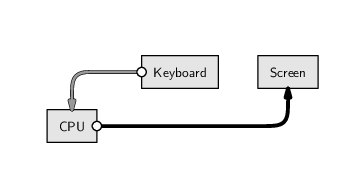
\includegraphics[width=0.5\linewidth]{img/script-commandline} \end{center}

\begin{center}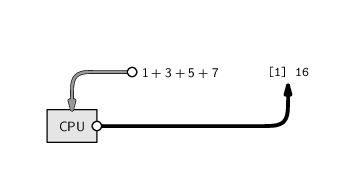
\includegraphics[width=0.5\linewidth]{img/script-commandlinedata} \end{center}

\begin{itemize}
\tightlist
\item
  Note que o resultado é apenas mostrado na tela, nada é salvo na
  memória (por enquanto).
\end{itemize}

\hypertarget{o-editor-de-scripts}{%
\subsection{O editor de scripts}\label{o-editor-de-scripts}}

\begin{itemize}
\tightlist
\item
  Para criar rotinas computacionais é necessário utilizar um editor
  de scripts.
\item
  Clique em \texttt{File\ \textgreater{}\ New\ file\ \textgreater{}\ R\ script}. Salve com a extensão
  \texttt{.R}.
\item
  Para enviar comandos diretamente para o console, selecione-os e
  aperte \texttt{Ctrl\ +\ \textless{}Enter\textgreater{}}.
\item
  Para adicionar comentários ao script, utiliza-se o símbolo
  \texttt{\#} antes do texto e/ou comandos. O que estiver depois do
  símbolo não será interpretado pelo R. Portanto:
\end{itemize}

\begin{Shaded}
\begin{Highlighting}[]
\DecValTok{2} \SpecialCharTok{+} \DecValTok{2}     \CommentTok{\# esta linha será executada}
\CommentTok{\# 2 + 2     esta linha não será executada}
\end{Highlighting}
\end{Shaded}

\hypertarget{operadores-aritmuxe9ticos}{%
\subsection{Operadores aritméticos}\label{operadores-aritmuxe9ticos}}

\begin{longtable}[]{@{}ll@{}}
\toprule()
Operador & Significado \\
\midrule()
\endhead
\texttt{+} & adição \\
\texttt{-} & subtração \\
\texttt{*} & multiplicação \\
\texttt{/} & divisão \\
\texttt{\^{}} ou \texttt{**} & potência \\
\texttt{sqrt()} & raíz quadrada \\
\texttt{exp()} & exponencial \\
\texttt{log()}; \texttt{log2()}; \texttt{log10()} & logaritmos \\
\texttt{factorial()} & fatorial \\
\bottomrule()
\end{longtable}

\hypertarget{ordens-de-execuuxe7uxe3o}{%
\subsection{Ordens de execução}\label{ordens-de-execuuxe7uxe3o}}

As operações são realizadas sempre seguindo as prioridades:

\begin{enumerate}
\def\labelenumi{\arabic{enumi}.}
\tightlist
\item
  De dentro para fora de parênteses \texttt{()}.
\item
  Potência e radiciação.
\item
  Multiplicação e divisão.
\item
  Adição e subtração.
\end{enumerate}

\begin{Shaded}
\begin{Highlighting}[]
\SpecialCharTok{\textgreater{}} \DecValTok{5} \SpecialCharTok{*} \DecValTok{2} \SpecialCharTok{{-}} \DecValTok{10} \SpecialCharTok{+} \DecValTok{7}
\NormalTok{[}\DecValTok{1}\NormalTok{] }\DecValTok{7}
\SpecialCharTok{\textgreater{}} \DecValTok{5} \SpecialCharTok{*} \DecValTok{2} \SpecialCharTok{{-}}\NormalTok{ (}\DecValTok{10} \SpecialCharTok{+} \DecValTok{7}\NormalTok{)}
\NormalTok{[}\DecValTok{1}\NormalTok{] }\SpecialCharTok{{-}}\DecValTok{7}
\SpecialCharTok{\textgreater{}} \DecValTok{5} \SpecialCharTok{*}\NormalTok{ (}\DecValTok{2} \SpecialCharTok{{-}} \DecValTok{10} \SpecialCharTok{+} \DecValTok{7}\NormalTok{)}
\NormalTok{[}\DecValTok{1}\NormalTok{] }\SpecialCharTok{{-}}\DecValTok{5}
\SpecialCharTok{\textgreater{}} \DecValTok{5} \SpecialCharTok{*}\NormalTok{ (}\DecValTok{2} \SpecialCharTok{{-}}\NormalTok{ (}\DecValTok{10} \SpecialCharTok{+} \DecValTok{7}\NormalTok{))}
\NormalTok{[}\DecValTok{1}\NormalTok{] }\SpecialCharTok{{-}}\DecValTok{75}
\SpecialCharTok{\textgreater{}} \DecValTok{2}\SpecialCharTok{*}\DecValTok{3}\SpecialCharTok{\^{}}\DecValTok{2}
\NormalTok{[}\DecValTok{1}\NormalTok{] }\DecValTok{18}
\SpecialCharTok{\textgreater{}} \DecValTok{2}\SpecialCharTok{*}\DecValTok{3}\SpecialCharTok{**}\DecValTok{2}
\NormalTok{[}\DecValTok{1}\NormalTok{] }\DecValTok{18}
\SpecialCharTok{\textgreater{}} \DecValTok{3}\SpecialCharTok{*}\FunctionTok{sqrt}\NormalTok{(}\DecValTok{9}\SpecialCharTok{**}\DecValTok{2}\NormalTok{)}
\NormalTok{[}\DecValTok{1}\NormalTok{] }\DecValTok{27}
\SpecialCharTok{\textgreater{}} \FunctionTok{exp}\NormalTok{(}\DecValTok{1}\NormalTok{)}
\NormalTok{[}\DecValTok{1}\NormalTok{] }\FloatTok{2.718282}
\SpecialCharTok{\textgreater{}} \FunctionTok{log2}\NormalTok{(}\DecValTok{16}\NormalTok{)}
\NormalTok{[}\DecValTok{1}\NormalTok{] }\DecValTok{4}
\end{Highlighting}
\end{Shaded}

\hypertarget{exercuxedcios}{%
\subsection*{Exercícios}\label{exercuxedcios}}


\begin{enumerate}
\def\labelenumi{\arabic{enumi}.}
\tightlist
\item
  Calcule a seguinte equação: \(32 + 16^2 - 25^3\)
\item
  Divida o resultado por \(345\)
\item
  Qual o resultado da expressão \(\frac{e^{-2} 2^{4} - 1}{4!}\)?
\item
  E do logaritmo desta expressão?
\end{enumerate}

\hypertarget{salvando-resultados}{%
\subsection{``Salvando'' resultados}\label{salvando-resultados}}

Do exercício anterior

\begin{Shaded}
\begin{Highlighting}[]
\SpecialCharTok{\textgreater{}}\NormalTok{ x }\OtherTok{\textless{}{-}} \DecValTok{32} \SpecialCharTok{+} \DecValTok{16}\SpecialCharTok{\^{}}\DecValTok{2} \SpecialCharTok{{-}} \DecValTok{25}\SpecialCharTok{\^{}}\DecValTok{3}
\SpecialCharTok{\textgreater{}}\NormalTok{ x}
\NormalTok{[}\DecValTok{1}\NormalTok{] }\SpecialCharTok{{-}}\DecValTok{15337}
\SpecialCharTok{\textgreater{}}\NormalTok{ x}\SpecialCharTok{/}\DecValTok{345}
\NormalTok{[}\DecValTok{1}\NormalTok{] }\SpecialCharTok{{-}}\FloatTok{44.45507}
\SpecialCharTok{\textgreater{}}\NormalTok{ (y }\OtherTok{\textless{}{-}}\NormalTok{ (}\FunctionTok{exp}\NormalTok{(}\SpecialCharTok{{-}}\DecValTok{2}\NormalTok{) }\SpecialCharTok{*} \DecValTok{2}\SpecialCharTok{\^{}}\DecValTok{4} \SpecialCharTok{{-}} \DecValTok{1}\NormalTok{)}\SpecialCharTok{/}\FunctionTok{factorial}\NormalTok{(}\DecValTok{4}\NormalTok{))}
\NormalTok{[}\DecValTok{1}\NormalTok{] }\FloatTok{0.04855686}
\SpecialCharTok{\textgreater{}} \FunctionTok{log}\NormalTok{(y)}
\NormalTok{[}\DecValTok{1}\NormalTok{] }\SpecialCharTok{{-}}\FloatTok{3.02502}
\end{Highlighting}
\end{Shaded}

Quando criamos uma variável (\texttt{x}, \texttt{y}), ela fica armazenada
\textbf{temporariamente} na memória RAM.

\begin{center}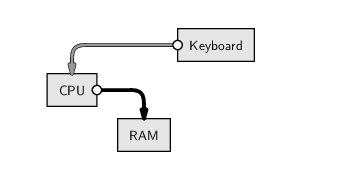
\includegraphics[width=0.5\linewidth]{img/script-assign} \end{center}

Para saber quais objetos foram criados, usamos a \textbf{função} \texttt{ls()}

\begin{Shaded}
\begin{Highlighting}[]
\SpecialCharTok{\textgreater{}} \FunctionTok{ls}\NormalTok{()}
\NormalTok{[}\DecValTok{1}\NormalTok{] }\StringTok{"x"} \StringTok{"y"}
\end{Highlighting}
\end{Shaded}

Estas variáveis ficam armazenadas no chamado \emph{workspace} do R.

\begin{itemize}
\tightlist
\item
  O \emph{workspace} consiste de tudo que foi criado durante uma sessão do R,
  e fica armazenado na memória RAM.
\end{itemize}

Para efetivamente salvar essas variáveis, podemos armazenar esse \emph{workspace}
do R em disco, em um arquivo chamado \texttt{.Rdata}

\begin{center}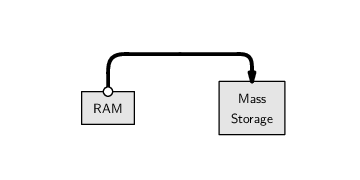
\includegraphics[width=0.5\linewidth]{img/script-workspace} \end{center}

\begin{center}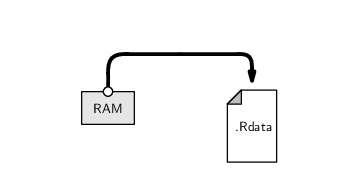
\includegraphics[width=0.5\linewidth]{img/script-workspacedata} \end{center}

\begin{itemize}
\tightlist
\item
  Quando o R é iniciado em um diretório com um arquivo \texttt{.Rdata}, as
  variáveis salvas são automaticamente carregadas.
\item
  No entanto, é sempre melhor salvar os dados e o \textbf{script}, assim é
  possível gerar os resultados novamente, sem salvar nada sem
  necessidade.
\item
  Veremos mais pra frente como salvar variáveis específicas, por
  exemplo, resultados de uma análise que leva muito tempo para ser
  executada.
\item
  O mais importante é salvar o \textbf{código}, assim sabemos \textbf{como}
  chegamos a determinado resultado, e podemos recriá-lo.
\end{itemize}

\hypertarget{finalizando-o-programa}{%
\subsection{Finalizando o programa}\label{finalizando-o-programa}}

A qualquer momento durante uma sessão você pode usar o comando

\begin{Shaded}
\begin{Highlighting}[]
\SpecialCharTok{\textgreater{}} \FunctionTok{save.image}\NormalTok{()}
\end{Highlighting}
\end{Shaded}

No RStudio:

\begin{itemize}
\tightlist
\item
  \texttt{File\ \textgreater{}\ Save\ As...}
\item
  Na janela que abrir, digite o nome do arquivo (por exemplo
  \texttt{script\_aula1}) e salve.
\item
  Automaticamente o script será salvo com a extensão \texttt{.R}
  (nesse caso \texttt{script\_aula1.R}) no diretório de trabalho que você
  configurou no início.
\end{itemize}

Alternativamente, você pode também salvar toda sua área de trabalho,
clicando em \texttt{Workspace\ \textgreater{}\ Save\ As\ Default\ Workspace}. Este
processo irá gerar dois arquivos:

\begin{itemize}
\tightlist
\item
  \texttt{.Rdata}: contém todos os objetos criados durante uma
  sessão. Não é necessário (e nem recomendado) dar um nome antes do
  ponto. Dessa forma, a próxima vez que o programa for iniciado neste
  diretório, a área de trabalho será carregada automaticamente.
\item
  \texttt{.Rhistory}: um arquivo texto que contém todos os comandos
  que foram digitados no console.
\end{itemize}

\hypertarget{encoding}{%
\subsection{Encoding}\label{encoding}}

Caracteres especiais (cedilha, acentos, dentre outros) podem gerar problemas de visualização
entre diferentes sistemas operacionais que utilizam diferentes codificações (\emph{encodings}).
Não iremos tratar disto neste momento, mas se voce visualizar estes caracteres de maneira ``estranha'' é porque
irá precisar conciliar os ``encodings''.

\hypertarget{referuxeancias}{%
\section*{Referências}\label{referuxeancias}}


\begin{itemize}
\tightlist
\item
  Leek, J. \href{https://leanpub.com/datastyle}{The Elements of Data Analytic Style}. Leanpub, 2015.
\item
  Murrell,
  P. \href{https://www.stat.auckland.ac.nz/~paul/ItDT/HTML}{Introduction to data technologies}. Boca
  Raton: Chapman \& Hall/CRC, 2009.
\item
  Peng,
  RD. \href{https://leanpub.com/rprogramming}{R programming for data science}. Leanpub, 2015.
\end{itemize}

\hypertarget{objetos-e-classes}{%
\chapter{Objetos e classes}\label{objetos-e-classes}}

\hypertarget{funuxe7uxf5es-e-argumentos}{%
\section{Funções e argumentos}\label{funuxe7uxf5es-e-argumentos}}

As funções no R são definidas como:

\begin{Shaded}
\begin{Highlighting}[]
\FunctionTok{nome}\NormalTok{(argumento1, argumento2, ...)}
\end{Highlighting}
\end{Shaded}

Exemplo: função \texttt{runif()} (para gerar valores aleatórios de uma
distribuição uniforme):

\begin{Shaded}
\begin{Highlighting}[]
\FunctionTok{runif}\NormalTok{(n, }\AttributeTok{min =} \DecValTok{0}\NormalTok{, }\AttributeTok{max =} \DecValTok{1}\NormalTok{)}
\end{Highlighting}
\end{Shaded}

\begin{Shaded}
\begin{Highlighting}[]
\FunctionTok{runif}\NormalTok{(}\DecValTok{10}\NormalTok{, }\DecValTok{1}\NormalTok{, }\DecValTok{100}\NormalTok{)}
\NormalTok{ [}\DecValTok{1}\NormalTok{] }\FloatTok{31.468845} \FloatTok{26.509578} \FloatTok{55.679921}  \FloatTok{6.581932} \FloatTok{47.386379} \FloatTok{48.893303} \FloatTok{81.427859}
\NormalTok{ [}\DecValTok{8}\NormalTok{] }\FloatTok{37.661733} \FloatTok{55.109301} \FloatTok{17.855943}
\end{Highlighting}
\end{Shaded}

Argumentos que já possuem um valor especificado (como \texttt{max} e \texttt{min})
podem ser omitidos:

\begin{Shaded}
\begin{Highlighting}[]
\FunctionTok{runif}\NormalTok{(}\DecValTok{10}\NormalTok{)}
\end{Highlighting}
\end{Shaded}

Se os argumentos forem nomeados, a ordem deles dentro da função não tem
mais importância:

\begin{Shaded}
\begin{Highlighting}[]
\FunctionTok{runif}\NormalTok{(}\AttributeTok{min =} \DecValTok{1}\NormalTok{, }\AttributeTok{max =} \DecValTok{100}\NormalTok{, }\AttributeTok{n =} \DecValTok{10}\NormalTok{)}
\end{Highlighting}
\end{Shaded}

Argumentos nomeados e não nomeados podem ser utilizados, desde que os
não nomeados estejam na posição correta:

\begin{Shaded}
\begin{Highlighting}[]
\FunctionTok{runif}\NormalTok{(}\DecValTok{10}\NormalTok{, }\AttributeTok{max =} \DecValTok{100}\NormalTok{, }\AttributeTok{min =} \DecValTok{1}\NormalTok{)}
\end{Highlighting}
\end{Shaded}

\hypertarget{outros-tipos-de-argumentos}{%
\subsection{Outros tipos de argumentos}\label{outros-tipos-de-argumentos}}

Exemplo: função \texttt{sample()}:

\begin{Shaded}
\begin{Highlighting}[]
\FunctionTok{sample}\NormalTok{(x, size, }\AttributeTok{replace =} \ConstantTok{FALSE}\NormalTok{, }\AttributeTok{prob =} \ConstantTok{NULL}\NormalTok{)}
\end{Highlighting}
\end{Shaded}

\begin{itemize}
\tightlist
\item
  \texttt{x} e \texttt{size} devem ser obrigatoriamente especificados.
\item
  \texttt{replace} é lógico: \texttt{TRUE} (\texttt{T}) ou \texttt{FALSE} (\texttt{F}).
\item
  \texttt{prob} é um argumento vazio ou ausente (``opcional'').
\end{itemize}

Exemplo: função \texttt{plot()}:

\begin{Shaded}
\begin{Highlighting}[]
\FunctionTok{plot}\NormalTok{(x, y, ...)}
\end{Highlighting}
\end{Shaded}

\begin{itemize}
\tightlist
\item
  ``\texttt{...}'' permite especificar argumentos de outras funções (por exemplo
  \texttt{par()}).
\end{itemize}

Para ver todos os argumentos disponíveis de uma função, podemos usar a
função \texttt{args()}.

\begin{Shaded}
\begin{Highlighting}[]
\FunctionTok{args}\NormalTok{(sample)}
\ControlFlowTok{function}\NormalTok{ (x, size, }\AttributeTok{replace =} \ConstantTok{FALSE}\NormalTok{, }\AttributeTok{prob =} \ConstantTok{NULL}\NormalTok{) }
\ConstantTok{NULL}
\end{Highlighting}
\end{Shaded}

\hypertarget{mecanismos-de-ajuda}{%
\section{Mecanismos de ajuda}\label{mecanismos-de-ajuda}}

Argumentos e detalhes do funcionamento das funções:

\begin{Shaded}
\begin{Highlighting}[]
\NormalTok{?runif}
\end{Highlighting}
\end{Shaded}

ou

\begin{Shaded}
\begin{Highlighting}[]
\FunctionTok{help}\NormalTok{(runif)}
\end{Highlighting}
\end{Shaded}

A documentação contém os campos:

\begin{itemize}
\tightlist
\item
  \textbf{Description:} breve descrição.
\item
  \textbf{Usage:} função e todos seus argumentos.
\item
  \textbf{Arguments:} lista descrevendo cada argumento.
\item
  \textbf{Details:} descrição detalhada.
\item
  \textbf{Value:} o que a função retorna.
\item
  \textbf{References:} bibliografia relacionada.
\item
  \textbf{See Also:} funções relacionadas.
\item
  \textbf{Examples:} exemplos práticos.
\end{itemize}

Procura por nomes de funções que contenham algum termo:

\begin{Shaded}
\begin{Highlighting}[]
\FunctionTok{apropos}\NormalTok{(}\StringTok{"mod"}\NormalTok{)}
\FunctionTok{apropos}\NormalTok{(}\StringTok{"model"}\NormalTok{)}
\end{Highlighting}
\end{Shaded}

Procura por funções que contenham \texttt{palavra} em qualquer parte de sua
documentação:

\begin{Shaded}
\begin{Highlighting}[]
\FunctionTok{help.search}\NormalTok{(}\StringTok{"palavra"}\NormalTok{)}
\end{Highlighting}
\end{Shaded}

Ajuda através do navegador (também contém manuais, \ldots):

\begin{Shaded}
\begin{Highlighting}[]
\FunctionTok{help.start}\NormalTok{()}
\end{Highlighting}
\end{Shaded}

Sites para busca na documentação dos diversos pacotes:

\begin{itemize}
\tightlist
\item
  RDocumentation \url{https://www.rdocumentation.org/}.
\item
  R Package Documentation \url{https://rdrr.io/}.
\item
  R Contributed Documentation (várias línguas).
  \url{https://cran.r-project.org/other-docs.html}.
\end{itemize}

Os pacotes do R contêm funções específicas para determinadas tarefas, e
estendem a instalação básica do R. Atualmente existem mais de 10000
pacotes disponíveis no
\href{http://cran-r.c3sl.ufpr.br/web/packages/index.html}{CRAN}, além de
diversos outros hospedados em sites como \href{https://github.com}{Github},
por exemplo.

Ao instalar o R, os seguintes pacotes já vêm instalados (fazem parte do
chamado ``R core''):

\begin{verbatim}
 [1] "base"       "boot"       "class"      "cluster"    "codetools" 
 [6] "compiler"   "datasets"   "foreign"    "graphics"   "grDevices" 
[11] "grid"       "KernSmooth" "lattice"    "MASS"       "Matrix"    
[16] "methods"    "mgcv"       "nlme"       "nnet"       "parallel"  
[21] "rpart"      "spatial"    "splines"    "stats"      "stats4"    
[26] "survival"   "tcltk"      "tools"      "utils"     
\end{verbatim}

No entanto, nem todos são carregados na inicialização do R. Por padrão,
apenas os seguintes pacotes são carregados automaticamente:

\begin{verbatim}
[1] "graphics"  "grDevices" "datasets"  "utils"     "methods"   "base"     
\end{verbatim}

Para listar os pacotes carregados, use a função

\begin{Shaded}
\begin{Highlighting}[]
\FunctionTok{search}\NormalTok{()}
\end{Highlighting}
\end{Shaded}

Note que o primeiro elemento, \texttt{.GlobalEnv}, será sempre carregado pois
ele é o \emph{ambiente} que irá armazenar (e deixar disponível) os objetos
criados pelo usuário. Para carregar um pacote instalado, usamos a função
\texttt{library()}, por exemplo

\begin{Shaded}
\begin{Highlighting}[]
\FunctionTok{library}\NormalTok{(lattice)}
\FunctionTok{search}\NormalTok{()}
\end{Highlighting}
\end{Shaded}

Isso tornará todas as funções do pacote \texttt{lattice} disponíveis para uso.

Para instalar um pacote usamos a função \texttt{install.packages()}. Sabendo o
nome do pacote, por exemplo, \texttt{mvtnorm}, fazemos

\begin{Shaded}
\begin{Highlighting}[]
\FunctionTok{install.packages}\NormalTok{(}\StringTok{"mvtnorm"}\NormalTok{)}
\end{Highlighting}
\end{Shaded}

Se o diretório padrão de instalação de um pacote for de acesso restrito
(root por exemplo), o R irá perguntar se você gostaria de instalar o
pacote em uma biblioteca pessoal, e sugerirá um diretório que possui as
permissões necessárias. Você pode se antecipar e já definir e criar um
diretório na sua pasta pessoal, e instalar os pacotes sempre nesse
local. Por exemplo, defina \texttt{\textasciitilde{}/R/library} como sua biblioteca pessoal.
Para instalar os pacotes sempre nesse diretório faça:

\begin{Shaded}
\begin{Highlighting}[]
\FunctionTok{install.packages}\NormalTok{(}\StringTok{"mvtnorm"}\NormalTok{, }\AttributeTok{lib =} \StringTok{"\textasciitilde{}/R/library"}\NormalTok{)}
\end{Highlighting}
\end{Shaded}

Para verificar as bibliotecas disponíveis e se existem pacotes para serem
atualizados, use

\begin{Shaded}
\begin{Highlighting}[]
\FunctionTok{packageStatus}\NormalTok{()}
\end{Highlighting}
\end{Shaded}

Para atualizar automaticamente todos os pacotes faça

\begin{Shaded}
\begin{Highlighting}[]
\FunctionTok{update.packages}\NormalTok{(}\AttributeTok{ask =} \ConstantTok{FALSE}\NormalTok{)}
\end{Highlighting}
\end{Shaded}

\hypertarget{criando-uma-funuxe7uxe3o}{%
\section{Criando uma função}\label{criando-uma-funuxe7uxe3o}}

A ideia original do R é transformar usuários em programadores

\begin{quote}
\emph{``\ldots{} to turn ideas into software, quickly and faithfully.''}

-- John M. Chambers.
\end{quote}

Criar funções para realizar trabalhos específicos é um dos grandes
poderes do R.

Por exemplo, podemos criar a famosa função

\begin{Shaded}
\begin{Highlighting}[]
\NormalTok{ola.mundo }\OtherTok{\textless{}{-}} \ControlFlowTok{function}\NormalTok{()\{}
    \FunctionTok{writeLines}\NormalTok{(}\StringTok{"Olá mundo"}\NormalTok{)}
\NormalTok{\}}
\end{Highlighting}
\end{Shaded}

E chama-la através de

\begin{Shaded}
\begin{Highlighting}[]
\FunctionTok{ola.mundo}\NormalTok{()}
\NormalTok{Olá mundo}
\end{Highlighting}
\end{Shaded}

A função acima não permite alterar o resultado da saída. Podemos fazer
isso incluindo um \textbf{argumento}

\begin{Shaded}
\begin{Highlighting}[]
\NormalTok{ola.mundo }\OtherTok{\textless{}{-}} \ControlFlowTok{function}\NormalTok{(texto)\{}
    \FunctionTok{writeLines}\NormalTok{(texto)}
\NormalTok{\}}
\end{Highlighting}
\end{Shaded}

E fazer por exemplo

\begin{Shaded}
\begin{Highlighting}[]
\FunctionTok{ola.mundo}\NormalTok{(}\StringTok{"Funções são legais"}\NormalTok{)}
\NormalTok{Funções são legais}
\end{Highlighting}
\end{Shaded}

(Veremos detalhes de funções mais adiante)

\hypertarget{exercuxedcios-1}{%
\section*{Exercícios}\label{exercuxedcios-1}}


\begin{enumerate}
\def\labelenumi{\arabic{enumi}.}
\tightlist
\item
  Usando a função \texttt{runif()} gere \(30\) números aleatórios entre:

  \begin{itemize}
  \tightlist
  \item
    0 e 1
  \item
    -5 e 5
  \item
    10 e 500
  \end{itemize}
\end{enumerate}

alternando a posição dos argumentos da função.

\begin{enumerate}
\def\labelenumi{\arabic{enumi}.}
\setcounter{enumi}{1}
\tightlist
\item
  Veja o help da função (?) \texttt{"+"}
\item
  Crie uma função para fazer a soma de dois números: \texttt{x} e \texttt{y}
\item
  Crie uma função para simular a jogada de um dado.
\item
  Crie uma função para simular a jogada de dois dados.
\end{enumerate}

\hypertarget{objetos}{%
\section{Objetos}\label{objetos}}

O que é um objeto?

\begin{itemize}
\tightlist
\item
  Um \textbf{símbolo} ou uma \textbf{variável} capaz de armazenar qualquer valor
  ou estrutura de dados.
\end{itemize}

Por quê objetos?

\begin{itemize}
\tightlist
\item
  Uma maneira simples de acessar os dados armazenados na memória (o R
  não permite acesso direto à memória).
\end{itemize}

Programação:

\begin{itemize}
\tightlist
\item
  Objetos \(\Rightarrow\) Classes \(\Rightarrow\) Métodos.
\end{itemize}

\begin{quote}
\emph{``Tudo no R é um objeto.''}
\end{quote}

\begin{quote}
\emph{``Todo objeto no R tem uma classe.''}
\end{quote}

\begin{itemize}
\tightlist
\item
  \textbf{Classe:} é a definição de um objeto. Descreve a forma do objeto e
  como ele será manipulado pelas diferentes funções.
\item
  \textbf{Método:} são \textbf{funções genéricas} que executam suas tarefas de
  acordo com cada classe. Duas das funções genéricas mais importantes
  são:

  \begin{itemize}
  \tightlist
  \item
    \texttt{summary().}
  \item
    \texttt{plot().}
  \end{itemize}
\end{itemize}

Veja o resultado de

\begin{Shaded}
\begin{Highlighting}[]
\FunctionTok{methods}\NormalTok{(summary)}
\FunctionTok{methods}\NormalTok{(plot)}
\end{Highlighting}
\end{Shaded}

(Veremos mais detalhes adiante).

A variável \texttt{x} recebe o valor \(2\) (tornando-se um objeto dentro do R):

\begin{Shaded}
\begin{Highlighting}[]
\NormalTok{x }\OtherTok{\textless{}{-}} \DecValTok{2}
\end{Highlighting}
\end{Shaded}

O símbolo \texttt{\textless{}-} é chamado de \textbf{operador de atribuição}. Ele serve para
atribuir valores a objetos, e é formado pelos símbolos \texttt{\textless{}} e \texttt{-},
obrigatoriamente \textbf{sem espaços}.

Para ver o conteúdo do objeto:

\begin{Shaded}
\begin{Highlighting}[]
\NormalTok{x}
\NormalTok{[}\DecValTok{1}\NormalTok{] }\DecValTok{2}
\end{Highlighting}
\end{Shaded}

\textbf{Observação}: O símbolo \texttt{=} pode ser usado no lugar de \texttt{\textless{}-} mas não
é recomendado.

Quando você faz

\begin{Shaded}
\begin{Highlighting}[]
\NormalTok{x }\OtherTok{\textless{}{-}} \DecValTok{2}
\end{Highlighting}
\end{Shaded}

está fazendo uma \textbf{declaração}, ou seja, declarando que a variável \texttt{x}
irá agora se tornar um objeto que armazena o número \texttt{2}. As declarações
podem ser feitas uma em cada linha

\begin{Shaded}
\begin{Highlighting}[]
\NormalTok{x }\OtherTok{\textless{}{-}} \DecValTok{2}
\NormalTok{y }\OtherTok{\textless{}{-}} \DecValTok{4}
\end{Highlighting}
\end{Shaded}

ou separadas por \texttt{;}

\begin{Shaded}
\begin{Highlighting}[]
\NormalTok{x }\OtherTok{\textless{}{-}} \DecValTok{2}\NormalTok{; y }\OtherTok{\textless{}{-}} \DecValTok{4}
\end{Highlighting}
\end{Shaded}

Operações matemáticas em objetos:

\begin{Shaded}
\begin{Highlighting}[]
\NormalTok{x }\SpecialCharTok{+}\NormalTok{ x}
\NormalTok{[}\DecValTok{1}\NormalTok{] }\DecValTok{4}
\end{Highlighting}
\end{Shaded}

Objetos podem armazenar diferentes estruturas de dados:

\begin{Shaded}
\begin{Highlighting}[]
\NormalTok{y }\OtherTok{\textless{}{-}} \FunctionTok{runif}\NormalTok{(}\DecValTok{10}\NormalTok{)}
\NormalTok{y}
\NormalTok{ [}\DecValTok{1}\NormalTok{] }\FloatTok{0.6249965} \FloatTok{0.8821655} \FloatTok{0.2803538} \FloatTok{0.3984879} \FloatTok{0.7625511} \FloatTok{0.6690217} \FloatTok{0.2046122}
\NormalTok{ [}\DecValTok{8}\NormalTok{] }\FloatTok{0.3575249} \FloatTok{0.3594751} \FloatTok{0.6902905}
\end{Highlighting}
\end{Shaded}

Note que cada objeto só pode armazenar uma estrutura (um número ou uma
sequência de valores) de cada vez! (Aqui, o valor \(4\) que estava
armazenado em \texttt{y} foi sobrescrito pelos valores acima).

\hypertarget{nomes-de-objetos}{%
\subsection{Nomes de objetos}\label{nomes-de-objetos}}

\begin{itemize}
\tightlist
\item
  Podem ser formados por letras, números, ``\texttt{\_}'', e ``\texttt{.}''.
\item
  Não podem começar com número e/ou ponto.
\item
  Não podem conter espaços.
\item
  Evite usar acentos.
\item
  Evite usar nomes de funções como:
\end{itemize}

\texttt{c\ q\ t\ C\ D\ F\ I\ T\ diff\ df\ data\ var\ pt}

\begin{itemize}
\tightlist
\item
  O R é \emph{case-sensitive}, portanto:
\end{itemize}

\texttt{dados} \(\neq\) \texttt{Dados} \(\neq\) \texttt{DADOS}.

\hypertarget{gerenciando-a-uxe1rea-de-trabalho}{%
\subsection{Gerenciando a área de trabalho}\label{gerenciando-a-uxe1rea-de-trabalho}}

Liste os objetos criados com a função \texttt{ls()}:

\begin{Shaded}
\begin{Highlighting}[]
\FunctionTok{ls}\NormalTok{()}
\end{Highlighting}
\end{Shaded}

Para remover apenas um objeto:

\begin{Shaded}
\begin{Highlighting}[]
\FunctionTok{rm}\NormalTok{(x)}
\end{Highlighting}
\end{Shaded}

Para remover outros objetos:

\begin{Shaded}
\begin{Highlighting}[]
\FunctionTok{rm}\NormalTok{(x, y)}
\end{Highlighting}
\end{Shaded}

Para remover todos os objetos:

\begin{Shaded}
\begin{Highlighting}[]
\FunctionTok{rm}\NormalTok{(}\AttributeTok{list =} \FunctionTok{ls}\NormalTok{())}
\end{Highlighting}
\end{Shaded}

\textbf{Cuidado!} O comando acima apaga todos os objetos na sua área de
trabalho sem perguntar. Depois só é possível recuperar os objetos ao
rodar o script novamente.

\hypertarget{exercuxedcios-2}{%
\section*{Exercícios}\label{exercuxedcios-2}}


\begin{enumerate}
\def\labelenumi{\arabic{enumi}.}
\tightlist
\item
  Armazene o resultado da equação \(32 + 16^2 - 25^3\) no objeto \texttt{x}.
\item
  Divida \texttt{x} por \(345\) e armazene em \texttt{y}.
\item
  Crie um objeto (com o nome que você quiser) para armazenar \(30\)
  valores aleatórios de uma distribuição uniforme entre \(10\) e \(50\).
\item
  Remova o objeto \texttt{y}.
\item
  Remova os demais objetos de uma única vez.
\item
  Procure a função utilizada para gerar numeros aleatórios de uma
  distribuição de Poisson, e gere \(100\) valores para a VA \(X \sim \text{Poisson}(5)\).
\end{enumerate}

\hypertarget{tipos-e-classes-de-objetos}{%
\section{Tipos e classes de objetos}\label{tipos-e-classes-de-objetos}}

Para saber como trabalhar com dados no R, é fundamental entender as
possíveis estruturas (ou tipos) de dados possíveis. O formato mais
básico de dados são os vetores, e a partir deles, outras estruturas mais
complexas podem ser construídas. O R possui dois tipos básicos de
vetores:

\begin{itemize}
\item
  \textbf{Vetores atômicos}: existem seis tipos básicos:

  \begin{itemize}
  \tightlist
  \item
    \texttt{double}.
  \item
    \texttt{integer}.
  \item
    \texttt{character}.
  \item
    \texttt{logical}.
  \item
    \texttt{complex}.
  \item
    \texttt{raw}.
  \end{itemize}

  Os tipos \texttt{integer} e \texttt{double} são chamados conjuntamente de \texttt{numeric}.
\item
  \textbf{Listas}: também chamadas de \emph{vetores recursivos} pois listas podem
  conter outras listas.
\end{itemize}

A principal diferença entre vetores atômicos e listas é que o primeiro é
\textbf{homogêneo} (cada vetor só pode conter um tipo), enquanto que o
segundo pode ser \textbf{heterogêneo} (cada vetor pode conter mais de um
tipo).

Um vetor atômico só pode conter elementos de um mesmo tipo.

Um vetor, como o próprio nome diz, é uma estrutura unidimensional, mas
na maioria das vezes iremos trabalhar com estruturas de dados
bidimensionais (linhas e colunas). Portanto diferentes estruturas (com
diferentes dimensões) podem ser criadas a partir dos vetores atômicos.
Quando isso acontece, temos o que é chamado de \textbf{classe} de um objeto.
Embora os vetores atômicos só possuam seis tipos básicos, existe um
número muito grande de classes, e novas são inventadas todos os dias. E
mesmo que um objeto seja de qualquer classe, ele sempre será de um dos
seis tipos básicos (ou uma lista).

Para verificar o tipo de um objeto, usamos a função \texttt{typeof()}, enquanto
que a classe é verificada com a função \texttt{class()}. Vejamos alguns
exemplos:

\begin{Shaded}
\begin{Highlighting}[]
\DocumentationTok{\#\# double}
\NormalTok{x }\OtherTok{\textless{}{-}} \FunctionTok{c}\NormalTok{(}\DecValTok{2}\NormalTok{, }\DecValTok{4}\NormalTok{, }\DecValTok{6}\NormalTok{)}
\FunctionTok{typeof}\NormalTok{(x)}
\NormalTok{[}\DecValTok{1}\NormalTok{] }\StringTok{"double"}
\FunctionTok{class}\NormalTok{(x)}
\NormalTok{[}\DecValTok{1}\NormalTok{] }\StringTok{"numeric"}
\DocumentationTok{\#\# integer}
\NormalTok{x }\OtherTok{\textless{}{-}} \FunctionTok{c}\NormalTok{(2L, 4L, 6L)}
\FunctionTok{typeof}\NormalTok{(x)}
\NormalTok{[}\DecValTok{1}\NormalTok{] }\StringTok{"integer"}
\FunctionTok{class}\NormalTok{(x)}
\NormalTok{[}\DecValTok{1}\NormalTok{] }\StringTok{"integer"}
\DocumentationTok{\#\# character}
\NormalTok{x }\OtherTok{\textless{}{-}} \FunctionTok{c}\NormalTok{(}\StringTok{"a"}\NormalTok{, }\StringTok{"b"}\NormalTok{, }\StringTok{"c"}\NormalTok{)}
\FunctionTok{typeof}\NormalTok{(x)}
\NormalTok{[}\DecValTok{1}\NormalTok{] }\StringTok{"character"}
\FunctionTok{class}\NormalTok{(x)}
\NormalTok{[}\DecValTok{1}\NormalTok{] }\StringTok{"character"}
\DocumentationTok{\#\# logical}
\NormalTok{x }\OtherTok{\textless{}{-}} \FunctionTok{c}\NormalTok{(}\ConstantTok{TRUE}\NormalTok{, }\ConstantTok{FALSE}\NormalTok{, }\ConstantTok{TRUE}\NormalTok{)}
\FunctionTok{typeof}\NormalTok{(x)}
\NormalTok{[}\DecValTok{1}\NormalTok{] }\StringTok{"logical"}
\FunctionTok{class}\NormalTok{(x)}
\NormalTok{[}\DecValTok{1}\NormalTok{] }\StringTok{"logical"}
\DocumentationTok{\#\# complex}
\NormalTok{x }\OtherTok{\textless{}{-}} \FunctionTok{c}\NormalTok{(}\DecValTok{2} \SpecialCharTok{+}\NormalTok{ 1i, }\DecValTok{4} \SpecialCharTok{+}\NormalTok{ 1i, }\DecValTok{6} \SpecialCharTok{+}\NormalTok{ 1i)}
\FunctionTok{typeof}\NormalTok{(x)}
\NormalTok{[}\DecValTok{1}\NormalTok{] }\StringTok{"complex"}
\FunctionTok{class}\NormalTok{(x)}
\NormalTok{[}\DecValTok{1}\NormalTok{] }\StringTok{"complex"}
\DocumentationTok{\#\# raw}
\NormalTok{x }\OtherTok{\textless{}{-}} \FunctionTok{raw}\NormalTok{(}\DecValTok{3}\NormalTok{)}
\FunctionTok{typeof}\NormalTok{(x)}
\NormalTok{[}\DecValTok{1}\NormalTok{] }\StringTok{"raw"}
\FunctionTok{class}\NormalTok{(x)}
\NormalTok{[}\DecValTok{1}\NormalTok{] }\StringTok{"raw"}
\end{Highlighting}
\end{Shaded}

\hypertarget{vetores-numuxe9ricos}{%
\subsection{Vetores numéricos}\label{vetores-numuxe9ricos}}

Características:

\begin{itemize}
\tightlist
\item
  Coleção ordenada de valores.
\item
  Estrutura unidimensional.
\end{itemize}

Usando a função \texttt{c()} para criar vetores:

\begin{Shaded}
\begin{Highlighting}[]
\NormalTok{num }\OtherTok{\textless{}{-}} \FunctionTok{c}\NormalTok{(}\DecValTok{10}\NormalTok{, }\DecValTok{5}\NormalTok{, }\DecValTok{2}\NormalTok{, }\DecValTok{4}\NormalTok{, }\DecValTok{8}\NormalTok{, }\DecValTok{9}\NormalTok{)}
\NormalTok{num}
\NormalTok{[}\DecValTok{1}\NormalTok{] }\DecValTok{10}  \DecValTok{5}  \DecValTok{2}  \DecValTok{4}  \DecValTok{8}  \DecValTok{9}
\FunctionTok{typeof}\NormalTok{(num)}
\NormalTok{[}\DecValTok{1}\NormalTok{] }\StringTok{"double"}
\FunctionTok{class}\NormalTok{(num)}
\NormalTok{[}\DecValTok{1}\NormalTok{] }\StringTok{"numeric"}
\end{Highlighting}
\end{Shaded}

Por que \texttt{numeric} e não \texttt{integer}?

\begin{Shaded}
\begin{Highlighting}[]
\NormalTok{x }\OtherTok{\textless{}{-}} \FunctionTok{c}\NormalTok{(10L, 5L, 2L, 4L, 8L, 9L)}
\NormalTok{x}
\NormalTok{[}\DecValTok{1}\NormalTok{] }\DecValTok{10}  \DecValTok{5}  \DecValTok{2}  \DecValTok{4}  \DecValTok{8}  \DecValTok{9}
\FunctionTok{typeof}\NormalTok{(x)}
\NormalTok{[}\DecValTok{1}\NormalTok{] }\StringTok{"integer"}
\FunctionTok{class}\NormalTok{(x)}
\NormalTok{[}\DecValTok{1}\NormalTok{] }\StringTok{"integer"}
\end{Highlighting}
\end{Shaded}

Para forçar a representação de um número para inteiro é necessário usar
o sufixo \texttt{L}.

Note que a diferença entre \texttt{numeric} e \texttt{integer} também possui impacto
computacional, pois o armazenamento de números inteiros ocupa menos
espaço na memória. Dessa forma, esperamos que o vetor \texttt{x} acima ocupe
menos espaço na memória do que o vetor \texttt{num}, embora sejam aparentemente
idênticos. Veja:

\begin{Shaded}
\begin{Highlighting}[]
\FunctionTok{object.size}\NormalTok{(num)}
\DecValTok{96}\NormalTok{ bytes}
\FunctionTok{object.size}\NormalTok{(x)}
\DecValTok{80}\NormalTok{ bytes}
\end{Highlighting}
\end{Shaded}

A diferença pode parecer pequena, mas pode ter um grande impacto
computacional quando os vetores são formados por milhares ou milhões de
números.

\hypertarget{representauxe7uxe3o-numuxe9rica-dentro-do-r}{%
\subsubsection{Representação numérica dentro do R}\label{representauxe7uxe3o-numuxe9rica-dentro-do-r}}

Os números que aparecem na tela do console do R são apenas
representações simplificadas do número real armazenado na memória.
Por exemplo,

\begin{Shaded}
\begin{Highlighting}[]
\NormalTok{x }\OtherTok{\textless{}{-}} \FunctionTok{runif}\NormalTok{(}\DecValTok{10}\NormalTok{)}
\NormalTok{x}
\NormalTok{ [}\DecValTok{1}\NormalTok{] }\FloatTok{0.2875775} \FloatTok{0.7883051} \FloatTok{0.4089769} \FloatTok{0.8830174} \FloatTok{0.9404673} \FloatTok{0.0455565} \FloatTok{0.5281055}
\NormalTok{ [}\DecValTok{8}\NormalTok{] }\FloatTok{0.8924190} \FloatTok{0.5514350} \FloatTok{0.4566147}
\end{Highlighting}
\end{Shaded}

O objeto \texttt{x} contém números como 0.2875775, 0.7883051, etc, que possuem 7
casas decimais, que é o padrão do R. O número de casas decimais é
controlado pelo argumento \texttt{digits} da função \texttt{options()}. Para visualizar
essa opção, use

\begin{Shaded}
\begin{Highlighting}[]
\FunctionTok{getOption}\NormalTok{(}\StringTok{"digits"}\NormalTok{)}
\NormalTok{[}\DecValTok{1}\NormalTok{] }\DecValTok{7}
\end{Highlighting}
\end{Shaded}

Note que esse valor de 7 é o número de \textbf{dígitos significativos}, e
pode variar conforme a sequência de números. Por exemplo,

\begin{Shaded}
\begin{Highlighting}[]
\NormalTok{y }\OtherTok{\textless{}{-}} \FunctionTok{runif}\NormalTok{(}\DecValTok{10}\NormalTok{)}
\NormalTok{y}
\NormalTok{ [}\DecValTok{1}\NormalTok{] }\FloatTok{0.069360916} \FloatTok{0.817775199} \FloatTok{0.942621732} \FloatTok{0.269381876} \FloatTok{0.169348123} \FloatTok{0.033895622}
\NormalTok{ [}\DecValTok{7}\NormalTok{] }\FloatTok{0.178785004} \FloatTok{0.641665366} \FloatTok{0.022877743} \FloatTok{0.008324827}
\end{Highlighting}
\end{Shaded}

possui valores com 9 casas decimais. Isto é apenas a representação do
número que aparece na tela. Internamente, cada número é armazenado com
uma precisão de 64 bits. Como consequência, cada número possui uma
acurácia de até 16 dígitos significativos. Isso pode introduzir algum
tipo de erro, por exemplo:

\begin{Shaded}
\begin{Highlighting}[]
\FunctionTok{sqrt}\NormalTok{(}\DecValTok{2}\NormalTok{)}\SpecialCharTok{\^{}}\DecValTok{2} \SpecialCharTok{{-}} \DecValTok{2}
\NormalTok{[}\DecValTok{1}\NormalTok{] }\FloatTok{4.440892e{-}16}
\FunctionTok{print}\NormalTok{(}\FunctionTok{sqrt}\NormalTok{(}\DecValTok{2}\NormalTok{)}\SpecialCharTok{\^{}}\DecValTok{2}\NormalTok{, }\AttributeTok{digits =} \DecValTok{22}\NormalTok{)}
\NormalTok{[}\DecValTok{1}\NormalTok{] }\FloatTok{2.000000000000000444089}
\end{Highlighting}
\end{Shaded}

não é exatamente zero, pois a raíz quadrada de 2 não pode ser armazenada
com toda precisão com ``apenas'' 16 dígitos significativos. Esse tipo de
erro é chamado de \textbf{erro de ponto flutuante}, e as operações nessas
condições são chamadas de \textbf{aritmética de ponto flutuante}. Para mais
informações sobre esse assunto veja \href{http://www.validlab.com/goldberg/paper.pdf}{What Every Computer Scientist
Should Know About Floating-Point
Arithmetic} e \href{http://cran-r.c3sl.ufpr.br/doc/FAQ/R-FAQ.html\#Why-doesn_0027t-R-think-these-numbers-are-equal_003f}{Why doesn't R
think these numbers are
equal?}.

No R os números podem ser representados com até 22 casas decimais. Você
pode ver o número com toda sua precisão usando a função \texttt{print()} e
especificando o número de casas decimais com o argumento \texttt{digits} (de 1
a 22).

\begin{Shaded}
\begin{Highlighting}[]
\FunctionTok{print}\NormalTok{(x, }\AttributeTok{digits =} \DecValTok{1}\NormalTok{)}
\NormalTok{ [}\DecValTok{1}\NormalTok{] }\FloatTok{0.29} \FloatTok{0.79} \FloatTok{0.41} \FloatTok{0.88} \FloatTok{0.94} \FloatTok{0.05} \FloatTok{0.53} \FloatTok{0.89} \FloatTok{0.55} \FloatTok{0.46}
\FunctionTok{print}\NormalTok{(x, }\AttributeTok{digits =} \DecValTok{7}\NormalTok{) }\CommentTok{\# padrão}
\NormalTok{ [}\DecValTok{1}\NormalTok{] }\FloatTok{0.2875775} \FloatTok{0.7883051} \FloatTok{0.4089769} \FloatTok{0.8830174} \FloatTok{0.9404673} \FloatTok{0.0455565} \FloatTok{0.5281055}
\NormalTok{ [}\DecValTok{8}\NormalTok{] }\FloatTok{0.8924190} \FloatTok{0.5514350} \FloatTok{0.4566147}
\FunctionTok{print}\NormalTok{(x, }\AttributeTok{digits =} \DecValTok{22}\NormalTok{)}
\NormalTok{ [}\DecValTok{1}\NormalTok{] }\FloatTok{0.28757752012461423873901} \FloatTok{0.78830513544380664825439}
\NormalTok{ [}\DecValTok{3}\NormalTok{] }\FloatTok{0.40897692181169986724854} \FloatTok{0.88301740400493144989014}
\NormalTok{ [}\DecValTok{5}\NormalTok{] }\FloatTok{0.94046728429384529590607} \FloatTok{0.04555649938993155956268}
\NormalTok{ [}\DecValTok{7}\NormalTok{] }\FloatTok{0.52810548804700374603271} \FloatTok{0.89241904439404606819153}
\NormalTok{ [}\DecValTok{9}\NormalTok{] }\FloatTok{0.55143501446582376956940} \FloatTok{0.45661473530344665050507}
\end{Highlighting}
\end{Shaded}

Também é possível alterar a representação na tela para o formato
científico, usando a função \texttt{format()}

\begin{Shaded}
\begin{Highlighting}[]
\FunctionTok{format}\NormalTok{(x, }\AttributeTok{scientific =} \ConstantTok{TRUE}\NormalTok{)}
\NormalTok{ [}\DecValTok{1}\NormalTok{] }\StringTok{"2.875775e{-}01"} \StringTok{"7.883051e{-}01"} \StringTok{"4.089769e{-}01"} \StringTok{"8.830174e{-}01"} \StringTok{"9.404673e{-}01"}
\NormalTok{ [}\DecValTok{6}\NormalTok{] }\StringTok{"4.555650e{-}02"} \StringTok{"5.281055e{-}01"} \StringTok{"8.924190e{-}01"} \StringTok{"5.514350e{-}01"} \StringTok{"4.566147e{-}01"}
\end{Highlighting}
\end{Shaded}

Nessa representação, o valor 2.875775e-01 = \(2.875775 \times 10^{-01}\) =
\(0.2875775\).

\hypertarget{sequuxeancias-de-nuxfameros}{%
\subsubsection{Sequências de números}\label{sequuxeancias-de-nuxfameros}}

Usando a função \texttt{seq()}

\begin{Shaded}
\begin{Highlighting}[]
\FunctionTok{seq}\NormalTok{(}\DecValTok{1}\NormalTok{, }\DecValTok{10}\NormalTok{)}
\NormalTok{ [}\DecValTok{1}\NormalTok{]  }\DecValTok{1}  \DecValTok{2}  \DecValTok{3}  \DecValTok{4}  \DecValTok{5}  \DecValTok{6}  \DecValTok{7}  \DecValTok{8}  \DecValTok{9} \DecValTok{10}
\end{Highlighting}
\end{Shaded}

Ou \texttt{1:10} gera o mesmo resultado. Para a sequência variar em \(2\)

\begin{Shaded}
\begin{Highlighting}[]
\FunctionTok{seq}\NormalTok{(}\AttributeTok{from =} \DecValTok{1}\NormalTok{, }\AttributeTok{to =} \DecValTok{10}\NormalTok{, }\AttributeTok{by =} \DecValTok{2}\NormalTok{)}
\NormalTok{[}\DecValTok{1}\NormalTok{] }\DecValTok{1} \DecValTok{3} \DecValTok{5} \DecValTok{7} \DecValTok{9}
\end{Highlighting}
\end{Shaded}

Para obter \(15\) valores entre \(1\) e \(10\)

\begin{Shaded}
\begin{Highlighting}[]
\FunctionTok{seq}\NormalTok{(}\AttributeTok{from =} \DecValTok{1}\NormalTok{, }\AttributeTok{to =} \DecValTok{10}\NormalTok{, }\AttributeTok{length.out =} \DecValTok{15}\NormalTok{)}
\NormalTok{ [}\DecValTok{1}\NormalTok{]  }\FloatTok{1.000000}  \FloatTok{1.642857}  \FloatTok{2.285714}  \FloatTok{2.928571}  \FloatTok{3.571429}  \FloatTok{4.214286}  \FloatTok{4.857143}
\NormalTok{ [}\DecValTok{8}\NormalTok{]  }\FloatTok{5.500000}  \FloatTok{6.142857}  \FloatTok{6.785714}  \FloatTok{7.428571}  \FloatTok{8.071429}  \FloatTok{8.714286}  \FloatTok{9.357143}
\NormalTok{[}\DecValTok{15}\NormalTok{] }\FloatTok{10.000000}
\end{Highlighting}
\end{Shaded}

Usando a função \texttt{rep()}

\begin{Shaded}
\begin{Highlighting}[]
\FunctionTok{rep}\NormalTok{(}\DecValTok{1}\NormalTok{, }\DecValTok{10}\NormalTok{)}
\NormalTok{ [}\DecValTok{1}\NormalTok{] }\DecValTok{1} \DecValTok{1} \DecValTok{1} \DecValTok{1} \DecValTok{1} \DecValTok{1} \DecValTok{1} \DecValTok{1} \DecValTok{1} \DecValTok{1}
\end{Highlighting}
\end{Shaded}

Para gerar um sequência várias vezes

\begin{Shaded}
\begin{Highlighting}[]
\FunctionTok{rep}\NormalTok{(}\FunctionTok{c}\NormalTok{(}\DecValTok{1}\NormalTok{, }\DecValTok{2}\NormalTok{, }\DecValTok{3}\NormalTok{), }\AttributeTok{times =} \DecValTok{5}\NormalTok{)}
\NormalTok{ [}\DecValTok{1}\NormalTok{] }\DecValTok{1} \DecValTok{2} \DecValTok{3} \DecValTok{1} \DecValTok{2} \DecValTok{3} \DecValTok{1} \DecValTok{2} \DecValTok{3} \DecValTok{1} \DecValTok{2} \DecValTok{3} \DecValTok{1} \DecValTok{2} \DecValTok{3}
\end{Highlighting}
\end{Shaded}

Para repetir um número da sequência várias vezes

\begin{Shaded}
\begin{Highlighting}[]
\FunctionTok{rep}\NormalTok{(}\FunctionTok{c}\NormalTok{(}\DecValTok{1}\NormalTok{, }\DecValTok{2}\NormalTok{, }\DecValTok{3}\NormalTok{), }\AttributeTok{each =} \DecValTok{5}\NormalTok{)}
\NormalTok{ [}\DecValTok{1}\NormalTok{] }\DecValTok{1} \DecValTok{1} \DecValTok{1} \DecValTok{1} \DecValTok{1} \DecValTok{2} \DecValTok{2} \DecValTok{2} \DecValTok{2} \DecValTok{2} \DecValTok{3} \DecValTok{3} \DecValTok{3} \DecValTok{3} \DecValTok{3}
\end{Highlighting}
\end{Shaded}

\hypertarget{operauxe7uxf5es-matemuxe1ticas-em-vetores-numuxe9ricos}{%
\subsubsection{Operações matemáticas em vetores numéricos}\label{operauxe7uxf5es-matemuxe1ticas-em-vetores-numuxe9ricos}}

Operações podem ser feitas entre um vetor e um número:

\begin{Shaded}
\begin{Highlighting}[]
\NormalTok{num }\SpecialCharTok{*} \DecValTok{2}
\NormalTok{[}\DecValTok{1}\NormalTok{] }\DecValTok{20} \DecValTok{10}  \DecValTok{4}  \DecValTok{8} \DecValTok{16} \DecValTok{18}
\end{Highlighting}
\end{Shaded}

E também entre vetores de mesmo comprimento ou com comprimentos
múltiplos:

\begin{Shaded}
\begin{Highlighting}[]
\NormalTok{num }\SpecialCharTok{*}\NormalTok{ num}
\NormalTok{[}\DecValTok{1}\NormalTok{] }\DecValTok{100}  \DecValTok{25}   \DecValTok{4}  \DecValTok{16}  \DecValTok{64}  \DecValTok{81}
\NormalTok{num }\SpecialCharTok{+} \FunctionTok{c}\NormalTok{(}\DecValTok{2}\NormalTok{, }\DecValTok{4}\NormalTok{, }\DecValTok{1}\NormalTok{)}
\NormalTok{[}\DecValTok{1}\NormalTok{] }\DecValTok{12}  \DecValTok{9}  \DecValTok{3}  \DecValTok{6} \DecValTok{12} \DecValTok{10}
\end{Highlighting}
\end{Shaded}

\hypertarget{a-regra-da-reciclagem}{%
\subsubsection{A Regra da Reciclagem}\label{a-regra-da-reciclagem}}

\begin{center}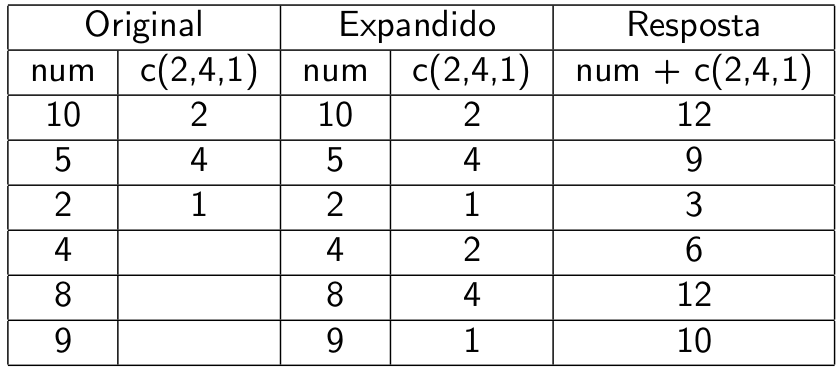
\includegraphics[width=0.8\linewidth]{img/reciclagem} \end{center}

Agora tente:

\begin{Shaded}
\begin{Highlighting}[]
\NormalTok{num }\SpecialCharTok{+} \FunctionTok{c}\NormalTok{(}\DecValTok{2}\NormalTok{, }\DecValTok{4}\NormalTok{, }\DecValTok{1}\NormalTok{, }\DecValTok{3}\NormalTok{)}
\end{Highlighting}
\end{Shaded}

\hypertarget{outros-tipos-de-vetores}{%
\subsection{Outros tipos de vetores}\label{outros-tipos-de-vetores}}

Vetores também podem ter outros tipos:

\begin{itemize}
\tightlist
\item
  Vetor de caracteres:
\end{itemize}

\begin{Shaded}
\begin{Highlighting}[]
\NormalTok{caracter }\OtherTok{\textless{}{-}} \FunctionTok{c}\NormalTok{(}\StringTok{"brava"}\NormalTok{, }\StringTok{"joaquina"}\NormalTok{, }\StringTok{"armação"}\NormalTok{)}
\NormalTok{caracter}
\NormalTok{[}\DecValTok{1}\NormalTok{] }\StringTok{"brava"}    \StringTok{"joaquina"} \StringTok{"armação"} 
\FunctionTok{typeof}\NormalTok{(caracter)}
\NormalTok{[}\DecValTok{1}\NormalTok{] }\StringTok{"character"}
\FunctionTok{class}\NormalTok{(caracter)}
\NormalTok{[}\DecValTok{1}\NormalTok{] }\StringTok{"character"}
\end{Highlighting}
\end{Shaded}

\begin{itemize}
\tightlist
\item
  Vetor lógico:
\end{itemize}

\begin{Shaded}
\begin{Highlighting}[]
\NormalTok{logico }\OtherTok{\textless{}{-}}\NormalTok{ caracter }\SpecialCharTok{==} \StringTok{"armação"}
\NormalTok{logico}
\NormalTok{[}\DecValTok{1}\NormalTok{] }\ConstantTok{FALSE} \ConstantTok{FALSE}  \ConstantTok{TRUE}
\FunctionTok{typeof}\NormalTok{(logico)}
\NormalTok{[}\DecValTok{1}\NormalTok{] }\StringTok{"logical"}
\FunctionTok{class}\NormalTok{(logico)}
\NormalTok{[}\DecValTok{1}\NormalTok{] }\StringTok{"logical"}
\end{Highlighting}
\end{Shaded}

ou

\begin{Shaded}
\begin{Highlighting}[]
\NormalTok{logico }\OtherTok{\textless{}{-}}\NormalTok{ num }\SpecialCharTok{\textgreater{}} \DecValTok{4}
\NormalTok{logico}
\NormalTok{[}\DecValTok{1}\NormalTok{]  }\ConstantTok{TRUE}  \ConstantTok{TRUE} \ConstantTok{FALSE} \ConstantTok{FALSE}  \ConstantTok{TRUE}  \ConstantTok{TRUE}
\end{Highlighting}
\end{Shaded}

No exemplo anterior, a condição \texttt{num\ \textgreater{}\ 4} é uma \textbf{expressão
condicional}, e o símbolo \texttt{\textgreater{}} um \textbf{operador lógico}. Os operadores
lógicos utilizados no R são:

\begin{longtable}[]{@{}cll@{}}
\toprule()
Operador & Sintaxe & Teste \\
\midrule()
\endhead
\texttt{\textless{}} & \texttt{a\ \textless{}\ b} & \texttt{a} é menor que \texttt{b}? \\
\texttt{\textless{}=} & \texttt{a\ \textless{}=\ b} & \texttt{a} é menor ou igual a \texttt{b}? \\
\texttt{\textgreater{}} & \texttt{a\ \textgreater{}\ b} & \texttt{a} é maior que \texttt{b} \\
\texttt{\textgreater{}=} & \texttt{a\ \textgreater{}=\ b} & \texttt{a} é maior ou igual a \texttt{b}? \\
\texttt{==} & \texttt{a\ ==\ b} & \texttt{a} é igual a \texttt{b}? \\
\texttt{!=} & \texttt{a\ !=\ b} & \texttt{a} é diferente de \texttt{b}? \\
\texttt{\%in\%} & \texttt{a\ \%in\%\ c(a,\ b)} & \texttt{a} está contido no vetor \texttt{c(a,\ b)}? \\
\bottomrule()
\end{longtable}

\hypertarget{misturando-classes-de-objetos}{%
\subsection{Misturando classes de objetos}\label{misturando-classes-de-objetos}}

Algumas vezes isso acontece por acidente, mas também pode acontecer de
propósito.

O que acontece aqui?

\begin{Shaded}
\begin{Highlighting}[]
\NormalTok{w }\OtherTok{\textless{}{-}} \FunctionTok{c}\NormalTok{(5L, }\StringTok{"a"}\NormalTok{)}
\NormalTok{x }\OtherTok{\textless{}{-}} \FunctionTok{c}\NormalTok{(}\FloatTok{1.7}\NormalTok{, }\StringTok{"a"}\NormalTok{)}
\NormalTok{y }\OtherTok{\textless{}{-}} \FunctionTok{c}\NormalTok{(}\ConstantTok{TRUE}\NormalTok{, }\DecValTok{2}\NormalTok{)}
\NormalTok{z }\OtherTok{\textless{}{-}} \FunctionTok{c}\NormalTok{(}\StringTok{"a"}\NormalTok{, T)}
\end{Highlighting}
\end{Shaded}

Lembre-se da regra:

Um vetor só pode conter elementos do mesmo tipo!

Quando objetos de diferentes tipos são misturados, ocorre a
\textbf{coerção}, para que cada elemento possua a mesma classe.

Nos exemplos acima, nós vemos o efeito da \textbf{coerção implícita}, quando
o R tenta representar todos os objetos de uma única forma.

Nós podemos forçar um objeto a mudar de classe, através da \textbf{coerção
explícita}, realizada pelas funções \texttt{as.*}:

\begin{Shaded}
\begin{Highlighting}[]
\NormalTok{x }\OtherTok{\textless{}{-}} \DecValTok{0}\SpecialCharTok{:}\DecValTok{6}
\FunctionTok{typeof}\NormalTok{(x)}
\NormalTok{[}\DecValTok{1}\NormalTok{] }\StringTok{"integer"}
\FunctionTok{class}\NormalTok{(x)}
\NormalTok{[}\DecValTok{1}\NormalTok{] }\StringTok{"integer"}
\FunctionTok{as.numeric}\NormalTok{(x)}
\NormalTok{[}\DecValTok{1}\NormalTok{] }\DecValTok{0} \DecValTok{1} \DecValTok{2} \DecValTok{3} \DecValTok{4} \DecValTok{5} \DecValTok{6}
\FunctionTok{as.logical}\NormalTok{(x)}
\NormalTok{[}\DecValTok{1}\NormalTok{] }\ConstantTok{FALSE}  \ConstantTok{TRUE}  \ConstantTok{TRUE}  \ConstantTok{TRUE}  \ConstantTok{TRUE}  \ConstantTok{TRUE}  \ConstantTok{TRUE}
\FunctionTok{as.character}\NormalTok{(x)}
\NormalTok{[}\DecValTok{1}\NormalTok{] }\StringTok{"0"} \StringTok{"1"} \StringTok{"2"} \StringTok{"3"} \StringTok{"4"} \StringTok{"5"} \StringTok{"6"}
\FunctionTok{as.factor}\NormalTok{(x)}
\NormalTok{[}\DecValTok{1}\NormalTok{] }\DecValTok{0} \DecValTok{1} \DecValTok{2} \DecValTok{3} \DecValTok{4} \DecValTok{5} \DecValTok{6}
\NormalTok{Levels}\SpecialCharTok{:} \DecValTok{0} \DecValTok{1} \DecValTok{2} \DecValTok{3} \DecValTok{4} \DecValTok{5} \DecValTok{6}
\end{Highlighting}
\end{Shaded}

De \texttt{?logical}:

\begin{verbatim}
 Logical vectors are coerced to integer vectors in contexts where a
 numerical value is required, with ‘TRUE’ being mapped to ‘1L’,
 ‘FALSE’ to ‘0L’ and ‘NA’ to ‘NA_integer_’.
\end{verbatim}

\begin{Shaded}
\begin{Highlighting}[]
\NormalTok{(x }\OtherTok{\textless{}{-}} \FunctionTok{c}\NormalTok{(}\ConstantTok{FALSE}\NormalTok{, }\ConstantTok{TRUE}\NormalTok{))}
\NormalTok{[}\DecValTok{1}\NormalTok{] }\ConstantTok{FALSE}  \ConstantTok{TRUE}
\FunctionTok{class}\NormalTok{(x)}
\NormalTok{[}\DecValTok{1}\NormalTok{] }\StringTok{"logical"}
\FunctionTok{as.numeric}\NormalTok{(x)}
\NormalTok{[}\DecValTok{1}\NormalTok{] }\DecValTok{0} \DecValTok{1}
\end{Highlighting}
\end{Shaded}

Algumas vezes não é possível fazer a coerção, então:

\begin{Shaded}
\begin{Highlighting}[]
\NormalTok{x }\OtherTok{\textless{}{-}} \FunctionTok{c}\NormalTok{(}\StringTok{"a"}\NormalTok{, }\StringTok{"b"}\NormalTok{, }\StringTok{"c"}\NormalTok{)}
\FunctionTok{as.numeric}\NormalTok{(x)}
\NormalTok{Warning}\SpecialCharTok{:}\NormalTok{ NAs introduced by coercion}
\NormalTok{[}\DecValTok{1}\NormalTok{] }\ConstantTok{NA} \ConstantTok{NA} \ConstantTok{NA}
\FunctionTok{as.logical}\NormalTok{(x)}
\NormalTok{[}\DecValTok{1}\NormalTok{] }\ConstantTok{NA} \ConstantTok{NA} \ConstantTok{NA}
\end{Highlighting}
\end{Shaded}

\hypertarget{valores-perdidos-e-especiais}{%
\subsection{Valores perdidos e especiais}\label{valores-perdidos-e-especiais}}

Valores perdidos devem ser definidos como \texttt{NA} (\emph{not available}):

\begin{Shaded}
\begin{Highlighting}[]
\NormalTok{perd }\OtherTok{\textless{}{-}} \FunctionTok{c}\NormalTok{(}\DecValTok{3}\NormalTok{, }\DecValTok{5}\NormalTok{, }\ConstantTok{NA}\NormalTok{, }\DecValTok{2}\NormalTok{)}
\NormalTok{perd}
\NormalTok{[}\DecValTok{1}\NormalTok{]  }\DecValTok{3}  \DecValTok{5} \ConstantTok{NA}  \DecValTok{2}
\FunctionTok{class}\NormalTok{(perd)}
\NormalTok{[}\DecValTok{1}\NormalTok{] }\StringTok{"numeric"}
\end{Highlighting}
\end{Shaded}

Podemos testar a presença de \texttt{NA}s com a função \texttt{is.na()}:

\begin{Shaded}
\begin{Highlighting}[]
\FunctionTok{is.na}\NormalTok{(perd)}
\NormalTok{[}\DecValTok{1}\NormalTok{] }\ConstantTok{FALSE} \ConstantTok{FALSE}  \ConstantTok{TRUE} \ConstantTok{FALSE}
\end{Highlighting}
\end{Shaded}

Ou:

\begin{Shaded}
\begin{Highlighting}[]
\FunctionTok{any}\NormalTok{(}\FunctionTok{is.na}\NormalTok{(perd))}
\NormalTok{[}\DecValTok{1}\NormalTok{] }\ConstantTok{TRUE}
\end{Highlighting}
\end{Shaded}

Outros valores especiais são:

\begin{itemize}
\tightlist
\item
  \texttt{NaN} (\emph{not a number}) - exemplo: \texttt{0/0}
\item
  \texttt{-Inf} e \texttt{Inf} - exemplo: \texttt{1/0}
\end{itemize}

A função \texttt{is.na()} também testa a presença de \texttt{NaN}s:

\begin{Shaded}
\begin{Highlighting}[]
\NormalTok{perd }\OtherTok{\textless{}{-}} \FunctionTok{c}\NormalTok{(}\SpecialCharTok{{-}}\DecValTok{1}\NormalTok{,}\DecValTok{0}\NormalTok{,}\DecValTok{1}\NormalTok{)}\SpecialCharTok{/}\DecValTok{0}
\NormalTok{perd}
\NormalTok{[}\DecValTok{1}\NormalTok{] }\SpecialCharTok{{-}}\ConstantTok{Inf}  \ConstantTok{NaN}  \ConstantTok{Inf}
\FunctionTok{is.na}\NormalTok{(perd)}
\NormalTok{[}\DecValTok{1}\NormalTok{] }\ConstantTok{FALSE}  \ConstantTok{TRUE} \ConstantTok{FALSE}
\end{Highlighting}
\end{Shaded}

A função \texttt{is.infinite()} testa se há valores infinitos

\begin{Shaded}
\begin{Highlighting}[]
\FunctionTok{is.infinite}\NormalTok{(perd)}
\NormalTok{[}\DecValTok{1}\NormalTok{]  }\ConstantTok{TRUE} \ConstantTok{FALSE}  \ConstantTok{TRUE}
\end{Highlighting}
\end{Shaded}

\hypertarget{exercuxedcios-3}{%
\section*{Exercícios}\label{exercuxedcios-3}}


\begin{enumerate}
\def\labelenumi{\arabic{enumi}.}
\tightlist
\item
  Crie um objeto com os valores 54, 0, 17, 94, 12.5, 2, 0.9, 15.

  \begin{enumerate}
  \def\labelenumii{\alph{enumii}.}
  \tightlist
  \item
    Some o objeto acima com os valores 5, 6, e depois com os valores 5,
    6, 7.
  \end{enumerate}
\item
  Construa um único objeto com as letras: \texttt{A}, \texttt{B}, e \texttt{C}, repetidas
  cada uma 15, 12, e 8 vezes, respectivamente.

  \begin{enumerate}
  \def\labelenumii{\alph{enumii}.}
  \tightlist
  \item
    Mostre na tela, em forma de verdadeiro ou falso, onde estão as letras
    \texttt{B} nesse objeto.
  \item
    Veja a página de ajuda da função \texttt{sum()} e descubra como fazer para
    contar o número de letras \texttt{B} neste vetor (usando \texttt{sum()}).
  \end{enumerate}
\item
  Crie um objeto com 100 valores aleatórios de uma distribuição uniforme
  \(U(0,1)\). Conte quantas vezes aparecem valores maiores ou iguais a 0,5.
\item
  Calcule as 50 primeiras potências de 2, ou seja, \(2, 2^2, 2^3, \ldots, 2^{50}\).

  \begin{enumerate}
  \def\labelenumii{\alph{enumii}.}
  \tightlist
  \item
    Calcule o quadrado dos números inteiros de 1 a 50, ou seja, \(1^2,  2^2, 3^2, \ldots, 50^2\).
  \item
    Quais pares são iguais, ou seja, quais números inteiros dos dois
    exercícios anteriores satisfazem a condição \(2^n = n^2\)?
  \item
    Quantos pares existem?
  \end{enumerate}
\item
  Calcule o seno, coseno e a tangente para os números variando de \(0\) a
  \(2\pi\), com distância de \(0.1\) entre eles. (Use as funções \texttt{sin()},
  \texttt{cos()}, \texttt{tan()}).

  \begin{enumerate}
  \def\labelenumii{\alph{enumii}.}
  \tightlist
  \item
    Calcule a tangente usando a relação \(\tan(x) = \sin(x)/\cos(x)\).
  \item
    Calcule as diferenças das tangentes calculadas pela função do R e
    pela razão acima.
  \item
    Quais valores são exatamente iguais?
  \item
    Qual a diferença máxima (em módulo) entre eles? Qual é a causa
    dessa diferença?
  \end{enumerate}
\end{enumerate}

\hypertarget{outras-classes}{%
\section{Outras classes}\label{outras-classes}}

Como mencionado na seção anterior, o R possui 6 tipos básicos de
estrutura de dados, mas diversas classes podem ser construídas a partir
destes tipos básicos. Abaixo, veremos algumas das mais importantes.

\hypertarget{fator}{%
\subsection{Fator}\label{fator}}

Os fatores são parecidos com caracteres no R, mas são armazenados e
tratados de maneira diferente.

Características:

\begin{itemize}
\tightlist
\item
  Coleção de categorias ou \textbf{níveis} (\emph{levels}).
\item
  Estrutura unidimensional.
\end{itemize}

Utilizando as funções \texttt{factor()} e \texttt{c()}:

\begin{Shaded}
\begin{Highlighting}[]
\NormalTok{fator }\OtherTok{\textless{}{-}} \FunctionTok{factor}\NormalTok{(}\FunctionTok{c}\NormalTok{(}\StringTok{"alta"}\NormalTok{,}\StringTok{"baixa"}\NormalTok{,}\StringTok{"baixa"}\NormalTok{,}\StringTok{"media"}\NormalTok{,}
                  \StringTok{"alta"}\NormalTok{,}\StringTok{"media"}\NormalTok{,}\StringTok{"baixa"}\NormalTok{,}\StringTok{"media"}\NormalTok{,}\StringTok{"media"}\NormalTok{))}
\NormalTok{fator}
\NormalTok{[}\DecValTok{1}\NormalTok{] alta  baixa baixa media alta  media baixa media media}
\NormalTok{Levels}\SpecialCharTok{:}\NormalTok{ alta baixa media}
\FunctionTok{class}\NormalTok{(fator)}
\NormalTok{[}\DecValTok{1}\NormalTok{] }\StringTok{"factor"}
\FunctionTok{typeof}\NormalTok{(fator)}
\NormalTok{[}\DecValTok{1}\NormalTok{] }\StringTok{"integer"}
\end{Highlighting}
\end{Shaded}

Note que o objeto é da classe \texttt{factor}, mas seu tipo básico é \texttt{integer}!
Isso significa que cada categoria única é identificada internamente por
um número, e isso faz com que os fatores possuam uma ordenação, de
acordo com as categorias únicas. Por isso existe a identificação dos
\texttt{Levels} (níveis) de um fator.

Veja o que acontece quando ``remover a classe'' desse objeto

\begin{Shaded}
\begin{Highlighting}[]
\FunctionTok{unclass}\NormalTok{(fator)}
\NormalTok{[}\DecValTok{1}\NormalTok{] }\DecValTok{1} \DecValTok{2} \DecValTok{2} \DecValTok{3} \DecValTok{1} \DecValTok{3} \DecValTok{2} \DecValTok{3} \DecValTok{3}
\FunctionTok{attr}\NormalTok{(,}\StringTok{"levels"}\NormalTok{)}
\NormalTok{[}\DecValTok{1}\NormalTok{] }\StringTok{"alta"}  \StringTok{"baixa"} \StringTok{"media"}
\end{Highlighting}
\end{Shaded}

Fatores podem ser convertidos para caracteres, e \textbf{também} para números
inteiros

\begin{Shaded}
\begin{Highlighting}[]
\FunctionTok{as.character}\NormalTok{(fator)}
\NormalTok{[}\DecValTok{1}\NormalTok{] }\StringTok{"alta"}  \StringTok{"baixa"} \StringTok{"baixa"} \StringTok{"media"} \StringTok{"alta"}  \StringTok{"media"} \StringTok{"baixa"} \StringTok{"media"} \StringTok{"media"}
\FunctionTok{as.integer}\NormalTok{(fator)}
\NormalTok{[}\DecValTok{1}\NormalTok{] }\DecValTok{1} \DecValTok{2} \DecValTok{2} \DecValTok{3} \DecValTok{1} \DecValTok{3} \DecValTok{2} \DecValTok{3} \DecValTok{3}
\end{Highlighting}
\end{Shaded}

Caso haja uma hierarquia, os níveis dos fatores podem ser ordenados
explicitamente através do argumento \texttt{levels}:

\begin{Shaded}
\begin{Highlighting}[]
\NormalTok{fator }\OtherTok{\textless{}{-}} \FunctionTok{factor}\NormalTok{(}\FunctionTok{c}\NormalTok{(}\StringTok{"alta"}\NormalTok{,}\StringTok{"baixa"}\NormalTok{,}\StringTok{"baixa"}\NormalTok{,}\StringTok{"media"}\NormalTok{,}
                  \StringTok{"alta"}\NormalTok{,}\StringTok{"media"}\NormalTok{,}\StringTok{"baixa"}\NormalTok{,}\StringTok{"media"}\NormalTok{,}\StringTok{"media"}\NormalTok{),}
                \AttributeTok{levels =} \FunctionTok{c}\NormalTok{(}\StringTok{"alta"}\NormalTok{,}\StringTok{"media"}\NormalTok{,}\StringTok{"baixa"}\NormalTok{))}
\NormalTok{fator}
\NormalTok{[}\DecValTok{1}\NormalTok{] alta  baixa baixa media alta  media baixa media media}
\NormalTok{Levels}\SpecialCharTok{:}\NormalTok{ alta media baixa}
\FunctionTok{typeof}\NormalTok{(fator)}
\NormalTok{[}\DecValTok{1}\NormalTok{] }\StringTok{"integer"}
\FunctionTok{class}\NormalTok{(fator)}
\NormalTok{[}\DecValTok{1}\NormalTok{] }\StringTok{"factor"}
\end{Highlighting}
\end{Shaded}

Além disso, os níveis dos fatores podem também ser explicitamente
ordenados

\begin{Shaded}
\begin{Highlighting}[]
\NormalTok{fator }\OtherTok{\textless{}{-}} \FunctionTok{factor}\NormalTok{(}\FunctionTok{c}\NormalTok{(}\StringTok{"alta"}\NormalTok{,}\StringTok{"baixa"}\NormalTok{,}\StringTok{"baixa"}\NormalTok{,}\StringTok{"media"}\NormalTok{,}
                  \StringTok{"alta"}\NormalTok{,}\StringTok{"media"}\NormalTok{,}\StringTok{"baixa"}\NormalTok{,}\StringTok{"media"}\NormalTok{,}\StringTok{"media"}\NormalTok{),}
                \AttributeTok{levels =} \FunctionTok{c}\NormalTok{(}\StringTok{"baixa"}\NormalTok{, }\StringTok{"media"}\NormalTok{, }\StringTok{"alta"}\NormalTok{),}
                \AttributeTok{ordered =} \ConstantTok{TRUE}\NormalTok{)}
\NormalTok{fator}
\NormalTok{[}\DecValTok{1}\NormalTok{] alta  baixa baixa media alta  media baixa media media}
\NormalTok{Levels}\SpecialCharTok{:}\NormalTok{ baixa }\SpecialCharTok{\textless{}}\NormalTok{ media }\SpecialCharTok{\textless{}}\NormalTok{ alta}
\FunctionTok{typeof}\NormalTok{(fator)}
\NormalTok{[}\DecValTok{1}\NormalTok{] }\StringTok{"integer"}
\FunctionTok{class}\NormalTok{(fator)}
\NormalTok{[}\DecValTok{1}\NormalTok{] }\StringTok{"ordered"} \StringTok{"factor"} 
\end{Highlighting}
\end{Shaded}

Veja que um objeto pode ter mais de uma classe. Isso geralmente só
será útil em casos especificos.

As seguintes funções são úteis para verificar os níveis e o número de
níveis de um fator:

\begin{Shaded}
\begin{Highlighting}[]
\FunctionTok{levels}\NormalTok{(fator)}
\NormalTok{[}\DecValTok{1}\NormalTok{] }\StringTok{"baixa"} \StringTok{"media"} \StringTok{"alta"} 
\FunctionTok{nlevels}\NormalTok{(fator)}
\NormalTok{[}\DecValTok{1}\NormalTok{] }\DecValTok{3}
\end{Highlighting}
\end{Shaded}

\hypertarget{matriz}{%
\subsection{Matriz}\label{matriz}}

Matrizes são vetores que podem ser dispostos em duas dimensões.

Características:

\begin{itemize}
\tightlist
\item
  Podem conter apenas um tipo de informação (números, caracteres)
\item
  Estrutura bidimensional
\end{itemize}

Utilizando a função \texttt{matrix()}:

\begin{Shaded}
\begin{Highlighting}[]
\NormalTok{matriz }\OtherTok{\textless{}{-}} \FunctionTok{matrix}\NormalTok{(}\DecValTok{1}\SpecialCharTok{:}\DecValTok{12}\NormalTok{, }\AttributeTok{nrow =} \DecValTok{3}\NormalTok{, }\AttributeTok{ncol =} \DecValTok{4}\NormalTok{)}
\NormalTok{matriz}
\NormalTok{     [,}\DecValTok{1}\NormalTok{] [,}\DecValTok{2}\NormalTok{] [,}\DecValTok{3}\NormalTok{] [,}\DecValTok{4}\NormalTok{]}
\NormalTok{[}\DecValTok{1}\NormalTok{,]    }\DecValTok{1}    \DecValTok{4}    \DecValTok{7}   \DecValTok{10}
\NormalTok{[}\DecValTok{2}\NormalTok{,]    }\DecValTok{2}    \DecValTok{5}    \DecValTok{8}   \DecValTok{11}
\NormalTok{[}\DecValTok{3}\NormalTok{,]    }\DecValTok{3}    \DecValTok{6}    \DecValTok{9}   \DecValTok{12}
\FunctionTok{class}\NormalTok{(matriz)}
\NormalTok{[}\DecValTok{1}\NormalTok{] }\StringTok{"matrix"} \StringTok{"array"} 
\FunctionTok{typeof}\NormalTok{(matriz)}
\NormalTok{[}\DecValTok{1}\NormalTok{] }\StringTok{"integer"}
\end{Highlighting}
\end{Shaded}

Alterando a ordem de preenchimento da matriz (por linhas):

\begin{Shaded}
\begin{Highlighting}[]
\NormalTok{matriz }\OtherTok{\textless{}{-}} \FunctionTok{matrix}\NormalTok{(}\DecValTok{1}\SpecialCharTok{:}\DecValTok{12}\NormalTok{, }\AttributeTok{nrow =} \DecValTok{3}\NormalTok{, }\AttributeTok{ncol =} \DecValTok{4}\NormalTok{, }\AttributeTok{byrow =} \ConstantTok{TRUE}\NormalTok{)}
\NormalTok{matriz}
\NormalTok{     [,}\DecValTok{1}\NormalTok{] [,}\DecValTok{2}\NormalTok{] [,}\DecValTok{3}\NormalTok{] [,}\DecValTok{4}\NormalTok{]}
\NormalTok{[}\DecValTok{1}\NormalTok{,]    }\DecValTok{1}    \DecValTok{2}    \DecValTok{3}    \DecValTok{4}
\NormalTok{[}\DecValTok{2}\NormalTok{,]    }\DecValTok{5}    \DecValTok{6}    \DecValTok{7}    \DecValTok{8}
\NormalTok{[}\DecValTok{3}\NormalTok{,]    }\DecValTok{9}   \DecValTok{10}   \DecValTok{11}   \DecValTok{12}
\end{Highlighting}
\end{Shaded}

Para verificar a dimensão da matriz:

\begin{Shaded}
\begin{Highlighting}[]
\FunctionTok{dim}\NormalTok{(matriz)}
\NormalTok{[}\DecValTok{1}\NormalTok{] }\DecValTok{3} \DecValTok{4}
\end{Highlighting}
\end{Shaded}

Adicionando colunas com \texttt{cbind()}

\begin{Shaded}
\begin{Highlighting}[]
\FunctionTok{cbind}\NormalTok{(matriz, }\FunctionTok{rep}\NormalTok{(}\DecValTok{99}\NormalTok{, }\DecValTok{3}\NormalTok{))}
\NormalTok{     [,}\DecValTok{1}\NormalTok{] [,}\DecValTok{2}\NormalTok{] [,}\DecValTok{3}\NormalTok{] [,}\DecValTok{4}\NormalTok{] [,}\DecValTok{5}\NormalTok{]}
\NormalTok{[}\DecValTok{1}\NormalTok{,]    }\DecValTok{1}    \DecValTok{2}    \DecValTok{3}    \DecValTok{4}   \DecValTok{99}
\NormalTok{[}\DecValTok{2}\NormalTok{,]    }\DecValTok{5}    \DecValTok{6}    \DecValTok{7}    \DecValTok{8}   \DecValTok{99}
\NormalTok{[}\DecValTok{3}\NormalTok{,]    }\DecValTok{9}   \DecValTok{10}   \DecValTok{11}   \DecValTok{12}   \DecValTok{99}
\end{Highlighting}
\end{Shaded}

Adicionando linhas com \texttt{rbind()}

\begin{Shaded}
\begin{Highlighting}[]
\FunctionTok{rbind}\NormalTok{(matriz, }\FunctionTok{rep}\NormalTok{(}\DecValTok{99}\NormalTok{, }\DecValTok{4}\NormalTok{))}
\NormalTok{     [,}\DecValTok{1}\NormalTok{] [,}\DecValTok{2}\NormalTok{] [,}\DecValTok{3}\NormalTok{] [,}\DecValTok{4}\NormalTok{]}
\NormalTok{[}\DecValTok{1}\NormalTok{,]    }\DecValTok{1}    \DecValTok{2}    \DecValTok{3}    \DecValTok{4}
\NormalTok{[}\DecValTok{2}\NormalTok{,]    }\DecValTok{5}    \DecValTok{6}    \DecValTok{7}    \DecValTok{8}
\NormalTok{[}\DecValTok{3}\NormalTok{,]    }\DecValTok{9}   \DecValTok{10}   \DecValTok{11}   \DecValTok{12}
\NormalTok{[}\DecValTok{4}\NormalTok{,]   }\DecValTok{99}   \DecValTok{99}   \DecValTok{99}   \DecValTok{99}
\end{Highlighting}
\end{Shaded}

Matrizes também podem ser criadas a partir de vetores adicionando um
\textbf{atributo} de dimensão, por exemplo,

\begin{Shaded}
\begin{Highlighting}[]
\NormalTok{m }\OtherTok{\textless{}{-}} \DecValTok{1}\SpecialCharTok{:}\DecValTok{10}
\NormalTok{m}
\NormalTok{ [}\DecValTok{1}\NormalTok{]  }\DecValTok{1}  \DecValTok{2}  \DecValTok{3}  \DecValTok{4}  \DecValTok{5}  \DecValTok{6}  \DecValTok{7}  \DecValTok{8}  \DecValTok{9} \DecValTok{10}
\FunctionTok{class}\NormalTok{(m)}
\NormalTok{[}\DecValTok{1}\NormalTok{] }\StringTok{"integer"}
\FunctionTok{dim}\NormalTok{(m)}
\ConstantTok{NULL}
\FunctionTok{dim}\NormalTok{(m) }\OtherTok{\textless{}{-}} \FunctionTok{c}\NormalTok{(}\DecValTok{2}\NormalTok{, }\DecValTok{5}\NormalTok{)}
\NormalTok{m}
\NormalTok{     [,}\DecValTok{1}\NormalTok{] [,}\DecValTok{2}\NormalTok{] [,}\DecValTok{3}\NormalTok{] [,}\DecValTok{4}\NormalTok{] [,}\DecValTok{5}\NormalTok{]}
\NormalTok{[}\DecValTok{1}\NormalTok{,]    }\DecValTok{1}    \DecValTok{3}    \DecValTok{5}    \DecValTok{7}    \DecValTok{9}
\NormalTok{[}\DecValTok{2}\NormalTok{,]    }\DecValTok{2}    \DecValTok{4}    \DecValTok{6}    \DecValTok{8}   \DecValTok{10}
\FunctionTok{class}\NormalTok{(m)}
\NormalTok{[}\DecValTok{1}\NormalTok{] }\StringTok{"matrix"} \StringTok{"array"} 
\FunctionTok{typeof}\NormalTok{(m)}
\NormalTok{[}\DecValTok{1}\NormalTok{] }\StringTok{"integer"}
\end{Highlighting}
\end{Shaded}

\hypertarget{operauxe7uxf5es-matemuxe1ticas-em-matrizes}{%
\subsubsection{Operações matemáticas em matrizes}\label{operauxe7uxf5es-matemuxe1ticas-em-matrizes}}

Matriz multiplicada por um escalar

\begin{Shaded}
\begin{Highlighting}[]
\NormalTok{matriz }\SpecialCharTok{*} \DecValTok{2}
\NormalTok{     [,}\DecValTok{1}\NormalTok{] [,}\DecValTok{2}\NormalTok{] [,}\DecValTok{3}\NormalTok{] [,}\DecValTok{4}\NormalTok{]}
\NormalTok{[}\DecValTok{1}\NormalTok{,]    }\DecValTok{2}    \DecValTok{4}    \DecValTok{6}    \DecValTok{8}
\NormalTok{[}\DecValTok{2}\NormalTok{,]   }\DecValTok{10}   \DecValTok{12}   \DecValTok{14}   \DecValTok{16}
\NormalTok{[}\DecValTok{3}\NormalTok{,]   }\DecValTok{18}   \DecValTok{20}   \DecValTok{22}   \DecValTok{24}
\end{Highlighting}
\end{Shaded}

Multiplicação de matrizes (observe as dimensões!)

\begin{Shaded}
\begin{Highlighting}[]
\NormalTok{matriz2 }\OtherTok{\textless{}{-}} \FunctionTok{matrix}\NormalTok{(}\DecValTok{1}\NormalTok{, }\AttributeTok{nrow =} \DecValTok{4}\NormalTok{, }\AttributeTok{ncol =} \DecValTok{3}\NormalTok{)}
\NormalTok{matriz }\SpecialCharTok{\%*\%}\NormalTok{ matriz2}
\NormalTok{     [,}\DecValTok{1}\NormalTok{] [,}\DecValTok{2}\NormalTok{] [,}\DecValTok{3}\NormalTok{]}
\NormalTok{[}\DecValTok{1}\NormalTok{,]   }\DecValTok{10}   \DecValTok{10}   \DecValTok{10}
\NormalTok{[}\DecValTok{2}\NormalTok{,]   }\DecValTok{26}   \DecValTok{26}   \DecValTok{26}
\NormalTok{[}\DecValTok{3}\NormalTok{,]   }\DecValTok{42}   \DecValTok{42}   \DecValTok{42}
\end{Highlighting}
\end{Shaded}

\hypertarget{array}{%
\subsection{Array}\label{array}}

Um array é a forma mais geral de uma matriz, pois pode ter \(n\)
dimensões.

Características:

\begin{itemize}
\tightlist
\item
  Estrutura \(n\)-dimensional.
\item
  Assim como as matrizes, podem conter apenas um tipo de informação
  (números, caracteres).
\end{itemize}

Para criar um array, usamos a função \texttt{array()}, passando como primeiro
argumento um vetor atômico, e especificamos a dimensão com o argumento
\texttt{dim}. Por exemplo, para criar um objeto com 3 dimensões \(2 \times 2 \times 3\), fazemos

\begin{Shaded}
\begin{Highlighting}[]
\NormalTok{ar }\OtherTok{\textless{}{-}} \FunctionTok{array}\NormalTok{(}\DecValTok{1}\SpecialCharTok{:}\DecValTok{12}\NormalTok{, }\AttributeTok{dim =} \FunctionTok{c}\NormalTok{(}\DecValTok{2}\NormalTok{, }\DecValTok{2}\NormalTok{, }\DecValTok{3}\NormalTok{))}
\NormalTok{ar}
\NormalTok{, , }\DecValTok{1}

\NormalTok{     [,}\DecValTok{1}\NormalTok{] [,}\DecValTok{2}\NormalTok{]}
\NormalTok{[}\DecValTok{1}\NormalTok{,]    }\DecValTok{1}    \DecValTok{3}
\NormalTok{[}\DecValTok{2}\NormalTok{,]    }\DecValTok{2}    \DecValTok{4}

\NormalTok{, , }\DecValTok{2}

\NormalTok{     [,}\DecValTok{1}\NormalTok{] [,}\DecValTok{2}\NormalTok{]}
\NormalTok{[}\DecValTok{1}\NormalTok{,]    }\DecValTok{5}    \DecValTok{7}
\NormalTok{[}\DecValTok{2}\NormalTok{,]    }\DecValTok{6}    \DecValTok{8}

\NormalTok{, , }\DecValTok{3}

\NormalTok{     [,}\DecValTok{1}\NormalTok{] [,}\DecValTok{2}\NormalTok{]}
\NormalTok{[}\DecValTok{1}\NormalTok{,]    }\DecValTok{9}   \DecValTok{11}
\NormalTok{[}\DecValTok{2}\NormalTok{,]   }\DecValTok{10}   \DecValTok{12}
\end{Highlighting}
\end{Shaded}

Similarmente, um array de 2 dimensões \(3 \times 2 \times 2\) é obtido com

\begin{Shaded}
\begin{Highlighting}[]
\NormalTok{ar }\OtherTok{\textless{}{-}} \FunctionTok{array}\NormalTok{(}\DecValTok{1}\SpecialCharTok{:}\DecValTok{12}\NormalTok{, }\AttributeTok{dim =} \FunctionTok{c}\NormalTok{(}\DecValTok{3}\NormalTok{, }\DecValTok{2}\NormalTok{, }\DecValTok{2}\NormalTok{))}
\NormalTok{ar}
\NormalTok{, , }\DecValTok{1}

\NormalTok{     [,}\DecValTok{1}\NormalTok{] [,}\DecValTok{2}\NormalTok{]}
\NormalTok{[}\DecValTok{1}\NormalTok{,]    }\DecValTok{1}    \DecValTok{4}
\NormalTok{[}\DecValTok{2}\NormalTok{,]    }\DecValTok{2}    \DecValTok{5}
\NormalTok{[}\DecValTok{3}\NormalTok{,]    }\DecValTok{3}    \DecValTok{6}

\NormalTok{, , }\DecValTok{2}

\NormalTok{     [,}\DecValTok{1}\NormalTok{] [,}\DecValTok{2}\NormalTok{]}
\NormalTok{[}\DecValTok{1}\NormalTok{,]    }\DecValTok{7}   \DecValTok{10}
\NormalTok{[}\DecValTok{2}\NormalTok{,]    }\DecValTok{8}   \DecValTok{11}
\NormalTok{[}\DecValTok{3}\NormalTok{,]    }\DecValTok{9}   \DecValTok{12}
\end{Highlighting}
\end{Shaded}

\hypertarget{lista}{%
\subsection{Lista}\label{lista}}

Como já vimos, uma lista não é uma ``classe'' propriamente dita, mas sim
um tipo de estrutura de dados básico, ao lado dos vetores atômicos. E,
assim como os vetores atômicos, listas são estruturas unidimensionais. A
grande diferença é que listas agrupam objetos de diferentes tipos,
inclusive outras listas.

Características:

\begin{itemize}
\tightlist
\item
  Pode combinar uma coleção de objetos de diferentes tipos ou classes (é
  um tipo básico de vetor, assim como os vetores atômicos).
\item
  Estrutura ``unidimensional'': apenas o número de elementos na lista é
  contado.
\end{itemize}

Por exemplo, podemos criar uma lista com uma sequência de números, um
caracter e outra lista.

\begin{Shaded}
\begin{Highlighting}[]
\NormalTok{lista }\OtherTok{\textless{}{-}} \FunctionTok{list}\NormalTok{(}\DecValTok{1}\SpecialCharTok{:}\DecValTok{30}\NormalTok{, }\StringTok{"R"}\NormalTok{, }\FunctionTok{list}\NormalTok{(}\ConstantTok{TRUE}\NormalTok{, }\ConstantTok{FALSE}\NormalTok{))}
\NormalTok{lista}
\NormalTok{[[}\DecValTok{1}\NormalTok{]]}
\NormalTok{ [}\DecValTok{1}\NormalTok{]  }\DecValTok{1}  \DecValTok{2}  \DecValTok{3}  \DecValTok{4}  \DecValTok{5}  \DecValTok{6}  \DecValTok{7}  \DecValTok{8}  \DecValTok{9} \DecValTok{10} \DecValTok{11} \DecValTok{12} \DecValTok{13} \DecValTok{14} \DecValTok{15} \DecValTok{16} \DecValTok{17} \DecValTok{18} \DecValTok{19} \DecValTok{20} \DecValTok{21} \DecValTok{22} \DecValTok{23} \DecValTok{24} \DecValTok{25}
\NormalTok{[}\DecValTok{26}\NormalTok{] }\DecValTok{26} \DecValTok{27} \DecValTok{28} \DecValTok{29} \DecValTok{30}

\NormalTok{[[}\DecValTok{2}\NormalTok{]]}
\NormalTok{[}\DecValTok{1}\NormalTok{] }\StringTok{"R"}

\NormalTok{[[}\DecValTok{3}\NormalTok{]]}
\NormalTok{[[}\DecValTok{3}\NormalTok{]][[}\DecValTok{1}\NormalTok{]]}
\NormalTok{[}\DecValTok{1}\NormalTok{] }\ConstantTok{TRUE}

\NormalTok{[[}\DecValTok{3}\NormalTok{]][[}\DecValTok{2}\NormalTok{]]}
\NormalTok{[}\DecValTok{1}\NormalTok{] }\ConstantTok{FALSE}
\FunctionTok{class}\NormalTok{(lista)}
\NormalTok{[}\DecValTok{1}\NormalTok{] }\StringTok{"list"}
\FunctionTok{typeof}\NormalTok{(lista)}
\NormalTok{[}\DecValTok{1}\NormalTok{] }\StringTok{"list"}
\end{Highlighting}
\end{Shaded}

Para melhor visualizar a estrutura dessa lista (ou de qualquer outro
objeto) podemos usar a função \texttt{str()}

\begin{Shaded}
\begin{Highlighting}[]
\FunctionTok{str}\NormalTok{(lista)}
\NormalTok{List of }\DecValTok{3}
 \SpecialCharTok{$} \ErrorTok{:}\NormalTok{ int [}\DecValTok{1}\SpecialCharTok{:}\DecValTok{30}\NormalTok{] }\DecValTok{1} \DecValTok{2} \DecValTok{3} \DecValTok{4} \DecValTok{5} \DecValTok{6} \DecValTok{7} \DecValTok{8} \DecValTok{9} \DecValTok{10}\NormalTok{ ...}
 \SpecialCharTok{$} \ErrorTok{:}\NormalTok{ chr }\StringTok{"R"}
 \SpecialCharTok{$} \ErrorTok{:}\NormalTok{List of }\DecValTok{2}
\NormalTok{  ..}\SpecialCharTok{$} \ErrorTok{:}\NormalTok{ logi }\ConstantTok{TRUE}
\NormalTok{  ..}\SpecialCharTok{$} \ErrorTok{:}\NormalTok{ logi }\ConstantTok{FALSE}
\end{Highlighting}
\end{Shaded}

Note que de fato é uma estrutura unidimensional

\begin{Shaded}
\begin{Highlighting}[]
\FunctionTok{dim}\NormalTok{(lista)}
\ConstantTok{NULL}
\FunctionTok{length}\NormalTok{(lista)}
\NormalTok{[}\DecValTok{1}\NormalTok{] }\DecValTok{3}
\end{Highlighting}
\end{Shaded}

Listas podem armazenar objetos de diferentes classes e dimensões, por
exemplo, usando objetos criados anteriormente

\begin{Shaded}
\begin{Highlighting}[]
\NormalTok{lista }\OtherTok{\textless{}{-}} \FunctionTok{list}\NormalTok{(fator, matriz)}
\NormalTok{lista}
\NormalTok{[[}\DecValTok{1}\NormalTok{]]}
\NormalTok{[}\DecValTok{1}\NormalTok{] alta  baixa baixa media alta  media baixa media media}
\NormalTok{Levels}\SpecialCharTok{:}\NormalTok{ baixa }\SpecialCharTok{\textless{}}\NormalTok{ media }\SpecialCharTok{\textless{}}\NormalTok{ alta}

\NormalTok{[[}\DecValTok{2}\NormalTok{]]}
\NormalTok{     [,}\DecValTok{1}\NormalTok{] [,}\DecValTok{2}\NormalTok{] [,}\DecValTok{3}\NormalTok{] [,}\DecValTok{4}\NormalTok{]}
\NormalTok{[}\DecValTok{1}\NormalTok{,]    }\DecValTok{1}    \DecValTok{2}    \DecValTok{3}    \DecValTok{4}
\NormalTok{[}\DecValTok{2}\NormalTok{,]    }\DecValTok{5}    \DecValTok{6}    \DecValTok{7}    \DecValTok{8}
\NormalTok{[}\DecValTok{3}\NormalTok{,]    }\DecValTok{9}   \DecValTok{10}   \DecValTok{11}   \DecValTok{12}
\FunctionTok{length}\NormalTok{(lista)}
\NormalTok{[}\DecValTok{1}\NormalTok{] }\DecValTok{2}
\end{Highlighting}
\end{Shaded}

\hypertarget{data-frame}{%
\subsection{Data frame}\label{data-frame}}

Data frame é a versão bidimensional de uma lista. Data frames \textbf{são}
listas, mas onde cada componente deve ter obrigatoriamente o mesmo
comprimento. Cada vetor da lista vira uma coluna em um data frame,
permitindo então que as ``colunas'' sejam de diferentes tipos.

Os data frames são as estruturas mais comuns para se trabalhar com dados
no R.

Características:

\begin{itemize}
\tightlist
\item
  Uma lista de vetores e/ou fatores, de \textbf{mesmo comprimento}.
\item
  Pode conter diferentes tipos de dados (numérico, fator, \ldots).
\item
  Estrutura bidimensional.
\end{itemize}

Utilizando a função \texttt{data.frame()}:

\begin{Shaded}
\begin{Highlighting}[]
\NormalTok{da }\OtherTok{\textless{}{-}} \FunctionTok{data.frame}\NormalTok{(}\AttributeTok{nome =} \FunctionTok{c}\NormalTok{(}\StringTok{"João"}\NormalTok{, }\StringTok{"José"}\NormalTok{, }\StringTok{"Maria"}\NormalTok{),}
                 \AttributeTok{sexo =} \FunctionTok{c}\NormalTok{(}\StringTok{"M"}\NormalTok{, }\StringTok{"M"}\NormalTok{, }\StringTok{"F"}\NormalTok{),}
                 \AttributeTok{idade =} \FunctionTok{c}\NormalTok{(}\DecValTok{32}\NormalTok{, }\DecValTok{34}\NormalTok{, }\DecValTok{30}\NormalTok{))}
\NormalTok{da}
\NormalTok{   nome sexo idade}
\DecValTok{1}\NormalTok{  João    M    }\DecValTok{32}
\DecValTok{2}\NormalTok{  José    M    }\DecValTok{34}
\DecValTok{3}\NormalTok{ Maria    F    }\DecValTok{30}
\FunctionTok{class}\NormalTok{(da)}
\NormalTok{[}\DecValTok{1}\NormalTok{] }\StringTok{"data.frame"}
\FunctionTok{typeof}\NormalTok{(da)}
\NormalTok{[}\DecValTok{1}\NormalTok{] }\StringTok{"list"}
\FunctionTok{dim}\NormalTok{(da)}
\NormalTok{[}\DecValTok{1}\NormalTok{] }\DecValTok{3} \DecValTok{3}
\end{Highlighting}
\end{Shaded}

Veja os detalhes com \texttt{str()}

\begin{Shaded}
\begin{Highlighting}[]
\FunctionTok{str}\NormalTok{(da)}
\StringTok{\textquotesingle{}data.frame\textquotesingle{}}\SpecialCharTok{:}   \DecValTok{3}\NormalTok{ obs. of  }\DecValTok{3}\NormalTok{ variables}\SpecialCharTok{:}
 \ErrorTok{$}\NormalTok{ nome }\SpecialCharTok{:}\NormalTok{ chr  }\StringTok{"João"} \StringTok{"José"} \StringTok{"Maria"}
 \SpecialCharTok{$}\NormalTok{ sexo }\SpecialCharTok{:}\NormalTok{ chr  }\StringTok{"M"} \StringTok{"M"} \StringTok{"F"}
 \SpecialCharTok{$}\NormalTok{ idade}\SpecialCharTok{:}\NormalTok{ num  }\DecValTok{32} \DecValTok{34} \DecValTok{30}
\end{Highlighting}
\end{Shaded}

Em versões anteriores a função \texttt{data.frame()} convertia caracteres para fator
automaticamente mas o padrão mudou. Use o argumento \texttt{stringsAsFactors} para controlar este comportamento.

\begin{Shaded}
\begin{Highlighting}[]
\NormalTok{da }\OtherTok{\textless{}{-}} \FunctionTok{data.frame}\NormalTok{(}\AttributeTok{nome =} \FunctionTok{c}\NormalTok{(}\StringTok{"João"}\NormalTok{, }\StringTok{"José"}\NormalTok{, }\StringTok{"Maria"}\NormalTok{),}
                 \AttributeTok{sexo =} \FunctionTok{c}\NormalTok{(}\StringTok{"M"}\NormalTok{, }\StringTok{"M"}\NormalTok{, }\StringTok{"F"}\NormalTok{),}
                 \AttributeTok{idade =} \FunctionTok{c}\NormalTok{(}\DecValTok{32}\NormalTok{, }\DecValTok{34}\NormalTok{, }\DecValTok{30}\NormalTok{))}
\NormalTok{da }
\NormalTok{   nome sexo idade}
\DecValTok{1}\NormalTok{  João    M    }\DecValTok{32}
\DecValTok{2}\NormalTok{  José    M    }\DecValTok{34}
\DecValTok{3}\NormalTok{ Maria    F    }\DecValTok{30}
\FunctionTok{str}\NormalTok{(da)}
\StringTok{\textquotesingle{}data.frame\textquotesingle{}}\SpecialCharTok{:}   \DecValTok{3}\NormalTok{ obs. of  }\DecValTok{3}\NormalTok{ variables}\SpecialCharTok{:}
 \ErrorTok{$}\NormalTok{ nome }\SpecialCharTok{:}\NormalTok{ chr  }\StringTok{"João"} \StringTok{"José"} \StringTok{"Maria"}
 \SpecialCharTok{$}\NormalTok{ sexo }\SpecialCharTok{:}\NormalTok{ chr  }\StringTok{"M"} \StringTok{"M"} \StringTok{"F"}
 \SpecialCharTok{$}\NormalTok{ idade}\SpecialCharTok{:}\NormalTok{ num  }\DecValTok{32} \DecValTok{34} \DecValTok{30}

\NormalTok{da }\OtherTok{\textless{}{-}} \FunctionTok{data.frame}\NormalTok{(}\AttributeTok{nome =} \FunctionTok{c}\NormalTok{(}\StringTok{"João"}\NormalTok{, }\StringTok{"José"}\NormalTok{, }\StringTok{"Maria"}\NormalTok{),}
                 \AttributeTok{sexo =} \FunctionTok{c}\NormalTok{(}\StringTok{"M"}\NormalTok{, }\StringTok{"M"}\NormalTok{, }\StringTok{"F"}\NormalTok{),}
                 \AttributeTok{idade =} \FunctionTok{c}\NormalTok{(}\DecValTok{32}\NormalTok{, }\DecValTok{34}\NormalTok{, }\DecValTok{30}\NormalTok{),}
                 \AttributeTok{stringsAsFactors =} \ConstantTok{FALSE}\NormalTok{)}
\FunctionTok{str}\NormalTok{(da)}
\StringTok{\textquotesingle{}data.frame\textquotesingle{}}\SpecialCharTok{:}   \DecValTok{3}\NormalTok{ obs. of  }\DecValTok{3}\NormalTok{ variables}\SpecialCharTok{:}
 \ErrorTok{$}\NormalTok{ nome }\SpecialCharTok{:}\NormalTok{ chr  }\StringTok{"João"} \StringTok{"José"} \StringTok{"Maria"}
 \SpecialCharTok{$}\NormalTok{ sexo }\SpecialCharTok{:}\NormalTok{ chr  }\StringTok{"M"} \StringTok{"M"} \StringTok{"F"}
 \SpecialCharTok{$}\NormalTok{ idade}\SpecialCharTok{:}\NormalTok{ num  }\DecValTok{32} \DecValTok{34} \DecValTok{30}
    
\NormalTok{da }\OtherTok{\textless{}{-}} \FunctionTok{data.frame}\NormalTok{(}\AttributeTok{nome =} \FunctionTok{c}\NormalTok{(}\StringTok{"João"}\NormalTok{, }\StringTok{"José"}\NormalTok{, }\StringTok{"Maria"}\NormalTok{),}
                 \AttributeTok{sexo =} \FunctionTok{c}\NormalTok{(}\StringTok{"M"}\NormalTok{, }\StringTok{"M"}\NormalTok{, }\StringTok{"F"}\NormalTok{),}
                 \AttributeTok{idade =} \FunctionTok{c}\NormalTok{(}\DecValTok{32}\NormalTok{, }\DecValTok{34}\NormalTok{, }\DecValTok{30}\NormalTok{),}
                 \AttributeTok{stringsAsFactors =} \ConstantTok{TRUE}\NormalTok{)}
\FunctionTok{str}\NormalTok{(da)}
\StringTok{\textquotesingle{}data.frame\textquotesingle{}}\SpecialCharTok{:}   \DecValTok{3}\NormalTok{ obs. of  }\DecValTok{3}\NormalTok{ variables}\SpecialCharTok{:}
 \ErrorTok{$}\NormalTok{ nome }\SpecialCharTok{:}\NormalTok{ Factor w}\SpecialCharTok{/} \DecValTok{3}\NormalTok{ levels }\StringTok{"João"}\NormalTok{,}\StringTok{"José"}\NormalTok{,..}\SpecialCharTok{:} \DecValTok{1} \DecValTok{2} \DecValTok{3}
 \SpecialCharTok{$}\NormalTok{ sexo }\SpecialCharTok{:}\NormalTok{ Factor w}\SpecialCharTok{/} \DecValTok{2}\NormalTok{ levels }\StringTok{"F"}\NormalTok{,}\StringTok{"M"}\SpecialCharTok{:} \DecValTok{2} \DecValTok{2} \DecValTok{1}
 \SpecialCharTok{$}\NormalTok{ idade}\SpecialCharTok{:}\NormalTok{ num  }\DecValTok{32} \DecValTok{34} \DecValTok{30}
\end{Highlighting}
\end{Shaded}

Data frames podem ser formados com objetos criados anteriormente, desde
que tenham o mesmo comprimento:

\begin{Shaded}
\begin{Highlighting}[]
\FunctionTok{length}\NormalTok{(num)}
\NormalTok{[}\DecValTok{1}\NormalTok{] }\DecValTok{6}
\FunctionTok{length}\NormalTok{(fator)}
\NormalTok{[}\DecValTok{1}\NormalTok{] }\DecValTok{9}
\NormalTok{db }\OtherTok{\textless{}{-}} \FunctionTok{data.frame}\NormalTok{(}\AttributeTok{numerico =} \FunctionTok{c}\NormalTok{(num, }\ConstantTok{NA}\NormalTok{, }\ConstantTok{NA}\NormalTok{, }\ConstantTok{NA}\NormalTok{),}
                 \AttributeTok{fator =}\NormalTok{ fator)}
\NormalTok{db}
\NormalTok{  numerico fator}
\DecValTok{1}       \DecValTok{10}\NormalTok{  alta}
\DecValTok{2}        \DecValTok{5}\NormalTok{ baixa}
\DecValTok{3}        \DecValTok{2}\NormalTok{ baixa}
\DecValTok{4}        \DecValTok{4}\NormalTok{ media}
\DecValTok{5}        \DecValTok{8}\NormalTok{  alta}
\DecValTok{6}        \DecValTok{9}\NormalTok{ media}
\DecValTok{7}       \ConstantTok{NA}\NormalTok{ baixa}
\DecValTok{8}       \ConstantTok{NA}\NormalTok{ media}
\DecValTok{9}       \ConstantTok{NA}\NormalTok{ media}
\FunctionTok{str}\NormalTok{(db)}
\StringTok{\textquotesingle{}data.frame\textquotesingle{}}\SpecialCharTok{:}   \DecValTok{9}\NormalTok{ obs. of  }\DecValTok{2}\NormalTok{ variables}\SpecialCharTok{:}
 \ErrorTok{$}\NormalTok{ numerico}\SpecialCharTok{:}\NormalTok{ num  }\DecValTok{10} \DecValTok{5} \DecValTok{2} \DecValTok{4} \DecValTok{8} \DecValTok{9} \ConstantTok{NA} \ConstantTok{NA} \ConstantTok{NA}
 \SpecialCharTok{$}\NormalTok{ fator   }\SpecialCharTok{:}\NormalTok{ Ord.factor w}\SpecialCharTok{/} \DecValTok{3}\NormalTok{ levels }\StringTok{"baixa"}\SpecialCharTok{\textless{}}\StringTok{"media"}\SpecialCharTok{\textless{}}\NormalTok{..}\SpecialCharTok{:} \DecValTok{3} \DecValTok{1} \DecValTok{1} \DecValTok{2} \DecValTok{3} \DecValTok{2} \DecValTok{1} \DecValTok{2} \DecValTok{2}
\end{Highlighting}
\end{Shaded}

Algumas vezes pode ser necessário converter um data frame para uma
matriz. Existem duas opções:

\begin{Shaded}
\begin{Highlighting}[]
\FunctionTok{as.matrix}\NormalTok{(db)}
\NormalTok{      numerico fator  }
\NormalTok{ [}\DecValTok{1}\NormalTok{,] }\StringTok{"10"}     \StringTok{"alta"} 
\NormalTok{ [}\DecValTok{2}\NormalTok{,] }\StringTok{" 5"}     \StringTok{"baixa"}
\NormalTok{ [}\DecValTok{3}\NormalTok{,] }\StringTok{" 2"}     \StringTok{"baixa"}
\NormalTok{ [}\DecValTok{4}\NormalTok{,] }\StringTok{" 4"}     \StringTok{"media"}
\NormalTok{ [}\DecValTok{5}\NormalTok{,] }\StringTok{" 8"}     \StringTok{"alta"} 
\NormalTok{ [}\DecValTok{6}\NormalTok{,] }\StringTok{" 9"}     \StringTok{"media"}
\NormalTok{ [}\DecValTok{7}\NormalTok{,] }\ConstantTok{NA}       \StringTok{"baixa"}
\NormalTok{ [}\DecValTok{8}\NormalTok{,] }\ConstantTok{NA}       \StringTok{"media"}
\NormalTok{ [}\DecValTok{9}\NormalTok{,] }\ConstantTok{NA}       \StringTok{"media"}
\FunctionTok{data.matrix}\NormalTok{(db)}
\NormalTok{      numerico fator}
\NormalTok{ [}\DecValTok{1}\NormalTok{,]       }\DecValTok{10}     \DecValTok{3}
\NormalTok{ [}\DecValTok{2}\NormalTok{,]        }\DecValTok{5}     \DecValTok{1}
\NormalTok{ [}\DecValTok{3}\NormalTok{,]        }\DecValTok{2}     \DecValTok{1}
\NormalTok{ [}\DecValTok{4}\NormalTok{,]        }\DecValTok{4}     \DecValTok{2}
\NormalTok{ [}\DecValTok{5}\NormalTok{,]        }\DecValTok{8}     \DecValTok{3}
\NormalTok{ [}\DecValTok{6}\NormalTok{,]        }\DecValTok{9}     \DecValTok{2}
\NormalTok{ [}\DecValTok{7}\NormalTok{,]       }\ConstantTok{NA}     \DecValTok{1}
\NormalTok{ [}\DecValTok{8}\NormalTok{,]       }\ConstantTok{NA}     \DecValTok{2}
\NormalTok{ [}\DecValTok{9}\NormalTok{,]       }\ConstantTok{NA}     \DecValTok{2}
\end{Highlighting}
\end{Shaded}

Geralmente é o resultado de \texttt{data.matrix()} o que você está procurando.

Lembre que os níveis de um fator são armazenados internamente como
números: \(1^\circ\) nível = 1, \(2^\circ\) nível = 2, \(\ldots\).

\begin{Shaded}
\begin{Highlighting}[]
\NormalTok{fator}
\NormalTok{[}\DecValTok{1}\NormalTok{] alta  baixa baixa media alta  media baixa media media}
\NormalTok{Levels}\SpecialCharTok{:}\NormalTok{ baixa }\SpecialCharTok{\textless{}}\NormalTok{ media }\SpecialCharTok{\textless{}}\NormalTok{ alta}
\FunctionTok{str}\NormalTok{(fator)}
\NormalTok{ Ord.factor w}\SpecialCharTok{/} \DecValTok{3}\NormalTok{ levels }\StringTok{"baixa"}\SpecialCharTok{\textless{}}\StringTok{"media"}\SpecialCharTok{\textless{}}\NormalTok{..}\SpecialCharTok{:} \DecValTok{3} \DecValTok{1} \DecValTok{1} \DecValTok{2} \DecValTok{3} \DecValTok{2} \DecValTok{1} \DecValTok{2} \DecValTok{2}
\FunctionTok{as.numeric}\NormalTok{(fator)}
\NormalTok{[}\DecValTok{1}\NormalTok{] }\DecValTok{3} \DecValTok{1} \DecValTok{1} \DecValTok{2} \DecValTok{3} \DecValTok{2} \DecValTok{1} \DecValTok{2} \DecValTok{2}
\end{Highlighting}
\end{Shaded}

\hypertarget{atributos-de-objetos}{%
\section{Atributos de objetos}\label{atributos-de-objetos}}

Um atributo é um pedaço de informação que pode ser ``anexado'' à qualquer
objeto, e não irá interferir nos valores daquele objeto. Os atributos
podem ser vistos como ``metadados'', alguma descrição associada à um
objeto. Os principais atributos são:

\begin{itemize}
\tightlist
\item
  \texttt{names}
\item
  \texttt{dimnames}
\item
  \texttt{dim}
\item
  \texttt{class}
\end{itemize}

Alguns atributos também podem ser visualizados de uma só vez através da
função \texttt{attributes()}.

Por exemplo, considere o seguinte vetor

\begin{Shaded}
\begin{Highlighting}[]
\NormalTok{x }\OtherTok{\textless{}{-}} \DecValTok{1}\SpecialCharTok{:}\DecValTok{6}
\FunctionTok{attributes}\NormalTok{(x)}
\ConstantTok{NULL}
\end{Highlighting}
\end{Shaded}

Mostra que o objeto \texttt{x} não possui nenhum atributo. Mas podemos definir
nomes, por exemplo, para cada componente desse vetor

\begin{Shaded}
\begin{Highlighting}[]
\FunctionTok{names}\NormalTok{(x)}
\ConstantTok{NULL}
\FunctionTok{names}\NormalTok{(x) }\OtherTok{\textless{}{-}} \FunctionTok{c}\NormalTok{(}\StringTok{"um"}\NormalTok{, }\StringTok{"dois"}\NormalTok{, }\StringTok{"tres"}\NormalTok{, }\StringTok{"quatro"}\NormalTok{, }\StringTok{"cinco"}\NormalTok{, }\StringTok{"seis"}\NormalTok{)}
\FunctionTok{names}\NormalTok{(x)}
\NormalTok{[}\DecValTok{1}\NormalTok{] }\StringTok{"um"}     \StringTok{"dois"}   \StringTok{"tres"}   \StringTok{"quatro"} \StringTok{"cinco"}  \StringTok{"seis"}  
\FunctionTok{attributes}\NormalTok{(x)}
\SpecialCharTok{$}\NormalTok{names}
\NormalTok{[}\DecValTok{1}\NormalTok{] }\StringTok{"um"}     \StringTok{"dois"}   \StringTok{"tres"}   \StringTok{"quatro"} \StringTok{"cinco"}  \StringTok{"seis"}  
\end{Highlighting}
\end{Shaded}

Nesse caso específico, o R irá mostrar os nomes acima dos componentes,
mas isso não altera como as operaçõs serão realizadas.

\begin{Shaded}
\begin{Highlighting}[]
\NormalTok{x}
\NormalTok{    um   dois   tres quatro  cinco   seis }
     \DecValTok{1}      \DecValTok{2}      \DecValTok{3}      \DecValTok{4}      \DecValTok{5}      \DecValTok{6} 
\NormalTok{x }\SpecialCharTok{+} \DecValTok{2}
\NormalTok{    um   dois   tres quatro  cinco   seis }
     \DecValTok{3}      \DecValTok{4}      \DecValTok{5}      \DecValTok{6}      \DecValTok{7}      \DecValTok{8} 
\end{Highlighting}
\end{Shaded}

Os nomes então podem ser definidos através da função \emph{auxiliar}
\texttt{names()}, sendo assim, também podemos remover esse atributo declarando
ele como nulo.

\begin{Shaded}
\begin{Highlighting}[]
\FunctionTok{names}\NormalTok{(x) }\OtherTok{\textless{}{-}} \ConstantTok{NULL}
\FunctionTok{attributes}\NormalTok{(x)}
\ConstantTok{NULL}
\NormalTok{x}
\NormalTok{[}\DecValTok{1}\NormalTok{] }\DecValTok{1} \DecValTok{2} \DecValTok{3} \DecValTok{4} \DecValTok{5} \DecValTok{6}
\end{Highlighting}
\end{Shaded}

Outros atributos também podem ser definidos de maneira similar.
Veja os exemplos abaixo:

\begin{Shaded}
\begin{Highlighting}[]
\FunctionTok{length}\NormalTok{(x)}
\NormalTok{[}\DecValTok{1}\NormalTok{] }\DecValTok{6}
\DocumentationTok{\#\# Altera o comprimento (preenche com NA)}
\FunctionTok{length}\NormalTok{(x) }\OtherTok{\textless{}{-}} \DecValTok{10}
\NormalTok{x}
\NormalTok{ [}\DecValTok{1}\NormalTok{]  }\DecValTok{1}  \DecValTok{2}  \DecValTok{3}  \DecValTok{4}  \DecValTok{5}  \DecValTok{6} \ConstantTok{NA} \ConstantTok{NA} \ConstantTok{NA} \ConstantTok{NA}
\DocumentationTok{\#\# Altera a dimensão}
\FunctionTok{length}\NormalTok{(x) }\OtherTok{\textless{}{-}} \DecValTok{6}
\FunctionTok{dim}\NormalTok{(x)}
\ConstantTok{NULL}
\FunctionTok{dim}\NormalTok{(x) }\OtherTok{\textless{}{-}} \FunctionTok{c}\NormalTok{(}\DecValTok{3}\NormalTok{, }\DecValTok{2}\NormalTok{)}
\NormalTok{x}
\NormalTok{     [,}\DecValTok{1}\NormalTok{] [,}\DecValTok{2}\NormalTok{]}
\NormalTok{[}\DecValTok{1}\NormalTok{,]    }\DecValTok{1}    \DecValTok{4}
\NormalTok{[}\DecValTok{2}\NormalTok{,]    }\DecValTok{2}    \DecValTok{5}
\NormalTok{[}\DecValTok{3}\NormalTok{,]    }\DecValTok{3}    \DecValTok{6}
\FunctionTok{attributes}\NormalTok{(x)}
\SpecialCharTok{$}\NormalTok{dim}
\NormalTok{[}\DecValTok{1}\NormalTok{] }\DecValTok{3} \DecValTok{2}
\DocumentationTok{\#\# Remove dimensão}
\FunctionTok{dim}\NormalTok{(x) }\OtherTok{\textless{}{-}} \ConstantTok{NULL}
\NormalTok{x}
\NormalTok{[}\DecValTok{1}\NormalTok{] }\DecValTok{1} \DecValTok{2} \DecValTok{3} \DecValTok{4} \DecValTok{5} \DecValTok{6}
\end{Highlighting}
\end{Shaded}

Assim como vimos em data frames, listas também podem ter nomes

\begin{Shaded}
\begin{Highlighting}[]
\NormalTok{x }\OtherTok{\textless{}{-}} \FunctionTok{list}\NormalTok{(}\AttributeTok{Curitiba =} \DecValTok{1}\NormalTok{, Paraná }\OtherTok{=} \DecValTok{2}\NormalTok{, }\AttributeTok{Brasil =} \DecValTok{3}\NormalTok{)}
\NormalTok{x}
\SpecialCharTok{$}\NormalTok{Curitiba}
\NormalTok{[}\DecValTok{1}\NormalTok{] }\DecValTok{1}

\SpecialCharTok{$}\NormalTok{Paraná}
\NormalTok{[}\DecValTok{1}\NormalTok{] }\DecValTok{2}

\SpecialCharTok{$}\NormalTok{Brasil}
\NormalTok{[}\DecValTok{1}\NormalTok{] }\DecValTok{3}
\FunctionTok{names}\NormalTok{(x)}
\NormalTok{[}\DecValTok{1}\NormalTok{] }\StringTok{"Curitiba"} \StringTok{"Paraná"}   \StringTok{"Brasil"}  
\end{Highlighting}
\end{Shaded}

Podemos também associar nomes às \emph{linhas} e \emph{colunas} de uma matriz:

\begin{Shaded}
\begin{Highlighting}[]
\NormalTok{matriz}
\NormalTok{     [,}\DecValTok{1}\NormalTok{] [,}\DecValTok{2}\NormalTok{] [,}\DecValTok{3}\NormalTok{] [,}\DecValTok{4}\NormalTok{]}
\NormalTok{[}\DecValTok{1}\NormalTok{,]    }\DecValTok{1}    \DecValTok{2}    \DecValTok{3}    \DecValTok{4}
\NormalTok{[}\DecValTok{2}\NormalTok{,]    }\DecValTok{5}    \DecValTok{6}    \DecValTok{7}    \DecValTok{8}
\NormalTok{[}\DecValTok{3}\NormalTok{,]    }\DecValTok{9}   \DecValTok{10}   \DecValTok{11}   \DecValTok{12}
\FunctionTok{attributes}\NormalTok{(matriz)}
\SpecialCharTok{$}\NormalTok{dim}
\NormalTok{[}\DecValTok{1}\NormalTok{] }\DecValTok{3} \DecValTok{4}
\FunctionTok{rownames}\NormalTok{(matriz) }\OtherTok{\textless{}{-}} \FunctionTok{c}\NormalTok{(}\StringTok{"A"}\NormalTok{,}\StringTok{"B"}\NormalTok{,}\StringTok{"C"}\NormalTok{)}
\FunctionTok{colnames}\NormalTok{(matriz) }\OtherTok{\textless{}{-}} \FunctionTok{c}\NormalTok{(}\StringTok{"T1"}\NormalTok{,}\StringTok{"T2"}\NormalTok{,}\StringTok{"T3"}\NormalTok{,}\StringTok{"T4"}\NormalTok{)}
\NormalTok{matriz}
\NormalTok{  T1 T2 T3 T4}
\NormalTok{A  }\DecValTok{1}  \DecValTok{2}  \DecValTok{3}  \DecValTok{4}
\NormalTok{B  }\DecValTok{5}  \DecValTok{6}  \DecValTok{7}  \DecValTok{8}
\NormalTok{C  }\DecValTok{9} \DecValTok{10} \DecValTok{11} \DecValTok{12}
\FunctionTok{attributes}\NormalTok{(matriz)}
\SpecialCharTok{$}\NormalTok{dim}
\NormalTok{[}\DecValTok{1}\NormalTok{] }\DecValTok{3} \DecValTok{4}

\SpecialCharTok{$}\NormalTok{dimnames}
\SpecialCharTok{$}\NormalTok{dimnames[[}\DecValTok{1}\NormalTok{]]}
\NormalTok{[}\DecValTok{1}\NormalTok{] }\StringTok{"A"} \StringTok{"B"} \StringTok{"C"}

\SpecialCharTok{$}\NormalTok{dimnames[[}\DecValTok{2}\NormalTok{]]}
\NormalTok{[}\DecValTok{1}\NormalTok{] }\StringTok{"T1"} \StringTok{"T2"} \StringTok{"T3"} \StringTok{"T4"}
\end{Highlighting}
\end{Shaded}

Para data frames existe uma função especial para os nomes de linhas,
\texttt{row.names()}. Data frames também não possuem nomes de colunas, apenas
nomes, já que é um caso particular de lista. Então para
verificar/alterar nomes de colunas de um data frame também use
\texttt{names()}.

\begin{Shaded}
\begin{Highlighting}[]
\NormalTok{da}
\NormalTok{   nome sexo idade}
\DecValTok{1}\NormalTok{  João    M    }\DecValTok{32}
\DecValTok{2}\NormalTok{  José    M    }\DecValTok{34}
\DecValTok{3}\NormalTok{ Maria    F    }\DecValTok{30}
\FunctionTok{attributes}\NormalTok{(da)}
\SpecialCharTok{$}\NormalTok{names}
\NormalTok{[}\DecValTok{1}\NormalTok{] }\StringTok{"nome"}  \StringTok{"sexo"}  \StringTok{"idade"}

\SpecialCharTok{$}\NormalTok{class}
\NormalTok{[}\DecValTok{1}\NormalTok{] }\StringTok{"data.frame"}

\SpecialCharTok{$}\NormalTok{row.names}
\NormalTok{[}\DecValTok{1}\NormalTok{] }\DecValTok{1} \DecValTok{2} \DecValTok{3}
\FunctionTok{names}\NormalTok{(da)}
\NormalTok{[}\DecValTok{1}\NormalTok{] }\StringTok{"nome"}  \StringTok{"sexo"}  \StringTok{"idade"}
\FunctionTok{row.names}\NormalTok{(da)}
\NormalTok{[}\DecValTok{1}\NormalTok{] }\StringTok{"1"} \StringTok{"2"} \StringTok{"3"}
\end{Highlighting}
\end{Shaded}

Um resumo das funções para alterar/acessar nomes de linhas e colunas em
matrizes e data frames.

\begin{longtable}[]{@{}lll@{}}
\toprule()
Classe & Nomes de colunas & Nomes de linhas \\
\midrule()
\endhead
\texttt{data.frame} & \texttt{names()} & \texttt{row.names()} \\
\texttt{matrix} & \texttt{colnames()} & \texttt{rownames()} \\
\bottomrule()
\end{longtable}

\hypertarget{exercuxedcios-4}{%
\section*{Exercícios}\label{exercuxedcios-4}}


\begin{enumerate}
\def\labelenumi{\arabic{enumi}.}
\tightlist
\item
  Crie um objeto para armazenar a seguinte matriz
  \[\left[ \begin{array}{ccc}
          2 & 8 & 4 \\
          0 & 4 & 1 \\
          9 & 7 & 5
          \end{array} \right]\]
\item
  Atribua nomes para as linhas e colunas dessa matriz.
\item
  Crie uma lista (\textbf{não nomeada}) com dois componentes: (1) um vetor
  com as letras \texttt{A}, \texttt{B}, e \texttt{C}, repetidas 2, 5, e 4 vezes
  respectivamente; e (2) a matriz do exemplo anterior.
\item
  Atribua nomes para estes dois componentes da lista.
\item
  Inclua mais um componente nesta lista, com o nome de \texttt{fator}, e que
  seja um vetor da classe \texttt{factor}, idêntico ao objeto \texttt{caracter} criado
  acima (que possui apenas os nomes \texttt{brava}, \texttt{joaquina}, \texttt{armação}).
\item
  Crie um data frame para armazenar duas variáveis: local (\texttt{A}, \texttt{B},
  \texttt{C}, \texttt{D}), e contagem (42, 34, 59 e 18).
\item
  Crie um data frame com as seguintes colunas:
\end{enumerate}

\begin{itemize}
\tightlist
\item
  Nome
\item
  Sobrenome
\item
  Se possui animal de estimação
\item
  Caso possua, dizer o número de animais (caso contrário, colocar 0)
\end{itemize}

Para criar o data frame, a primeira linha deve ser preenchida com as
suas próprias respostas (use a função \texttt{data.frame()}). Depois, pergunte
essas mesmas questões para dois colegas ao seu lado, e adicione as
respostas deles à esse data frame (use \texttt{rbind()}). Acresente mais uma
coluna com o nome do time de futebol de cada um.

\hypertarget{referuxeancias-1}{%
\section*{Referências}\label{referuxeancias-1}}


Para mais detalhes e exemplos dos assuntos abordados aqui, veja
Grolemund (\protect\hyperlink{ref-Grolemund2014}{2014}). Uma abordagem mais avançada e detalhada sobre
programação orientada a objetos no R pode ser consultada em
Wickham (\protect\hyperlink{ref-Wickham2015}{2015}).

\hypertarget{refs}{}
\begin{CSLReferences}{1}{0}
\leavevmode\vadjust pre{\hypertarget{ref-Grolemund2014}{}}%
Grolemund, Garrett. 2014. \emph{{Hands-On Programming with R - Write Your Own Functions and Simulations}}. O'Reily Media. \url{http://shop.oreilly.com/product/0636920028574.do}.

\leavevmode\vadjust pre{\hypertarget{ref-Wickham2015}{}}%
Wickham, Hadley. 2015. \emph{{Advanced R}}. CRC Press.

\end{CSLReferences}

\hypertarget{indexauxe7uxe3o-e-seleuxe7uxe3o-condicional}{%
\chapter{Indexação e seleção condicional}\label{indexauxe7uxe3o-e-seleuxe7uxe3o-condicional}}

\hypertarget{indexauxe7uxe3o}{%
\section{Indexação}\label{indexauxe7uxe3o}}

Existem 6 maneiras diferentes de indexar valores no R. Podemos indexar
usando:

\begin{itemize}
\tightlist
\item
  Inteiros positivos.
\item
  Inteiros negativos.
\item
  Zero.
\item
  Espaço em branco.
\item
  Nomes.
\item
  Valores lógicos.
\end{itemize}

Existem três tipos de operadores que podem ser usados para indexar (e
selecionar) \textbf{sub-conjuntos} (\emph{subsets}) de objetos no R:

\begin{itemize}
\tightlist
\item
  O operador \texttt{{[}\ {]}} sempre retorna um objeto da mesma classe que o
  original. Pode ser usado para selecionar múltiplos elementos de um
  objeto.
\item
  O operador\texttt{{[}{[}\ {]}{]}} é usado para extrair elementos de uma \textbf{lista} ou
  \textbf{data frame}. Pode ser usado para extrair um único elemento, e a
  classe do objeto retornado não precisa necessariamente ser uma lista
  ou data frame.
\item
  O operador \texttt{\$} é usado para extrair elementos \textbf{nomeados} de uma
  lista ou data frame. É similar ao operador \texttt{{[}{[}\ {]}{]}}.
\end{itemize}

\hypertarget{indexauxe7uxe3o-de-vetores}{%
\subsection{Indexação de vetores}\label{indexauxe7uxe3o-de-vetores}}

Observe o seguinte vetor de contagens

\begin{Shaded}
\begin{Highlighting}[]
\NormalTok{cont }\OtherTok{\textless{}{-}} \FunctionTok{c}\NormalTok{(}\DecValTok{8}\NormalTok{, }\DecValTok{4}\NormalTok{, }\ConstantTok{NA}\NormalTok{, }\DecValTok{9}\NormalTok{, }\DecValTok{6}\NormalTok{, }\DecValTok{1}\NormalTok{, }\DecValTok{7}\NormalTok{, }\DecValTok{9}\NormalTok{)}
\NormalTok{cont}
\NormalTok{[}\DecValTok{1}\NormalTok{]  }\DecValTok{8}  \DecValTok{4} \ConstantTok{NA}  \DecValTok{9}  \DecValTok{6}  \DecValTok{1}  \DecValTok{7}  \DecValTok{9}
\end{Highlighting}
\end{Shaded}

Para acessar o valor que está na posição 4, faça:

\begin{Shaded}
\begin{Highlighting}[]
\NormalTok{cont[}\DecValTok{4}\NormalTok{]}
\NormalTok{[}\DecValTok{1}\NormalTok{] }\DecValTok{9}
\end{Highlighting}
\end{Shaded}

Os colchetes \texttt{{[}\ {]}} são utilizados para \textbf{extração} (seleção de um
intervalo de dados) ou \textbf{substituição} de elementos. O valor dentro
dos colchetes é chamado de \textbf{índice}.

Para acessar os valores nas posições 1, 4 e 8 é necessário o uso da
função \texttt{c()}:

\begin{Shaded}
\begin{Highlighting}[]
\NormalTok{cont[}\FunctionTok{c}\NormalTok{(}\DecValTok{1}\NormalTok{, }\DecValTok{4}\NormalTok{, }\DecValTok{8}\NormalTok{)]}
\NormalTok{[}\DecValTok{1}\NormalTok{] }\DecValTok{8} \DecValTok{9} \DecValTok{9}
\end{Highlighting}
\end{Shaded}

Ou:

\begin{Shaded}
\begin{Highlighting}[]
\NormalTok{ind }\OtherTok{\textless{}{-}} \FunctionTok{c}\NormalTok{(}\DecValTok{1}\NormalTok{, }\DecValTok{4}\NormalTok{, }\DecValTok{8}\NormalTok{)}
\NormalTok{cont[ind]}
\NormalTok{[}\DecValTok{1}\NormalTok{] }\DecValTok{8} \DecValTok{9} \DecValTok{9}
\end{Highlighting}
\end{Shaded}

Note que os índices no R começam em 1, e não em 0, como em algumas outras
linguagens.

Para selecionar todos os valores, \textbf{excluindo} aquele da posição 4,
usamos um índice negativo

\begin{Shaded}
\begin{Highlighting}[]
\NormalTok{cont[}\SpecialCharTok{{-}}\DecValTok{4}\NormalTok{]}
\NormalTok{[}\DecValTok{1}\NormalTok{]  }\DecValTok{8}  \DecValTok{4} \ConstantTok{NA}  \DecValTok{6}  \DecValTok{1}  \DecValTok{7}  \DecValTok{9}
\end{Highlighting}
\end{Shaded}

Da mesma forma se quiséssemos todos os valores, menos aqueles das
posições 1, 4 e 8:

\begin{Shaded}
\begin{Highlighting}[]
\NormalTok{cont[}\SpecialCharTok{{-}}\FunctionTok{c}\NormalTok{(}\DecValTok{1}\NormalTok{, }\DecValTok{4}\NormalTok{, }\DecValTok{8}\NormalTok{)]}
\NormalTok{[}\DecValTok{1}\NormalTok{]  }\DecValTok{4} \ConstantTok{NA}  \DecValTok{6}  \DecValTok{1}  \DecValTok{7}
\end{Highlighting}
\end{Shaded}

Também é possível selecionar uma sequência de elementos (com qualquer
uma das funções de gerar sequências que já vimos antes):

\begin{Shaded}
\begin{Highlighting}[]
\DocumentationTok{\#\# Seleciona os elementos de 1 a 5}
\NormalTok{cont[}\DecValTok{1}\SpecialCharTok{:}\DecValTok{5}\NormalTok{]}
\NormalTok{[}\DecValTok{1}\NormalTok{]  }\DecValTok{8}  \DecValTok{4} \ConstantTok{NA}  \DecValTok{9}  \DecValTok{6}
\DocumentationTok{\#\# Seleciona os elementos nas posições ímpar}
\NormalTok{cont[}\FunctionTok{seq}\NormalTok{(}\DecValTok{1}\NormalTok{, }\DecValTok{8}\NormalTok{, }\AttributeTok{by =} \DecValTok{2}\NormalTok{)]}
\NormalTok{[}\DecValTok{1}\NormalTok{]  }\DecValTok{8} \ConstantTok{NA}  \DecValTok{6}  \DecValTok{7}
\end{Highlighting}
\end{Shaded}

Mas note que para selecionar todos menos aqueles de uma sequência,
precisamos colocá-la entre parênteses

\begin{Shaded}
\begin{Highlighting}[]
\NormalTok{cont[}\SpecialCharTok{{-}}\DecValTok{1}\SpecialCharTok{:}\DecValTok{5}\NormalTok{]}
\NormalTok{Error }\ControlFlowTok{in}\NormalTok{ cont[}\SpecialCharTok{{-}}\DecValTok{1}\SpecialCharTok{:}\DecValTok{5}\NormalTok{]}\SpecialCharTok{:}\NormalTok{ only }\DecValTok{0}\StringTok{\textquotesingle{}s may be mixed with negative subscripts}
\StringTok{cont[{-}(1:5)]}
\StringTok{[1] 1 7 9}
\end{Highlighting}
\end{Shaded}

Para selecionar todos os elementos que sejam \texttt{NA}, ou todos menos os
\texttt{NA}s, precisamos usar a função \texttt{is.na()}

\begin{Shaded}
\begin{Highlighting}[]
\DocumentationTok{\#\# Para selecionar os NAs}
\NormalTok{cont[}\FunctionTok{is.na}\NormalTok{(cont)]}
\NormalTok{[}\DecValTok{1}\NormalTok{] }\ConstantTok{NA}
\DocumentationTok{\#\# Para selecionar todos menos os NAs}
\NormalTok{cont[}\SpecialCharTok{!}\FunctionTok{is.na}\NormalTok{(cont)]}
\NormalTok{[}\DecValTok{1}\NormalTok{] }\DecValTok{8} \DecValTok{4} \DecValTok{9} \DecValTok{6} \DecValTok{1} \DecValTok{7} \DecValTok{9}
\end{Highlighting}
\end{Shaded}

Para substituir os \texttt{NA}s por algum valor (\emph{e.g.} 0):

\begin{Shaded}
\begin{Highlighting}[]
\NormalTok{cont[}\FunctionTok{is.na}\NormalTok{(cont)] }\OtherTok{\textless{}{-}} \DecValTok{0}
\NormalTok{cont}
\NormalTok{[}\DecValTok{1}\NormalTok{] }\DecValTok{8} \DecValTok{4} \DecValTok{0} \DecValTok{9} \DecValTok{6} \DecValTok{1} \DecValTok{7} \DecValTok{9}
\end{Highlighting}
\end{Shaded}

E para especificar \texttt{NA} para algum valor

\begin{Shaded}
\begin{Highlighting}[]
\FunctionTok{is.na}\NormalTok{(cont) }\OtherTok{\textless{}{-}} \DecValTok{3}
\NormalTok{cont}
\NormalTok{[}\DecValTok{1}\NormalTok{]  }\DecValTok{8}  \DecValTok{4} \ConstantTok{NA}  \DecValTok{9}  \DecValTok{6}  \DecValTok{1}  \DecValTok{7}  \DecValTok{9}
\DocumentationTok{\#\# Mais seguro do que}
\CommentTok{\# cont[3] \textless{}{-} NA}
\end{Highlighting}
\end{Shaded}

Note que se utilizarmos o operador de atribuição \texttt{\textless{}-} em conjunto com
uma indexação, estaremos \textbf{substituindo} os valores selecionados
pelos valores do lado direito do operador de atribuição.

Podemos também utilizar mais duas formas de indexação no R: espaços em
branco e zero:

\begin{Shaded}
\begin{Highlighting}[]
\NormalTok{cont[}\DecValTok{0}\NormalTok{]}
\FunctionTok{numeric}\NormalTok{(}\DecValTok{0}\NormalTok{)}
\NormalTok{cont[]}
\NormalTok{[}\DecValTok{1}\NormalTok{]  }\DecValTok{8}  \DecValTok{4} \ConstantTok{NA}  \DecValTok{9}  \DecValTok{6}  \DecValTok{1}  \DecValTok{7}  \DecValTok{9}
\end{Highlighting}
\end{Shaded}

Note que o índice zero não existe no R, mas ao utilizá-lo é retornado um
vetor ``vazio'', ou um vetor de comprimento zero. Essa forma de indexação
é raramente utilizada no R.

Ao deixar um espaço em branco, estamos simplesmente informando que
queremos todos os valores daquele vetor. Essa forma de indexação será
particularmente útil para objetos que possuem duas ou mais dimensões,
como matrizes e data frames.

\hypertarget{exercuxedcios-5}{%
\subsection*{Exercícios}\label{exercuxedcios-5}}


\begin{enumerate}
\def\labelenumi{\arabic{enumi}.}
\tightlist
\item
  Crie um vetor com os valores: \texttt{88,\ 5,\ 12,\ 13}.
\item
  Selecione o elemento na posição 3.
\item
  Selecione o valor 88.
\item
  Selecione os valores 13 e 5.
\item
  Selecione todos os valores, menos o 88 e o 13.
\item
  Insira o valor 168 \textbf{entre} os valores 12 e 13, criando um novo
  objeto.
\end{enumerate}

\hypertarget{vetores-nomeados}{%
\subsubsection{Vetores nomeados}\label{vetores-nomeados}}

Quando vetores possuem seus componentes \textbf{nomeados}, a indexação pode
ser realizada pelos nomes destes componentes.

\begin{Shaded}
\begin{Highlighting}[]
\DocumentationTok{\#\# Atribui as letras "a", "b", ..., "h" para os componentes de cont}
\FunctionTok{names}\NormalTok{(cont) }\OtherTok{\textless{}{-}}\NormalTok{ letters[}\DecValTok{1}\SpecialCharTok{:}\FunctionTok{length}\NormalTok{(cont)]}
\DocumentationTok{\#\# Acessando o quarto elemento}
\NormalTok{cont[}\StringTok{"d"}\NormalTok{]}
\NormalTok{d }
\DecValTok{9} 
\DocumentationTok{\#\# Acessando o sexto e o primeiro elemento}
\NormalTok{cont[}\FunctionTok{c}\NormalTok{(}\StringTok{"f"}\NormalTok{, }\StringTok{"a"}\NormalTok{)]}
\NormalTok{f a }
\DecValTok{1} \DecValTok{8} 
\end{Highlighting}
\end{Shaded}

Dica: veja \texttt{?letters}

\hypertarget{indexauxe7uxe3o-de-matrizes}{%
\subsection{Indexação de matrizes}\label{indexauxe7uxe3o-de-matrizes}}

Considere a seguinte matriz

\begin{Shaded}
\begin{Highlighting}[]
\NormalTok{mat }\OtherTok{\textless{}{-}} \FunctionTok{matrix}\NormalTok{(}\DecValTok{1}\SpecialCharTok{:}\DecValTok{9}\NormalTok{, }\AttributeTok{nrow =} \DecValTok{3}\NormalTok{)}
\NormalTok{mat}
\NormalTok{     [,}\DecValTok{1}\NormalTok{] [,}\DecValTok{2}\NormalTok{] [,}\DecValTok{3}\NormalTok{]}
\NormalTok{[}\DecValTok{1}\NormalTok{,]    }\DecValTok{1}    \DecValTok{4}    \DecValTok{7}
\NormalTok{[}\DecValTok{2}\NormalTok{,]    }\DecValTok{2}    \DecValTok{5}    \DecValTok{8}
\NormalTok{[}\DecValTok{3}\NormalTok{,]    }\DecValTok{3}    \DecValTok{6}    \DecValTok{9}
\end{Highlighting}
\end{Shaded}

Acesse o valor que está na linha 2 da coluna 3:

\begin{Shaded}
\begin{Highlighting}[]
\NormalTok{mat[}\DecValTok{2}\NormalTok{, }\DecValTok{3}\NormalTok{]}
\NormalTok{[}\DecValTok{1}\NormalTok{] }\DecValTok{8}
\end{Highlighting}
\end{Shaded}

A indexação de matrizes sempre segue a ordem \texttt{{[}linha,\ coluna{]}}

Para acessar todas as linhas da coluna 1, deixamos o espaço em branco
(que também é uma forma de seleção, como vimos) na posição das linhas e
especificamos a coluna desejada

\begin{Shaded}
\begin{Highlighting}[]
\NormalTok{mat[, }\DecValTok{1}\NormalTok{]}
\NormalTok{[}\DecValTok{1}\NormalTok{] }\DecValTok{1} \DecValTok{2} \DecValTok{3}
\end{Highlighting}
\end{Shaded}

Para acessar todas as colunas da linha 1, usamos a mesma lógica

\begin{Shaded}
\begin{Highlighting}[]
\NormalTok{mat[}\DecValTok{1}\NormalTok{, ]}
\NormalTok{[}\DecValTok{1}\NormalTok{] }\DecValTok{1} \DecValTok{4} \DecValTok{7}
\end{Highlighting}
\end{Shaded}

Note que o resultado destas extrações trazem os valores internos das
matrizes, mas com a dimensão reduzida (nestes casos para uma
dimensão). Se o objetivo for, por exemplo, extrair uma parte da matriz,
mas mantendo as duas dimensões, então precisamos usar o argumento \texttt{drop}
da ``função'' \texttt{{[}} (sim, também é uma função; veja \texttt{"?{[}"}).
Veja as diferenças:

\begin{Shaded}
\begin{Highlighting}[]
\NormalTok{mat[}\DecValTok{3}\NormalTok{, }\DecValTok{2}\NormalTok{]}
\NormalTok{[}\DecValTok{1}\NormalTok{] }\DecValTok{6}
\NormalTok{mat[}\DecValTok{3}\NormalTok{, }\DecValTok{2}\NormalTok{, drop }\OtherTok{=} \ConstantTok{FALSE}\NormalTok{]}
\NormalTok{     [,}\DecValTok{1}\NormalTok{]}
\NormalTok{[}\DecValTok{1}\NormalTok{,]    }\DecValTok{6}
\NormalTok{mat[}\DecValTok{1}\NormalTok{, ]}
\NormalTok{[}\DecValTok{1}\NormalTok{] }\DecValTok{1} \DecValTok{4} \DecValTok{7}
\NormalTok{mat[}\DecValTok{1}\NormalTok{, , drop }\OtherTok{=} \ConstantTok{FALSE}\NormalTok{]}
\NormalTok{     [,}\DecValTok{1}\NormalTok{] [,}\DecValTok{2}\NormalTok{] [,}\DecValTok{3}\NormalTok{]}
\NormalTok{[}\DecValTok{1}\NormalTok{,]    }\DecValTok{1}    \DecValTok{4}    \DecValTok{7}
\end{Highlighting}
\end{Shaded}

Para acessar as linhas 1 e 3 das colunas 2 e 3:

\begin{Shaded}
\begin{Highlighting}[]
\NormalTok{mat[}\FunctionTok{c}\NormalTok{(}\DecValTok{1}\NormalTok{, }\DecValTok{3}\NormalTok{), }\FunctionTok{c}\NormalTok{(}\DecValTok{2}\NormalTok{, }\DecValTok{3}\NormalTok{)]}
\NormalTok{     [,}\DecValTok{1}\NormalTok{] [,}\DecValTok{2}\NormalTok{]}
\NormalTok{[}\DecValTok{1}\NormalTok{,]    }\DecValTok{4}    \DecValTok{7}
\NormalTok{[}\DecValTok{2}\NormalTok{,]    }\DecValTok{6}    \DecValTok{9}
\end{Highlighting}
\end{Shaded}

E note que aqui a dimensão já é 2 pois naturalmente o resultado precisa
ser representado em duas dimensões.

\hypertarget{matrizes-nomeadas}{%
\subsubsection{Matrizes nomeadas}\label{matrizes-nomeadas}}

Se as matrizes tiverem linhas e/ou colunas nomeadas, a indexação também
pode ser feita com os nomes.

\begin{Shaded}
\begin{Highlighting}[]
\DocumentationTok{\#\#{-}{-}{-}{-}{-}{-}{-}{-}{-}{-}{-}{-}{-}{-}{-}{-}{-}{-}{-}{-}{-}{-}{-}{-}{-}{-}{-}{-}{-}{-}{-}{-}{-}{-}{-}{-}{-}{-}{-}{-}{-}{-}{-}{-}{-}{-}{-}{-}{-}{-}{-}{-}{-}{-}{-}{-}{-}{-}{-}{-}{-}{-}{-}{-}{-}{-}{-}{-}{-}{-}}
\DocumentationTok{\#\# Nomes das colunas}
\FunctionTok{colnames}\NormalTok{(mat) }\OtherTok{\textless{}{-}}\NormalTok{ LETTERS[}\DecValTok{1}\SpecialCharTok{:}\DecValTok{3}\NormalTok{]}
\DocumentationTok{\#\# Todas as linhas da coluna B}
\NormalTok{mat[, }\StringTok{"B"}\NormalTok{]}
\NormalTok{[}\DecValTok{1}\NormalTok{] }\DecValTok{4} \DecValTok{5} \DecValTok{6}
\DocumentationTok{\#\# Elemento da linha 1 e coluna C}
\NormalTok{mat[}\DecValTok{1}\NormalTok{, }\StringTok{"C"}\NormalTok{]}
\NormalTok{C }
\DecValTok{7} 
\DocumentationTok{\#\#{-}{-}{-}{-}{-}{-}{-}{-}{-}{-}{-}{-}{-}{-}{-}{-}{-}{-}{-}{-}{-}{-}{-}{-}{-}{-}{-}{-}{-}{-}{-}{-}{-}{-}{-}{-}{-}{-}{-}{-}{-}{-}{-}{-}{-}{-}{-}{-}{-}{-}{-}{-}{-}{-}{-}{-}{-}{-}{-}{-}{-}{-}{-}{-}{-}{-}{-}{-}{-}{-}}
\DocumentationTok{\#\# Nomes das linhas}
\FunctionTok{rownames}\NormalTok{(mat) }\OtherTok{\textless{}{-}}\NormalTok{ LETTERS[}\DecValTok{24}\SpecialCharTok{:}\DecValTok{26}\NormalTok{]}
\DocumentationTok{\#\# Todas as colunas da linha X}
\NormalTok{mat[}\StringTok{"X"}\NormalTok{, ]}
\NormalTok{A B C }
\DecValTok{1} \DecValTok{4} \DecValTok{7} 
\DocumentationTok{\#\# Elemento da linha Y e coluna A}
\NormalTok{mat[}\StringTok{"Y"}\NormalTok{, }\StringTok{"A"}\NormalTok{]}
\NormalTok{[}\DecValTok{1}\NormalTok{] }\DecValTok{2}
\end{Highlighting}
\end{Shaded}

\hypertarget{indexauxe7uxe3o-de-listas}{%
\subsection{Indexação de listas}\label{indexauxe7uxe3o-de-listas}}

Considere a seguinte lista:

\begin{Shaded}
\begin{Highlighting}[]
\NormalTok{lis }\OtherTok{\textless{}{-}} \FunctionTok{list}\NormalTok{(}\FunctionTok{c}\NormalTok{(}\DecValTok{3}\NormalTok{, }\DecValTok{8}\NormalTok{, }\DecValTok{7}\NormalTok{, }\DecValTok{4}\NormalTok{), mat, }\DecValTok{5}\SpecialCharTok{:}\DecValTok{0}\NormalTok{)}
\NormalTok{lis}
\NormalTok{[[}\DecValTok{1}\NormalTok{]]}
\NormalTok{[}\DecValTok{1}\NormalTok{] }\DecValTok{3} \DecValTok{8} \DecValTok{7} \DecValTok{4}

\NormalTok{[[}\DecValTok{2}\NormalTok{]]}
\NormalTok{  A B C}
\NormalTok{X }\DecValTok{1} \DecValTok{4} \DecValTok{7}
\NormalTok{Y }\DecValTok{2} \DecValTok{5} \DecValTok{8}
\NormalTok{Z }\DecValTok{3} \DecValTok{6} \DecValTok{9}

\NormalTok{[[}\DecValTok{3}\NormalTok{]]}
\NormalTok{[}\DecValTok{1}\NormalTok{] }\DecValTok{5} \DecValTok{4} \DecValTok{3} \DecValTok{2} \DecValTok{1} \DecValTok{0}
\end{Highlighting}
\end{Shaded}

Podemos acessar um componente da lista da maneira usual

\begin{Shaded}
\begin{Highlighting}[]
\NormalTok{lis[}\DecValTok{1}\NormalTok{]}
\NormalTok{[[}\DecValTok{1}\NormalTok{]]}
\NormalTok{[}\DecValTok{1}\NormalTok{] }\DecValTok{3} \DecValTok{8} \DecValTok{7} \DecValTok{4}
\end{Highlighting}
\end{Shaded}

Mas note que esse objeto continua sendo uma lista

\begin{Shaded}
\begin{Highlighting}[]
\FunctionTok{class}\NormalTok{(lis[}\DecValTok{1}\NormalTok{])}
\NormalTok{[}\DecValTok{1}\NormalTok{] }\StringTok{"list"}
\end{Highlighting}
\end{Shaded}

Geralmente o que queremos é acessar os elementos que estão \textbf{contidos}
nos componentes da lista, e para isso precisamos usar \texttt{{[}{[}} no lugar de
\texttt{{[}}:

\begin{Shaded}
\begin{Highlighting}[]
\NormalTok{lis[[}\DecValTok{1}\NormalTok{]]}
\NormalTok{[}\DecValTok{1}\NormalTok{] }\DecValTok{3} \DecValTok{8} \DecValTok{7} \DecValTok{4}
\FunctionTok{class}\NormalTok{(lis[[}\DecValTok{1}\NormalTok{]])}
\NormalTok{[}\DecValTok{1}\NormalTok{] }\StringTok{"numeric"}
\end{Highlighting}
\end{Shaded}

Isso é importante, por exemplo, se quisessemos aplicar uma função
qualquer a um componente da lista. No primeiro caso isso não é possível
pois o conteúdo continua dentro de uma lista, enquanto que no segundo
caso os valores retornados são os próprios números:

\begin{Shaded}
\begin{Highlighting}[]
\FunctionTok{mean}\NormalTok{(lis[}\DecValTok{1}\NormalTok{])}
\NormalTok{Warning }\ControlFlowTok{in} \FunctionTok{mean.default}\NormalTok{(lis[}\DecValTok{1}\NormalTok{])}\SpecialCharTok{:}\NormalTok{ argument is not numeric or logical}\SpecialCharTok{:}\NormalTok{ returning}
\ConstantTok{NA}
\NormalTok{[}\DecValTok{1}\NormalTok{] }\ConstantTok{NA}
\FunctionTok{mean}\NormalTok{(lis[[}\DecValTok{1}\NormalTok{]])}
\NormalTok{[}\DecValTok{1}\NormalTok{] }\FloatTok{5.5}
\end{Highlighting}
\end{Shaded}

Para acessar o segundo \textbf{componente} da lista:

\begin{Shaded}
\begin{Highlighting}[]
\NormalTok{lis[[}\DecValTok{2}\NormalTok{]]}
\NormalTok{  A B C}
\NormalTok{X }\DecValTok{1} \DecValTok{4} \DecValTok{7}
\NormalTok{Y }\DecValTok{2} \DecValTok{5} \DecValTok{8}
\NormalTok{Z }\DecValTok{3} \DecValTok{6} \DecValTok{9}
\end{Highlighting}
\end{Shaded}

Para acessar o terceiro valor do primeiro componente:

\begin{Shaded}
\begin{Highlighting}[]
\NormalTok{lis[[}\DecValTok{1}\NormalTok{]][}\DecValTok{3}\NormalTok{]}
\NormalTok{[}\DecValTok{1}\NormalTok{] }\DecValTok{7}
\end{Highlighting}
\end{Shaded}

Note que o segundo elemento da lista é uma matriz, portanto a indexação
da matriz \emph{dentro da lista} também segue o mesmo padrão

\begin{Shaded}
\begin{Highlighting}[]
\NormalTok{lis[[}\DecValTok{2}\NormalTok{]][}\DecValTok{2}\NormalTok{, }\DecValTok{3}\NormalTok{]}
\NormalTok{[}\DecValTok{1}\NormalTok{] }\DecValTok{8}
\end{Highlighting}
\end{Shaded}

Se a lista tiver componentes \textbf{nomeados}, eles podem ser acessados com
o operador \texttt{\$}:

\begin{Shaded}
\begin{Highlighting}[]
\NormalTok{lis }\OtherTok{\textless{}{-}} \FunctionTok{list}\NormalTok{(}\AttributeTok{vetor1 =} \FunctionTok{c}\NormalTok{(}\DecValTok{3}\NormalTok{, }\DecValTok{8}\NormalTok{, }\DecValTok{7}\NormalTok{, }\DecValTok{4}\NormalTok{), }\AttributeTok{mat =}\NormalTok{ mat, }\AttributeTok{vetor2 =} \DecValTok{5}\SpecialCharTok{:}\DecValTok{0}\NormalTok{)}
\DocumentationTok{\#\# Ou}
\DocumentationTok{\#\# names(lis) \textless{}{-} c("vetor1", "mat", "vetor2")}
\NormalTok{lis}
\SpecialCharTok{$}\NormalTok{vetor1}
\NormalTok{[}\DecValTok{1}\NormalTok{] }\DecValTok{3} \DecValTok{8} \DecValTok{7} \DecValTok{4}

\SpecialCharTok{$}\NormalTok{mat}
\NormalTok{  A B C}
\NormalTok{X }\DecValTok{1} \DecValTok{4} \DecValTok{7}
\NormalTok{Y }\DecValTok{2} \DecValTok{5} \DecValTok{8}
\NormalTok{Z }\DecValTok{3} \DecValTok{6} \DecValTok{9}

\SpecialCharTok{$}\NormalTok{vetor2}
\NormalTok{[}\DecValTok{1}\NormalTok{] }\DecValTok{5} \DecValTok{4} \DecValTok{3} \DecValTok{2} \DecValTok{1} \DecValTok{0}
\end{Highlighting}
\end{Shaded}

\begin{Shaded}
\begin{Highlighting}[]
\DocumentationTok{\#\# Acesando o segundo componente}
\NormalTok{lis}\SpecialCharTok{$}\NormalTok{mat}
\NormalTok{  A B C}
\NormalTok{X }\DecValTok{1} \DecValTok{4} \DecValTok{7}
\NormalTok{Y }\DecValTok{2} \DecValTok{5} \DecValTok{8}
\NormalTok{Z }\DecValTok{3} \DecValTok{6} \DecValTok{9}
\DocumentationTok{\#\# Linha 2 e coluna 3}
\NormalTok{lis}\SpecialCharTok{$}\NormalTok{mat[}\DecValTok{2}\NormalTok{, }\DecValTok{3}\NormalTok{]}
\NormalTok{[}\DecValTok{1}\NormalTok{] }\DecValTok{8}
\DocumentationTok{\#\# Terceiro elemento do primeiro componente}
\NormalTok{lis}\SpecialCharTok{$}\NormalTok{vetor1[}\DecValTok{3}\NormalTok{]}
\NormalTok{[}\DecValTok{1}\NormalTok{] }\DecValTok{7}
\end{Highlighting}
\end{Shaded}

Ou então

\begin{Shaded}
\begin{Highlighting}[]
\NormalTok{lis[[}\StringTok{"mat"}\NormalTok{]]}
\NormalTok{  A B C}
\NormalTok{X }\DecValTok{1} \DecValTok{4} \DecValTok{7}
\NormalTok{Y }\DecValTok{2} \DecValTok{5} \DecValTok{8}
\NormalTok{Z }\DecValTok{3} \DecValTok{6} \DecValTok{9}
\NormalTok{lis[[}\StringTok{"vetor1"}\NormalTok{]][}\DecValTok{3}\NormalTok{]}
\NormalTok{[}\DecValTok{1}\NormalTok{] }\DecValTok{7}
\end{Highlighting}
\end{Shaded}

O símbolo \texttt{\$} é utilizado para acessar componentes \textbf{nomeados} de
listas ou data frames.

\hypertarget{indexauxe7uxe3o-de-data-frames}{%
\subsection{Indexação de data frames}\label{indexauxe7uxe3o-de-data-frames}}

Considere o seguinte data frame

\begin{Shaded}
\begin{Highlighting}[]
\NormalTok{da }\OtherTok{\textless{}{-}} \FunctionTok{data.frame}\NormalTok{(}\AttributeTok{A =} \DecValTok{4}\SpecialCharTok{:}\DecValTok{1}\NormalTok{, }\AttributeTok{B =} \FunctionTok{c}\NormalTok{(}\DecValTok{2}\NormalTok{, }\ConstantTok{NA}\NormalTok{, }\DecValTok{5}\NormalTok{, }\DecValTok{8}\NormalTok{))}
\NormalTok{da}
\NormalTok{  A  B}
\DecValTok{1} \DecValTok{4}  \DecValTok{2}
\DecValTok{2} \DecValTok{3} \ConstantTok{NA}
\DecValTok{3} \DecValTok{2}  \DecValTok{5}
\DecValTok{4} \DecValTok{1}  \DecValTok{8}
\end{Highlighting}
\end{Shaded}

Para acessar o segundo elemento da primeira coluna (segue a mesma lógica
da indexação de matrizes pois também possui duas dimensões):

\begin{Shaded}
\begin{Highlighting}[]
\NormalTok{da[}\DecValTok{2}\NormalTok{, }\DecValTok{1}\NormalTok{]}
\NormalTok{[}\DecValTok{1}\NormalTok{] }\DecValTok{3}
\end{Highlighting}
\end{Shaded}

Acesse todas as linhas da coluna B:

\begin{Shaded}
\begin{Highlighting}[]
\NormalTok{da[, }\DecValTok{2}\NormalTok{]}
\NormalTok{[}\DecValTok{1}\NormalTok{]  }\DecValTok{2} \ConstantTok{NA}  \DecValTok{5}  \DecValTok{8}
\end{Highlighting}
\end{Shaded}

Ou usando o nome da coluna:

\begin{Shaded}
\begin{Highlighting}[]
\NormalTok{da[,}\StringTok{"B"}\NormalTok{]}
\NormalTok{[}\DecValTok{1}\NormalTok{]  }\DecValTok{2} \ConstantTok{NA}  \DecValTok{5}  \DecValTok{8}
\end{Highlighting}
\end{Shaded}

Todas as colunas da linha 1:

\begin{Shaded}
\begin{Highlighting}[]
\NormalTok{da[}\DecValTok{1}\NormalTok{, ]}
\NormalTok{  A B}
\DecValTok{1} \DecValTok{4} \DecValTok{2}
\end{Highlighting}
\end{Shaded}

Ou usando o ``nome'' da linha:

\begin{Shaded}
\begin{Highlighting}[]
\NormalTok{da[}\StringTok{"1"}\NormalTok{, ]}
\NormalTok{  A B}
\DecValTok{1} \DecValTok{4} \DecValTok{2}
\end{Highlighting}
\end{Shaded}

Note que o argumento \texttt{drop=} também é válido se quiser manter a dimensão
do objeto

\begin{Shaded}
\begin{Highlighting}[]
\NormalTok{da[, }\StringTok{"B"}\NormalTok{]}
\NormalTok{[}\DecValTok{1}\NormalTok{]  }\DecValTok{2} \ConstantTok{NA}  \DecValTok{5}  \DecValTok{8}
\NormalTok{da[, }\StringTok{"B"}\NormalTok{, drop }\OtherTok{=} \ConstantTok{FALSE}\NormalTok{]}
\NormalTok{   B}
\DecValTok{1}  \DecValTok{2}
\DecValTok{2} \ConstantTok{NA}
\DecValTok{3}  \DecValTok{5}
\DecValTok{4}  \DecValTok{8}
\end{Highlighting}
\end{Shaded}

Como o data frame é um caso particular de uma lista (onde todos os
componentes tem o mesmo comprimento), as colunas de um data frame também
podem ser acessadas com \texttt{\$}:

\begin{Shaded}
\begin{Highlighting}[]
\NormalTok{da}\SpecialCharTok{$}\NormalTok{A}
\NormalTok{[}\DecValTok{1}\NormalTok{] }\DecValTok{4} \DecValTok{3} \DecValTok{2} \DecValTok{1}
\end{Highlighting}
\end{Shaded}

Para acessar o terceiro elemento da coluna B:

\begin{Shaded}
\begin{Highlighting}[]
\NormalTok{da}\SpecialCharTok{$}\NormalTok{B[}\DecValTok{3}\NormalTok{]}
\NormalTok{[}\DecValTok{1}\NormalTok{] }\DecValTok{5}
\end{Highlighting}
\end{Shaded}

Para acessar os elementos nas posições 2 e 4 da coluna B:

\begin{Shaded}
\begin{Highlighting}[]
\NormalTok{da}\SpecialCharTok{$}\NormalTok{B[}\FunctionTok{c}\NormalTok{(}\DecValTok{2}\NormalTok{, }\DecValTok{4}\NormalTok{)]}
\NormalTok{[}\DecValTok{1}\NormalTok{] }\ConstantTok{NA}  \DecValTok{8}
\end{Highlighting}
\end{Shaded}

Assim como nas listas, podemos indexar um data frame usando apenas um
índice, que nesse caso retorna a coluna (componente) do data frame:

\begin{Shaded}
\begin{Highlighting}[]
\NormalTok{da[}\DecValTok{1}\NormalTok{]}
\NormalTok{  A}
\DecValTok{1} \DecValTok{4}
\DecValTok{2} \DecValTok{3}
\DecValTok{3} \DecValTok{2}
\DecValTok{4} \DecValTok{1}
\FunctionTok{class}\NormalTok{(da[}\DecValTok{1}\NormalTok{])}
\NormalTok{[}\DecValTok{1}\NormalTok{] }\StringTok{"data.frame"}
\end{Highlighting}
\end{Shaded}

Note que dessa forma a classe é mantida. Também podemos indexar os data
frames usando \texttt{{[}{[}} da mesma forma como em listas

\begin{Shaded}
\begin{Highlighting}[]
\NormalTok{da[[}\DecValTok{1}\NormalTok{]]}
\NormalTok{[}\DecValTok{1}\NormalTok{] }\DecValTok{4} \DecValTok{3} \DecValTok{2} \DecValTok{1}
\NormalTok{da[[}\StringTok{"A"}\NormalTok{]]}
\NormalTok{[}\DecValTok{1}\NormalTok{] }\DecValTok{4} \DecValTok{3} \DecValTok{2} \DecValTok{1}
\NormalTok{da[[}\StringTok{"A"}\NormalTok{]][}\DecValTok{2}\SpecialCharTok{:}\DecValTok{3}\NormalTok{]}
\NormalTok{[}\DecValTok{1}\NormalTok{] }\DecValTok{3} \DecValTok{2}
\end{Highlighting}
\end{Shaded}

Para lidar com \texttt{NA}s em data frames, podemos também usar a função
\texttt{is.na()}

\begin{Shaded}
\begin{Highlighting}[]
\NormalTok{da[}\FunctionTok{is.na}\NormalTok{(da), ] }\CommentTok{\# nao retorna o resultado esperado}
\NormalTok{    A  B}
\ConstantTok{NA} \ConstantTok{NA} \ConstantTok{NA}
\DocumentationTok{\#\# Deve ser feito por coluna}
\NormalTok{da[}\FunctionTok{is.na}\NormalTok{(da}\SpecialCharTok{$}\NormalTok{A), ]}
\NormalTok{[}\DecValTok{1}\NormalTok{] A B}
\SpecialCharTok{\textless{}}\DecValTok{0}\NormalTok{ rows}\SpecialCharTok{\textgreater{}}\NormalTok{ (or }\DecValTok{0}\SpecialCharTok{{-}}\NormalTok{length row.names)}
\NormalTok{da[}\FunctionTok{is.na}\NormalTok{(da}\SpecialCharTok{$}\NormalTok{B), ]}
\NormalTok{  A  B}
\DecValTok{2} \DecValTok{3} \ConstantTok{NA}
\DocumentationTok{\#\# De maneira geral}
\FunctionTok{is.na}\NormalTok{(da)}
\NormalTok{         A     B}
\NormalTok{[}\DecValTok{1}\NormalTok{,] }\ConstantTok{FALSE} \ConstantTok{FALSE}
\NormalTok{[}\DecValTok{2}\NormalTok{,] }\ConstantTok{FALSE}  \ConstantTok{TRUE}
\NormalTok{[}\DecValTok{3}\NormalTok{,] }\ConstantTok{FALSE} \ConstantTok{FALSE}
\NormalTok{[}\DecValTok{4}\NormalTok{,] }\ConstantTok{FALSE} \ConstantTok{FALSE}
\FunctionTok{is.na}\NormalTok{(da}\SpecialCharTok{$}\NormalTok{A)}
\NormalTok{[}\DecValTok{1}\NormalTok{] }\ConstantTok{FALSE} \ConstantTok{FALSE} \ConstantTok{FALSE} \ConstantTok{FALSE}
\FunctionTok{is.na}\NormalTok{(da}\SpecialCharTok{$}\NormalTok{B)}
\NormalTok{[}\DecValTok{1}\NormalTok{] }\ConstantTok{FALSE}  \ConstantTok{TRUE} \ConstantTok{FALSE} \ConstantTok{FALSE}
\end{Highlighting}
\end{Shaded}

Para remover as linhas que possuem \texttt{NA}, note que será necessário
remover todas as colunas daquela linha, pois data frames não podem ter
colunas de comprimentos diferentes

\begin{Shaded}
\begin{Highlighting}[]
\NormalTok{da[}\SpecialCharTok{!}\FunctionTok{is.na}\NormalTok{(da}\SpecialCharTok{$}\NormalTok{B), ]}
\NormalTok{  A B}
\DecValTok{1} \DecValTok{4} \DecValTok{2}
\DecValTok{3} \DecValTok{2} \DecValTok{5}
\DecValTok{4} \DecValTok{1} \DecValTok{8}
\end{Highlighting}
\end{Shaded}

A função \texttt{complete.cases()} facilita esse processo. Veja o resultado

\begin{Shaded}
\begin{Highlighting}[]
\FunctionTok{complete.cases}\NormalTok{(da)}
\NormalTok{[}\DecValTok{1}\NormalTok{]  }\ConstantTok{TRUE} \ConstantTok{FALSE}  \ConstantTok{TRUE}  \ConstantTok{TRUE}
\NormalTok{da[}\FunctionTok{complete.cases}\NormalTok{(da), ]}
\NormalTok{  A B}
\DecValTok{1} \DecValTok{4} \DecValTok{2}
\DecValTok{3} \DecValTok{2} \DecValTok{5}
\DecValTok{4} \DecValTok{1} \DecValTok{8}
\end{Highlighting}
\end{Shaded}

\hypertarget{a-funuxe7uxe3o-with}{%
\subsubsection{\texorpdfstring{A função \texttt{with()}}{A função with()}}\label{a-funuxe7uxe3o-with}}

Para evitar fazer muitas indexações de um mesmo data frame, por exemplo,
podemos utilizar a função \texttt{with()}

\begin{Shaded}
\begin{Highlighting}[]
\FunctionTok{with}\NormalTok{(da, A)}
\NormalTok{[}\DecValTok{1}\NormalTok{] }\DecValTok{4} \DecValTok{3} \DecValTok{2} \DecValTok{1}
\end{Highlighting}
\end{Shaded}

é o mesmo que

\begin{Shaded}
\begin{Highlighting}[]
\NormalTok{da}\SpecialCharTok{$}\NormalTok{A}
\NormalTok{[}\DecValTok{1}\NormalTok{] }\DecValTok{4} \DecValTok{3} \DecValTok{2} \DecValTok{1}
\end{Highlighting}
\end{Shaded}

Também é útil para acessar elementos específicos dentro de data
frames. Por exemplo, o terceiro elemento da coluna B

\begin{Shaded}
\begin{Highlighting}[]
\FunctionTok{with}\NormalTok{(da, B[}\DecValTok{3}\NormalTok{])}
\NormalTok{[}\DecValTok{1}\NormalTok{] }\DecValTok{5}
\end{Highlighting}
\end{Shaded}

E também para aplicar funções nas colunas do data frame

\begin{Shaded}
\begin{Highlighting}[]
\FunctionTok{with}\NormalTok{(da, }\FunctionTok{mean}\NormalTok{(A))}
\NormalTok{[}\DecValTok{1}\NormalTok{] }\FloatTok{2.5}
\end{Highlighting}
\end{Shaded}

\hypertarget{exercuxedcios-6}{%
\section*{Exercícios}\label{exercuxedcios-6}}


\begin{enumerate}
\def\labelenumi{\arabic{enumi}.}
\tightlist
\item
  Crie a seguinte matriz
  \[\left[ \begin{array}{ccc}
           4 & 16 & 2 \\
           10 & 5 & 11 \\
           9 & 9 & 5 \\
           2 & 0 & NA
           \end{array} \right].\]
\item
  Acesse o elemento na quarta linha e na segunda coluna.
\item
  Acesse todos os elementos, com exceção da segunda coluna e da
  terceira linha.
\item
  Crie uma lista (nomeada) com 3 componentes: um vetor numérico de
  comprimento 10, um vetor de caracteres de comprimento 7 e a matriz
  do exercício anterior.
\item
  Acesse os elementos nas posições de 5 a 3 do primeiro componente da
  lista.
\item
  Acesse os caracteres de todas as posições, menos da 2 e 6.
\item
  Acesse todas as linhas da coluna 3 da matriz dentro desta lista.
\item
  ``Crie'' um novo componente nessa lista (usando \texttt{\$}), contendo 30
  valores aleatórios de uma distribuição normal \(\text{N}(12, 4)\)
  (veja \texttt{?rnorm}).
\item
  Crie um data frame que contenha duas colunas: a primeira com as
  letras de ``A'' até ``J'', e outra com o resultado de uma chamada da
  função \texttt{runif(7,\ 1,\ 5)}.
\item
  Extraia as duas primeiras linhas desse data frame.
\item
  Extraia as duas últimas linhas desse data frame.
\item
  Qual é o valor que está na linha 6 e coluna 1?
\item
  Qual é o valor que está na linha 4 da coluna 2?
\item
  Como você faria para contar quantos valores perdidos (\texttt{NA}s) existem
  nesse data frame?
\item
  Elimine os \texttt{NA}s deste data frame.
\item
  Crie uma nova coluna neste data frame, com valores numéricos
  (quaisquer).
\item
  Crie mais um componente na lista anterior, que será também uma lista
  com dois componentes: \texttt{A} com os valores \texttt{1:5}, e \texttt{B} com as letras
  de ``a'' a ``f''.
\item
  Acesse o número 4 de \texttt{A}.
\item
  Acesse a letra ``c'' de \texttt{B}.
\end{enumerate}

\hypertarget{seleuxe7uxe3o-condicional}{%
\section{Seleção condicional}\label{seleuxe7uxe3o-condicional}}

\hypertarget{seleuxe7uxe3o-condicional-em-vetores}{%
\subsection{Seleção condicional em vetores}\label{seleuxe7uxe3o-condicional-em-vetores}}

A \textbf{seleção condicional} serve para extrair dados que satisfaçam
algum critério, usando \textbf{expressões condicionais} e \textbf{operadores
lógicos}.

Considere o seguinte vetor

\begin{Shaded}
\begin{Highlighting}[]
\NormalTok{dados }\OtherTok{\textless{}{-}} \FunctionTok{c}\NormalTok{(}\DecValTok{5}\NormalTok{, }\DecValTok{15}\NormalTok{, }\DecValTok{42}\NormalTok{, }\DecValTok{28}\NormalTok{, }\DecValTok{79}\NormalTok{, }\DecValTok{4}\NormalTok{, }\DecValTok{7}\NormalTok{, }\DecValTok{14}\NormalTok{)}
\end{Highlighting}
\end{Shaded}

Selecione apenas os valores maiores do que 15:

\begin{Shaded}
\begin{Highlighting}[]
\NormalTok{dados[dados }\SpecialCharTok{\textgreater{}} \DecValTok{15}\NormalTok{]}
\NormalTok{[}\DecValTok{1}\NormalTok{] }\DecValTok{42} \DecValTok{28} \DecValTok{79}
\end{Highlighting}
\end{Shaded}

Selecione os valores maiores que 15 E menores ou iguais a 35:

\begin{Shaded}
\begin{Highlighting}[]
\NormalTok{dados[dados }\SpecialCharTok{\textgreater{}} \DecValTok{15} \SpecialCharTok{\&}\NormalTok{ dados }\SpecialCharTok{\textless{}=} \DecValTok{35}\NormalTok{]}
\NormalTok{[}\DecValTok{1}\NormalTok{] }\DecValTok{28}
\end{Highlighting}
\end{Shaded}

Para entender como funciona a seleção condicional, observe apenas o
resultado da condição dentro do colchetes:

\begin{Shaded}
\begin{Highlighting}[]
\DocumentationTok{\#\# Usando \& (e)}
\NormalTok{dados }\SpecialCharTok{\textgreater{}} \DecValTok{15} \SpecialCharTok{\&}\NormalTok{ dados }\SpecialCharTok{\textless{}=} \DecValTok{35}
\NormalTok{[}\DecValTok{1}\NormalTok{] }\ConstantTok{FALSE} \ConstantTok{FALSE} \ConstantTok{FALSE}  \ConstantTok{TRUE} \ConstantTok{FALSE} \ConstantTok{FALSE} \ConstantTok{FALSE} \ConstantTok{FALSE}
\DocumentationTok{\#\# Usando | (ou)}
\NormalTok{dados }\SpecialCharTok{\textgreater{}} \DecValTok{15} \SpecialCharTok{|}\NormalTok{ dados }\SpecialCharTok{\textless{}=} \DecValTok{35}
\NormalTok{[}\DecValTok{1}\NormalTok{] }\ConstantTok{TRUE} \ConstantTok{TRUE} \ConstantTok{TRUE} \ConstantTok{TRUE} \ConstantTok{TRUE} \ConstantTok{TRUE} \ConstantTok{TRUE} \ConstantTok{TRUE}
\end{Highlighting}
\end{Shaded}

Os valores selecionados serão aqueles em que a condição for
\texttt{TRUE}, no primeiro caso apenas o quarto elemento do vetor \texttt{dados}.

A seleção condicional também é muito útil para selecionar elementos de
um vetor, baseado em uma condição de outro vetor.

Considere o seguinte vetor de caracteres

\begin{Shaded}
\begin{Highlighting}[]
\NormalTok{cara }\OtherTok{\textless{}{-}}\NormalTok{ letters[}\DecValTok{1}\SpecialCharTok{:}\FunctionTok{length}\NormalTok{(dados)]}
\end{Highlighting}
\end{Shaded}

Considere que de alguma forma, os objetos \texttt{dados} e \texttt{cara} possuem
alguma relação. Sendo assim, podemos selecionar elementos de \texttt{dados},
baseados em alguma condição de \texttt{cara}

\begin{Shaded}
\begin{Highlighting}[]
\DocumentationTok{\#\# Elemento de dados onde cara é igual a "c"}
\NormalTok{dados[cara }\SpecialCharTok{==} \StringTok{"c"}\NormalTok{]}
\NormalTok{[}\DecValTok{1}\NormalTok{] }\DecValTok{42}
\end{Highlighting}
\end{Shaded}

Se quisermos selecionar mais de um elemento de \texttt{dados}, baseado em uma
condição de \texttt{cara}?

\begin{Shaded}
\begin{Highlighting}[]
\DocumentationTok{\#\# Elementos de dados onde cara é igual a "a" e "c"}
\NormalTok{cara }\SpecialCharTok{==} \StringTok{"a"} \SpecialCharTok{\&}\NormalTok{ cara }\SpecialCharTok{==} \StringTok{"c"} \CommentTok{\# porque não funciona?}
\NormalTok{[}\DecValTok{1}\NormalTok{] }\ConstantTok{FALSE} \ConstantTok{FALSE} \ConstantTok{FALSE} \ConstantTok{FALSE} \ConstantTok{FALSE} \ConstantTok{FALSE} \ConstantTok{FALSE} \ConstantTok{FALSE}
\NormalTok{cara }\SpecialCharTok{==} \StringTok{"a"} \SpecialCharTok{|}\NormalTok{ cara }\SpecialCharTok{==} \StringTok{"c"}
\NormalTok{[}\DecValTok{1}\NormalTok{]  }\ConstantTok{TRUE} \ConstantTok{FALSE}  \ConstantTok{TRUE} \ConstantTok{FALSE} \ConstantTok{FALSE} \ConstantTok{FALSE} \ConstantTok{FALSE} \ConstantTok{FALSE}
\NormalTok{dados[cara }\SpecialCharTok{==} \StringTok{"a"} \SpecialCharTok{|}\NormalTok{ cara }\SpecialCharTok{==} \StringTok{"c"}\NormalTok{]}
\NormalTok{[}\DecValTok{1}\NormalTok{]  }\DecValTok{5} \DecValTok{42}
\end{Highlighting}
\end{Shaded}

Uma solução melhor seria se pudessemos usar

\begin{Shaded}
\begin{Highlighting}[]
\NormalTok{dados[cara }\SpecialCharTok{==} \FunctionTok{c}\NormalTok{(}\StringTok{"a"}\NormalTok{, }\StringTok{"c"}\NormalTok{)]}
\NormalTok{[}\DecValTok{1}\NormalTok{] }\DecValTok{5}
\end{Highlighting}
\end{Shaded}

mas nesse caso só temos o primeiro elemento. Um operador muito útil
nestes casos é o \texttt{\%in\%}

\begin{Shaded}
\begin{Highlighting}[]
\NormalTok{dados[cara }\SpecialCharTok{\%in\%} \FunctionTok{c}\NormalTok{(}\StringTok{"a"}\NormalTok{, }\StringTok{"c"}\NormalTok{)]}
\NormalTok{[}\DecValTok{1}\NormalTok{]  }\DecValTok{5} \DecValTok{42}
\NormalTok{cara }\SpecialCharTok{\%in\%} \FunctionTok{c}\NormalTok{(}\StringTok{"a"}\NormalTok{, }\StringTok{"c"}\NormalTok{)}
\NormalTok{[}\DecValTok{1}\NormalTok{]  }\ConstantTok{TRUE} \ConstantTok{FALSE}  \ConstantTok{TRUE} \ConstantTok{FALSE} \ConstantTok{FALSE} \ConstantTok{FALSE} \ConstantTok{FALSE} \ConstantTok{FALSE}
\end{Highlighting}
\end{Shaded}

Veja a diferença

\begin{Shaded}
\begin{Highlighting}[]
\NormalTok{cara }\SpecialCharTok{==} \FunctionTok{c}\NormalTok{(}\StringTok{"a"}\NormalTok{, }\StringTok{"c"}\NormalTok{)}
\NormalTok{[}\DecValTok{1}\NormalTok{]  }\ConstantTok{TRUE} \ConstantTok{FALSE} \ConstantTok{FALSE} \ConstantTok{FALSE} \ConstantTok{FALSE} \ConstantTok{FALSE} \ConstantTok{FALSE} \ConstantTok{FALSE}
\NormalTok{cara }\SpecialCharTok{\%in\%} \FunctionTok{c}\NormalTok{(}\StringTok{"a"}\NormalTok{, }\StringTok{"c"}\NormalTok{)}
\NormalTok{[}\DecValTok{1}\NormalTok{]  }\ConstantTok{TRUE} \ConstantTok{FALSE}  \ConstantTok{TRUE} \ConstantTok{FALSE} \ConstantTok{FALSE} \ConstantTok{FALSE} \ConstantTok{FALSE} \ConstantTok{FALSE}
\end{Highlighting}
\end{Shaded}

Também é possível fazer a seleção de \texttt{cara}, baseado em uma condição em
\texttt{dados}

\begin{Shaded}
\begin{Highlighting}[]
\DocumentationTok{\#\# Elemento de cara onde dados é igual a 15}
\NormalTok{cara[dados }\SpecialCharTok{==} \DecValTok{15}\NormalTok{]}
\NormalTok{[}\DecValTok{1}\NormalTok{] }\StringTok{"b"}
\DocumentationTok{\#\# Elemento de cara onde dados for maior do que 30}
\NormalTok{cara[dados }\SpecialCharTok{\textgreater{}} \DecValTok{30}\NormalTok{]}
\NormalTok{[}\DecValTok{1}\NormalTok{] }\StringTok{"c"} \StringTok{"e"}
\DocumentationTok{\#\# Elemento de cara onde dados for igual a 4 ou 14}
\NormalTok{cara[dados }\SpecialCharTok{\%in\%} \FunctionTok{c}\NormalTok{(}\DecValTok{4}\NormalTok{, }\DecValTok{14}\NormalTok{)]}
\NormalTok{[}\DecValTok{1}\NormalTok{] }\StringTok{"f"} \StringTok{"h"}
\end{Highlighting}
\end{Shaded}

\hypertarget{a-funuxe7uxe3o-which}{%
\subsection{\texorpdfstring{A função \texttt{which()}}{A função which()}}\label{a-funuxe7uxe3o-which}}

Até agora vimos seleções condicionais que nos retornavam o resultado de
uma expressão condicional em vetores. No entanto, muitas vezes estamos
interessados em saber a \textbf{posição} do resultado de uma expressão
condicional, ao invés do resultado em si.

A fução \texttt{which()} retorna as posições dos elementos que retornarem
\texttt{TRUE} em uma expressão condicional.

\begin{Shaded}
\begin{Highlighting}[]
\DocumentationTok{\#\# Elementos maiores de 15}
\NormalTok{dados[dados }\SpecialCharTok{\textgreater{}} \DecValTok{15}\NormalTok{]}
\NormalTok{[}\DecValTok{1}\NormalTok{] }\DecValTok{42} \DecValTok{28} \DecValTok{79}
\FunctionTok{which}\NormalTok{(dados }\SpecialCharTok{\textgreater{}} \DecValTok{15}\NormalTok{)}
\NormalTok{[}\DecValTok{1}\NormalTok{] }\DecValTok{3} \DecValTok{4} \DecValTok{5}
\DocumentationTok{\#\# Elementos maiores de 15 e menores ou iguais a 35}
\NormalTok{dados[dados }\SpecialCharTok{\textgreater{}} \DecValTok{15} \SpecialCharTok{\&}\NormalTok{ dados }\SpecialCharTok{\textless{}=} \DecValTok{35}\NormalTok{]}
\NormalTok{[}\DecValTok{1}\NormalTok{] }\DecValTok{28}
\FunctionTok{which}\NormalTok{(dados }\SpecialCharTok{\textgreater{}} \DecValTok{15} \SpecialCharTok{\&}\NormalTok{ dados }\SpecialCharTok{\textless{}=} \DecValTok{35}\NormalTok{)}
\NormalTok{[}\DecValTok{1}\NormalTok{] }\DecValTok{4}
\DocumentationTok{\#\# Elementos de dados onde cara igual a "c"}
\NormalTok{dados[cara }\SpecialCharTok{==} \StringTok{"c"}\NormalTok{]}
\NormalTok{[}\DecValTok{1}\NormalTok{] }\DecValTok{42}
\FunctionTok{which}\NormalTok{(cara }\SpecialCharTok{==} \StringTok{"c"}\NormalTok{)}
\NormalTok{[}\DecValTok{1}\NormalTok{] }\DecValTok{3}
\DocumentationTok{\#\# Elementos de dados onde cara é igual a "a" ou "c"}
\NormalTok{dados[cara }\SpecialCharTok{\%in\%} \FunctionTok{c}\NormalTok{(}\StringTok{"a"}\NormalTok{, }\StringTok{"c"}\NormalTok{)]}
\NormalTok{[}\DecValTok{1}\NormalTok{]  }\DecValTok{5} \DecValTok{42}
\FunctionTok{which}\NormalTok{(cara }\SpecialCharTok{\%in\%} \FunctionTok{c}\NormalTok{(}\StringTok{"a"}\NormalTok{, }\StringTok{"c"}\NormalTok{))}
\NormalTok{[}\DecValTok{1}\NormalTok{] }\DecValTok{1} \DecValTok{3}
\end{Highlighting}
\end{Shaded}

\hypertarget{exercuxedcios-7}{%
\subsection*{Exercícios}\label{exercuxedcios-7}}


\begin{enumerate}
\def\labelenumi{\arabic{enumi}.}
\tightlist
\item
  Crie um vetor (\texttt{x}) com os valores 3, 8, 10, 4, 9, 7, 1, 9, 2, 4.
\item
  Selecione os elementos maiores ou iguais a 5.
\item
  Selecione todos os elementos menos o 4.
\item
  Selecione os elementos maiores que 4 e menores que 8.
\item
  Crie um vetor (\texttt{a}) com as letras de A até J.
\item
  Selecione os elementos de x onde a for igual a ``F''.
\item
  Selecione os elementos de x onde a for igual a ``B'', ``D'', e ``H''.
\item
  Qual a posição do número 10 em x?
\item
  Quais as posições dos valores maiores ou iguais a 8 e menores ou
  iguais a 10 em x?
\item
  Quais as posições das letras ``A'', ``B'', ``D'' em a?
\end{enumerate}

\hypertarget{seleuxe7uxe3o-condicional-em-data-frames}{%
\subsection{Seleção condicional em data frames}\label{seleuxe7uxe3o-condicional-em-data-frames}}

Considere o seguinte data frame

\begin{Shaded}
\begin{Highlighting}[]
\NormalTok{dados }\OtherTok{\textless{}{-}} \FunctionTok{data.frame}\NormalTok{(}\AttributeTok{ano =} \FunctionTok{c}\NormalTok{(}\DecValTok{2001}\NormalTok{, }\DecValTok{2002}\NormalTok{, }\DecValTok{2003}\NormalTok{, }\DecValTok{2004}\NormalTok{, }\DecValTok{2005}\NormalTok{),}
                    \AttributeTok{captura =} \FunctionTok{c}\NormalTok{(}\DecValTok{26}\NormalTok{, }\DecValTok{18}\NormalTok{, }\DecValTok{25}\NormalTok{, }\DecValTok{32}\NormalTok{, }\ConstantTok{NA}\NormalTok{),}
                    \AttributeTok{porto =} \FunctionTok{c}\NormalTok{(}\StringTok{"SP"}\NormalTok{, }\StringTok{"RS"}\NormalTok{, }\StringTok{"SC"}\NormalTok{, }\StringTok{"SC"}\NormalTok{, }\StringTok{"RN"}\NormalTok{))}
\end{Highlighting}
\end{Shaded}

Extraia deste objeto apenas a linha correspondente ao ano 2004:

\begin{Shaded}
\begin{Highlighting}[]
\NormalTok{dados[dados}\SpecialCharTok{$}\NormalTok{ano }\SpecialCharTok{==} \DecValTok{2004}\NormalTok{, ]}
\NormalTok{   ano captura porto}
\DecValTok{4} \DecValTok{2004}      \DecValTok{32}\NormalTok{    SC}
\end{Highlighting}
\end{Shaded}

Mostre as linhas apenas do porto ``SC'':

\begin{Shaded}
\begin{Highlighting}[]
\NormalTok{dados[dados}\SpecialCharTok{$}\NormalTok{porto }\SpecialCharTok{==} \StringTok{"SC"}\NormalTok{, ]}
\NormalTok{   ano captura porto}
\DecValTok{3} \DecValTok{2003}      \DecValTok{25}\NormalTok{    SC}
\DecValTok{4} \DecValTok{2004}      \DecValTok{32}\NormalTok{    SC}
\end{Highlighting}
\end{Shaded}

Observe as linhas onde a captura seja maior que 20, selecionando apenas
a coluna \texttt{captura}:

\begin{Shaded}
\begin{Highlighting}[]
\NormalTok{dados[dados}\SpecialCharTok{$}\NormalTok{captura }\SpecialCharTok{\textgreater{}} \DecValTok{20}\NormalTok{, }\StringTok{"captura"}\NormalTok{]}
\NormalTok{[}\DecValTok{1}\NormalTok{] }\DecValTok{26} \DecValTok{25} \DecValTok{32} \ConstantTok{NA}
\end{Highlighting}
\end{Shaded}

Também exclua as linhas com \texttt{NA}s (agora com todas as colunas):

\begin{Shaded}
\begin{Highlighting}[]
\NormalTok{dados[dados}\SpecialCharTok{$}\NormalTok{captura }\SpecialCharTok{\textgreater{}} \DecValTok{20} \SpecialCharTok{\&} \SpecialCharTok{!}\FunctionTok{is.na}\NormalTok{(dados}\SpecialCharTok{$}\NormalTok{captura), ]}
\NormalTok{   ano captura porto}
\DecValTok{1} \DecValTok{2001}      \DecValTok{26}\NormalTok{    SP}
\DecValTok{3} \DecValTok{2003}      \DecValTok{25}\NormalTok{    SC}
\DecValTok{4} \DecValTok{2004}      \DecValTok{32}\NormalTok{    SC}
\NormalTok{dados[dados}\SpecialCharTok{$}\NormalTok{captura }\SpecialCharTok{\textgreater{}} \DecValTok{20} \SpecialCharTok{\&} \FunctionTok{complete.cases}\NormalTok{(dados), ]}
\NormalTok{   ano captura porto}
\DecValTok{1} \DecValTok{2001}      \DecValTok{26}\NormalTok{    SP}
\DecValTok{3} \DecValTok{2003}      \DecValTok{25}\NormalTok{    SC}
\DecValTok{4} \DecValTok{2004}      \DecValTok{32}\NormalTok{    SC}
\end{Highlighting}
\end{Shaded}

A condição pode ser feita com diferentes colunas:

\begin{Shaded}
\begin{Highlighting}[]
\NormalTok{dados[dados}\SpecialCharTok{$}\NormalTok{captura }\SpecialCharTok{\textgreater{}} \DecValTok{25} \SpecialCharTok{\&}\NormalTok{ dados}\SpecialCharTok{$}\NormalTok{porto }\SpecialCharTok{==} \StringTok{"SP"}\NormalTok{, ]}
\NormalTok{   ano captura porto}
\DecValTok{1} \DecValTok{2001}      \DecValTok{26}\NormalTok{    SP}
\end{Highlighting}
\end{Shaded}

A função \texttt{subset()} serve para os mesmos propósitos, e facilita todo o
processo de seleção condicional:

\begin{Shaded}
\begin{Highlighting}[]
\NormalTok{dados[dados}\SpecialCharTok{$}\NormalTok{porto }\SpecialCharTok{==} \StringTok{"SC"}\NormalTok{, ]}
\NormalTok{   ano captura porto}
\DecValTok{3} \DecValTok{2003}      \DecValTok{25}\NormalTok{    SC}
\DecValTok{4} \DecValTok{2004}      \DecValTok{32}\NormalTok{    SC}
\FunctionTok{subset}\NormalTok{(dados, porto }\SpecialCharTok{==} \StringTok{"SC"}\NormalTok{)}
\NormalTok{   ano captura porto}
\DecValTok{3} \DecValTok{2003}      \DecValTok{25}\NormalTok{    SC}
\DecValTok{4} \DecValTok{2004}      \DecValTok{32}\NormalTok{    SC}
\NormalTok{dados[dados}\SpecialCharTok{$}\NormalTok{captura }\SpecialCharTok{\textgreater{}} \DecValTok{20}\NormalTok{, ]}
\NormalTok{    ano captura porto}
\DecValTok{1}  \DecValTok{2001}      \DecValTok{26}\NormalTok{    SP}
\DecValTok{3}  \DecValTok{2003}      \DecValTok{25}\NormalTok{    SC}
\DecValTok{4}  \DecValTok{2004}      \DecValTok{32}\NormalTok{    SC}
\ConstantTok{NA}   \ConstantTok{NA}      \ConstantTok{NA}  \SpecialCharTok{\textless{}}\ConstantTok{NA}\SpecialCharTok{\textgreater{}}
\FunctionTok{subset}\NormalTok{(dados, captura }\SpecialCharTok{\textgreater{}} \DecValTok{20}\NormalTok{)}
\NormalTok{   ano captura porto}
\DecValTok{1} \DecValTok{2001}      \DecValTok{26}\NormalTok{    SP}
\DecValTok{3} \DecValTok{2003}      \DecValTok{25}\NormalTok{    SC}
\DecValTok{4} \DecValTok{2004}      \DecValTok{32}\NormalTok{    SC}
\NormalTok{dados[dados}\SpecialCharTok{$}\NormalTok{captura }\SpecialCharTok{\textgreater{}} \DecValTok{20} \SpecialCharTok{\&} \SpecialCharTok{!}\FunctionTok{is.na}\NormalTok{(dados}\SpecialCharTok{$}\NormalTok{captura), ]}
\NormalTok{   ano captura porto}
\DecValTok{1} \DecValTok{2001}      \DecValTok{26}\NormalTok{    SP}
\DecValTok{3} \DecValTok{2003}      \DecValTok{25}\NormalTok{    SC}
\DecValTok{4} \DecValTok{2004}      \DecValTok{32}\NormalTok{    SC}
\NormalTok{dados[dados}\SpecialCharTok{$}\NormalTok{captura }\SpecialCharTok{\textgreater{}} \DecValTok{20}\NormalTok{, }\StringTok{"captura"}\NormalTok{]}
\NormalTok{[}\DecValTok{1}\NormalTok{] }\DecValTok{26} \DecValTok{25} \DecValTok{32} \ConstantTok{NA}
\FunctionTok{subset}\NormalTok{(dados, captura }\SpecialCharTok{\textgreater{}} \DecValTok{20}\NormalTok{, }\AttributeTok{select =}\NormalTok{ captura)}
\NormalTok{  captura}
\DecValTok{1}      \DecValTok{26}
\DecValTok{3}      \DecValTok{25}
\DecValTok{4}      \DecValTok{32}
\end{Highlighting}
\end{Shaded}

A grande vantagem é que a função \texttt{subset()} já lida com os \texttt{NA}s (se
isso for o que você precisa).

\hypertarget{exercuxedcios-8}{%
\subsection*{Exercícios}\label{exercuxedcios-8}}


\begin{enumerate}
\def\labelenumi{\arabic{enumi}.}
\tightlist
\item
  Você contou 42 caranguejos na Joaquina, 34 no Campeche, 59 na
  Armação e 18 na Praia Mole. Crie um data frame para armazenar estas
  informações (número de caranguejos observados e local).
\item
  Com o data frame criado no exercício anterior,
  mostre qual a praia onde foram coletadas menos de 30 caranguejos
  (usando seleção condicional!).
\item
  Crie uma nova coluna (região) neste data frame indicando que
  Joaquina e Praia Mole estão localizadas no leste da ilha (leste) e
  Campeche e Armação estão no sul (sul).
\item
  Selecione as praias de região leste que possuem menos de 20
  caranguejos contados.
\item
  Você está interessado em saber em qual das duas praias do sul, o
  número de caranguejos contados foi maior do que 40. Usando a seleção
  condicional, mostre essa informação na tela.
\item
  Qual região possui praias com mais de 50 caranguejos contados?
\end{enumerate}

\hypertarget{entrada-e-sauxedda-de-dados-no-r}{%
\chapter{Entrada e saída de dados no R}\label{entrada-e-sauxedda-de-dados-no-r}}

A entrada de dados no R pode ser realizada de diferentes formas. O
formato mais adequado vai depender do tamanho do conjunto de dados, e se
os dados já existem em outro formato para serem importados ou se serão
digitados diretamente no R.

A seguir são descritas as formas de entrada de dados com
indicação de quando cada uma das formas deve ser usada. Os três
primeiros casos são adequados para entrada de dados diretamente no R, os
seguintes descrevem como importar dados já disponíveis eletronicamente de
um arquivo texto, em outro sistema ou no próprio R.

Posteriormente também será mostrado como fazer para exportar bases de
dados geradas e/ou alteradas dentro do R.

\hypertarget{entrada-de-dados}{%
\section{Entrada de dados}\label{entrada-de-dados}}

\hypertarget{entrada-de-dados-diretamente-no-r}{%
\subsection{Entrada de dados diretamente no R}\label{entrada-de-dados-diretamente-no-r}}

\hypertarget{vetores}{%
\subsubsection{Vetores}\label{vetores}}

A forma mais básica de entrada de dados no R é através da função \texttt{c()}
(como já vimos). A partir dela pode se criar os outros tipos de objetos
como listas e data frames.

As funções básicas de entrada de dados são:

\begin{itemize}
\tightlist
\item
  \texttt{c()}
\item
  \texttt{rep()}
\item
  \texttt{seq()} ou \texttt{:}
\end{itemize}

A partir destas funções básicas podemos criar objetos de classes mais
específicas como

\begin{itemize}
\tightlist
\item
  \texttt{matrix()}
\item
  \texttt{list()}
\item
  \texttt{data.frame()}
\end{itemize}

\hypertarget{entrada-via-teclado}{%
\subsection{Entrada via teclado}\label{entrada-via-teclado}}

\hypertarget{usando-a-funuxe7uxe3o-scan}{%
\subsubsection{\texorpdfstring{Usando a função \texttt{scan()}}{Usando a função scan()}}\label{usando-a-funuxe7uxe3o-scan}}

Esta função lê dados diretamento do console, isto é, coloca o R em modo
\emph{prompt} onde o usuário deve digitar cada dado seguido da tecla
Enter. Para encerrar a entrada de dados basta digitar
Enter duas vezes consecutivas.

Veja o seguinte resultado:

\begin{Shaded}
\begin{Highlighting}[]
\NormalTok{y }\OtherTok{\textless{}{-}} \FunctionTok{scan}\NormalTok{()}

\DecValTok{1}\SpecialCharTok{:} \DecValTok{11}
\DecValTok{2}\SpecialCharTok{:} \DecValTok{24}
\DecValTok{3}\SpecialCharTok{:} \DecValTok{35}
\DecValTok{4}\SpecialCharTok{:} \DecValTok{29}
\DecValTok{5}\SpecialCharTok{:} \DecValTok{39}
\DecValTok{6}\SpecialCharTok{:} \DecValTok{47}
\DecValTok{7}\SpecialCharTok{:}
\NormalTok{Read }\DecValTok{6}\NormalTok{ items}
\end{Highlighting}
\end{Shaded}

\begin{Shaded}
\begin{Highlighting}[]
\NormalTok{y}
\NormalTok{[}\DecValTok{1}\NormalTok{] }\DecValTok{11} \DecValTok{24} \DecValTok{35} \DecValTok{29} \DecValTok{39} \DecValTok{47}
\end{Highlighting}
\end{Shaded}

Os dados também podem ser digitados em sequência, desde que separados
por um espaço,

\begin{Shaded}
\begin{Highlighting}[]
\NormalTok{y }\OtherTok{\textless{}{-}} \FunctionTok{scan}\NormalTok{()}

\DecValTok{1}\SpecialCharTok{:} \DecValTok{11} \DecValTok{24}
\DecValTok{3}\SpecialCharTok{:} \DecValTok{35} \DecValTok{29}
\DecValTok{5}\SpecialCharTok{:} \DecValTok{39} \DecValTok{47}
\DecValTok{7}\SpecialCharTok{:}
\NormalTok{Read }\DecValTok{6}\NormalTok{ items}
\end{Highlighting}
\end{Shaded}

\begin{Shaded}
\begin{Highlighting}[]
\NormalTok{y}
\NormalTok{[}\DecValTok{1}\NormalTok{] }\DecValTok{11} \DecValTok{24} \DecValTok{35} \DecValTok{29} \DecValTok{39} \DecValTok{47}
\end{Highlighting}
\end{Shaded}

Este formato é mais ágil que o anterior (com \texttt{c()}, por exemplo) e é
conveniente para digitar vetores longos. Esta função pode também ser
usada para ler dados de um arquivo ou conexão, aceitando inclusive
endereços de URLs (endereços da \emph{web}) o que iremos mencionar em
detalhes mais adiante.

Por padrão, a função \texttt{scan()} aceita apenas valores numéricos como
entrada (lembre-se que vetores só podem ter elementos da mesma
classe). Para alterar a classe de objeto de entrada, precisamos
especificar o argumento \texttt{what} de \texttt{scan()}. Por exemplo, para entrar com
um vetor de caracteres, fazemos

\begin{Shaded}
\begin{Highlighting}[]
\NormalTok{x }\OtherTok{\textless{}{-}} \FunctionTok{scan}\NormalTok{(}\AttributeTok{what =} \StringTok{"character"}\NormalTok{)}

\DecValTok{1}\SpecialCharTok{:}\NormalTok{ a}
\DecValTok{2}\SpecialCharTok{:}\NormalTok{ b}
\DecValTok{3}\SpecialCharTok{:}\NormalTok{ c}
\DecValTok{4}\SpecialCharTok{:}
\NormalTok{Read }\DecValTok{3}\NormalTok{ items}
\end{Highlighting}
\end{Shaded}

\begin{Shaded}
\begin{Highlighting}[]
\NormalTok{x}
\NormalTok{[}\DecValTok{1}\NormalTok{] }\StringTok{"a"} \StringTok{"b"} \StringTok{"c"}
\end{Highlighting}
\end{Shaded}

Outras classe possíveis para o argumento \texttt{what} são: \texttt{logical},
\texttt{integer}, \texttt{numeric}, \texttt{complex}, \texttt{character}, \texttt{raw} e \texttt{list}.

\hypertarget{exercuxedcios-9}{%
\subsection*{Exercícios}\label{exercuxedcios-9}}


\begin{enumerate}
\def\labelenumi{\arabic{enumi}.}
\tightlist
\item
  Usando a função \texttt{scan()} crie objetos para armazenar os seguintes
  valores:

  \begin{enumerate}
  \def\labelenumii{\alph{enumii}.}
  \tightlist
  \item
    19, 13, 19, 23, 18, 20, 25, 14, 20, 18, 22, 18, 23, 14, 19
  \item
    \texttt{joaquina}, \texttt{armação}, \texttt{praia\ brava}, \texttt{praia\ mole}, \texttt{morro\ das\ pedras}
  \item
    \texttt{TRUE}, \texttt{TRUE}, \texttt{FALSE}, \texttt{FALSE}, \texttt{TRUE}
  \end{enumerate}
\end{enumerate}

\hypertarget{usando-a-funuxe7uxe3o-readlines}{%
\subsubsection{\texorpdfstring{Usando a função \texttt{readLines()}}{Usando a função readLines()}}\label{usando-a-funuxe7uxe3o-readlines}}

Esta função é particularmente útil para ler entradas na forma de texto
(\emph{strings}). Por exemplo, para ler uma linha a ser digitada na tela do
R, siga o comando abaixo e digite o texto indicado. Ao terminar pressione
a tecla Enter e o texto será armazenado no objeto texto.

\begin{Shaded}
\begin{Highlighting}[]
\NormalTok{texto }\OtherTok{\textless{}{-}} \FunctionTok{readLines}\NormalTok{(}\AttributeTok{n =} \DecValTok{1}\NormalTok{)}
\end{Highlighting}
\end{Shaded}

\begin{Shaded}
\begin{Highlighting}[]
\NormalTok{Estou digitando no console}
\end{Highlighting}
\end{Shaded}

\begin{Shaded}
\begin{Highlighting}[]
\NormalTok{texto}
\NormalTok{[}\DecValTok{1}\NormalTok{] }\StringTok{"Estou digitando no console"}
\end{Highlighting}
\end{Shaded}

Um possível uso é dentro que funções que solicitem que o usuário
responda e/ou entre com informações na medida que são
solicitadas. Experimente definir e rodar a função a seguir.

\begin{Shaded}
\begin{Highlighting}[]
\NormalTok{fn.ex }\OtherTok{\textless{}{-}} \ControlFlowTok{function}\NormalTok{() \{}
    \FunctionTok{cat}\NormalTok{(}\StringTok{"Digite o nome do time de futebol de sua preferência (em letras minúsculas)}\SpecialCharTok{\textbackslash{}n}\StringTok{"}\NormalTok{)}
\NormalTok{    time }\OtherTok{\textless{}{-}} \FunctionTok{readLines}\NormalTok{(}\AttributeTok{n =} \DecValTok{1}\NormalTok{)}
    \ControlFlowTok{if}\NormalTok{ (time }\SpecialCharTok{==} \StringTok{"atletico{-}pr"}\NormalTok{)}
        \FunctionTok{cat}\NormalTok{(}\StringTok{"BOA ESCOLHA!!!}\SpecialCharTok{\textbackslash{}n}\StringTok{"}\NormalTok{)}
    \ControlFlowTok{else} \FunctionTok{cat}\NormalTok{(}\StringTok{"Ihh, tá mal de escolha...}\SpecialCharTok{\textbackslash{}n}\StringTok{"}\NormalTok{)}
    \FunctionTok{return}\NormalTok{(}\FunctionTok{invisible}\NormalTok{())}
\NormalTok{\}}
\end{Highlighting}
\end{Shaded}

\begin{Shaded}
\begin{Highlighting}[]
\FunctionTok{fn.ex}\NormalTok{()}
\end{Highlighting}
\end{Shaded}

Nesse exemplo, \texttt{readLines()} foi utilizada para efetuar a leitura via
teclado, mas a função permite ainda entrada de dados por conexões com
outros dispositivos de \emph{input}. Por exemplo, pode ser utilizada para ler
texto de um arquivo. Consulte a documentação da função para maiores
detalhes e exemplos.

\hypertarget{entrada-de-dados-em-arquivos-texto}{%
\subsection{Entrada de dados em arquivos texto}\label{entrada-de-dados-em-arquivos-texto}}

Se os dados já estão disponíveis em formato eletrônico, isto é, já foram
digitados em outro programa, você pode importar os dados para o R sem a
necessidade de digitá-los novamente.

A forma mais fácil de fazer isto é usar dados em formato texto (arquivo
do tipo ASCII). Por exemplo, se seus dados estão disponíveis em uma
planilha eletrônica como LibreOffice Calc, MS Excel ou similar, você
pode escolher a opção Salvar como\ldots{} e gravar os dados em um
arquivo em formato texto. Os dois principais formatos de texto são:

\begin{itemize}
\tightlist
\item
  \texttt{txt}: arquivo de texto puro, onde as colunas são separadas geralmente
  por uma tabulação (Tab) ou espaço (Spc)
\item
  \texttt{csv}: arquivo de texto, onde as colunas são geralmente separadas por
  vírgula (\emph{comma separated value}), ou ponto-e-vírgula.
\end{itemize}

No R usa-se \texttt{scan()} mencionada anteriormente, ou então a função mais
flexível \texttt{read.table()} para ler os dados de um arquivo texto e
armazenar no formato de um data frame.

Antes de importar para o R:

\begin{itemize}
\tightlist
\item
  Se houverem valores perdidos, preencha com \texttt{NA}
\item
  A matriz de dados deve formar um bloco só. Se houverem colunas de
  diferentes comprimentos, preencha com \texttt{NA}
\item
  Salve o arquivo como ``valores separados por vírgula'' (\texttt{.csv}), mas
  atenção:

  \begin{itemize}
  \tightlist
  \item
    Se o separador de decimal for \texttt{,}, o separador de campos será
    \texttt{;} automaticamente (o que é mais comum nos sistemas
    em português).
  \end{itemize}
\end{itemize}

\hypertarget{a-funuxe7uxe3o-read.table}{%
\subsubsection{\texorpdfstring{A função \texttt{read.table()}}{A função read.table()}}\label{a-funuxe7uxe3o-read.table}}

O método mais comum de importação de dados para o R, é utilizando a
função \texttt{read.table()}. Como exemplo, baixe o arquivo \texttt{crabs.csv}
disponível \href{http://leg.ufpr.br/~fernandomayer/data/crabs.csv}{aqui}, e
salve em um diretório chamado \texttt{dados} no seu diretório de trabalho.

Para importar um arquivo \texttt{.csv} faça:

\begin{Shaded}
\begin{Highlighting}[]
\NormalTok{dados }\OtherTok{\textless{}{-}} \FunctionTok{read.table}\NormalTok{(}\StringTok{"dados/crabs.csv"}\NormalTok{, }\AttributeTok{header =} \ConstantTok{TRUE}\NormalTok{,}
                    \AttributeTok{sep =} \StringTok{";"}\NormalTok{, }\AttributeTok{dec =} \StringTok{","}\NormalTok{)}
\end{Highlighting}
\end{Shaded}

Argumentos:

\begin{itemize}
\tightlist
\item
  \texttt{"crabs.csv"}: nome do arquivo. (Considerando que o arquivo
  \texttt{crabs.csv} está dentro do diretório \texttt{dados}).
\item
  \texttt{header\ =\ TRUE}: significa que a primeira linha do arquivo deve ser
  interpretada como os nomes das colunas.
\item
  \texttt{sep\ =\ ";"}: o separador de colunas (também pode ser \texttt{","}, \texttt{"\textbackslash{}t"}
  para tabulação e \texttt{""} para espaços).
\item
  \texttt{dec\ =\ ","}: o separador de decimais (também pode ser \texttt{"."}).
\end{itemize}

As funções \texttt{read.csv()} e \texttt{read.csv2()} são chamadas de \emph{wrappers}
(envelopes) que tornam o uso da função \texttt{read.table()} um pouco mais
direta, alterando alguns argumentos. Por exemplo, o comando acima
poderia ser substituído por

\begin{Shaded}
\begin{Highlighting}[]
\NormalTok{dados }\OtherTok{\textless{}{-}} \FunctionTok{read.csv2}\NormalTok{(}\StringTok{"dados/crabs.csv"}\NormalTok{)}
\end{Highlighting}
\end{Shaded}

O objeto criado com as funções \texttt{read.*()} sempre serão da classe
\texttt{data.frame}, e quando houverem colunas com caracteres, estas colunas
sempre serão da classe \texttt{factor}. Você pode alterar esse padrão usando o
argumento \texttt{stringAsFactors\ =\ FALSE}

\begin{Shaded}
\begin{Highlighting}[]
\NormalTok{dados2 }\OtherTok{\textless{}{-}} \FunctionTok{read.csv2}\NormalTok{(}\StringTok{"dados/crabs.csv"}\NormalTok{, }\AttributeTok{stringsAsFactors =} \ConstantTok{FALSE}\NormalTok{)}
\end{Highlighting}
\end{Shaded}

Para conferir a estrutura dos dados importados, usamos a função \texttt{str()}
que serve para demonstrar a estrutura de um objeto, como o nome das
colunas e suas classes:

\begin{Shaded}
\begin{Highlighting}[]
\FunctionTok{str}\NormalTok{(dados)}
\StringTok{\textquotesingle{}data.frame\textquotesingle{}}\SpecialCharTok{:}   \DecValTok{156}\NormalTok{ obs. of  }\DecValTok{7}\NormalTok{ variables}\SpecialCharTok{:}
 \ErrorTok{$}\NormalTok{ especie}\SpecialCharTok{:}\NormalTok{ chr  }\StringTok{"azul"} \StringTok{"azul"} \StringTok{"azul"} \StringTok{"azul"}\NormalTok{ ...}
 \SpecialCharTok{$}\NormalTok{ sexo   }\SpecialCharTok{:}\NormalTok{ chr  }\StringTok{"M"} \StringTok{"M"} \StringTok{"M"} \StringTok{"M"}\NormalTok{ ...}
 \SpecialCharTok{$}\NormalTok{ FL     }\SpecialCharTok{:}\NormalTok{ num  }\FloatTok{8.1} \FloatTok{8.8} \FloatTok{9.2} \FloatTok{9.6} \FloatTok{10.8} \FloatTok{11.6} \FloatTok{11.8} \FloatTok{12.3} \FloatTok{12.6} \FloatTok{12.8}\NormalTok{ ...}
 \SpecialCharTok{$}\NormalTok{ RW     }\SpecialCharTok{:}\NormalTok{ num  }\FloatTok{6.7} \FloatTok{7.7} \FloatTok{7.8} \FloatTok{7.9} \DecValTok{9} \FloatTok{9.1} \FloatTok{10.5} \DecValTok{11} \DecValTok{10} \FloatTok{10.9}\NormalTok{ ...}
 \SpecialCharTok{$}\NormalTok{ CL     }\SpecialCharTok{:}\NormalTok{ num  }\FloatTok{16.1} \FloatTok{18.1} \DecValTok{19} \FloatTok{20.1} \DecValTok{23} \FloatTok{24.5} \FloatTok{25.2} \FloatTok{26.8} \FloatTok{27.7} \FloatTok{27.4}\NormalTok{ ...}
 \SpecialCharTok{$}\NormalTok{ CW     }\SpecialCharTok{:}\NormalTok{ num  }\DecValTok{19} \FloatTok{20.8} \FloatTok{22.4} \FloatTok{23.1} \FloatTok{26.5} \FloatTok{28.4} \FloatTok{29.3} \FloatTok{31.5} \FloatTok{31.7} \FloatTok{31.5}\NormalTok{ ...}
 \SpecialCharTok{$}\NormalTok{ BD     }\SpecialCharTok{:}\NormalTok{ num  }\DecValTok{7} \FloatTok{7.4} \FloatTok{7.7} \FloatTok{8.2} \FloatTok{9.8} \FloatTok{10.4} \FloatTok{10.3} \FloatTok{11.4} \FloatTok{11.4} \DecValTok{11}\NormalTok{ ...}
\FunctionTok{str}\NormalTok{(dados2)}
\StringTok{\textquotesingle{}data.frame\textquotesingle{}}\SpecialCharTok{:}   \DecValTok{156}\NormalTok{ obs. of  }\DecValTok{7}\NormalTok{ variables}\SpecialCharTok{:}
 \ErrorTok{$}\NormalTok{ especie}\SpecialCharTok{:}\NormalTok{ chr  }\StringTok{"azul"} \StringTok{"azul"} \StringTok{"azul"} \StringTok{"azul"}\NormalTok{ ...}
 \SpecialCharTok{$}\NormalTok{ sexo   }\SpecialCharTok{:}\NormalTok{ chr  }\StringTok{"M"} \StringTok{"M"} \StringTok{"M"} \StringTok{"M"}\NormalTok{ ...}
 \SpecialCharTok{$}\NormalTok{ FL     }\SpecialCharTok{:}\NormalTok{ num  }\FloatTok{8.1} \FloatTok{8.8} \FloatTok{9.2} \FloatTok{9.6} \FloatTok{10.8} \FloatTok{11.6} \FloatTok{11.8} \FloatTok{12.3} \FloatTok{12.6} \FloatTok{12.8}\NormalTok{ ...}
 \SpecialCharTok{$}\NormalTok{ RW     }\SpecialCharTok{:}\NormalTok{ num  }\FloatTok{6.7} \FloatTok{7.7} \FloatTok{7.8} \FloatTok{7.9} \DecValTok{9} \FloatTok{9.1} \FloatTok{10.5} \DecValTok{11} \DecValTok{10} \FloatTok{10.9}\NormalTok{ ...}
 \SpecialCharTok{$}\NormalTok{ CL     }\SpecialCharTok{:}\NormalTok{ num  }\FloatTok{16.1} \FloatTok{18.1} \DecValTok{19} \FloatTok{20.1} \DecValTok{23} \FloatTok{24.5} \FloatTok{25.2} \FloatTok{26.8} \FloatTok{27.7} \FloatTok{27.4}\NormalTok{ ...}
 \SpecialCharTok{$}\NormalTok{ CW     }\SpecialCharTok{:}\NormalTok{ num  }\DecValTok{19} \FloatTok{20.8} \FloatTok{22.4} \FloatTok{23.1} \FloatTok{26.5} \FloatTok{28.4} \FloatTok{29.3} \FloatTok{31.5} \FloatTok{31.7} \FloatTok{31.5}\NormalTok{ ...}
 \SpecialCharTok{$}\NormalTok{ BD     }\SpecialCharTok{:}\NormalTok{ num  }\DecValTok{7} \FloatTok{7.4} \FloatTok{7.7} \FloatTok{8.2} \FloatTok{9.8} \FloatTok{10.4} \FloatTok{10.3} \FloatTok{11.4} \FloatTok{11.4} \DecValTok{11}\NormalTok{ ...}
\end{Highlighting}
\end{Shaded}

Podemos também visualizar algumas linhas iniciais e finais do objeto
importado através de duas funções auxiliares:

\begin{Shaded}
\begin{Highlighting}[]
\FunctionTok{head}\NormalTok{(dados)}
\NormalTok{  especie sexo   FL  RW   CL   CW   BD}
\DecValTok{1}\NormalTok{    azul    M  }\FloatTok{8.1} \FloatTok{6.7} \FloatTok{16.1} \FloatTok{19.0}  \FloatTok{7.0}
\DecValTok{2}\NormalTok{    azul    M  }\FloatTok{8.8} \FloatTok{7.7} \FloatTok{18.1} \FloatTok{20.8}  \FloatTok{7.4}
\DecValTok{3}\NormalTok{    azul    M  }\FloatTok{9.2} \FloatTok{7.8} \FloatTok{19.0} \FloatTok{22.4}  \FloatTok{7.7}
\DecValTok{4}\NormalTok{    azul    M  }\FloatTok{9.6} \FloatTok{7.9} \FloatTok{20.1} \FloatTok{23.1}  \FloatTok{8.2}
\DecValTok{5}\NormalTok{    azul    M }\FloatTok{10.8} \FloatTok{9.0} \FloatTok{23.0} \FloatTok{26.5}  \FloatTok{9.8}
\DecValTok{6}\NormalTok{    azul    M }\FloatTok{11.6} \FloatTok{9.1} \FloatTok{24.5} \FloatTok{28.4} \FloatTok{10.4}
\FunctionTok{tail}\NormalTok{(dados)}
\NormalTok{    especie sexo   FL   RW   CL   CW   BD}
\DecValTok{151}\NormalTok{ laranja    F }\FloatTok{21.3} \FloatTok{18.4} \FloatTok{43.8} \FloatTok{48.4} \FloatTok{20.0}
\DecValTok{152}\NormalTok{ laranja    F }\FloatTok{21.4} \FloatTok{18.0} \FloatTok{41.2} \FloatTok{46.2} \FloatTok{18.7}
\DecValTok{153}\NormalTok{ laranja    F }\FloatTok{21.7} \FloatTok{17.1} \FloatTok{41.7} \FloatTok{47.2} \FloatTok{19.6}
\DecValTok{154}\NormalTok{ laranja    F }\FloatTok{21.9} \FloatTok{17.2} \FloatTok{42.6} \FloatTok{47.4} \FloatTok{19.5}
\DecValTok{155}\NormalTok{ laranja    F }\FloatTok{22.5} \FloatTok{17.2} \FloatTok{43.0} \FloatTok{48.7} \FloatTok{19.8}
\DecValTok{156}\NormalTok{ laranja    F }\FloatTok{23.1} \FloatTok{20.2} \FloatTok{46.2} \FloatTok{52.5} \FloatTok{21.1}
\end{Highlighting}
\end{Shaded}

As funções permitem ainda ler dados diretamente disponíveis na
\emph{web}. Por exemplo, os dados do exemplo poderiam ser lidos diretamente
com o comando a seguir, sem a necessidade de copiar primeiro os dados para
algum local no computador do usuário:

\begin{Shaded}
\begin{Highlighting}[]
\NormalTok{dados }\OtherTok{\textless{}{-}} \FunctionTok{read.csv2}\NormalTok{(}\StringTok{"http://www.leg.ufpr.br/\textasciitilde{}fernandomayer/data/crabs.csv"}\NormalTok{)}
\end{Highlighting}
\end{Shaded}

Para maiores informações consulte a documentação desta função com
\texttt{?read.table()}. Embora \texttt{read.table()} seja provavelmente a função mais
utilizada existem outras que podem ser úteis em determinadas situações:

\begin{itemize}
\tightlist
\item
  \texttt{read.fwf()} é conveniente para ler \emph{fixed width formats}.
\item
  \texttt{read.fortran()} é semelhante à anterior porém usando o estilo Fortran
  de especificação das colunas.
\item
  \texttt{read.csv()}, \texttt{read.csv2()}, \texttt{read.delim()} e \texttt{read.delim2()}: estas
  funções são praticamente iguais a \texttt{read.table()} porém com diferentes
  opções padrão. Em geral (mas não sempre) dados em formato \texttt{csv} usado
  no Brasil são lidos diretamente com \texttt{read.csv2()}.
\end{itemize}

\hypertarget{exercuxedcios-10}{%
\subsection*{Exercícios}\label{exercuxedcios-10}}


\begin{enumerate}
\def\labelenumi{\arabic{enumi}.}
\tightlist
\item
  Baixe os arquivos a seguir e coloque os arquivos em um local apropriado
  (de preferência no mesmo diretório de trabalho que voce definiu no
  início da sessão), faça a importação usando a função \texttt{read.table()}, e
  confira a estrutura dos dados com \texttt{str()}.

  \begin{enumerate}
  \def\labelenumii{\alph{enumii}.}
  \tightlist
  \item
    \href{http://leg.ufpr.br/~fernandomayer/data/BHH2/prb0519.dat}{prb0519.dat}
  \item
    \href{http://leg.ufpr.br/~fernandomayer/data/BHH2/tab0303.dat}{tab0303.dat}
  \item
    \href{http://leg.ufpr.br/~fernandomayer/data/BHH2/tab1208.dat}{tab1208.dat}
  \item
    \href{http://leg.ufpr.br/~fernandomayer/data/BHH2/ReadMe.txt}{ReadMe.txt}
  \item
    \href{http://leg.ufpr.br/~fernandomayer/data/montgomery_6-26.csv}{montgomery\_6-26.csv}
  \item
    \href{http://leg.ufpr.br/~fernandomayer/data/montgomery_14-12.txt}{montgomery\_14-12.txt}
  \item
    \href{http://leg.ufpr.br/~fernandomayer/data/montgomery_ex6-2.csv}{montgomery\_ex6-2.csv}
  \item
    \href{http://www.leg.ufpr.br/~fernandomayer/data/ipea_habitacao.csv}{ipea\_habitacao.csv}
  \item
    \href{http://www.leg.ufpr.br/~fernandomayer/data/stratford.csv}{stratford.csv}
  \end{enumerate}
\item
  Faça a leitura dos dados do exercício anterior, mas agora utilize o
  endereço \emph{web} dos arquivos.
\end{enumerate}

\hypertarget{entrada-de-dados-atravuxe9s-da-uxe1rea-de-transferuxeancia}{%
\subsection{Entrada de dados através da área de transferência}\label{entrada-de-dados-atravuxe9s-da-uxe1rea-de-transferuxeancia}}

Um mecanismos comum para copiar dados de um programa para o outro é
usando a \textbf{área de transferência} (ou \emph{clipboard}). Tipicamente isto é
feito com o mecanismo de copia-e-cola, ou seja-se, marca-se os dados
desejados em algum aplicativo (editor, planilha, página web, etc),
usa-se o mecanismo de COPIAR (opção no menu do programa que muitas vezes
corresponde o teclar Ctrl + c), o que transfere
os dados para a área de transferência. Funções como \texttt{scan()},
\texttt{read.table()} e outras podem ser usadas para ler os dados diretamente
da área de transferência passando-se a opção \texttt{"clipboard"} ao
primeiro argumento. Por exemplo, os seguintes dados:

\begin{verbatim}
ID  Grupo  Gasto  Ano
23      A  25,4   11
12      B  12,3   09
23      A  19,8   07
\end{verbatim}

podem ser marcados e copiados para área de transferência e lidos
diretamente com

\begin{Shaded}
\begin{Highlighting}[]
\NormalTok{dados.clip }\OtherTok{\textless{}{-}} \FunctionTok{read.table}\NormalTok{(}\StringTok{"clipboard"}\NormalTok{, }\AttributeTok{header =} \ConstantTok{TRUE}\NormalTok{, }\AttributeTok{dec =} \StringTok{","}\NormalTok{)}
\end{Highlighting}
\end{Shaded}

\begin{Shaded}
\begin{Highlighting}[]
\FunctionTok{str}\NormalTok{(dados.clip)}
\StringTok{\textquotesingle{}data.frame\textquotesingle{}}\SpecialCharTok{:}   \DecValTok{3}\NormalTok{ obs. of  }\DecValTok{4}\NormalTok{ variables}\SpecialCharTok{:}
 \ErrorTok{$}\NormalTok{ ID   }\SpecialCharTok{:}\NormalTok{ int  }\DecValTok{23} \DecValTok{12} \DecValTok{23}
 \SpecialCharTok{$}\NormalTok{ Grupo}\SpecialCharTok{:}\NormalTok{ chr  }\StringTok{"A"} \StringTok{"B"} \StringTok{"A"}
 \SpecialCharTok{$}\NormalTok{ Gasto}\SpecialCharTok{:}\NormalTok{ num  }\FloatTok{25.4} \FloatTok{12.3} \FloatTok{19.8}
 \SpecialCharTok{$}\NormalTok{ Ano  }\SpecialCharTok{:}\NormalTok{ int  }\DecValTok{11} \DecValTok{9} \DecValTok{7}
\end{Highlighting}
\end{Shaded}

\hypertarget{importando-dados-diretamente-de-planilhas}{%
\subsection{Importando dados diretamente de planilhas}\label{importando-dados-diretamente-de-planilhas}}

Existem alguns pacotes disponíveis que podem ler dados diretamente de
planilhas do MS Excel. No entanto, estes pacotes geralmente possuem
particularidades quanto ao sistema operacional e demais dependências
para funcionar corretamente.

Um destes pacotes, é o \textbf{gdata}, que funciona em diversos sistemas
operacionais mas depende da linguagem Perl estar instalada. Por exemplo,
para ler o conjuto de dados \texttt{crabs} armazenado em uma planilha do Excel
(disponível \href{http://leg.ufpr.br/~fernandomayer/data/crabs.xls}{aqui}),
podemos usar

\begin{Shaded}
\begin{Highlighting}[]
\DocumentationTok{\#\# Carrega o pacote}
\FunctionTok{library}\NormalTok{(gdata)}
\NormalTok{gdata}\SpecialCharTok{:}\NormalTok{ read.xls support }\ControlFlowTok{for} \StringTok{\textquotesingle{}XLS\textquotesingle{}}\NormalTok{ (Excel }\DecValTok{97{-}2004}\NormalTok{) files ENABLED.}

\NormalTok{gdata}\SpecialCharTok{:}\NormalTok{ Unable to load perl libaries needed by }\FunctionTok{read.xls}\NormalTok{()}
\NormalTok{gdata}\SpecialCharTok{:}\NormalTok{ to support }\StringTok{\textquotesingle{}XLSX\textquotesingle{}}\NormalTok{ (Excel }\DecValTok{2007}\SpecialCharTok{+}\NormalTok{) files.}

\NormalTok{gdata}\SpecialCharTok{:}\NormalTok{ Run the }\ControlFlowTok{function} \StringTok{\textquotesingle{}installXLSXsupport()\textquotesingle{}}
\NormalTok{gdata}\SpecialCharTok{:}\NormalTok{ to automatically download and install the perl}
\NormalTok{gdata}\SpecialCharTok{:}\NormalTok{ libaries needed to support Excel XLS and XLSX formats.}

\NormalTok{Attaching package}\SpecialCharTok{:} \StringTok{\textquotesingle{}gdata\textquotesingle{}}
\NormalTok{The following object is masked from }\StringTok{\textquotesingle{}package:stats\textquotesingle{}}\SpecialCharTok{:}

\NormalTok{    nobs}
\NormalTok{The following object is masked from }\StringTok{\textquotesingle{}package:utils\textquotesingle{}}\SpecialCharTok{:}

\NormalTok{    object.size}
\NormalTok{The following object is masked from }\StringTok{\textquotesingle{}package:base\textquotesingle{}}\SpecialCharTok{:}

\NormalTok{    startsWith}
\DocumentationTok{\#\# Leitura diretamente do Excel}
\NormalTok{dados.xls }\OtherTok{\textless{}{-}} \FunctionTok{read.xls}\NormalTok{(}\StringTok{"dados/crabs.xls"}\NormalTok{, }\AttributeTok{sheet =} \StringTok{"Plan1"}\NormalTok{,}
                      \AttributeTok{header =} \ConstantTok{TRUE}\NormalTok{, }\AttributeTok{dec =} \StringTok{","}\NormalTok{)}
\DocumentationTok{\#\# Estrutura}
\FunctionTok{str}\NormalTok{(dados.xls)}
\StringTok{\textquotesingle{}data.frame\textquotesingle{}}\SpecialCharTok{:}   \DecValTok{156}\NormalTok{ obs. of  }\DecValTok{7}\NormalTok{ variables}\SpecialCharTok{:}
 \ErrorTok{$}\NormalTok{ especie}\SpecialCharTok{:}\NormalTok{ chr  }\StringTok{"azul"} \StringTok{"azul"} \StringTok{"azul"} \StringTok{"azul"}\NormalTok{ ...}
 \SpecialCharTok{$}\NormalTok{ sexo   }\SpecialCharTok{:}\NormalTok{ chr  }\StringTok{"M"} \StringTok{"M"} \StringTok{"M"} \StringTok{"M"}\NormalTok{ ...}
 \SpecialCharTok{$}\NormalTok{ FL     }\SpecialCharTok{:}\NormalTok{ num  }\FloatTok{8.1} \FloatTok{8.8} \FloatTok{9.2} \FloatTok{9.6} \FloatTok{10.8} \FloatTok{11.6} \FloatTok{11.8} \FloatTok{12.3} \FloatTok{12.6} \FloatTok{12.8}\NormalTok{ ...}
 \SpecialCharTok{$}\NormalTok{ RW     }\SpecialCharTok{:}\NormalTok{ num  }\FloatTok{6.7} \FloatTok{7.7} \FloatTok{7.8} \FloatTok{7.9} \DecValTok{9} \FloatTok{9.1} \FloatTok{10.5} \DecValTok{11} \DecValTok{10} \FloatTok{10.9}\NormalTok{ ...}
 \SpecialCharTok{$}\NormalTok{ CL     }\SpecialCharTok{:}\NormalTok{ num  }\FloatTok{16.1} \FloatTok{18.1} \DecValTok{19} \FloatTok{20.1} \DecValTok{23} \FloatTok{24.5} \FloatTok{25.2} \FloatTok{26.8} \FloatTok{27.7} \FloatTok{27.4}\NormalTok{ ...}
 \SpecialCharTok{$}\NormalTok{ CW     }\SpecialCharTok{:}\NormalTok{ num  }\DecValTok{19} \FloatTok{20.8} \FloatTok{22.4} \FloatTok{23.1} \FloatTok{26.5} \FloatTok{28.4} \FloatTok{29.3} \FloatTok{31.5} \FloatTok{31.7} \FloatTok{31.5}\NormalTok{ ...}
 \SpecialCharTok{$}\NormalTok{ BD     }\SpecialCharTok{:}\NormalTok{ num  }\DecValTok{7} \FloatTok{7.4} \FloatTok{7.7} \FloatTok{8.2} \FloatTok{9.8} \FloatTok{10.4} \FloatTok{10.3} \FloatTok{11.4} \FloatTok{11.4} \DecValTok{11}\NormalTok{ ...}
\end{Highlighting}
\end{Shaded}

Outros pacotes que possuem funções similares são: \textbf{openxlsx}, \textbf{xlsx}, e
\textbf{XLConnect}.

Estruturas de dados mais complexas são tipicamente armazenadas nos
chamados DBMS (\emph{database management system}) ou RDBMS (\emph{relational
database management system}). Alguns exemplos são Oracle, Microsoft SQL
server, MySQL, PostgreSQL, Microsoft Access, dentre outros. O R possui
ferramentas implementadas em pacotes para acesso a estes sistemas
gerenciadores.

Para mais detalhes consulte o manual \href{http://cran-r.c3sl.ufpr.br/doc/manuals/r-release/R-data.html}{R Data Import/Export} e a
documentação dos pacotes que implementam tal funcionalidade. Alguns
destes pacotes disponíveis são: \textbf{RODBC}, \textbf{DBI}, \textbf{RMySQL},
\textbf{RPostgreSQL}, \textbf{ROracle}, \textbf{RNetCDF}, \textbf{RSQLite}, dentre outros.

\hypertarget{carregando-dados-juxe1-disponuxedveis-no-r}{%
\subsection{Carregando dados já disponíveis no R}\label{carregando-dados-juxe1-disponuxedveis-no-r}}

O R já possui alguns conjuntos de dados que estão disponíveis logo após a
instalação. Estes dados são também objetos que precisam ser carregados
para ficarem disponíveis para o usuário. Normalmente, estes conjuntos de
dados são para uso de exemplo de funções.

Para carregar conjuntos de dados que são disponibilizados com o R, use
o comando \texttt{data()}. Por exemplo, abaixo mostramos como carregar o conjunto
\texttt{mtcars} que está no pacote \textbf{datasets}.

\begin{Shaded}
\begin{Highlighting}[]
\DocumentationTok{\#\# Objetos criados até o momento nesta seção}
\FunctionTok{ls}\NormalTok{()}
\NormalTok{[}\DecValTok{1}\NormalTok{] }\StringTok{"dados"}      \StringTok{"dados.clip"} \StringTok{"dados.xls"}  \StringTok{"dados2"}     \StringTok{"fn.ex"}     
\NormalTok{[}\DecValTok{6}\NormalTok{] }\StringTok{"texto"}      \StringTok{"x"}          \StringTok{"y"}         
\DocumentationTok{\#\# Carrega a base de dados mtcars}
\FunctionTok{data}\NormalTok{(mtcars)}
\DocumentationTok{\#\# Note como agora o objeto mtcars fica disponível na sua área de}
\DocumentationTok{\#\# trabalho}
\FunctionTok{ls}\NormalTok{()}
\NormalTok{[}\DecValTok{1}\NormalTok{] }\StringTok{"dados"}      \StringTok{"dados.clip"} \StringTok{"dados.xls"}  \StringTok{"dados2"}     \StringTok{"fn.ex"}     
\NormalTok{[}\DecValTok{6}\NormalTok{] }\StringTok{"mtcars"}     \StringTok{"texto"}      \StringTok{"x"}          \StringTok{"y"}         
\DocumentationTok{\#\# Estrutura e visualização do objeto}
\FunctionTok{str}\NormalTok{(mtcars)}
\StringTok{\textquotesingle{}data.frame\textquotesingle{}}\SpecialCharTok{:}   \DecValTok{32}\NormalTok{ obs. of  }\DecValTok{11}\NormalTok{ variables}\SpecialCharTok{:}
 \ErrorTok{$}\NormalTok{ mpg }\SpecialCharTok{:}\NormalTok{ num  }\DecValTok{21} \DecValTok{21} \FloatTok{22.8} \FloatTok{21.4} \FloatTok{18.7} \FloatTok{18.1} \FloatTok{14.3} \FloatTok{24.4} \FloatTok{22.8} \FloatTok{19.2}\NormalTok{ ...}
 \SpecialCharTok{$}\NormalTok{ cyl }\SpecialCharTok{:}\NormalTok{ num  }\DecValTok{6} \DecValTok{6} \DecValTok{4} \DecValTok{6} \DecValTok{8} \DecValTok{6} \DecValTok{8} \DecValTok{4} \DecValTok{4} \DecValTok{6}\NormalTok{ ...}
 \SpecialCharTok{$}\NormalTok{ disp}\SpecialCharTok{:}\NormalTok{ num  }\DecValTok{160} \DecValTok{160} \DecValTok{108} \DecValTok{258} \DecValTok{360}\NormalTok{ ...}
 \SpecialCharTok{$}\NormalTok{ hp  }\SpecialCharTok{:}\NormalTok{ num  }\DecValTok{110} \DecValTok{110} \DecValTok{93} \DecValTok{110} \DecValTok{175} \DecValTok{105} \DecValTok{245} \DecValTok{62} \DecValTok{95} \DecValTok{123}\NormalTok{ ...}
 \SpecialCharTok{$}\NormalTok{ drat}\SpecialCharTok{:}\NormalTok{ num  }\FloatTok{3.9} \FloatTok{3.9} \FloatTok{3.85} \FloatTok{3.08} \FloatTok{3.15} \FloatTok{2.76} \FloatTok{3.21} \FloatTok{3.69} \FloatTok{3.92} \FloatTok{3.92}\NormalTok{ ...}
 \SpecialCharTok{$}\NormalTok{ wt  }\SpecialCharTok{:}\NormalTok{ num  }\FloatTok{2.62} \FloatTok{2.88} \FloatTok{2.32} \FloatTok{3.21} \FloatTok{3.44}\NormalTok{ ...}
 \SpecialCharTok{$}\NormalTok{ qsec}\SpecialCharTok{:}\NormalTok{ num  }\FloatTok{16.5} \DecValTok{17} \FloatTok{18.6} \FloatTok{19.4} \DecValTok{17}\NormalTok{ ...}
 \SpecialCharTok{$}\NormalTok{ vs  }\SpecialCharTok{:}\NormalTok{ num  }\DecValTok{0} \DecValTok{0} \DecValTok{1} \DecValTok{1} \DecValTok{0} \DecValTok{1} \DecValTok{0} \DecValTok{1} \DecValTok{1} \DecValTok{1}\NormalTok{ ...}
 \SpecialCharTok{$}\NormalTok{ am  }\SpecialCharTok{:}\NormalTok{ num  }\DecValTok{1} \DecValTok{1} \DecValTok{1} \DecValTok{0} \DecValTok{0} \DecValTok{0} \DecValTok{0} \DecValTok{0} \DecValTok{0} \DecValTok{0}\NormalTok{ ...}
 \SpecialCharTok{$}\NormalTok{ gear}\SpecialCharTok{:}\NormalTok{ num  }\DecValTok{4} \DecValTok{4} \DecValTok{4} \DecValTok{3} \DecValTok{3} \DecValTok{3} \DecValTok{3} \DecValTok{4} \DecValTok{4} \DecValTok{4}\NormalTok{ ...}
 \SpecialCharTok{$}\NormalTok{ carb}\SpecialCharTok{:}\NormalTok{ num  }\DecValTok{4} \DecValTok{4} \DecValTok{1} \DecValTok{1} \DecValTok{2} \DecValTok{1} \DecValTok{4} \DecValTok{2} \DecValTok{2} \DecValTok{4}\NormalTok{ ...}
\FunctionTok{head}\NormalTok{(mtcars)}
\NormalTok{                   mpg cyl disp  hp drat    wt  qsec vs am gear carb}
\NormalTok{Mazda RX4         }\FloatTok{21.0}   \DecValTok{6}  \DecValTok{160} \DecValTok{110} \FloatTok{3.90} \FloatTok{2.620} \FloatTok{16.46}  \DecValTok{0}  \DecValTok{1}    \DecValTok{4}    \DecValTok{4}
\NormalTok{Mazda RX4 Wag     }\FloatTok{21.0}   \DecValTok{6}  \DecValTok{160} \DecValTok{110} \FloatTok{3.90} \FloatTok{2.875} \FloatTok{17.02}  \DecValTok{0}  \DecValTok{1}    \DecValTok{4}    \DecValTok{4}
\NormalTok{Datsun }\DecValTok{710}        \FloatTok{22.8}   \DecValTok{4}  \DecValTok{108}  \DecValTok{93} \FloatTok{3.85} \FloatTok{2.320} \FloatTok{18.61}  \DecValTok{1}  \DecValTok{1}    \DecValTok{4}    \DecValTok{1}
\NormalTok{Hornet }\DecValTok{4}\NormalTok{ Drive    }\FloatTok{21.4}   \DecValTok{6}  \DecValTok{258} \DecValTok{110} \FloatTok{3.08} \FloatTok{3.215} \FloatTok{19.44}  \DecValTok{1}  \DecValTok{0}    \DecValTok{3}    \DecValTok{1}
\NormalTok{Hornet Sportabout }\FloatTok{18.7}   \DecValTok{8}  \DecValTok{360} \DecValTok{175} \FloatTok{3.15} \FloatTok{3.440} \FloatTok{17.02}  \DecValTok{0}  \DecValTok{0}    \DecValTok{3}    \DecValTok{2}
\NormalTok{Valiant           }\FloatTok{18.1}   \DecValTok{6}  \DecValTok{225} \DecValTok{105} \FloatTok{2.76} \FloatTok{3.460} \FloatTok{20.22}  \DecValTok{1}  \DecValTok{0}    \DecValTok{3}    \DecValTok{1}
\end{Highlighting}
\end{Shaded}

As bases de dados também possuem páginas de documentação para explicar
o que são os dados e as colunas correspondentes. Para ver o que são os
dados do \texttt{mtcars} por exemplo, veja \texttt{?mtcars}.

O conjunto \texttt{mtcars} é disponibilizado prontamente pois faz parte do
pacote \textbf{datasets}, que por padrão é sempre carregado na inicialização
do R. No entanto, existem outros conjuntos de dados, disponibilizados
por outros pacotes, que precisam ser carregados para que os dados possam
ser disponibilizados. Por exemplo, os dados do objeto \texttt{topo} são do
pacote \textbf{MASS}. Se tentarmos fazer

\begin{Shaded}
\begin{Highlighting}[]
\FunctionTok{data}\NormalTok{(topo)}
\NormalTok{Warning }\ControlFlowTok{in} \FunctionTok{data}\NormalTok{(topo)}\SpecialCharTok{:}\NormalTok{ data set }\StringTok{\textquotesingle{}topo\textquotesingle{}}\NormalTok{ not found}
\end{Highlighting}
\end{Shaded}

Portanto, precisamos primeiro carregar o pacote \textbf{MASS} com

\begin{Shaded}
\begin{Highlighting}[]
\FunctionTok{library}\NormalTok{(MASS)}
\end{Highlighting}
\end{Shaded}

e agora podemos carregar o objeto \texttt{topo} com

\begin{Shaded}
\begin{Highlighting}[]
\FunctionTok{data}\NormalTok{(topo)}
\DocumentationTok{\#\# O objeto fica disponível na sua área de trabalho}
\FunctionTok{ls}\NormalTok{()}
\NormalTok{ [}\DecValTok{1}\NormalTok{] }\StringTok{"dados"}      \StringTok{"dados.clip"} \StringTok{"dados.xls"}  \StringTok{"dados2"}     \StringTok{"fn.ex"}     
\NormalTok{ [}\DecValTok{6}\NormalTok{] }\StringTok{"mtcars"}     \StringTok{"texto"}      \StringTok{"topo"}       \StringTok{"x"}          \StringTok{"y"}         
\DocumentationTok{\#\# Confere a estrutura}
\FunctionTok{str}\NormalTok{(topo)}
\StringTok{\textquotesingle{}data.frame\textquotesingle{}}\SpecialCharTok{:}   \DecValTok{52}\NormalTok{ obs. of  }\DecValTok{3}\NormalTok{ variables}\SpecialCharTok{:}
 \ErrorTok{$}\NormalTok{ x}\SpecialCharTok{:}\NormalTok{ num  }\FloatTok{0.3} \FloatTok{1.4} \FloatTok{2.4} \FloatTok{3.6} \FloatTok{5.7} \FloatTok{1.6} \FloatTok{2.9} \FloatTok{3.4} \FloatTok{3.4} \FloatTok{4.8}\NormalTok{ ...}
 \SpecialCharTok{$}\NormalTok{ y}\SpecialCharTok{:}\NormalTok{ num  }\FloatTok{6.1} \FloatTok{6.2} \FloatTok{6.1} \FloatTok{6.2} \FloatTok{6.2} \FloatTok{5.2} \FloatTok{5.1} \FloatTok{5.3} \FloatTok{5.7} \FloatTok{5.6}\NormalTok{ ...}
 \SpecialCharTok{$}\NormalTok{ z}\SpecialCharTok{:}\NormalTok{ int  }\DecValTok{870} \DecValTok{793} \DecValTok{755} \DecValTok{690} \DecValTok{800} \DecValTok{800} \DecValTok{730} \DecValTok{728} \DecValTok{710} \DecValTok{780}\NormalTok{ ...}
\end{Highlighting}
\end{Shaded}

A função \texttt{data()} pode ainda ser usada para listar os conjutos de dados
disponíveis,

\begin{Shaded}
\begin{Highlighting}[]
\FunctionTok{data}\NormalTok{()}
\end{Highlighting}
\end{Shaded}

e também pode ser útil para listar os conjuntos de dados disponíveis para
um pacote específico, por exemplo

\begin{Shaded}
\begin{Highlighting}[]
\FunctionTok{data}\NormalTok{(}\AttributeTok{package =} \StringTok{"nlme"}\NormalTok{)}
\end{Highlighting}
\end{Shaded}

\hypertarget{importando-dados-de-outros-programas}{%
\subsection{Importando dados de outros programas}\label{importando-dados-de-outros-programas}}

É possível ler dados diretamente de outros formatos que não seja texto
(ASCII). Isto em geral é mais eficiente e requer menos memória do que
converter para formato texto. Há funções para importar dados diretamente
de EpiInfo, Minitab, S-PLUS, SAS, SPSS, Stata, Systat e Octave. Além
disto é comum surgir a necessidade de importar dados de planilhas
eletrônicas. Muitas funções que permitem a importação de dados de outros
programas são implementadas no pacote \textbf{foreign}.

A seguir listamos algumas (não todas!) destas funções:

\begin{itemize}
\tightlist
\item
  \texttt{read.dbf()} para arquivos DBASE.
\item
  \texttt{read.epiinfo()} para arquivos .REC do Epi-Info.
\item
  \texttt{read.mtp()} para arquivos ``Minitab Portable Worksheet''.
\item
  \texttt{read.S()} para arquivos do S-PLUS, e \texttt{restore.data()} para ``dumps'' do
  S-PLUS.
\item
  \texttt{read.spss()} para dados do SPSS.
\item
  \texttt{read.systat()} para dados do SYSTAT.
\item
  \texttt{read.dta()} para dados do STATA.
\item
  \texttt{read.octave()} para dados do OCTAVE (um clone do MATLAB).
\item
  Para dados do SAS há ao menos duas alternativas:

  \begin{itemize}
  \tightlist
  \item
    O pacote \textbf{foreign} disponibiliza \texttt{read.xport()} para ler do
    formato TRANSPORT do SAS e \texttt{read.ssd()} pode escrever dados
    permanentes do SAS (\texttt{.ssd} ou \texttt{.sas7bdat}) no formato TRANSPORT, se
    o SAS estiver disponível no seu sistema e depois usa internamente
    \texttt{read.xport()} para ler os dados no R.
  \item
    O pacote \textbf{Hmisc} disponibiliza \texttt{sas.get()} que também requer o
    SAS no sistema.
  \end{itemize}
\end{itemize}

Para mais detalhes consulte a documentação de cada função e/ou o manual
\href{http://cran-r.c3sl.ufpr.br/doc/manuals/r-release/R-data.html}{R Data Import/Export}.

\hypertarget{sauxedda-de-dados-do-r}{%
\section{Saída de dados do R}\label{sauxedda-de-dados-do-r}}

\hypertarget{usando-a-funuxe7uxe3o-write.table}{%
\subsection{\texorpdfstring{Usando a função \texttt{write.table()}}{Usando a função write.table()}}\label{usando-a-funuxe7uxe3o-write.table}}

Para exportar objetos do R, usamos a função \texttt{write.table()}, que possui
argumentos parecidos com aqueles da função \texttt{read.table()}.

A função \texttt{write.table()} é capaz de criar um arquivo de texto no formato
\texttt{txt} ou \texttt{csv}, com as especificações definidas pelos argumentos.

Para ilustrar o uso desta função, considere o conjunto de dados \texttt{iris}

\begin{Shaded}
\begin{Highlighting}[]
\FunctionTok{data}\NormalTok{(iris)}
\FunctionTok{str}\NormalTok{(iris)}
\StringTok{\textquotesingle{}data.frame\textquotesingle{}}\SpecialCharTok{:}   \DecValTok{150}\NormalTok{ obs. of  }\DecValTok{5}\NormalTok{ variables}\SpecialCharTok{:}
 \ErrorTok{$}\NormalTok{ Sepal.Length}\SpecialCharTok{:}\NormalTok{ num  }\FloatTok{5.1} \FloatTok{4.9} \FloatTok{4.7} \FloatTok{4.6} \DecValTok{5} \FloatTok{5.4} \FloatTok{4.6} \DecValTok{5} \FloatTok{4.4} \FloatTok{4.9}\NormalTok{ ...}
 \SpecialCharTok{$}\NormalTok{ Sepal.Width }\SpecialCharTok{:}\NormalTok{ num  }\FloatTok{3.5} \DecValTok{3} \FloatTok{3.2} \FloatTok{3.1} \FloatTok{3.6} \FloatTok{3.9} \FloatTok{3.4} \FloatTok{3.4} \FloatTok{2.9} \FloatTok{3.1}\NormalTok{ ...}
 \SpecialCharTok{$}\NormalTok{ Petal.Length}\SpecialCharTok{:}\NormalTok{ num  }\FloatTok{1.4} \FloatTok{1.4} \FloatTok{1.3} \FloatTok{1.5} \FloatTok{1.4} \FloatTok{1.7} \FloatTok{1.4} \FloatTok{1.5} \FloatTok{1.4} \FloatTok{1.5}\NormalTok{ ...}
 \SpecialCharTok{$}\NormalTok{ Petal.Width }\SpecialCharTok{:}\NormalTok{ num  }\FloatTok{0.2} \FloatTok{0.2} \FloatTok{0.2} \FloatTok{0.2} \FloatTok{0.2} \FloatTok{0.4} \FloatTok{0.3} \FloatTok{0.2} \FloatTok{0.2} \FloatTok{0.1}\NormalTok{ ...}
 \SpecialCharTok{$}\NormalTok{ Species     }\SpecialCharTok{:}\NormalTok{ Factor w}\SpecialCharTok{/} \DecValTok{3}\NormalTok{ levels }\StringTok{"setosa"}\NormalTok{,}\StringTok{"versicolor"}\NormalTok{,..}\SpecialCharTok{:} \DecValTok{1} \DecValTok{1} \DecValTok{1} \DecValTok{1} \DecValTok{1} \DecValTok{1} \DecValTok{1} \DecValTok{1} \DecValTok{1} \DecValTok{1}\NormalTok{ ...}
\end{Highlighting}
\end{Shaded}

Podemos exportar esse data frame com

\begin{Shaded}
\begin{Highlighting}[]
\FunctionTok{write.table}\NormalTok{(iris, }\AttributeTok{file =} \StringTok{"dados/iris.csv"}\NormalTok{)}
\end{Highlighting}
\end{Shaded}

Por padrão, o arquivo resultante tem colunas separadas por espaço, o
separador de decimal é ponto, e os nomes das linhas são também
incluídos (o que geralmente é desnecessário).
Para alterar essa configuração podemos fazer

\begin{Shaded}
\begin{Highlighting}[]
\FunctionTok{write.table}\NormalTok{(iris, }\AttributeTok{file =} \StringTok{"dados/iris.csv"}\NormalTok{, }\AttributeTok{row.names =} \ConstantTok{FALSE}\NormalTok{,}
            \AttributeTok{sep =} \StringTok{";"}\NormalTok{, }\AttributeTok{dec =} \StringTok{","}\NormalTok{)}
\end{Highlighting}
\end{Shaded}

Os argumentos são

\begin{itemize}
\tightlist
\item
  \texttt{iris}: o nome do objeto a ser exportado (matriz ou data frame).
\item
  \texttt{"iris.csv"}: nome do arquivo a ser gerado. (Considerando que o
  arquivo \texttt{iris.csv} será criado dentro do diretório \texttt{dados}).
\item
  \texttt{row.names\ =\ FALSE}: para eliminar o nome das linhas do objeto
  (geralmente desnecessário), como retornado por \texttt{row.names()}.
\item
  \texttt{sep\ =\ ";"}: o separador de colunas (também pode ser \texttt{","}, \texttt{"\textbackslash{}t"}
  para tabulação e \texttt{""} para espaços).
\item
  \texttt{dec\ =\ ","}: o separador de decimais (também pode ser \texttt{"."}).
\end{itemize}

Note que o objeto a ser exportado (nesse caso \texttt{iris}) deve ser em
formato tabular, ou seja, uma matriz ou data frame. Outras classes de
objetos podem ser exportadas, mas haverá uma coerção para data frame, o
que pode fazer com que o resultado final não seja o esperado.

Assim como \texttt{read.table()} possui as funções \texttt{read.csv()} e
\texttt{read.csv2()}, a função \texttt{write.table()} possui as funções
\texttt{write.table()} e \texttt{write.table2()} como \emph{wrappers}. O comando acima
também poderia ser executado como

\begin{Shaded}
\begin{Highlighting}[]
\FunctionTok{write.csv2}\NormalTok{(iris, }\AttributeTok{file =} \StringTok{"dados/iris.csv"}\NormalTok{, }\AttributeTok{row.names =} \ConstantTok{FALSE}\NormalTok{)}
\end{Highlighting}
\end{Shaded}

Note que \texttt{row.names\ =\ FALSE} ainda é necessário para eliminar os nomes
das linhas.

O pacote \textbf{foreign} também possui funções para exportar para uma
variedade de formatos. Veja a documentação em \texttt{help(package\ =\ "foreign")}. Os pacotes para ler dados diretamente de arquivos do MS
Excel mencionados acima também possuem funções para exportar diretamente
para esse formato.

\hypertarget{exercuxedcios-11}{%
\subsection*{Exercícios}\label{exercuxedcios-11}}


\begin{enumerate}
\def\labelenumi{\arabic{enumi}.}
\tightlist
\item
  Considere a tabela abaixo com o resultado de uma pesquisa que
  avaliou o número de fumates e não fumantes por sexo.

  Sexo

  Condição

  Masculino

  Feminino

  Fumante

  49

  54

  64

  61

  37

  79

  52

  64

  68

  29

  Não fumante

  27

  40

  58

  39

  52

  44

  41

  34

  30

  44
\item
  Digite estes dados em uma planilha eletrônica em um formato
  apropriado para um data frame do R, e salve em um arquivo \texttt{csv}.
\item
  Importe esse arquivo para o R com \texttt{read.table()}.
\item
  Crie uma nova coluna no objeto que contém estes dados, sendo a coluna
  com o número de pessoas multiplicada por 2.
\item
  Exporte esse novo objeto usando a função \texttt{write.table()}.
\item
  Tente criar esse mesmo conjunto de dados usando comandos do R (ex.:
  \texttt{c()}, \texttt{rep()}, \texttt{data.frame()}, etc.)
\end{enumerate}

\hypertarget{usando-os-formatos-textual-e-binuxe1rio-para-lerescrever-dados}{%
\subsection{Usando os formatos textual e binário para ler/escrever dados}\label{usando-os-formatos-textual-e-binuxe1rio-para-lerescrever-dados}}

As formas mais comuns de entrada de dados no R são através da entrada
direta pelo teclado (e.g.~\texttt{c()} ou \texttt{scan()}), ou pela importação de
arquivos de texto (e.g.~\texttt{read.table()}). No etanto, ainda existem mais
dois formatos para armazenar dados para leitura no R: o textual e o
binário.

O \textbf{formato binário} é aquele armazenado em um arquivo binário, ou
seja, um arquivo que contém apenas 0s e 1s, e possui um formato
específico que só pode ser lido por determinado \emph{software} ou função. É
o oposto de um arquivo de texto, por exemplo, que podemos abrir e editar
em qualquer prorama que edite texto puro.

O \textbf{formato textual} é o intermediário entre o texto puro e o binário.
Os dados em formato textual são apresentados como texto puro, mas contém
informações adicionais, chamados de \textbf{metadados}, que preservam toda a
estrutura dos dados, como as classes de cada coluna de um data frame.

\hypertarget{formato-textual}{%
\subsubsection{Formato textual}\label{formato-textual}}

O formato textual é muito útil para compartilhar conjuntos de dados que
não são muito grandes, e onde a formatação (leia-se: classes de objetos)
precisa ser mantida.

Para criar um conjunto de dados no formato textual, usamos a função
\texttt{dput()}. Vamos criar um data frame de exemplo e ver o resultado da
chamada dessa função:

\begin{Shaded}
\begin{Highlighting}[]
\NormalTok{da }\OtherTok{\textless{}{-}} \FunctionTok{data.frame}\NormalTok{(}\AttributeTok{A =} \FunctionTok{c}\NormalTok{(}\DecValTok{1}\NormalTok{, }\DecValTok{2}\NormalTok{), }\AttributeTok{B =} \FunctionTok{c}\NormalTok{(}\StringTok{"a"}\NormalTok{, }\StringTok{"b"}\NormalTok{))}
\FunctionTok{dput}\NormalTok{(da)}
\FunctionTok{structure}\NormalTok{(}\FunctionTok{list}\NormalTok{(}\AttributeTok{A =} \FunctionTok{c}\NormalTok{(}\DecValTok{1}\NormalTok{, }\DecValTok{2}\NormalTok{), }\AttributeTok{B =} \FunctionTok{c}\NormalTok{(}\StringTok{"a"}\NormalTok{, }\StringTok{"b"}\NormalTok{)), }\AttributeTok{class =} \StringTok{"data.frame"}\NormalTok{, }\AttributeTok{row.names =} \FunctionTok{c}\NormalTok{(}\ConstantTok{NA}\NormalTok{, }
\SpecialCharTok{{-}}\NormalTok{2L))}
\end{Highlighting}
\end{Shaded}

Note que o resultado de \texttt{dput()} é no formato do R, e preserva metadados
como as classes do objeto e de cada coluna, e os nomes das linhas e
colunas.

Outas classes de objetos são facilmente preservadas quando armazenadas
com o resultado de \texttt{dput()}. Por exemplo, uma matriz:

\begin{Shaded}
\begin{Highlighting}[]
\NormalTok{ma }\OtherTok{\textless{}{-}} \FunctionTok{matrix}\NormalTok{(}\DecValTok{1}\SpecialCharTok{:}\DecValTok{9}\NormalTok{, }\AttributeTok{ncol =} \DecValTok{3}\NormalTok{)}
\FunctionTok{dput}\NormalTok{(ma)}
\FunctionTok{structure}\NormalTok{(}\DecValTok{1}\SpecialCharTok{:}\DecValTok{9}\NormalTok{, }\AttributeTok{dim =} \FunctionTok{c}\NormalTok{(3L, 3L))}
\end{Highlighting}
\end{Shaded}

E uma lista:

\begin{Shaded}
\begin{Highlighting}[]
\NormalTok{la }\OtherTok{\textless{}{-}} \FunctionTok{list}\NormalTok{(da, ma)}
\FunctionTok{dput}\NormalTok{(la)}
\FunctionTok{list}\NormalTok{(}\FunctionTok{structure}\NormalTok{(}\FunctionTok{list}\NormalTok{(}\AttributeTok{A =} \FunctionTok{c}\NormalTok{(}\DecValTok{1}\NormalTok{, }\DecValTok{2}\NormalTok{), }\AttributeTok{B =} \FunctionTok{c}\NormalTok{(}\StringTok{"a"}\NormalTok{, }\StringTok{"b"}\NormalTok{)), }\AttributeTok{class =} \StringTok{"data.frame"}\NormalTok{, }\AttributeTok{row.names =} \FunctionTok{c}\NormalTok{(}\ConstantTok{NA}\NormalTok{, }
\SpecialCharTok{{-}}\NormalTok{2L)), }\FunctionTok{structure}\NormalTok{(}\DecValTok{1}\SpecialCharTok{:}\DecValTok{9}\NormalTok{, }\AttributeTok{dim =} \FunctionTok{c}\NormalTok{(3L, 3L)))}
\end{Highlighting}
\end{Shaded}

A saída da função \texttt{dput()} pode ser copiada para um script do R, para
garantir que qualquer pessoa que venha usar o código (incluindo você no
futuro), usará os dados no formato correto (esperado). Isso é muito
importante para a \textbf{pesquisa reproduzível}!

A saída de \texttt{dput()} também pode ser salva diretamente em um arquivo de
script do R, por exemplo,

\begin{Shaded}
\begin{Highlighting}[]
\FunctionTok{dput}\NormalTok{(da, }\AttributeTok{file =} \StringTok{"da.R"}\NormalTok{)}
\end{Highlighting}
\end{Shaded}

irá criar o arquivo \texttt{da.R} com o resultado da função. Para importar os
dados salvos dessa forma, usamos a função \texttt{dget()},

\begin{Shaded}
\begin{Highlighting}[]
\NormalTok{da2 }\OtherTok{\textless{}{-}} \FunctionTok{dget}\NormalTok{(}\AttributeTok{file =} \StringTok{"da.R"}\NormalTok{)}
\NormalTok{da2}
\NormalTok{  A B}
\DecValTok{1} \DecValTok{1}\NormalTok{ a}
\DecValTok{2} \DecValTok{2}\NormalTok{ b}
\end{Highlighting}
\end{Shaded}

Múltiplos objetos podem ser armazenados em formato textual usando a
função \texttt{dump()}.

\begin{Shaded}
\begin{Highlighting}[]
\FunctionTok{dump}\NormalTok{(}\FunctionTok{c}\NormalTok{(}\StringTok{"da"}\NormalTok{, }\StringTok{"ma"}\NormalTok{, }\StringTok{"la"}\NormalTok{), }\AttributeTok{file =} \StringTok{"dados.R"}\NormalTok{)}
\end{Highlighting}
\end{Shaded}

Note que os objetos são passados como um vetor de caracteres, e um
arquivo chamado \texttt{dados.R} é criado com todos os objetos no formato
textual. Para importar estes objetos para uma sessão do R, usamos a
função \texttt{source()},

\begin{Shaded}
\begin{Highlighting}[]
\FunctionTok{source}\NormalTok{(}\StringTok{"dados.R"}\NormalTok{)}
\end{Highlighting}
\end{Shaded}

que já cria os objetos na sua área de trabalho com os mesmos nomes e
atributos como foram armazenados.

\hypertarget{formato-binuxe1rio}{%
\subsubsection{Formato binário}\label{formato-binuxe1rio}}

Armazenar dados em formato binário é vantajoso quando não há uma forma
``fácil'' de armazenar os dados em formato de texto puro ou textual. Além
disso, algumas vezes o formato binário possui maior eficiência em termos
de velocidade de leitura/escrita, dependendo dos dados. Outra vantagem é
que valores numéricos geralmente perdem precisão quando armazenados em
texto ou textual, enquanto que o formato binário preserva toda a
precisão (embora essa perda de precisão seja desprezível na maioria dos
casos).

Para salvar um objeto contendo dados no R, usamos a função \texttt{save()}. Por
exemplo, para armazenar o objeto \texttt{da} criado acima, fazemos

\begin{Shaded}
\begin{Highlighting}[]
\FunctionTok{save}\NormalTok{(da, }\AttributeTok{file =} \StringTok{"dados.rda"}\NormalTok{)}
\end{Highlighting}
\end{Shaded}

Esse comando irá criar o arquivo (binário) \texttt{dados.rda}. Note que a extensão
\texttt{.rda} é comumente utilizada para dados binários do R, mas não é única.

Paa salvar mais de um objeto no mesmo arquivo, basta passar os nomes na
mesma função

\begin{Shaded}
\begin{Highlighting}[]
\FunctionTok{save}\NormalTok{(da, ma, }\AttributeTok{file =} \StringTok{"dados.rda"}\NormalTok{)}
\end{Highlighting}
\end{Shaded}

A função \texttt{save.image()} pode ser utilizada se a intenção é salvar
\textbf{todos} os objetos criados na sua área de trabalho (isso inclui
qualquer objeto, não só os conjuntos de dados). Nesse caso, podemos
fazer

\begin{Shaded}
\begin{Highlighting}[]
\FunctionTok{save.image}\NormalTok{(}\AttributeTok{file =} \StringTok{"workspace.RData"}\NormalTok{)}
\end{Highlighting}
\end{Shaded}

Note que quando foi utilizada a função \texttt{save()}, a extensão do arquivo
foi \texttt{rda}, e com \texttt{save.image()} foi \texttt{RData}. Isso é uma convenção comum
de arquivos binários do R, mas não é obrigatório. Qualquer uma das
extensões funciona em ambas as funções.

Para carregar os conjuntos de dados (ou de forma mais geral, os objetos)
armazenados em formato binário, usamos a função \texttt{load()}

\begin{Shaded}
\begin{Highlighting}[]
\FunctionTok{load}\NormalTok{(}\StringTok{"dados.rda"}\NormalTok{)}
\FunctionTok{load}\NormalTok{(}\StringTok{"workspace.RData"}\NormalTok{)}
\end{Highlighting}
\end{Shaded}

Dessa forma, os objetos já estarão disponíveis na sua área de
trabalho.

\hypertarget{informauxe7uxf5es-sobre-diretuxf3rios-e-arquivos}{%
\section{Informações sobre diretórios e arquivos}\label{informauxe7uxf5es-sobre-diretuxf3rios-e-arquivos}}

O R possui uma variedade de funções para mostrar informações sobre
arquivos e diretórios. Alguns exemplos são:

\begin{itemize}
\tightlist
\item
  \texttt{file.info()} mostra o tamanho do arquivo, data de criação, \ldots{}
\item
  \texttt{dir()} mostra todos os arquivos presentes em um diretório (tente com
  \texttt{recursive\ =\ TRUE})
\item
  \texttt{file.exists()} retorna \texttt{TRUE} ou \texttt{FALSE} para a presença de um
  arquivo
\item
  \texttt{getwd()} e \texttt{setwd()} para verificar e altear o diretório de trabalho
\end{itemize}

Veja \texttt{?files} para uma lista copleta de funções úteis para manipular
arquivos de dentro do R.

\hypertarget{programando-com-dados}{%
\chapter{Programando com dados}\label{programando-com-dados}}

Por quê programar?

\begin{itemize}
\tightlist
\item
  Evitar repetições desnecessárias de análises ou cálculos que são
  repetidos com frequência.
\item
  Documentar as etapas que você realizou para chegar a um
  resultado.
\item
  Fácil recuperação e modificação de programas.
\end{itemize}

Como programar?

\begin{itemize}
\tightlist
\item
  Criando programas! (Scripts, rotinas, \textbf{algoritmos}).
\item
  Crie uma sequência lógica de comandos que devem ser executados
  em ordem.
\item
  Utilize as ferramentas básicas da programação: \textbf{estruturas de
  repetição} (\texttt{for()}) e \textbf{estruturas de seleção} (\texttt{if()}).
\end{itemize}

\hypertarget{estrutura-de-repetiuxe7uxe3o-for}{%
\section{\texorpdfstring{Estrutura de repetição \texttt{for()}}{Estrutura de repetição for()}}\label{estrutura-de-repetiuxe7uxe3o-for}}

Serve para repetir um ou mais comandos diversas vezes. Para ver como
funciona, considere o seguinte exemplo:

\begin{Shaded}
\begin{Highlighting}[]
\ControlFlowTok{for}\NormalTok{(i }\ControlFlowTok{in} \DecValTok{1}\SpecialCharTok{:}\DecValTok{10}\NormalTok{)\{}
    \FunctionTok{print}\NormalTok{(i)}
\NormalTok{\}}
\NormalTok{[}\DecValTok{1}\NormalTok{] }\DecValTok{1}
\NormalTok{[}\DecValTok{1}\NormalTok{] }\DecValTok{2}
\NormalTok{[}\DecValTok{1}\NormalTok{] }\DecValTok{3}
\NormalTok{[}\DecValTok{1}\NormalTok{] }\DecValTok{4}
\NormalTok{[}\DecValTok{1}\NormalTok{] }\DecValTok{5}
\NormalTok{[}\DecValTok{1}\NormalTok{] }\DecValTok{6}
\NormalTok{[}\DecValTok{1}\NormalTok{] }\DecValTok{7}
\NormalTok{[}\DecValTok{1}\NormalTok{] }\DecValTok{8}
\NormalTok{[}\DecValTok{1}\NormalTok{] }\DecValTok{9}
\NormalTok{[}\DecValTok{1}\NormalTok{] }\DecValTok{10}
\end{Highlighting}
\end{Shaded}

O resultado é a chamada do comando \texttt{print()} para cada valor que o
índice \texttt{i} recebe (nesse caso \texttt{i} recebe os valores de 1 a 10).

A sintaxe será sempre nesse formato:

\begin{Shaded}
\begin{Highlighting}[]
\ControlFlowTok{for}\NormalTok{(}\SpecialCharTok{\textless{}}\NormalTok{índice}\SpecialCharTok{\textgreater{}} \ControlFlowTok{in} \SpecialCharTok{\textless{}}\NormalTok{valores}\SpecialCharTok{\textgreater{}}\NormalTok{)\{}
    \SpecialCharTok{\textless{}}\NormalTok{comandos}\SpecialCharTok{\textgreater{}}
\NormalTok{\}}
\end{Highlighting}
\end{Shaded}

Veja outro exemplo em como podemos aplicar o índice:

\begin{Shaded}
\begin{Highlighting}[]
\NormalTok{x }\OtherTok{\textless{}{-}} \DecValTok{100}\SpecialCharTok{:}\DecValTok{200}
\ControlFlowTok{for}\NormalTok{(j }\ControlFlowTok{in} \DecValTok{1}\SpecialCharTok{:}\DecValTok{10}\NormalTok{)\{}
    \FunctionTok{print}\NormalTok{(x[j])}
\NormalTok{\}}
\NormalTok{[}\DecValTok{1}\NormalTok{] }\DecValTok{100}
\NormalTok{[}\DecValTok{1}\NormalTok{] }\DecValTok{101}
\NormalTok{[}\DecValTok{1}\NormalTok{] }\DecValTok{102}
\NormalTok{[}\DecValTok{1}\NormalTok{] }\DecValTok{103}
\NormalTok{[}\DecValTok{1}\NormalTok{] }\DecValTok{104}
\NormalTok{[}\DecValTok{1}\NormalTok{] }\DecValTok{105}
\NormalTok{[}\DecValTok{1}\NormalTok{] }\DecValTok{106}
\NormalTok{[}\DecValTok{1}\NormalTok{] }\DecValTok{107}
\NormalTok{[}\DecValTok{1}\NormalTok{] }\DecValTok{108}
\NormalTok{[}\DecValTok{1}\NormalTok{] }\DecValTok{109}
\end{Highlighting}
\end{Shaded}

Veja que o índice não precisa ser \texttt{i}, na verdade pode ser qualquer
letra ou palavra. Nesse caso, utilizamos os valores como índice
para selecionar elementos de \texttt{x} nas posições específicadas.

Um outro exemplo seria se quisessemos imprimir o quadrado de alguns
números (não necessariamente em sequência):

\begin{Shaded}
\begin{Highlighting}[]
\ControlFlowTok{for}\NormalTok{(i }\ControlFlowTok{in} \FunctionTok{c}\NormalTok{(}\DecValTok{2}\NormalTok{, }\DecValTok{9}\NormalTok{, }\DecValTok{4}\NormalTok{, }\DecValTok{6}\NormalTok{))\{}
    \FunctionTok{print}\NormalTok{(i}\SpecialCharTok{\^{}}\DecValTok{2}\NormalTok{)}
\NormalTok{\}}
\NormalTok{[}\DecValTok{1}\NormalTok{] }\DecValTok{4}
\NormalTok{[}\DecValTok{1}\NormalTok{] }\DecValTok{81}
\NormalTok{[}\DecValTok{1}\NormalTok{] }\DecValTok{16}
\NormalTok{[}\DecValTok{1}\NormalTok{] }\DecValTok{36}
\end{Highlighting}
\end{Shaded}

Ou mesmo imprimir caracteres a partir de um vetor de caracteres:

\begin{Shaded}
\begin{Highlighting}[]
\ControlFlowTok{for}\NormalTok{(veiculos }\ControlFlowTok{in} \FunctionTok{c}\NormalTok{(}\StringTok{"carro"}\NormalTok{, }\StringTok{"ônibus"}\NormalTok{, }\StringTok{"trem"}\NormalTok{, }\StringTok{"bicicleta"}\NormalTok{))\{}
    \FunctionTok{print}\NormalTok{(veiculos)}
\NormalTok{\}}
\NormalTok{[}\DecValTok{1}\NormalTok{] }\StringTok{"carro"}
\NormalTok{[}\DecValTok{1}\NormalTok{] }\StringTok{"ônibus"}
\NormalTok{[}\DecValTok{1}\NormalTok{] }\StringTok{"trem"}
\NormalTok{[}\DecValTok{1}\NormalTok{] }\StringTok{"bicicleta"}
\end{Highlighting}
\end{Shaded}

\textbf{Exemplo}: cálculo de notas de uma disciplina.

\begin{Shaded}
\begin{Highlighting}[]
\DocumentationTok{\#\# Importa os dados}
\NormalTok{url }\OtherTok{\textless{}{-}} \StringTok{"http://leg.ufpr.br/\textasciitilde{}fernandomayer/data/notas.csv"}
\NormalTok{notas }\OtherTok{\textless{}{-}} \FunctionTok{read.table}\NormalTok{(url, }\AttributeTok{header =} \ConstantTok{TRUE}\NormalTok{, }\AttributeTok{sep =} \StringTok{";"}\NormalTok{, }\AttributeTok{dec =} \StringTok{","}\NormalTok{)}
\DocumentationTok{\#\# Analisa a estrutura dos dados}
\FunctionTok{str}\NormalTok{(notas)}
\FunctionTok{head}\NormalTok{(notas)}
\FunctionTok{summary}\NormalTok{(notas)}
\end{Highlighting}
\end{Shaded}

Antes de seguir adiante, veja o resultado de

\begin{Shaded}
\begin{Highlighting}[]
\ControlFlowTok{for}\NormalTok{(i }\ControlFlowTok{in} \DecValTok{1}\SpecialCharTok{:}\DecValTok{30}\NormalTok{)\{}
    \FunctionTok{print}\NormalTok{(notas[i, }\FunctionTok{c}\NormalTok{(}\StringTok{"prova1"}\NormalTok{, }\StringTok{"prova2"}\NormalTok{, }\StringTok{"prova3"}\NormalTok{)])}
\NormalTok{\}}
\end{Highlighting}
\end{Shaded}

Para calcular as médias das 3 provas, precisamos inicialmente de um
vetor para armazenar os resultados. Esse vetor pode ser um novo objeto
ou uma nova coluna no dataframe

\begin{Shaded}
\begin{Highlighting}[]
\DocumentationTok{\#\# Aqui vamos criar uma nova coluna no dataframe, contendo apenas o}
\DocumentationTok{\#\# valor 0}
\NormalTok{notas}\SpecialCharTok{$}\NormalTok{media }\OtherTok{\textless{}{-}} \DecValTok{0} \CommentTok{\# note que aqui será usada a regra da reciclagem, ou}
                 \CommentTok{\# seja, o valor zero será repetido até completar todas}
                 \CommentTok{\# as linhas do dataframe}
\DocumentationTok{\#\# Estrutura de repetição para calcular a média}
\ControlFlowTok{for}\NormalTok{(i }\ControlFlowTok{in} \DecValTok{1}\SpecialCharTok{:}\DecValTok{30}\NormalTok{)\{}
    \DocumentationTok{\#\# Aqui, cada linha i da coluna media sera substituida pelo}
    \DocumentationTok{\#\# respectivo valor da media caculada}
\NormalTok{    notas}\SpecialCharTok{$}\NormalTok{media[i] }\OtherTok{\textless{}{-}} \FunctionTok{sum}\NormalTok{(notas[i, }\FunctionTok{c}\NormalTok{(}\StringTok{"prova1"}\NormalTok{, }\StringTok{"prova2"}\NormalTok{, }\StringTok{"prova3"}\NormalTok{)])}\SpecialCharTok{/}\DecValTok{3}
\NormalTok{\}}

\DocumentationTok{\#\# Confere os resultados}
\FunctionTok{head}\NormalTok{(notas)}
\NormalTok{     nome prova1 prova2 prova3    media}
\DecValTok{1}\NormalTok{ Aluno\_1      }\DecValTok{8}      \DecValTok{4}      \DecValTok{1} \FloatTok{4.333333}
\DecValTok{2}\NormalTok{ Aluno\_2      }\DecValTok{2}      \DecValTok{7}      \DecValTok{6} \FloatTok{5.000000}
\DecValTok{3}\NormalTok{ Aluno\_3      }\DecValTok{9}      \DecValTok{2}      \DecValTok{4} \FloatTok{5.000000}
\DecValTok{4}\NormalTok{ Aluno\_4      }\DecValTok{1}     \DecValTok{10}      \DecValTok{9} \FloatTok{6.666667}
\DecValTok{5}\NormalTok{ Aluno\_5      }\DecValTok{7}      \DecValTok{6}      \DecValTok{8} \FloatTok{7.000000}
\DecValTok{6}\NormalTok{ Aluno\_6     }\DecValTok{10}      \DecValTok{0}      \DecValTok{3} \FloatTok{4.333333}
\end{Highlighting}
\end{Shaded}

Agora podemos melhorar o código, tornando-o mais \textbf{genérico}. Dessa
forma fica mais fácil fazer alterações e procurar erros. Uma forma de
melhorar o código acima é generalizando alguns passos.

\begin{Shaded}
\begin{Highlighting}[]
\DocumentationTok{\#\# Armazenamos o número de linhas no dataframe}
\NormalTok{nlinhas }\OtherTok{\textless{}{-}} \FunctionTok{nrow}\NormalTok{(notas)}
\DocumentationTok{\#\# Identificamos as colunas de interesse no cálculo da média, e}
\DocumentationTok{\#\# armazenamos em um objeto separado}
\NormalTok{provas }\OtherTok{\textless{}{-}} \FunctionTok{c}\NormalTok{(}\StringTok{"prova1"}\NormalTok{, }\StringTok{"prova2"}\NormalTok{, }\StringTok{"prova3"}\NormalTok{)}
\DocumentationTok{\#\# Sabendo o número de provas, fica mais fácil dividir pelo total no}
\DocumentationTok{\#\# cálculo da média}
\NormalTok{nprovas }\OtherTok{\textless{}{-}} \FunctionTok{length}\NormalTok{(provas)}
\DocumentationTok{\#\# Cria uma nova coluna apenas para comparar o cálculo com o anterior}
\NormalTok{notas}\SpecialCharTok{$}\NormalTok{media2 }\OtherTok{\textless{}{-}} \DecValTok{0}
\DocumentationTok{\#\# A estrutura de repetição fica}
\ControlFlowTok{for}\NormalTok{(i }\ControlFlowTok{in} \DecValTok{1}\SpecialCharTok{:}\NormalTok{nlinhas)\{}
\NormalTok{    notas}\SpecialCharTok{$}\NormalTok{media2[i] }\OtherTok{\textless{}{-}} \FunctionTok{sum}\NormalTok{(notas[i, provas])}\SpecialCharTok{/}\NormalTok{nprovas}
\NormalTok{\}}

\DocumentationTok{\#\# Confere}
\FunctionTok{head}\NormalTok{(notas)}
\NormalTok{     nome prova1 prova2 prova3    media   media2}
\DecValTok{1}\NormalTok{ Aluno\_1      }\DecValTok{8}      \DecValTok{4}      \DecValTok{1} \FloatTok{4.333333} \FloatTok{4.333333}
\DecValTok{2}\NormalTok{ Aluno\_2      }\DecValTok{2}      \DecValTok{7}      \DecValTok{6} \FloatTok{5.000000} \FloatTok{5.000000}
\DecValTok{3}\NormalTok{ Aluno\_3      }\DecValTok{9}      \DecValTok{2}      \DecValTok{4} \FloatTok{5.000000} \FloatTok{5.000000}
\DecValTok{4}\NormalTok{ Aluno\_4      }\DecValTok{1}     \DecValTok{10}      \DecValTok{9} \FloatTok{6.666667} \FloatTok{6.666667}
\DecValTok{5}\NormalTok{ Aluno\_5      }\DecValTok{7}      \DecValTok{6}      \DecValTok{8} \FloatTok{7.000000} \FloatTok{7.000000}
\DecValTok{6}\NormalTok{ Aluno\_6     }\DecValTok{10}      \DecValTok{0}      \DecValTok{3} \FloatTok{4.333333} \FloatTok{4.333333}
\FunctionTok{identical}\NormalTok{(notas}\SpecialCharTok{$}\NormalTok{media, notas}\SpecialCharTok{$}\NormalTok{media2)}
\NormalTok{[}\DecValTok{1}\NormalTok{] }\ConstantTok{TRUE}
\end{Highlighting}
\end{Shaded}

Ainda podemos melhorar (leia-se: \textbf{otimizar}) o código, se utilizarmos
funções prontas do R. No caso da média isso é possível pois a função
\texttt{mean()} já existe. Em seguida veremos como fazer quando o cálculo que
estamos utilizando não está implementado em nenhuma função pronta do R.

\begin{Shaded}
\begin{Highlighting}[]
\DocumentationTok{\#\# Cria uma nova coluna apenas para comparação}
\NormalTok{notas}\SpecialCharTok{$}\NormalTok{media3 }\OtherTok{\textless{}{-}} \DecValTok{0}
\DocumentationTok{\#\# A estrutura de repetição fica}
\ControlFlowTok{for}\NormalTok{(i }\ControlFlowTok{in} \DecValTok{1}\SpecialCharTok{:}\NormalTok{nlinhas)\{}
\NormalTok{    notas}\SpecialCharTok{$}\NormalTok{media3[i] }\OtherTok{\textless{}{-}} \FunctionTok{mean}\NormalTok{(}\FunctionTok{as.numeric}\NormalTok{(notas[i, provas]))}
\NormalTok{\}}

\DocumentationTok{\#\# Confere}
\FunctionTok{head}\NormalTok{(notas)}
\NormalTok{     nome prova1 prova2 prova3    media   media2   media3}
\DecValTok{1}\NormalTok{ Aluno\_1      }\DecValTok{8}      \DecValTok{4}      \DecValTok{1} \FloatTok{4.333333} \FloatTok{4.333333} \FloatTok{4.333333}
\DecValTok{2}\NormalTok{ Aluno\_2      }\DecValTok{2}      \DecValTok{7}      \DecValTok{6} \FloatTok{5.000000} \FloatTok{5.000000} \FloatTok{5.000000}
\DecValTok{3}\NormalTok{ Aluno\_3      }\DecValTok{9}      \DecValTok{2}      \DecValTok{4} \FloatTok{5.000000} \FloatTok{5.000000} \FloatTok{5.000000}
\DecValTok{4}\NormalTok{ Aluno\_4      }\DecValTok{1}     \DecValTok{10}      \DecValTok{9} \FloatTok{6.666667} \FloatTok{6.666667} \FloatTok{6.666667}
\DecValTok{5}\NormalTok{ Aluno\_5      }\DecValTok{7}      \DecValTok{6}      \DecValTok{8} \FloatTok{7.000000} \FloatTok{7.000000} \FloatTok{7.000000}
\DecValTok{6}\NormalTok{ Aluno\_6     }\DecValTok{10}      \DecValTok{0}      \DecValTok{3} \FloatTok{4.333333} \FloatTok{4.333333} \FloatTok{4.333333}

\DocumentationTok{\#\# A única diferença é que aqui precisamos transformar cada linha em um}
\DocumentationTok{\#\# vetor de números com as.numeric(), pois}
\NormalTok{notas[}\DecValTok{1}\NormalTok{, provas]}
\NormalTok{  prova1 prova2 prova3}
\DecValTok{1}      \DecValTok{8}      \DecValTok{4}      \DecValTok{1}
\DocumentationTok{\#\# é um data.frame:}
\FunctionTok{class}\NormalTok{(notas[}\DecValTok{1}\NormalTok{, provas])}
\NormalTok{[}\DecValTok{1}\NormalTok{] }\StringTok{"data.frame"}
\end{Highlighting}
\end{Shaded}

No caso acima vimos que não era necessário calcular a média através
de \texttt{soma/total} porque existe uma função pronta no R para fazer esse
cálculo. Mas, e se quisessemos, por exemplo, calcular a Coeficiente de
Variação (CV) entre as notas das três provas de cada aluno? Uma busca
por

\begin{Shaded}
\begin{Highlighting}[]
\FunctionTok{help.search}\NormalTok{(}\StringTok{"coefficient of variation"}\NormalTok{)}
\end{Highlighting}
\end{Shaded}

não retorna nenhuma função (dos pacotes básicos) para fazer esse
cálculo. O motivo é simples: como é uma conta simples de fazer não há
necessidade de se criar uma função extra dentro dos pacotes. No entanto,
nós podemos criar uma função que calcule o CV, e usá-la para o nosso
propósito

\begin{Shaded}
\begin{Highlighting}[]
\NormalTok{cv }\OtherTok{\textless{}{-}} \ControlFlowTok{function}\NormalTok{(x)\{}
\NormalTok{    desv.pad }\OtherTok{\textless{}{-}} \FunctionTok{sd}\NormalTok{(x)}
\NormalTok{    med }\OtherTok{\textless{}{-}} \FunctionTok{mean}\NormalTok{(x)}
\NormalTok{    cv }\OtherTok{\textless{}{-}}\NormalTok{ desv.pad}\SpecialCharTok{/}\NormalTok{med}
    \FunctionTok{return}\NormalTok{(cv)}
\NormalTok{\}}
\end{Highlighting}
\end{Shaded}

NOTA: na função criada acima o único argumento que usamos foi \texttt{x}, que
neste caso deve ser um vetor de números para o cálculo do CV. Os
argumentos colocados dentro de \texttt{function()} devem ser apropriados para
o propósito de cada função.

Antes de aplicar a função dentro de um \texttt{for()} devemos testá-la para ver
se ela está funcionando de maneira correta. Por exemplo, o CV para as
notas do primeiro aluno pode ser calculado ``manualmente'' por

\begin{Shaded}
\begin{Highlighting}[]
\FunctionTok{sd}\NormalTok{(}\FunctionTok{as.numeric}\NormalTok{(notas[}\DecValTok{1}\NormalTok{, provas]))}\SpecialCharTok{/}\FunctionTok{mean}\NormalTok{(}\FunctionTok{as.numeric}\NormalTok{(notas[}\DecValTok{1}\NormalTok{, provas]))}
\NormalTok{[}\DecValTok{1}\NormalTok{] }\FloatTok{0.8104349}
\end{Highlighting}
\end{Shaded}

E através da função, o resultado é

\begin{Shaded}
\begin{Highlighting}[]
\FunctionTok{cv}\NormalTok{(}\FunctionTok{as.numeric}\NormalTok{(notas[}\DecValTok{1}\NormalTok{, provas]))}
\NormalTok{[}\DecValTok{1}\NormalTok{] }\FloatTok{0.8104349}
\end{Highlighting}
\end{Shaded}

o que mostra que a função está funcionando corretamente, e podemos
aplicá-la em todas as linhas usando a repetição

\begin{Shaded}
\begin{Highlighting}[]
\DocumentationTok{\#\# Cria uma nova coluna para o CV}
\NormalTok{notas}\SpecialCharTok{$}\NormalTok{CV }\OtherTok{\textless{}{-}} \DecValTok{0}
\DocumentationTok{\#\# A estrutura de repetição fica}
\ControlFlowTok{for}\NormalTok{(i }\ControlFlowTok{in} \DecValTok{1}\SpecialCharTok{:}\NormalTok{nlinhas)\{}
\NormalTok{    notas}\SpecialCharTok{$}\NormalTok{CV[i] }\OtherTok{\textless{}{-}} \FunctionTok{cv}\NormalTok{(}\FunctionTok{as.numeric}\NormalTok{(notas[i, provas]))}
\NormalTok{\}}

\DocumentationTok{\#\# Confere}
\FunctionTok{head}\NormalTok{(notas)}
\NormalTok{     nome prova1 prova2 prova3    media   media2   media3        CV}
\DecValTok{1}\NormalTok{ Aluno\_1      }\DecValTok{8}      \DecValTok{4}      \DecValTok{1} \FloatTok{4.333333} \FloatTok{4.333333} \FloatTok{4.333333} \FloatTok{0.8104349}
\DecValTok{2}\NormalTok{ Aluno\_2      }\DecValTok{2}      \DecValTok{7}      \DecValTok{6} \FloatTok{5.000000} \FloatTok{5.000000} \FloatTok{5.000000} \FloatTok{0.5291503}
\DecValTok{3}\NormalTok{ Aluno\_3      }\DecValTok{9}      \DecValTok{2}      \DecValTok{4} \FloatTok{5.000000} \FloatTok{5.000000} \FloatTok{5.000000} \FloatTok{0.7211103}
\DecValTok{4}\NormalTok{ Aluno\_4      }\DecValTok{1}     \DecValTok{10}      \DecValTok{9} \FloatTok{6.666667} \FloatTok{6.666667} \FloatTok{6.666667} \FloatTok{0.7399324}
\DecValTok{5}\NormalTok{ Aluno\_5      }\DecValTok{7}      \DecValTok{6}      \DecValTok{8} \FloatTok{7.000000} \FloatTok{7.000000} \FloatTok{7.000000} \FloatTok{0.1428571}
\DecValTok{6}\NormalTok{ Aluno\_6     }\DecValTok{10}      \DecValTok{0}      \DecValTok{3} \FloatTok{4.333333} \FloatTok{4.333333} \FloatTok{4.333333} \FloatTok{1.1842157}
\end{Highlighting}
\end{Shaded}

Podemos agora querer calcular as médias ponderadas para as provas. Por
exemplo:

\begin{itemize}
\tightlist
\item
  Prova 1: peso 3
\item
  Prova 2: peso 3
\item
  Prova 3: peso 4
\end{itemize}

Usando a fórmula:

\[
\bar{x} = \frac{1}{N} \sum_{i=1}^{n} x_i \cdot w_i
\]

onde \(w_i\) são os pesos, e \(N = \sum_{i=1}^{n} w_i\) é a soma dos pesos.
Como já vimos, criar uma função é uma forma mais prática (e elegante)
de executar determinada tarefa, vamos criar uma função que calcule as
médias ponderadas.

\begin{Shaded}
\begin{Highlighting}[]
\NormalTok{med.pond }\OtherTok{\textless{}{-}} \ControlFlowTok{function}\NormalTok{(notas, pesos)\{}
    \DocumentationTok{\#\# Multiplica o valor de cada prova pelo seu peso}
\NormalTok{    pond }\OtherTok{\textless{}{-}}\NormalTok{ notas }\SpecialCharTok{*}\NormalTok{ pesos}
    \DocumentationTok{\#\# Calcula o valor total dos pesos}
\NormalTok{    peso.total }\OtherTok{\textless{}{-}} \FunctionTok{sum}\NormalTok{(pesos)}
    \DocumentationTok{\#\# Calcula a soma da ponderação}
\NormalTok{    sum.pond }\OtherTok{\textless{}{-}} \FunctionTok{sum}\NormalTok{(pond)}
    \DocumentationTok{\#\# Finalmente calcula a média ponderada}
\NormalTok{    saida }\OtherTok{\textless{}{-}}\NormalTok{ sum.pond}\SpecialCharTok{/}\NormalTok{peso.total}
    \FunctionTok{return}\NormalTok{(saida)}
\NormalTok{\}}
\end{Highlighting}
\end{Shaded}

Antes de aplicar a função para o caso geral, sempre é importante testar
e conferir o resultado em um caso menor. Podemos verificar o resultado
da média ponderada para o primeiro aluno

\begin{Shaded}
\begin{Highlighting}[]
\FunctionTok{sum}\NormalTok{(notas[}\DecValTok{1}\NormalTok{, provas] }\SpecialCharTok{*} \FunctionTok{c}\NormalTok{(}\DecValTok{3}\NormalTok{, }\DecValTok{3}\NormalTok{, }\DecValTok{4}\NormalTok{))}\SpecialCharTok{/}\DecValTok{10}
\NormalTok{[}\DecValTok{1}\NormalTok{] }\DecValTok{4}
\end{Highlighting}
\end{Shaded}

e testar a função para o mesmo caso

\begin{Shaded}
\begin{Highlighting}[]
\FunctionTok{med.pond}\NormalTok{(}\AttributeTok{notas =}\NormalTok{ notas[}\DecValTok{1}\NormalTok{, provas], }\AttributeTok{pesos =} \FunctionTok{c}\NormalTok{(}\DecValTok{3}\NormalTok{, }\DecValTok{3}\NormalTok{, }\DecValTok{4}\NormalTok{))}
\NormalTok{[}\DecValTok{1}\NormalTok{] }\DecValTok{4}
\end{Highlighting}
\end{Shaded}

Como o resultado é o mesmo podemos aplicar a função para todas as linhas
através do \texttt{for()}

\begin{Shaded}
\begin{Highlighting}[]
\DocumentationTok{\#\# Cria uma nova coluna para a média ponderada}
\NormalTok{notas}\SpecialCharTok{$}\NormalTok{MP }\OtherTok{\textless{}{-}} \DecValTok{0}
\DocumentationTok{\#\# A estrutura de repetição fica}
\ControlFlowTok{for}\NormalTok{(i }\ControlFlowTok{in} \DecValTok{1}\SpecialCharTok{:}\NormalTok{nlinhas)\{}
\NormalTok{    notas}\SpecialCharTok{$}\NormalTok{MP[i] }\OtherTok{\textless{}{-}} \FunctionTok{med.pond}\NormalTok{(}\AttributeTok{notas =}\NormalTok{ notas[i, provas], }\AttributeTok{pesos =} \FunctionTok{c}\NormalTok{(}\DecValTok{3}\NormalTok{, }\DecValTok{3}\NormalTok{, }\DecValTok{4}\NormalTok{))}
\NormalTok{\}}

\DocumentationTok{\#\# Confere}
\FunctionTok{head}\NormalTok{(notas)}
\NormalTok{     nome prova1 prova2 prova3    media   media2   media3        CV  MP}
\DecValTok{1}\NormalTok{ Aluno\_1      }\DecValTok{8}      \DecValTok{4}      \DecValTok{1} \FloatTok{4.333333} \FloatTok{4.333333} \FloatTok{4.333333} \FloatTok{0.8104349} \FloatTok{4.0}
\DecValTok{2}\NormalTok{ Aluno\_2      }\DecValTok{2}      \DecValTok{7}      \DecValTok{6} \FloatTok{5.000000} \FloatTok{5.000000} \FloatTok{5.000000} \FloatTok{0.5291503} \FloatTok{5.1}
\DecValTok{3}\NormalTok{ Aluno\_3      }\DecValTok{9}      \DecValTok{2}      \DecValTok{4} \FloatTok{5.000000} \FloatTok{5.000000} \FloatTok{5.000000} \FloatTok{0.7211103} \FloatTok{4.9}
\DecValTok{4}\NormalTok{ Aluno\_4      }\DecValTok{1}     \DecValTok{10}      \DecValTok{9} \FloatTok{6.666667} \FloatTok{6.666667} \FloatTok{6.666667} \FloatTok{0.7399324} \FloatTok{6.9}
\DecValTok{5}\NormalTok{ Aluno\_5      }\DecValTok{7}      \DecValTok{6}      \DecValTok{8} \FloatTok{7.000000} \FloatTok{7.000000} \FloatTok{7.000000} \FloatTok{0.1428571} \FloatTok{7.1}
\DecValTok{6}\NormalTok{ Aluno\_6     }\DecValTok{10}      \DecValTok{0}      \DecValTok{3} \FloatTok{4.333333} \FloatTok{4.333333} \FloatTok{4.333333} \FloatTok{1.1842157} \FloatTok{4.2}
\end{Highlighting}
\end{Shaded}

NOTA: uma função para calcular a média ponderada já existe
implementada no R. Veja \texttt{?weighted.mean()} e confira os resultados
obtidos aqui.

Repare na construção da função acima: agora usamos dois argumentos,
\texttt{notas} e \texttt{pesos}, pois precisamos dos dois vetores para calcular a média
ponderada. Repare também que ambos argumentos não possuem um valor
padrão. Poderíamos, por exemplo, assumir valores padrão para os pesos, e
deixar para que o usuário mude apenas se achar necessário.

\begin{Shaded}
\begin{Highlighting}[]
\DocumentationTok{\#\# Atribuindo pesos iguais para as provas como padrão}
\NormalTok{med.pond }\OtherTok{\textless{}{-}} \ControlFlowTok{function}\NormalTok{(notas, }\AttributeTok{pesos =} \FunctionTok{rep}\NormalTok{(}\DecValTok{1}\NormalTok{, }\FunctionTok{length}\NormalTok{(notas)))\{}
    \DocumentationTok{\#\# Multiplica o valor de cada prova pelo seu peso}
\NormalTok{    pond }\OtherTok{\textless{}{-}}\NormalTok{ notas }\SpecialCharTok{*}\NormalTok{ pesos}
    \DocumentationTok{\#\# Calcula o valor total dos pesos}
\NormalTok{    peso.total }\OtherTok{\textless{}{-}} \FunctionTok{sum}\NormalTok{(pesos)}
    \DocumentationTok{\#\# Calcula a soma da ponderação}
\NormalTok{    sum.pond }\OtherTok{\textless{}{-}} \FunctionTok{sum}\NormalTok{(pond)}
    \DocumentationTok{\#\# Finalmente calcula a média ponderada}
\NormalTok{    saida }\OtherTok{\textless{}{-}}\NormalTok{ sum.pond}\SpecialCharTok{/}\NormalTok{peso.total}
    \FunctionTok{return}\NormalTok{(saida)}
\NormalTok{\}}
\end{Highlighting}
\end{Shaded}

Repare que neste caso, como os pesos são iguais, a chamada da função sem
alterar o argumento \texttt{pesos} gera o mesmo resultado do cálculo da média
comum.

\begin{Shaded}
\begin{Highlighting}[]
\DocumentationTok{\#\# Cria uma nova coluna para a média ponderada para comparação}
\NormalTok{notas}\SpecialCharTok{$}\NormalTok{MP2 }\OtherTok{\textless{}{-}} \DecValTok{0}
\DocumentationTok{\#\# A estrutura de repetição fica}
\ControlFlowTok{for}\NormalTok{(i }\ControlFlowTok{in} \DecValTok{1}\SpecialCharTok{:}\NormalTok{nlinhas)\{}
\NormalTok{    notas}\SpecialCharTok{$}\NormalTok{MP2[i] }\OtherTok{\textless{}{-}} \FunctionTok{med.pond}\NormalTok{(}\AttributeTok{notas =}\NormalTok{ notas[i, provas])}
\NormalTok{\}}

\DocumentationTok{\#\# Confere}
\FunctionTok{head}\NormalTok{(notas)}
\NormalTok{     nome prova1 prova2 prova3    media   media2   media3        CV  MP}
\DecValTok{1}\NormalTok{ Aluno\_1      }\DecValTok{8}      \DecValTok{4}      \DecValTok{1} \FloatTok{4.333333} \FloatTok{4.333333} \FloatTok{4.333333} \FloatTok{0.8104349} \FloatTok{4.0}
\DecValTok{2}\NormalTok{ Aluno\_2      }\DecValTok{2}      \DecValTok{7}      \DecValTok{6} \FloatTok{5.000000} \FloatTok{5.000000} \FloatTok{5.000000} \FloatTok{0.5291503} \FloatTok{5.1}
\DecValTok{3}\NormalTok{ Aluno\_3      }\DecValTok{9}      \DecValTok{2}      \DecValTok{4} \FloatTok{5.000000} \FloatTok{5.000000} \FloatTok{5.000000} \FloatTok{0.7211103} \FloatTok{4.9}
\DecValTok{4}\NormalTok{ Aluno\_4      }\DecValTok{1}     \DecValTok{10}      \DecValTok{9} \FloatTok{6.666667} \FloatTok{6.666667} \FloatTok{6.666667} \FloatTok{0.7399324} \FloatTok{6.9}
\DecValTok{5}\NormalTok{ Aluno\_5      }\DecValTok{7}      \DecValTok{6}      \DecValTok{8} \FloatTok{7.000000} \FloatTok{7.000000} \FloatTok{7.000000} \FloatTok{0.1428571} \FloatTok{7.1}
\DecValTok{6}\NormalTok{ Aluno\_6     }\DecValTok{10}      \DecValTok{0}      \DecValTok{3} \FloatTok{4.333333} \FloatTok{4.333333} \FloatTok{4.333333} \FloatTok{1.1842157} \FloatTok{4.2}
\NormalTok{       MP2}
\DecValTok{1} \FloatTok{4.333333}
\DecValTok{2} \FloatTok{5.000000}
\DecValTok{3} \FloatTok{5.000000}
\DecValTok{4} \FloatTok{6.666667}
\DecValTok{5} \FloatTok{7.000000}
\DecValTok{6} \FloatTok{4.333333}
\end{Highlighting}
\end{Shaded}

\hypertarget{exercuxedcios-12}{%
\subsection*{Exercícios}\label{exercuxedcios-12}}


\begin{enumerate}
\def\labelenumi{\arabic{enumi}.}
\tightlist
\item
  Escreva um loop for que percorre os números de 1 a 700 e imprime o cubo de cada número.
\item
  Escreva um loop for que percorre os nomes das colunas do conjunto de dados iris e imprime cada um junto com o número de caracteres na coluna nomes entre parênteses. Example de output Sepal.Length (12). Dica: Use as seguintes funções print(), paste0() e nchar().
\item
  Escreva um loop while que imprime o erro padrão de amostras da distribuição
  normal padrão (use rnorm()) e para (break) se o erro padrão obtido for maior que 1.
\item
  Usando o comando next adapte o loop do exercício (3) para que números menores que 0.75 não sejam mostrados.
\item
  Use um loop for para simular o lançamento de uma moeda (1 - cara, 0 - coroa) e armazene os resultados em um vetor pré-especificado.
\end{enumerate}

\hypertarget{estrutura-de-seleuxe7uxe3o-if}{%
\section{\texorpdfstring{Estrutura de seleção \texttt{if()}}{Estrutura de seleção if()}}\label{estrutura-de-seleuxe7uxe3o-if}}

Uma estrutura de seleção serve para executar algum comando apenas se
alguma condição (em forma de \textbf{expressão condicional}) seja satisfeita.
Geralmente é utilizada dentro de um \texttt{for()}.

No exemplo inicial poderíamos querer imprimir um resultado caso
satisfaça determinada condição. Por exemplo, se o valor de \texttt{x} for menor
ou igual a 105, então imprima um texto informando isso.

\begin{Shaded}
\begin{Highlighting}[]
\NormalTok{x }\OtherTok{\textless{}{-}} \DecValTok{100}\SpecialCharTok{:}\DecValTok{200}
\ControlFlowTok{for}\NormalTok{(j }\ControlFlowTok{in} \DecValTok{1}\SpecialCharTok{:}\DecValTok{10}\NormalTok{)\{}
    \ControlFlowTok{if}\NormalTok{(x[j] }\SpecialCharTok{\textless{}=} \DecValTok{105}\NormalTok{)\{}
        \FunctionTok{print}\NormalTok{(}\StringTok{"Menor ou igual a 105"}\NormalTok{)}
\NormalTok{    \}}
\NormalTok{\}}
\NormalTok{[}\DecValTok{1}\NormalTok{] }\StringTok{"Menor ou igual a 105"}
\NormalTok{[}\DecValTok{1}\NormalTok{] }\StringTok{"Menor ou igual a 105"}
\NormalTok{[}\DecValTok{1}\NormalTok{] }\StringTok{"Menor ou igual a 105"}
\NormalTok{[}\DecValTok{1}\NormalTok{] }\StringTok{"Menor ou igual a 105"}
\NormalTok{[}\DecValTok{1}\NormalTok{] }\StringTok{"Menor ou igual a 105"}
\NormalTok{[}\DecValTok{1}\NormalTok{] }\StringTok{"Menor ou igual a 105"}
\end{Highlighting}
\end{Shaded}

Mas também podemos considerar o que aconteceria caso contrário. Por
exemplo, se o valor de \texttt{x}for maior do que 105, então imprima outro
texto.

\begin{Shaded}
\begin{Highlighting}[]
\NormalTok{x }\OtherTok{\textless{}{-}} \DecValTok{100}\SpecialCharTok{:}\DecValTok{200}
\ControlFlowTok{for}\NormalTok{(j }\ControlFlowTok{in} \DecValTok{1}\SpecialCharTok{:}\DecValTok{10}\NormalTok{)\{}
    \ControlFlowTok{if}\NormalTok{(x[j] }\SpecialCharTok{\textless{}=} \DecValTok{105}\NormalTok{)\{}
        \FunctionTok{print}\NormalTok{(}\StringTok{"Menor ou igual a 105"}\NormalTok{)}
\NormalTok{    \} }\ControlFlowTok{else}\NormalTok{\{}
        \FunctionTok{print}\NormalTok{(}\StringTok{"Maior do que 105"}\NormalTok{)}
\NormalTok{    \}}
\NormalTok{\}}
\NormalTok{[}\DecValTok{1}\NormalTok{] }\StringTok{"Menor ou igual a 105"}
\NormalTok{[}\DecValTok{1}\NormalTok{] }\StringTok{"Menor ou igual a 105"}
\NormalTok{[}\DecValTok{1}\NormalTok{] }\StringTok{"Menor ou igual a 105"}
\NormalTok{[}\DecValTok{1}\NormalTok{] }\StringTok{"Menor ou igual a 105"}
\NormalTok{[}\DecValTok{1}\NormalTok{] }\StringTok{"Menor ou igual a 105"}
\NormalTok{[}\DecValTok{1}\NormalTok{] }\StringTok{"Menor ou igual a 105"}
\NormalTok{[}\DecValTok{1}\NormalTok{] }\StringTok{"Maior do que 105"}
\NormalTok{[}\DecValTok{1}\NormalTok{] }\StringTok{"Maior do que 105"}
\NormalTok{[}\DecValTok{1}\NormalTok{] }\StringTok{"Maior do que 105"}
\NormalTok{[}\DecValTok{1}\NormalTok{] }\StringTok{"Maior do que 105"}
\end{Highlighting}
\end{Shaded}

A sintaxe será sempre no formato:

\begin{Shaded}
\begin{Highlighting}[]
\ControlFlowTok{if}\NormalTok{(}\SpecialCharTok{\textless{}}\NormalTok{condição}\SpecialCharTok{\textgreater{}}\NormalTok{)\{}
    \SpecialCharTok{\textless{}}\NormalTok{comandos que satisfazem a condição}\SpecialCharTok{\textgreater{}}
\NormalTok{\} }\ControlFlowTok{else}\NormalTok{\{}
   \SpecialCharTok{\textless{}}\NormalTok{comandos que não satisfazem a condição}\SpecialCharTok{\textgreater{}}
\NormalTok{\}}
\end{Highlighting}
\end{Shaded}

Como vimos acima, a especificação do \texttt{else\{\}} não é obrigatória.

Voltando ao exemplo das notas, podemos adicionar uma coluna com a
condição do aluno: \texttt{aprovado} ou \texttt{reprovado} de acordo com a sua nota.
Para isso precisamos criar uma condição (nesse caso se a nota é maior do
que 7), e verificar se ela é verdadeira.

\begin{Shaded}
\begin{Highlighting}[]
\DocumentationTok{\#\# Nova coluna para armazenar a situacao}
\NormalTok{notas}\SpecialCharTok{$}\NormalTok{situacao }\OtherTok{\textless{}{-}} \ConstantTok{NA} \CommentTok{\# aqui usamos NA porque o resultado será um}
                     \CommentTok{\# caracter}
\DocumentationTok{\#\# Estrutura de repetição}
\ControlFlowTok{for}\NormalTok{(i }\ControlFlowTok{in} \DecValTok{1}\SpecialCharTok{:}\NormalTok{nlinhas)\{}
    \DocumentationTok{\#\# Estrutura de seleção (usando a média ponderada)}
    \ControlFlowTok{if}\NormalTok{(notas}\SpecialCharTok{$}\NormalTok{MP[i] }\SpecialCharTok{\textgreater{}=} \DecValTok{7}\NormalTok{)\{}
\NormalTok{        notas}\SpecialCharTok{$}\NormalTok{situacao[i] }\OtherTok{\textless{}{-}} \StringTok{"aprovado"}
\NormalTok{    \} }\ControlFlowTok{else}\NormalTok{\{}
\NormalTok{        notas}\SpecialCharTok{$}\NormalTok{situacao[i] }\OtherTok{\textless{}{-}} \StringTok{"reprovado"}
\NormalTok{    \}}
\NormalTok{\}}

\DocumentationTok{\#\# Confere}
\FunctionTok{head}\NormalTok{(notas)}
\NormalTok{     nome prova1 prova2 prova3    media   media2   media3        CV  MP}
\DecValTok{1}\NormalTok{ Aluno\_1      }\DecValTok{8}      \DecValTok{4}      \DecValTok{1} \FloatTok{4.333333} \FloatTok{4.333333} \FloatTok{4.333333} \FloatTok{0.8104349} \FloatTok{4.0}
\DecValTok{2}\NormalTok{ Aluno\_2      }\DecValTok{2}      \DecValTok{7}      \DecValTok{6} \FloatTok{5.000000} \FloatTok{5.000000} \FloatTok{5.000000} \FloatTok{0.5291503} \FloatTok{5.1}
\DecValTok{3}\NormalTok{ Aluno\_3      }\DecValTok{9}      \DecValTok{2}      \DecValTok{4} \FloatTok{5.000000} \FloatTok{5.000000} \FloatTok{5.000000} \FloatTok{0.7211103} \FloatTok{4.9}
\DecValTok{4}\NormalTok{ Aluno\_4      }\DecValTok{1}     \DecValTok{10}      \DecValTok{9} \FloatTok{6.666667} \FloatTok{6.666667} \FloatTok{6.666667} \FloatTok{0.7399324} \FloatTok{6.9}
\DecValTok{5}\NormalTok{ Aluno\_5      }\DecValTok{7}      \DecValTok{6}      \DecValTok{8} \FloatTok{7.000000} \FloatTok{7.000000} \FloatTok{7.000000} \FloatTok{0.1428571} \FloatTok{7.1}
\DecValTok{6}\NormalTok{ Aluno\_6     }\DecValTok{10}      \DecValTok{0}      \DecValTok{3} \FloatTok{4.333333} \FloatTok{4.333333} \FloatTok{4.333333} \FloatTok{1.1842157} \FloatTok{4.2}
\NormalTok{       MP2  situacao}
\DecValTok{1} \FloatTok{4.333333}\NormalTok{ reprovado}
\DecValTok{2} \FloatTok{5.000000}\NormalTok{ reprovado}
\DecValTok{3} \FloatTok{5.000000}\NormalTok{ reprovado}
\DecValTok{4} \FloatTok{6.666667}\NormalTok{ reprovado}
\DecValTok{5} \FloatTok{7.000000}\NormalTok{  aprovado}
\DecValTok{6} \FloatTok{4.333333}\NormalTok{ reprovado}
\end{Highlighting}
\end{Shaded}

\hypertarget{o-modo-r-vetorizauxe7uxe3o}{%
\section{O modo R: vetorização}\label{o-modo-r-vetorizauxe7uxe3o}}

As funções vetorizadas do R, além de facilitar e resumir a execução de
tarefas repetitivas, também são computacionalmente mais eficientes,
\emph{i.e.} o tempo de execução das rotinas é menor.

Já vimos que a \textbf{regra da reciclagem} é uma forma de vetorizar cálculos
no R. Os cálculos feitos com funções vetorizadas (ou usando a regra de
reciclagem) são muito mais eficientes (e preferíveis) no R. Por exemplo,
podemos criar um vetor muito grande de números e querer calcular o
quadrado de cada número. Se pensássemos em usar uma estrutura de
repetição, o cálculo seria o seguinte:

\begin{Shaded}
\begin{Highlighting}[]
\DocumentationTok{\#\# Vetor com uma sequência de 1 a 1.000.000}
\NormalTok{x }\OtherTok{\textless{}{-}} \DecValTok{1}\SpecialCharTok{:}\DecValTok{1000000}
\DocumentationTok{\#\# Calcula o quadrado de cada número da sequência em x usando for()}
\NormalTok{y1 }\OtherTok{\textless{}{-}} \FunctionTok{numeric}\NormalTok{(}\FunctionTok{length}\NormalTok{(x)) }\CommentTok{\# vetor de mesmo comprimento de x que vai}
                         \CommentTok{\# receber os resultados}
\ControlFlowTok{for}\NormalTok{(i }\ControlFlowTok{in} \DecValTok{1}\SpecialCharTok{:}\FunctionTok{length}\NormalTok{(x))\{}
\NormalTok{    y1[i] }\OtherTok{\textless{}{-}}\NormalTok{ x[i]}\SpecialCharTok{\^{}}\DecValTok{2}
\NormalTok{\}}
\end{Highlighting}
\end{Shaded}

Mas, da forma vetorial e usando a regra da reciclagem, a mesma operação
pode ser feita apenas com

\begin{Shaded}
\begin{Highlighting}[]
\DocumentationTok{\#\# Calcula o quadrado de cada número da sequência em x usando a regra da}
\DocumentationTok{\#\# reciclagem}
\NormalTok{y2 }\OtherTok{\textless{}{-}}\NormalTok{ x}\SpecialCharTok{\^{}}\DecValTok{2}
\DocumentationTok{\#\# Confere os resultados}
\FunctionTok{identical}\NormalTok{(y1, y2)}
\NormalTok{[}\DecValTok{1}\NormalTok{] }\ConstantTok{TRUE}
\end{Highlighting}
\end{Shaded}

Note que os resultados são exatamente iguais, mas então porque se
prefere o formato vetorial? Primeiro porque é muito mais simples de
escrever, e segundo (e principalmente) porque a forma vetorizada é
muito mais \textbf{eficiente computacionalmente}. A eficiência computacional
pode ser medida de várias formas (alocação de memória, tempo de
execução, etc), mas apenas para comparação, vamos medir o tempo de
execução destas mesmas operações usando o \texttt{for()} e usando a regra da
reciclagem.

\begin{Shaded}
\begin{Highlighting}[]
\DocumentationTok{\#\# Tempo de execução usando for()}
\NormalTok{y1 }\OtherTok{\textless{}{-}} \FunctionTok{numeric}\NormalTok{(}\FunctionTok{length}\NormalTok{(x))}
\NormalTok{st1 }\OtherTok{\textless{}{-}} \FunctionTok{system.time}\NormalTok{(}
    \ControlFlowTok{for}\NormalTok{(i }\ControlFlowTok{in} \DecValTok{1}\SpecialCharTok{:}\FunctionTok{length}\NormalTok{(x))\{}
\NormalTok{        y1[i] }\OtherTok{\textless{}{-}}\NormalTok{ x[i]}\SpecialCharTok{\^{}}\DecValTok{2}
\NormalTok{    \}}
\NormalTok{)}
\NormalTok{st1}
\NormalTok{   user  system elapsed }
  \FloatTok{0.087}   \FloatTok{0.000}   \FloatTok{0.086} 

\DocumentationTok{\#\# Tempo de execução usando a regra da reciclagem}
\NormalTok{st2 }\OtherTok{\textless{}{-}} \FunctionTok{system.time}\NormalTok{(}
\NormalTok{    y2 }\OtherTok{\textless{}{-}}\NormalTok{ x}\SpecialCharTok{\^{}}\DecValTok{2}
\NormalTok{)}
\NormalTok{st2}
\NormalTok{   user  system elapsed }
  \FloatTok{0.003}   \FloatTok{0.000}   \FloatTok{0.003} 
\end{Highlighting}
\end{Shaded}

Olhando o resultado de \texttt{elapsed}, que é o tempo total de execução de uma
função medido por \texttt{system.time()}, notamos que usando a regra da
reciclagem, o cálculo é aproximadamente
\(0.086/0.003 = 28.67\) vezes mais rápido.
Claramente esse é só um exemplo de um cálculo muito simples. Mas em
situações mais complexas, a diferença entre o tempo de execução das duas
formas pode ser muito maior.

Uma nota de precaução

Existem duas formas básicas de tornar um loop \texttt{for} no R mais rápido:

\begin{enumerate}
\def\labelenumi{\arabic{enumi}.}
\tightlist
\item
  Faça o máximo possível fora do loop.
\item
  Crie um objeto com tamanho suficiente para armazenar \emph{todos} os
  resultados do loop \textbf{antes} de executá-lo.
\end{enumerate}

Veja este exemplo:

\begin{Shaded}
\begin{Highlighting}[]
\DocumentationTok{\#\# Vetor com uma sequência de 1 a 1.000.000}
\NormalTok{x }\OtherTok{\textless{}{-}} \DecValTok{1}\SpecialCharTok{:}\DecValTok{1000000}

\DocumentationTok{\#\# Cria um objeto de armazenamento com o mesmo tamanho do resultado}
\NormalTok{st1 }\OtherTok{\textless{}{-}} \FunctionTok{system.time}\NormalTok{(\{}
\NormalTok{    out }\OtherTok{\textless{}{-}} \FunctionTok{numeric}\NormalTok{(}\FunctionTok{length}\NormalTok{(x))}
    \ControlFlowTok{for}\NormalTok{(i }\ControlFlowTok{in} \DecValTok{1}\SpecialCharTok{:}\FunctionTok{length}\NormalTok{(x))\{}
\NormalTok{        out[i] }\OtherTok{\textless{}{-}}\NormalTok{ x[i]}\SpecialCharTok{\^{}}\DecValTok{2}
\NormalTok{    \}}
\NormalTok{\})}
\NormalTok{st1}
\NormalTok{   user  system elapsed }
  \FloatTok{0.089}   \FloatTok{0.000}   \FloatTok{0.089} 

\DocumentationTok{\#\# Cria um objeto de tamanho "zero" e vai "crescendo" esse vetor}
\NormalTok{st2 }\OtherTok{\textless{}{-}} \FunctionTok{system.time}\NormalTok{(\{}
\NormalTok{    out }\OtherTok{\textless{}{-}} \FunctionTok{numeric}\NormalTok{(}\DecValTok{0}\NormalTok{)}
    \ControlFlowTok{for}\NormalTok{(i }\ControlFlowTok{in} \DecValTok{1}\SpecialCharTok{:}\FunctionTok{length}\NormalTok{(x))\{}
\NormalTok{        out[i] }\OtherTok{\textless{}{-}}\NormalTok{ x[i]}\SpecialCharTok{\^{}}\DecValTok{2}
\NormalTok{    \}}
\NormalTok{\})}
\NormalTok{st2}
\NormalTok{   user  system elapsed }
  \FloatTok{0.391}   \FloatTok{0.032}   \FloatTok{0.423} 
\end{Highlighting}
\end{Shaded}

Essa simples diferença gera um aumento de tempo de execução da segunda
forma em aproximadamente
0.423/0.089 = 4.75 vezes. Isso acontece
porque, da segunda forma, o vetor \texttt{out} precisa ter seu tamanho
aumentado com um elemento a cada iteração. Para fazer isso, o R precisa
encontrar um espaço na memória que possa armazenar o objeto maior. É
necessário então copiar o vetor de saída e apagar sua versão anterior
antes de seguir para o próximo loop. Ao final, foi necessário escrever
um milhão de vezes na memória do computador.

Já no primeiro caso, o tamanho do vetor de armazenamento nunca muda, e a
memória para esse vetor já foi alocada previamente, de uma única vez.

\begin{center}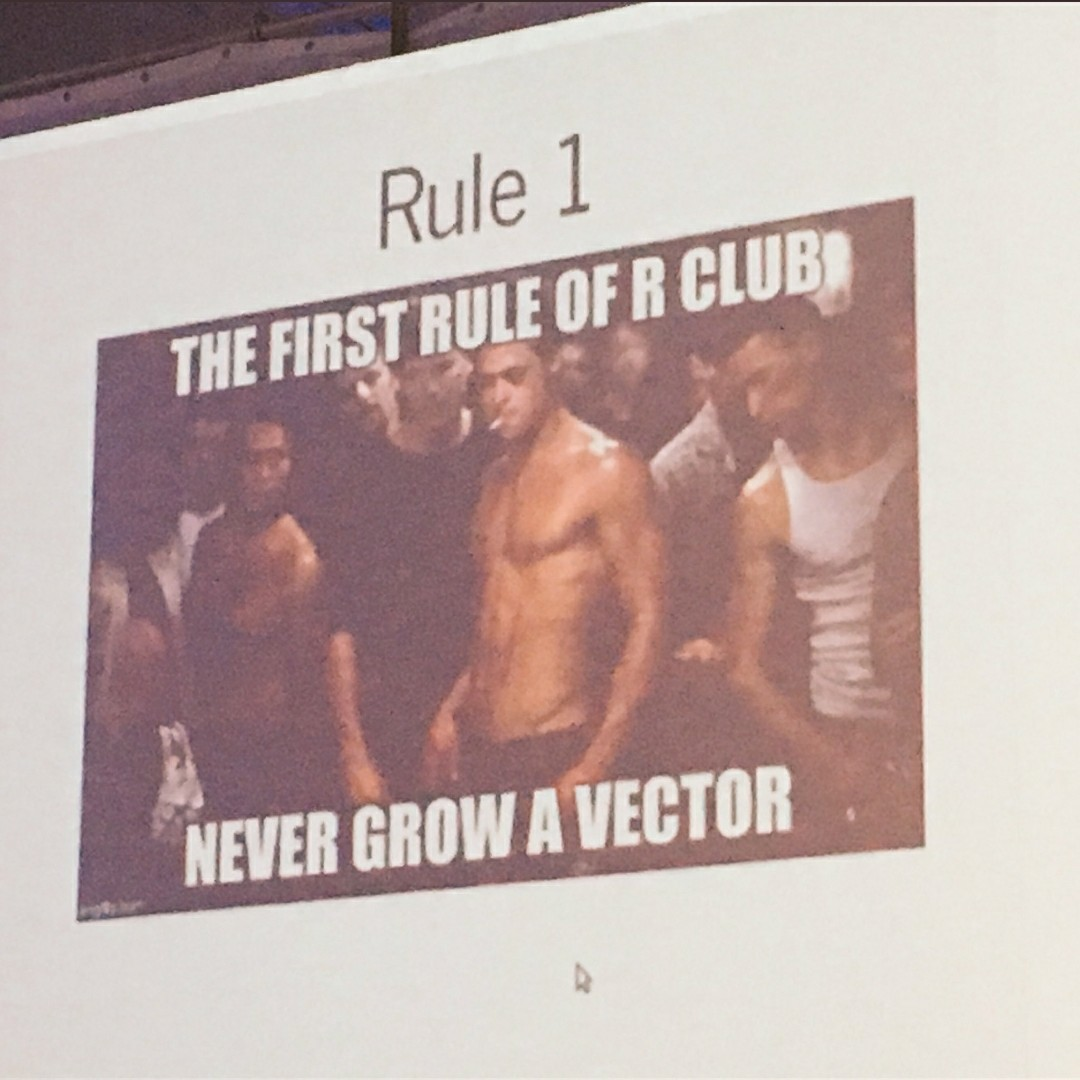
\includegraphics[width=0.9\linewidth]{img/R_club} \end{center}

Voltando ao exemplo das notas, por exemplo, o cálculo da média simples
poderia ser feito diretamente com a função \texttt{apply()}

\begin{Shaded}
\begin{Highlighting}[]
\NormalTok{notas}\SpecialCharTok{$}\NormalTok{media.apply }\OtherTok{\textless{}{-}} \FunctionTok{apply}\NormalTok{(}\AttributeTok{X =}\NormalTok{ notas[, provas], }\AttributeTok{MARGIN =} \DecValTok{1}\NormalTok{, }\AttributeTok{FUN =}\NormalTok{ mean)}
\FunctionTok{head}\NormalTok{(notas)}
\NormalTok{     nome prova1 prova2 prova3    media   media2   media3        CV  MP}
\DecValTok{1}\NormalTok{ Aluno\_1      }\DecValTok{8}      \DecValTok{4}      \DecValTok{1} \FloatTok{4.333333} \FloatTok{4.333333} \FloatTok{4.333333} \FloatTok{0.8104349} \FloatTok{4.0}
\DecValTok{2}\NormalTok{ Aluno\_2      }\DecValTok{2}      \DecValTok{7}      \DecValTok{6} \FloatTok{5.000000} \FloatTok{5.000000} \FloatTok{5.000000} \FloatTok{0.5291503} \FloatTok{5.1}
\DecValTok{3}\NormalTok{ Aluno\_3      }\DecValTok{9}      \DecValTok{2}      \DecValTok{4} \FloatTok{5.000000} \FloatTok{5.000000} \FloatTok{5.000000} \FloatTok{0.7211103} \FloatTok{4.9}
\DecValTok{4}\NormalTok{ Aluno\_4      }\DecValTok{1}     \DecValTok{10}      \DecValTok{9} \FloatTok{6.666667} \FloatTok{6.666667} \FloatTok{6.666667} \FloatTok{0.7399324} \FloatTok{6.9}
\DecValTok{5}\NormalTok{ Aluno\_5      }\DecValTok{7}      \DecValTok{6}      \DecValTok{8} \FloatTok{7.000000} \FloatTok{7.000000} \FloatTok{7.000000} \FloatTok{0.1428571} \FloatTok{7.1}
\DecValTok{6}\NormalTok{ Aluno\_6     }\DecValTok{10}      \DecValTok{0}      \DecValTok{3} \FloatTok{4.333333} \FloatTok{4.333333} \FloatTok{4.333333} \FloatTok{1.1842157} \FloatTok{4.2}
\NormalTok{       MP2  situacao media.apply}
\DecValTok{1} \FloatTok{4.333333}\NormalTok{ reprovado    }\FloatTok{4.333333}
\DecValTok{2} \FloatTok{5.000000}\NormalTok{ reprovado    }\FloatTok{5.000000}
\DecValTok{3} \FloatTok{5.000000}\NormalTok{ reprovado    }\FloatTok{5.000000}
\DecValTok{4} \FloatTok{6.666667}\NormalTok{ reprovado    }\FloatTok{6.666667}
\DecValTok{5} \FloatTok{7.000000}\NormalTok{  aprovado    }\FloatTok{7.000000}
\DecValTok{6} \FloatTok{4.333333}\NormalTok{ reprovado    }\FloatTok{4.333333}
\end{Highlighting}
\end{Shaded}

As médias ponderadas poderiam ser calculadas da mesma forma, e usando a
função que criamos anteriormente

\begin{Shaded}
\begin{Highlighting}[]
\NormalTok{notas}\SpecialCharTok{$}\NormalTok{MP.apply }\OtherTok{\textless{}{-}} \FunctionTok{apply}\NormalTok{(}\AttributeTok{X =}\NormalTok{ notas[, provas], }\AttributeTok{MARGIN =} \DecValTok{1}\NormalTok{, }\AttributeTok{FUN =}\NormalTok{ med.pond)}
\FunctionTok{head}\NormalTok{(notas)}
\NormalTok{     nome prova1 prova2 prova3    media   media2   media3        CV  MP}
\DecValTok{1}\NormalTok{ Aluno\_1      }\DecValTok{8}      \DecValTok{4}      \DecValTok{1} \FloatTok{4.333333} \FloatTok{4.333333} \FloatTok{4.333333} \FloatTok{0.8104349} \FloatTok{4.0}
\DecValTok{2}\NormalTok{ Aluno\_2      }\DecValTok{2}      \DecValTok{7}      \DecValTok{6} \FloatTok{5.000000} \FloatTok{5.000000} \FloatTok{5.000000} \FloatTok{0.5291503} \FloatTok{5.1}
\DecValTok{3}\NormalTok{ Aluno\_3      }\DecValTok{9}      \DecValTok{2}      \DecValTok{4} \FloatTok{5.000000} \FloatTok{5.000000} \FloatTok{5.000000} \FloatTok{0.7211103} \FloatTok{4.9}
\DecValTok{4}\NormalTok{ Aluno\_4      }\DecValTok{1}     \DecValTok{10}      \DecValTok{9} \FloatTok{6.666667} \FloatTok{6.666667} \FloatTok{6.666667} \FloatTok{0.7399324} \FloatTok{6.9}
\DecValTok{5}\NormalTok{ Aluno\_5      }\DecValTok{7}      \DecValTok{6}      \DecValTok{8} \FloatTok{7.000000} \FloatTok{7.000000} \FloatTok{7.000000} \FloatTok{0.1428571} \FloatTok{7.1}
\DecValTok{6}\NormalTok{ Aluno\_6     }\DecValTok{10}      \DecValTok{0}      \DecValTok{3} \FloatTok{4.333333} \FloatTok{4.333333} \FloatTok{4.333333} \FloatTok{1.1842157} \FloatTok{4.2}
\NormalTok{       MP2  situacao media.apply MP.apply}
\DecValTok{1} \FloatTok{4.333333}\NormalTok{ reprovado    }\FloatTok{4.333333} \FloatTok{4.333333}
\DecValTok{2} \FloatTok{5.000000}\NormalTok{ reprovado    }\FloatTok{5.000000} \FloatTok{5.000000}
\DecValTok{3} \FloatTok{5.000000}\NormalTok{ reprovado    }\FloatTok{5.000000} \FloatTok{5.000000}
\DecValTok{4} \FloatTok{6.666667}\NormalTok{ reprovado    }\FloatTok{6.666667} \FloatTok{6.666667}
\DecValTok{5} \FloatTok{7.000000}\NormalTok{  aprovado    }\FloatTok{7.000000} \FloatTok{7.000000}
\DecValTok{6} \FloatTok{4.333333}\NormalTok{ reprovado    }\FloatTok{4.333333} \FloatTok{4.333333}
\end{Highlighting}
\end{Shaded}

Mas note que como temos o argumento \texttt{pesos} especificado com um padrão,
devemos alterar na própria função \texttt{apply()}

\begin{Shaded}
\begin{Highlighting}[]
\NormalTok{notas}\SpecialCharTok{$}\NormalTok{MP.apply }\OtherTok{\textless{}{-}} \FunctionTok{apply}\NormalTok{(}\AttributeTok{X =}\NormalTok{ notas[, provas], }\AttributeTok{MARGIN =} \DecValTok{1}\NormalTok{,}
                        \AttributeTok{FUN =}\NormalTok{ med.pond, }\AttributeTok{pesos =} \FunctionTok{c}\NormalTok{(}\DecValTok{3}\NormalTok{, }\DecValTok{3}\NormalTok{, }\DecValTok{4}\NormalTok{))}
\FunctionTok{head}\NormalTok{(notas)}
\NormalTok{     nome prova1 prova2 prova3    media   media2   media3        CV  MP}
\DecValTok{1}\NormalTok{ Aluno\_1      }\DecValTok{8}      \DecValTok{4}      \DecValTok{1} \FloatTok{4.333333} \FloatTok{4.333333} \FloatTok{4.333333} \FloatTok{0.8104349} \FloatTok{4.0}
\DecValTok{2}\NormalTok{ Aluno\_2      }\DecValTok{2}      \DecValTok{7}      \DecValTok{6} \FloatTok{5.000000} \FloatTok{5.000000} \FloatTok{5.000000} \FloatTok{0.5291503} \FloatTok{5.1}
\DecValTok{3}\NormalTok{ Aluno\_3      }\DecValTok{9}      \DecValTok{2}      \DecValTok{4} \FloatTok{5.000000} \FloatTok{5.000000} \FloatTok{5.000000} \FloatTok{0.7211103} \FloatTok{4.9}
\DecValTok{4}\NormalTok{ Aluno\_4      }\DecValTok{1}     \DecValTok{10}      \DecValTok{9} \FloatTok{6.666667} \FloatTok{6.666667} \FloatTok{6.666667} \FloatTok{0.7399324} \FloatTok{6.9}
\DecValTok{5}\NormalTok{ Aluno\_5      }\DecValTok{7}      \DecValTok{6}      \DecValTok{8} \FloatTok{7.000000} \FloatTok{7.000000} \FloatTok{7.000000} \FloatTok{0.1428571} \FloatTok{7.1}
\DecValTok{6}\NormalTok{ Aluno\_6     }\DecValTok{10}      \DecValTok{0}      \DecValTok{3} \FloatTok{4.333333} \FloatTok{4.333333} \FloatTok{4.333333} \FloatTok{1.1842157} \FloatTok{4.2}
\NormalTok{       MP2  situacao media.apply MP.apply}
\DecValTok{1} \FloatTok{4.333333}\NormalTok{ reprovado    }\FloatTok{4.333333}      \FloatTok{4.0}
\DecValTok{2} \FloatTok{5.000000}\NormalTok{ reprovado    }\FloatTok{5.000000}      \FloatTok{5.1}
\DecValTok{3} \FloatTok{5.000000}\NormalTok{ reprovado    }\FloatTok{5.000000}      \FloatTok{4.9}
\DecValTok{4} \FloatTok{6.666667}\NormalTok{ reprovado    }\FloatTok{6.666667}      \FloatTok{6.9}
\DecValTok{5} \FloatTok{7.000000}\NormalTok{  aprovado    }\FloatTok{7.000000}      \FloatTok{7.1}
\DecValTok{6} \FloatTok{4.333333}\NormalTok{ reprovado    }\FloatTok{4.333333}      \FloatTok{4.2}
\end{Highlighting}
\end{Shaded}

NOTA: veja que isso é possível devido à presença do argumento \texttt{...} na
função \texttt{apply()}, que permite passar argumentos de outras funções
dentro dela.

Também poderíamos usar a função \texttt{weighted.mean()} implementada no R

\begin{Shaded}
\begin{Highlighting}[]
\NormalTok{notas}\SpecialCharTok{$}\NormalTok{MP2.apply }\OtherTok{\textless{}{-}} \FunctionTok{apply}\NormalTok{(}\AttributeTok{X =}\NormalTok{ notas[, provas], }\AttributeTok{MARGIN =} \DecValTok{1}\NormalTok{,}
                         \AttributeTok{FUN =}\NormalTok{ weighted.mean, }\AttributeTok{w =} \FunctionTok{c}\NormalTok{(}\DecValTok{3}\NormalTok{, }\DecValTok{3}\NormalTok{, }\DecValTok{4}\NormalTok{))}
\FunctionTok{head}\NormalTok{(notas)}
\NormalTok{     nome prova1 prova2 prova3    media   media2   media3        CV  MP}
\DecValTok{1}\NormalTok{ Aluno\_1      }\DecValTok{8}      \DecValTok{4}      \DecValTok{1} \FloatTok{4.333333} \FloatTok{4.333333} \FloatTok{4.333333} \FloatTok{0.8104349} \FloatTok{4.0}
\DecValTok{2}\NormalTok{ Aluno\_2      }\DecValTok{2}      \DecValTok{7}      \DecValTok{6} \FloatTok{5.000000} \FloatTok{5.000000} \FloatTok{5.000000} \FloatTok{0.5291503} \FloatTok{5.1}
\DecValTok{3}\NormalTok{ Aluno\_3      }\DecValTok{9}      \DecValTok{2}      \DecValTok{4} \FloatTok{5.000000} \FloatTok{5.000000} \FloatTok{5.000000} \FloatTok{0.7211103} \FloatTok{4.9}
\DecValTok{4}\NormalTok{ Aluno\_4      }\DecValTok{1}     \DecValTok{10}      \DecValTok{9} \FloatTok{6.666667} \FloatTok{6.666667} \FloatTok{6.666667} \FloatTok{0.7399324} \FloatTok{6.9}
\DecValTok{5}\NormalTok{ Aluno\_5      }\DecValTok{7}      \DecValTok{6}      \DecValTok{8} \FloatTok{7.000000} \FloatTok{7.000000} \FloatTok{7.000000} \FloatTok{0.1428571} \FloatTok{7.1}
\DecValTok{6}\NormalTok{ Aluno\_6     }\DecValTok{10}      \DecValTok{0}      \DecValTok{3} \FloatTok{4.333333} \FloatTok{4.333333} \FloatTok{4.333333} \FloatTok{1.1842157} \FloatTok{4.2}
\NormalTok{       MP2  situacao media.apply MP.apply MP2.apply}
\DecValTok{1} \FloatTok{4.333333}\NormalTok{ reprovado    }\FloatTok{4.333333}      \FloatTok{4.0}       \FloatTok{4.0}
\DecValTok{2} \FloatTok{5.000000}\NormalTok{ reprovado    }\FloatTok{5.000000}      \FloatTok{5.1}       \FloatTok{5.1}
\DecValTok{3} \FloatTok{5.000000}\NormalTok{ reprovado    }\FloatTok{5.000000}      \FloatTok{4.9}       \FloatTok{4.9}
\DecValTok{4} \FloatTok{6.666667}\NormalTok{ reprovado    }\FloatTok{6.666667}      \FloatTok{6.9}       \FloatTok{6.9}
\DecValTok{5} \FloatTok{7.000000}\NormalTok{  aprovado    }\FloatTok{7.000000}      \FloatTok{7.1}       \FloatTok{7.1}
\DecValTok{6} \FloatTok{4.333333}\NormalTok{ reprovado    }\FloatTok{4.333333}      \FloatTok{4.2}       \FloatTok{4.2}
\end{Highlighting}
\end{Shaded}

O Coeficiente de Variação poderia ser calculado usando nossa função
\texttt{cv()}

\begin{Shaded}
\begin{Highlighting}[]
\NormalTok{notas}\SpecialCharTok{$}\NormalTok{CV.apply }\OtherTok{\textless{}{-}} \FunctionTok{apply}\NormalTok{(}\AttributeTok{X =}\NormalTok{ notas[, provas], }\AttributeTok{MARGIN =} \DecValTok{1}\NormalTok{, }\AttributeTok{FUN =}\NormalTok{ cv)}
\FunctionTok{head}\NormalTok{(notas)}
\NormalTok{     nome prova1 prova2 prova3    media   media2   media3        CV  MP}
\DecValTok{1}\NormalTok{ Aluno\_1      }\DecValTok{8}      \DecValTok{4}      \DecValTok{1} \FloatTok{4.333333} \FloatTok{4.333333} \FloatTok{4.333333} \FloatTok{0.8104349} \FloatTok{4.0}
\DecValTok{2}\NormalTok{ Aluno\_2      }\DecValTok{2}      \DecValTok{7}      \DecValTok{6} \FloatTok{5.000000} \FloatTok{5.000000} \FloatTok{5.000000} \FloatTok{0.5291503} \FloatTok{5.1}
\DecValTok{3}\NormalTok{ Aluno\_3      }\DecValTok{9}      \DecValTok{2}      \DecValTok{4} \FloatTok{5.000000} \FloatTok{5.000000} \FloatTok{5.000000} \FloatTok{0.7211103} \FloatTok{4.9}
\DecValTok{4}\NormalTok{ Aluno\_4      }\DecValTok{1}     \DecValTok{10}      \DecValTok{9} \FloatTok{6.666667} \FloatTok{6.666667} \FloatTok{6.666667} \FloatTok{0.7399324} \FloatTok{6.9}
\DecValTok{5}\NormalTok{ Aluno\_5      }\DecValTok{7}      \DecValTok{6}      \DecValTok{8} \FloatTok{7.000000} \FloatTok{7.000000} \FloatTok{7.000000} \FloatTok{0.1428571} \FloatTok{7.1}
\DecValTok{6}\NormalTok{ Aluno\_6     }\DecValTok{10}      \DecValTok{0}      \DecValTok{3} \FloatTok{4.333333} \FloatTok{4.333333} \FloatTok{4.333333} \FloatTok{1.1842157} \FloatTok{4.2}
\NormalTok{       MP2  situacao media.apply MP.apply MP2.apply  CV.apply}
\DecValTok{1} \FloatTok{4.333333}\NormalTok{ reprovado    }\FloatTok{4.333333}      \FloatTok{4.0}       \FloatTok{4.0} \FloatTok{0.8104349}
\DecValTok{2} \FloatTok{5.000000}\NormalTok{ reprovado    }\FloatTok{5.000000}      \FloatTok{5.1}       \FloatTok{5.1} \FloatTok{0.5291503}
\DecValTok{3} \FloatTok{5.000000}\NormalTok{ reprovado    }\FloatTok{5.000000}      \FloatTok{4.9}       \FloatTok{4.9} \FloatTok{0.7211103}
\DecValTok{4} \FloatTok{6.666667}\NormalTok{ reprovado    }\FloatTok{6.666667}      \FloatTok{6.9}       \FloatTok{6.9} \FloatTok{0.7399324}
\DecValTok{5} \FloatTok{7.000000}\NormalTok{  aprovado    }\FloatTok{7.000000}      \FloatTok{7.1}       \FloatTok{7.1} \FloatTok{0.1428571}
\DecValTok{6} \FloatTok{4.333333}\NormalTok{ reprovado    }\FloatTok{4.333333}      \FloatTok{4.2}       \FloatTok{4.2} \FloatTok{1.1842157}
\end{Highlighting}
\end{Shaded}

Finalmente, a estrutura de repetição \texttt{if()} também possui uma forma
vetorizada através da função \texttt{ifelse()}. Essa função funciona da
seguinte forma:

\begin{Shaded}
\begin{Highlighting}[]
\FunctionTok{ifelse}\NormalTok{(}\SpecialCharTok{\textless{}}\NormalTok{condição}\SpecialCharTok{\textgreater{}}\NormalTok{, }\SpecialCharTok{\textless{}}\NormalTok{valor se verdadeiro}\SpecialCharTok{\textgreater{}}\NormalTok{, }\SpecialCharTok{\textless{}}\NormalTok{valor se falso}\SpecialCharTok{\textgreater{}}\NormalTok{)}
\end{Highlighting}
\end{Shaded}

Dessa forma, a atribuição da situação dos alunos poderia ser feita da
seguinte forma:

\begin{Shaded}
\begin{Highlighting}[]
\NormalTok{notas}\SpecialCharTok{$}\NormalTok{situacao2 }\OtherTok{\textless{}{-}} \FunctionTok{ifelse}\NormalTok{(notas}\SpecialCharTok{$}\NormalTok{MP }\SpecialCharTok{\textgreater{}=} \DecValTok{7}\NormalTok{, }\StringTok{"aprovado"}\NormalTok{, }\StringTok{"reprovado"}\NormalTok{)}
\FunctionTok{head}\NormalTok{(notas)}
\NormalTok{     nome prova1 prova2 prova3    media   media2   media3        CV  MP}
\DecValTok{1}\NormalTok{ Aluno\_1      }\DecValTok{8}      \DecValTok{4}      \DecValTok{1} \FloatTok{4.333333} \FloatTok{4.333333} \FloatTok{4.333333} \FloatTok{0.8104349} \FloatTok{4.0}
\DecValTok{2}\NormalTok{ Aluno\_2      }\DecValTok{2}      \DecValTok{7}      \DecValTok{6} \FloatTok{5.000000} \FloatTok{5.000000} \FloatTok{5.000000} \FloatTok{0.5291503} \FloatTok{5.1}
\DecValTok{3}\NormalTok{ Aluno\_3      }\DecValTok{9}      \DecValTok{2}      \DecValTok{4} \FloatTok{5.000000} \FloatTok{5.000000} \FloatTok{5.000000} \FloatTok{0.7211103} \FloatTok{4.9}
\DecValTok{4}\NormalTok{ Aluno\_4      }\DecValTok{1}     \DecValTok{10}      \DecValTok{9} \FloatTok{6.666667} \FloatTok{6.666667} \FloatTok{6.666667} \FloatTok{0.7399324} \FloatTok{6.9}
\DecValTok{5}\NormalTok{ Aluno\_5      }\DecValTok{7}      \DecValTok{6}      \DecValTok{8} \FloatTok{7.000000} \FloatTok{7.000000} \FloatTok{7.000000} \FloatTok{0.1428571} \FloatTok{7.1}
\DecValTok{6}\NormalTok{ Aluno\_6     }\DecValTok{10}      \DecValTok{0}      \DecValTok{3} \FloatTok{4.333333} \FloatTok{4.333333} \FloatTok{4.333333} \FloatTok{1.1842157} \FloatTok{4.2}
\NormalTok{       MP2  situacao media.apply MP.apply MP2.apply  CV.apply situacao2}
\DecValTok{1} \FloatTok{4.333333}\NormalTok{ reprovado    }\FloatTok{4.333333}      \FloatTok{4.0}       \FloatTok{4.0} \FloatTok{0.8104349}\NormalTok{ reprovado}
\DecValTok{2} \FloatTok{5.000000}\NormalTok{ reprovado    }\FloatTok{5.000000}      \FloatTok{5.1}       \FloatTok{5.1} \FloatTok{0.5291503}\NormalTok{ reprovado}
\DecValTok{3} \FloatTok{5.000000}\NormalTok{ reprovado    }\FloatTok{5.000000}      \FloatTok{4.9}       \FloatTok{4.9} \FloatTok{0.7211103}\NormalTok{ reprovado}
\DecValTok{4} \FloatTok{6.666667}\NormalTok{ reprovado    }\FloatTok{6.666667}      \FloatTok{6.9}       \FloatTok{6.9} \FloatTok{0.7399324}\NormalTok{ reprovado}
\DecValTok{5} \FloatTok{7.000000}\NormalTok{  aprovado    }\FloatTok{7.000000}      \FloatTok{7.1}       \FloatTok{7.1} \FloatTok{0.1428571}\NormalTok{  aprovado}
\DecValTok{6} \FloatTok{4.333333}\NormalTok{ reprovado    }\FloatTok{4.333333}      \FloatTok{4.2}       \FloatTok{4.2} \FloatTok{1.1842157}\NormalTok{ reprovado}
\end{Highlighting}
\end{Shaded}

\hypertarget{exercuxedcios-13}{%
\subsection*{Exercícios}\label{exercuxedcios-13}}


\begin{enumerate}
\def\labelenumi{\arabic{enumi}.}
\tightlist
\item
  Faça uma função usando loop for que recebe duas matrizes de mesma dimensão e retorna a soma das matrizes. Note que é necessário verificar se as matrizes fornecidas pelo usuário podem ser somadas, caso contrário retorne uma mensagem de erro dizendo que as matrizes não podem ser somadas.
\item
  Faça uma função usando loop for para multiplicar duas matrizes compatíveis. Note que é necessário verificar se as matrizes fornecidas pelo usuário podem ser multiplicadas, caso contrário retorne uma mensagem de erro dizendo que as matrizes não podem ser multiplicadas.
\item
  Faça uma função para resolver sistemas lineares 2 x 2 usando o método de decomposição de Gauss. Veja esta página se você não conhece o método \url{https://matrixcalc.org/pt/slu.html}.
\item
  Faça uma função que encontra o máximo de uma função fornecida pelo usuário em um intervalo e precisão pré-determinado pelo usuário.
\item
  Faça uma função que resolve uma equação não-linear de um único parâmetro em um intervalo e precisão pré-determinado pelo usuário.
\end{enumerate}

\hypertarget{outras-estruturas-while-e-repeat}{%
\section{Outras estruturas: while e repeat}\label{outras-estruturas-while-e-repeat}}

O \texttt{while} executa comandos enquanto uma determinada condição permanece
verdadeira.

\begin{Shaded}
\begin{Highlighting}[]
\DocumentationTok{\#\# Calcule a soma em 1,2,3... até que o soma seja maior do que 1000}
\NormalTok{n }\OtherTok{\textless{}{-}} \DecValTok{0}
\NormalTok{soma }\OtherTok{\textless{}{-}} \DecValTok{0}
\ControlFlowTok{while}\NormalTok{(soma }\SpecialCharTok{\textless{}=} \DecValTok{1000}\NormalTok{)\{}
\NormalTok{    n }\OtherTok{\textless{}{-}}\NormalTok{ n }\SpecialCharTok{+} \DecValTok{1}
\NormalTok{    soma }\OtherTok{\textless{}{-}}\NormalTok{ soma }\SpecialCharTok{+}\NormalTok{ n}
\NormalTok{\}}
\NormalTok{soma}
\NormalTok{[}\DecValTok{1}\NormalTok{] }\DecValTok{1035}
\end{Highlighting}
\end{Shaded}

O \texttt{repeat} é ainda mais básico, e irá executar comandos até que você
explicitamente pare a execução com o comando \texttt{break}.

\begin{Shaded}
\begin{Highlighting}[]
\DocumentationTok{\#\# Mesmo exemplo}
\NormalTok{n }\OtherTok{\textless{}{-}} \DecValTok{0}
\NormalTok{soma }\OtherTok{\textless{}{-}} \DecValTok{0}
\ControlFlowTok{repeat}\NormalTok{\{}
\NormalTok{    n }\OtherTok{\textless{}{-}}\NormalTok{ n }\SpecialCharTok{+} \DecValTok{1}
\NormalTok{    soma }\OtherTok{\textless{}{-}}\NormalTok{ soma }\SpecialCharTok{+}\NormalTok{ n}
    \ControlFlowTok{if}\NormalTok{(soma }\SpecialCharTok{\textgreater{}} \DecValTok{1000}\NormalTok{) }\ControlFlowTok{break}
\NormalTok{\}}
\NormalTok{soma}
\NormalTok{[}\DecValTok{1}\NormalTok{] }\DecValTok{1035}
\end{Highlighting}
\end{Shaded}

\hypertarget{exercuxedcios-14}{%
\subsection*{Exercícios}\label{exercuxedcios-14}}


\begin{enumerate}
\def\labelenumi{\arabic{enumi}.}
\tightlist
\item
  Crie uma função que retorna o absoluto de um vetor de inteiros.
\item
  Crie uma função em R que retorna o maior valor em um vetor de elementos númericos.
\item
  Crie uma função que retorna o número de valores maiores que a média de um vetor. Você pode usar a função mean().
\item
  Crie uma função que dado um vetor de tamanho 3 retorna os seus valores em ordem crescente e decrescente.
\item
  Crie uma função que calcula o fatorial de um número.
\end{enumerate}

\hypertarget{part-estatuxedstica}{%
\part{Estatística}\label{part-estatuxedstica}}

\hypertarget{anuxe1lise-exploratuxf3ria-de-dados}{%
\chapter{Análise exploratória de dados}\label{anuxe1lise-exploratuxf3ria-de-dados}}

Nesta sessão vamos ver alguns (mas não todos!) comandos do R para fazer
uma análise descritiva de um conjunto de dados.

Uma boa forma de iniciar uma análise descritiva adequada é verificar os
tipos de variáveis disponíveis. Variáveis podem ser classificadas da
seguinte forma:

\begin{itemize}
\tightlist
\item
  Qualitativas

  \begin{itemize}
  \tightlist
  \item
    Nominais
  \item
    Ordinais
  \end{itemize}
\item
  Quantitativas

  \begin{itemize}
  \tightlist
  \item
    Discretas
  \item
    Contínuas
  \end{itemize}
\end{itemize}

e podem ser resumidas por tabelas, gráficos e/ou medidas de tendência central e dispersão.

\hypertarget{o-conjunto-de-dados-milsa}{%
\section{\texorpdfstring{O conjunto de dados \texttt{milsa}}{O conjunto de dados milsa}}\label{o-conjunto-de-dados-milsa}}

O livro ``Estatística Básica'' de W. O. Bussab e P. A. Morettin traz no
segundo capítulo um conjunto de dados hipotético de atributos de 36
funcionários da companhia ``Milsa''. Os dados estão reproduzidos na tabela
abaixo. Consulte o livro para mais detalhes sobre este dados.

\begin{tabular}{r|l|l|r|r|r|r|l}
\hline
Funcionario & Est.civil & Inst & Filhos & Salario & Anos & Meses & Regiao\\
\hline
1 & solteiro & 1o Grau & NA & 4.00 & 26 & 3 & interior\\
\hline
2 & casado & 1o Grau & 1 & 4.56 & 32 & 10 & capital\\
\hline
3 & casado & 1o Grau & 2 & 5.25 & 36 & 5 & capital\\
\hline
4 & solteiro & 2o Grau & NA & 5.73 & 20 & 10 & outro\\
\hline
5 & solteiro & 1o Grau & NA & 6.26 & 40 & 7 & outro\\
\hline
6 & casado & 1o Grau & 0 & 6.66 & 28 & 0 & interior\\
\hline
7 & solteiro & 1o Grau & NA & 6.86 & 41 & 0 & interior\\
\hline
8 & solteiro & 1o Grau & NA & 7.39 & 43 & 4 & capital\\
\hline
9 & casado & 2o Grau & 1 & 7.59 & 34 & 10 & capital\\
\hline
10 & solteiro & 2o Grau & NA & 7.44 & 23 & 6 & outro\\
\hline
11 & casado & 2o Grau & 2 & 8.12 & 33 & 6 & interior\\
\hline
12 & solteiro & 1o Grau & NA & 8.46 & 27 & 11 & capital\\
\hline
13 & solteiro & 2o Grau & NA & 8.74 & 37 & 5 & outro\\
\hline
14 & casado & 1o Grau & 3 & 8.95 & 44 & 2 & outro\\
\hline
15 & casado & 2o Grau & 0 & 9.13 & 30 & 5 & interior\\
\hline
16 & solteiro & 2o Grau & NA & 9.35 & 38 & 8 & outro\\
\hline
17 & casado & 2o Grau & 1 & 9.77 & 31 & 7 & capital\\
\hline
18 & casado & 1o Grau & 2 & 9.80 & 39 & 7 & outro\\
\hline
19 & solteiro & Superior & NA & 10.53 & 25 & 8 & interior\\
\hline
20 & solteiro & 2o Grau & NA & 10.76 & 37 & 4 & interior\\
\hline
21 & casado & 2o Grau & 1 & 11.06 & 30 & 9 & outro\\
\hline
22 & solteiro & 2o Grau & NA & 11.59 & 34 & 2 & capital\\
\hline
23 & solteiro & 1o Grau & NA & 12.00 & 41 & 0 & outro\\
\hline
24 & casado & Superior & 0 & 12.79 & 26 & 1 & outro\\
\hline
25 & casado & 2o Grau & 2 & 13.23 & 32 & 5 & interior\\
\hline
26 & casado & 2o Grau & 2 & 13.60 & 35 & 0 & outro\\
\hline
27 & solteiro & 1o Grau & NA & 13.85 & 46 & 7 & outro\\
\hline
28 & casado & 2o Grau & 0 & 14.69 & 29 & 8 & interior\\
\hline
29 & casado & 2o Grau & 5 & 14.71 & 40 & 6 & interior\\
\hline
30 & casado & 2o Grau & 2 & 15.99 & 35 & 10 & capital\\
\hline
31 & solteiro & Superior & NA & 16.22 & 31 & 5 & outro\\
\hline
32 & casado & 2o Grau & 1 & 16.61 & 36 & 4 & interior\\
\hline
33 & casado & Superior & 3 & 17.26 & 43 & 7 & capital\\
\hline
34 & solteiro & Superior & NA & 18.75 & 33 & 7 & capital\\
\hline
35 & casado & 2o Grau & 2 & 19.40 & 48 & 11 & capital\\
\hline
36 & casado & Superior & 3 & 23.30 & 42 & 2 & interior\\
\hline
\end{tabular}

Estes dados estão disponíveis em um arquivo \texttt{csv} no endereço
\url{http://www.leg.ufpr.br/~fernandomayer/data/milsa.csv}.

O nosso objetivo é, através do R,

\begin{itemize}
\tightlist
\item
  Entrar com os dados;
\item
  Fazer uma análise descritiva.
\end{itemize}

Estes são dados no ``estilo planilha'', com variáveis de diferentes tipos:
categóricas e numéricas (qualitativas e quantitativas). Portanto o
formato ideal de armazenamento destes dados no R é o \texttt{data.frame}.

Para importar os dados do endereço acima diretamente para o R, usamos

\begin{Shaded}
\begin{Highlighting}[]
\NormalTok{url }\OtherTok{\textless{}{-}} \StringTok{"http://www.leg.ufpr.br/\textasciitilde{}fernandomayer/data/milsa.csv"}
\NormalTok{milsa }\OtherTok{\textless{}{-}} \FunctionTok{read.csv}\NormalTok{(url)}
\end{Highlighting}
\end{Shaded}

E para conferir a estrutura dos dados podemos usar algumas funções como:

\begin{Shaded}
\begin{Highlighting}[]
\FunctionTok{str}\NormalTok{(milsa)}
\StringTok{\textquotesingle{}data.frame\textquotesingle{}}\SpecialCharTok{:}   \DecValTok{36}\NormalTok{ obs. of  }\DecValTok{8}\NormalTok{ variables}\SpecialCharTok{:}
 \ErrorTok{$}\NormalTok{ Funcionario}\SpecialCharTok{:}\NormalTok{ int  }\DecValTok{1} \DecValTok{2} \DecValTok{3} \DecValTok{4} \DecValTok{5} \DecValTok{6} \DecValTok{7} \DecValTok{8} \DecValTok{9} \DecValTok{10}\NormalTok{ ...}
 \SpecialCharTok{$}\NormalTok{ Est.civil  }\SpecialCharTok{:}\NormalTok{ chr  }\StringTok{"solteiro"} \StringTok{"casado"} \StringTok{"casado"} \StringTok{"solteiro"}\NormalTok{ ...}
 \SpecialCharTok{$}\NormalTok{ Inst       }\SpecialCharTok{:}\NormalTok{ chr  }\StringTok{"1o Grau"} \StringTok{"1o Grau"} \StringTok{"1o Grau"} \StringTok{"2o Grau"}\NormalTok{ ...}
 \SpecialCharTok{$}\NormalTok{ Filhos     }\SpecialCharTok{:}\NormalTok{ int  }\ConstantTok{NA} \DecValTok{1} \DecValTok{2} \ConstantTok{NA} \ConstantTok{NA} \DecValTok{0} \ConstantTok{NA} \ConstantTok{NA} \DecValTok{1} \ConstantTok{NA}\NormalTok{ ...}
 \SpecialCharTok{$}\NormalTok{ Salario    }\SpecialCharTok{:}\NormalTok{ num  }\DecValTok{4} \FloatTok{4.56} \FloatTok{5.25} \FloatTok{5.73} \FloatTok{6.26} \FloatTok{6.66} \FloatTok{6.86} \FloatTok{7.39} \FloatTok{7.59} \FloatTok{7.44}\NormalTok{ ...}
 \SpecialCharTok{$}\NormalTok{ Anos       }\SpecialCharTok{:}\NormalTok{ int  }\DecValTok{26} \DecValTok{32} \DecValTok{36} \DecValTok{20} \DecValTok{40} \DecValTok{28} \DecValTok{41} \DecValTok{43} \DecValTok{34} \DecValTok{23}\NormalTok{ ...}
 \SpecialCharTok{$}\NormalTok{ Meses      }\SpecialCharTok{:}\NormalTok{ int  }\DecValTok{3} \DecValTok{10} \DecValTok{5} \DecValTok{10} \DecValTok{7} \DecValTok{0} \DecValTok{0} \DecValTok{4} \DecValTok{10} \DecValTok{6}\NormalTok{ ...}
 \SpecialCharTok{$}\NormalTok{ Regiao     }\SpecialCharTok{:}\NormalTok{ chr  }\StringTok{"interior"} \StringTok{"capital"} \StringTok{"capital"} \StringTok{"outro"}\NormalTok{ ...}
\FunctionTok{head}\NormalTok{(milsa)}
\NormalTok{  Funcionario Est.civil    Inst Filhos Salario Anos Meses   Regiao}
\DecValTok{1}           \DecValTok{1}\NormalTok{  solteiro 1o Grau     }\ConstantTok{NA}    \FloatTok{4.00}   \DecValTok{26}     \DecValTok{3}\NormalTok{ interior}
\DecValTok{2}           \DecValTok{2}\NormalTok{    casado 1o Grau      }\DecValTok{1}    \FloatTok{4.56}   \DecValTok{32}    \DecValTok{10}\NormalTok{  capital}
\DecValTok{3}           \DecValTok{3}\NormalTok{    casado 1o Grau      }\DecValTok{2}    \FloatTok{5.25}   \DecValTok{36}     \DecValTok{5}\NormalTok{  capital}
\DecValTok{4}           \DecValTok{4}\NormalTok{  solteiro 2o Grau     }\ConstantTok{NA}    \FloatTok{5.73}   \DecValTok{20}    \DecValTok{10}\NormalTok{    outro}
\DecValTok{5}           \DecValTok{5}\NormalTok{  solteiro 1o Grau     }\ConstantTok{NA}    \FloatTok{6.26}   \DecValTok{40}     \DecValTok{7}\NormalTok{    outro}
\DecValTok{6}           \DecValTok{6}\NormalTok{    casado 1o Grau      }\DecValTok{0}    \FloatTok{6.66}   \DecValTok{28}     \DecValTok{0}\NormalTok{ interior}
\FunctionTok{tail}\NormalTok{(milsa)}
\NormalTok{   Funcionario Est.civil     Inst Filhos Salario Anos Meses   Regiao}
\DecValTok{31}          \DecValTok{31}\NormalTok{  solteiro Superior     }\ConstantTok{NA}   \FloatTok{16.22}   \DecValTok{31}     \DecValTok{5}\NormalTok{    outro}
\DecValTok{32}          \DecValTok{32}\NormalTok{    casado  2o Grau      }\DecValTok{1}   \FloatTok{16.61}   \DecValTok{36}     \DecValTok{4}\NormalTok{ interior}
\DecValTok{33}          \DecValTok{33}\NormalTok{    casado Superior      }\DecValTok{3}   \FloatTok{17.26}   \DecValTok{43}     \DecValTok{7}\NormalTok{  capital}
\DecValTok{34}          \DecValTok{34}\NormalTok{  solteiro Superior     }\ConstantTok{NA}   \FloatTok{18.75}   \DecValTok{33}     \DecValTok{7}\NormalTok{  capital}
\DecValTok{35}          \DecValTok{35}\NormalTok{    casado  2o Grau      }\DecValTok{2}   \FloatTok{19.40}   \DecValTok{48}    \DecValTok{11}\NormalTok{  capital}
\DecValTok{36}          \DecValTok{36}\NormalTok{    casado Superior      }\DecValTok{3}   \FloatTok{23.30}   \DecValTok{42}     \DecValTok{2}\NormalTok{ interior}
\end{Highlighting}
\end{Shaded}

Podemos classificar todas as variáveis desse conjunto de dados como:

\begin{longtable}[]{@{}ll@{}}
\toprule()
Variável & Classificação \\
\midrule()
\endhead
\texttt{Funcionario} & Quantitativa discreta \\
\texttt{Est.civil} & Qualitativa nominal \\
\texttt{Inst} & Qualitativa ordinal \\
\texttt{Filhos} & Quantitativa discreta \\
\texttt{Salario} & Quantitativa contínua \\
\texttt{Anos} & Quantitativa contínua \\
\texttt{Meses} & Quantitativa contínua \\
\texttt{Regiao} & Qualitativa nominal \\
\bottomrule()
\end{longtable}

Como a variável \texttt{Inst} é qualitativa ordinal, podemos indicar para o R
que ela deve ser tratada como ordinal. Se observarmos os níveis desse
fator:

\begin{Shaded}
\begin{Highlighting}[]
\FunctionTok{levels}\NormalTok{(milsa}\SpecialCharTok{$}\NormalTok{Inst)}
\ConstantTok{NULL}
\end{Highlighting}
\end{Shaded}

já notamos que a ordenação está correta (da esquerda para a direita),
pois sabemos que a classificação interna dos níveis é por ordem
alfabética, e nesse caso, por coincidência, a ordem já está na sequência
correta. Mesmo assim, podemos indicar que este fator é ordinal, usando o
argumento \texttt{ordered} da função \texttt{factor()}

\begin{Shaded}
\begin{Highlighting}[]
\NormalTok{milsa}\SpecialCharTok{$}\NormalTok{Inst }\OtherTok{\textless{}{-}} \FunctionTok{factor}\NormalTok{(milsa}\SpecialCharTok{$}\NormalTok{Inst, }\AttributeTok{ordered =} \ConstantTok{TRUE}\NormalTok{)}
\end{Highlighting}
\end{Shaded}

Note agora a modificação na classe dessa coluna, e a representação dos
níveis:

\begin{Shaded}
\begin{Highlighting}[]
\FunctionTok{class}\NormalTok{(milsa}\SpecialCharTok{$}\NormalTok{Inst)}
\NormalTok{[}\DecValTok{1}\NormalTok{] }\StringTok{"ordered"} \StringTok{"factor"} 
\NormalTok{milsa}\SpecialCharTok{$}\NormalTok{Inst}
\NormalTok{ [}\DecValTok{1}\NormalTok{] 1o Grau  1o Grau  1o Grau  2o Grau  1o Grau  1o Grau  1o Grau  1o Grau }
\NormalTok{ [}\DecValTok{9}\NormalTok{] 2o Grau  2o Grau  2o Grau  1o Grau  2o Grau  1o Grau  2o Grau  2o Grau }
\NormalTok{[}\DecValTok{17}\NormalTok{] 2o Grau  1o Grau  Superior 2o Grau  2o Grau  2o Grau  1o Grau  Superior}
\NormalTok{[}\DecValTok{25}\NormalTok{] 2o Grau  2o Grau  1o Grau  2o Grau  2o Grau  2o Grau  Superior 2o Grau }
\NormalTok{[}\DecValTok{33}\NormalTok{] Superior Superior 2o Grau  Superior}
\NormalTok{Levels}\SpecialCharTok{:}\NormalTok{ 1o Grau }\SpecialCharTok{\textless{}}\NormalTok{ 2o Grau }\SpecialCharTok{\textless{}}\NormalTok{ Superior}
\end{Highlighting}
\end{Shaded}

A coluna continua sendo um \texttt{factor}, mas agora também é \texttt{ordered} (sim,
um objeto pode ter mais de uma classe, se elas foram compatíveis e/ou
complementares). Os níveis agora são representados por

\begin{verbatim}
1o Grau < 2o Grau < Superior
\end{verbatim}

para indicar explicitamente que existe uma ordem nos níveis desse fator.

Podemos ainda definir uma nova variável, chamada \texttt{Idade}, a partir das
variáveis \texttt{Anos} e \texttt{Meses}:

\begin{Shaded}
\begin{Highlighting}[]
\NormalTok{milsa}\SpecialCharTok{$}\NormalTok{Idade }\OtherTok{\textless{}{-}}\NormalTok{ milsa}\SpecialCharTok{$}\NormalTok{Anos }\SpecialCharTok{+}\NormalTok{ milsa}\SpecialCharTok{$}\NormalTok{Meses}\SpecialCharTok{/}\DecValTok{12}
\end{Highlighting}
\end{Shaded}

Os dois comandos acima (de modificação da classe de uma variável, e a
criação de uma nova variável) poderiam ser facilmente executadas de uma
única vez através do comando \texttt{transform()}

\begin{Shaded}
\begin{Highlighting}[]
\NormalTok{milsa }\OtherTok{\textless{}{-}} \FunctionTok{transform}\NormalTok{(milsa,}
                   \AttributeTok{Inst =} \FunctionTok{factor}\NormalTok{(Inst, }\AttributeTok{ordered =} \ConstantTok{TRUE}\NormalTok{),}
                   \AttributeTok{Idade =}\NormalTok{ Anos }\SpecialCharTok{+}\NormalTok{ Meses}\SpecialCharTok{/}\DecValTok{12}\NormalTok{)}
\end{Highlighting}
\end{Shaded}

Agora que os dados estão prontos podemos começar a análise descritiva.
A seguir mostramos como fazer análises descritivas uni e bivariadas.
Inspecione os comandos mostrados a seguir e os resultados por eles
produzidos. Sugerimos ainda que o leitor use o R para reproduzir os
resultados mostrados no texto dos capítulos 1 a 3 do livro de Bussab \&
Morettin, relacionados com este exemplo. Veja os scripts do livro
\href{https://rpubs.com/EstatBasica/Introd}{aqui}.

\hypertarget{anuxe1lise-univariada}{%
\section{Análise univariada}\label{anuxe1lise-univariada}}

A análise univariada consiste basicamente em, para cada uma das
variáveis individualmente:

\begin{itemize}
\tightlist
\item
  Classificar a variável quanto a seu tipo: qualitativa (nominal ou
  ordinal) ou quantitativa (discreta ou contínua).
\item
  Obter tabelas, gráficos e/ou medidas que resumam a variável.
\end{itemize}

A partir destes resultados pode-se montar um resumo geral dos dados.

A seguir vamos mostrar como obter tabelas, gráficos e medidas com o R.
Para isto vamos selecionar uma variável de cada tipo para que o leitor
possa, por analogia, obter resultados para as demais.

\hypertarget{variuxe1vel-qualitativa-nominal}{%
\subsection{Variável Qualitativa Nominal}\label{variuxe1vel-qualitativa-nominal}}

A variável \texttt{Est.civil} é uma qualitativa nominal. Desta forma podemos
obter: (i) uma tabela de frequências (absolutas e/ou relativas), (ii) um
gráfico de setores, (iii) a ``moda'', \emph{i.e.} o valor que ocorre com maior
frequência.

Já vimos, através do resultado da função \texttt{str()} acima, que esta
variável é um fator. A seguir obtemos frequências absolutas e relativas
(note duas formas diferentes de obter as frequências relativas).

\begin{Shaded}
\begin{Highlighting}[]
\DocumentationTok{\#\# Frequência absoluta}
\NormalTok{civil.tb }\OtherTok{\textless{}{-}} \FunctionTok{table}\NormalTok{(milsa}\SpecialCharTok{$}\NormalTok{Est.civil)}
\NormalTok{civil.tb}

\NormalTok{  casado solteiro }
      \DecValTok{20}       \DecValTok{16} 
\DocumentationTok{\#\# Frequência relativa, calculando manualmente}
\NormalTok{civil.tb}\SpecialCharTok{/}\FunctionTok{length}\NormalTok{(milsa}\SpecialCharTok{$}\NormalTok{Est.civil)}

\NormalTok{   casado  solteiro }
\FloatTok{0.5555556} \FloatTok{0.4444444} 
\DocumentationTok{\#\# Frequência relativa, com a função prop.table()}
\FunctionTok{prop.table}\NormalTok{(civil.tb)}

\NormalTok{   casado  solteiro }
\FloatTok{0.5555556} \FloatTok{0.4444444} 
\end{Highlighting}
\end{Shaded}

Os gráficos de barras e de setores são adequados para representar esta
variável. Os comandos \texttt{barplot()} e \texttt{pie()} usam o resultado da função
\texttt{table()} para gerar os gráficos:

\begin{Shaded}
\begin{Highlighting}[]
\FunctionTok{par}\NormalTok{(}\AttributeTok{mfrow =} \FunctionTok{c}\NormalTok{(}\DecValTok{1}\NormalTok{,}\DecValTok{2}\NormalTok{))}
\FunctionTok{barplot}\NormalTok{(civil.tb)}
\FunctionTok{pie}\NormalTok{(civil.tb)}
\FunctionTok{par}\NormalTok{(}\AttributeTok{mfrow =} \FunctionTok{c}\NormalTok{(}\DecValTok{1}\NormalTok{,}\DecValTok{1}\NormalTok{))}
\end{Highlighting}
\end{Shaded}

\begin{center}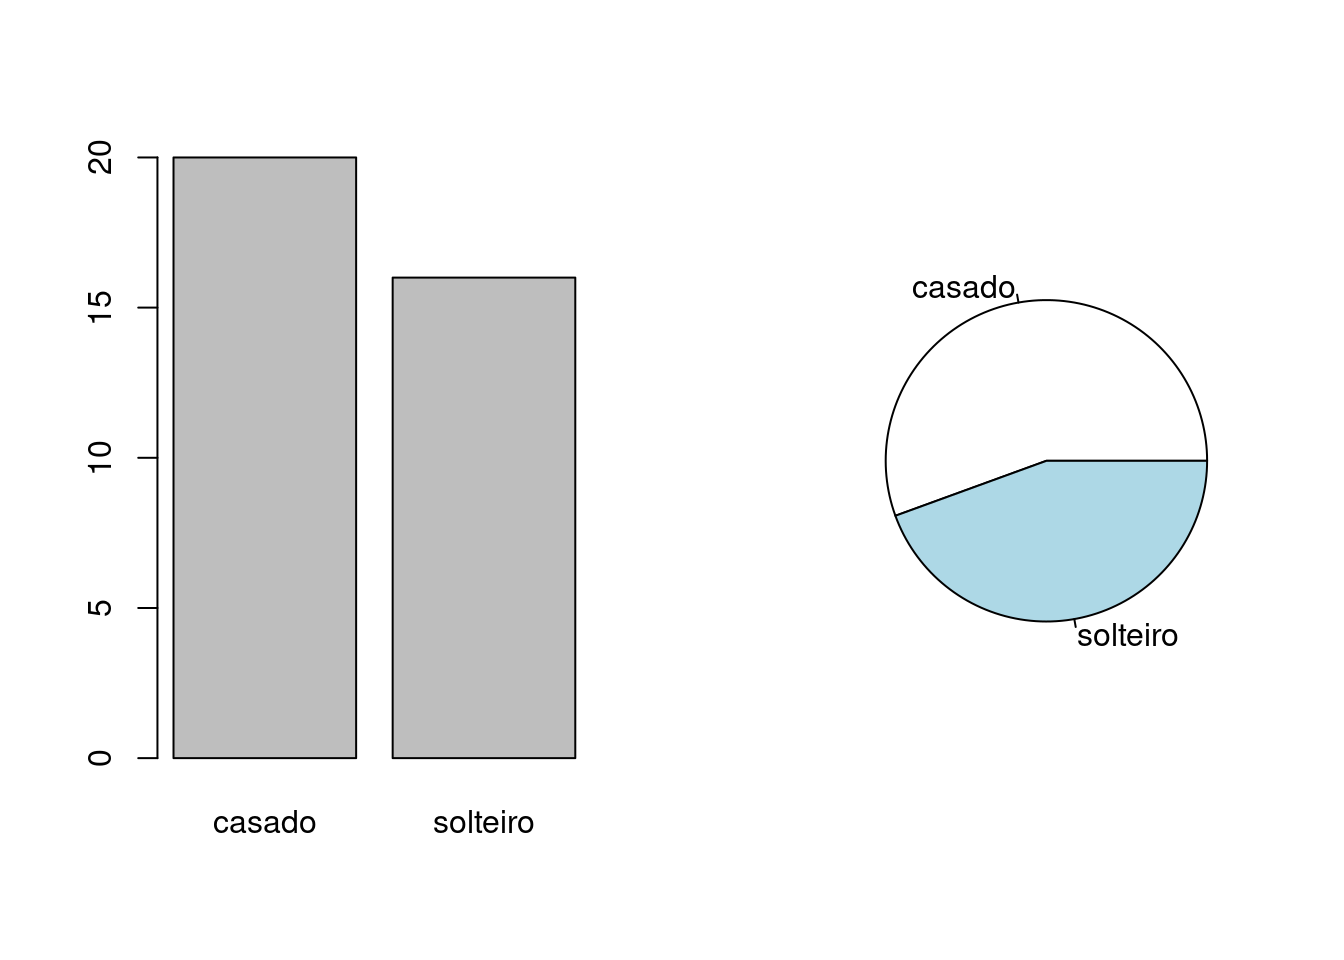
\includegraphics{figures/unnamed-chunk-293-1} \end{center}

A \emph{moda} de qualquer variável aleatória é definida como o valor mais
frequente encontrado na amostra. No R não há uma função pronta para
``calcular'' a moda, pois ela pode ser obtida facilmente através do uso de
funções básicas. Uma opção seria usar os comandos abaixo:

\begin{Shaded}
\begin{Highlighting}[]
\FunctionTok{names}\NormalTok{(civil.tb)[}\FunctionTok{which.max}\NormalTok{(civil.tb)]}
\NormalTok{[}\DecValTok{1}\NormalTok{] }\StringTok{"casado"}
\end{Highlighting}
\end{Shaded}

Deixamos a cargo do leitor entender e interpretar esse comando.

\hypertarget{variuxe1vel-qualitativa-ordinal}{%
\subsection{Variável Qualitativa Ordinal}\label{variuxe1vel-qualitativa-ordinal}}

Para exemplificar como obter análises para uma variável qualitativa
ordinal vamos selecionar a variável \texttt{Inst}.

As tabelas de frequências são obtidas de forma semelhante à mostrada
anteriormente.

\begin{Shaded}
\begin{Highlighting}[]
\DocumentationTok{\#\# Frequência absoluta}
\NormalTok{inst.tb }\OtherTok{\textless{}{-}} \FunctionTok{table}\NormalTok{(milsa}\SpecialCharTok{$}\NormalTok{Inst)}
\NormalTok{inst.tb}

\NormalTok{ 1o Grau  2o Grau Superior }
      \DecValTok{12}       \DecValTok{18}        \DecValTok{6} 
\DocumentationTok{\#\# Frequência relativa}
\FunctionTok{prop.table}\NormalTok{(inst.tb)}

\NormalTok{  1o Grau   2o Grau  Superior }
\FloatTok{0.3333333} \FloatTok{0.5000000} \FloatTok{0.1666667} 
\end{Highlighting}
\end{Shaded}

O gráfico de setores não é adequado para este tipo de variável por não
expressar a ordem dos possíveis valores. Usamos então apenas um gráfico
de barras conforme mostrado abaixo

\begin{Shaded}
\begin{Highlighting}[]
\FunctionTok{barplot}\NormalTok{(inst.tb)}
\end{Highlighting}
\end{Shaded}

\begin{center}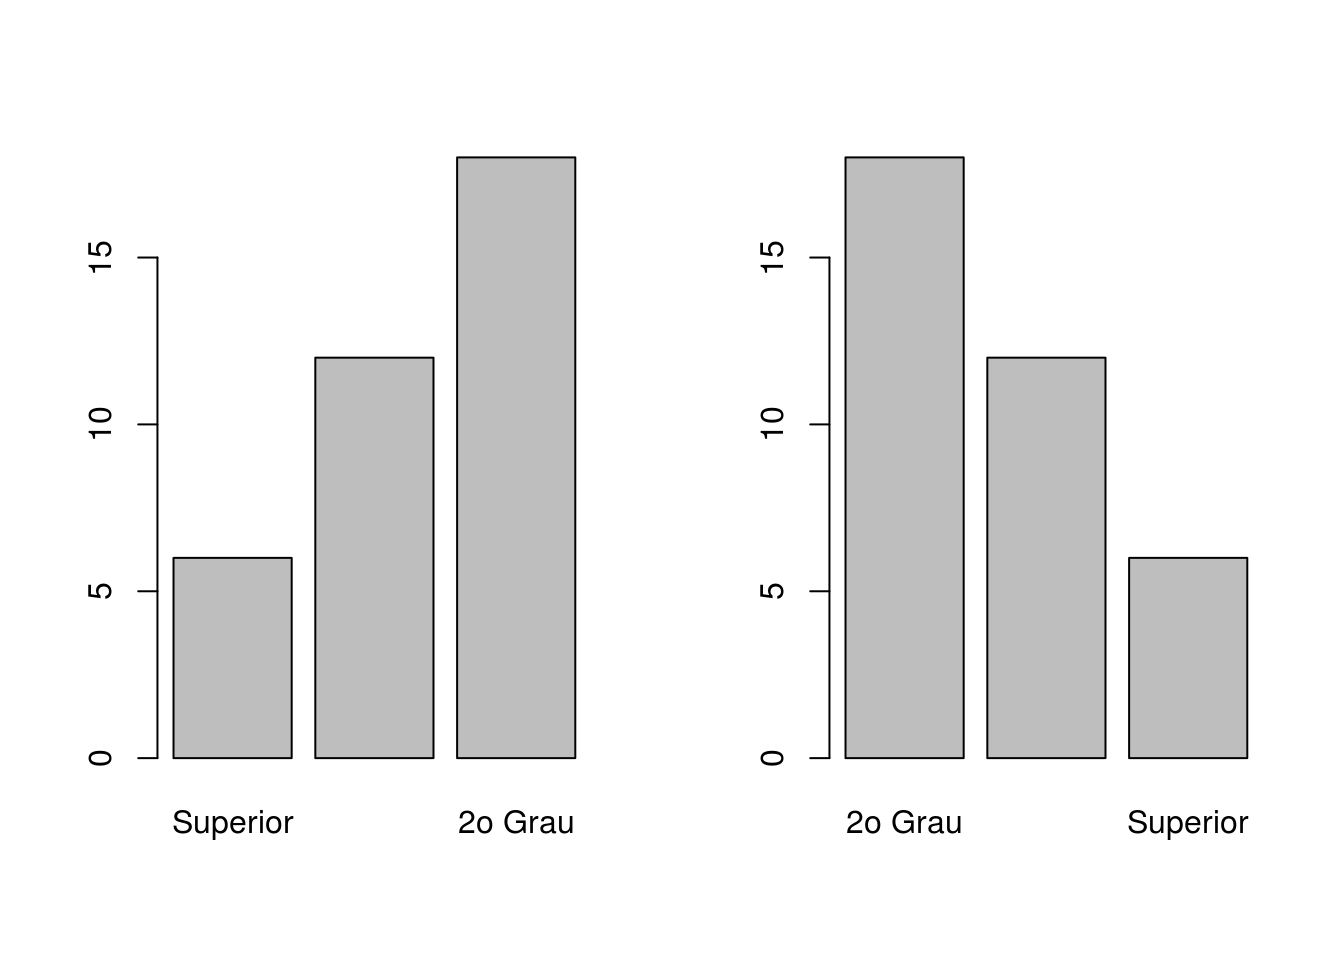
\includegraphics{figures/unnamed-chunk-296-1} \end{center}

Em alguns casos podemos querer mostrar o gráfico de barras com as barras
classificadas da menor para a maior, ou vice-versa, independente da
ordem dos níveis. Para isso podemos usar a função \texttt{sort()} para ordenar
os valores da tabela e fazer o gráfico

\begin{Shaded}
\begin{Highlighting}[]
\FunctionTok{par}\NormalTok{(}\AttributeTok{mfrow =} \FunctionTok{c}\NormalTok{(}\DecValTok{1}\NormalTok{,}\DecValTok{2}\NormalTok{))}
\DocumentationTok{\#\# Menor para maior}
\FunctionTok{barplot}\NormalTok{(}\FunctionTok{sort}\NormalTok{(inst.tb))}
\DocumentationTok{\#\# Maior para menor}
\FunctionTok{barplot}\NormalTok{(}\FunctionTok{sort}\NormalTok{(inst.tb, }\AttributeTok{decreasing =} \ConstantTok{TRUE}\NormalTok{))}
\FunctionTok{par}\NormalTok{(}\AttributeTok{mfrow =} \FunctionTok{c}\NormalTok{(}\DecValTok{1}\NormalTok{,}\DecValTok{1}\NormalTok{))}
\end{Highlighting}
\end{Shaded}

\begin{center}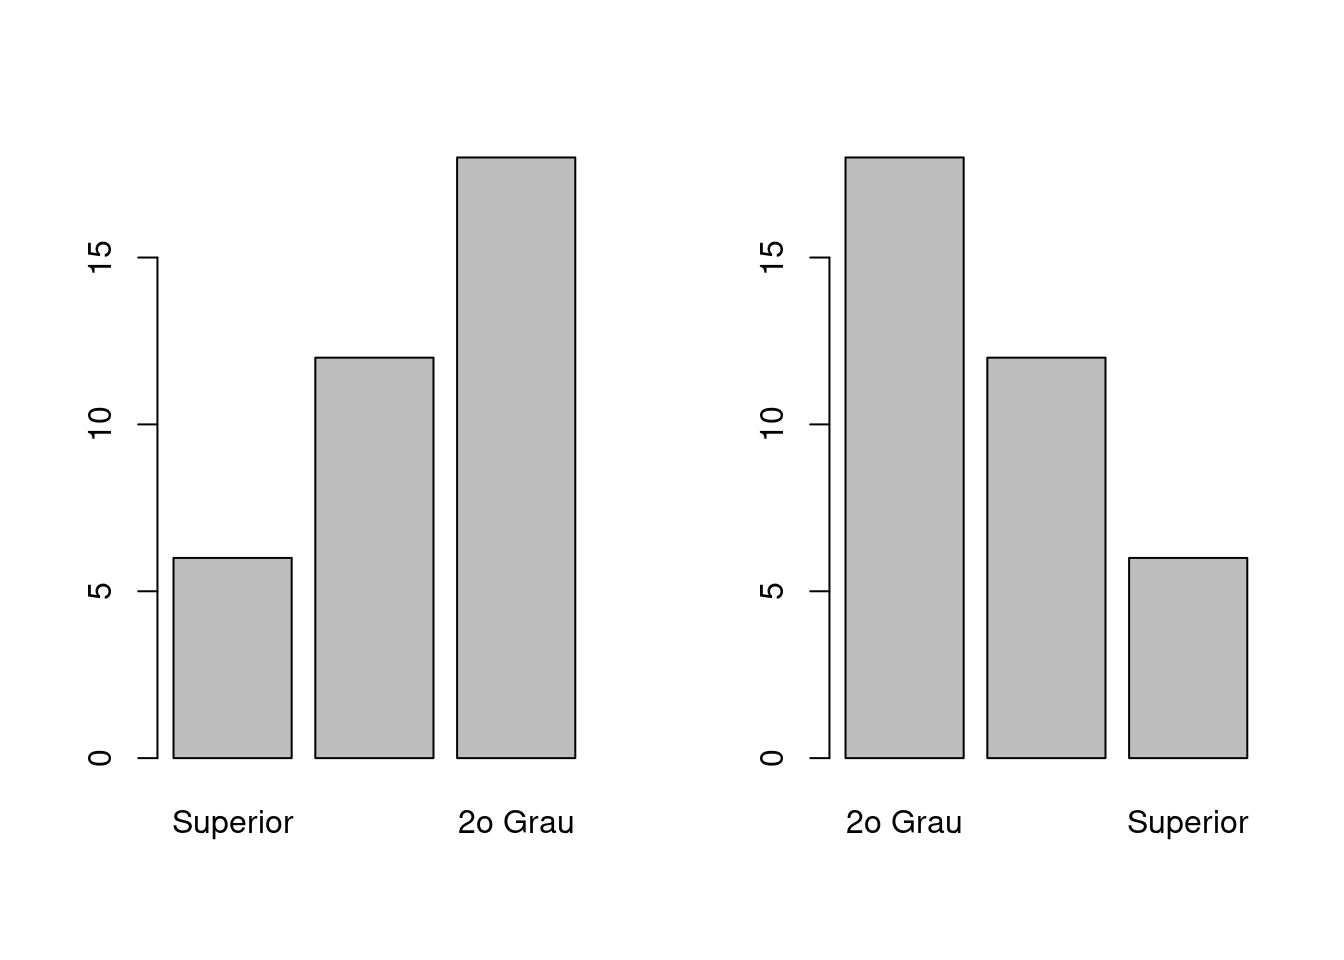
\includegraphics{figures/unnamed-chunk-297-1} \end{center}

Para uma variável ordinal, além da moda podemos também calcular outras
medidas, tais como a mediana conforme exemplificado a seguir. Note que
o comando \texttt{median()} não funciona com variáveis não numéricas, e por
isso usamos o comando seguinte.

\begin{Shaded}
\begin{Highlighting}[]
\DocumentationTok{\#\# Moda}
\FunctionTok{names}\NormalTok{(inst.tb)[}\FunctionTok{which.max}\NormalTok{(inst.tb)]}
\NormalTok{[}\DecValTok{1}\NormalTok{] }\StringTok{"2o Grau"}
\DocumentationTok{\#\# Mediana}
\FunctionTok{median}\NormalTok{(milsa}\SpecialCharTok{$}\NormalTok{Inst) }\CommentTok{\# só funciona para variáveis numéricas}
\NormalTok{Error }\ControlFlowTok{in} \FunctionTok{median.default}\NormalTok{(milsa}\SpecialCharTok{$}\NormalTok{Inst)}\SpecialCharTok{:}\NormalTok{ need numeric data}
\FunctionTok{median}\NormalTok{(}\FunctionTok{as.numeric}\NormalTok{(milsa}\SpecialCharTok{$}\NormalTok{Inst)) }\CommentTok{\# traz a mediana da codificação do nível}
\NormalTok{[}\DecValTok{1}\NormalTok{] }\DecValTok{2}
\FunctionTok{levels}\NormalTok{(milsa}\SpecialCharTok{$}\NormalTok{Inst)[}\FunctionTok{median}\NormalTok{(}\FunctionTok{as.numeric}\NormalTok{(milsa}\SpecialCharTok{$}\NormalTok{Inst))] }\CommentTok{\# valor correto}
\NormalTok{[}\DecValTok{1}\NormalTok{] }\StringTok{"2o Grau"}
\end{Highlighting}
\end{Shaded}

\hypertarget{variuxe1vel-quantitativa-discreta}{%
\subsection{Variável quantitativa discreta}\label{variuxe1vel-quantitativa-discreta}}

Vamos agora usar a variável \texttt{Filhos} (número de filhos) para
ilustrar algumas análises que podem ser feitas com uma quantitativa
discreta.

Frequências absolutas e relativas são obtidas como anteriormente. Também
vamos calcular a frequência acumulada, onde a frequência em uma classe é
a soma das frequências das classes anteriores. Para isso usamos a função
\texttt{cumsum()}, que já faz a soma acumulada.

\begin{Shaded}
\begin{Highlighting}[]
\DocumentationTok{\#\# Frequência absoluta}
\NormalTok{filhos.tb }\OtherTok{\textless{}{-}} \FunctionTok{table}\NormalTok{(milsa}\SpecialCharTok{$}\NormalTok{Filhos)}
\NormalTok{filhos.tb}

\DecValTok{0} \DecValTok{1} \DecValTok{2} \DecValTok{3} \DecValTok{5} 
\DecValTok{4} \DecValTok{5} \DecValTok{7} \DecValTok{3} \DecValTok{1} 
\DocumentationTok{\#\# Frequência relativa}
\NormalTok{filhos.tbr }\OtherTok{\textless{}{-}} \FunctionTok{prop.table}\NormalTok{(filhos.tb)}
\NormalTok{filhos.tbr}

   \DecValTok{0}    \DecValTok{1}    \DecValTok{2}    \DecValTok{3}    \DecValTok{5} 
\FloatTok{0.20} \FloatTok{0.25} \FloatTok{0.35} \FloatTok{0.15} \FloatTok{0.05} 
\DocumentationTok{\#\# Frequência acumulada}
\NormalTok{filhos.tba }\OtherTok{\textless{}{-}} \FunctionTok{cumsum}\NormalTok{(filhos.tbr)}
\NormalTok{filhos.tba}
   \DecValTok{0}    \DecValTok{1}    \DecValTok{2}    \DecValTok{3}    \DecValTok{5} 
\FloatTok{0.20} \FloatTok{0.45} \FloatTok{0.80} \FloatTok{0.95} \FloatTok{1.00} 
\end{Highlighting}
\end{Shaded}

O gráfico adequado para frequências absolutas de uma variável discreta é
parecido com um gráfico de barras, mas nesse caso, as frequências são
indicadas por linhas. Usando a função \texttt{plot()} em um objeto resultado da
função \texttt{table()}, o gráfico adequado já é selecionado:

\begin{Shaded}
\begin{Highlighting}[]
\FunctionTok{plot}\NormalTok{(filhos.tb)}
\end{Highlighting}
\end{Shaded}

\begin{center}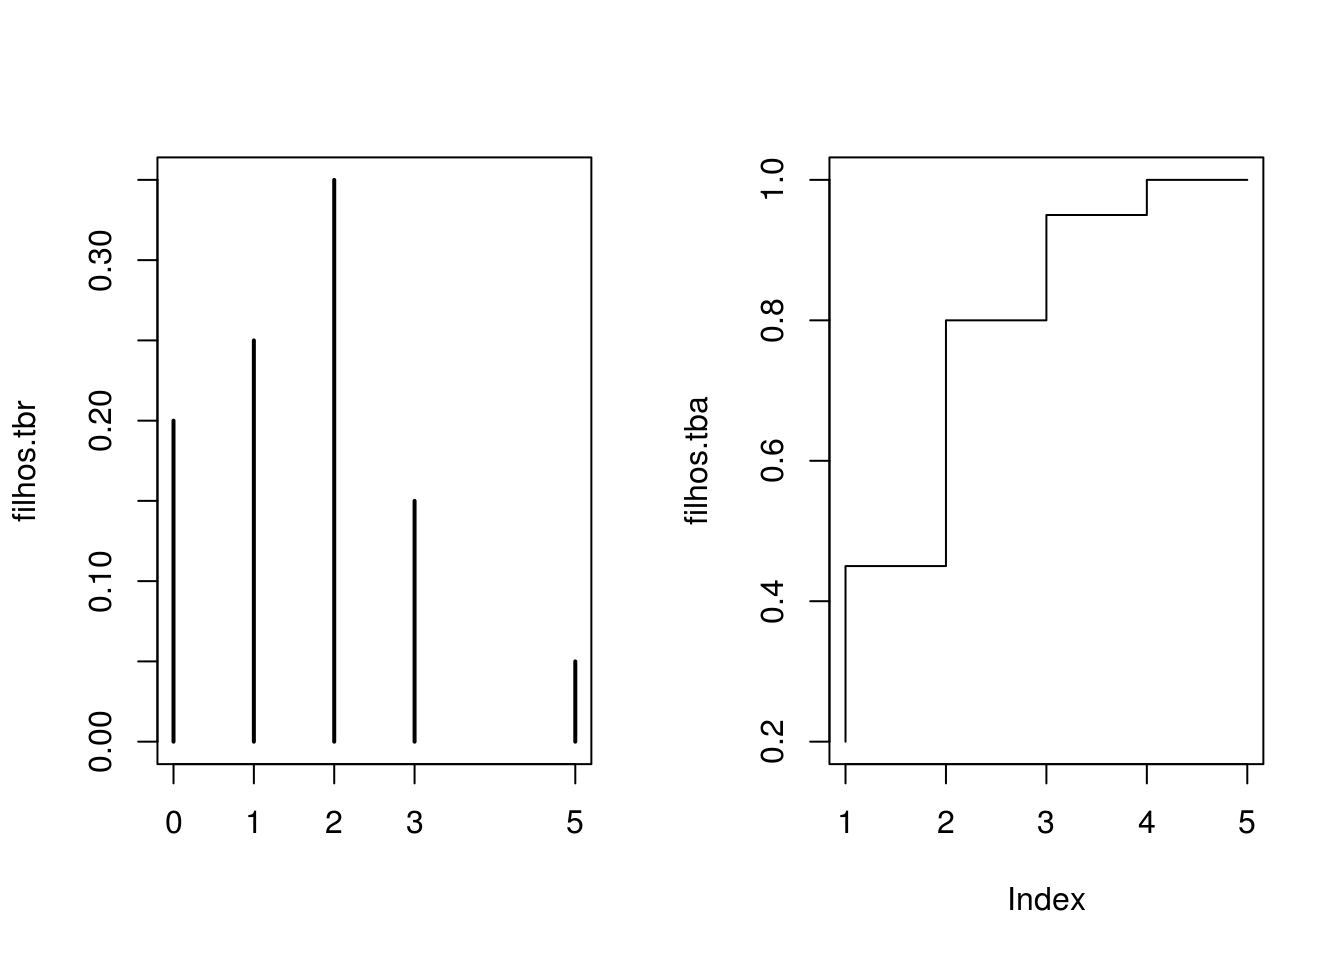
\includegraphics{figures/unnamed-chunk-300-1} \end{center}

Outra possibilidade seria fazer gráficos de frequências relativas e de
frequências acumuladas conforme mostrado na

\begin{Shaded}
\begin{Highlighting}[]
\FunctionTok{par}\NormalTok{(}\AttributeTok{mfrow =} \FunctionTok{c}\NormalTok{(}\DecValTok{1}\NormalTok{,}\DecValTok{2}\NormalTok{))}
\DocumentationTok{\#\# Frequência relativa}
\FunctionTok{plot}\NormalTok{(filhos.tbr)}
\DocumentationTok{\#\# Frequência relativa acumulada}
\FunctionTok{plot}\NormalTok{(filhos.tba, }\AttributeTok{type =} \StringTok{"S"}\NormalTok{) }\CommentTok{\# tipo step (escada)}
\FunctionTok{par}\NormalTok{(}\AttributeTok{mfrow =} \FunctionTok{c}\NormalTok{(}\DecValTok{1}\NormalTok{,}\DecValTok{1}\NormalTok{))}
\end{Highlighting}
\end{Shaded}

\begin{center}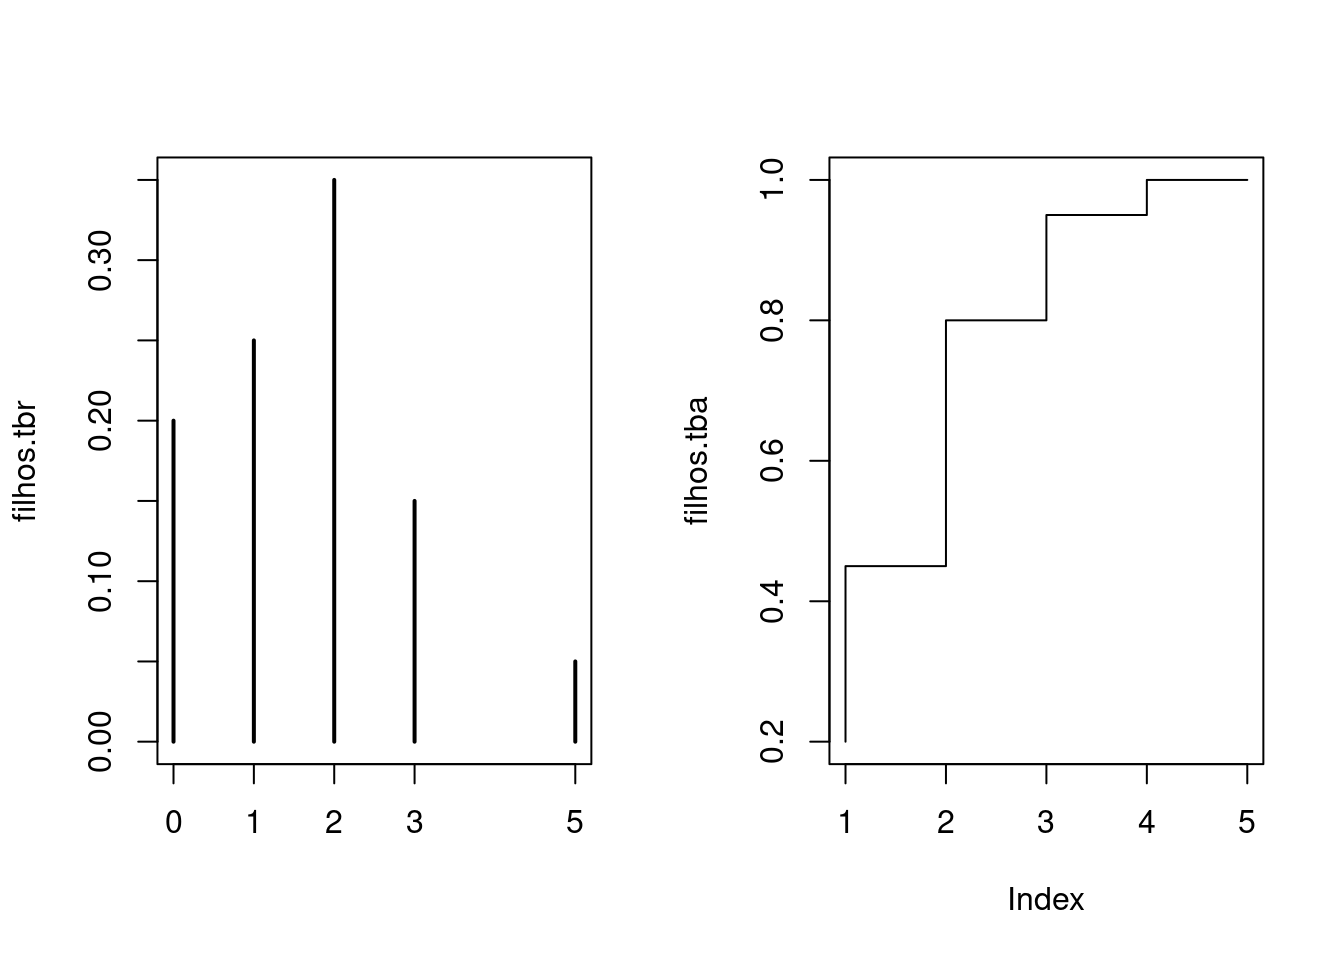
\includegraphics{figures/unnamed-chunk-301-1} \end{center}

Sendo a variável numérica há uma maior diversidade de medidas
estatísticas que podem ser calculadas.

A seguir mostramos como obter algumas medidas de posição: moda, mediana,
média e média aparada. Note que o argumento \texttt{na.rm\ =\ TRUE} é necessário
porque não há informação sobre número de filhos para alguns indivíduos
(\texttt{NA}). Para calcular a média aparada, usamos o argumento \texttt{trim\ =\ 0.1}
que indica que a média deve ser calculada excluindo-se 10\% dos menores e
10\% dos maiores valores do vetor de dados. Ao final mostramos como obter
os quartis, incluido o mínimo e o máximo.

\begin{Shaded}
\begin{Highlighting}[]
\DocumentationTok{\#\# Moda}
\FunctionTok{names}\NormalTok{(filhos.tb)[}\FunctionTok{which.max}\NormalTok{(filhos.tb)]}
\NormalTok{[}\DecValTok{1}\NormalTok{] }\StringTok{"2"}
\DocumentationTok{\#\# Mediana}
\FunctionTok{median}\NormalTok{(milsa}\SpecialCharTok{$}\NormalTok{Filhos, }\AttributeTok{na.rm =} \ConstantTok{TRUE}\NormalTok{)}
\NormalTok{[}\DecValTok{1}\NormalTok{] }\DecValTok{2}
\DocumentationTok{\#\# Média}
\FunctionTok{mean}\NormalTok{(milsa}\SpecialCharTok{$}\NormalTok{Filhos, }\AttributeTok{na.rm =} \ConstantTok{TRUE}\NormalTok{)}
\NormalTok{[}\DecValTok{1}\NormalTok{] }\FloatTok{1.65}
\DocumentationTok{\#\# Média aparada}
\FunctionTok{mean}\NormalTok{(milsa}\SpecialCharTok{$}\NormalTok{Filhos, }\AttributeTok{trim =} \FloatTok{0.1}\NormalTok{, }\AttributeTok{na.rm =} \ConstantTok{TRUE}\NormalTok{)}
\NormalTok{[}\DecValTok{1}\NormalTok{] }\FloatTok{1.5625}
\DocumentationTok{\#\# Quartis}
\FunctionTok{quantile}\NormalTok{(milsa}\SpecialCharTok{$}\NormalTok{Filhos, }\AttributeTok{na.rm =} \ConstantTok{TRUE}\NormalTok{)}
  \DecValTok{0}\SpecialCharTok{\%  25\%}  \DecValTok{50}\SpecialCharTok{\%  75\%} \DecValTok{100}\NormalTok{\% }
   \DecValTok{0}    \DecValTok{1}    \DecValTok{2}    \DecValTok{2}    \DecValTok{5} 
\end{Highlighting}
\end{Shaded}

Passando agora para medidas de dispersão, vejamos como obter o máximo e
mínimo, e com isso a amplitude, além da variância, desvio padrão, e
coeficiente de variação. Também obtemos os quartis para calcular a
amplitude interquartílica.

\begin{Shaded}
\begin{Highlighting}[]
\DocumentationTok{\#\# Máximo e mínimo}
\FunctionTok{max}\NormalTok{(milsa}\SpecialCharTok{$}\NormalTok{Filhos, }\AttributeTok{na.rm =} \ConstantTok{TRUE}\NormalTok{)}
\NormalTok{[}\DecValTok{1}\NormalTok{] }\DecValTok{5}
\FunctionTok{min}\NormalTok{(milsa}\SpecialCharTok{$}\NormalTok{Filhos, }\AttributeTok{na.rm =} \ConstantTok{TRUE}\NormalTok{)}
\NormalTok{[}\DecValTok{1}\NormalTok{] }\DecValTok{0}
\DocumentationTok{\#\# As duas informações juntas}
\FunctionTok{range}\NormalTok{(milsa}\SpecialCharTok{$}\NormalTok{Filhos, }\AttributeTok{na.rm =} \ConstantTok{TRUE}\NormalTok{)}
\NormalTok{[}\DecValTok{1}\NormalTok{] }\DecValTok{0} \DecValTok{5}
\DocumentationTok{\#\# Amplitude é a diferença entre máximo e mínimo}
\FunctionTok{diff}\NormalTok{(}\FunctionTok{range}\NormalTok{(milsa}\SpecialCharTok{$}\NormalTok{Filhos, }\AttributeTok{na.rm =} \ConstantTok{TRUE}\NormalTok{))}
\NormalTok{[}\DecValTok{1}\NormalTok{] }\DecValTok{5}
\DocumentationTok{\#\# Variância}
\FunctionTok{var}\NormalTok{(milsa}\SpecialCharTok{$}\NormalTok{Filhos, }\AttributeTok{na.rm =} \ConstantTok{TRUE}\NormalTok{)}
\NormalTok{[}\DecValTok{1}\NormalTok{] }\FloatTok{1.607895}
\DocumentationTok{\#\# Desvio{-}padrão}
\FunctionTok{sd}\NormalTok{(milsa}\SpecialCharTok{$}\NormalTok{Filhos, }\AttributeTok{na.rm =} \ConstantTok{TRUE}\NormalTok{)}
\NormalTok{[}\DecValTok{1}\NormalTok{] }\FloatTok{1.268028}
\DocumentationTok{\#\# Coeficiente de variação}
\FunctionTok{sd}\NormalTok{(milsa}\SpecialCharTok{$}\NormalTok{Filhos, }\AttributeTok{na.rm =} \ConstantTok{TRUE}\NormalTok{)}\SpecialCharTok{/}\FunctionTok{mean}\NormalTok{(milsa}\SpecialCharTok{$}\NormalTok{Filhos, }\AttributeTok{na.rm =} \ConstantTok{TRUE}\NormalTok{)}
\NormalTok{[}\DecValTok{1}\NormalTok{] }\FloatTok{0.7685018}
\DocumentationTok{\#\# Quartis}
\NormalTok{(filhos.qt }\OtherTok{\textless{}{-}} \FunctionTok{quantile}\NormalTok{(milsa}\SpecialCharTok{$}\NormalTok{Filhos, }\AttributeTok{na.rm =} \ConstantTok{TRUE}\NormalTok{))}
  \DecValTok{0}\SpecialCharTok{\%  25\%}  \DecValTok{50}\SpecialCharTok{\%  75\%} \DecValTok{100}\NormalTok{\% }
   \DecValTok{0}    \DecValTok{1}    \DecValTok{2}    \DecValTok{2}    \DecValTok{5} 
\DocumentationTok{\#\# Amplitude interquartílica}
\NormalTok{filhos.qt[}\DecValTok{4}\NormalTok{] }\SpecialCharTok{{-}}\NormalTok{ filhos.qt[}\DecValTok{2}\NormalTok{]}
\DecValTok{75}\NormalTok{\% }
  \DecValTok{1} 
\end{Highlighting}
\end{Shaded}

Finalmente, podemos usar a função \textbf{genérica} \texttt{summary()} para resumir
os dados de uma só vez

\begin{Shaded}
\begin{Highlighting}[]
\FunctionTok{summary}\NormalTok{(milsa}\SpecialCharTok{$}\NormalTok{Filhos)}
\NormalTok{   Min. 1st Qu.  Median    Mean 3rd Qu.    Max.    NA}\StringTok{\textquotesingle{}s }
\StringTok{   0.00    1.00    2.00    1.65    2.00    5.00      16 }
\end{Highlighting}
\end{Shaded}

\hypertarget{variuxe1vel-quantitativa-contuxednua}{%
\subsection{Variável quantitativa contínua}\label{variuxe1vel-quantitativa-contuxednua}}

Para concluir os exemplos para análise univariada vamos considerar a
variável quantitativa contínua \texttt{Salario}.

Para se fazer uma tabela de frequências de uma variável contínua, é preciso
primeiro agrupar os dados em classes. Nos comandos mostrados a seguir
verificamos inicialmente os valores máximo e mínimo dos dados, depois
usamos o critério de Sturges para definir o número de classes. Usamos
a função \texttt{cut()} para agrupar os dados em classes e finalmente obtemos
as frequências absolutas e relativas.

\begin{Shaded}
\begin{Highlighting}[]
\DocumentationTok{\#\# Máximo e mínimo}
\FunctionTok{range}\NormalTok{(milsa}\SpecialCharTok{$}\NormalTok{Salario)}
\NormalTok{[}\DecValTok{1}\NormalTok{]  }\FloatTok{4.0} \FloatTok{23.3}
\DocumentationTok{\#\# Número de classes estimado, com base no critério de Sturges. Veja}
\DocumentationTok{\#\# outras opções em ?nclass}
\FunctionTok{nclass.Sturges}\NormalTok{(milsa}\SpecialCharTok{$}\NormalTok{Salario)}
\NormalTok{[}\DecValTok{1}\NormalTok{] }\DecValTok{7}
\DocumentationTok{\#\# Criando as classes com a função cut(), usando os valores mínimos e}
\DocumentationTok{\#\# máximos dados em range()}
\FunctionTok{cut}\NormalTok{(milsa}\SpecialCharTok{$}\NormalTok{Salario, }\AttributeTok{breaks =} \FunctionTok{seq}\NormalTok{(}\DecValTok{4}\NormalTok{, }\FloatTok{23.3}\NormalTok{, }\AttributeTok{length.out =} \DecValTok{8}\NormalTok{))}
\NormalTok{ [}\DecValTok{1}\NormalTok{] }\SpecialCharTok{\textless{}}\ConstantTok{NA}\SpecialCharTok{\textgreater{}}\NormalTok{        (}\DecValTok{4}\NormalTok{,}\FloatTok{6.76}\NormalTok{]    (}\DecValTok{4}\NormalTok{,}\FloatTok{6.76}\NormalTok{]    (}\DecValTok{4}\NormalTok{,}\FloatTok{6.76}\NormalTok{]    (}\DecValTok{4}\NormalTok{,}\FloatTok{6.76}\NormalTok{]    (}\DecValTok{4}\NormalTok{,}\FloatTok{6.76}\NormalTok{]   }
\NormalTok{ [}\DecValTok{7}\NormalTok{] (}\FloatTok{6.76}\NormalTok{,}\FloatTok{9.51}\NormalTok{] (}\FloatTok{6.76}\NormalTok{,}\FloatTok{9.51}\NormalTok{] (}\FloatTok{6.76}\NormalTok{,}\FloatTok{9.51}\NormalTok{] (}\FloatTok{6.76}\NormalTok{,}\FloatTok{9.51}\NormalTok{] (}\FloatTok{6.76}\NormalTok{,}\FloatTok{9.51}\NormalTok{] (}\FloatTok{6.76}\NormalTok{,}\FloatTok{9.51}\NormalTok{]}
\NormalTok{[}\DecValTok{13}\NormalTok{] (}\FloatTok{6.76}\NormalTok{,}\FloatTok{9.51}\NormalTok{] (}\FloatTok{6.76}\NormalTok{,}\FloatTok{9.51}\NormalTok{] (}\FloatTok{6.76}\NormalTok{,}\FloatTok{9.51}\NormalTok{] (}\FloatTok{6.76}\NormalTok{,}\FloatTok{9.51}\NormalTok{] (}\FloatTok{9.51}\NormalTok{,}\FloatTok{12.3}\NormalTok{] (}\FloatTok{9.51}\NormalTok{,}\FloatTok{12.3}\NormalTok{]}
\NormalTok{[}\DecValTok{19}\NormalTok{] (}\FloatTok{9.51}\NormalTok{,}\FloatTok{12.3}\NormalTok{] (}\FloatTok{9.51}\NormalTok{,}\FloatTok{12.3}\NormalTok{] (}\FloatTok{9.51}\NormalTok{,}\FloatTok{12.3}\NormalTok{] (}\FloatTok{9.51}\NormalTok{,}\FloatTok{12.3}\NormalTok{] (}\FloatTok{9.51}\NormalTok{,}\FloatTok{12.3}\NormalTok{] (}\FloatTok{12.3}\NormalTok{,}\DecValTok{15}\NormalTok{]  }
\NormalTok{[}\DecValTok{25}\NormalTok{] (}\FloatTok{12.3}\NormalTok{,}\DecValTok{15}\NormalTok{]   (}\FloatTok{12.3}\NormalTok{,}\DecValTok{15}\NormalTok{]   (}\FloatTok{12.3}\NormalTok{,}\DecValTok{15}\NormalTok{]   (}\FloatTok{12.3}\NormalTok{,}\DecValTok{15}\NormalTok{]   (}\FloatTok{12.3}\NormalTok{,}\DecValTok{15}\NormalTok{]   (}\DecValTok{15}\NormalTok{,}\FloatTok{17.8}\NormalTok{]  }
\NormalTok{[}\DecValTok{31}\NormalTok{] (}\DecValTok{15}\NormalTok{,}\FloatTok{17.8}\NormalTok{]   (}\DecValTok{15}\NormalTok{,}\FloatTok{17.8}\NormalTok{]   (}\DecValTok{15}\NormalTok{,}\FloatTok{17.8}\NormalTok{]   (}\FloatTok{17.8}\NormalTok{,}\FloatTok{20.5}\NormalTok{] (}\FloatTok{17.8}\NormalTok{,}\FloatTok{20.5}\NormalTok{] (}\FloatTok{20.5}\NormalTok{,}\FloatTok{23.3}\NormalTok{]}
\DecValTok{7}\NormalTok{ Levels}\SpecialCharTok{:}\NormalTok{ (}\DecValTok{4}\NormalTok{,}\FloatTok{6.76}\NormalTok{] (}\FloatTok{6.76}\NormalTok{,}\FloatTok{9.51}\NormalTok{] (}\FloatTok{9.51}\NormalTok{,}\FloatTok{12.3}\NormalTok{] (}\FloatTok{12.3}\NormalTok{,}\DecValTok{15}\NormalTok{] (}\DecValTok{15}\NormalTok{,}\FloatTok{17.8}\NormalTok{] }\FunctionTok{...}\NormalTok{ (}\FloatTok{20.5}\NormalTok{,}\FloatTok{23.3}\NormalTok{]}
\end{Highlighting}
\end{Shaded}

Note que uma das classes é \texttt{NA}. Isso ocorre pela definição das classes,
que por padrão é no formato \texttt{(a,b{]}}, ou seja, o intervalo é aberto em
\texttt{a} (não inclui \texttt{a}) e fechado em \texttt{b} (inclui \texttt{b}). Podemos alterar esse
padrão usando o argumento \texttt{include.lowest\ =\ TRUE},

\begin{Shaded}
\begin{Highlighting}[]
\FunctionTok{cut}\NormalTok{(milsa}\SpecialCharTok{$}\NormalTok{Salario, }\AttributeTok{breaks =} \FunctionTok{seq}\NormalTok{(}\DecValTok{4}\NormalTok{, }\FloatTok{23.3}\NormalTok{, }\AttributeTok{length.out =} \DecValTok{8}\NormalTok{),}
    \AttributeTok{include.lowest =} \ConstantTok{TRUE}\NormalTok{)}
\NormalTok{ [}\DecValTok{1}\NormalTok{] [}\DecValTok{4}\NormalTok{,}\FloatTok{6.76}\NormalTok{]    [}\DecValTok{4}\NormalTok{,}\FloatTok{6.76}\NormalTok{]    [}\DecValTok{4}\NormalTok{,}\FloatTok{6.76}\NormalTok{]    [}\DecValTok{4}\NormalTok{,}\FloatTok{6.76}\NormalTok{]    [}\DecValTok{4}\NormalTok{,}\FloatTok{6.76}\NormalTok{]    [}\DecValTok{4}\NormalTok{,}\FloatTok{6.76}\NormalTok{]   }
\NormalTok{ [}\DecValTok{7}\NormalTok{] (}\FloatTok{6.76}\NormalTok{,}\FloatTok{9.51}\NormalTok{] (}\FloatTok{6.76}\NormalTok{,}\FloatTok{9.51}\NormalTok{] (}\FloatTok{6.76}\NormalTok{,}\FloatTok{9.51}\NormalTok{] (}\FloatTok{6.76}\NormalTok{,}\FloatTok{9.51}\NormalTok{] (}\FloatTok{6.76}\NormalTok{,}\FloatTok{9.51}\NormalTok{] (}\FloatTok{6.76}\NormalTok{,}\FloatTok{9.51}\NormalTok{]}
\NormalTok{[}\DecValTok{13}\NormalTok{] (}\FloatTok{6.76}\NormalTok{,}\FloatTok{9.51}\NormalTok{] (}\FloatTok{6.76}\NormalTok{,}\FloatTok{9.51}\NormalTok{] (}\FloatTok{6.76}\NormalTok{,}\FloatTok{9.51}\NormalTok{] (}\FloatTok{6.76}\NormalTok{,}\FloatTok{9.51}\NormalTok{] (}\FloatTok{9.51}\NormalTok{,}\FloatTok{12.3}\NormalTok{] (}\FloatTok{9.51}\NormalTok{,}\FloatTok{12.3}\NormalTok{]}
\NormalTok{[}\DecValTok{19}\NormalTok{] (}\FloatTok{9.51}\NormalTok{,}\FloatTok{12.3}\NormalTok{] (}\FloatTok{9.51}\NormalTok{,}\FloatTok{12.3}\NormalTok{] (}\FloatTok{9.51}\NormalTok{,}\FloatTok{12.3}\NormalTok{] (}\FloatTok{9.51}\NormalTok{,}\FloatTok{12.3}\NormalTok{] (}\FloatTok{9.51}\NormalTok{,}\FloatTok{12.3}\NormalTok{] (}\FloatTok{12.3}\NormalTok{,}\DecValTok{15}\NormalTok{]  }
\NormalTok{[}\DecValTok{25}\NormalTok{] (}\FloatTok{12.3}\NormalTok{,}\DecValTok{15}\NormalTok{]   (}\FloatTok{12.3}\NormalTok{,}\DecValTok{15}\NormalTok{]   (}\FloatTok{12.3}\NormalTok{,}\DecValTok{15}\NormalTok{]   (}\FloatTok{12.3}\NormalTok{,}\DecValTok{15}\NormalTok{]   (}\FloatTok{12.3}\NormalTok{,}\DecValTok{15}\NormalTok{]   (}\DecValTok{15}\NormalTok{,}\FloatTok{17.8}\NormalTok{]  }
\NormalTok{[}\DecValTok{31}\NormalTok{] (}\DecValTok{15}\NormalTok{,}\FloatTok{17.8}\NormalTok{]   (}\DecValTok{15}\NormalTok{,}\FloatTok{17.8}\NormalTok{]   (}\DecValTok{15}\NormalTok{,}\FloatTok{17.8}\NormalTok{]   (}\FloatTok{17.8}\NormalTok{,}\FloatTok{20.5}\NormalTok{] (}\FloatTok{17.8}\NormalTok{,}\FloatTok{20.5}\NormalTok{] (}\FloatTok{20.5}\NormalTok{,}\FloatTok{23.3}\NormalTok{]}
\DecValTok{7}\NormalTok{ Levels}\SpecialCharTok{:}\NormalTok{ [}\DecValTok{4}\NormalTok{,}\FloatTok{6.76}\NormalTok{] (}\FloatTok{6.76}\NormalTok{,}\FloatTok{9.51}\NormalTok{] (}\FloatTok{9.51}\NormalTok{,}\FloatTok{12.3}\NormalTok{] (}\FloatTok{12.3}\NormalTok{,}\DecValTok{15}\NormalTok{] (}\DecValTok{15}\NormalTok{,}\FloatTok{17.8}\NormalTok{] }\FunctionTok{...}\NormalTok{ (}\FloatTok{20.5}\NormalTok{,}\FloatTok{23.3}\NormalTok{]}
\end{Highlighting}
\end{Shaded}

E note que agora a primeira classe fica \texttt{{[}a,b{]}}, ou seja, fechada
(incluindo) os dois lados. Para que o intervalo seja fechado à esquerda,
usamos o argumento \texttt{right\ =\ FALSE}. As combinações possíveis para esses
dois argumentos, e as classes resultantes são apresentadas na tabela
abaixo:

\begin{longtable}[]{@{}cc@{}}
\toprule()
Argumentos & Resultado \\
\midrule()
\endhead
\texttt{include.lowest\ =\ T,\ right\ =\ T} & \texttt{{[}a,b{]},\ ...,\ (y,z{]}} \\
\texttt{include.lowest\ =\ F,\ right\ =\ T} & \texttt{(a,b{]},\ ...,\ (y,z{]}} \\
\texttt{include.lowest\ =\ F,\ right\ =\ F} & \texttt{{[}a,b),\ ...,\ {[}y,z)} \\
\texttt{include.lowest\ =\ T,\ right\ =\ F} & \texttt{{[}a,b),\ ...,\ {[}y,z{]}} \\
\bottomrule()
\end{longtable}

Outra opção para ``acomodar'' todos os extremos dentro das classes, seria
naturalmente atribuir valores um pouco menores que o mínimo, e um pouco
maiores que o máximo. Abaixo, usamos essa abordagem e fazemos uma tabela
com as frequências absolutas e relativas.

\begin{Shaded}
\begin{Highlighting}[]
\NormalTok{salario.cut }\OtherTok{\textless{}{-}} \FunctionTok{cut}\NormalTok{(milsa}\SpecialCharTok{$}\NormalTok{Salario,}
                   \AttributeTok{breaks =} \FunctionTok{seq}\NormalTok{(}\FloatTok{3.5}\NormalTok{, }\FloatTok{23.5}\NormalTok{, }\AttributeTok{length.out =} \DecValTok{8}\NormalTok{))}
\NormalTok{salario.cut}
\NormalTok{ [}\DecValTok{1}\NormalTok{] (}\FloatTok{3.5}\NormalTok{,}\FloatTok{6.36}\NormalTok{]  (}\FloatTok{3.5}\NormalTok{,}\FloatTok{6.36}\NormalTok{]  (}\FloatTok{3.5}\NormalTok{,}\FloatTok{6.36}\NormalTok{]  (}\FloatTok{3.5}\NormalTok{,}\FloatTok{6.36}\NormalTok{]  (}\FloatTok{3.5}\NormalTok{,}\FloatTok{6.36}\NormalTok{]  (}\FloatTok{6.36}\NormalTok{,}\FloatTok{9.21}\NormalTok{]}
\NormalTok{ [}\DecValTok{7}\NormalTok{] (}\FloatTok{6.36}\NormalTok{,}\FloatTok{9.21}\NormalTok{] (}\FloatTok{6.36}\NormalTok{,}\FloatTok{9.21}\NormalTok{] (}\FloatTok{6.36}\NormalTok{,}\FloatTok{9.21}\NormalTok{] (}\FloatTok{6.36}\NormalTok{,}\FloatTok{9.21}\NormalTok{] (}\FloatTok{6.36}\NormalTok{,}\FloatTok{9.21}\NormalTok{] (}\FloatTok{6.36}\NormalTok{,}\FloatTok{9.21}\NormalTok{]}
\NormalTok{[}\DecValTok{13}\NormalTok{] (}\FloatTok{6.36}\NormalTok{,}\FloatTok{9.21}\NormalTok{] (}\FloatTok{6.36}\NormalTok{,}\FloatTok{9.21}\NormalTok{] (}\FloatTok{6.36}\NormalTok{,}\FloatTok{9.21}\NormalTok{] (}\FloatTok{9.21}\NormalTok{,}\FloatTok{12.1}\NormalTok{] (}\FloatTok{9.21}\NormalTok{,}\FloatTok{12.1}\NormalTok{] (}\FloatTok{9.21}\NormalTok{,}\FloatTok{12.1}\NormalTok{]}
\NormalTok{[}\DecValTok{19}\NormalTok{] (}\FloatTok{9.21}\NormalTok{,}\FloatTok{12.1}\NormalTok{] (}\FloatTok{9.21}\NormalTok{,}\FloatTok{12.1}\NormalTok{] (}\FloatTok{9.21}\NormalTok{,}\FloatTok{12.1}\NormalTok{] (}\FloatTok{9.21}\NormalTok{,}\FloatTok{12.1}\NormalTok{] (}\FloatTok{9.21}\NormalTok{,}\FloatTok{12.1}\NormalTok{] (}\FloatTok{12.1}\NormalTok{,}\FloatTok{14.9}\NormalTok{]}
\NormalTok{[}\DecValTok{25}\NormalTok{] (}\FloatTok{12.1}\NormalTok{,}\FloatTok{14.9}\NormalTok{] (}\FloatTok{12.1}\NormalTok{,}\FloatTok{14.9}\NormalTok{] (}\FloatTok{12.1}\NormalTok{,}\FloatTok{14.9}\NormalTok{] (}\FloatTok{12.1}\NormalTok{,}\FloatTok{14.9}\NormalTok{] (}\FloatTok{12.1}\NormalTok{,}\FloatTok{14.9}\NormalTok{] (}\FloatTok{14.9}\NormalTok{,}\FloatTok{17.8}\NormalTok{]}
\NormalTok{[}\DecValTok{31}\NormalTok{] (}\FloatTok{14.9}\NormalTok{,}\FloatTok{17.8}\NormalTok{] (}\FloatTok{14.9}\NormalTok{,}\FloatTok{17.8}\NormalTok{] (}\FloatTok{14.9}\NormalTok{,}\FloatTok{17.8}\NormalTok{] (}\FloatTok{17.8}\NormalTok{,}\FloatTok{20.6}\NormalTok{] (}\FloatTok{17.8}\NormalTok{,}\FloatTok{20.6}\NormalTok{] (}\FloatTok{20.6}\NormalTok{,}\FloatTok{23.5}\NormalTok{]}
\DecValTok{7}\NormalTok{ Levels}\SpecialCharTok{:}\NormalTok{ (}\FloatTok{3.5}\NormalTok{,}\FloatTok{6.36}\NormalTok{] (}\FloatTok{6.36}\NormalTok{,}\FloatTok{9.21}\NormalTok{] (}\FloatTok{9.21}\NormalTok{,}\FloatTok{12.1}\NormalTok{] (}\FloatTok{12.1}\NormalTok{,}\FloatTok{14.9}\NormalTok{] }\FunctionTok{...}\NormalTok{ (}\FloatTok{20.6}\NormalTok{,}\FloatTok{23.5}\NormalTok{]}
\DocumentationTok{\#\# Tabela com as frequencias absolutas por classe}
\NormalTok{salario.tb }\OtherTok{\textless{}{-}} \FunctionTok{table}\NormalTok{(salario.cut)}
\NormalTok{salario.tb}
\NormalTok{salario.cut}
\NormalTok{ (}\FloatTok{3.5}\NormalTok{,}\FloatTok{6.36}\NormalTok{] (}\FloatTok{6.36}\NormalTok{,}\FloatTok{9.21}\NormalTok{] (}\FloatTok{9.21}\NormalTok{,}\FloatTok{12.1}\NormalTok{] (}\FloatTok{12.1}\NormalTok{,}\FloatTok{14.9}\NormalTok{] (}\FloatTok{14.9}\NormalTok{,}\FloatTok{17.8}\NormalTok{] (}\FloatTok{17.8}\NormalTok{,}\FloatTok{20.6}\NormalTok{] }
          \DecValTok{5}          \DecValTok{10}           \DecValTok{8}           \DecValTok{6}           \DecValTok{4}           \DecValTok{2} 
\NormalTok{(}\FloatTok{20.6}\NormalTok{,}\FloatTok{23.5}\NormalTok{] }
          \DecValTok{1} 
\DocumentationTok{\#\# Tabela com as frequências relativas}
\FunctionTok{prop.table}\NormalTok{(salario.tb)}
\NormalTok{salario.cut}
\NormalTok{ (}\FloatTok{3.5}\NormalTok{,}\FloatTok{6.36}\NormalTok{] (}\FloatTok{6.36}\NormalTok{,}\FloatTok{9.21}\NormalTok{] (}\FloatTok{9.21}\NormalTok{,}\FloatTok{12.1}\NormalTok{] (}\FloatTok{12.1}\NormalTok{,}\FloatTok{14.9}\NormalTok{] (}\FloatTok{14.9}\NormalTok{,}\FloatTok{17.8}\NormalTok{] (}\FloatTok{17.8}\NormalTok{,}\FloatTok{20.6}\NormalTok{] }
 \FloatTok{0.13888889}  \FloatTok{0.27777778}  \FloatTok{0.22222222}  \FloatTok{0.16666667}  \FloatTok{0.11111111}  \FloatTok{0.05555556} 
\NormalTok{(}\FloatTok{20.6}\NormalTok{,}\FloatTok{23.5}\NormalTok{] }
 \FloatTok{0.02777778} 
\end{Highlighting}
\end{Shaded}

Na sequência vamos mostrar dois possíveis gráficos para variáveis
contínuas: o histograma e o \emph{box-plot}.

Para fazer um histograma usamos a função \texttt{hist()}, por exemplo,

\begin{Shaded}
\begin{Highlighting}[]
\FunctionTok{hist}\NormalTok{(milsa}\SpecialCharTok{$}\NormalTok{Salario)}
\end{Highlighting}
\end{Shaded}

\begin{center}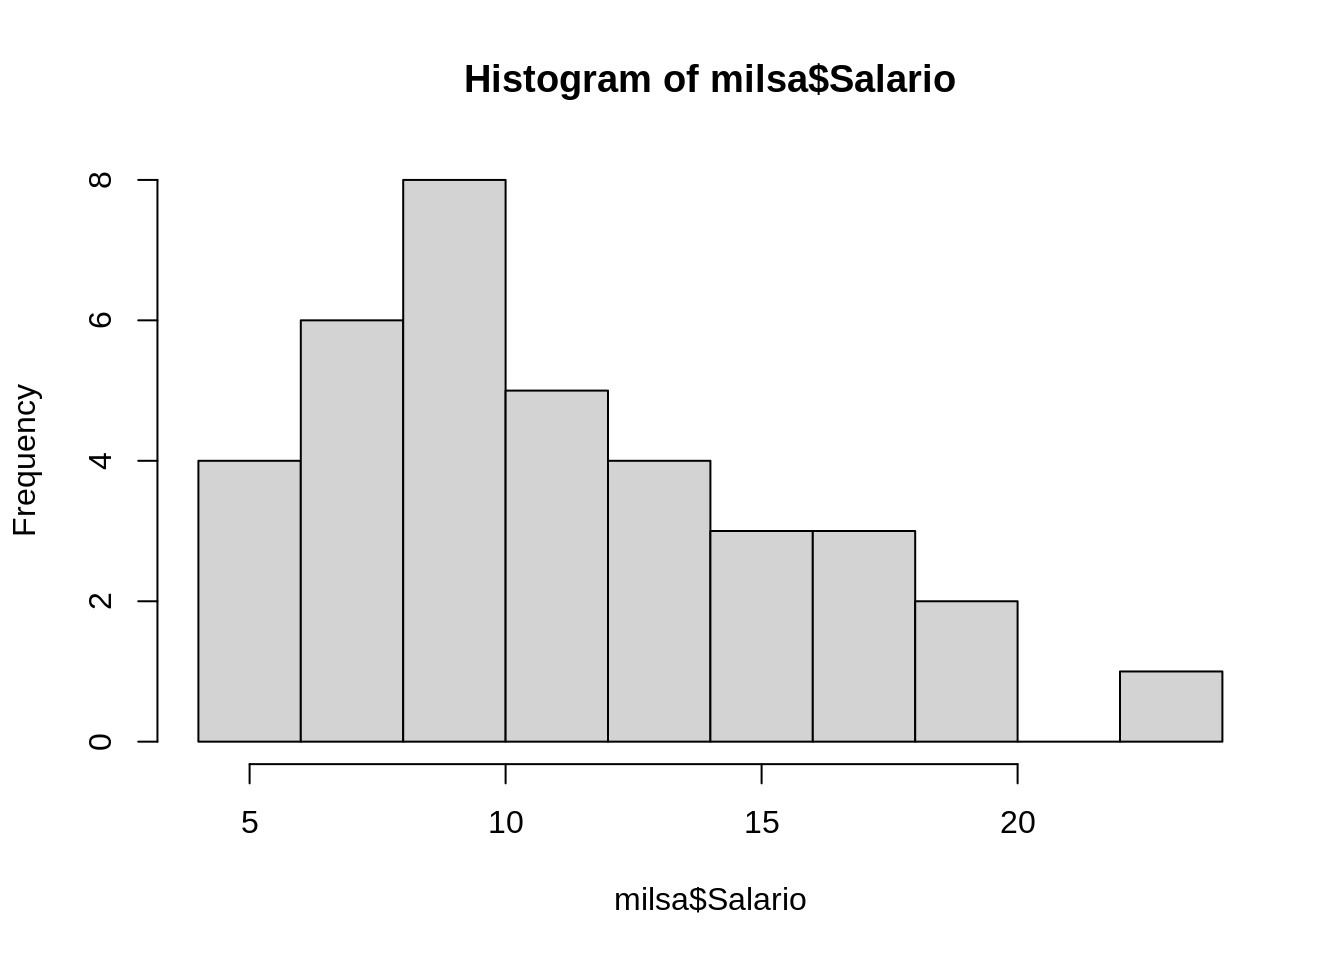
\includegraphics{figures/unnamed-chunk-308-1} \end{center}

A função \texttt{hist()} possui vários argumentos para alterar o comportamento
da saída do gráfico. Por exemplo, com \texttt{labels\ =\ TRUE} as frequências são
mostradas acima de cada barra. Com \texttt{freq\ =\ FALSE}, o gráfico é feito com
as frequências relativas.

\begin{Shaded}
\begin{Highlighting}[]
\FunctionTok{hist}\NormalTok{(milsa}\SpecialCharTok{$}\NormalTok{Salario, }\AttributeTok{freq =} \ConstantTok{FALSE}\NormalTok{, }\AttributeTok{labels =} \ConstantTok{TRUE}\NormalTok{)}
\end{Highlighting}
\end{Shaded}

\begin{center}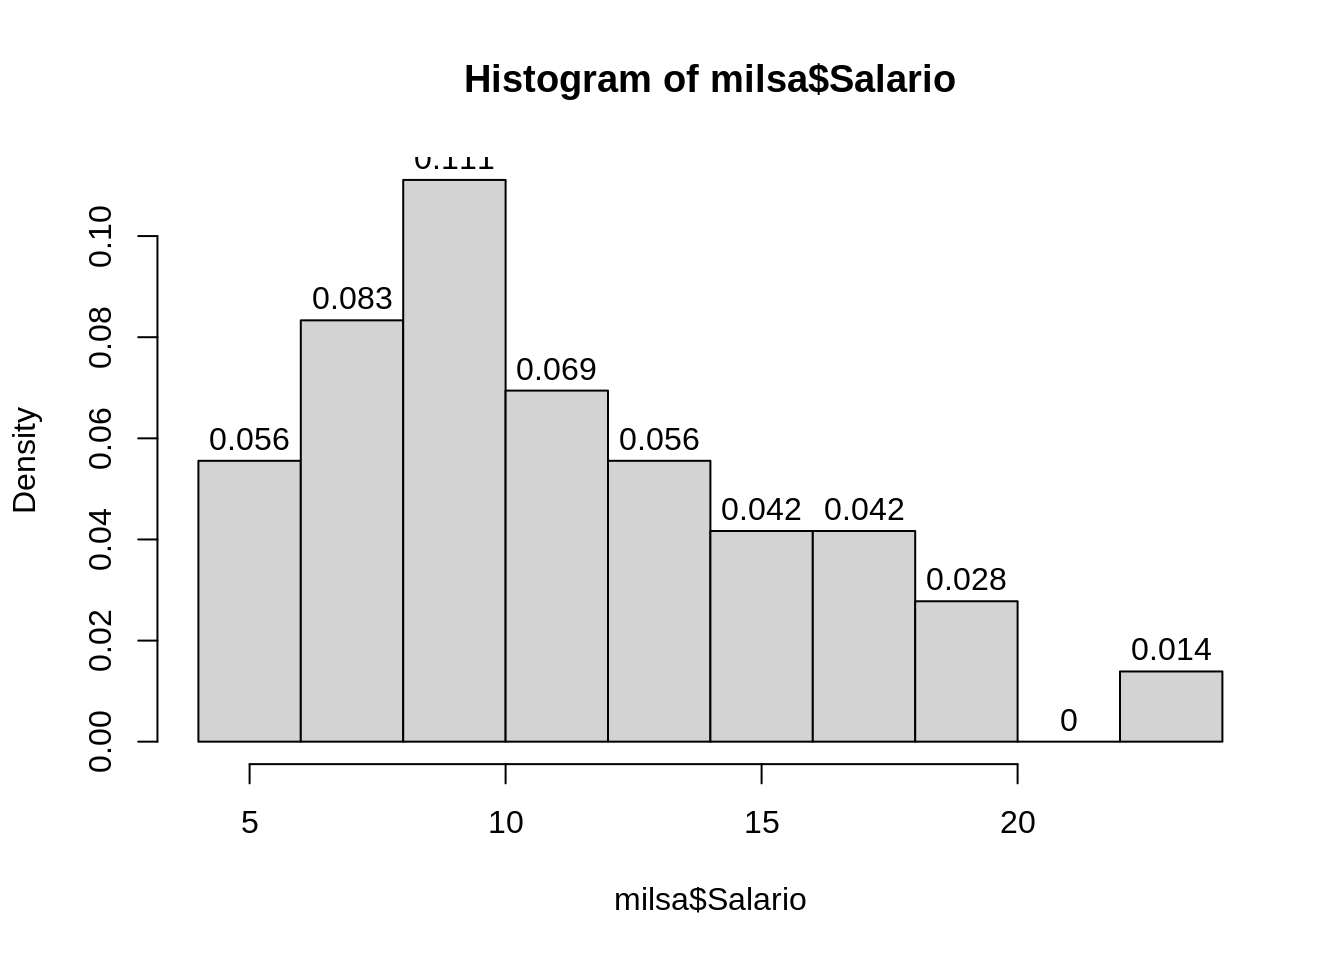
\includegraphics{figures/unnamed-chunk-309-1} \end{center}

Por padrão, a função \texttt{hist()} calcula automaticamente o número de
classes e os valores limites de cada classe. No entanto, isto pode ser
alterado com o argumento \texttt{breaks}, que pode receber um vetor
definindo os limites das classes, uma função para definir as quebras, um
nome de critério (por exemplo, \texttt{"Sturges"}), ou um único escalar
definido o número de classes. As últimas três opções são apenas
sugestões utilizadas pela função. O argumento \texttt{nclass} também funciona
dessa forma, recebendo apenas um valor com o número de classes (como
sugestão).

\begin{Shaded}
\begin{Highlighting}[]
\FunctionTok{hist}\NormalTok{(milsa}\SpecialCharTok{$}\NormalTok{Salario, }\AttributeTok{nclass =} \DecValTok{15}\NormalTok{)}
\end{Highlighting}
\end{Shaded}

\begin{center}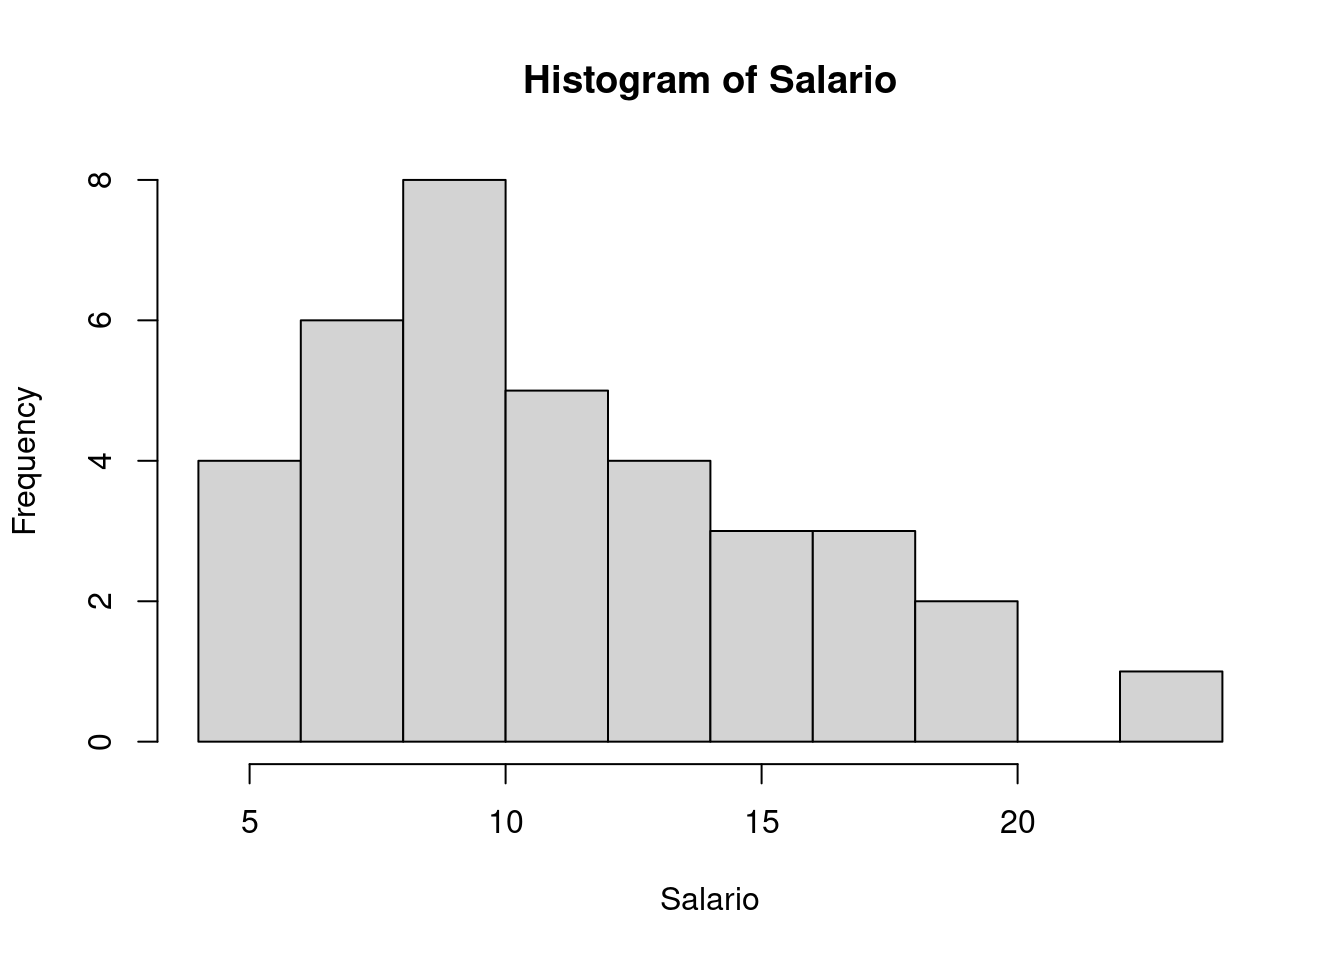
\includegraphics{figures/unnamed-chunk-310-1} \end{center}

Assim como na função \texttt{cut()}, os argumentos \texttt{include.lowest} e \texttt{right}
são utilizados para controlar a borda das classes.

Uma característica importante da função \texttt{hist()} é que ela retorna não
apenas o gráfico, mas também uma lista com as informações utilizadas
para construir o gráfico. Associando um histograma a um objeto, podemos
ver o seu conteúdo:

\begin{Shaded}
\begin{Highlighting}[]
\NormalTok{salario.hist }\OtherTok{\textless{}{-}} \FunctionTok{hist}\NormalTok{(milsa}\SpecialCharTok{$}\NormalTok{Salario)}
\end{Highlighting}
\end{Shaded}

\begin{center}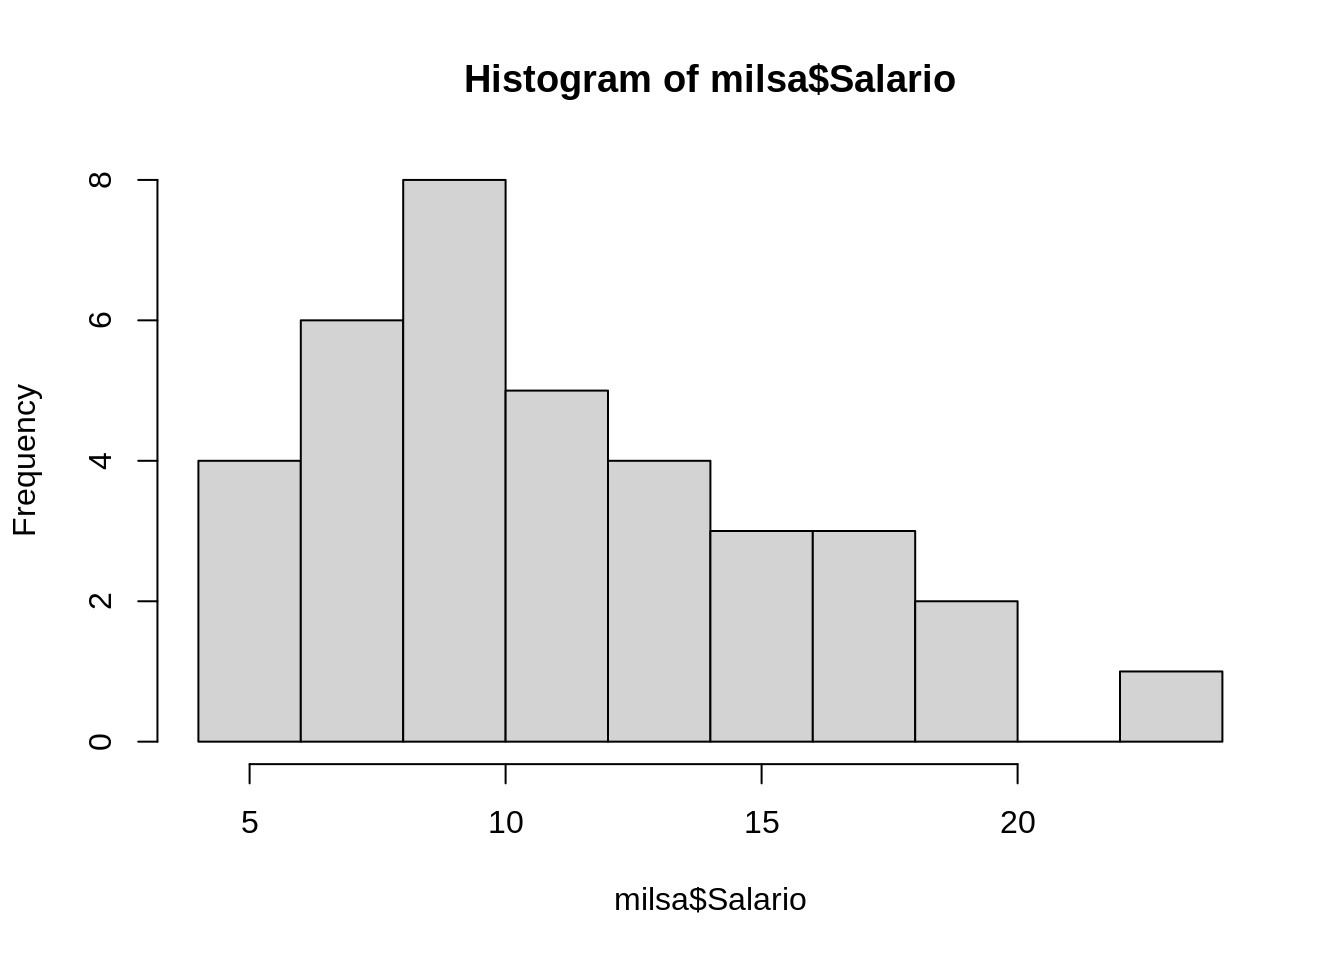
\includegraphics{figures/unnamed-chunk-311-1} \end{center}

\begin{Shaded}
\begin{Highlighting}[]
\NormalTok{salario.hist}
\SpecialCharTok{$}\NormalTok{breaks}
\NormalTok{ [}\DecValTok{1}\NormalTok{]  }\DecValTok{4}  \DecValTok{6}  \DecValTok{8} \DecValTok{10} \DecValTok{12} \DecValTok{14} \DecValTok{16} \DecValTok{18} \DecValTok{20} \DecValTok{22} \DecValTok{24}

\SpecialCharTok{$}\NormalTok{counts}
\NormalTok{ [}\DecValTok{1}\NormalTok{] }\DecValTok{4} \DecValTok{6} \DecValTok{8} \DecValTok{5} \DecValTok{4} \DecValTok{3} \DecValTok{3} \DecValTok{2} \DecValTok{0} \DecValTok{1}

\SpecialCharTok{$}\NormalTok{density}
\NormalTok{ [}\DecValTok{1}\NormalTok{] }\FloatTok{0.05555556} \FloatTok{0.08333333} \FloatTok{0.11111111} \FloatTok{0.06944444} \FloatTok{0.05555556} \FloatTok{0.04166667}
\NormalTok{ [}\DecValTok{7}\NormalTok{] }\FloatTok{0.04166667} \FloatTok{0.02777778} \FloatTok{0.00000000} \FloatTok{0.01388889}

\SpecialCharTok{$}\NormalTok{mids}
\NormalTok{ [}\DecValTok{1}\NormalTok{]  }\DecValTok{5}  \DecValTok{7}  \DecValTok{9} \DecValTok{11} \DecValTok{13} \DecValTok{15} \DecValTok{17} \DecValTok{19} \DecValTok{21} \DecValTok{23}

\SpecialCharTok{$}\NormalTok{xname}
\NormalTok{[}\DecValTok{1}\NormalTok{] }\StringTok{"milsa$Salario"}

\SpecialCharTok{$}\NormalTok{equidist}
\NormalTok{[}\DecValTok{1}\NormalTok{] }\ConstantTok{TRUE}

\FunctionTok{attr}\NormalTok{(,}\StringTok{"class"}\NormalTok{)}
\NormalTok{[}\DecValTok{1}\NormalTok{] }\StringTok{"histogram"}
\end{Highlighting}
\end{Shaded}

Estas informações podem então ser utilizadas para outros propósitos
dentro do R.

Os \textbf{boxplots} são úteis para revelar o centro, a dispersão e a
distribuição dos dados, além de \textbf{outliers}. São construídos da
seguinte forma:

\begin{itemize}
\tightlist
\item
  A linha central mais escura representa a mediana. Os extremos da
  caixa são o \(1^{o}\) (\(q1\)) e o \(3^{o}\) (\(q3\)) quartis.
\item
  As linhas que se extendem das caixas são definidas como:
  \[q1-1,5\cdot IQR\ \qquad \mathrm{e}\ \qquad q3+1,5\cdot IQR\]
  onde \(IQR\) é o intervalo inter-quartil. As linhas vão até os valores
  máximo e mínimo que ainda se encontram dentro deste intervalo.
\end{itemize}

\begin{Shaded}
\begin{Highlighting}[]
\FunctionTok{boxplot}\NormalTok{(milsa}\SpecialCharTok{$}\NormalTok{Salario)}
\end{Highlighting}
\end{Shaded}

\begin{center}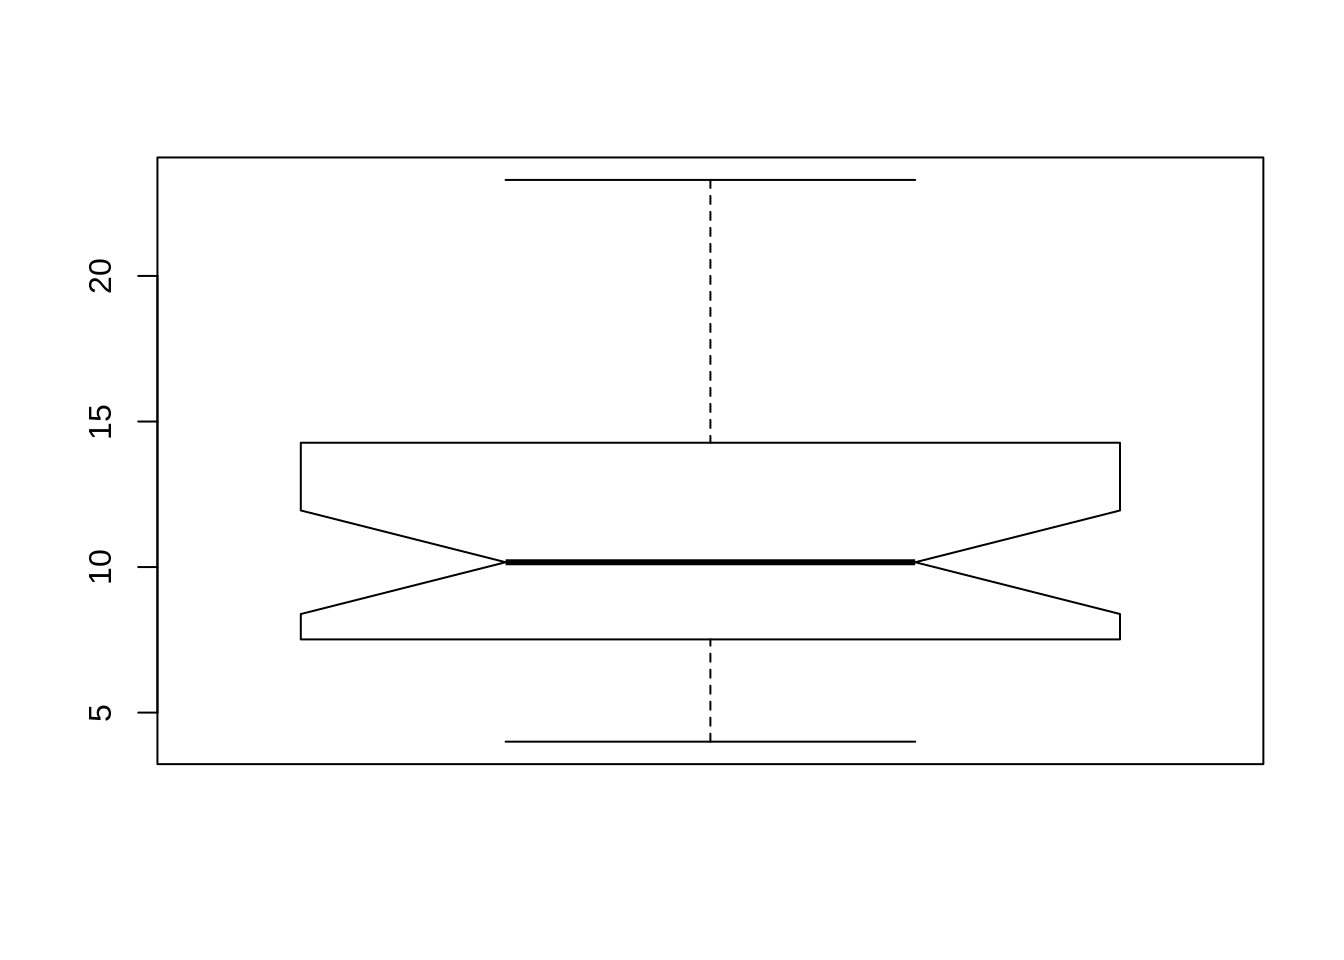
\includegraphics{figures/unnamed-chunk-312-1} \end{center}

Existem também vários argumentos que permitem variações do \emph{boxplot},
tais como caixas com tamanho proporcional aos tamanhos
dos grupos (\texttt{varwidth\ =\ TRUE}), e caixas ``acinturadas'' (\emph{notched
boxplot}) (\texttt{notch\ =\ TRUE}).

\begin{Shaded}
\begin{Highlighting}[]
\FunctionTok{boxplot}\NormalTok{(milsa}\SpecialCharTok{$}\NormalTok{Salario, }\AttributeTok{varwidth =} \ConstantTok{TRUE}\NormalTok{, }\AttributeTok{notch =} \ConstantTok{TRUE}\NormalTok{)}
\end{Highlighting}
\end{Shaded}

\begin{center}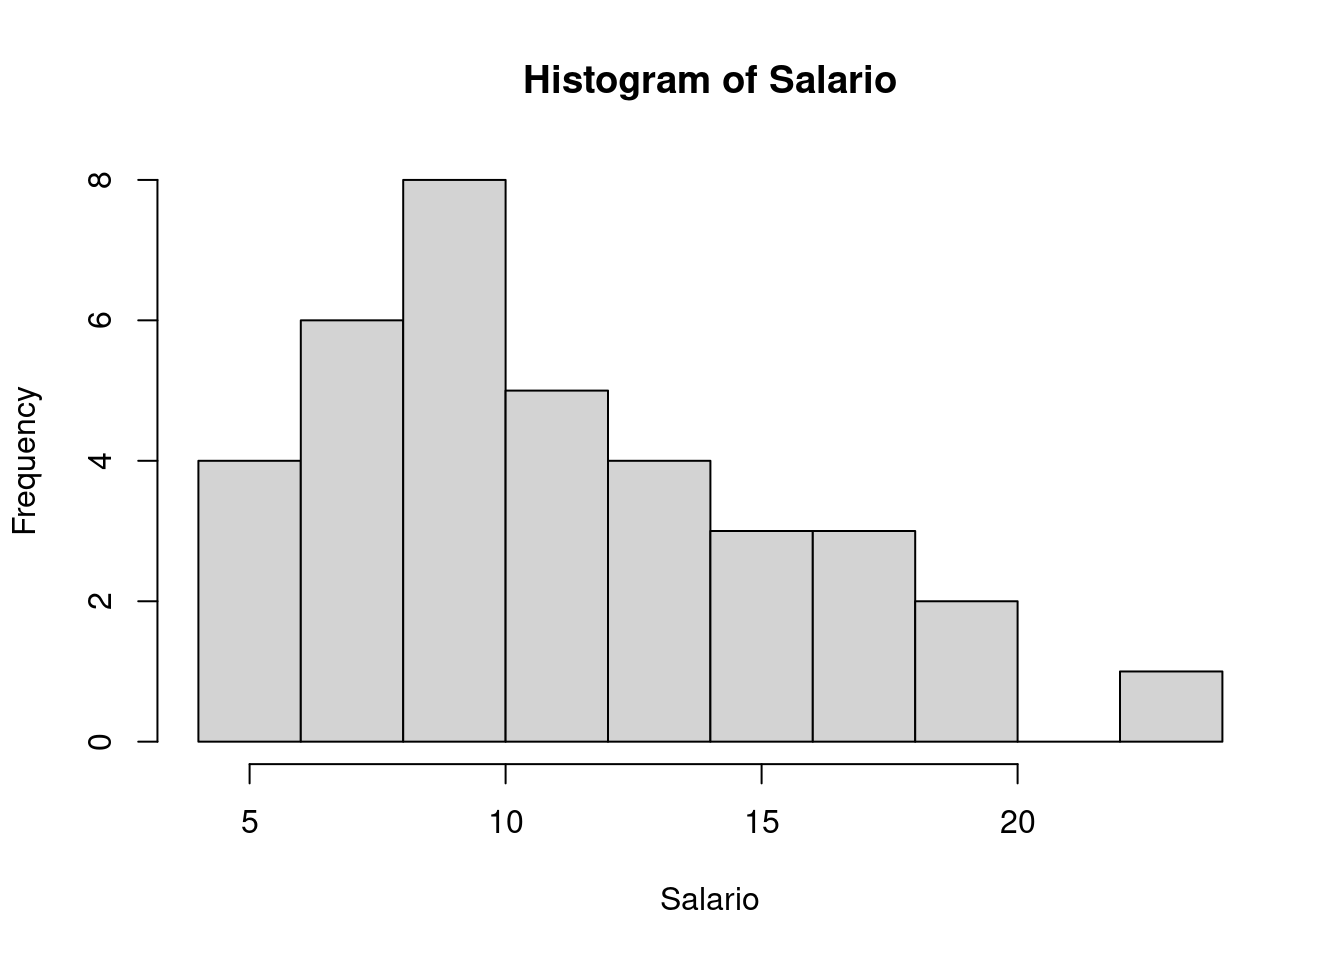
\includegraphics{figures/unnamed-chunk-313-1} \end{center}

Ambas opções são úteis quando há mais de um grupo e a comparação entre
os boxplots é facilitada.

Finalmente, podemos obter as medidas de posição e dispersão da mesma
forma que para variáveis discretas. Veja alguns exemplos a seguir. Note
que aqui não é necessário o uso do argumento \texttt{na.rm\ =\ TRUE}, pois não
existem \texttt{NA}s nesta variável.

\begin{Shaded}
\begin{Highlighting}[]
\DocumentationTok{\#\# Mediana}
\FunctionTok{median}\NormalTok{(milsa}\SpecialCharTok{$}\NormalTok{Salario)}
\NormalTok{[}\DecValTok{1}\NormalTok{] }\FloatTok{10.165}
\DocumentationTok{\#\# Média}
\FunctionTok{mean}\NormalTok{(milsa}\SpecialCharTok{$}\NormalTok{Salario)}
\NormalTok{[}\DecValTok{1}\NormalTok{] }\FloatTok{11.12222}
\DocumentationTok{\#\# Média aparada}
\FunctionTok{mean}\NormalTok{(milsa}\SpecialCharTok{$}\NormalTok{Salario, }\AttributeTok{trim =} \FloatTok{0.1}\NormalTok{)}
\NormalTok{[}\DecValTok{1}\NormalTok{] }\FloatTok{10.838}
\DocumentationTok{\#\# Quartis}
\FunctionTok{quantile}\NormalTok{(milsa}\SpecialCharTok{$}\NormalTok{Salario)}
     \DecValTok{0}\SpecialCharTok{\%     25\%}     \DecValTok{50}\SpecialCharTok{\%     75\%}    \DecValTok{100}\NormalTok{\% }
 \FloatTok{4.0000}  \FloatTok{7.5525} \FloatTok{10.1650} \FloatTok{14.0600} \FloatTok{23.3000} 
\DocumentationTok{\#\# Máximo e mínimo}
\FunctionTok{max}\NormalTok{(milsa}\SpecialCharTok{$}\NormalTok{Salario)}
\NormalTok{[}\DecValTok{1}\NormalTok{] }\FloatTok{23.3}
\FunctionTok{min}\NormalTok{(milsa}\SpecialCharTok{$}\NormalTok{Salario)}
\NormalTok{[}\DecValTok{1}\NormalTok{] }\DecValTok{4}
\DocumentationTok{\#\# As duas informações juntas}
\FunctionTok{range}\NormalTok{(milsa}\SpecialCharTok{$}\NormalTok{Salario)}
\NormalTok{[}\DecValTok{1}\NormalTok{]  }\FloatTok{4.0} \FloatTok{23.3}
\DocumentationTok{\#\# Amplitude é a diferença entre máximo e mínimo}
\FunctionTok{diff}\NormalTok{(}\FunctionTok{range}\NormalTok{(milsa}\SpecialCharTok{$}\NormalTok{Salario))}
\NormalTok{[}\DecValTok{1}\NormalTok{] }\FloatTok{19.3}
\DocumentationTok{\#\# Variância}
\FunctionTok{var}\NormalTok{(milsa}\SpecialCharTok{$}\NormalTok{Salario)}
\NormalTok{[}\DecValTok{1}\NormalTok{] }\FloatTok{21.04477}
\DocumentationTok{\#\# Desvio{-}padrão}
\FunctionTok{sd}\NormalTok{(milsa}\SpecialCharTok{$}\NormalTok{Salario)}
\NormalTok{[}\DecValTok{1}\NormalTok{] }\FloatTok{4.587458}
\DocumentationTok{\#\# Coeficiente de variação}
\FunctionTok{sd}\NormalTok{(milsa}\SpecialCharTok{$}\NormalTok{Salario)}\SpecialCharTok{/}\FunctionTok{mean}\NormalTok{(milsa}\SpecialCharTok{$}\NormalTok{Salario)}
\NormalTok{[}\DecValTok{1}\NormalTok{] }\FloatTok{0.4124587}
\DocumentationTok{\#\# Quartis}
\NormalTok{salario.qt }\OtherTok{\textless{}{-}} \FunctionTok{quantile}\NormalTok{(milsa}\SpecialCharTok{$}\NormalTok{Salario)}
\DocumentationTok{\#\# Amplitude interquartílica}
\NormalTok{salario.qt[}\DecValTok{4}\NormalTok{] }\SpecialCharTok{{-}}\NormalTok{ salario.qt[}\DecValTok{2}\NormalTok{]}
   \DecValTok{75}\NormalTok{\% }
\FloatTok{6.5075} 
\end{Highlighting}
\end{Shaded}

\hypertarget{anuxe1lise-bivariada}{%
\section{Análise Bivariada}\label{anuxe1lise-bivariada}}

Na análise bivariada procuramos identificar relações entre duas variáveis.
Assim como na análise univariada, estas relações podem ser resumidas por
gráficos, tabelas e/ou medidas estatísticas.
O tipo de resumo vai depender dos tipos das variáveis envolvidas.
Vamos considerar três possibilidades:

\begin{itemize}
\tightlist
\item
  Qualitativa \emph{vs} qualitativa
\item
  Qualitativa \emph{vs} quantitativa
\item
  Quantitativa \emph{vs} quantitativa
\end{itemize}

Salienta-se ainda que:

\begin{itemize}
\tightlist
\item
  As análise mostradas a seguir não esgotam as possibilidades de
  análises envolvendo duas variáveis e devem ser vistas apenas como uma
  sugestão inicial.
\item
  Relações entre duas variáveis devem ser examinadas com cautela pois
  podem ser mascaradas por uma ou mais variáveis adicionais não
  considerada na análise. Estas são chamadas \textbf{variáveis de
  confundimento}. Análises com variáveis de confundimento não serão
  discutidas neste ponto.
\end{itemize}

\begin{quote}
\textbf{Observação}: de agora em diante, como serão consideradas mais de
uma variável, usaremos a função \texttt{with()} para chamar a maioria das
funções.
\end{quote}

\hypertarget{qualitativa-vs-qualitativa}{%
\subsection{\texorpdfstring{Qualitativa \emph{vs} qualitativa}{Qualitativa vs qualitativa}}\label{qualitativa-vs-qualitativa}}

Vamos considerar as variáveis \texttt{Est.civil} (estado civil), e \texttt{Inst} (grau
de instrução). A tabela envolvendo duas variáveis é chamada \textbf{tabela de
cruzamento} ou \textbf{tabela de contingência}, e pode ser apresentada de
várias formas, conforme discutido a seguir.

A forma adequada de apresentação vai depender dos objetivos da análise e
da interpretação desejada para os dados. Inicialmente obtemos a tabela de
frequências absolutas para o cruzamento das duas variáveis, usando a
função \texttt{table()}. A tabela extendida incluindo os totais marginais pode
ser obtida com a função \texttt{addmargins()}.

\begin{Shaded}
\begin{Highlighting}[]
\DocumentationTok{\#\# Tabela de frequências absolutas}
\NormalTok{civ.inst.tb }\OtherTok{\textless{}{-}} \FunctionTok{with}\NormalTok{(milsa, }\FunctionTok{table}\NormalTok{(Est.civil, Inst))}
\NormalTok{civ.inst.tb}
\NormalTok{          Inst}
\NormalTok{Est.civil  1o Grau 2o Grau Superior}
\NormalTok{  casado         }\DecValTok{5}      \DecValTok{12}        \DecValTok{3}
\NormalTok{  solteiro       }\DecValTok{7}       \DecValTok{6}        \DecValTok{3}
\FunctionTok{addmargins}\NormalTok{(civ.inst.tb)}
\NormalTok{          Inst}
\NormalTok{Est.civil  1o Grau 2o Grau Superior Sum}
\NormalTok{  casado         }\DecValTok{5}      \DecValTok{12}        \DecValTok{3}  \DecValTok{20}
\NormalTok{  solteiro       }\DecValTok{7}       \DecValTok{6}        \DecValTok{3}  \DecValTok{16}
\NormalTok{  Sum           }\DecValTok{12}      \DecValTok{18}        \DecValTok{6}  \DecValTok{36}
\end{Highlighting}
\end{Shaded}

Tabelas de frequências relativas são obtidas com \texttt{prop.table()}, mas
aqui existem três possibilidades para as proporções em cada casela:

\begin{itemize}
\tightlist
\item
  Em relação ao total geral.
\item
  Em relação aos totais por linha (\texttt{margin\ =\ 1}).
\item
  Em relação aos totais por coluna (\texttt{margin\ =\ 2}).
\end{itemize}

\begin{Shaded}
\begin{Highlighting}[]
\DocumentationTok{\#\# Frequência relativa global}
\FunctionTok{prop.table}\NormalTok{(civ.inst.tb)}
\NormalTok{          Inst}
\NormalTok{Est.civil     1o Grau    2o Grau   Superior}
\NormalTok{  casado   }\FloatTok{0.13888889} \FloatTok{0.33333333} \FloatTok{0.08333333}
\NormalTok{  solteiro }\FloatTok{0.19444444} \FloatTok{0.16666667} \FloatTok{0.08333333}
\DocumentationTok{\#\# Frequência relativa por linha}
\FunctionTok{prop.table}\NormalTok{(civ.inst.tb, }\AttributeTok{margin =} \DecValTok{1}\NormalTok{)}
\NormalTok{          Inst}
\NormalTok{Est.civil  1o Grau 2o Grau Superior}
\NormalTok{  casado    }\FloatTok{0.2500}  \FloatTok{0.6000}   \FloatTok{0.1500}
\NormalTok{  solteiro  }\FloatTok{0.4375}  \FloatTok{0.3750}   \FloatTok{0.1875}
\DocumentationTok{\#\# Frequência relativa por coluna}
\FunctionTok{prop.table}\NormalTok{(civ.inst.tb, }\AttributeTok{margin =} \DecValTok{2}\NormalTok{)}
\NormalTok{          Inst}
\NormalTok{Est.civil    1o Grau   2o Grau  Superior}
\NormalTok{  casado   }\FloatTok{0.4166667} \FloatTok{0.6666667} \FloatTok{0.5000000}
\NormalTok{  solteiro }\FloatTok{0.5833333} \FloatTok{0.3333333} \FloatTok{0.5000000}
\end{Highlighting}
\end{Shaded}

Abaixo são representados quatro tipos de gráficos de barras que podem
ser usados para representar o cruzamento das variáveis. A transposição
da tabela com \texttt{t()} permite alterar a variável que define os grupos no
eixo horizontal. O uso de \texttt{prop.table()} permite o obtenção de gráficos
com frequências relativas.

\begin{Shaded}
\begin{Highlighting}[]
\FunctionTok{par}\NormalTok{(}\AttributeTok{mfrow =} \FunctionTok{c}\NormalTok{(}\DecValTok{2}\NormalTok{,}\DecValTok{2}\NormalTok{))}
\FunctionTok{barplot}\NormalTok{(civ.inst.tb, }\AttributeTok{legend =} \ConstantTok{TRUE}\NormalTok{)}
\FunctionTok{barplot}\NormalTok{(}\FunctionTok{t}\NormalTok{(civ.inst.tb), }\AttributeTok{legend =} \ConstantTok{TRUE}\NormalTok{)}
\FunctionTok{barplot}\NormalTok{(civ.inst.tb, }\AttributeTok{beside =} \ConstantTok{TRUE}\NormalTok{, }\AttributeTok{legend =} \ConstantTok{TRUE}\NormalTok{)}
\FunctionTok{barplot}\NormalTok{(}\FunctionTok{t}\NormalTok{(}\FunctionTok{prop.table}\NormalTok{(civ.inst.tb)), }\AttributeTok{beside =} \ConstantTok{TRUE}\NormalTok{, }\AttributeTok{legend =} \ConstantTok{TRUE}\NormalTok{)}
\FunctionTok{par}\NormalTok{(}\AttributeTok{mfrow =} \FunctionTok{c}\NormalTok{(}\DecValTok{1}\NormalTok{,}\DecValTok{1}\NormalTok{))}
\end{Highlighting}
\end{Shaded}

\begin{center}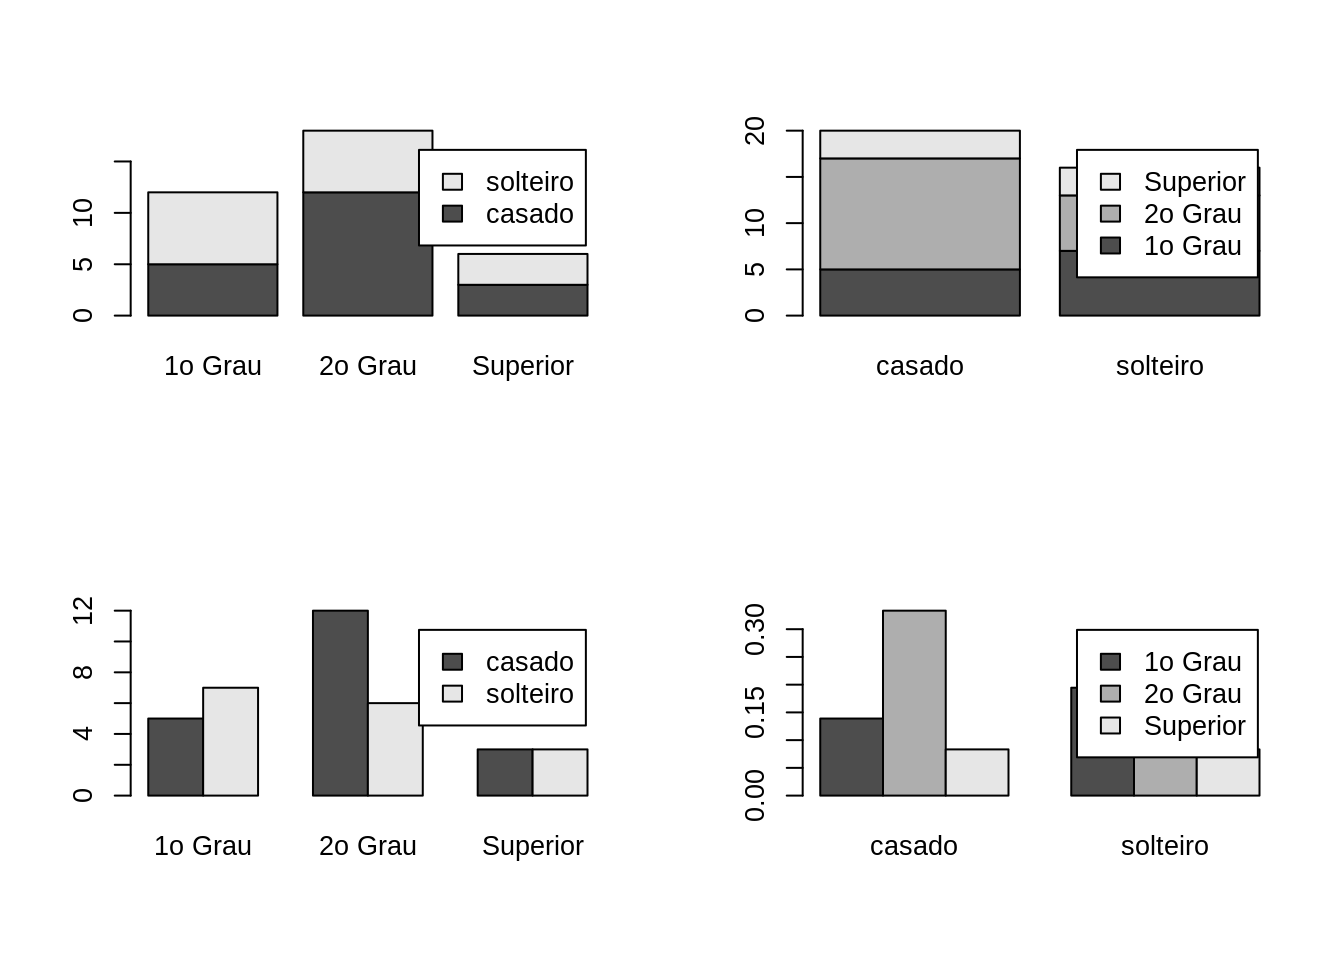
\includegraphics{figures/unnamed-chunk-317-1} \end{center}

\hypertarget{qualitativa-vs-quantitativa}{%
\subsection{\texorpdfstring{Qualitativa \emph{vs} quantitativa}{Qualitativa vs quantitativa}}\label{qualitativa-vs-quantitativa}}

Para exemplificar este caso vamos considerar as variáveis \texttt{Inst} e
\texttt{Salario}.

Para se obter uma tabela de frequências é necessário agrupar a variável
quantitativa em classes. No exemplo a seguir vamos agrupar a variável
salário em 4 classes definidas pelos quartis usando a função \texttt{cut()}.
Lembre-se que as classes são definidas por intervalos abertos à esquerda,
então usamos o argumento \texttt{include.lowest\ =\ TRUE} para garantir que todos
os dados, inclusive o menor (mínimo) seja incluído na primeira classe.
Após agrupar esta variável, obtemos a(s) tabela(s) de cruzamento como
mostrado no caso anterior.

\begin{Shaded}
\begin{Highlighting}[]
\DocumentationTok{\#\# Quartis de salario}
\FunctionTok{quantile}\NormalTok{(milsa}\SpecialCharTok{$}\NormalTok{Salario)}
     \DecValTok{0}\SpecialCharTok{\%     25\%}     \DecValTok{50}\SpecialCharTok{\%     75\%}    \DecValTok{100}\NormalTok{\% }
 \FloatTok{4.0000}  \FloatTok{7.5525} \FloatTok{10.1650} \FloatTok{14.0600} \FloatTok{23.3000} 
\DocumentationTok{\#\# Classificação de acordo com os quartis}
\NormalTok{salario.cut }\OtherTok{\textless{}{-}} \FunctionTok{cut}\NormalTok{(milsa}\SpecialCharTok{$}\NormalTok{Salario, }\AttributeTok{breaks =}  \FunctionTok{quantile}\NormalTok{(milsa}\SpecialCharTok{$}\NormalTok{Salario),}
                   \AttributeTok{include.lowest =} \ConstantTok{TRUE}\NormalTok{)}
\DocumentationTok{\#\# Tabela de frequências absolutas}
\NormalTok{inst.sal.tb }\OtherTok{\textless{}{-}} \FunctionTok{table}\NormalTok{(milsa}\SpecialCharTok{$}\NormalTok{Inst, salario.cut)}
\NormalTok{inst.sal.tb}
\NormalTok{          salario.cut}
\NormalTok{           [}\DecValTok{4}\NormalTok{,}\FloatTok{7.55}\NormalTok{] (}\FloatTok{7.55}\NormalTok{,}\FloatTok{10.2}\NormalTok{] (}\FloatTok{10.2}\NormalTok{,}\FloatTok{14.1}\NormalTok{] (}\FloatTok{14.1}\NormalTok{,}\FloatTok{23.3}\NormalTok{]}
\NormalTok{  1o Grau         }\DecValTok{7}           \DecValTok{3}           \DecValTok{2}           \DecValTok{0}
\NormalTok{  2o Grau         }\DecValTok{2}           \DecValTok{6}           \DecValTok{5}           \DecValTok{5}
\NormalTok{  Superior        }\DecValTok{0}           \DecValTok{0}           \DecValTok{2}           \DecValTok{4}
\FunctionTok{prop.table}\NormalTok{(inst.sal.tb, }\AttributeTok{margin =} \DecValTok{1}\NormalTok{)}
\NormalTok{          salario.cut}
\NormalTok{            [}\DecValTok{4}\NormalTok{,}\FloatTok{7.55}\NormalTok{] (}\FloatTok{7.55}\NormalTok{,}\FloatTok{10.2}\NormalTok{] (}\FloatTok{10.2}\NormalTok{,}\FloatTok{14.1}\NormalTok{] (}\FloatTok{14.1}\NormalTok{,}\FloatTok{23.3}\NormalTok{]}
\NormalTok{  1o Grau  }\FloatTok{0.5833333}   \FloatTok{0.2500000}   \FloatTok{0.1666667}   \FloatTok{0.0000000}
\NormalTok{  2o Grau  }\FloatTok{0.1111111}   \FloatTok{0.3333333}   \FloatTok{0.2777778}   \FloatTok{0.2777778}
\NormalTok{  Superior }\FloatTok{0.0000000}   \FloatTok{0.0000000}   \FloatTok{0.3333333}   \FloatTok{0.6666667}
\end{Highlighting}
\end{Shaded}

No gráfico vamos considerar que neste exemplo a instrução deve ser a
variável explicativa e portanto colocada no eixo X, e o salário é a
variável resposta, e portanto deve ser colocada no eixo Y. Isto é,
consideramos que a instrução deve explicar, ainda que parcialmente, o
salário (e não o contrário!).

Vamos então obter um \emph{boxplot} dos salários para cada nível de
instrução. Note que na função abaixo, usamos a notação de \textbf{fórmula} do
R, com \texttt{Salario\ \textasciitilde{}\ Inst} indicando que a variável \texttt{Salario} é explicada,
ou descrita, (\(\sim\)) pela variável \texttt{Inst}.

\begin{Shaded}
\begin{Highlighting}[]
\FunctionTok{boxplot}\NormalTok{(Salario }\SpecialCharTok{\textasciitilde{}}\NormalTok{ Inst, }\AttributeTok{data =}\NormalTok{ milsa)}
\end{Highlighting}
\end{Shaded}

\begin{center}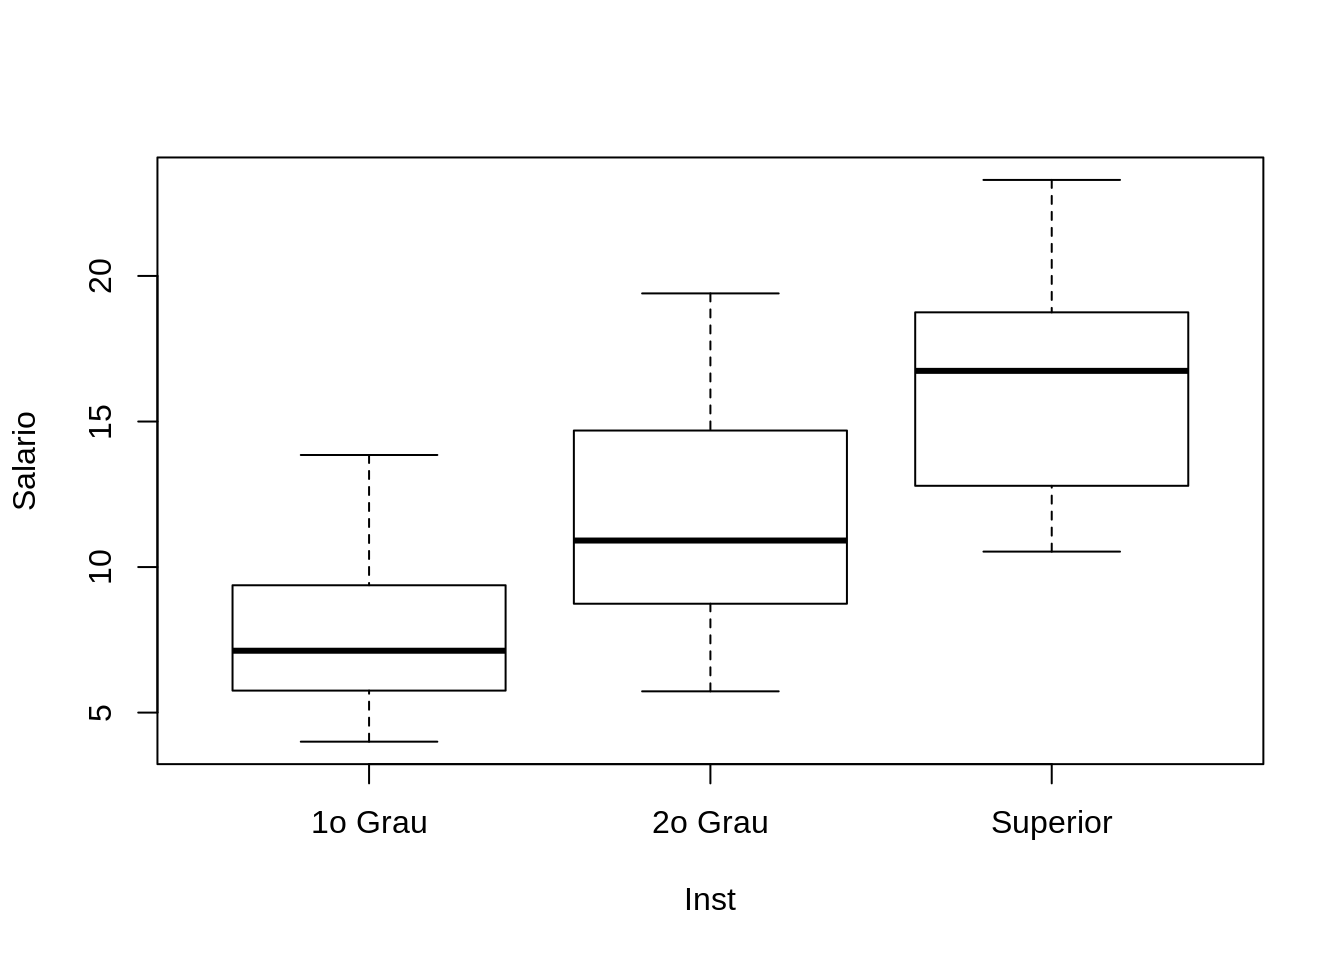
\includegraphics{figures/unnamed-chunk-319-1} \end{center}

Poderíamos ainda fazer gráficos com a variável \texttt{Salario} agrupada
em classes, e neste caso os gráficos seriam como no caso anterior com
duas variáveis qualitativas.

Para as medidas descritivas, o usual é obter um resumo da variável
quantitativa como mostrado na análise univariada, porém agora informando
este resumo para cada nível do fator qualitativo de interesse.

A seguir mostramos alguns exemplos de como obter a média, desvio
padrão e o resumo de cinco números do salário para cada nível de
instrução.

\begin{Shaded}
\begin{Highlighting}[]
\FunctionTok{with}\NormalTok{(milsa, }\FunctionTok{tapply}\NormalTok{(Salario, Inst, mean))}
\NormalTok{  1o Grau   2o Grau  Superior }
 \FloatTok{7.836667} \FloatTok{11.528333} \FloatTok{16.475000} 
\FunctionTok{with}\NormalTok{(milsa, }\FunctionTok{tapply}\NormalTok{(Salario, Inst, sd))}
\NormalTok{ 1o Grau  2o Grau Superior }
\FloatTok{2.956464} \FloatTok{3.715144} \FloatTok{4.502438} 
\FunctionTok{with}\NormalTok{(milsa, }\FunctionTok{tapply}\NormalTok{(Salario, Inst, quantile))}
\SpecialCharTok{$}\StringTok{\textasciigrave{}}\AttributeTok{1o Grau}\StringTok{\textasciigrave{}}
     \DecValTok{0}\SpecialCharTok{\%     25\%}     \DecValTok{50}\SpecialCharTok{\%     75\%}    \DecValTok{100}\NormalTok{\% }
 \FloatTok{4.0000}  \FloatTok{6.0075}  \FloatTok{7.1250}  \FloatTok{9.1625} \FloatTok{13.8500} 

\SpecialCharTok{$}\StringTok{\textasciigrave{}}\AttributeTok{2o Grau}\StringTok{\textasciigrave{}}
     \DecValTok{0}\SpecialCharTok{\%     25\%}     \DecValTok{50}\SpecialCharTok{\%     75\%}    \DecValTok{100}\NormalTok{\% }
 \FloatTok{5.7300}  \FloatTok{8.8375} \FloatTok{10.9100} \FloatTok{14.4175} \FloatTok{19.4000} 

\SpecialCharTok{$}\NormalTok{Superior}
     \DecValTok{0}\SpecialCharTok{\%     25\%}     \DecValTok{50}\SpecialCharTok{\%     75\%}    \DecValTok{100}\NormalTok{\% }
\FloatTok{10.5300} \FloatTok{13.6475} \FloatTok{16.7400} \FloatTok{18.3775} \FloatTok{23.3000} 
\end{Highlighting}
\end{Shaded}

\begin{quote}
NOTE que aqui usamos a função \texttt{tapply()}. Para saber mais sobre os
recursos dessa função e de outras da família \texttt{*apply}, veja o
\href{scripts/script_gapminder.R}{script\_gapminder.R}.
\end{quote}

\hypertarget{quantitativa-vs-quantitativa}{%
\subsection{\texorpdfstring{Quantitativa \emph{vs} Quantitativa}{Quantitativa vs Quantitativa}}\label{quantitativa-vs-quantitativa}}

Para ilustrar este caso vamos considerar as variáveis \texttt{Salario} e
\texttt{Idade}. Para se obter uma tabela é necessário agrupar as
variáveis em classes conforme fizemos no caso anterior.

Nos comandos abaixo, agrupamos as duas variáveis em classes definidas
pelos respectivos quartis, gerando portanto uma tabela de cruzamento
\(4~\times~4\).

\begin{Shaded}
\begin{Highlighting}[]
\DocumentationTok{\#\# Classes de Idade}
\NormalTok{idade.cut }\OtherTok{\textless{}{-}} \FunctionTok{with}\NormalTok{(milsa, }\FunctionTok{cut}\NormalTok{(Idade, }\AttributeTok{breaks =} \FunctionTok{quantile}\NormalTok{(Idade),}
                             \AttributeTok{include.lowest =} \ConstantTok{TRUE}\NormalTok{))}
\FunctionTok{table}\NormalTok{(idade.cut)}
\NormalTok{idade.cut}
\NormalTok{[}\FloatTok{20.8}\NormalTok{,}\FloatTok{30.7}\NormalTok{] (}\FloatTok{30.7}\NormalTok{,}\FloatTok{34.9}\NormalTok{] (}\FloatTok{34.9}\NormalTok{,}\FloatTok{40.5}\NormalTok{] (}\FloatTok{40.5}\NormalTok{,}\FloatTok{48.9}\NormalTok{] }
          \DecValTok{9}           \DecValTok{9}           \DecValTok{9}           \DecValTok{9} 
\DocumentationTok{\#\# Classes de salario}
\NormalTok{salario.cut }\OtherTok{\textless{}{-}} \FunctionTok{with}\NormalTok{(milsa, }\FunctionTok{cut}\NormalTok{(Salario, }\AttributeTok{breaks =} \FunctionTok{quantile}\NormalTok{(Salario),}
                               \AttributeTok{include.lowest =} \ConstantTok{TRUE}\NormalTok{))}
\FunctionTok{table}\NormalTok{(salario.cut)}
\NormalTok{salario.cut}
\NormalTok{   [}\DecValTok{4}\NormalTok{,}\FloatTok{7.55}\NormalTok{] (}\FloatTok{7.55}\NormalTok{,}\FloatTok{10.2}\NormalTok{] (}\FloatTok{10.2}\NormalTok{,}\FloatTok{14.1}\NormalTok{] (}\FloatTok{14.1}\NormalTok{,}\FloatTok{23.3}\NormalTok{] }
          \DecValTok{9}           \DecValTok{9}           \DecValTok{9}           \DecValTok{9} 
\DocumentationTok{\#\# Tabela cruzada}
\FunctionTok{table}\NormalTok{(idade.cut, salario.cut)}
\NormalTok{             salario.cut}
\NormalTok{idade.cut     [}\DecValTok{4}\NormalTok{,}\FloatTok{7.55}\NormalTok{] (}\FloatTok{7.55}\NormalTok{,}\FloatTok{10.2}\NormalTok{] (}\FloatTok{10.2}\NormalTok{,}\FloatTok{14.1}\NormalTok{] (}\FloatTok{14.1}\NormalTok{,}\FloatTok{23.3}\NormalTok{]}
\NormalTok{  [}\FloatTok{20.8}\NormalTok{,}\FloatTok{30.7}\NormalTok{]        }\DecValTok{4}           \DecValTok{2}           \DecValTok{2}           \DecValTok{1}
\NormalTok{  (}\FloatTok{30.7}\NormalTok{,}\FloatTok{34.9}\NormalTok{]        }\DecValTok{1}           \DecValTok{3}           \DecValTok{3}           \DecValTok{2}
\NormalTok{  (}\FloatTok{34.9}\NormalTok{,}\FloatTok{40.5}\NormalTok{]        }\DecValTok{1}           \DecValTok{3}           \DecValTok{2}           \DecValTok{3}
\NormalTok{  (}\FloatTok{40.5}\NormalTok{,}\FloatTok{48.9}\NormalTok{]        }\DecValTok{3}           \DecValTok{1}           \DecValTok{2}           \DecValTok{3}
\FunctionTok{prop.table}\NormalTok{(}\FunctionTok{table}\NormalTok{(idade.cut, salario.cut), }\AttributeTok{margin =} \DecValTok{1}\NormalTok{)}
\NormalTok{             salario.cut}
\NormalTok{idade.cut      [}\DecValTok{4}\NormalTok{,}\FloatTok{7.55}\NormalTok{] (}\FloatTok{7.55}\NormalTok{,}\FloatTok{10.2}\NormalTok{] (}\FloatTok{10.2}\NormalTok{,}\FloatTok{14.1}\NormalTok{] (}\FloatTok{14.1}\NormalTok{,}\FloatTok{23.3}\NormalTok{]}
\NormalTok{  [}\FloatTok{20.8}\NormalTok{,}\FloatTok{30.7}\NormalTok{] }\FloatTok{0.4444444}   \FloatTok{0.2222222}   \FloatTok{0.2222222}   \FloatTok{0.1111111}
\NormalTok{  (}\FloatTok{30.7}\NormalTok{,}\FloatTok{34.9}\NormalTok{] }\FloatTok{0.1111111}   \FloatTok{0.3333333}   \FloatTok{0.3333333}   \FloatTok{0.2222222}
\NormalTok{  (}\FloatTok{34.9}\NormalTok{,}\FloatTok{40.5}\NormalTok{] }\FloatTok{0.1111111}   \FloatTok{0.3333333}   \FloatTok{0.2222222}   \FloatTok{0.3333333}
\NormalTok{  (}\FloatTok{40.5}\NormalTok{,}\FloatTok{48.9}\NormalTok{] }\FloatTok{0.3333333}   \FloatTok{0.1111111}   \FloatTok{0.2222222}   \FloatTok{0.3333333}
\end{Highlighting}
\end{Shaded}

Caso queiramos definir um número menor de classes podemos fazer como no
exemplo a seguir onde cada variável é dividida em 3 classes e gerando um
tabela de cruzamento \(3~\times~3\).

\begin{Shaded}
\begin{Highlighting}[]
\NormalTok{idade.cut2 }\OtherTok{\textless{}{-}} \FunctionTok{with}\NormalTok{(milsa, }\FunctionTok{cut}\NormalTok{(Idade,}
                              \AttributeTok{breaks =} \FunctionTok{quantile}\NormalTok{(Idade, }\FunctionTok{seq}\NormalTok{(}\DecValTok{0}\NormalTok{, }\DecValTok{1}\NormalTok{, }\AttributeTok{length =} \DecValTok{4}\NormalTok{)),}
                              \AttributeTok{include.lowest =} \ConstantTok{TRUE}\NormalTok{))}
\NormalTok{salario.cut2 }\OtherTok{\textless{}{-}} \FunctionTok{with}\NormalTok{(milsa, }\FunctionTok{cut}\NormalTok{(Salario,}
                                \AttributeTok{breaks =} \FunctionTok{quantile}\NormalTok{(Salario, }\FunctionTok{seq}\NormalTok{(}\DecValTok{0}\NormalTok{, }\DecValTok{1}\NormalTok{, }\AttributeTok{length =} \DecValTok{4}\NormalTok{)),}
                                \AttributeTok{include.lowest =} \ConstantTok{TRUE}\NormalTok{))}
\FunctionTok{table}\NormalTok{(idade.cut2, salario.cut2)}
\NormalTok{             salario.cut2}
\NormalTok{idade.cut2    [}\DecValTok{4}\NormalTok{,}\FloatTok{8.65}\NormalTok{] (}\FloatTok{8.65}\NormalTok{,}\FloatTok{12.9}\NormalTok{] (}\FloatTok{12.9}\NormalTok{,}\FloatTok{23.3}\NormalTok{]}
\NormalTok{  [}\FloatTok{20.8}\NormalTok{,}\FloatTok{32.1}\NormalTok{]        }\DecValTok{5}           \DecValTok{5}           \DecValTok{2}
\NormalTok{  (}\FloatTok{32.1}\NormalTok{,}\FloatTok{37.8}\NormalTok{]        }\DecValTok{4}           \DecValTok{3}           \DecValTok{5}
\NormalTok{  (}\FloatTok{37.8}\NormalTok{,}\FloatTok{48.9}\NormalTok{]        }\DecValTok{3}           \DecValTok{4}           \DecValTok{5}
\FunctionTok{prop.table}\NormalTok{(}\FunctionTok{table}\NormalTok{(idade.cut2, salario.cut2), }\AttributeTok{margin =} \DecValTok{1}\NormalTok{)}
\NormalTok{             salario.cut2}
\NormalTok{idade.cut2     [}\DecValTok{4}\NormalTok{,}\FloatTok{8.65}\NormalTok{] (}\FloatTok{8.65}\NormalTok{,}\FloatTok{12.9}\NormalTok{] (}\FloatTok{12.9}\NormalTok{,}\FloatTok{23.3}\NormalTok{]}
\NormalTok{  [}\FloatTok{20.8}\NormalTok{,}\FloatTok{32.1}\NormalTok{] }\FloatTok{0.4166667}   \FloatTok{0.4166667}   \FloatTok{0.1666667}
\NormalTok{  (}\FloatTok{32.1}\NormalTok{,}\FloatTok{37.8}\NormalTok{] }\FloatTok{0.3333333}   \FloatTok{0.2500000}   \FloatTok{0.4166667}
\NormalTok{  (}\FloatTok{37.8}\NormalTok{,}\FloatTok{48.9}\NormalTok{] }\FloatTok{0.2500000}   \FloatTok{0.3333333}   \FloatTok{0.4166667}
\end{Highlighting}
\end{Shaded}

O gráfico adequado para representar duas variáveis quantitativas é
um diagrama de dispersão. Note que se as variáveis envolvidas puderem
ser classificadas como ``explicativa'' e ``resposta'' devemos colocar a
primeira no eixo X e a segunda no eixo Y. Neste exemplo é razoável
admitir que a idade deve explicar, ao menos parcialmente, o salário e
portanto fazemos o gráfico com idade no eixo X. Note que na função
\texttt{plot()}, podemos usar tanto os argumentos \texttt{x} e \texttt{y}, quanto o formato
de fórmula (como visto anteriormente).

\begin{Shaded}
\begin{Highlighting}[]
\FunctionTok{plot}\NormalTok{(}\AttributeTok{x =}\NormalTok{ milsa}\SpecialCharTok{$}\NormalTok{Idade, }\AttributeTok{y =}\NormalTok{ milsa}\SpecialCharTok{$}\NormalTok{Salario)}
\FunctionTok{plot}\NormalTok{(Salario }\SpecialCharTok{\textasciitilde{}}\NormalTok{ Idade, }\AttributeTok{data =}\NormalTok{ milsa)}
\end{Highlighting}
\end{Shaded}

\begin{center}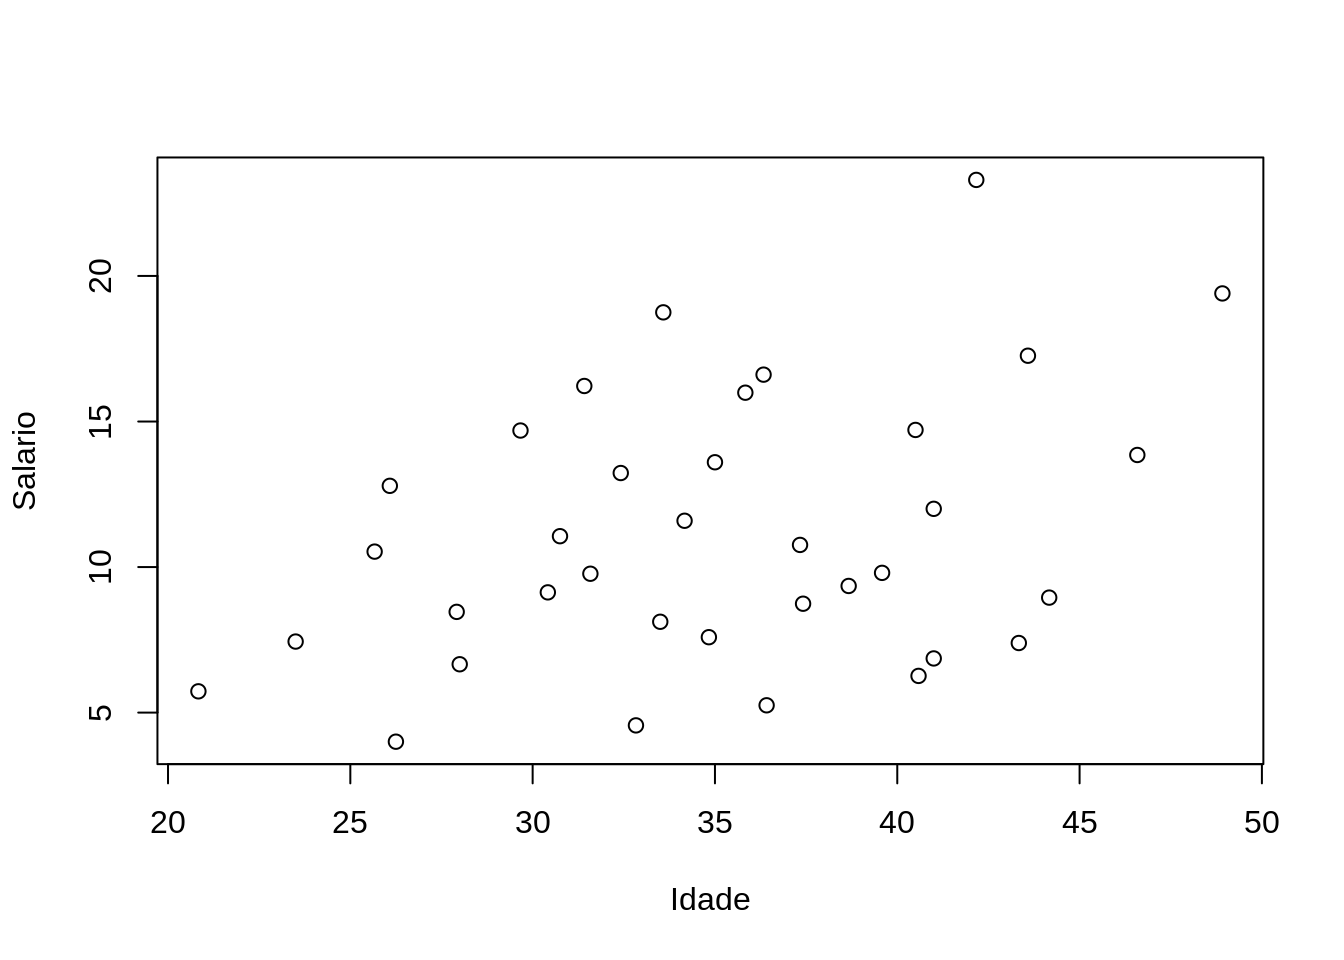
\includegraphics{figures/unnamed-chunk-323-1} \end{center}

Para quantificar a associação entre variáveis deste tipo, usamos o
coeficiente de correlação. A função \texttt{cor()} possui opção para três
coeficientes de correlação, tendo como \emph{default} o coeficiente de
correlação linear de Pearson.

\begin{Shaded}
\begin{Highlighting}[]
\FunctionTok{with}\NormalTok{(milsa, }\FunctionTok{cor}\NormalTok{(Idade, Salario))}
\NormalTok{[}\DecValTok{1}\NormalTok{] }\FloatTok{0.3651397}
\FunctionTok{with}\NormalTok{(milsa, }\FunctionTok{cor}\NormalTok{(Idade, Salario, }\AttributeTok{method =} \StringTok{"kendall"}\NormalTok{))}
\NormalTok{[}\DecValTok{1}\NormalTok{] }\FloatTok{0.214456}
\FunctionTok{with}\NormalTok{(milsa, }\FunctionTok{cor}\NormalTok{(Idade, Salario, }\AttributeTok{method =} \StringTok{"spearman"}\NormalTok{))}
\NormalTok{[}\DecValTok{1}\NormalTok{] }\FloatTok{0.2895939}
\end{Highlighting}
\end{Shaded}

\hypertarget{exercuxedcios-15}{%
\section*{Exercícios}\label{exercuxedcios-15}}


\begin{enumerate}
\def\labelenumi{\arabic{enumi}.}
\item
  Experimente as funções \texttt{mean()}, \texttt{var()}, \texttt{sd()}, \texttt{median()},
  \texttt{quantile()} nos dados mostrados anteriormente (\texttt{milsa}). Veja a
  documentação das funções e as opções de uso.
\item
  Carregue o conjunto de dados \texttt{women} com \texttt{data(women)}. Veja o que
  são os dados com \texttt{help(women)}, e faça uma análise descritiva
  adequada.
\item
  Carregue o conjunto de dados \texttt{USArrests} com
  \texttt{data(USArrests)}. Examine a sua documentação com \texttt{help(USArrests)} e
  responda as perguntas a seguir:

  \begin{enumerate}
  \def\labelenumii{\arabic{enumii}.}
  \tightlist
  \item
    Qual o número médio e mediano de cada um dos crimes?
  \item
    Encontre a mediana e quartis para cada crime.
  \item
    Encontre o número máximo e mínimo para cada crime.
  \item
    Faça um gráfico adequado para o número de assassinatos (\texttt{Murder}).
  \item
    Faça um \emph{boxplot} para o número de estupros (\texttt{Rape}).
  \item
    Verifique se há correlação entre os diferentes tipos de crime.
  \item
    Verifique se há correlação entre os crimes e a proporção de
    população urbana.
  \item
    Encontre os estados com maior e menor ocorrência de cada tipo de
    crime.
  \item
    Encontre os estados com maior e menor ocorrência per capta de cada
    tipo de crime.
  \item
    Encontre os estados com maior e menor ocorrência do total de
    crimes.
  \item
    Calcule a média de crimes (entre \texttt{Murder}, \texttt{Assault} e \texttt{Rape})
    para cada estado.
  \end{enumerate}
\end{enumerate}

A resolução de todos os exercícios desta página está disponível neste
\href{scripts/analise-exploratoria-exercicios.R}{script}.

\hypertarget{probabilidade-e-variuxe1veis-aleatuxf3rias}{%
\chapter{Probabilidade e variáveis aleatórias}\label{probabilidade-e-variuxe1veis-aleatuxf3rias}}

\hypertarget{conceitos-buxe1sicos-sobre-distribuiuxe7uxf5es-de-probabilidade}{%
\section{Conceitos básicos sobre distribuições de probabilidade}\label{conceitos-buxe1sicos-sobre-distribuiuxe7uxf5es-de-probabilidade}}

O objetivo desta sessão é mostrar o uso de funções do R em problemas de
probabilidade. Exercícios que podem (e devem!) ser resolvidos
analiticamente, serão utilizados para ilustrar o uso do programa e
alguns de seus recursos para análises numéricas.

Os problemas desta sessão foram retirados do livro de \href{https://www.ime.usp.br/~pam/EstBas.html}{Bussab e Morettin
(2017)}. Veja também os códigos
do R dos exemplos do livro para os capítulos 6 e 7, disponíveis
\href{https://rpubs.com/EstatBasica/Introd}{aqui}.

\textbf{Exemplo 1}: (Adaptado de Bussab e Morettin, cap. 7 ex. 1)

Dada a função

\[
\
  f(x) = \left\{ \begin{array}{ll}
      2 e^{-2x} & \mbox{ , se $ \; x \geq 0$} \cr
      0   & \mbox{ , se  $ \; x < 0$}
    \end{array} \right.
\
\]

\begin{enumerate}
\def\labelenumi{\alph{enumi}.}
\tightlist
\item
  Mostre que está função é uma f.d.p.
\item
  Calcule a probabilidade de que \(X > 1\).
\item
  calcule a probabilidade de que \(0.2 < X < 0.8\).
\end{enumerate}

Para ser f.d.p. a função não deve ter valores negativos e deve integrar
1 em seu domínio. Vamos começar definindo esta função como uma \emph{função}
no R para qual daremos o nome de \texttt{f1}.

\begin{Shaded}
\begin{Highlighting}[]
\NormalTok{f1 }\OtherTok{\textless{}{-}} \ControlFlowTok{function}\NormalTok{(x)\{}
\NormalTok{    fx }\OtherTok{\textless{}{-}} \FunctionTok{ifelse}\NormalTok{(x }\SpecialCharTok{\textless{}} \DecValTok{0}\NormalTok{, }\DecValTok{0}\NormalTok{, }\DecValTok{2} \SpecialCharTok{*} \FunctionTok{exp}\NormalTok{(}\SpecialCharTok{{-}}\DecValTok{2} \SpecialCharTok{*}\NormalTok{ x))}
    \FunctionTok{return}\NormalTok{(fx)}
\NormalTok{\}}
\end{Highlighting}
\end{Shaded}

A seguir fazemos o gráfico da função. Como a função tem valores
positivos para \(x\) no intervalo de zero a infinito, temos que definir
um limite em \(x\) até onde vai o gráfico da função. Vamos achar este
limite tentando vários valores, conforme mostrado nos comandos abaixo.

\begin{Shaded}
\begin{Highlighting}[]
\FunctionTok{par}\NormalTok{(}\AttributeTok{mfrow =} \FunctionTok{c}\NormalTok{(}\DecValTok{2}\NormalTok{, }\DecValTok{2}\NormalTok{))}
\FunctionTok{plot}\NormalTok{(f1)}
\FunctionTok{plot}\NormalTok{(f1, }\AttributeTok{from =} \DecValTok{0}\NormalTok{, }\AttributeTok{to =} \DecValTok{5}\NormalTok{)}
\FunctionTok{plot}\NormalTok{(f1, }\AttributeTok{from =} \DecValTok{0}\NormalTok{, }\AttributeTok{to =} \DecValTok{7}\NormalTok{)}
\FunctionTok{plot}\NormalTok{(f1, }\AttributeTok{from =} \DecValTok{0}\NormalTok{, }\AttributeTok{to =} \DecValTok{10}\NormalTok{)}
\FunctionTok{par}\NormalTok{(}\AttributeTok{mfrow =} \FunctionTok{c}\NormalTok{(}\DecValTok{1}\NormalTok{, }\DecValTok{1}\NormalTok{))}
\end{Highlighting}
\end{Shaded}

\begin{center}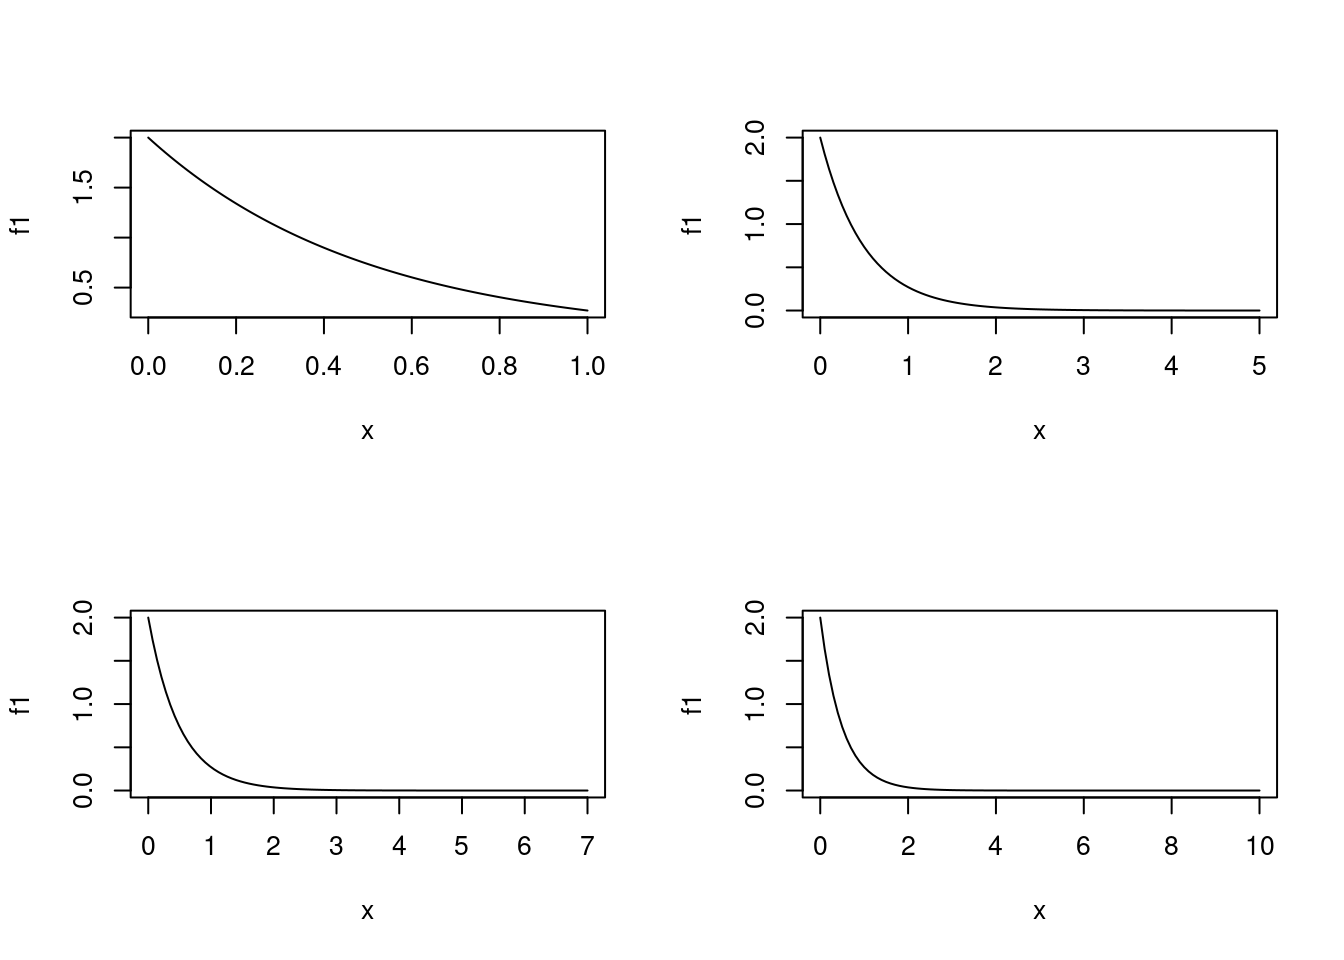
\includegraphics{figures/unnamed-chunk-327-1} \end{center}

Para verificar que a integral da função é igual a 1 podemos usar a
função \texttt{integrate()}, que efetua integração numérica. A função recebe
como argumentos o objeto com a função a ser integrada e os limites de
integração. Neste exemplo o objeto é \texttt{f1} definido acima, e o domínio da
função é \([0, \infty)\). A saída da função mostra o valor da integral
acima, e o erro máximo da aproximação numérica.

\begin{Shaded}
\begin{Highlighting}[]
\FunctionTok{integrate}\NormalTok{(f1, }\AttributeTok{lower =} \DecValTok{0}\NormalTok{, }\AttributeTok{upper =} \ConstantTok{Inf}\NormalTok{)}
\DecValTok{1}\NormalTok{ with absolute error }\SpecialCharTok{\textless{}} \FloatTok{5e{-}07}
\end{Highlighting}
\end{Shaded}

Para fazer os cálculos pedidos nos itens (b) e (c) lembramos que a
probabilidade é dada pela área sob a curva da função no intervalo
pedido. Desta forma as soluções seriam dadas pelas expressões

\begin{eqnarray*}
 p_b & = & P(X > 1) = \int_1^\infty f(x) dx = \int_1^\infty 2\,e^{-2x} dx \\
 p_c & = & P(0,2 < X < 0,8) = \int_{0,2}^{0,8} f(x) dx = \int_{0.2}^{0.8} 2\,e^{-2x} dx \,
\end{eqnarray*}

cuja representação gráfica é mostrada na abaixo.

Os comandos a seguir mostram como fazer o gráfico dessas funções. O
comando \texttt{plot()} desenha o gráfico principal, e para destacar as
áreas que correspondem às probabilidades pedidas vamos usar a função
\texttt{polygon()}. Esta função adiciona a um gráfico um polígono que é
definido pelas coordenadas de seus vértices. Para sombrear a área usa-se
o argumento \texttt{density}. Finalmente, para escrever um texto no gráfico
usamos a função \texttt{text()} com as coordenadas de posição do texto.

\begin{Shaded}
\begin{Highlighting}[]
\FunctionTok{plot}\NormalTok{(f1, }\AttributeTok{from =} \DecValTok{0}\NormalTok{, }\AttributeTok{to =} \DecValTok{5}\NormalTok{)}
\FunctionTok{polygon}\NormalTok{(}\AttributeTok{x =} \FunctionTok{c}\NormalTok{(}\DecValTok{1}\NormalTok{, }\FunctionTok{seq}\NormalTok{(}\DecValTok{1}\NormalTok{, }\DecValTok{5}\NormalTok{, }\AttributeTok{length.out =} \DecValTok{20}\NormalTok{)),}
        \AttributeTok{y =} \FunctionTok{c}\NormalTok{(}\DecValTok{0}\NormalTok{, }\FunctionTok{f1}\NormalTok{(}\FunctionTok{seq}\NormalTok{(}\DecValTok{1}\NormalTok{, }\DecValTok{5}\NormalTok{,}\AttributeTok{length.out =} \DecValTok{20}\NormalTok{))),}
        \AttributeTok{density =} \DecValTok{10}\NormalTok{)}
\FunctionTok{polygon}\NormalTok{(}\AttributeTok{x =} \FunctionTok{c}\NormalTok{(}\FloatTok{0.2}\NormalTok{, }\FunctionTok{seq}\NormalTok{(}\FloatTok{0.2}\NormalTok{, }\FloatTok{0.8}\NormalTok{, }\AttributeTok{length.out =} \DecValTok{20}\NormalTok{), }\FloatTok{0.8}\NormalTok{),}
        \AttributeTok{y =} \FunctionTok{c}\NormalTok{(}\DecValTok{0}\NormalTok{, }\FunctionTok{f1}\NormalTok{(}\FunctionTok{seq}\NormalTok{(}\FloatTok{0.2}\NormalTok{, }\FloatTok{0.8}\NormalTok{, }\AttributeTok{length.out =} \DecValTok{20}\NormalTok{)), }\DecValTok{0}\NormalTok{),}
        \AttributeTok{col =} \StringTok{"gray"}\NormalTok{)}
\FunctionTok{text}\NormalTok{(}\AttributeTok{x =} \FunctionTok{c}\NormalTok{(}\FloatTok{1.2}\NormalTok{, }\FloatTok{0.5}\NormalTok{), }\AttributeTok{y =} \FunctionTok{c}\NormalTok{(}\FloatTok{0.1}\NormalTok{, }\FloatTok{0.2}\NormalTok{),}
     \FunctionTok{c}\NormalTok{(}\FunctionTok{expression}\NormalTok{(p[b], p[c])))}
\end{Highlighting}
\end{Shaded}

\begin{center}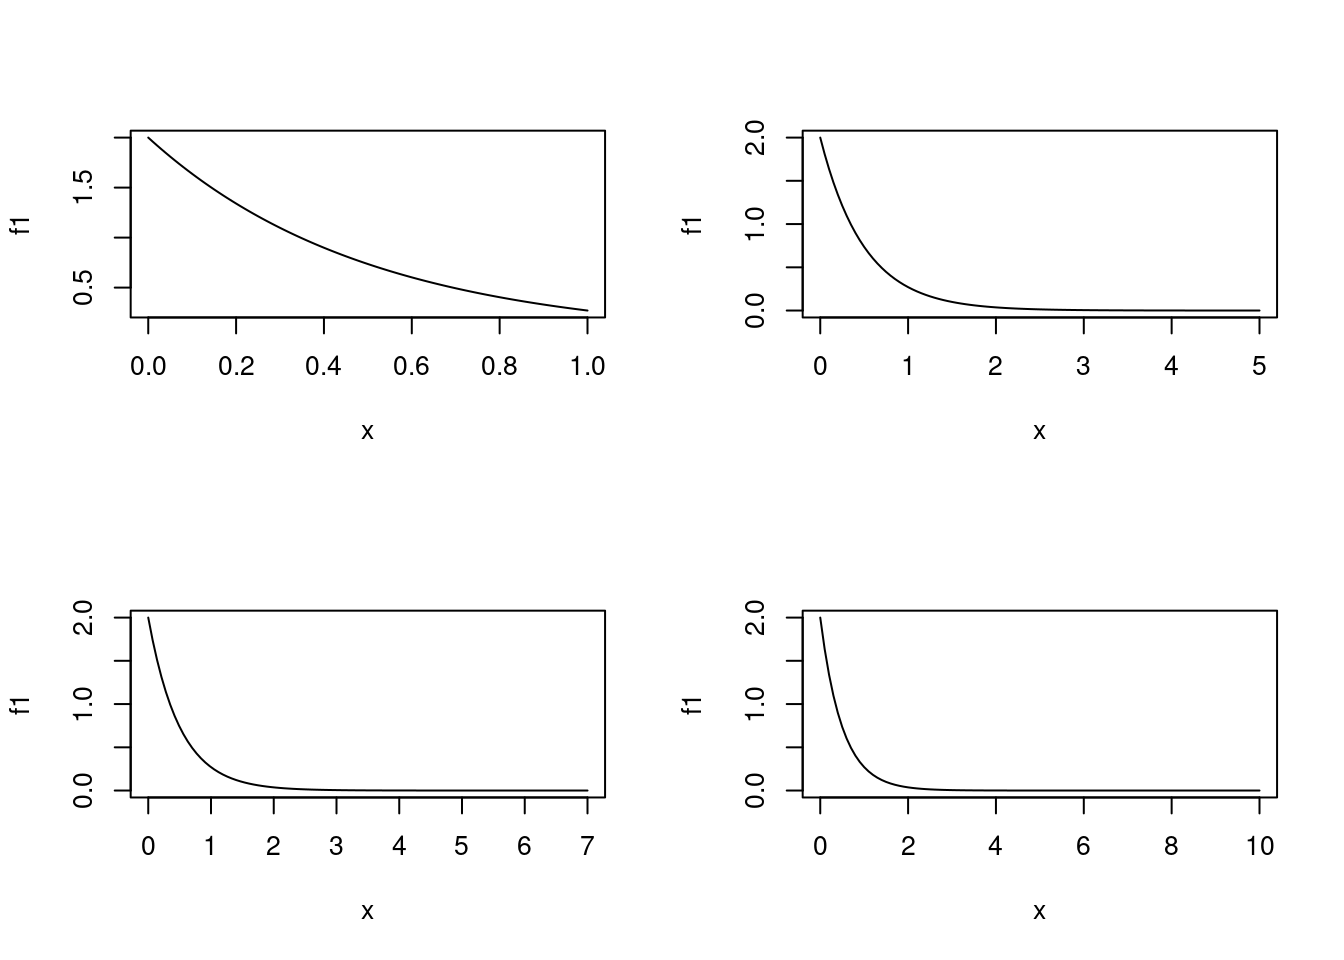
\includegraphics{figures/unnamed-chunk-329-1} \end{center}

Oara obter as probabilidades pedidas usamos a função \texttt{integrate()}.

\begin{Shaded}
\begin{Highlighting}[]
\FunctionTok{integrate}\NormalTok{(f1, }\AttributeTok{lower =} \DecValTok{1}\NormalTok{, }\AttributeTok{upper =} \ConstantTok{Inf}\NormalTok{)}
\FloatTok{0.1353353}\NormalTok{ with absolute error }\SpecialCharTok{\textless{}} \FloatTok{2.1e{-}05}
\FunctionTok{integrate}\NormalTok{(f1, }\AttributeTok{lower =} \FloatTok{0.2}\NormalTok{, }\AttributeTok{upper =} \FloatTok{0.8}\NormalTok{)}
\FloatTok{0.4684235}\NormalTok{ with absolute error }\SpecialCharTok{\textless{}} \FloatTok{5.2e{-}15}
\end{Highlighting}
\end{Shaded}

\textbf{Exemplo 2}: (Adaptado de Bussab e Morettin, cap. 7 ex. 10)

A demanda diária de arroz em um supermercado, em centenas de quilos, é
uma v.a \(X\) com f.d.p. dada por

\begin{eqnarray}
  f(x) = \left\{ \begin{array}{ll}
      \frac{2}{3}x \mbox{ , se $0 \leq x < 1$} \cr
      -\frac{x}{3} + 1 \mbox{ , se $ 1 \leq x < 3$} \cr
      0            \mbox{ , se $x < 0$  ou  $x \geq 3$}
    \end{array} \right.
\end{eqnarray}

\begin{enumerate}
\def\labelenumi{\alph{enumi}.}
\tightlist
\item
  Calcular a probabilidade de que sejam vendidos mais que 150 kg.
\item
  Calcular a venda esperada em 30 dias.
\end{enumerate}

Novamente começamos definindo um objeto do R que contém a função dada
acima. Neste caso definimos um vetor do mesmo tamanho do argumento \texttt{x}
para armazenar os valores de \(f(x)\) e a seguir preenchemos os valores
deste vetor para cada faixa de valor de \(x\):

\begin{Shaded}
\begin{Highlighting}[]
\NormalTok{f2 }\OtherTok{\textless{}{-}} \ControlFlowTok{function}\NormalTok{(x)\{}
\NormalTok{  fx }\OtherTok{\textless{}{-}} \FunctionTok{numeric}\NormalTok{(}\FunctionTok{length}\NormalTok{(x))}
\NormalTok{  fx[x }\SpecialCharTok{\textless{}} \DecValTok{0}\NormalTok{] }\OtherTok{\textless{}{-}} \DecValTok{0}
\NormalTok{  fx[x }\SpecialCharTok{\textgreater{}=} \DecValTok{0} \SpecialCharTok{\&}\NormalTok{ x }\SpecialCharTok{\textless{}} \DecValTok{1}\NormalTok{] }\OtherTok{\textless{}{-}}\NormalTok{ (}\DecValTok{2}\SpecialCharTok{/}\DecValTok{3}\NormalTok{) }\SpecialCharTok{*}\NormalTok{ x[x }\SpecialCharTok{\textgreater{}=} \DecValTok{0} \SpecialCharTok{\&}\NormalTok{ x }\SpecialCharTok{\textless{}} \DecValTok{1}\NormalTok{]}
\NormalTok{  fx[x }\SpecialCharTok{\textgreater{}=} \DecValTok{1} \SpecialCharTok{\&}\NormalTok{ x }\SpecialCharTok{\textless{}} \DecValTok{3}\NormalTok{] }\OtherTok{\textless{}{-}}\NormalTok{ (}\SpecialCharTok{{-}}\DecValTok{1}\SpecialCharTok{/}\DecValTok{3}\NormalTok{) }\SpecialCharTok{*}\NormalTok{ x[x }\SpecialCharTok{\textgreater{}=} \DecValTok{1} \SpecialCharTok{\&}\NormalTok{ x }\SpecialCharTok{\textless{}} \DecValTok{3}\NormalTok{] }\SpecialCharTok{+} \DecValTok{1}
\NormalTok{  fx[x }\SpecialCharTok{\textgreater{}=} \DecValTok{3}\NormalTok{] }\OtherTok{\textless{}{-}} \DecValTok{0}
  \FunctionTok{return}\NormalTok{(fx)}
\NormalTok{\}}
\end{Highlighting}
\end{Shaded}

A seguir verificamos que a integral da função é 1 e fazemos o seu gráfico
conforme mostrado abaixo:

\begin{Shaded}
\begin{Highlighting}[]
\FunctionTok{integrate}\NormalTok{(f2, }\DecValTok{0}\NormalTok{, }\DecValTok{3}\NormalTok{) }\DocumentationTok{\#\# verificando que a integral vale 1}
\DecValTok{1}\NormalTok{ with absolute error }\SpecialCharTok{\textless{}} \FloatTok{1.1e{-}15}
\FunctionTok{plot}\NormalTok{(f2, }\SpecialCharTok{{-}}\DecValTok{1}\NormalTok{, }\DecValTok{4}\NormalTok{)     }\DocumentationTok{\#\# fazendo o gráfico da função}
\end{Highlighting}
\end{Shaded}

\begin{center}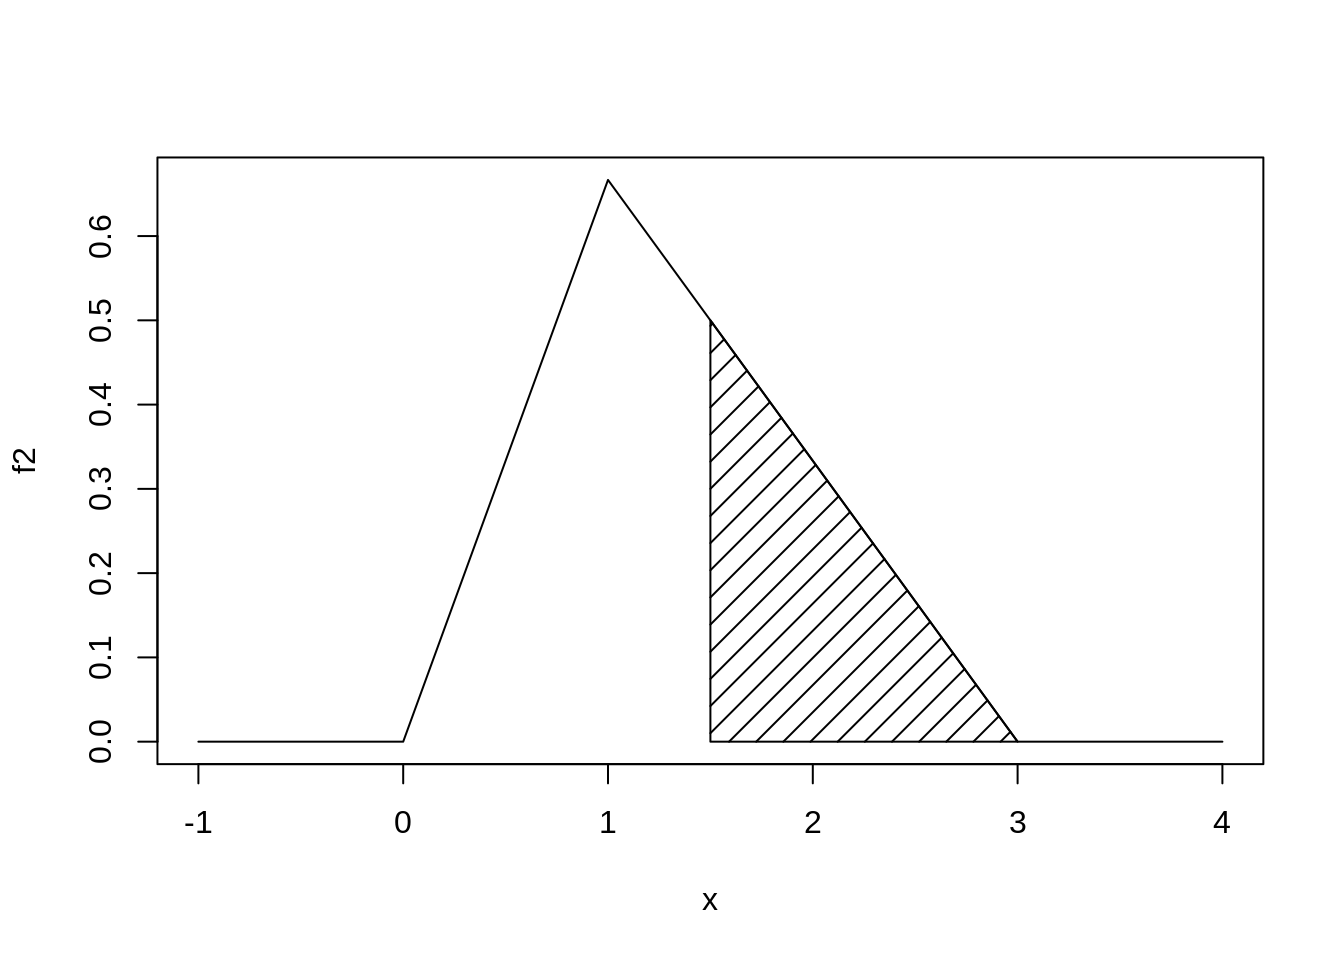
\includegraphics{figures/unnamed-chunk-332-1} \end{center}

Agora vamos responder às questões levantadas. Na questão (a) pede-se a
probabilidade de que sejam vendidos mais que 150 kg (1,5 centenas de
quilos), portanto a probabilidade \(P[X > 1,5]\). A probabilidade
corresponde à área sob a função no intervalo pedido, ou seja,
\(P[X > 1,5] = \int_{1,5}^\infty f(x) dx\), que pode ser vista na figura
abaixo.

\begin{Shaded}
\begin{Highlighting}[]
\FunctionTok{plot}\NormalTok{(f2, }\SpecialCharTok{{-}}\DecValTok{1}\NormalTok{, }\DecValTok{4}\NormalTok{)}
\FunctionTok{polygon}\NormalTok{(}\AttributeTok{x =} \FunctionTok{c}\NormalTok{(}\FloatTok{1.5}\NormalTok{, }\FloatTok{1.5}\NormalTok{, }\DecValTok{3}\NormalTok{), }\AttributeTok{y =} \FunctionTok{c}\NormalTok{(}\DecValTok{0}\NormalTok{, }\FunctionTok{f2}\NormalTok{(}\FloatTok{1.5}\NormalTok{), }\DecValTok{0}\NormalTok{), }\AttributeTok{dens =} \DecValTok{10}\NormalTok{)}
\end{Highlighting}
\end{Shaded}

\begin{center}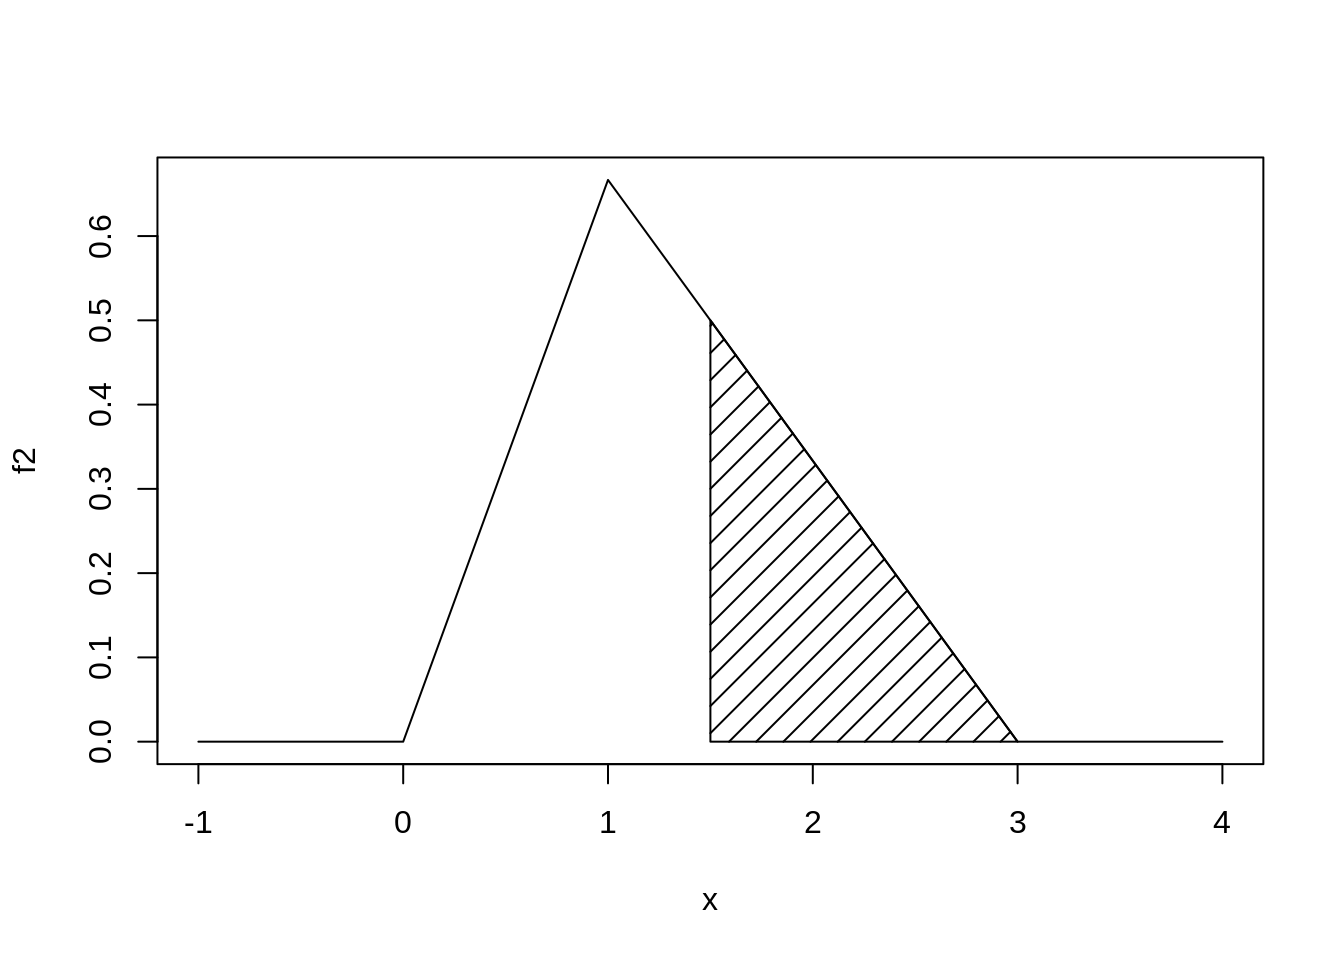
\includegraphics{figures/unnamed-chunk-333-1} \end{center}

A integral pode então ser resolvida numericamente com o comando:

\begin{Shaded}
\begin{Highlighting}[]
\FunctionTok{integrate}\NormalTok{(f2, }\FloatTok{1.5}\NormalTok{, }\DecValTok{3}\NormalTok{)}
\FloatTok{0.375}\NormalTok{ with absolute error }\SpecialCharTok{\textless{}} \FloatTok{4.2e{-}15}
\end{Highlighting}
\end{Shaded}

A venda esperada em trinta dias é 30 vezes o valor esperado de venda em
um dia. Para calcular a esperança \(E[X] = \int x f(x) dx\) definimos uma
nova função e resolvemos a integral. A função \texttt{integrate()} retorna uma
lista onde um dos elementos (\texttt{value}) é o valor da integral.

\begin{Shaded}
\begin{Highlighting}[]
\NormalTok{ef2 }\OtherTok{\textless{}{-}} \ControlFlowTok{function}\NormalTok{(x) \{ x }\SpecialCharTok{*} \FunctionTok{f2}\NormalTok{(x) \}}
\FunctionTok{integrate}\NormalTok{(ef2, }\DecValTok{0}\NormalTok{, }\DecValTok{3}\NormalTok{)}
\FloatTok{1.333333}\NormalTok{ with absolute error }\SpecialCharTok{\textless{}} \FloatTok{7.3e{-}05}
\DecValTok{30} \SpecialCharTok{*} \FunctionTok{integrate}\NormalTok{(ef2, }\DecValTok{0}\NormalTok{, }\DecValTok{3}\NormalTok{)}\SpecialCharTok{$}\NormalTok{value}
\NormalTok{[}\DecValTok{1}\NormalTok{] }\DecValTok{40}
\end{Highlighting}
\end{Shaded}

Finalmente lembramos que os exemplos discutidos aqui são simples e não
requerem soluções numéricas, devendo ser resolvidos analiticamente.
Utilizamos estes exemplos somente para ilustrar a obtenção de soluções
numéricas com o uso do R, que na prática deve ser utilizado em
problemas mais complexos onde soluções analíticas não são triviais ou
mesmo impossíveis.

\hypertarget{exercuxedcios-16}{%
\section*{Exercícios}\label{exercuxedcios-16}}


\begin{enumerate}
\def\labelenumi{\arabic{enumi}.}
\tightlist
\item
  (Adaptado de Bussab e Morettin, cap. 7, ex. 28). Em uma determinada
  localidade a distribuição de renda, em u.m. (unidade monetária) é uma
  variável aleatória \(X\) com função de distribuição de probabilidade:
  \[
  f(x) = \left\{ \begin{array}{ll}
       \frac{1}{10}x + \frac{1}{10} & \mbox{ se $0 \leq x \leq 2$} \cr
       -\frac{3}{40}x + \frac{9}{20} & \mbox{ se $ 2 < x \leq 6$} \cr
       0      &      \mbox{ se $x < 0$  ou  $x > 6$}
     \end{array} \right.
  \]

  \begin{enumerate}
  \def\labelenumii{\alph{enumii}.}
  \tightlist
  \item
    Mostre que \(f(x)\) é uma f.d.p.
  \item
    Qual a renda média nesta localidade?
  \item
    Calcule a probabilidade de encontrar uma pessoa com renda acima
    de 4,5 u.m. e indique o resultado no gráfico da distribuição.
  \end{enumerate}
\item
  Sabe-se que uma variável aleatória contínua \(X\) é equiprovável no intervalo 10 e 20.

  \begin{enumerate}
  \def\labelenumii{\alph{enumii}.}
  \tightlist
  \item
    Apresente o gráfico da função densidade de probabilidade.
  \item
    Calcule \(P(X < 15)\).
  \item
    Calcule \(P(12 \leq X \leq 18)\).
  \item
    Calcule \(E(X)\) e \(V(X)\).
  \end{enumerate}
\item
  Dois jogadores se alternam lançando dois dados equilibrados. O jogador A vence o jogo se ocorrer soma 6, enquanto B vencerá se ocorrer 7. Faça um estudo de simulação para responder as seguintes questões:

  \begin{enumerate}
  \def\labelenumii{\alph{enumii}.}
  \tightlist
  \item
    Se A começa jogando, qual é a sua probabilidade de vitória?
  \item
    Qual é a probabilidade do iniciante, escolhido ao acaso, vencer o jogo?
  \end{enumerate}
\item
  A duração, em anos, de uma certa lâmpada especial é uma variável aleatória contínua com densidade dada por:
  \[
  f(x) = \left\{ \begin{array}{ll}
       2 \exp^{-2x} & x \geq 0 \cr
       0 & x < 0
     \end{array} \right.
  \]

  \begin{enumerate}
  \def\labelenumii{\alph{enumii}.}
  \tightlist
  \item
    Crie uma função para calcular a função de distribuição acumulado de \(X\).
  \item
    Calcule \(P(X > 2)\).
  \item
    Calcule \(P(0.5 < X < 1.2)\).
  \item
    Calcule \(P(X > 3)\).
  \item
    Calcule \(P(X < 3| X > 1)\).
  \end{enumerate}
\item
  (Desafio - Problema da ruína do jogador) Dois jogadores participam de um jogo com uma moeda que tem probabilidade de cara igual a \(p\) e de coroa igual a \(q\), sujeito a \(p+q=1\). O jogador A inicia o jogo com \(i\) fichas e ganha mais uma de B, cada vez que der cara. O jogador B começa com \(N-i\) fichas e, em cada lançamento que resultar coroa, ganha uma ficha de A. Para enfatizar a dependência do número inicial de fichas \(i\), denomine por \(p_{(i)}\) a probabilidade do jogador A ficar com todas as fichas, o que implica na ruína de B. Condicione no resultado do primeiro lançamento da moeda, para estabelecer uma relação de recorrência entre os \(p_{(i)'s}\). Usando \(p_{(0)} = 0\) e \(p_{N} = 1\), mostre via simulação que \(p_{(i)} = \frac{1-(q/p)^i}{1-(q/p)^N}\) para \(p \neq \frac{1}{2}\) e \(p_{(i)} = \frac{i}{N}\) para \(p = \frac{1}{2}\).
\end{enumerate}

\hypertarget{distribuiuxe7uxf5es-de-probabilidade}{%
\section{Distribuições de Probabilidade}\label{distribuiuxe7uxf5es-de-probabilidade}}

O R inclui funcionalidade para operações com distribuições de
probabilidades. Para cada distribuição há 4 operações básicas indicadas
pelas letras:

\begin{itemize}
\tightlist
\item
  \texttt{d} calcula a densidade de probabilidade \(f(x)\) no ponto \(x\).
\item
  \texttt{p} calcula a função de probabilidade acumulada \(F(x)\) no ponto \(x\).
\item
  \texttt{q} calcula o quantil correspondente a uma dada probabilidade.
\item
  \texttt{r} retorna uma amostra aleatória da distribuição.
\end{itemize}

Para usar as funções deve-se combinar uma das letras acima com uma
abreviatura do nome da distribuição. Por exemplo, para calcular
probabilidades usamos: \texttt{pnorm()} para normal, \texttt{pexp()} para exponencial,
\texttt{pbinom()} para binomial, \texttt{ppois()} para Poisson e assim por diante.

Vamos ver com mais detalhes algumas distribuições de probabilidades.

\hypertarget{distribuiuxe7uxe3o-normal}{%
\subsection{Distribuição Normal}\label{distribuiuxe7uxe3o-normal}}

A funcionalidade para distribuição normal é implementada por argumentos
que combinam as letras acima com o termo \texttt{norm}. Vamos ver alguns
exemplos com a distribuição normal padrão. Por \texttt{default} as funções
assumem a distribuição normal padrão \(N(\mu=0, \sigma^2=1)\).

\begin{Shaded}
\begin{Highlighting}[]
\FunctionTok{dnorm}\NormalTok{(}\SpecialCharTok{{-}}\DecValTok{1}\NormalTok{)}
\NormalTok{[}\DecValTok{1}\NormalTok{] }\FloatTok{0.2419707}
\FunctionTok{pnorm}\NormalTok{(}\SpecialCharTok{{-}}\DecValTok{1}\NormalTok{)}
\NormalTok{[}\DecValTok{1}\NormalTok{] }\FloatTok{0.1586553}
\FunctionTok{qnorm}\NormalTok{(}\FloatTok{0.975}\NormalTok{)}
\NormalTok{[}\DecValTok{1}\NormalTok{] }\FloatTok{1.959964}
\FunctionTok{rnorm}\NormalTok{(}\DecValTok{10}\NormalTok{)}
\NormalTok{ [}\DecValTok{1}\NormalTok{] }\SpecialCharTok{{-}}\FloatTok{0.50219235}  \FloatTok{0.13153117} \SpecialCharTok{{-}}\FloatTok{0.07891709}  \FloatTok{0.88678481}  \FloatTok{0.11697127}  \FloatTok{0.31863009}
\NormalTok{ [}\DecValTok{7}\NormalTok{] }\SpecialCharTok{{-}}\FloatTok{0.58179068}  \FloatTok{0.71453271} \SpecialCharTok{{-}}\FloatTok{0.82525943} \SpecialCharTok{{-}}\FloatTok{0.35986213}
\end{Highlighting}
\end{Shaded}

O primeiro valor acima, de \texttt{dnorm(-1)}, corresponde ao valor da densidade
da normal

\[
f(x) = \frac{1}{\sigma\sqrt{2 \pi}}\exp \left[ -\frac{1}{2}
    \left( \frac{x - \mu}{\sigma} \right)^2 \right]
\]

com parâmetros \((\mu=0, \sigma^2=1)\) no ponto \(x = -1\). Portanto, o mesmo
valor seria obtido substituindo \(x\) por \(-1\) na expressão da normal:

\begin{Shaded}
\begin{Highlighting}[]
\NormalTok{mu }\OtherTok{\textless{}{-}} \DecValTok{0}
\NormalTok{sigma }\OtherTok{\textless{}{-}} \DecValTok{1}
\NormalTok{x }\OtherTok{\textless{}{-}} \SpecialCharTok{{-}}\DecValTok{1}
\NormalTok{(}\DecValTok{1}\SpecialCharTok{/}\NormalTok{(sigma }\SpecialCharTok{*} \FunctionTok{sqrt}\NormalTok{(}\DecValTok{2}\SpecialCharTok{*}\NormalTok{pi))) }\SpecialCharTok{*} \FunctionTok{exp}\NormalTok{((}\SpecialCharTok{{-}}\DecValTok{1}\SpecialCharTok{/}\DecValTok{2}\NormalTok{) }\SpecialCharTok{*}\NormalTok{ ((x }\SpecialCharTok{{-}}\NormalTok{ mu)}\SpecialCharTok{/}\NormalTok{sigma)}\SpecialCharTok{\^{}}\DecValTok{2}\NormalTok{)}
\NormalTok{[}\DecValTok{1}\NormalTok{] }\FloatTok{0.2419707}
\end{Highlighting}
\end{Shaded}

A função \texttt{pnorm(-1)} calcula a probabilidade \(P(X \leq -1)\). O comando
\texttt{qnorm(0.975)} calcula o valor de \(a\) tal que \(P(X \leq a) = 0.975\).
Finalmente, o comando \texttt{rnorm(10)} gera uma amostra aleatória de 10
elementos da normal padrão. Note que os valores que você obtêm rodando
este comando podem ser diferentes dos mostrados acima.

As funções acima possuem argumentos adicionais, para os quais valores
padrão (\emph{default}) foram assumidos, e que podem ser modificados. Usamos
\texttt{args()} para ver os argumentos de uma função e \texttt{help()} para visualizar
a documentação detalhada:

\begin{Shaded}
\begin{Highlighting}[]
\FunctionTok{args}\NormalTok{(rnorm)}
\ControlFlowTok{function}\NormalTok{ (n, }\AttributeTok{mean =} \DecValTok{0}\NormalTok{, }\AttributeTok{sd =} \DecValTok{1}\NormalTok{) }
\ConstantTok{NULL}
\end{Highlighting}
\end{Shaded}

As funções relacionadas à distribuição normal possuem os argumentos
\texttt{mean} e \texttt{sd} para definir a média e o desvio padrão da distribuição que
podem ser modificados como nos exemplos a seguir. Note nestes exemplos
que os argumentos podem ser passados de diferentes formas.

\begin{Shaded}
\begin{Highlighting}[]
\FunctionTok{qnorm}\NormalTok{(}\FloatTok{0.975}\NormalTok{, }\AttributeTok{mean =} \DecValTok{100}\NormalTok{, }\AttributeTok{sd =} \DecValTok{8}\NormalTok{)}
\NormalTok{[}\DecValTok{1}\NormalTok{] }\FloatTok{115.6797}
\FunctionTok{qnorm}\NormalTok{(}\FloatTok{0.975}\NormalTok{, }\AttributeTok{m =} \DecValTok{100}\NormalTok{, }\AttributeTok{s =} \DecValTok{8}\NormalTok{)}
\NormalTok{[}\DecValTok{1}\NormalTok{] }\FloatTok{115.6797}
\FunctionTok{qnorm}\NormalTok{(}\FloatTok{0.975}\NormalTok{, }\DecValTok{100}\NormalTok{, }\DecValTok{8}\NormalTok{)}
\NormalTok{[}\DecValTok{1}\NormalTok{] }\FloatTok{115.6797}
\end{Highlighting}
\end{Shaded}

\begin{quote}
\textbf{Observação}: na segunda linha de comando acima, foi utilizado um
recurso do R chamado \emph{partial matching}. Isso significa que nomes de
argumentos de funções podem ser especificados pelo seu nome parcial,
ou seja, com apenas o início do nome, desde que não haja ambiguação
com outros argumentos.
\end{quote}

Para informações mais detalhadas pode-se usar \texttt{help()}. O comando

\begin{Shaded}
\begin{Highlighting}[]
\FunctionTok{help}\NormalTok{(rnorm)}
\end{Highlighting}
\end{Shaded}

irá exibir em uma janela a documentação da função que pode também ser
chamada com \texttt{?rnorm}. Note que ao final da documentação são apresentados
exemplos que podem ser rodados pelo usuário e que auxiliam na
compreensão da funcionalidade. Note também que as 4 funções relacionadas
à distribuição normal são documentadas conjuntamente, portanto
\texttt{help(rnorm)}, \texttt{help(qnorm)}, \texttt{help(dnorm)} e \texttt{help(pnorm)} irão exibir
a mesma documentação.

Cálculos de probabilidades usuais, para os quais utilizavamos tabelas
estatísticas podem ser facilmente obtidos como no exemplo a seguir.

Seja \(X\) uma v.a com distribuição \(N(100, 100)\). Calcular as
probabilidades:

\begin{itemize}
\tightlist
\item
  \(P[X < 95]\)
\item
  \(P[90 < X < 110]\)
\item
  \(P[X > 95]\)
\end{itemize}

Calcule estas probabilidades de forma usual, usando a tabela da normal.
Depois compare com os resultados fornecidos pelo R. Os comandos do R para
obter as probabilidades pedidas são:

\begin{Shaded}
\begin{Highlighting}[]
\DocumentationTok{\#\# P[X \textless{} 95]}
\FunctionTok{pnorm}\NormalTok{(}\DecValTok{95}\NormalTok{, }\DecValTok{100}\NormalTok{, }\DecValTok{10}\NormalTok{)}
\NormalTok{[}\DecValTok{1}\NormalTok{] }\FloatTok{0.3085375}
\DocumentationTok{\#\# P[90 \textless{} X \textless{} 110]}
\FunctionTok{pnorm}\NormalTok{(}\DecValTok{110}\NormalTok{, }\DecValTok{100}\NormalTok{, }\DecValTok{10}\NormalTok{) }\SpecialCharTok{{-}} \FunctionTok{pnorm}\NormalTok{(}\DecValTok{90}\NormalTok{, }\DecValTok{100}\NormalTok{, }\DecValTok{10}\NormalTok{)}
\NormalTok{[}\DecValTok{1}\NormalTok{] }\FloatTok{0.6826895}
\DocumentationTok{\#\# P[X \textgreater{} 95] = 1 {-} P[X \textless{} 95]}
\DecValTok{1} \SpecialCharTok{{-}} \FunctionTok{pnorm}\NormalTok{(}\DecValTok{95}\NormalTok{, }\DecValTok{100}\NormalTok{, }\DecValTok{10}\NormalTok{)}
\NormalTok{[}\DecValTok{1}\NormalTok{] }\FloatTok{0.6914625}
\FunctionTok{pnorm}\NormalTok{(}\DecValTok{95}\NormalTok{, }\DecValTok{100}\NormalTok{, }\DecValTok{10}\NormalTok{, }\AttributeTok{lower.tail =} \ConstantTok{FALSE}\NormalTok{) }\CommentTok{\# melhor}
\NormalTok{[}\DecValTok{1}\NormalTok{] }\FloatTok{0.6914625}
\end{Highlighting}
\end{Shaded}

Note que a última probabilidade foi calculada de duas formas diferentes,
a segunda usando o argumento \texttt{lower.tail} que implementa um algorítmo de
cálculo de probabilidades mais estável numericamente, e essa forma é
preferida no lugar de usar o complementar.

A seguir vamos ver comandos para fazer gráficos de distribuições de
probabilidade. Vamos fazer gráficos de funções de densidade e de
probabilidade acumulada. Estude cuidadosamente os comandos abaixo e
verifique os gráficos por eles produzidos.

A figura abaixo mostra gráficos da densidade (esquerda) e probabilidade
acumulada (direita) da normal padrão, produzidos com os comandos a
seguir. Para fazer o gráfico consideramos valores de \(X\) entre -3 e 3
que correspondem a +/- três desvios padrões da média, faixa que
concentra 99,73\% da massa de probabilidade da distribuição normal.

\begin{Shaded}
\begin{Highlighting}[]
\FunctionTok{par}\NormalTok{(}\AttributeTok{mfrow =} \FunctionTok{c}\NormalTok{(}\DecValTok{1}\NormalTok{, }\DecValTok{2}\NormalTok{))}
\FunctionTok{plot}\NormalTok{(dnorm, }\AttributeTok{from =} \SpecialCharTok{{-}}\DecValTok{3}\NormalTok{, }\AttributeTok{to =} \DecValTok{3}\NormalTok{)}
\FunctionTok{plot}\NormalTok{(pnorm, }\AttributeTok{from =} \SpecialCharTok{{-}}\DecValTok{3}\NormalTok{, }\AttributeTok{to =} \DecValTok{3}\NormalTok{)}
\FunctionTok{par}\NormalTok{(}\AttributeTok{mfrow =} \FunctionTok{c}\NormalTok{(}\DecValTok{1}\NormalTok{, }\DecValTok{1}\NormalTok{))}
\end{Highlighting}
\end{Shaded}

\begin{center}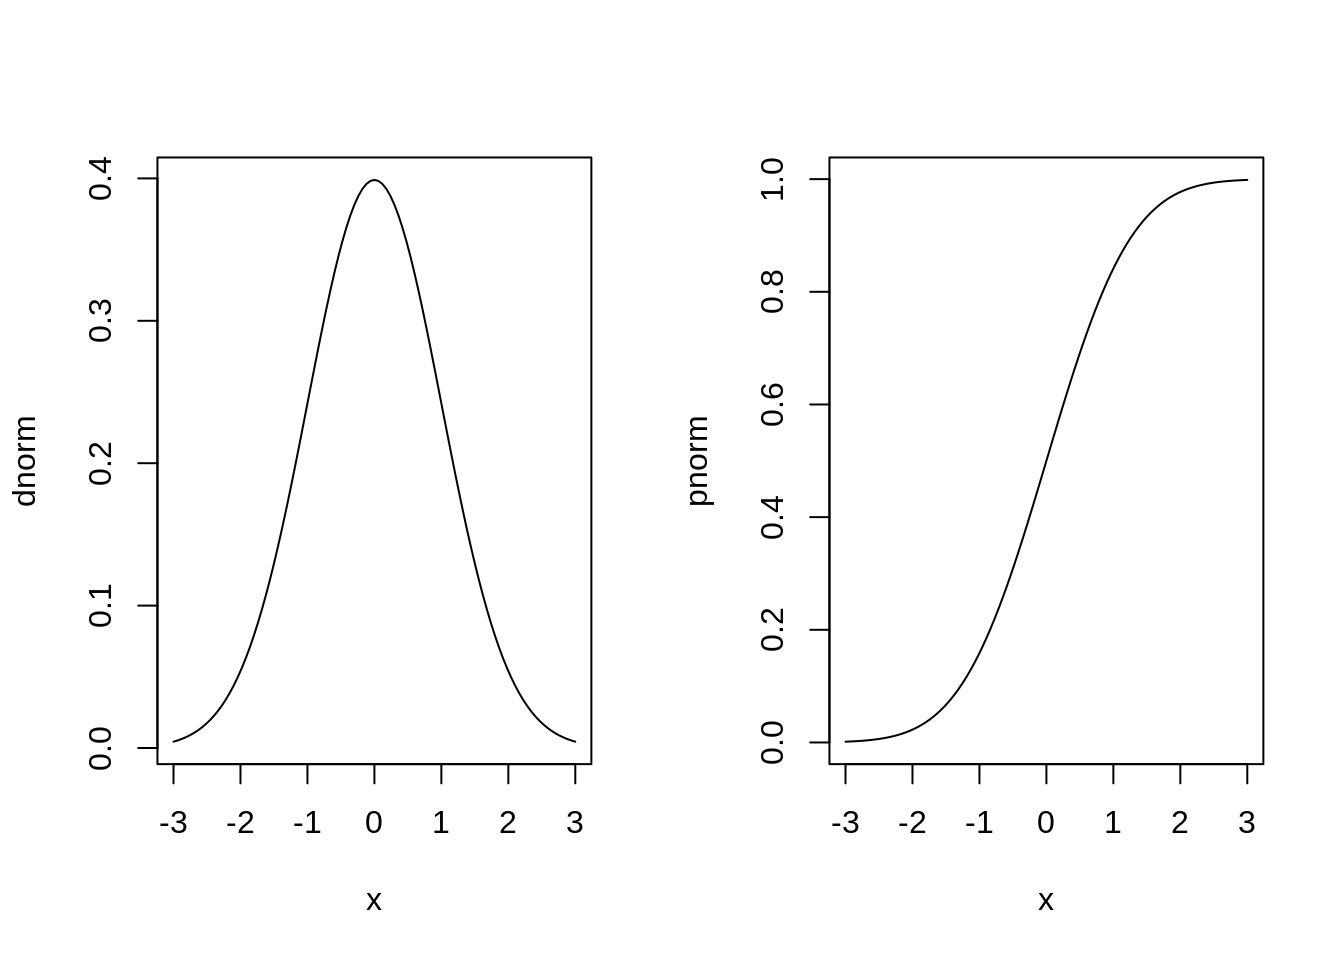
\includegraphics{figures/unnamed-chunk-342-1} \end{center}

\begin{quote}
VEJA a página de ajuda da função \texttt{plot.function()} para entender os
argumentos e demais funcionalidades desta função gráfica para plotar
gráficos de funções
\end{quote}

A seguinte figura mostra gráficos da densidade (esquerda) e
probabilidade acumulada (direita) da \(N(100, 64)\). Para fazer estes
gráficos tomamos uma sequência de valores de \(X\) entre 70 e 130 e para
cada um deles calculamos o valor das funções \(f(x)\) e \(F(x)\). Depois
unimos os pontos \((x,f(x))\) em um gráfico e \((x,F(x))\) no outro.

\begin{Shaded}
\begin{Highlighting}[]
\FunctionTok{par}\NormalTok{(}\AttributeTok{mfrow =} \FunctionTok{c}\NormalTok{(}\DecValTok{1}\NormalTok{, }\DecValTok{2}\NormalTok{))}
\NormalTok{x }\OtherTok{\textless{}{-}} \FunctionTok{seq}\NormalTok{(}\DecValTok{70}\NormalTok{, }\DecValTok{130}\NormalTok{, }\AttributeTok{length.out =} \DecValTok{100}\NormalTok{)}
\NormalTok{fx }\OtherTok{\textless{}{-}} \FunctionTok{dnorm}\NormalTok{(x, }\DecValTok{100}\NormalTok{, }\DecValTok{8}\NormalTok{)}
\FunctionTok{plot}\NormalTok{(x, fx, }\AttributeTok{type =} \StringTok{"l"}\NormalTok{)}
\NormalTok{Fx }\OtherTok{\textless{}{-}} \FunctionTok{pnorm}\NormalTok{(x, }\DecValTok{100}\NormalTok{, }\DecValTok{8}\NormalTok{)}
\FunctionTok{plot}\NormalTok{(x, Fx, }\AttributeTok{type =} \StringTok{"l"}\NormalTok{)}
\FunctionTok{par}\NormalTok{(}\AttributeTok{mfrow =} \FunctionTok{c}\NormalTok{(}\DecValTok{1}\NormalTok{, }\DecValTok{1}\NormalTok{))}
\end{Highlighting}
\end{Shaded}

\begin{center}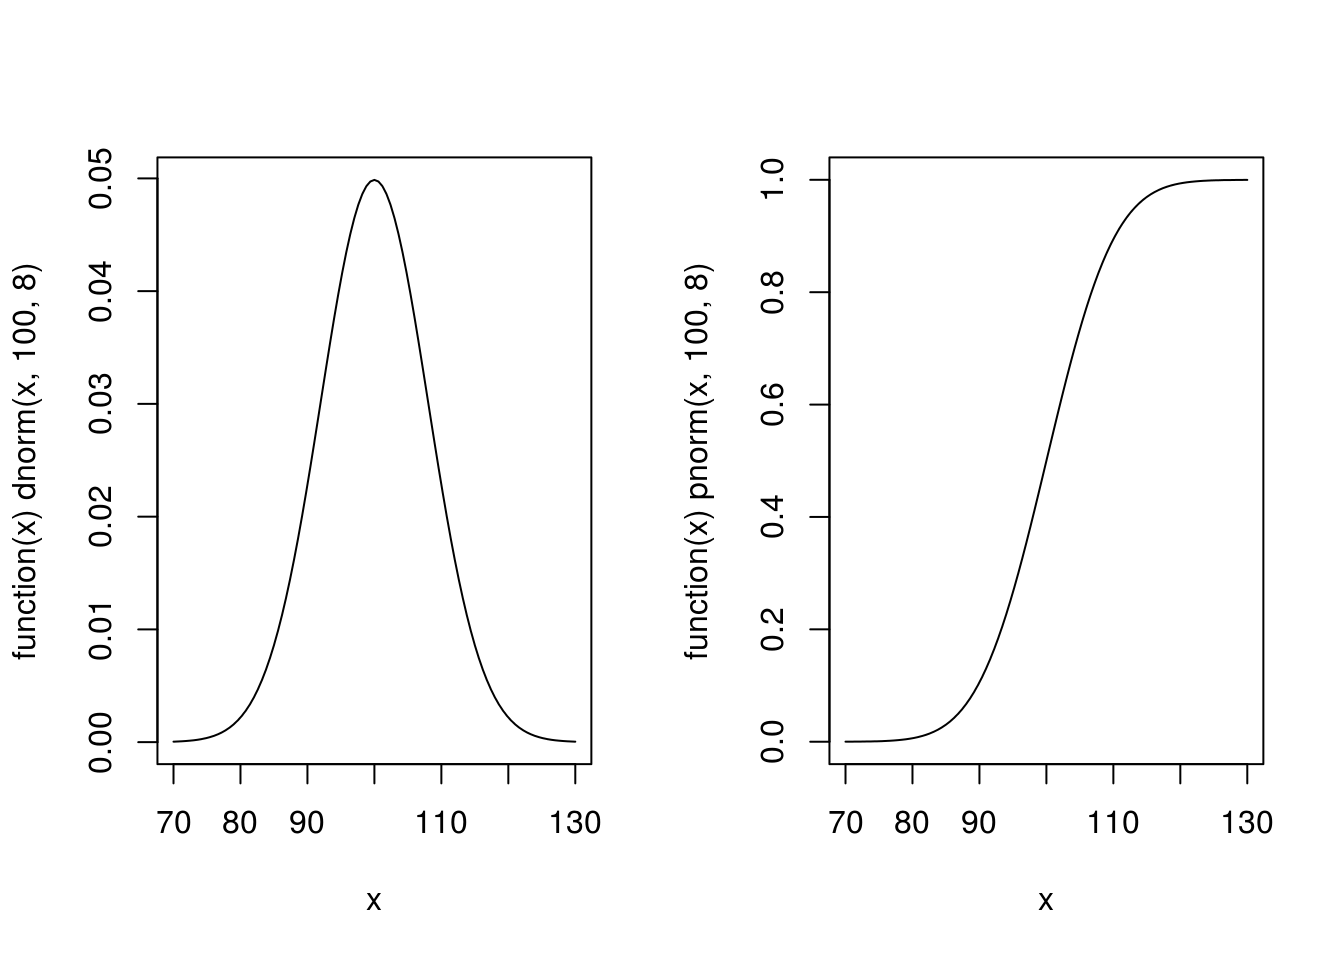
\includegraphics{figures/unnamed-chunk-343-1} \end{center}

Note que, alternativamente, os mesmos gráficos poderiam ser produzidos
com os comandos a seguir, onde fazemos usa da função \texttt{plot.function()}.

\begin{Shaded}
\begin{Highlighting}[]
\FunctionTok{par}\NormalTok{(}\AttributeTok{mfrow =} \FunctionTok{c}\NormalTok{(}\DecValTok{1}\NormalTok{, }\DecValTok{2}\NormalTok{))}
\FunctionTok{plot}\NormalTok{(}\ControlFlowTok{function}\NormalTok{(x) }\FunctionTok{dnorm}\NormalTok{(x, }\DecValTok{100}\NormalTok{, }\DecValTok{8}\NormalTok{), }\AttributeTok{from =} \DecValTok{70}\NormalTok{, }\AttributeTok{to =} \DecValTok{130}\NormalTok{)}
\FunctionTok{plot}\NormalTok{(}\ControlFlowTok{function}\NormalTok{(x) }\FunctionTok{pnorm}\NormalTok{(x, }\DecValTok{100}\NormalTok{, }\DecValTok{8}\NormalTok{), }\AttributeTok{from =} \DecValTok{70}\NormalTok{, }\AttributeTok{to =} \DecValTok{130}\NormalTok{)}
\FunctionTok{par}\NormalTok{(}\AttributeTok{mfrow =} \FunctionTok{c}\NormalTok{(}\DecValTok{1}\NormalTok{, }\DecValTok{1}\NormalTok{))}
\end{Highlighting}
\end{Shaded}

\begin{center}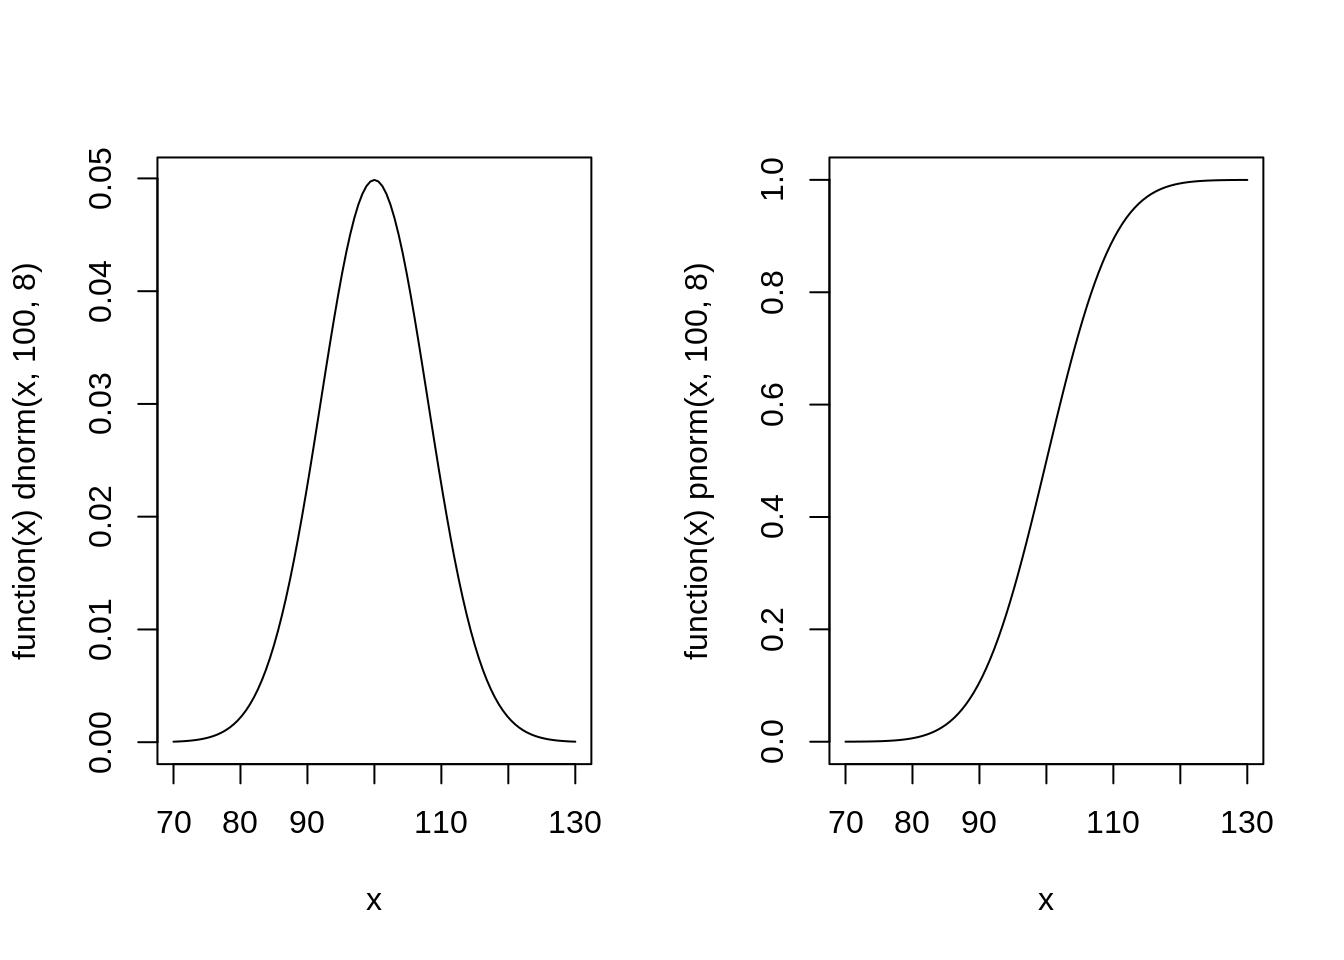
\includegraphics{figures/unnamed-chunk-344-1} \end{center}

Comandos usuais do R podem ser usados para modificar a aparência dos
gráficos. Por exemplo, podemos incluir títulos e mudar texto dos eixos
conforme mostrado abaixo.

\begin{Shaded}
\begin{Highlighting}[]
\FunctionTok{plot}\NormalTok{(dnorm, }\AttributeTok{from =} \SpecialCharTok{{-}}\DecValTok{3}\NormalTok{, }\AttributeTok{to =} \DecValTok{3}\NormalTok{,}
     \AttributeTok{xlab =} \StringTok{"Valores de X"}\NormalTok{,}
     \AttributeTok{ylab =} \StringTok{"Densidade de probabilidade"}\NormalTok{)}
\FunctionTok{title}\NormalTok{(}\StringTok{"Distribuicão Normal}\SpecialCharTok{\textbackslash{}n}\StringTok{X \textasciitilde{} N(0, 1)"}\NormalTok{)}
\end{Highlighting}
\end{Shaded}

\begin{center}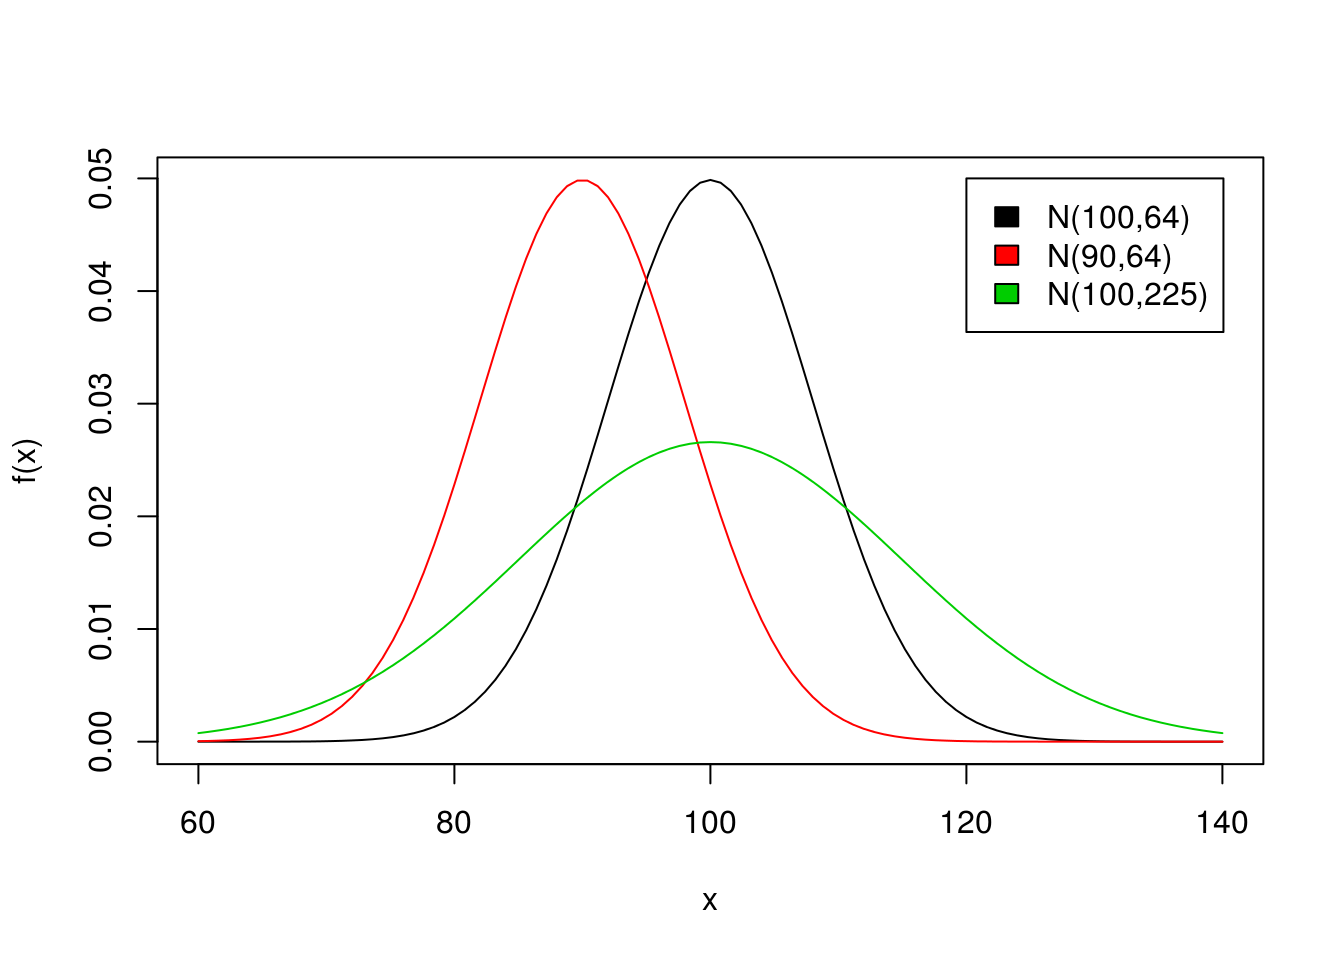
\includegraphics{figures/unnamed-chunk-345-1} \end{center}

Os demais comandos abaixo mostram como colocar diferentes densidades em um
mesmo gráfico, usando o argumento \texttt{add\ =\ TRUE}.

\begin{Shaded}
\begin{Highlighting}[]
\FunctionTok{plot}\NormalTok{(}\ControlFlowTok{function}\NormalTok{(x) }\FunctionTok{dnorm}\NormalTok{(x, }\DecValTok{100}\NormalTok{, }\DecValTok{8}\NormalTok{), }\DecValTok{60}\NormalTok{, }\DecValTok{140}\NormalTok{, }\AttributeTok{ylab =} \StringTok{\textquotesingle{}f(x)\textquotesingle{}}\NormalTok{)}
\FunctionTok{plot}\NormalTok{(}\ControlFlowTok{function}\NormalTok{(x) }\FunctionTok{dnorm}\NormalTok{(x, }\DecValTok{90}\NormalTok{, }\DecValTok{8}\NormalTok{), }\DecValTok{60}\NormalTok{, }\DecValTok{140}\NormalTok{, }\AttributeTok{add =} \ConstantTok{TRUE}\NormalTok{, }\AttributeTok{col =} \DecValTok{2}\NormalTok{)}
\FunctionTok{plot}\NormalTok{(}\ControlFlowTok{function}\NormalTok{(x) }\FunctionTok{dnorm}\NormalTok{(x, }\DecValTok{100}\NormalTok{, }\DecValTok{15}\NormalTok{), }\DecValTok{60}\NormalTok{, }\DecValTok{140}\NormalTok{, }\AttributeTok{add =} \ConstantTok{TRUE}\NormalTok{, }\AttributeTok{col =} \DecValTok{3}\NormalTok{)}
\FunctionTok{legend}\NormalTok{(}\DecValTok{120}\NormalTok{, }\FloatTok{0.05}\NormalTok{, }\AttributeTok{fill =} \DecValTok{1}\SpecialCharTok{:}\DecValTok{3}\NormalTok{,}
       \AttributeTok{legend =} \FunctionTok{c}\NormalTok{(}\StringTok{"N(100,64)"}\NormalTok{, }\StringTok{"N(90,64)"}\NormalTok{, }\StringTok{"N(100,225)"}\NormalTok{))}
\end{Highlighting}
\end{Shaded}

\begin{center}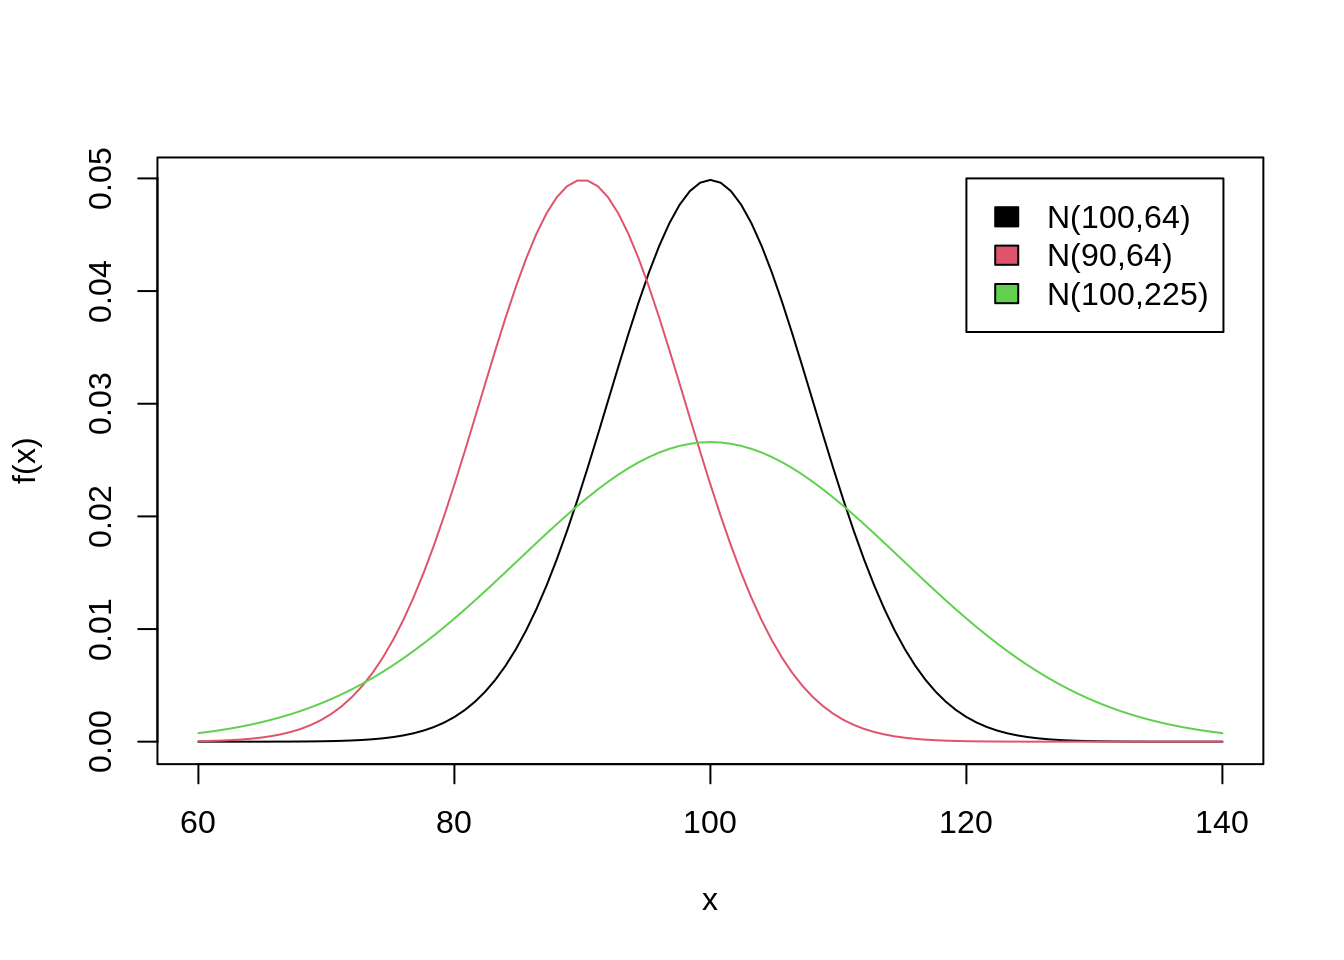
\includegraphics{figures/unnamed-chunk-346-1} \end{center}

\hypertarget{distribuiuxe7uxe3o-binomial}{%
\subsection{Distribuição Binomial}\label{distribuiuxe7uxe3o-binomial}}

Cálculos para a distribuição binomial são implementados combinando as
letras básicas vistas acima com o termo \texttt{binom}. Vamos primeiro
investigar os argumentos e a documentação com \texttt{args()} e \texttt{help()}.

\begin{Shaded}
\begin{Highlighting}[]
\FunctionTok{args}\NormalTok{(dbinom)}
\ControlFlowTok{function}\NormalTok{ (x, size, prob, }\AttributeTok{log =} \ConstantTok{FALSE}\NormalTok{) }
\ConstantTok{NULL}
\end{Highlighting}
\end{Shaded}

\begin{Shaded}
\begin{Highlighting}[]
\FunctionTok{help}\NormalTok{(dbinom)}
\end{Highlighting}
\end{Shaded}

Seja \(X\) uma v.a com distribuição binomial, com \(n=10\) e \(p=0.35\). Vamos
ver os comandos do R para:

\begin{itemize}
\tightlist
\item
  Fazer o gráfico da função de probabilidade.
\item
  Idem para a função de distribuição acumulada.
\item
  Calcular \(P(X = 7)\).
\item
  Calcular \(P(X \leq 7)\).
\item
  Calcular \(P(X > 7)\).
\item
  Calcular \(P(3 < X \leq 6)\).
\end{itemize}

Note que sendo uma distribuição discreta de probabilidades os gráficos
são diferentes dos obtidos para a distribuição normal e os cálculos de
probabilidades devem considerar as probabilidades nos pontos específicos.
Os gráficos das funções de probabilidade e distribuição são mostrados abaixo.

\begin{Shaded}
\begin{Highlighting}[]
\FunctionTok{par}\NormalTok{(}\AttributeTok{mfrow =} \FunctionTok{c}\NormalTok{(}\DecValTok{1}\NormalTok{, }\DecValTok{2}\NormalTok{))}
\NormalTok{x }\OtherTok{\textless{}{-}} \DecValTok{0}\SpecialCharTok{:}\DecValTok{10}
\NormalTok{fx }\OtherTok{\textless{}{-}} \FunctionTok{dbinom}\NormalTok{(x, }\AttributeTok{size =} \DecValTok{10}\NormalTok{, }\AttributeTok{prob =} \FloatTok{0.35}\NormalTok{)}
\FunctionTok{plot}\NormalTok{(x, fx, }\AttributeTok{type =} \StringTok{"h"}\NormalTok{)}
\NormalTok{Fx }\OtherTok{\textless{}{-}} \FunctionTok{pbinom}\NormalTok{(x, }\AttributeTok{size =} \DecValTok{10}\NormalTok{, }\AttributeTok{prob =} \FloatTok{0.35}\NormalTok{)}
\FunctionTok{plot}\NormalTok{(x, Fx, }\AttributeTok{type =} \StringTok{"s"}\NormalTok{)}
\FunctionTok{par}\NormalTok{(}\AttributeTok{mfrow =} \FunctionTok{c}\NormalTok{(}\DecValTok{1}\NormalTok{, }\DecValTok{1}\NormalTok{))}
\end{Highlighting}
\end{Shaded}

\begin{center}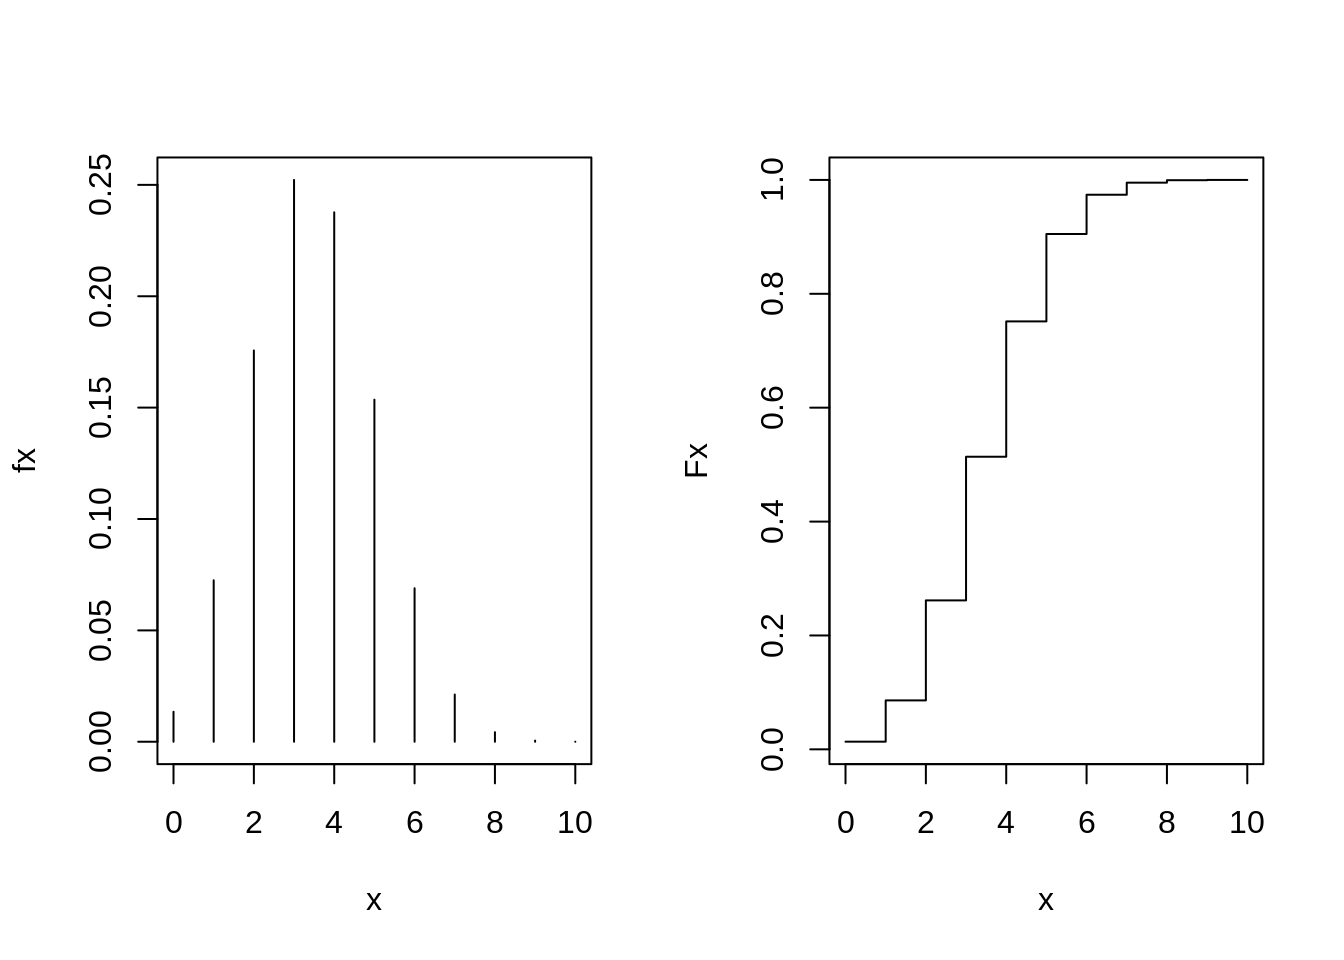
\includegraphics{figures/unnamed-chunk-349-1} \end{center}

As probabilidades pedidas são obtidas com os comandos a seguir.

\begin{Shaded}
\begin{Highlighting}[]
\DocumentationTok{\#\# P[X = 7]}
\FunctionTok{dbinom}\NormalTok{(}\DecValTok{7}\NormalTok{, }\AttributeTok{size =} \DecValTok{10}\NormalTok{, }\AttributeTok{prob =} \FloatTok{0.35}\NormalTok{)}
\NormalTok{[}\DecValTok{1}\NormalTok{] }\FloatTok{0.02120302}
\DocumentationTok{\#\# P[X \textless{}= 7]}
\FunctionTok{pbinom}\NormalTok{(}\DecValTok{7}\NormalTok{, }\AttributeTok{size =} \DecValTok{10}\NormalTok{, }\AttributeTok{prob =} \FloatTok{0.35}\NormalTok{)}
\NormalTok{[}\DecValTok{1}\NormalTok{] }\FloatTok{0.9951787}
\CommentTok{\# OU}
\FunctionTok{sum}\NormalTok{(}\FunctionTok{dbinom}\NormalTok{(}\DecValTok{0}\SpecialCharTok{:}\DecValTok{7}\NormalTok{, }\AttributeTok{size =} \DecValTok{10}\NormalTok{, }\AttributeTok{prob =} \FloatTok{0.35}\NormalTok{))}
\NormalTok{[}\DecValTok{1}\NormalTok{] }\FloatTok{0.9951787}
\DocumentationTok{\#\# P[X \textgreater{} 7]}
\DecValTok{1} \SpecialCharTok{{-}} \FunctionTok{pbinom}\NormalTok{(}\DecValTok{7}\NormalTok{, }\AttributeTok{size =} \DecValTok{10}\NormalTok{, }\AttributeTok{prob =} \FloatTok{0.35}\NormalTok{)}
\NormalTok{[}\DecValTok{1}\NormalTok{] }\FloatTok{0.004821265}
\FunctionTok{pbinom}\NormalTok{(}\DecValTok{7}\NormalTok{, }\AttributeTok{size =} \DecValTok{10}\NormalTok{, }\AttributeTok{prob =} \FloatTok{0.35}\NormalTok{, }\AttributeTok{lower.tail =} \ConstantTok{FALSE}\NormalTok{) }\CommentTok{\# melhor}
\NormalTok{[}\DecValTok{1}\NormalTok{] }\FloatTok{0.004821265}
\DocumentationTok{\#\# P[3 \textless{} X \textless{}= 6]}
\FunctionTok{pbinom}\NormalTok{(}\DecValTok{6}\NormalTok{, }\DecValTok{10}\NormalTok{, }\FloatTok{0.35}\NormalTok{) }\SpecialCharTok{{-}} \FunctionTok{pbinom}\NormalTok{(}\DecValTok{3}\NormalTok{, }\DecValTok{10}\NormalTok{, }\FloatTok{0.35}\NormalTok{)}
\NormalTok{[}\DecValTok{1}\NormalTok{] }\FloatTok{0.4601487}
\CommentTok{\# OU}
\FunctionTok{sum}\NormalTok{(}\FunctionTok{dbinom}\NormalTok{(}\DecValTok{4}\SpecialCharTok{:}\DecValTok{6}\NormalTok{, }\DecValTok{10}\NormalTok{, }\FloatTok{0.35}\NormalTok{))}
\NormalTok{[}\DecValTok{1}\NormalTok{] }\FloatTok{0.4601487}
\end{Highlighting}
\end{Shaded}

\hypertarget{distribuiuxe7uxe3o-de-poisson}{%
\subsection{Distribuição de Poisson}\label{distribuiuxe7uxe3o-de-poisson}}

\textbf{Definição:} Seja um experimento realizado nas seguintes
condições:
i. As ocorrências são independentes;
ii. As ocorrências são aleatórias;
iii. A variável aleatória \(X\) é o número de ocorrências de um
evento \textbf{ao longo de algum intervalo} (de tempo ou espaço);

Denominamos esse experimento de \textbf{processo de Poisson}. Vamos associar
a v.a \(X\) como sendo o número de ocorrências em um intervalo.
Portanto \(X\) poderá assumir os valores \(0, 1, \ldots,\) (sem limite superior).

A distribuição de Poisson é utilizada para descrever a probabilidade do \textbf{número de ocorrências} em um \textbf{intervalo contínuo} (de tempo ou espaço). No caso da distribuição binomial, a variável de interesse era o número de sucessos em um \textbf{intervalo discreto} (\(n\) ensaios de Bernoulli). A unidade de medida (tempo ou espaço) é uma variável contínua, mas a \emph{variável aleatória}, \textbf{número de ocorrências}, é discreta.

Uma v.a \(X\) segue o modelo de Poisson se surge a partir de um
processo de Poisson, e sua \textbf{função de probabilidade} for dada por

\[
P(X = x) = \frac{e^{-\mu} \mu^x}{x!}, \quad \quad x = 0, 1, \ldots
\]

onde

\[
\mu = \lambda \cdot t
\]

O parâmetro \(\mu\) indica a taxa de ocorrência (\(\lambda\)) por unidade
de medida (\(t\)), ou seja,

\[
    \lambda = \text{taxa de ocorrência} \quad \text{e} \quad t =
    \text{intervalo de tempo ou espaço}
\]

\begin{itemize}
\tightlist
\item
  Notação: \(X \sim \text{Pois}(\mu)\)
\item
  Esperança e variância: \(\text{E}(X) = \mu = \text{Var}(X)\)
\end{itemize}

Alguns exemplos de gráficos da distribuição de Poisson com diferentes
valores do parâmetro \(\mu\).

\begin{Shaded}
\begin{Highlighting}[]
\FunctionTok{par}\NormalTok{(}\AttributeTok{mfrow=}\FunctionTok{c}\NormalTok{(}\DecValTok{2}\NormalTok{,}\DecValTok{2}\NormalTok{))}
\FunctionTok{plot}\NormalTok{(}\DecValTok{0}\SpecialCharTok{:}\DecValTok{30}\NormalTok{, }\FunctionTok{dpois}\NormalTok{(}\AttributeTok{x =} \DecValTok{0}\SpecialCharTok{:}\DecValTok{30}\NormalTok{, }\AttributeTok{lambda =} \DecValTok{1}\NormalTok{), }\AttributeTok{type =} \StringTok{"h"}\NormalTok{,}
     \AttributeTok{xlab =} \StringTok{"X"}\NormalTok{, }\AttributeTok{ylab =} \StringTok{"P[X = x]"}\NormalTok{, }\AttributeTok{main =} \FunctionTok{expression}\NormalTok{(mu }\SpecialCharTok{==} \DecValTok{1}\NormalTok{),}
     \AttributeTok{ylim =} \FunctionTok{c}\NormalTok{(}\DecValTok{0}\NormalTok{,.}\DecValTok{4}\NormalTok{))}
\FunctionTok{plot}\NormalTok{(}\DecValTok{0}\SpecialCharTok{:}\DecValTok{30}\NormalTok{, }\FunctionTok{dpois}\NormalTok{(}\AttributeTok{x =} \DecValTok{0}\SpecialCharTok{:}\DecValTok{30}\NormalTok{, }\AttributeTok{lambda =} \DecValTok{5}\NormalTok{), }\AttributeTok{type =} \StringTok{"h"}\NormalTok{,}
     \AttributeTok{xlab =} \StringTok{"X"}\NormalTok{, }\AttributeTok{ylab =} \StringTok{"P[X = x]"}\NormalTok{, }\AttributeTok{main =} \FunctionTok{expression}\NormalTok{(mu }\SpecialCharTok{==} \DecValTok{5}\NormalTok{),}
     \AttributeTok{ylim =} \FunctionTok{c}\NormalTok{(}\DecValTok{0}\NormalTok{,.}\DecValTok{4}\NormalTok{))}
\FunctionTok{plot}\NormalTok{(}\DecValTok{0}\SpecialCharTok{:}\DecValTok{30}\NormalTok{, }\FunctionTok{dpois}\NormalTok{(}\AttributeTok{x =} \DecValTok{0}\SpecialCharTok{:}\DecValTok{30}\NormalTok{, }\AttributeTok{lambda =} \DecValTok{10}\NormalTok{), }\AttributeTok{type =} \StringTok{"h"}\NormalTok{,}
     \AttributeTok{xlab =} \StringTok{"X"}\NormalTok{, }\AttributeTok{ylab =} \StringTok{"P[X = x]"}\NormalTok{, }\AttributeTok{main =} \FunctionTok{expression}\NormalTok{(mu }\SpecialCharTok{==} \DecValTok{10}\NormalTok{),}
     \AttributeTok{ylim =} \FunctionTok{c}\NormalTok{(}\DecValTok{0}\NormalTok{,.}\DecValTok{4}\NormalTok{))}
\FunctionTok{plot}\NormalTok{(}\DecValTok{0}\SpecialCharTok{:}\DecValTok{30}\NormalTok{, }\FunctionTok{dpois}\NormalTok{(}\AttributeTok{x =} \DecValTok{0}\SpecialCharTok{:}\DecValTok{30}\NormalTok{, }\AttributeTok{lambda =} \DecValTok{15}\NormalTok{), }\AttributeTok{type =} \StringTok{"h"}\NormalTok{,}
     \AttributeTok{xlab =} \StringTok{"X"}\NormalTok{, }\AttributeTok{ylab =} \StringTok{"P[X = x]"}\NormalTok{, }\AttributeTok{main =} \FunctionTok{expression}\NormalTok{(mu }\SpecialCharTok{==} \DecValTok{15}\NormalTok{),}
     \AttributeTok{ylim =} \FunctionTok{c}\NormalTok{(}\DecValTok{0}\NormalTok{,.}\DecValTok{4}\NormalTok{))}
\end{Highlighting}
\end{Shaded}

\begin{center}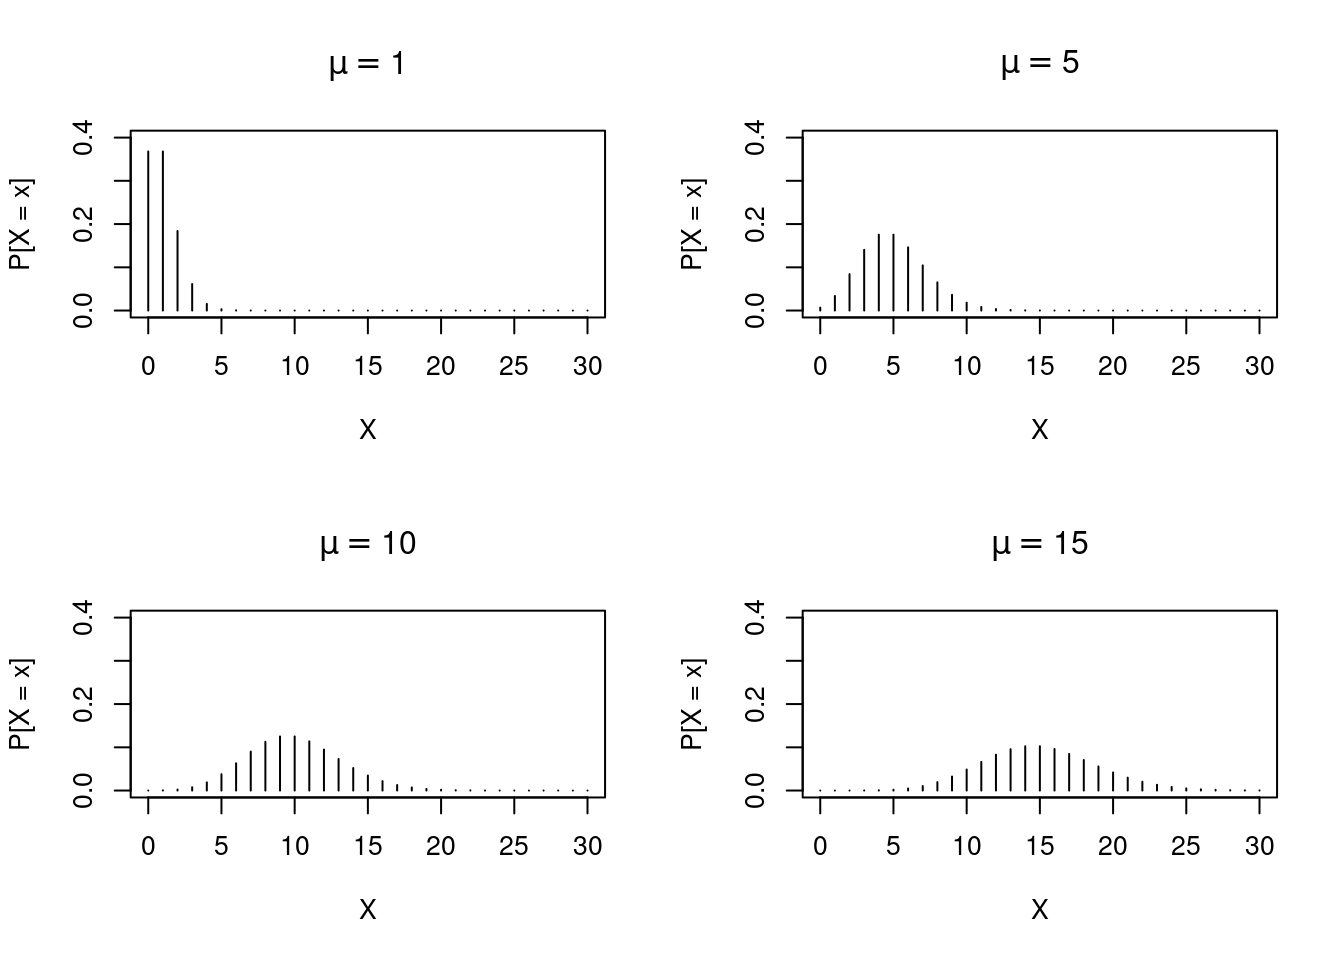
\includegraphics{figures/unnamed-chunk-351-1} \end{center}

\begin{itemize}
\tightlist
\item
  \textbf{Exemplo}: As chamadas telefônicas chegam a uma delegacia de
  polícia à uma taxa de 8 chamadas por hora, em dias úteis.

  \begin{enumerate}
  \def\labelenumi{\alph{enumi}.}
  \tightlist
  \item
    Quantas chamadas de emergência são esperadas em um período de 15 minutos?
  \item
    Qual a probabilidade de nenhuma chamada em um período de 15 minutos?
    c.~Qual a probabilidade de ocorrer pelo menos duas chamadas no período de 15 minutos?
    d.~Qual a probabilidade de ocorrer exatamente duas chamadas em 20 minutos?
  \end{enumerate}
\end{itemize}

\begin{Shaded}
\begin{Highlighting}[]
\DocumentationTok{\#\# a) E(X) = mu = lambda . t}
\NormalTok{lambda }\OtherTok{\textless{}{-}} \DecValTok{8}\SpecialCharTok{/}\DecValTok{60} \CommentTok{\# 8 chamadas/60 minutos}
\NormalTok{t }\OtherTok{\textless{}{-}} \DecValTok{15} \CommentTok{\# 15 minutos}
\NormalTok{(mu }\OtherTok{\textless{}{-}}\NormalTok{ lambda }\SpecialCharTok{*}\NormalTok{ t)}
\NormalTok{[}\DecValTok{1}\NormalTok{] }\DecValTok{2}
\DocumentationTok{\#\# b) P[x = 0]}
\FunctionTok{ppois}\NormalTok{(}\DecValTok{0}\NormalTok{, mu)}
\NormalTok{[}\DecValTok{1}\NormalTok{] }\FloatTok{0.1353353}
\FunctionTok{dpois}\NormalTok{(}\DecValTok{0}\NormalTok{, mu)}
\NormalTok{[}\DecValTok{1}\NormalTok{] }\FloatTok{0.1353353}
\DocumentationTok{\#\# c) P[X \textgreater{}= 2] = 1 {-} P[X \textless{} 2]}
\DecValTok{1} \SpecialCharTok{{-}} \FunctionTok{ppois}\NormalTok{(}\DecValTok{1}\NormalTok{, mu)}
\NormalTok{[}\DecValTok{1}\NormalTok{] }\FloatTok{0.5939942}
\FunctionTok{ppois}\NormalTok{(}\DecValTok{1}\NormalTok{, mu, }\AttributeTok{lower.tail =} \ConstantTok{FALSE}\NormalTok{)}
\NormalTok{[}\DecValTok{1}\NormalTok{] }\FloatTok{0.5939942}
\DocumentationTok{\#\# d) P[X = 2]}
\NormalTok{t }\OtherTok{\textless{}{-}} \DecValTok{20}
\NormalTok{(mu }\OtherTok{\textless{}{-}}\NormalTok{ lambda }\SpecialCharTok{*}\NormalTok{ t)}
\NormalTok{[}\DecValTok{1}\NormalTok{] }\FloatTok{2.666667}
\FunctionTok{dpois}\NormalTok{(}\DecValTok{2}\NormalTok{, mu)}
\NormalTok{[}\DecValTok{1}\NormalTok{] }\FloatTok{0.2470523}
\end{Highlighting}
\end{Shaded}

\begin{itemize}
\tightlist
\item
  \textbf{Exemplo:} Suponha que 150 erros de impressão são distribuídos aleatoriamente em um livro de 200 páginas. Encontre a probabilidade de que em 2 páginas contenham:

  \begin{enumerate}
  \def\labelenumi{\alph{enumi}.}
  \tightlist
  \item
    nenhum erro de impressão
  \item
    três erros de impressão
    c.~um ou mais erros de impressão
  \end{enumerate}
\end{itemize}

\begin{Shaded}
\begin{Highlighting}[]
\DocumentationTok{\#\# lambda = taxa de ocorrência por página}
\NormalTok{lambda }\OtherTok{\textless{}{-}} \DecValTok{150}\SpecialCharTok{/}\DecValTok{200}
\DocumentationTok{\#\# intervalo de interesse}
\NormalTok{t }\OtherTok{\textless{}{-}} \DecValTok{2}
\DocumentationTok{\#\# Parâmetro mu = lambda . t}
\NormalTok{(mu }\OtherTok{\textless{}{-}}\NormalTok{ lambda }\SpecialCharTok{*}\NormalTok{ t)}
\NormalTok{[}\DecValTok{1}\NormalTok{] }\FloatTok{1.5}
\DocumentationTok{\#\# a) P[X = 0]}
\FunctionTok{dpois}\NormalTok{(}\DecValTok{0}\NormalTok{, mu)}
\NormalTok{[}\DecValTok{1}\NormalTok{] }\FloatTok{0.2231302}
\DocumentationTok{\#\# b) P[X = 3]}
\FunctionTok{dpois}\NormalTok{(}\DecValTok{3}\NormalTok{, mu)}
\NormalTok{[}\DecValTok{1}\NormalTok{] }\FloatTok{0.1255107}
\DocumentationTok{\#\# c) P[X \textgreater{}= 1] = 1 {-} P[X \textless{} 1]}
\DecValTok{1} \SpecialCharTok{{-}} \FunctionTok{ppois}\NormalTok{(}\DecValTok{0}\NormalTok{, mu)}
\NormalTok{[}\DecValTok{1}\NormalTok{] }\FloatTok{0.7768698}
\FunctionTok{ppois}\NormalTok{(}\DecValTok{0}\NormalTok{, mu, }\AttributeTok{lower.tail =} \ConstantTok{FALSE}\NormalTok{)}
\NormalTok{[}\DecValTok{1}\NormalTok{] }\FloatTok{0.7768698}
\end{Highlighting}
\end{Shaded}

\hypertarget{distribuiuxe7uxe3o-uniforme}{%
\subsection{Distribuição Uniforme}\label{distribuiuxe7uxe3o-uniforme}}

\hypertarget{uniforme-contuxednua}{%
\subsubsection{Uniforme Contínua}\label{uniforme-contuxednua}}

Para a distribuição uniforme \emph{contínua} usa-se as funções \texttt{*unif()} onde
\texttt{*} deve ser \(p\), \(q\), \(d\) ou \(r\) como mencionado anteriormente. Nos
comandos a seguir inspecionamos os argumentos, sorteamos 5 valores da
\(U(0,1)\) e calculamos a probabilidade acumulada até 0,75.

\begin{Shaded}
\begin{Highlighting}[]
\FunctionTok{args}\NormalTok{(runif)}
\ControlFlowTok{function}\NormalTok{ (n, }\AttributeTok{min =} \DecValTok{0}\NormalTok{, }\AttributeTok{max =} \DecValTok{1}\NormalTok{) }
\ConstantTok{NULL}
\FunctionTok{runif}\NormalTok{(}\DecValTok{5}\NormalTok{)}
\NormalTok{[}\DecValTok{1}\NormalTok{] }\FloatTok{0.5358112} \FloatTok{0.7108038} \FloatTok{0.5383487} \FloatTok{0.7489722} \FloatTok{0.4201015}
\FunctionTok{punif}\NormalTok{(}\FloatTok{0.75}\NormalTok{)}
\NormalTok{[}\DecValTok{1}\NormalTok{] }\FloatTok{0.75}
\end{Highlighting}
\end{Shaded}

Portanto, o \emph{default} é uma distribuição uniforme no intervalo \([0,1]\)
e os argumentos opcionais são \texttt{min} e \texttt{max}. Por exemplo, para simular 5
valores de \(X \sim U(5, 20)\) usamos:

\begin{Shaded}
\begin{Highlighting}[]
\FunctionTok{runif}\NormalTok{(}\DecValTok{5}\NormalTok{, }\AttributeTok{min =} \DecValTok{5}\NormalTok{, }\AttributeTok{max =} \DecValTok{20}\NormalTok{)}
\NormalTok{[}\DecValTok{1}\NormalTok{]  }\FloatTok{7.571303} \FloatTok{16.554524} \FloatTok{18.229304} \FloatTok{13.236451}  \FloatTok{9.165856}
\end{Highlighting}
\end{Shaded}

\hypertarget{uniforme-discreta}{%
\subsubsection{Uniforme Discreta}\label{uniforme-discreta}}

Não há entre as funções básicas do R uma função específica para a
distribuição uniforme discreta com opções de prefixos \(r,d,p\) e \(d\),
provavelmente devido a sua simplicidade, embora algumas outras funções
possam ser usadas. Por exemplo para sortear números pode-se usar
\texttt{sample()}, como no exemplo a seguir onde são sorteados 15 valores de
uma uniforme discreta com valores (inteiros) entre 1 e 10 (\(X \sim U_d(1,10)\)).

\begin{Shaded}
\begin{Highlighting}[]
\FunctionTok{sample}\NormalTok{(}\DecValTok{1}\SpecialCharTok{:}\DecValTok{10}\NormalTok{, }\AttributeTok{size =} \DecValTok{15}\NormalTok{, }\AttributeTok{replace =} \ConstantTok{TRUE}\NormalTok{)}
\NormalTok{ [}\DecValTok{1}\NormalTok{] }\DecValTok{2} \DecValTok{3} \DecValTok{4} \DecValTok{4} \DecValTok{4} \DecValTok{5} \DecValTok{7} \DecValTok{9} \DecValTok{4} \DecValTok{2} \DecValTok{6} \DecValTok{7} \DecValTok{1} \DecValTok{6} \DecValTok{9}
\end{Highlighting}
\end{Shaded}

\hypertarget{a-funuxe7uxe3o-sample}{%
\subsection{\texorpdfstring{A função \texttt{sample()}}{A função sample()}}\label{a-funuxe7uxe3o-sample}}

A função \texttt{sample()} \textbf{não} é restrita à distribuição uniforme discreta,
podendo ser usada para sorteios, com ou sem reposição (argumento
\texttt{replace}, que por padrão é \texttt{FALSE}, ou seja, sem reposição), com a
possibilidade de associar diferentes probabilidades a cada elemento
(argumento \texttt{prob}, que por padrão associa probabilidades iguais para
todos os elementos).

\begin{Shaded}
\begin{Highlighting}[]
\FunctionTok{args}\NormalTok{(sample)}
\ControlFlowTok{function}\NormalTok{ (x, size, }\AttributeTok{replace =} \ConstantTok{FALSE}\NormalTok{, }\AttributeTok{prob =} \ConstantTok{NULL}\NormalTok{) }
\ConstantTok{NULL}
\end{Highlighting}
\end{Shaded}

Vejamos alguns exemplos:

\begin{itemize}
\tightlist
\item
  Sorteio de 3 números entre inteiros de 0 a 20.
\end{itemize}

\begin{Shaded}
\begin{Highlighting}[]
\FunctionTok{sample}\NormalTok{(}\DecValTok{0}\SpecialCharTok{:}\DecValTok{20}\NormalTok{, }\AttributeTok{size =} \DecValTok{3}\NormalTok{)}
\NormalTok{[}\DecValTok{1}\NormalTok{]  }\DecValTok{8} \DecValTok{20} \DecValTok{10}
\end{Highlighting}
\end{Shaded}

\begin{itemize}
\tightlist
\item
  Sorteio de 5 números entre os elementos de um certo vetor \texttt{x}.
\end{itemize}

\begin{Shaded}
\begin{Highlighting}[]
\NormalTok{x }\OtherTok{\textless{}{-}} \FunctionTok{c}\NormalTok{(}\DecValTok{23}\NormalTok{, }\DecValTok{34}\NormalTok{, }\DecValTok{12}\NormalTok{, }\DecValTok{22}\NormalTok{, }\DecValTok{17}\NormalTok{, }\DecValTok{28}\NormalTok{, }\DecValTok{18}\NormalTok{, }\DecValTok{19}\NormalTok{, }\DecValTok{20}\NormalTok{, }\DecValTok{13}\NormalTok{, }\DecValTok{18}\NormalTok{)}
\FunctionTok{sample}\NormalTok{(x, }\AttributeTok{size =} \DecValTok{5}\NormalTok{)}
\NormalTok{[}\DecValTok{1}\NormalTok{] }\DecValTok{18} \DecValTok{23} \DecValTok{20} \DecValTok{28} \DecValTok{22}
\end{Highlighting}
\end{Shaded}

\begin{itemize}
\tightlist
\item
  Sorteio de 10 números entre os possíveis resultados do lançamento de
  um dado, com reposição.
\end{itemize}

\begin{Shaded}
\begin{Highlighting}[]
\FunctionTok{sample}\NormalTok{(}\DecValTok{1}\SpecialCharTok{:}\DecValTok{6}\NormalTok{, }\AttributeTok{size =} \DecValTok{10}\NormalTok{, }\AttributeTok{replace =} \ConstantTok{TRUE}\NormalTok{)}
\NormalTok{ [}\DecValTok{1}\NormalTok{] }\DecValTok{6} \DecValTok{3} \DecValTok{5} \DecValTok{6} \DecValTok{3} \DecValTok{6} \DecValTok{4} \DecValTok{3} \DecValTok{3} \DecValTok{3}
\end{Highlighting}
\end{Shaded}

\begin{itemize}
\tightlist
\item
  Idem ao anterior, porém agora com a probabilidade de cada face proporcional
  ao valor da face.
\end{itemize}

\begin{Shaded}
\begin{Highlighting}[]
\FunctionTok{sample}\NormalTok{(}\DecValTok{1}\SpecialCharTok{:}\DecValTok{6}\NormalTok{, }\AttributeTok{size =} \DecValTok{10}\NormalTok{, }\AttributeTok{replace =} \ConstantTok{TRUE}\NormalTok{,  }\AttributeTok{prob =} \DecValTok{1}\SpecialCharTok{:}\DecValTok{6}\NormalTok{)}
\NormalTok{ [}\DecValTok{1}\NormalTok{] }\DecValTok{6} \DecValTok{4} \DecValTok{3} \DecValTok{6} \DecValTok{5} \DecValTok{3} \DecValTok{2} \DecValTok{6} \DecValTok{5} \DecValTok{5}
\end{Highlighting}
\end{Shaded}

Este último exemplo ilustra ainda que os valores passados para o
argumento \texttt{prob} não precisam ser probabilidades, são apenas entendidos
como \textbf{pesos}. A própria função trata isto internamente fazendo a
ponderação adequada.

\hypertarget{complementos-sobre-distribuiuxe7uxf5es-de-probabilidade}{%
\section{Complementos sobre distribuições de probabilidade}\label{complementos-sobre-distribuiuxe7uxf5es-de-probabilidade}}

Agora que já nos familiarizamos com o uso das distribuições de
probabilidade vamos ver alguns detalhes adicionais sobre seu
funcionamento.

\hypertarget{probabilidades-e-integrais}{%
\subsection{Probabilidades e integrais}\label{probabilidades-e-integrais}}

A probabilidade de um evento em uma distribuição contínua é a área sob
a curva da distribuição. Vamos reforçar esta idéia revisitando um
exemplo visto na distribuição normal.

Seja \(X\) uma v.a com distribuição \(N(100, 100)\). Para calcular a
probabilidade \(P(X < 95)\) usamos o comando:

\begin{Shaded}
\begin{Highlighting}[]
\FunctionTok{pnorm}\NormalTok{(}\DecValTok{95}\NormalTok{, }\AttributeTok{mean =} \DecValTok{100}\NormalTok{, }\AttributeTok{sd =} \DecValTok{10}\NormalTok{)}
\NormalTok{[}\DecValTok{1}\NormalTok{] }\FloatTok{0.3085375}
\end{Highlighting}
\end{Shaded}

Vamos agora ``esquecer'' o comando \texttt{pnorm()} e ver uma outra forma de
resolver usando integração numérica. Lembrando que a normal tem a função
de densidade dada por

\[
f(x) = \frac{1}{\sigma\sqrt{2 \pi}}\exp \left[ -\frac{1}{2}
    \left( \frac{x - \mu}{\sigma} \right)^2 \right].
\]

Podemos então definir uma função no R para calcular qualquer densidade
em \(x\)

\begin{Shaded}
\begin{Highlighting}[]
\NormalTok{fn }\OtherTok{\textless{}{-}} \ControlFlowTok{function}\NormalTok{(x, mu, sigma)\{}
\NormalTok{    (}\DecValTok{1}\SpecialCharTok{/}\NormalTok{(sigma }\SpecialCharTok{*} \FunctionTok{sqrt}\NormalTok{(}\DecValTok{2}\SpecialCharTok{*}\NormalTok{pi))) }\SpecialCharTok{*} \FunctionTok{exp}\NormalTok{((}\SpecialCharTok{{-}}\DecValTok{1}\SpecialCharTok{/}\DecValTok{2}\NormalTok{) }\SpecialCharTok{*}\NormalTok{ ((x }\SpecialCharTok{{-}}\NormalTok{ mu)}\SpecialCharTok{/}\NormalTok{sigma)}\SpecialCharTok{\^{}}\DecValTok{2}\NormalTok{)}
\NormalTok{\}}
\end{Highlighting}
\end{Shaded}

Para obter o gráfico desta distribuição, usamos o fato que
a maior parte da massa da função está no intervalo entre a média +/- três
desvios padrões, portanto entre 70 e 130. Podemos então fazer como nos
comandos que se seguem. Para marcar no gráfico a área que corresponde a
probabilidade pedida criamos um polígono com coordenadas \texttt{ax} e \texttt{ay}
definindo o perímetro desta área.

\begin{Shaded}
\begin{Highlighting}[]
\NormalTok{x }\OtherTok{\textless{}{-}} \FunctionTok{seq}\NormalTok{(}\DecValTok{70}\NormalTok{, }\DecValTok{130}\NormalTok{, }\AttributeTok{length.out =} \DecValTok{200}\NormalTok{)}
\NormalTok{fx }\OtherTok{\textless{}{-}} \FunctionTok{fn}\NormalTok{(x, }\AttributeTok{mu =} \DecValTok{100}\NormalTok{, }\AttributeTok{sigma =} \DecValTok{10}\NormalTok{)}
\FunctionTok{plot}\NormalTok{(x, fx, }\AttributeTok{type =} \StringTok{"l"}\NormalTok{)}
\NormalTok{ax }\OtherTok{\textless{}{-}} \FunctionTok{c}\NormalTok{(}\DecValTok{70}\NormalTok{, }\DecValTok{70}\NormalTok{, x[x }\SpecialCharTok{\textless{}} \DecValTok{95}\NormalTok{], }\DecValTok{95}\NormalTok{, }\DecValTok{95}\NormalTok{)}
\NormalTok{ay }\OtherTok{\textless{}{-}} \FunctionTok{c}\NormalTok{(}\DecValTok{0}\NormalTok{, }\FunctionTok{fn}\NormalTok{(}\DecValTok{70}\NormalTok{, }\DecValTok{100}\NormalTok{, }\DecValTok{10}\NormalTok{), fx[x }\SpecialCharTok{\textless{}} \DecValTok{95}\NormalTok{], }\FunctionTok{fn}\NormalTok{(}\DecValTok{95}\NormalTok{, }\DecValTok{100}\NormalTok{, }\DecValTok{10}\NormalTok{),}\DecValTok{0}\NormalTok{)}
\FunctionTok{polygon}\NormalTok{(ax, ay, }\AttributeTok{density =} \DecValTok{10}\NormalTok{)}
\end{Highlighting}
\end{Shaded}

\begin{center}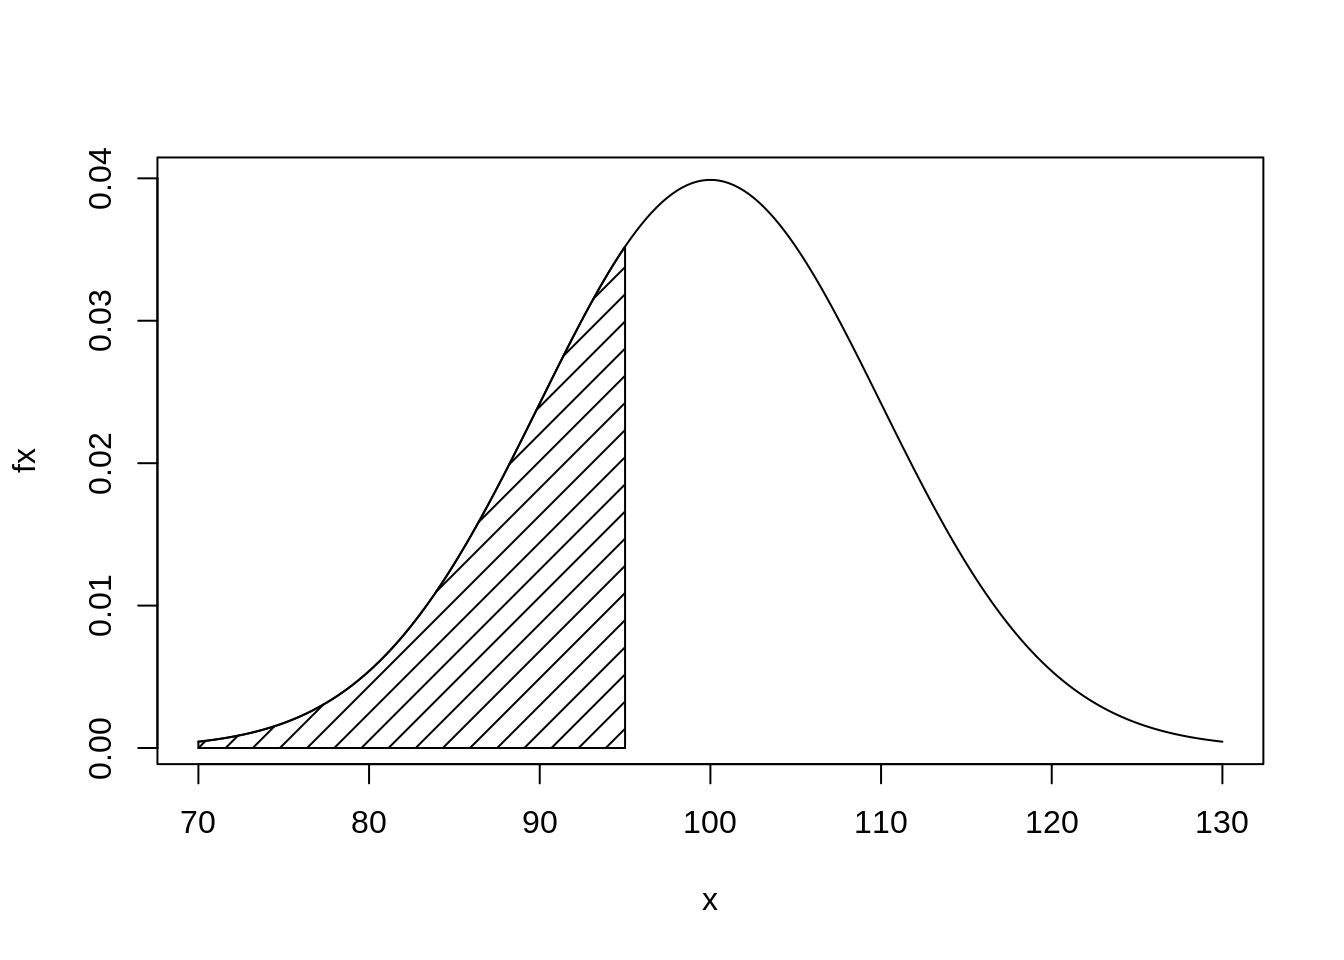
\includegraphics{figures/unnamed-chunk-364-1} \end{center}

Para calcular a área pedida sem usar a função \texttt{pnorm()} podemos usar a
função de integração numérica. Note que esta função, diferentemente da
\texttt{pnorm()} reporta ainda o erro de aproximação numérica.

\begin{Shaded}
\begin{Highlighting}[]
\FunctionTok{integrate}\NormalTok{(fn, }\AttributeTok{mu =} \DecValTok{100}\NormalTok{, }\AttributeTok{sigma =} \DecValTok{10}\NormalTok{, }\AttributeTok{lower =} \SpecialCharTok{{-}}\ConstantTok{Inf}\NormalTok{, }\AttributeTok{upper =} \DecValTok{95}\NormalTok{)}
\FloatTok{0.3085375}\NormalTok{ with absolute error }\SpecialCharTok{\textless{}} \FloatTok{2.1e{-}06}
\end{Highlighting}
\end{Shaded}

Portanto para os demais ítens do problema, \(P(90 < X < 110)\), e
\(P(X > 95)\) fazemos:

\begin{Shaded}
\begin{Highlighting}[]
\FunctionTok{integrate}\NormalTok{(fn, }\AttributeTok{mu =} \DecValTok{100}\NormalTok{, }\AttributeTok{sigma =} \DecValTok{10}\NormalTok{, }\AttributeTok{lower =} \DecValTok{90}\NormalTok{, }\AttributeTok{upper =} \DecValTok{110}\NormalTok{)}
\FloatTok{0.6826895}\NormalTok{ with absolute error }\SpecialCharTok{\textless{}} \FloatTok{7.6e{-}15}
\FunctionTok{integrate}\NormalTok{(fn, }\AttributeTok{mu =} \DecValTok{100}\NormalTok{, }\AttributeTok{sigma =} \DecValTok{10}\NormalTok{, }\AttributeTok{lower =} \DecValTok{95}\NormalTok{, }\AttributeTok{upper =} \SpecialCharTok{+}\ConstantTok{Inf}\NormalTok{)}
\FloatTok{0.6914625}\NormalTok{ with absolute error }\SpecialCharTok{\textless{}} \FloatTok{8.1e{-}05}
\end{Highlighting}
\end{Shaded}

e os resultados acima evidentemente coincidem com os obtidos
anterioriormente usando \texttt{pnorm()},

\begin{Shaded}
\begin{Highlighting}[]
\FunctionTok{pnorm}\NormalTok{(}\DecValTok{110}\NormalTok{, }\DecValTok{100}\NormalTok{, }\DecValTok{10}\NormalTok{) }\SpecialCharTok{{-}} \FunctionTok{pnorm}\NormalTok{(}\DecValTok{90}\NormalTok{, }\DecValTok{100}\NormalTok{, }\DecValTok{10}\NormalTok{)}
\NormalTok{[}\DecValTok{1}\NormalTok{] }\FloatTok{0.6826895}
\FunctionTok{pnorm}\NormalTok{(}\DecValTok{95}\NormalTok{, }\DecValTok{100}\NormalTok{, }\DecValTok{10}\NormalTok{, }\AttributeTok{lower.tail =} \ConstantTok{FALSE}\NormalTok{)}
\NormalTok{[}\DecValTok{1}\NormalTok{] }\FloatTok{0.6914625}
\end{Highlighting}
\end{Shaded}

Note ainda que na prática não precisamos definir e usar a função \texttt{fn()},
pois ela fornece o mesmo resultado que a função \texttt{dnorm()}.

\hypertarget{exercuxedcios-17}{%
\section*{Exercícios}\label{exercuxedcios-17}}


Nos exercícios abaixo iremos também usar o R como uma calculadora
estatística para resolver alguns exemplos/exercícios de probabilidade
tipicamente apresentados em um curso de estatística básica.

\begin{enumerate}
\def\labelenumi{\arabic{enumi}.}
\tightlist
\item
  Para \(X \sim N(90, 100)\), obtenha:

  \begin{enumerate}
  \def\labelenumii{\alph{enumii}.}
  \tightlist
  \item
    \(P(X \leq 115)\).
  \item
    \(P(X \geq 80)\).
  \item
    \(P(X \leq 75)\).
  \item
    \(P(85 \leq X \leq 110)\).
  \item
    \(P(|X - 90| \leq 10)\).
  \item
    O valor de \(a\) tal que \(P(90-a \leq X \leq 90+a) = 0.95\).
  \end{enumerate}
\item
  Sendo \(X\) uma variável seguindo o modelo
  Binomial com parâmetros \(n = 15\) e \(p = 0.4\), pergunta-se:

  \begin{enumerate}
  \def\labelenumii{\alph{enumii}.}
  \tightlist
  \item
    \(P(X \geq 14)\).
  \item
    \(P(8 < X \leq 10)\).
  \item
    \(P(X < 2 \; \mbox{ ou } \;\; X \geq 11)\).
  \item
    \(P(X \geq 11 \; \mbox{ ou } \;\; X > 13)\).
  \item
    \(P(X > 3 \; \mbox{ e } \;\; X < 6)\).
  \item
    \(P(X \leq 13 \; | \; X \geq 11)\).
  \end{enumerate}
\item
  Uma empresa informa que 30\% de suas contas a receber de outras empresas encontram-se vencidas. Se o contador da empresa seleciona aleatoriamente 5 contas, determine a probabilidade de:

  \begin{enumerate}
  \def\labelenumii{\alph{enumii}.}
  \tightlist
  \item
    Nenhuma conta estar vencida
  \item
    Exatamente duas contas estarem vencidas
  \item
    Três ou mais contas estarem vencidas
  \end{enumerate}
\item
  Uma empresa recebe 720 emails em um intervalo de 8 horas. Qual a probabilidade de que:

  \begin{enumerate}
  \def\labelenumii{\alph{enumii}.}
  \tightlist
  \item
    Em 6 minutos receba pelo menos 3 emails?
  \item
    Em 4 minutos não receba nenhum email?
  \end{enumerate}
\item
  O processo de empacotamento de uma fábrica de cereais foi ajustado de maneira que uma média de \(\mu = 13,0\) kg de cereal seja colocado em cada caixa. Sabe-se que existe uma pequena variabilidade no enchimento dos pacotes devido à fatores aleatórios, e que o desvio-padrão do peso de enchimento é de \(\sigma = 0,1\) kg. Assume-se que a distribuição dos pesos tem distribuição normal. Com isso, determine as probabilidades de que uma caixa escolhida ao acaso:

  \begin{enumerate}
  \def\labelenumii{\alph{enumii}.}
  \tightlist
  \item
    Pese entre 13,0 e 13,2 kg.
  \item
    Tenha um peso maior do que 13,25 kg.
  \item
    Pese entre 12,8 e 13,1 kg.
  \item
    Pese entre 13,1 e 13,2 kg.
  \end{enumerate}
\item
  Faça os seguintes gráficos:

  \begin{enumerate}
  \def\labelenumii{\alph{enumii}.}
  \tightlist
  \item
    da função de densidade de uma variável com distribuição de Poisson com parâmetro \(\lambda = 5\).
  \item
    da densidade de uma variável \(X \sim N(90, 100)\).
  \item
    sobreponha ao gráfico anterior a densidade de uma variável \(Y \sim N(90, 80)\) e outra \(Z \sim N(85, 100)\).
  \item
    densidades de distribuições \(\chi^2\) com 1, 2 e 5 graus de liberdade.
  \end{enumerate}
\end{enumerate}

\hypertarget{inferuxeancia-estatuxedstica}{%
\chapter{Inferência estatística}\label{inferuxeancia-estatuxedstica}}

\hypertarget{introduuxe7uxe3o-ao-pensamento-estatuxedstico}{%
\section{Introdução ao pensamento estatístico}\label{introduuxe7uxe3o-ao-pensamento-estatuxedstico}}

No contexto de análise e modelagem estatística o analista assume que todos os fenômenos aleatórios podem ser representados por distribuições de probabilidades, ou seja, um modelo estatístico. Tais distribuições são representações de como a variável aleatória deve se comportar na população. Em cursos de inferência estatística é usual a frase `'seja X uma variável aleatória de uma população normal com média \(\mu\) e variância \(\sigma^2\)''.
Essa frase exemplifica a forma como o estatístico supõe que um certo fenômeno aleatório se comporta na população.

Considere o caso de uma pesquisa eleitoral onde potenciais eleitores são entrevistados sobre a sua intenção em votar (SUCESSO) ou não votar (FRACASSO) em um determinado candidato X. Note que pela estrutura do fenômeno aleatório o modelo Bernoulli é um candidato natural para modelar o comportamento da variável aleatória `'intenção de voto''.
Suponha ainda que um conjunto de \(n\) eleitores vão ser entrevistados e que a probabilidade de sucesso, ou seja, votar no candidato X seja constante para todos os entrevistados e denotada por \(p.\) Nestas condições podemos estar interessados na variável aleatória Y que conta o número de sucessos (eleitores que vão votar em X) entre \(n\) eleitores. Sendo assim, a distribuição de probabilidade de \(Y\) é binomial com parâmetros \(n\) e \(p\) e sua função de probabilidade é dada por

\[
P(Y = y) = P(Y = y) = \binom{n}{y} p^y (1-p)^{n-y}.
\]
Note que esta distribuição é completamente governada pelos valores de seus parâmetros, ou seja, \(n\) e \(p\). Em geral \(n\) é fixado e conhecido, por outro lado \(p\) é desconhecido. Em termos práticos, o valor de \(p\) é o que estamos interessados, uma vez que ele representa a proporção populacional de eleitores do candidato \(X\).

Se fossemos capazes de entrevistar todos os elementos da população de interesse, poderíamos facilmente calcular a proporção de eleitores de \(X\) e plugar no modelo para calcular quaisquer tipos de probabilidades de interesse. No entanto na prática, muitas vezes entrevistar todos os elementos da população de interesse é impossível ou extremamente custoso. Nestas situações o problema que surge é como que baseado apenas em uma amostra da população de interesse podemos falar algo sobre toda a população. Este é o problema de uma das áreas da estatística chamada de inferência estatística.

O objetivo deste texto não é discutir inferência estatística em detalhes, mas apenas apresentar as principais ideias e ilustrar a sua implementação computacional utilizando o software R. Além disso, uma série de procedimentos pré-prontos estão disponíveis em R e devem ser apresentados de forma breve, uma vez que as ideias são similares apenas adaptadas à situações específicas.

O processo de inferência estatística começa com a especificação de uma distribuição de probabilidade para a variável aleatória de interesse. Neste caso, vamos definir a variável de interesse como sendo \(Y\) - votar no candidato X. Note que esta é uma v.a binária, ou seja, apresenta apenas os valores \(0\)-não vai votar no candidato X ou \(1\) vai votar no candidato X. Neste caso, podemos especificar que \(Y \sim B(p)\), ou seja, \(Y\) segue o modelo de Bernoulli com parâmetro \(p\). Importante lembrar que o espaço paramétrico de \(p\) neste caso é o intervalo unitário, ou seja, \(p \in (0,1)\).

Uma vez com o modelo especificado precisamos de informações sobre o parâmetro populacional de interesse, neste caso \(p\) que representa a proporção de eleitores do candidato X. Para obter informações sobre \(p\) vamos coletar uma amostra da população de interesse e medir a variável de interesse. Neste caso, isso significa simplesmente perguntar se o eleitor vai ou não votar no candidato X. Em R podemos facilmente simular esta situação prática usando a função \(rbinom()\), conforme ilustra o código abaixo

\begin{Shaded}
\begin{Highlighting}[]
\FunctionTok{set.seed}\NormalTok{(}\DecValTok{123}\NormalTok{)}
\NormalTok{y }\OtherTok{\textless{}{-}} \FunctionTok{rbinom}\NormalTok{(}\AttributeTok{n =} \DecValTok{10}\NormalTok{, }\AttributeTok{size =} \DecValTok{1}\NormalTok{, }\AttributeTok{prob =} \FloatTok{0.5}\NormalTok{)}
\NormalTok{y}
\NormalTok{ [}\DecValTok{1}\NormalTok{] }\DecValTok{0} \DecValTok{1} \DecValTok{0} \DecValTok{1} \DecValTok{1} \DecValTok{0} \DecValTok{1} \DecValTok{1} \DecValTok{1} \DecValTok{0}
\end{Highlighting}
\end{Shaded}

Note que para simular uma amostra nós precisamos especificar o tamanho da amostra, neste caso \(n=10\) o número de ensaios Bernoulli neste caso apenas \(1\) e a probabilidade de sucesso (proporção populacional). É claro que na prática a proporção populacional é desconhecida, mas neste caso fixamos um valor para simular observações e o objetivo é apenas baseado nas realizações da variável aleatória \textbf{descobrir} ou \textbf{inferir} qual é o verdadeiro valor de \(p\). De forma mais geral os objetivos da inferência estatística são:

\begin{itemize}
\tightlist
\item
  Estimar \(p\) baseado apenas na amostra (valor pontual)! Pense que deseja-se responder a pergunta: Quanto você acha que é a proporção de eleitores do candidato X na população?
\item
  Informar o quanto você acredita no valor estimado (intervalo de confiança).
\item
  Decidir sobre possíveis valores de p baseado apenas na amostra. Por exemplo, O candidato X vai ganhar (p \textgreater{} 0,50)?
\end{itemize}

Interessante notar que até este momento não fizemos nenhuma suposição em como as observações foram obtidas. No entanto, se supomos que as observações são independentes podemos facilmente obter a distribuição conjunta de todas as variáveis aleatórias envolvidas no modelo como o produto da distribuição de cada uma. Neste caso, todas as observações vêm de uma população Bernoulli com parâmetro \(p\). Assim, a distribuição conjunta é dada pelo seguinte produtório

\[
P(Y = y) = \prod_{i=1}^{n} p^{y_i} (1-p)^{1-y_i} = p^{\sum_{i=1}^n y_i} (1-p)^{n - \sum_{i=1}^n y_i}.
\]
Uma forma alternativa é escrever a distribuição do número de sucessos em \(n\) ensaios Bernoulli que é simplesmente uma distribuição binomial com parâmetros \(n\) e \(p\), ou seja,

\[
P(Y = y) = P(Y = y) = \binom{n}{y} p^y (1-p)^{n-y}.
\]
É importante enfatizar que após a amostra ser coletada o número \(y\) de sucesso é fixo. Para a nossa amostra, temos \(y = 6\). Lembre-se que o \(n\) foi fixado, assim para avaliar a equação acima em algum ponto, só precisamos fixar o valor de \(p\).

Agora vamos refletir sobre o que a equação acima está nos fornecendo. Suponha que em um primeiro momento você apenas precise decidir se \(p = 0.5\) ou \(p = 0.8\). Como poderíamos usar o nosso modelo para tomar esta decisão?

Note que podemos calcular qual é a probabilidade de obter \(6\) sucessos em \(n\) ensaios supondo que \(p = 0.5\) e também supondo que \(p = 0.8\). Vamos fazer estas contas

\[
P(Y = 6 | p = 0.5) = \binom{10}{6} 0.5^6 (1-0.5)^{10-6} = 0.205.
\]
\[
P(Y = 6 | p = 0.8) = \binom{10}{6} 0.8^6 (1-0.8)^{10-6} = 0.088.
\]
Em R temos,

\begin{Shaded}
\begin{Highlighting}[]
\FunctionTok{dbinom}\NormalTok{(}\DecValTok{6}\NormalTok{, }\AttributeTok{size =} \DecValTok{10}\NormalTok{, }\AttributeTok{prob =} \FloatTok{0.5}\NormalTok{)}
\NormalTok{[}\DecValTok{1}\NormalTok{] }\FloatTok{0.2050781}
\FunctionTok{dbinom}\NormalTok{(}\DecValTok{6}\NormalTok{, }\AttributeTok{size =} \DecValTok{10}\NormalTok{, }\AttributeTok{prob =} \FloatTok{0.8}\NormalTok{)}
\NormalTok{[}\DecValTok{1}\NormalTok{] }\FloatTok{0.08808038}
\end{Highlighting}
\end{Shaded}

Baseado apenas nestas probabilidades, é possível observar que a probabilidade de observarmos \(6\) sucessos em \(10\) ensaios é mais provável quando \(p = 0.5\) do que quando \(p = 0.8\). Neste caso podemos concluir que existe mais evidências em favor de \(p=0.5\) do que em favor de \(p = 0.8\). Veja que fizemos uma espécie de pensamento inverso, observamos \(6\) sucessos e agora estamos pensando, qual é o valor de \(p\) mais compatível com esse valor. Além disso, a função de probabilidade conjunta vista como uma função do parâmetro ao invés da variável aleatória nos fornece exatamente essa noção de compatibilidade, ou seja, qual é o valor de \(p\) mais compatível com as minhas observações.

Para enfatizar esta idéia vamos rescrever a função acima para enfatizar que a quantidade desconhecida agora é \(p\) e não mais \(y\).

\[
L(p|y) = \binom{n}{y} p^y (1-p)^{n-y}.
\]
A função acima é chamada de \textbf{verossimilhança} e é fundamental em todo o processo de inferência estatística. No caso de variáveis aleatórias discretas ela nos fornece a probabilidade de observar o que realmente foi observado dado um particular valor para o parâmetro de interesse. Particularizando para o nosso exemplo temos

\[
L(p|y) = \binom{10}{6} p^6 (1-p)^{10-6}.
\]
Como dito a função de verossimilhança nos fornece uma medida de compatibilidade de um particular valor de \(p\) com a amostra observada. Assim, é natural tomarmos como o nosso melhor `'chute'' o valor mais compatível com a amostra observada, ou seja, o ponto de máximo da função de verossimilhança. Vamos fazer um gráfico para ilustrar esta ideia.

\begin{Shaded}
\begin{Highlighting}[]
\NormalTok{L }\OtherTok{\textless{}{-}} \ControlFlowTok{function}\NormalTok{(p, n, y) \{}
\NormalTok{  out }\OtherTok{\textless{}{-}} \FunctionTok{dbinom}\NormalTok{(y, }\AttributeTok{size =}\NormalTok{ n, }\AttributeTok{prob =}\NormalTok{ p)}
  \FunctionTok{return}\NormalTok{(out)}
\NormalTok{\}}
\FunctionTok{curve}\NormalTok{(}\FunctionTok{L}\NormalTok{(x, }\AttributeTok{n =} \DecValTok{10}\NormalTok{, }\AttributeTok{y =} \DecValTok{6}\NormalTok{), }\DecValTok{0}\NormalTok{, }\DecValTok{1}\NormalTok{)}
\end{Highlighting}
\end{Shaded}

\begin{center}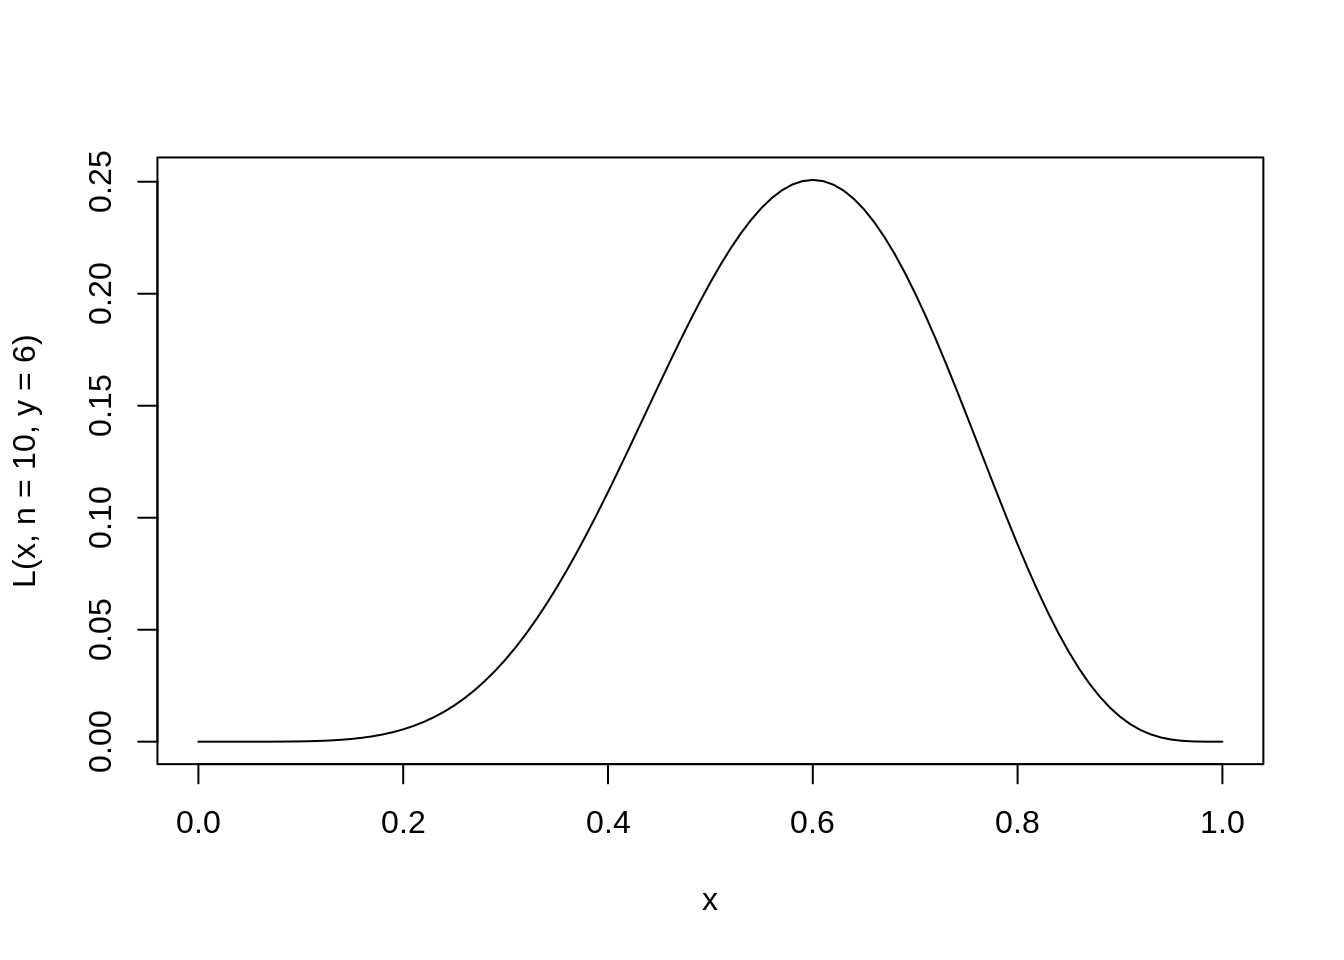
\includegraphics{figures/unnamed-chunk-374-1} \end{center}

Na prática é mais comum trabalhar com o log da verossimilhança por conveniência computacional. Isso leva a chamada função de log-verossimilhança, cujo gráfico é apresentado abaixo para o nosso exemplo

\begin{Shaded}
\begin{Highlighting}[]
\NormalTok{ll }\OtherTok{\textless{}{-}} \ControlFlowTok{function}\NormalTok{(p, n, y) \{}
\NormalTok{  out }\OtherTok{\textless{}{-}} \FunctionTok{dbinom}\NormalTok{(y, }\AttributeTok{size =}\NormalTok{ n, }\AttributeTok{prob =}\NormalTok{ p, }\AttributeTok{log =} \ConstantTok{TRUE}\NormalTok{)}
  \FunctionTok{return}\NormalTok{(out)}
\NormalTok{\}}
\FunctionTok{curve}\NormalTok{(}\FunctionTok{ll}\NormalTok{(x, }\AttributeTok{n =} \DecValTok{10}\NormalTok{, }\AttributeTok{y =} \DecValTok{6}\NormalTok{), }\FloatTok{0.4}\NormalTok{, }\FloatTok{0.8}\NormalTok{)}
\FunctionTok{abline}\NormalTok{(}\AttributeTok{v =} \FunctionTok{mean}\NormalTok{(y))}
\end{Highlighting}
\end{Shaded}

\begin{center}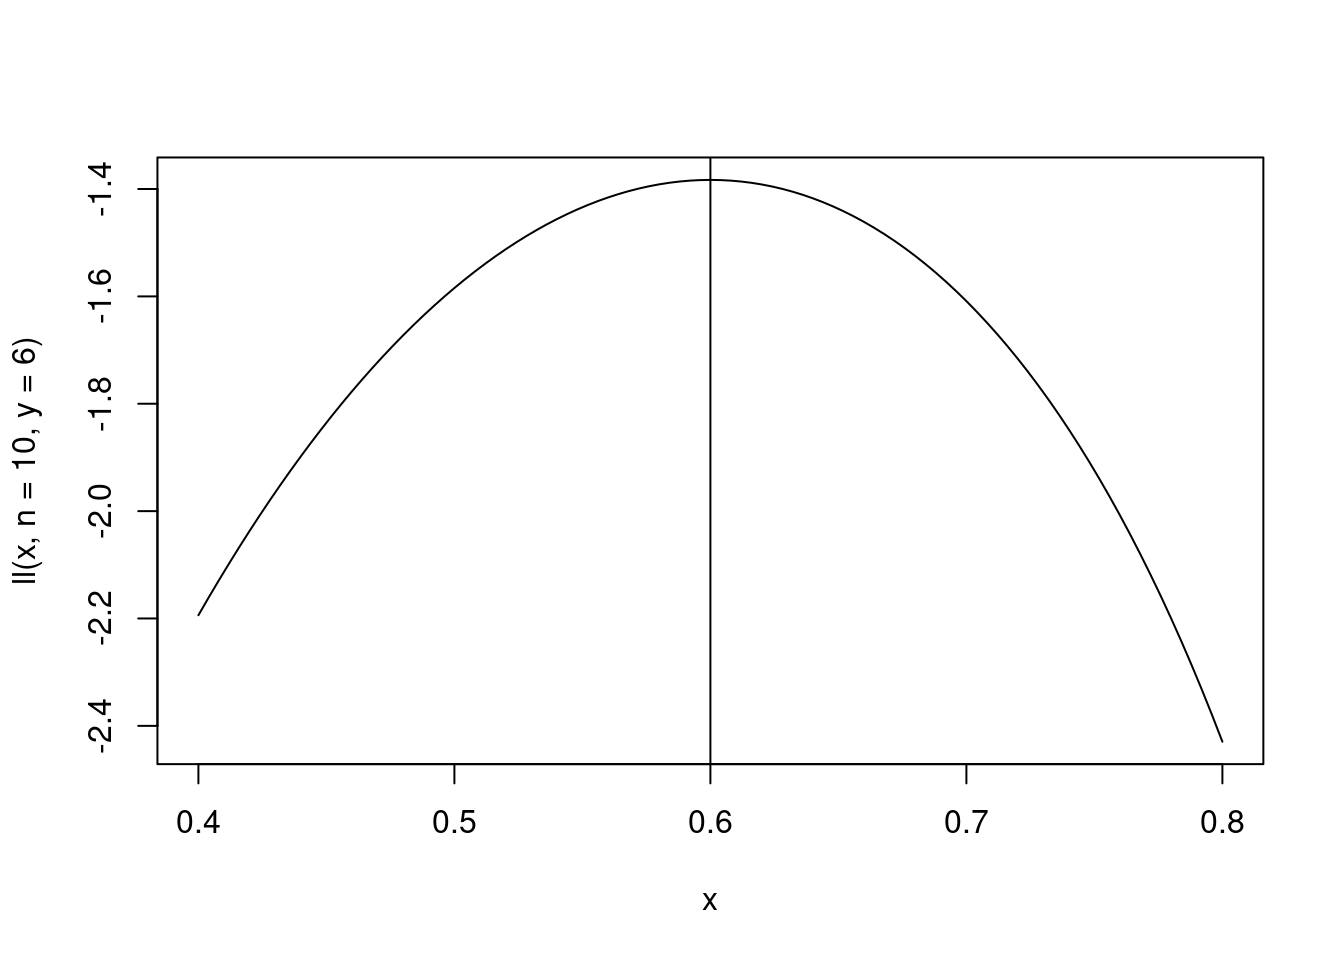
\includegraphics{figures/unnamed-chunk-375-1} \end{center}

Não é dificil mostrar usando ferramentas padrões de cálculo diferencial que o ponto de máximo ocorre em \(\hat{p} = y/n\), ou seja, na proporção amostral de eleitores do candidato X.

Com essa ideia simples resolvemos o primeiro objetivo da inferência estatística que consiste em dizer qual valor achamos razoável para \(p\) dado a amostra que coletamos.
O próximo objetivo é dizer o quanto acreditamos neste valor. Note que uma vez que temos a função de verossimilhança ou log-verossmilhança basta olhar para a função para responder a tal pergunta. O ponto de máximo é o mais compatível, porém valores ao redor do máximo também apresentam uma boa compatibilidade com a amostra e portanto são bons candidatos a valor de \(p\). Essa ideia pode ser resumida por fazer um corte horizontal na função de log-verossimilhança. Assim, todos os pontos acima do corte são bons candidatos a verdadeiro valor de \(p\).

\begin{Shaded}
\begin{Highlighting}[]
\FunctionTok{curve}\NormalTok{(}\FunctionTok{ll}\NormalTok{(x, }\AttributeTok{n =} \DecValTok{10}\NormalTok{, }\AttributeTok{y =} \DecValTok{6}\NormalTok{), }\FloatTok{0.4}\NormalTok{, }\FloatTok{0.8}\NormalTok{)}
\FunctionTok{abline}\NormalTok{(}\AttributeTok{h =} \SpecialCharTok{{-}}\DecValTok{2}\NormalTok{)}
\end{Highlighting}
\end{Shaded}

\begin{center}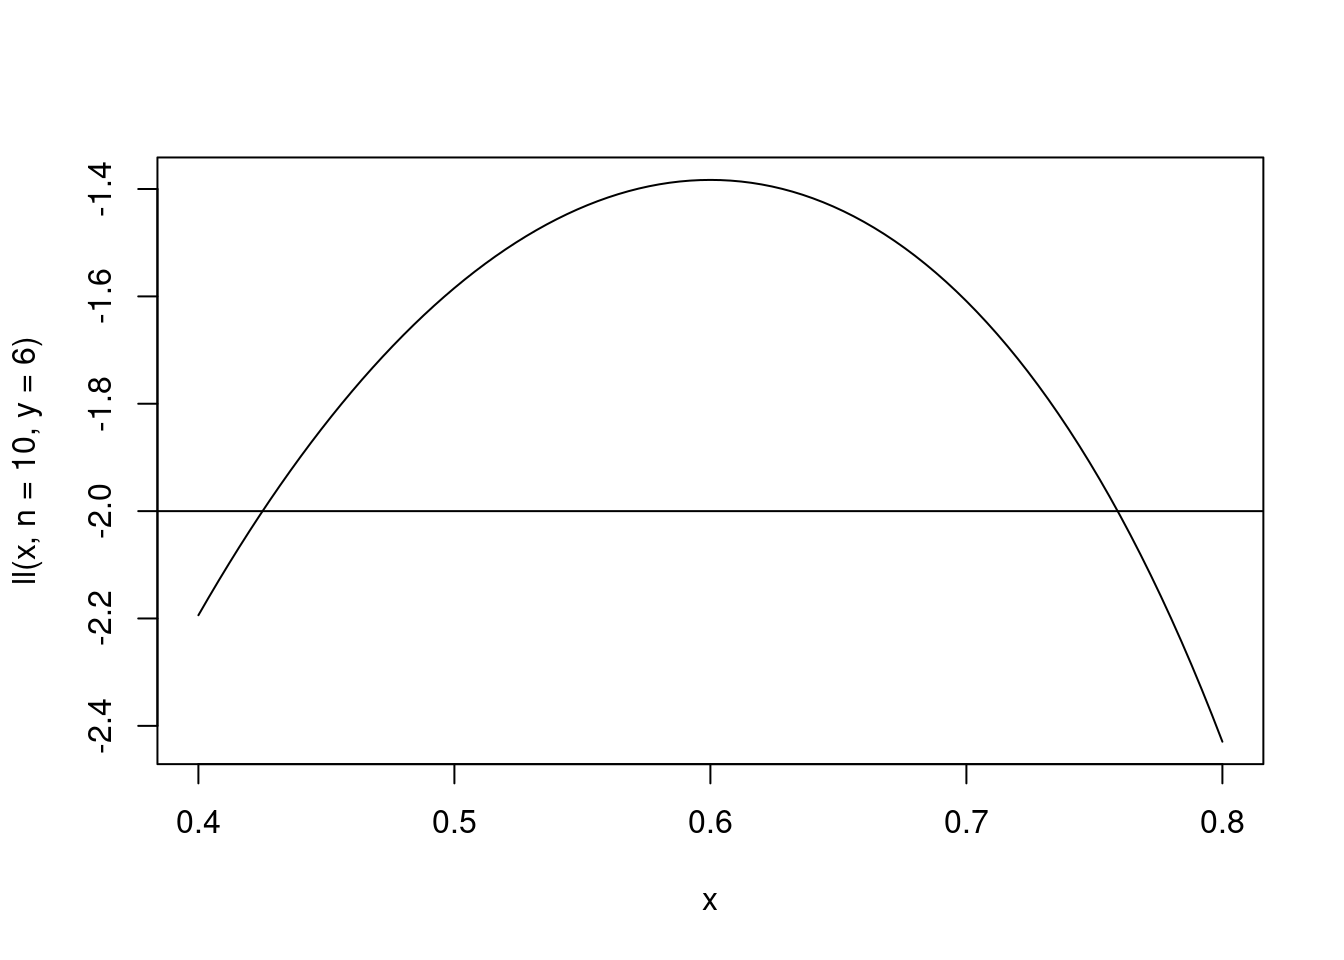
\includegraphics{figures/unnamed-chunk-376-1} \end{center}

Entretanto, onde fazer tal corte não é uma tarefa simples e explicar como e por que fazer isso em detalhes está fora do escopo deste material. Esta é a ideia por traz da definição do que se chama popularmente de intervalo de confiança.
Uma forma alternativa é fazer um gráfico da função de verossimilhança relativa, definida como a verossimilhança divida pela verossimilhança no ponto de máximo,
\[
LR(p) = L(p)/L(\hat{p}).
\]

Neste caso um intervalo pode ser obtido por definir algum valor entre \(0\) e \(1\) para obter intervalos não vazios. Por exemplo, podemos definir que uma compatibilidade de pelo menos 0.4 com a amostra é necessário para que um valor seja parte do intervalo. Ilustrando graficamente temos,

\begin{Shaded}
\begin{Highlighting}[]
\NormalTok{LR }\OtherTok{\textless{}{-}} \ControlFlowTok{function}\NormalTok{(p, p\_hat, n, y) \{}
\NormalTok{  out }\OtherTok{\textless{}{-}} \FunctionTok{L}\NormalTok{(}\AttributeTok{p =}\NormalTok{ p, }\AttributeTok{n =}\NormalTok{ n, }\AttributeTok{y =}\NormalTok{ y)}\SpecialCharTok{/}\FunctionTok{L}\NormalTok{(}\AttributeTok{p =}\NormalTok{ p\_hat, }\AttributeTok{n =}\NormalTok{ n, }\AttributeTok{y =}\NormalTok{ y)}
  \FunctionTok{return}\NormalTok{(out)}
\NormalTok{\}}
\FunctionTok{curve}\NormalTok{(}\FunctionTok{LR}\NormalTok{(x, }\AttributeTok{p\_hat =} \FloatTok{0.6}\NormalTok{, }\AttributeTok{n =} \DecValTok{10}\NormalTok{, }\AttributeTok{y =} \DecValTok{6}\NormalTok{), }\DecValTok{0}\NormalTok{, }\DecValTok{1}\NormalTok{)}
\FunctionTok{abline}\NormalTok{(}\AttributeTok{h =} \FloatTok{0.4}\NormalTok{)}
\end{Highlighting}
\end{Shaded}

\begin{center}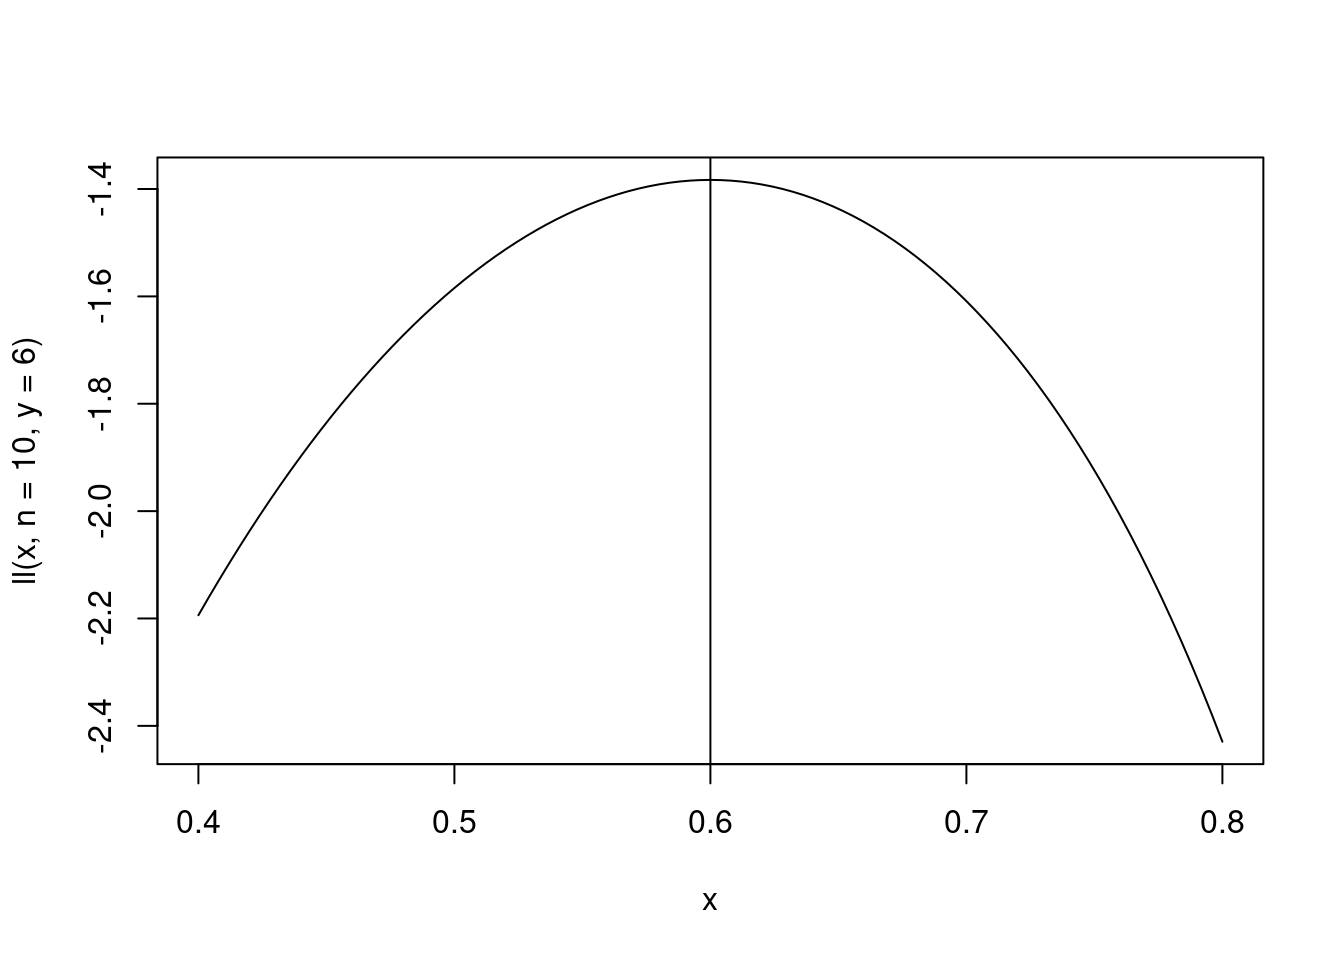
\includegraphics{figures/unnamed-chunk-377-1} \end{center}

Por fim, o último objetivo da inferência consiste em decidir se um determinado valor hipotético para \(p\) é ou não compatível com a amostra observada. Note que o valor mais compatível é o máximo da verossimilhança, assim para decidir se um valor é ou não compatível com a amostra, basta verificar se ele está perto ou longe do valor que tem maior compatibilidade. Esta ideia é o que esta por traz do que se chama de teste de hipóteses e é ilustrada abaixo.

\begin{center}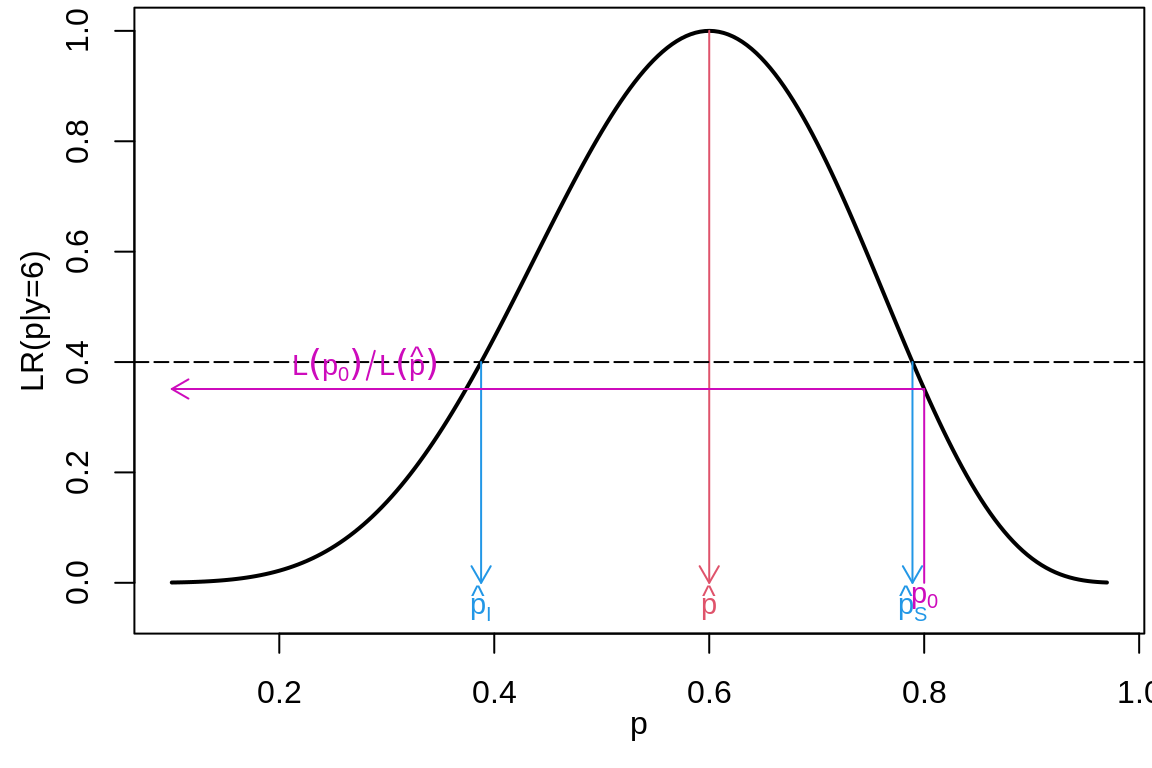
\includegraphics{figures/unnamed-chunk-378-1} \end{center}

\hypertarget{estimauxe7uxe3o-pontual-e-intervalos-de-confianuxe7a}{%
\section{Estimação pontual e intervalos de confiança}\label{estimauxe7uxe3o-pontual-e-intervalos-de-confianuxe7a}}

O processo de estimação pontual consiste em encontrar um valor ao qual chamamos de estimativa do verdadeiro valor do parâmetro, em nosso exemplo o parâmetro \(p\) da distribuição Bernoulli. Como discutido anteriormente a função de verossimilhança nos fornece uma forma intuitiva de obter tal valor que no caso da distribuição de Bernoulli é simplesmente a proporção amostral, \(\hat{p} = y/n\).

O próximo passo é encontrar um intervalo de confiança para o parâmetro \(p\). Neste texto vamos enfatizar o pensamento frequentista de probabilidade para motivar a construção do intervalo de confiança.

Importante salientar que \(Y\) é uma variável aleatória cuja observações são denotadas por \(y\). Nossa estimativa de \(p\) é o valor \(\hat{p} = y/n\) que é uma função dos valores observados. Agora suponha que o experimento seja refeito um número grande vezes. O que vai acontecer com \(\hat{p}\)? Vamos fazer um experimento computacional para ilustrar esta situação.

\begin{Shaded}
\begin{Highlighting}[]
\FunctionTok{set.seed}\NormalTok{(}\DecValTok{1234}\NormalTok{)}
\NormalTok{p.hat }\OtherTok{\textless{}{-}} \FunctionTok{c}\NormalTok{()}
\ControlFlowTok{for}\NormalTok{(i }\ControlFlowTok{in} \DecValTok{1}\SpecialCharTok{:}\DecValTok{1000}\NormalTok{) \{}
\NormalTok{  y }\OtherTok{\textless{}{-}} \FunctionTok{rbinom}\NormalTok{(}\DecValTok{10}\NormalTok{, }\AttributeTok{prob =} \FloatTok{0.5}\NormalTok{, }\AttributeTok{size =} \DecValTok{1}\NormalTok{)}
\NormalTok{  p.hat[i] }\OtherTok{\textless{}{-}} \FunctionTok{mean}\NormalTok{(y)}
\NormalTok{\}}
\end{Highlighting}
\end{Shaded}

\begin{Shaded}
\begin{Highlighting}[]
\FunctionTok{par}\NormalTok{(}\AttributeTok{mfrow =} \FunctionTok{c}\NormalTok{(}\DecValTok{1}\NormalTok{,}\DecValTok{1}\NormalTok{), }\AttributeTok{mar=}\FunctionTok{c}\NormalTok{(}\FloatTok{2.6}\NormalTok{, }\FloatTok{2.8}\NormalTok{, }\FloatTok{1.2}\NormalTok{, }\FloatTok{0.5}\NormalTok{), }\AttributeTok{mgp =} \FunctionTok{c}\NormalTok{(}\FloatTok{1.6}\NormalTok{, }\FloatTok{0.6}\NormalTok{, }\DecValTok{0}\NormalTok{))}
\FunctionTok{plot}\NormalTok{(}\FunctionTok{prop.table}\NormalTok{(}\FunctionTok{table}\NormalTok{(p.hat)), }\AttributeTok{main =} \StringTok{""}\NormalTok{, }
     \AttributeTok{ylab =} \StringTok{"Proporção observada"}\NormalTok{,}
     \AttributeTok{xlab =} \FunctionTok{expression}\NormalTok{(}\FunctionTok{hat}\NormalTok{(p)), }\AttributeTok{xlim =} \FunctionTok{c}\NormalTok{(}\DecValTok{0}\NormalTok{,}\DecValTok{1}\NormalTok{))}
\end{Highlighting}
\end{Shaded}

\begin{center}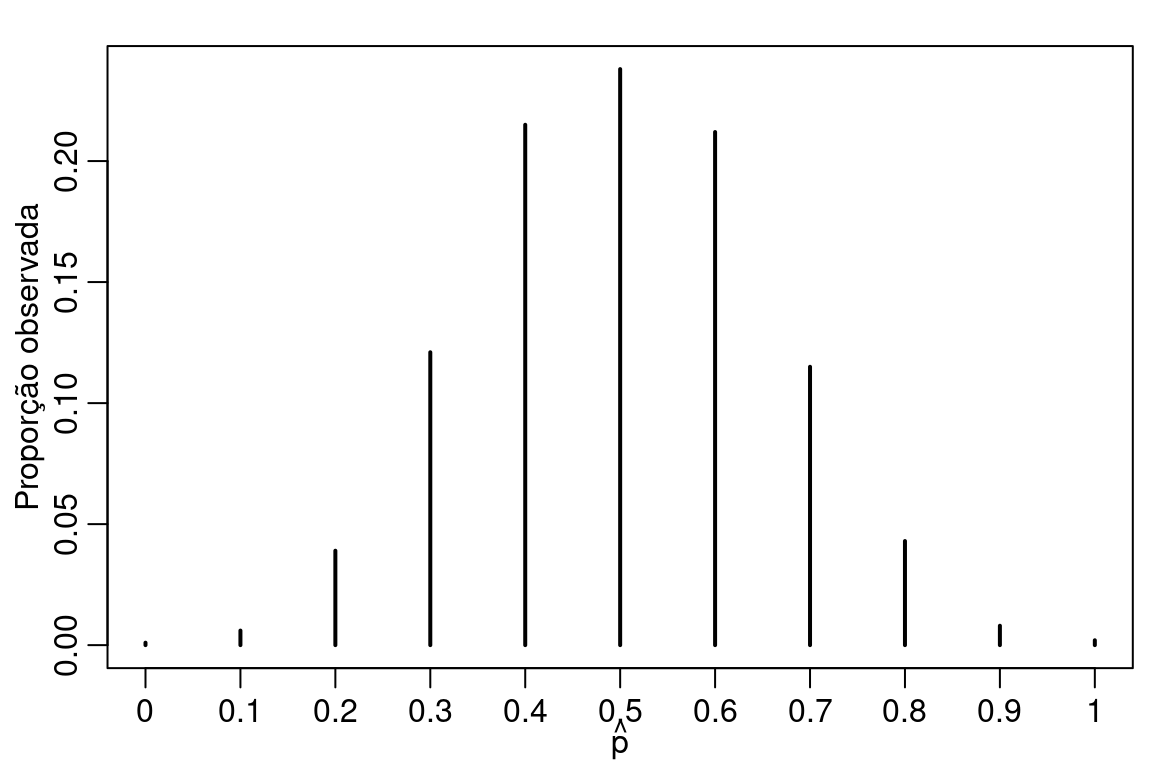
\includegraphics{figures/unnamed-chunk-380-1} \end{center}

A Figura acima mostra que mesmo o verdadeiro valor de \(p\) sendo 0.5 existe uma probabilidade razoável de observarmos \(\hat{p} = 0.4\) e \(\hat{p} = 0.6\) em uma amostra de tamanho 10. Porém, quando nos distanciamos de \(0.5\) a probabilidade de observar \(\hat{p}\) mais extremos como 0.1 ou 0.9 é pequena. No geral, a incerteza com relação ao valor de \(p\) é grande. Para diminuir tal incerteza precisamos ganhar mais informações sobre o valor de \(p\) e para isso precisamos de mais amostras.

Note que para cada possível amostra coletada o valor de \(\hat{p}\) é alterado. Isso é decorrente de \(\hat{p}\) ser também uma função da variável aleatória \(Y\). Para enfatizar isso usamos a notação \(\hat{p} = Y/n\) e neste caso chamamos \(\hat{p}\) de estimador do valor de \(p\). Pensando desta forma \(\hat{p}\) é também uma variável aleatória e consequentemente ele deve ter uma distribuição de probabilidade que pode ser resumida, por exemplo, usando esperança e variância.

A Figura abaixo mostra o efeito do tamanho da amostra sobre a distribuição amostral do estimador \(\hat{p}\).

\begin{Shaded}
\begin{Highlighting}[]
\FunctionTok{set.seed}\NormalTok{(}\DecValTok{1234}\NormalTok{)}
\NormalTok{p.hat.list }\OtherTok{\textless{}{-}} \FunctionTok{list}\NormalTok{()}
\NormalTok{amostra }\OtherTok{\textless{}{-}} \FunctionTok{c}\NormalTok{(}\DecValTok{10}\NormalTok{, }\DecValTok{50}\NormalTok{, }\DecValTok{100}\NormalTok{, }\DecValTok{250}\NormalTok{,}\DecValTok{500}\NormalTok{, }\DecValTok{1000}\NormalTok{)}
\FunctionTok{par}\NormalTok{(}\AttributeTok{mfrow =} \FunctionTok{c}\NormalTok{(}\DecValTok{2}\NormalTok{,}\DecValTok{3}\NormalTok{), }\AttributeTok{mar=}\FunctionTok{c}\NormalTok{(}\FloatTok{2.6}\NormalTok{, }\FloatTok{2.8}\NormalTok{, }\FloatTok{1.2}\NormalTok{, }\FloatTok{0.5}\NormalTok{), }\AttributeTok{mgp =} \FunctionTok{c}\NormalTok{(}\FloatTok{1.6}\NormalTok{, }\FloatTok{0.6}\NormalTok{, }\DecValTok{0}\NormalTok{))}
\ControlFlowTok{for}\NormalTok{(j }\ControlFlowTok{in} \DecValTok{1}\SpecialCharTok{:}\DecValTok{6}\NormalTok{) \{}
\NormalTok{  p.hat.list[[j]] }\OtherTok{\textless{}{-}} \FunctionTok{matrix}\NormalTok{(}\ConstantTok{NA}\NormalTok{, }\AttributeTok{ncol =} \DecValTok{1}\NormalTok{, }\AttributeTok{nrow =} \DecValTok{1000}\NormalTok{)}
  \ControlFlowTok{for}\NormalTok{(i }\ControlFlowTok{in} \DecValTok{1}\SpecialCharTok{:}\DecValTok{1000}\NormalTok{) \{}
\NormalTok{  y }\OtherTok{\textless{}{-}} \FunctionTok{rbinom}\NormalTok{(amostra[j], }\AttributeTok{prob =} \FloatTok{0.5}\NormalTok{, }\AttributeTok{size =} \DecValTok{1}\NormalTok{)}
\NormalTok{  p.hat.list[[j]][i,] }\OtherTok{\textless{}{-}} \FunctionTok{mean}\NormalTok{(y)}
\NormalTok{  \}}
\FunctionTok{hist}\NormalTok{(p.hat.list[[j]], }\AttributeTok{prob =} \ConstantTok{TRUE}\NormalTok{, }\AttributeTok{main =} \FunctionTok{paste}\NormalTok{(}\StringTok{"Amostra"}\NormalTok{, amostra[j]), }
     \AttributeTok{ylab =} \StringTok{"Proporção observada"}\NormalTok{,}
     \AttributeTok{xlab =} \FunctionTok{expression}\NormalTok{(}\FunctionTok{hat}\NormalTok{(p)), }\AttributeTok{xlim =} \FunctionTok{c}\NormalTok{(}\DecValTok{0}\NormalTok{,}\DecValTok{1}\NormalTok{))}
\NormalTok{\}}
\end{Highlighting}
\end{Shaded}

\begin{center}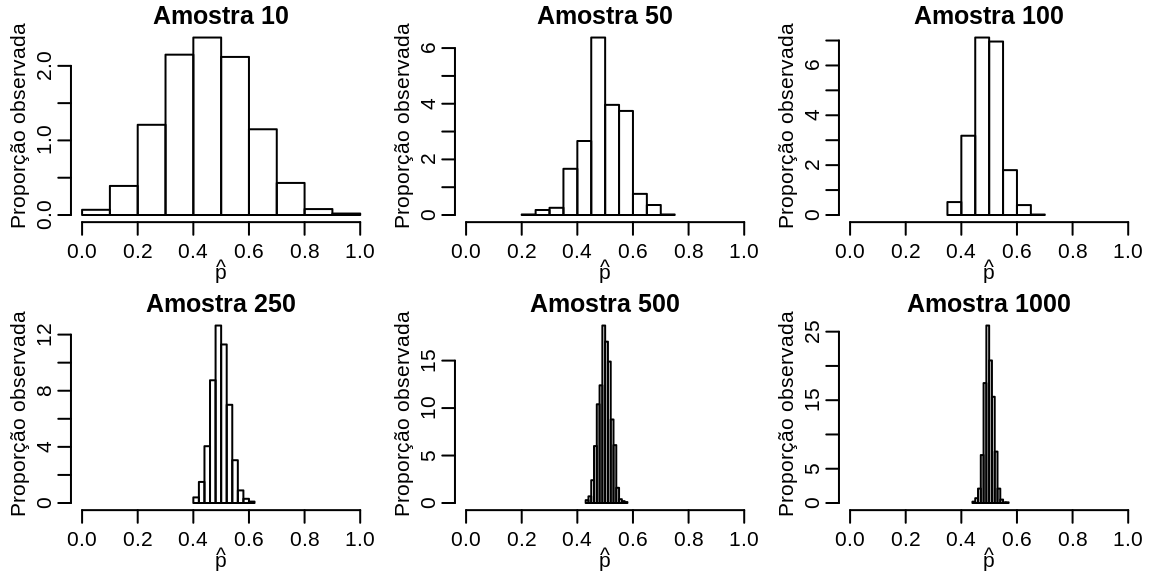
\includegraphics[width=0.99\linewidth]{figures/unnamed-chunk-381-1} \end{center}

Note que quanto maior a amostra a distribuição amostral fica mais concentrada ao redor do verdadeiro valor de \(p\). Isso é decorrente da Lei dos grandes números. Além disso, note que a distribuição é muito parecida com a distribuição normal, um resultado conhecido como Teorema Central do Limite.

A idéia de intervalo de confiança é simplesmente olhar para a distribuição amostral e responder a pergunta: Qual o intervalo em que \(\hat{p}\) tem uma probabilidade, digamos \((1-\alpha)\) de pertencer?

O valor de \(\alpha\) deve ser especificado e alguns valores populares são \(0.05\) e \(0.01\).
A Figura abaixo ilustra esta ideia.

\begin{Shaded}
\begin{Highlighting}[]
\FunctionTok{set.seed}\NormalTok{(}\DecValTok{1234}\NormalTok{)}
\NormalTok{p.hat.list }\OtherTok{\textless{}{-}} \FunctionTok{list}\NormalTok{()}
\NormalTok{amostra }\OtherTok{\textless{}{-}} \FunctionTok{c}\NormalTok{(}\DecValTok{10}\NormalTok{, }\DecValTok{50}\NormalTok{, }\DecValTok{100}\NormalTok{)}
\FunctionTok{par}\NormalTok{(}\AttributeTok{mfrow =} \FunctionTok{c}\NormalTok{(}\DecValTok{1}\NormalTok{,}\DecValTok{3}\NormalTok{), }\AttributeTok{mar=}\FunctionTok{c}\NormalTok{(}\FloatTok{2.6}\NormalTok{, }\FloatTok{2.8}\NormalTok{, }\FloatTok{1.2}\NormalTok{, }\FloatTok{0.5}\NormalTok{), }\AttributeTok{mgp =} \FunctionTok{c}\NormalTok{(}\FloatTok{1.6}\NormalTok{, }\FloatTok{0.6}\NormalTok{, }\DecValTok{0}\NormalTok{))}
\ControlFlowTok{for}\NormalTok{(j }\ControlFlowTok{in} \DecValTok{1}\SpecialCharTok{:}\DecValTok{3}\NormalTok{) \{}
\NormalTok{  p.hat.list[[j]] }\OtherTok{\textless{}{-}} \FunctionTok{matrix}\NormalTok{(}\ConstantTok{NA}\NormalTok{, }\AttributeTok{ncol =} \DecValTok{1}\NormalTok{, }\AttributeTok{nrow =} \DecValTok{1000}\NormalTok{)}
  \ControlFlowTok{for}\NormalTok{(i }\ControlFlowTok{in} \DecValTok{1}\SpecialCharTok{:}\DecValTok{1000}\NormalTok{) \{}
\NormalTok{  y }\OtherTok{\textless{}{-}} \FunctionTok{rbinom}\NormalTok{(amostra[j], }\AttributeTok{prob =} \FloatTok{0.5}\NormalTok{, }\AttributeTok{size =} \DecValTok{1}\NormalTok{)}
\NormalTok{  p.hat.list[[j]][i,] }\OtherTok{\textless{}{-}} \FunctionTok{mean}\NormalTok{(y)}
\NormalTok{  \}}
\FunctionTok{hist}\NormalTok{(p.hat.list[[j]], }\AttributeTok{prob =} \ConstantTok{TRUE}\NormalTok{, }\AttributeTok{main =} \FunctionTok{paste}\NormalTok{(}\StringTok{"Amostra"}\NormalTok{, amostra[j]), }
     \AttributeTok{ylab =} \StringTok{"Densidade"}\NormalTok{,}
     \AttributeTok{xlab =} \FunctionTok{expression}\NormalTok{(}\FunctionTok{hat}\NormalTok{(p)), }\AttributeTok{xlim =} \FunctionTok{c}\NormalTok{(}\DecValTok{0}\NormalTok{,}\DecValTok{1}\NormalTok{))}
\FunctionTok{abline}\NormalTok{(}\AttributeTok{v=} \FunctionTok{c}\NormalTok{(}\FunctionTok{quantile}\NormalTok{(p.hat.list[[j]], }\AttributeTok{probs =} \FunctionTok{c}\NormalTok{(}\FloatTok{0.025}\NormalTok{, }\FloatTok{0.975}\NormalTok{))), }\AttributeTok{col =} \StringTok{"red"}\NormalTok{)}
\NormalTok{\}}
\end{Highlighting}
\end{Shaded}

\begin{center}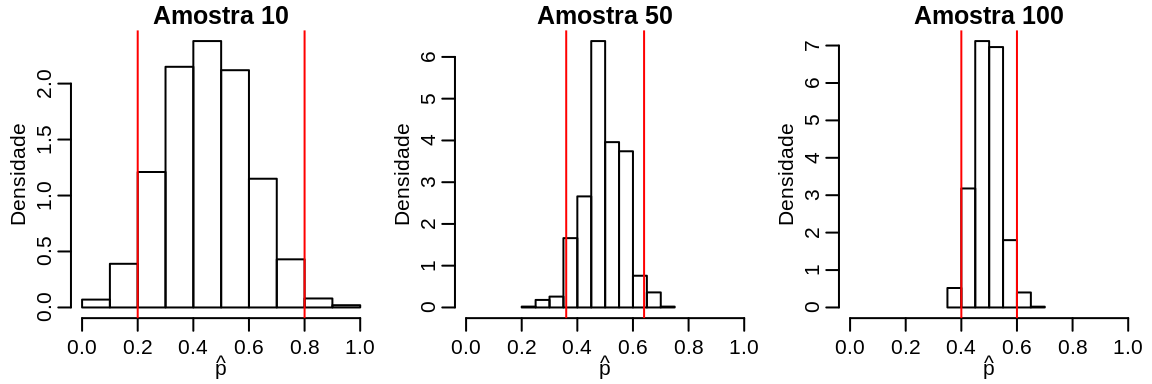
\includegraphics[width=0.99\linewidth]{figures/unnamed-chunk-382-1} \end{center}

Temos um procedimento bastante simples para obter os limites do intervalo de confiança, porém tal procedimento depende de sermos capazes de realizar o experimento um número grande de vezes. Na prática só temos uma amostra coletada e baseado apenas nesta amostra precisamos inferir sobre \(p\). É neste ponto que entra o fato de \(\hat{p}\) ser uma variável aleatória. Este fato permite que exploremos sua distribuição mesmo sem realizar um grande número de experimentos.

De forma geral obter a distribuição de probabilidade de um estimador não é uma tarefa trivial, porém o Teorema Central do Limite nos fornece uma boa aproximação, ao menos para grandes amostras. O Teorema Central do limite em sua versão mais simples é como segue:

\begin{itemize}
\tightlist
\item
  Teorema Lindeberg-Levy: Seja \(Y_1, \ldots, Y_n\) uma amostra iid
  com \(E(Y_i) = \mu\) e \(V(Y_i) = \sigma^2 < \infty\).
  Então,
  \[ \sqrt{n}\left ( \frac{\bar{Y} - \mu}{\sigma} \right ) \overset{D}{\to} Z \sim N(0,1), \quad \text{para} \quad n \to \infty.\]
\item
  Isso significa que, para todo \(y \in \Re\),
  \[ P(Y_n \leq y) \to \Phi (y) \quad \text{quando} \quad n \to \infty,\] onde
  \[ \Phi(y) = \int_{-\infty}^y \phi(z) dz \quad \text{e} \quad 
  \phi(z) = \frac{1}{\sqrt{2\pi}} \exp \left ( -\frac{1}{2} z^2 \right ).\]
\item
  Forma alternativa: \(\bar{Y} \sim N(\mu, \sigma^2/n).\)
\end{itemize}

Particularizando para o nosso exemplo temos que:

\begin{itemize}
\tightlist
\item
  Estimador de máxima verossimilhança \(\hat{p} = \frac{Y}{n}.\)
\item
  Usando as propriedades da distribuição binomial, temos
  \[E(\hat{p}) = E(Y/n) = \frac{1}{n}E(Y) = \frac{np}{n} = p.\]
  \[Var(\hat{p}) = Var(Y/n) = \frac{1}{n^2}Var(Y) = \frac{np(1-p)}{n^2} = \frac{p(1-p)}{n}.\]
\item
  Usando o TLC, temos
  \[\hat{p} \sim N(p, \frac{p(1-p)}{n}).\]
\end{itemize}

Vamos fazer uma ilustração computacional deste importante resultado.

\begin{Shaded}
\begin{Highlighting}[]
\FunctionTok{set.seed}\NormalTok{(}\DecValTok{1234}\NormalTok{)}
\NormalTok{p.hat.list }\OtherTok{\textless{}{-}} \FunctionTok{list}\NormalTok{()}
\NormalTok{amostra }\OtherTok{\textless{}{-}} \FunctionTok{c}\NormalTok{(}\DecValTok{10}\NormalTok{, }\DecValTok{50}\NormalTok{, }\DecValTok{100}\NormalTok{, }\DecValTok{250}\NormalTok{, }\DecValTok{500}\NormalTok{, }\DecValTok{1000}\NormalTok{)}
\FunctionTok{par}\NormalTok{(}\AttributeTok{mfrow =} \FunctionTok{c}\NormalTok{(}\DecValTok{2}\NormalTok{,}\DecValTok{3}\NormalTok{), }\AttributeTok{mar=}\FunctionTok{c}\NormalTok{(}\FloatTok{2.6}\NormalTok{, }\FloatTok{2.8}\NormalTok{, }\FloatTok{1.2}\NormalTok{, }\FloatTok{0.5}\NormalTok{), }\AttributeTok{mgp =} \FunctionTok{c}\NormalTok{(}\FloatTok{1.6}\NormalTok{, }\FloatTok{0.6}\NormalTok{, }\DecValTok{0}\NormalTok{))}
\ControlFlowTok{for}\NormalTok{(j }\ControlFlowTok{in} \DecValTok{1}\SpecialCharTok{:}\DecValTok{6}\NormalTok{) \{}
\NormalTok{  p.hat.list[[j]] }\OtherTok{\textless{}{-}} \FunctionTok{matrix}\NormalTok{(}\ConstantTok{NA}\NormalTok{, }\AttributeTok{ncol =} \DecValTok{1}\NormalTok{, }\AttributeTok{nrow =} \DecValTok{1000}\NormalTok{)}
  \ControlFlowTok{for}\NormalTok{(i }\ControlFlowTok{in} \DecValTok{1}\SpecialCharTok{:}\DecValTok{1000}\NormalTok{) \{}
\NormalTok{  y }\OtherTok{\textless{}{-}} \FunctionTok{rbinom}\NormalTok{(amostra[j], }\AttributeTok{prob =} \FloatTok{0.5}\NormalTok{, }\AttributeTok{size =} \DecValTok{1}\NormalTok{)}
\NormalTok{  p.hat.list[[j]][i,] }\OtherTok{\textless{}{-}} \FunctionTok{mean}\NormalTok{(y)}
\NormalTok{  \}}
  \FunctionTok{hist}\NormalTok{(p.hat.list[[j]], }\AttributeTok{prob =} \ConstantTok{TRUE}\NormalTok{, }\AttributeTok{main =} \FunctionTok{paste}\NormalTok{(}\StringTok{"Amostra"}\NormalTok{, amostra[j]), }
       \AttributeTok{ylab =} \StringTok{"Densidade"}\NormalTok{, }\AttributeTok{xlab =} \FunctionTok{expression}\NormalTok{(}\FunctionTok{hat}\NormalTok{(p)), }\AttributeTok{xlim =} \FunctionTok{c}\NormalTok{(}\DecValTok{0}\NormalTok{,}\DecValTok{1}\NormalTok{))}
  \FunctionTok{curve}\NormalTok{(}\FunctionTok{dnorm}\NormalTok{(x, }\AttributeTok{mean =} \FloatTok{0.5}\NormalTok{, }\AttributeTok{sd =} \FunctionTok{sqrt}\NormalTok{(}\FloatTok{0.5}\SpecialCharTok{*}\NormalTok{(}\DecValTok{1}\FloatTok{{-}0.5}\NormalTok{)}\SpecialCharTok{/}\NormalTok{amostra[j])), }\FloatTok{0.1}\NormalTok{, }\FloatTok{0.9}\NormalTok{, }\AttributeTok{add =} \ConstantTok{TRUE}\NormalTok{)}
\NormalTok{\}}
\end{Highlighting}
\end{Shaded}

\begin{center}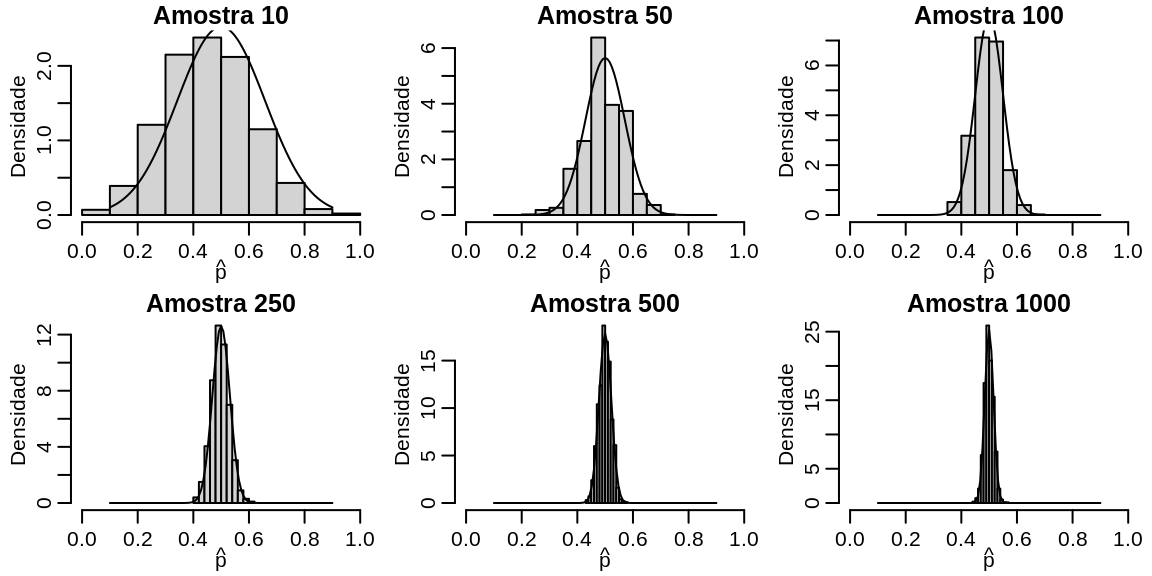
\includegraphics[width=0.99\linewidth]{figures/unnamed-chunk-383-1} \end{center}

Agora usando resultados convencionais da distribuição normal podemos encontrar os limites do intervalo de confiança. Para o caso binomial o intervalo é dado por
\[\hat{p} \pm Z_{\alpha/2} \sqrt{\frac{\hat{p}(1-\hat{p})}{n}},\]
onde \(Z_{\alpha/2}\) é o quantil da distribuição normal padrão com \(\alpha/2\) probabilidade.

Cálculos similares mostram que para os casos da média de uma distribuição normal e Poisson os intervalos ficam dados por:

\begin{itemize}
\item
  Intervalo de confiança: Caso Normal
  \[\hat{\mu} \pm Z_{\alpha/2} \sqrt{\frac{\hat{\sigma}^2}{n}},\]
  onde \(\hat{\sigma}^2 = \sum_{i=1}^n \frac{(y_i - \hat{\mu})^2}{n-1}\).
\item
  Intervalo de confiança: Caso Poisson
  \[\hat{\lambda} \pm Z_{\alpha/2} \sqrt{\frac{\hat{\lambda}}{n}},\]
  onde \(\hat{\lambda} = \sum_{i=1}^n \frac{y_i}{n}.\)
\end{itemize}

O intervalo de confiança deve ser interpretado sempre com muito cuidado. A interpretação frequentista é a seguinte: Se o experimento for repetido um número \(n\) de vezes e para cada realização obtermos o intervalo de confiança, esperamos que \((1-\alpha)\%\) dos intervalos contenham o verdadeiro valor do parâmetro. Note que a variável aleatória é o próprio intervalo de confiança.

O código abaixo ilustra computacionalmente tal interpretação.

\begin{Shaded}
\begin{Highlighting}[]
\FunctionTok{set.seed}\NormalTok{(}\DecValTok{12}\NormalTok{)}
\NormalTok{results\_wald }\OtherTok{\textless{}{-}} \FunctionTok{matrix}\NormalTok{(}\ConstantTok{NA}\NormalTok{, }\AttributeTok{ncol =} \DecValTok{2}\NormalTok{, }\AttributeTok{nrow =} \DecValTok{100}\NormalTok{)}
\ControlFlowTok{for}\NormalTok{(i }\ControlFlowTok{in} \DecValTok{1}\SpecialCharTok{:}\DecValTok{100}\NormalTok{) \{}
\NormalTok{  y }\OtherTok{\textless{}{-}} \FunctionTok{rbinom}\NormalTok{(}\DecValTok{100}\NormalTok{, }\AttributeTok{size =} \DecValTok{1}\NormalTok{, }\AttributeTok{prob =} \FloatTok{0.5}\NormalTok{)}
\NormalTok{  p\_hat }\OtherTok{\textless{}{-}} \FunctionTok{mean}\NormalTok{(y)}
\NormalTok{  v\_hat }\OtherTok{\textless{}{-}}\NormalTok{ (p\_hat}\SpecialCharTok{*}\NormalTok{(}\DecValTok{1}\SpecialCharTok{{-}}\NormalTok{p\_hat))}\SpecialCharTok{/}\DecValTok{100}
\NormalTok{  temp\_wald }\OtherTok{\textless{}{-}} \FunctionTok{c}\NormalTok{(p\_hat }\SpecialCharTok{{-}}  \FunctionTok{qnorm}\NormalTok{(}\FloatTok{0.975}\NormalTok{)}\SpecialCharTok{*}\FunctionTok{sqrt}\NormalTok{(v\_hat), p\_hat }\SpecialCharTok{+} \FunctionTok{qnorm}\NormalTok{(}\FloatTok{0.975}\NormalTok{)}\SpecialCharTok{*}\FunctionTok{sqrt}\NormalTok{(v\_hat))}
\NormalTok{  results\_wald[i,] }\OtherTok{\textless{}{-}}\NormalTok{ temp\_wald}
\NormalTok{\}}

\DocumentationTok{\#\# Intervalo Wald}
\FunctionTok{plot}\NormalTok{(}\FunctionTok{c}\NormalTok{(}\FloatTok{0.30}\NormalTok{,}\FloatTok{0.72}\NormalTok{) }\SpecialCharTok{\textasciitilde{}} \FunctionTok{c}\NormalTok{(}\DecValTok{1}\NormalTok{,}\DecValTok{100}\NormalTok{), }\AttributeTok{type =} \StringTok{"n"}\NormalTok{, }\AttributeTok{ylab =} \FunctionTok{expression}\NormalTok{(p), }\AttributeTok{xlab =} \StringTok{"Ensaio"}\NormalTok{)}
\FunctionTok{abline}\NormalTok{(}\AttributeTok{h=}\FloatTok{0.50}\NormalTok{)}
\ControlFlowTok{for}\NormalTok{(i }\ControlFlowTok{in} \DecValTok{1}\SpecialCharTok{:}\DecValTok{100}\NormalTok{) \{}
  \FunctionTok{arrows}\NormalTok{(}\FunctionTok{c}\NormalTok{(i),results\_wald[i,}\DecValTok{1}\NormalTok{],}\FunctionTok{c}\NormalTok{(i),results\_wald[i,}\DecValTok{2}\NormalTok{],}\AttributeTok{code=}\DecValTok{3}\NormalTok{,}\AttributeTok{angle=}\DecValTok{90}\NormalTok{,}\AttributeTok{length=}\FloatTok{0.03}\NormalTok{,}
         \AttributeTok{col=}\FunctionTok{ifelse}\NormalTok{(results\_wald[i,}\DecValTok{1}\NormalTok{] }\SpecialCharTok{\textgreater{}} \FloatTok{0.5} \SpecialCharTok{|}\NormalTok{ results\_wald[i,}\DecValTok{2}\NormalTok{] }\SpecialCharTok{\textless{}} \FloatTok{0.5}\NormalTok{, }\StringTok{"darkred"}\NormalTok{,}\StringTok{"lightgray"}\NormalTok{))}
\NormalTok{\}}
\end{Highlighting}
\end{Shaded}

\begin{center}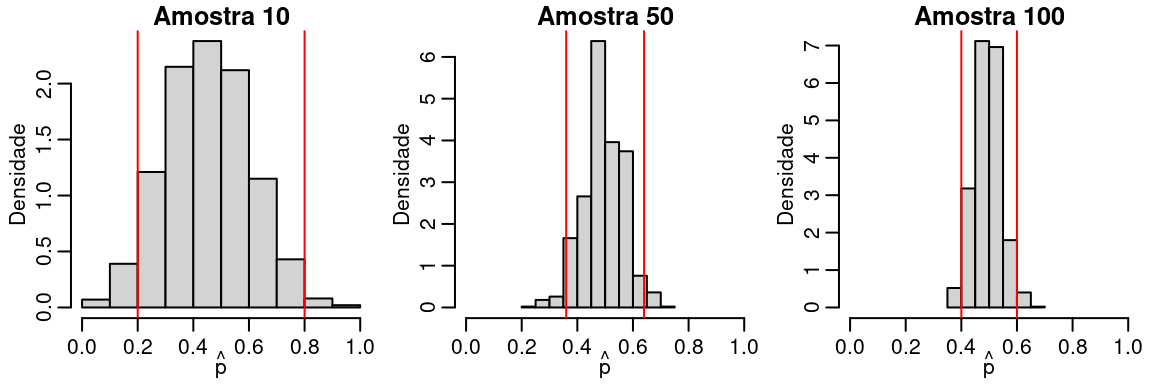
\includegraphics{figures/unnamed-chunk-384-1} \end{center}

\textbf{Exemplo 1} No caso do candidato X suponha que é de interesse apresentar uma estimativa intervalar para a proporção de eleitores de X na população. Assumindo que a estimativa amostral foi de \(0,60\) (seis sucessos em dez ensaios) o intervalo com \(95\%\) de confiança é dado por
\[
\hat{p}_I = 0,6 - 1.96\sqrt{0,6(1-0,6)/10} = 0.296 \quad \text{e} \quad \hat{p}_S = 0,6 - 1.96\sqrt{0,6(1-0,6)/10} = 0.904.
\]

\textbf{Exemplo 2} Num grupo de pacientes, o nível de colesterol é uma variável aleatória com distribuição Normal, de média desconhecida e variância \(64 (mg/ml)^2\).
- Para uma amostra de 46 indivíduos que forneceu nível médio de colesterol de 120 \(mg/ml\), construa o intervalo de confiança de \(88\%\).

\begin{Shaded}
\begin{Highlighting}[]
\NormalTok{media }\OtherTok{\textless{}{-}} \DecValTok{120}
\NormalTok{sd }\OtherTok{\textless{}{-}} \FunctionTok{sqrt}\NormalTok{(}\DecValTok{64}\NormalTok{)}
\NormalTok{n }\OtherTok{\textless{}{-}} \DecValTok{46}
\NormalTok{alpha }\OtherTok{=} \FloatTok{0.12}
\NormalTok{mu\_I }\OtherTok{\textless{}{-}}\NormalTok{ media }\SpecialCharTok{{-}} \FunctionTok{qnorm}\NormalTok{((}\DecValTok{1} \SpecialCharTok{{-}}\NormalTok{ alpha}\SpecialCharTok{/}\DecValTok{2}\NormalTok{))}\SpecialCharTok{*}\NormalTok{sd}\SpecialCharTok{/}\FunctionTok{sqrt}\NormalTok{(}\DecValTok{46}\NormalTok{)}
\NormalTok{mu\_S }\OtherTok{\textless{}{-}}\NormalTok{ media }\SpecialCharTok{+} \FunctionTok{qnorm}\NormalTok{((}\DecValTok{1} \SpecialCharTok{{-}}\NormalTok{ alpha}\SpecialCharTok{/}\DecValTok{2}\NormalTok{))}\SpecialCharTok{*}\NormalTok{sd}\SpecialCharTok{/}\FunctionTok{sqrt}\NormalTok{(}\DecValTok{46}\NormalTok{)}
\FunctionTok{c}\NormalTok{(mu\_I, mu\_S)}
\NormalTok{[}\DecValTok{1}\NormalTok{] }\FloatTok{118.1661} \FloatTok{121.8339}
\end{Highlighting}
\end{Shaded}

\hypertarget{exercuxedcios-18}{%
\section*{Exercícios}\label{exercuxedcios-18}}


\begin{enumerate}
\def\labelenumi{\arabic{enumi}.}
\item
  Por analogia a produtos similares, o tempo de reação de um novo medicamento pode ser considerado como tendo distribuição Normal com desvio padrão igual a 2 minutos (a média desconhecida). Vinte pacientes foram sorteados, receberam o medicamento e tiveram seu tempo de reação anotado. Os dados foram os seguintes (em minutos): \(2,9; 3,4; 3,5; 4,1; 4,6; 4,7; 4,5; 3,8; 5,3; 4,9; 4,8; 5,7; 5,8; 5,0; 3,4; 5,9; 6,3; 4,6; 5,5\) e \(6,2\). Obtenha um intervalo de confiança para o tempo médio de reação. Use \(96\%\) de confiança.
\item
  Uma amostra de 25 observações de uma Normal \((\mu, 16)\) foi coletada e forneceu uma média amostral de 8. Construa intervalos de confiança com \(80\%\), \(85\%\), \(90\%\) e \(95\%\) de confiança. Comente as diferenças encontradas.
\item
  Numa pesquisa com 50 eleitores, o candidato José João obteve \(0,34\) da preferência dos eleitores. Construa, para a confiança de \(94\%\) o intervalo de confiança para a proporção de votos a serem recebidos pelo candidato mencionado.
\item
  Considere a seguinte amostra da distribuição de Poisson de parâmetro \(\lambda\). Proponha um estimador pontual e intervalar para \(\lambda\) usando o método de máxima verossimilhança. Implemente seu método em R. Faça um estudo de simulação para ilustrar a distribuição aproximada deste estimador.
\item
  O número de atendimentos em um pronto-socorro pode ser modelado por uma distribuição de Poisson de parâmetro \(\lambda\). Suponha que o interesse seja modelar o número de atendimentos por hora e que para um conjunto de \(30\) horas o número de atendimentos por hora foi contado e as observações são mostradas abaixo.
\end{enumerate}

\begin{verbatim}
# A tibble: 3 x 1
  `matrix(y, 3, 10)`[,1]  [,2]  [,3]  [,4]  [,5]  [,6]  [,7]  [,8]  [,9] [,10]
                   <int> <int> <int> <int> <int> <int> <int> <int> <int> <int>
1                      6    11     8     8     9    12     7     9     9     9
2                     10    13    12    13     8     6    13     9     9     6
3                      7     4     8     8     5     3    12    16     8     5
\end{verbatim}

O seu interesse é dimensionar o número de médicos para este pronto socorro.
Suponha que um médico consegue atender até quatro pessoas em um período de uma hora. A politica do hospital especifica que se deve manter um contigente de médicos necessários para atender a demanda em \(95\%\) dos dias. Especifique quantos médicos devem estar de plantão para que a politica do hospital seja respeitada.

\hypertarget{teste-de-hipuxf3tese}{%
\section{Teste de hipótese}\label{teste-de-hipuxf3tese}}

O último objetivo da inferência estatística é a construção de testes de hipóteses.
Uma hipótese é qualquer afirmativa sobre uma propriedade da população.
Um teste de hipótese é um procedimento para avaliar uma afirmativa sobre uma propriedade da população. Em termos estatísticos uma hipótese estatística é qualquer afirmativa sobre um parâmetro da distribuição de probabilidade.

Voltando ao nosso exemplo do candidato X, podemos estar interessados por exemplo em saber se a proporção de votos no candidato X é maior que 0.5, o que implicaria que ele ganharia a eleição. Em termos de distribuição de probabilidade essa é uma afirmativa acerca do valor do parâmetro \(p\). Sendo assim, enunciamos as hipóteses da seguinte forma:

\[H_0: p = \frac{1}{2} \quad vs \quad H_1: p \neq \frac{1}{2}.\]
Nesta notação \(H_0\) é chamada de hipótese nula. Por outro lado, \(H_1\) é chamada de hipótese alternativa.

Para construir um teste de hipótese usamos novamente o pensamento frequentista de probabilidade, ou seja, considere que é possível realizar o experimento um número indefinido de vezes. Para cada uma destas realizações obtemos uma estimativa para o valor de \(p\) digamos \(\hat{p}\). Verique quais valores realizados de \(\hat{p}\) são \textbf{razoáveis} de ocorrer sob a hipótese nula. No caso da hipótese nula ser verdadeira podemos facilmente gerar dados do fenômeno de interesse. Neste caso, vamos realizar o experimento \(1000\) vezes e ver como se comporta nosso estimador.

\begin{Shaded}
\begin{Highlighting}[]
\FunctionTok{set.seed}\NormalTok{(}\DecValTok{1234}\NormalTok{)}
\NormalTok{p.hat }\OtherTok{\textless{}{-}} \FunctionTok{c}\NormalTok{()}
\ControlFlowTok{for}\NormalTok{(i }\ControlFlowTok{in} \DecValTok{1}\SpecialCharTok{:}\DecValTok{1000}\NormalTok{) \{}
\NormalTok{  y }\OtherTok{\textless{}{-}} \FunctionTok{rbinom}\NormalTok{(}\DecValTok{10}\NormalTok{, }\AttributeTok{prob =} \FloatTok{0.5}\NormalTok{, }\AttributeTok{size =} \DecValTok{1}\NormalTok{)}
\NormalTok{  p.hat[i] }\OtherTok{\textless{}{-}} \FunctionTok{mean}\NormalTok{(y)}
\NormalTok{\}}
\FunctionTok{par}\NormalTok{(}\AttributeTok{mfrow =} \FunctionTok{c}\NormalTok{(}\DecValTok{1}\NormalTok{,}\DecValTok{1}\NormalTok{), }\AttributeTok{mar=}\FunctionTok{c}\NormalTok{(}\FloatTok{2.6}\NormalTok{, }\FloatTok{2.8}\NormalTok{, }\FloatTok{1.2}\NormalTok{, }\FloatTok{0.5}\NormalTok{), }\AttributeTok{mgp =} \FunctionTok{c}\NormalTok{(}\FloatTok{1.6}\NormalTok{, }\FloatTok{0.6}\NormalTok{, }\DecValTok{0}\NormalTok{))}
\FunctionTok{plot}\NormalTok{(}\FunctionTok{prop.table}\NormalTok{(}\FunctionTok{table}\NormalTok{(p.hat)), }\AttributeTok{main =} \StringTok{""}\NormalTok{, }
     \AttributeTok{ylab =} \StringTok{"Proporção observada"}\NormalTok{,}
     \AttributeTok{xlab =} \FunctionTok{expression}\NormalTok{(}\FunctionTok{hat}\NormalTok{(p)), }\AttributeTok{xlim =} \FunctionTok{c}\NormalTok{(}\DecValTok{0}\NormalTok{,}\DecValTok{1}\NormalTok{))}
\end{Highlighting}
\end{Shaded}

\begin{center}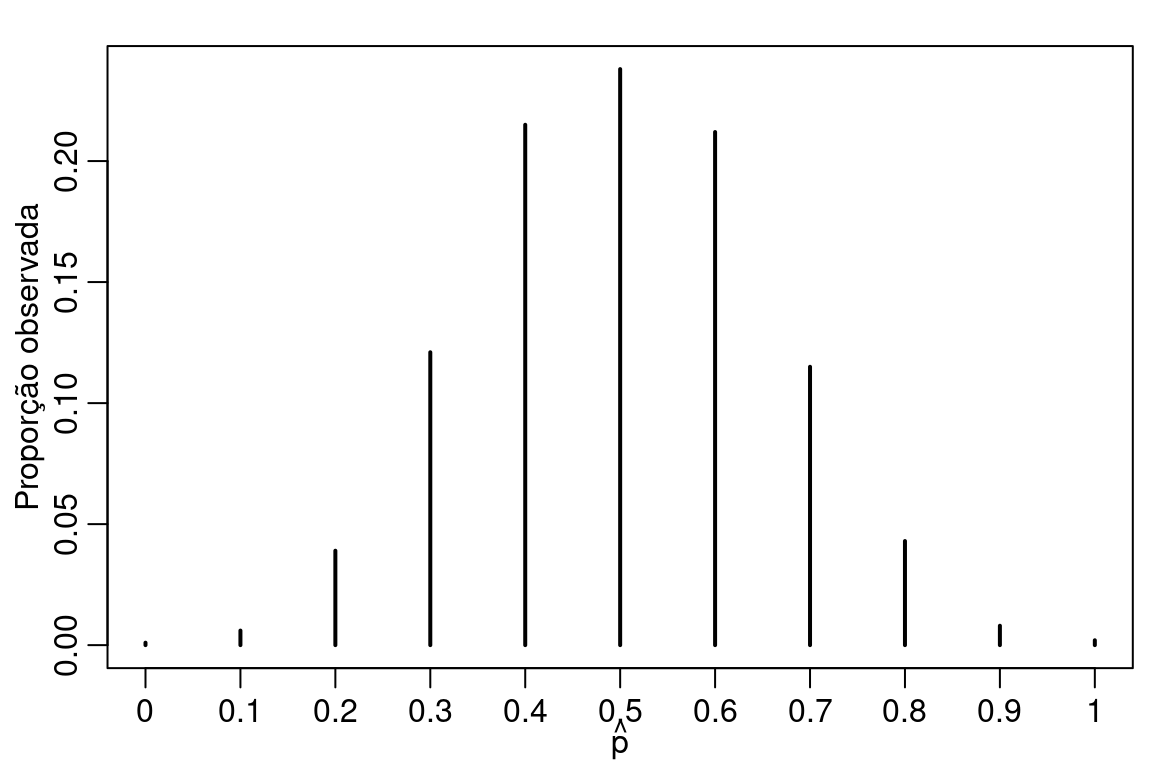
\includegraphics{figures/unnamed-chunk-387-1} \end{center}

Veja que mesmo a hipótese nula sendo verdadeira existe uma probabilidade
não desprezível de observarmos \(8\) eleitores de X em \(10\) eleitores.
A incerteza associada a decisão no caso de apenas \(10\) observações é
grande. Para diminuir a incerteza precisamos de mais informação o que conseguimos aumentanto a amostra. A Figura abaixo ilustra esta situação

\begin{Shaded}
\begin{Highlighting}[]
\FunctionTok{set.seed}\NormalTok{(}\DecValTok{1234}\NormalTok{)}
\NormalTok{p.hat.list }\OtherTok{\textless{}{-}} \FunctionTok{list}\NormalTok{()}
\NormalTok{amostra }\OtherTok{\textless{}{-}} \FunctionTok{c}\NormalTok{(}\DecValTok{10}\NormalTok{, }\DecValTok{50}\NormalTok{, }\DecValTok{100}\NormalTok{, }\DecValTok{250}\NormalTok{,}\DecValTok{500}\NormalTok{)}
\FunctionTok{par}\NormalTok{(}\AttributeTok{mfrow =} \FunctionTok{c}\NormalTok{(}\DecValTok{1}\NormalTok{,}\DecValTok{5}\NormalTok{), }\AttributeTok{mar=}\FunctionTok{c}\NormalTok{(}\FloatTok{2.6}\NormalTok{, }\FloatTok{2.8}\NormalTok{, }\FloatTok{1.2}\NormalTok{, }\FloatTok{0.5}\NormalTok{), }\AttributeTok{mgp =} \FunctionTok{c}\NormalTok{(}\FloatTok{1.6}\NormalTok{, }\FloatTok{0.6}\NormalTok{, }\DecValTok{0}\NormalTok{))}
\ControlFlowTok{for}\NormalTok{(j }\ControlFlowTok{in} \DecValTok{1}\SpecialCharTok{:}\DecValTok{5}\NormalTok{) \{}
\NormalTok{  p.hat.list[[j]] }\OtherTok{\textless{}{-}} \FunctionTok{matrix}\NormalTok{(}\ConstantTok{NA}\NormalTok{, }\AttributeTok{ncol =} \DecValTok{1}\NormalTok{, }\AttributeTok{nrow =} \DecValTok{1000}\NormalTok{)}
  \ControlFlowTok{for}\NormalTok{(i }\ControlFlowTok{in} \DecValTok{1}\SpecialCharTok{:}\DecValTok{1000}\NormalTok{) \{}
\NormalTok{  y }\OtherTok{\textless{}{-}} \FunctionTok{rbinom}\NormalTok{(amostra[j], }\AttributeTok{prob =} \FloatTok{0.5}\NormalTok{, }\AttributeTok{size =} \DecValTok{1}\NormalTok{)}
\NormalTok{  p.hat.list[[j]][i,] }\OtherTok{\textless{}{-}} \FunctionTok{mean}\NormalTok{(y)}
\NormalTok{  \}}
\FunctionTok{hist}\NormalTok{(p.hat.list[[j]], }\AttributeTok{prob =} \ConstantTok{TRUE}\NormalTok{, }\AttributeTok{main =} \FunctionTok{paste}\NormalTok{(}\StringTok{"Amostra"}\NormalTok{, amostra[j]), }
     \AttributeTok{ylab =} \StringTok{"Proporção observada"}\NormalTok{,}
     \AttributeTok{xlab =} \FunctionTok{expression}\NormalTok{(}\FunctionTok{hat}\NormalTok{(p)), }\AttributeTok{xlim =} \FunctionTok{c}\NormalTok{(}\DecValTok{0}\NormalTok{,}\DecValTok{1}\NormalTok{))}
\NormalTok{\}}
\end{Highlighting}
\end{Shaded}

\begin{center}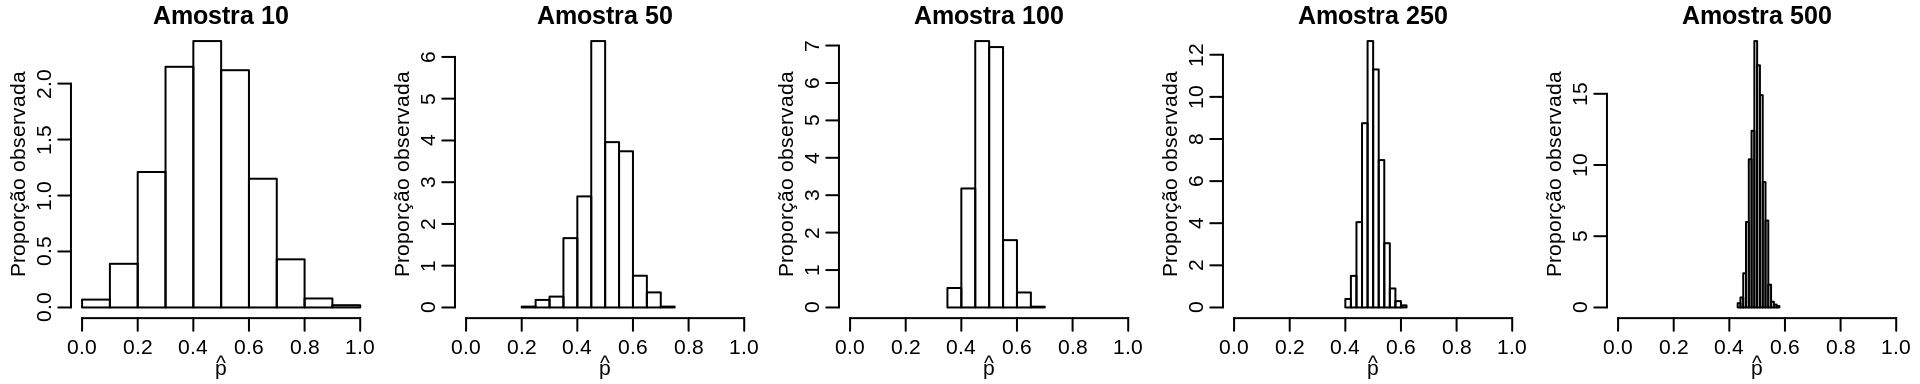
\includegraphics[width=0.99\linewidth]{figures/unnamed-chunk-388-1} \end{center}

O procedimento é bastante intuivo e parecido com a construção de intervalos de confiança. No entanto, no caso de teste de hipóteses precisamos tomar uma decisão. Sendo assim, a ideia é construir uma região de valores para os quais você aceitará (ou não rejeitará) a hipótese nula esta região é chamada de região de aceitação ou não rejeição de \(H_0\).
A Figura abaixo ilustra a construção da região de rejeição

\begin{Shaded}
\begin{Highlighting}[]
\FunctionTok{set.seed}\NormalTok{(}\DecValTok{1234}\NormalTok{)}
\NormalTok{p.hat.list }\OtherTok{\textless{}{-}} \FunctionTok{list}\NormalTok{()}
\NormalTok{amostra }\OtherTok{\textless{}{-}} \FunctionTok{c}\NormalTok{(}\DecValTok{10}\NormalTok{, }\DecValTok{50}\NormalTok{, }\DecValTok{100}\NormalTok{, }\DecValTok{250}\NormalTok{,}\DecValTok{500}\NormalTok{)}
\FunctionTok{par}\NormalTok{(}\AttributeTok{mfrow =} \FunctionTok{c}\NormalTok{(}\DecValTok{1}\NormalTok{,}\DecValTok{5}\NormalTok{), }\AttributeTok{mar=}\FunctionTok{c}\NormalTok{(}\FloatTok{2.6}\NormalTok{, }\FloatTok{2.8}\NormalTok{, }\FloatTok{1.2}\NormalTok{, }\FloatTok{0.5}\NormalTok{), }\AttributeTok{mgp =} \FunctionTok{c}\NormalTok{(}\FloatTok{1.6}\NormalTok{, }\FloatTok{0.6}\NormalTok{, }\DecValTok{0}\NormalTok{))}
\ControlFlowTok{for}\NormalTok{(j }\ControlFlowTok{in} \DecValTok{1}\SpecialCharTok{:}\DecValTok{5}\NormalTok{) \{}
\NormalTok{  p.hat.list[[j]] }\OtherTok{\textless{}{-}} \FunctionTok{matrix}\NormalTok{(}\ConstantTok{NA}\NormalTok{, }\AttributeTok{ncol =} \DecValTok{1}\NormalTok{, }\AttributeTok{nrow =} \DecValTok{1000}\NormalTok{)}
  \ControlFlowTok{for}\NormalTok{(i }\ControlFlowTok{in} \DecValTok{1}\SpecialCharTok{:}\DecValTok{1000}\NormalTok{) \{}
\NormalTok{  y }\OtherTok{\textless{}{-}} \FunctionTok{rbinom}\NormalTok{(amostra[j], }\AttributeTok{prob =} \FloatTok{0.5}\NormalTok{, }\AttributeTok{size =} \DecValTok{1}\NormalTok{)}
\NormalTok{  p.hat.list[[j]][i,] }\OtherTok{\textless{}{-}} \FunctionTok{mean}\NormalTok{(y)}
\NormalTok{  \}}
\FunctionTok{hist}\NormalTok{(p.hat.list[[j]], }\AttributeTok{prob =} \ConstantTok{TRUE}\NormalTok{, }\AttributeTok{main =} \FunctionTok{paste}\NormalTok{(}\StringTok{"Amostra"}\NormalTok{, amostra[j]), }
     \AttributeTok{ylab =} \StringTok{"Proporção observada"}\NormalTok{,}
     \AttributeTok{xlab =} \FunctionTok{expression}\NormalTok{(}\FunctionTok{hat}\NormalTok{(p)), }\AttributeTok{xlim =} \FunctionTok{c}\NormalTok{(}\DecValTok{0}\NormalTok{,}\DecValTok{1}\NormalTok{))}
\FunctionTok{abline}\NormalTok{(}\AttributeTok{v=} \FunctionTok{c}\NormalTok{(}\FunctionTok{quantile}\NormalTok{(p.hat.list[[j]], }\AttributeTok{probs =} \FunctionTok{c}\NormalTok{(}\FloatTok{0.025}\NormalTok{, }\FloatTok{0.975}\NormalTok{))), }\AttributeTok{col =} \StringTok{"red"}\NormalTok{)}
\NormalTok{\}}
\end{Highlighting}
\end{Shaded}

\begin{center}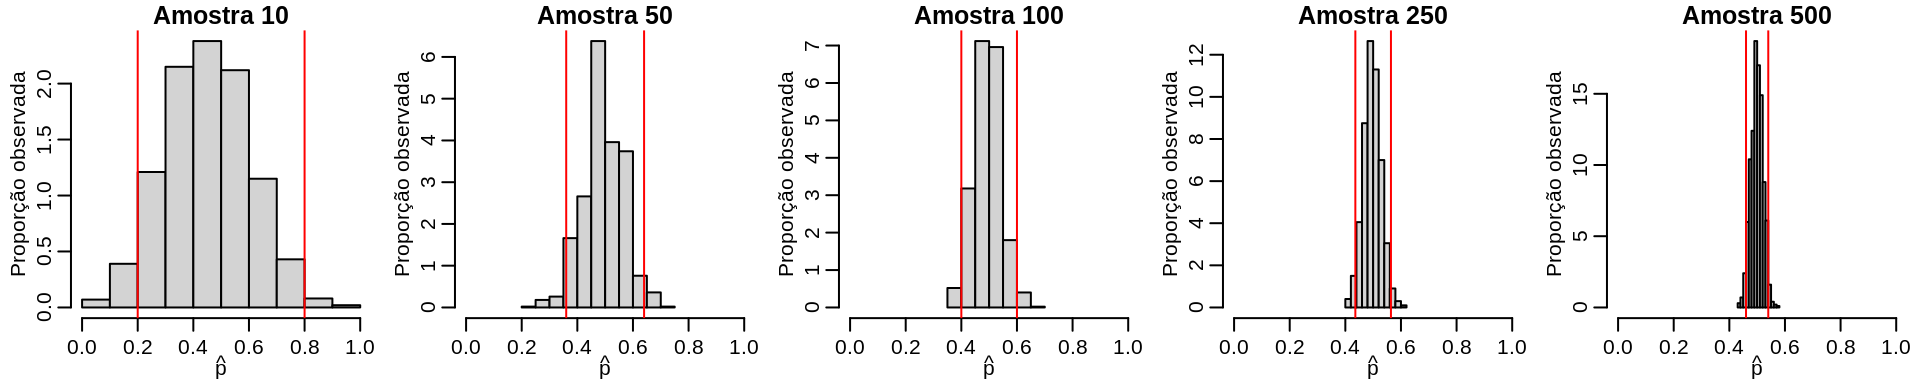
\includegraphics[width=0.99\linewidth]{figures/unnamed-chunk-389-1} \end{center}

Novamente em termos práticos não temos como repetir o experimento um número grande vezes. Assim, recorremos novamente ao Teorema Central do Limite e estabelecemos a região critica de forma aproximada usando a aproximação Gaussiana. No caso Bernoulli, este procedimento resulta na seguinte estatística de teste

\begin{itemize}
\tightlist
\item
  Estatística do teste caso Bernoulli
\end{itemize}

\[
Z = \frac{\hat{p} - p_0}{\sqrt{\frac{p_0(1-p_0)}{n}}} \sim N(0,1).
\]

O procedimento aqui descrito em linhas gerais é bastante genérico e perfaz toda a estatística. No entanto está fora do escopo deste material discutir tais procedimentos em detalhes. Na sequência apresentamos o resumo de alguns casos notáveis de testes de hipóteses que aparecem com frequência em cursos de estatística básica.

\textbf{Exemplo 1} Considere que seja de interesse verificar se existe evidências que o candidato \(X\) vai ganhar as eleições. Em termos estatístico isso significa que

\begin{itemize}
\tightlist
\item
  \(H_0: p = 0.5\) contra \(H_1:p > 0.5.\)
\end{itemize}

Suponha que adotamos \(5\%\) de significância.
Neste caso a região crítica é unilateral, e tem a seguinte forma
\[p_c = 0.5 + 1.64\sqrt{0.25/10} = 0.76.\]
Vamos fazer um gráfico da região de aceitação e rejeição e verificar onde a proporção amostral está localizada para concluir o teste.

\begin{Shaded}
\begin{Highlighting}[]
\FunctionTok{curve}\NormalTok{(}\FunctionTok{dnorm}\NormalTok{(x, }\AttributeTok{mean =} \FloatTok{0.5}\NormalTok{, }\AttributeTok{sd =} \FunctionTok{sqrt}\NormalTok{(}\FloatTok{0.25}\SpecialCharTok{/}\DecValTok{10}\NormalTok{)), }\FloatTok{0.1}\NormalTok{, }\FloatTok{0.9}\NormalTok{, }
      \AttributeTok{ylab =} \StringTok{"Densidade"}\NormalTok{, }\AttributeTok{xlab =} \FunctionTok{expression}\NormalTok{(}\FunctionTok{hat}\NormalTok{(p)))}
\FunctionTok{abline}\NormalTok{(}\AttributeTok{v =} \FloatTok{0.5}\SpecialCharTok{+}\FunctionTok{qnorm}\NormalTok{(}\FloatTok{0.95}\NormalTok{)}\SpecialCharTok{*}\FunctionTok{sqrt}\NormalTok{(}\FloatTok{0.25}\SpecialCharTok{/}\DecValTok{10}\NormalTok{))}
\FunctionTok{abline}\NormalTok{(}\AttributeTok{v =} \DecValTok{6}\SpecialCharTok{/}\DecValTok{10}\NormalTok{, }\AttributeTok{col =} \StringTok{"red"}\NormalTok{, }\AttributeTok{lty =} \DecValTok{2}\NormalTok{, }\AttributeTok{lwd =} \DecValTok{2}\NormalTok{)}
\end{Highlighting}
\end{Shaded}

\begin{center}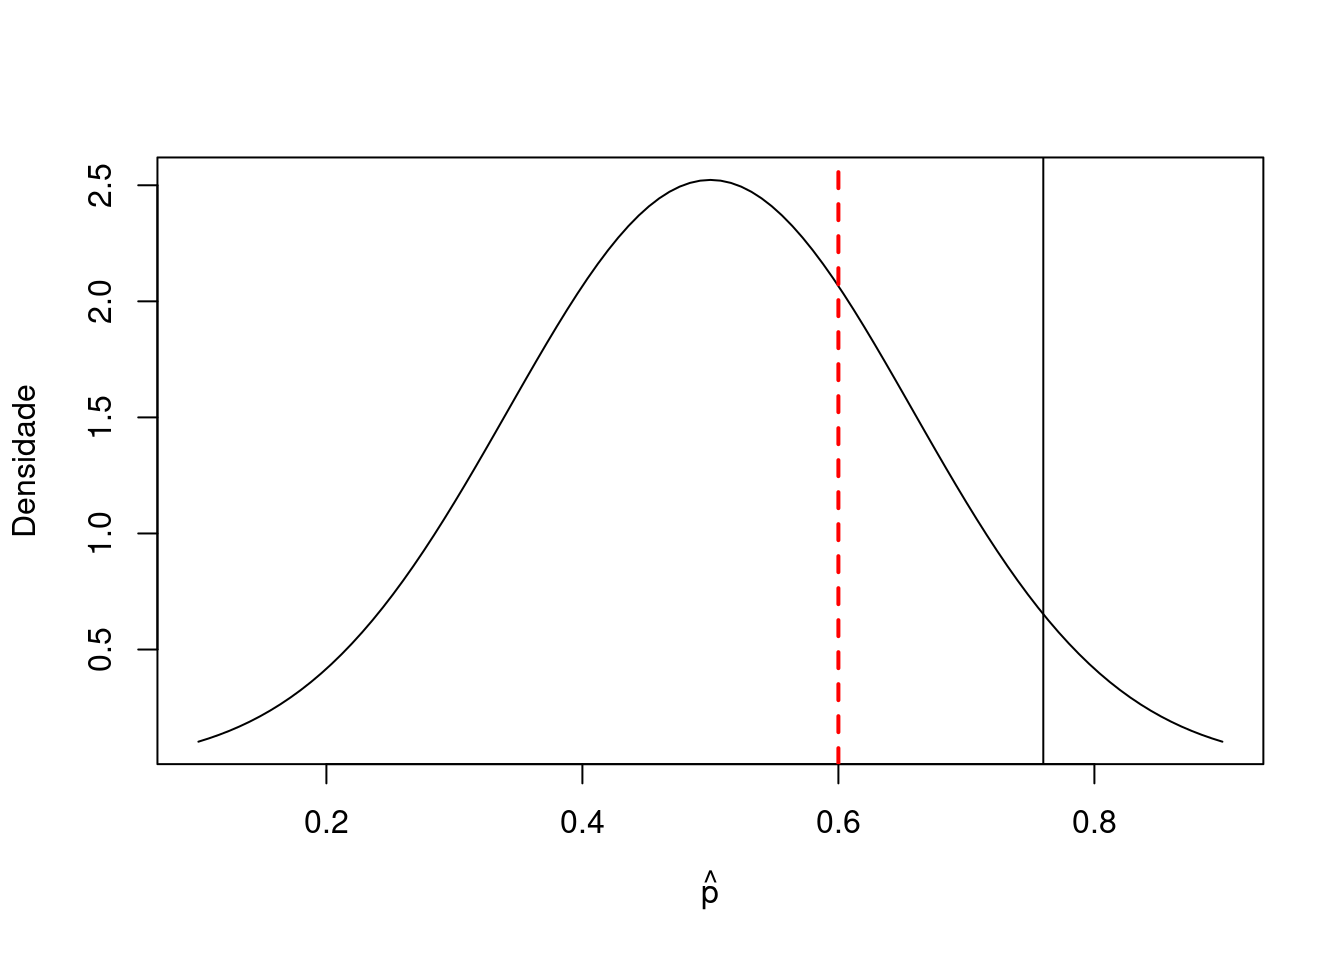
\includegraphics{figures/unnamed-chunk-390-1} \end{center}

Lembre-se que a proporção amostral foi de \(0.6\) em \(10\) entrevistas.
Assim, vemos claramente que não temos evidências para rejeitar \(H_0\).
Neste caso não temos evidências para dizer que o candidato X irá ganhar a eleição.

\begin{itemize}
\tightlist
\item
  Estatística do teste caso Normal
\end{itemize}

No caso de população Normal, a estatística de teste para testar \(H_0:\mu = \mu_0\) contra \(H_1: \mu \neq \mu_0\) com variância conhecida \(\sigma^2\) é dada por

\[
\frac{\hat{y} -  \mu_0}{\sigma/\sqrt{n}} \sim N(0,1)
\]
onde \(\mu_0\) é o valor especificado sob a hipótese nula. Neste caso a região crítica para testes bilaterais toma a seguinte forma:

\[
y_I = \mu_0 - Z_{\alpha/2} \sqrt{\sigma^2 / n}\quad \text{e} \quad y_S = \mu_0 + Z_{\alpha/2} \sqrt{\sigma^2 / n}.
\]

\textbf{Exemplo 2} (Magalhães e Lima, pg. 252). Um pesquisador deseja estudar o efeito de certa substância no tempo de reação de seres vivos a um certo tipo de estímulo. Um experimento é desenvolvido com cobaias que são inoculadas com a substância e submetidas a um estimulo elétrico, com seus tempos de reação (em segundos) anotados. Os seguintes valores foram obtidos: \(9,1;\quad 9,3;\quad 7,2;\quad 7,5;\quad 13,3;\quad 10,9;\quad 7,2;\quad 9,9;\quad 8,0;\quad 8,6\). Admite-se que o tempo de reação segue, em geral o modelo Normal com média 8 e desvio padrão \(\sigma = 2\) segundos. O pesquisador desconfia, entretanto, que o tempo médio sofre alteração por influência da substância. Neste caso as hipóteses de interesse são:

\begin{itemize}
\tightlist
\item
  \(H_0:\) as cobais apresentam tempo de reação padrão;
\item
  \(H_1:\) as cobais tem o tempo de reação alterado.
\end{itemize}

Em termos de modelo estatístico, tais hipóteses são traduzidas para afirmações acerca do parâmetro \(\mu\).

\begin{itemize}
\tightlist
\item
  \(H_0: \mu = 8\) contra \(H_1: \mu \neq 8\).
\end{itemize}

Neste caso a região crítica para \(\alpha = 0,05\) fica dada por
\[y_I = 8 - 1,96\sqrt{4/10} = 6,76 \quad \text{e} \quad y_S = 8 + 1,96 \sqrt{4/10} = 9,24.\]
Vamos agora obter a média amostral e concluir o teste.

\begin{Shaded}
\begin{Highlighting}[]
\NormalTok{x }\OtherTok{\textless{}{-}} \FunctionTok{c}\NormalTok{(}\FloatTok{9.1}\NormalTok{,}\FloatTok{9.3}\NormalTok{,}\FloatTok{7.2}\NormalTok{,}\FloatTok{7.5}\NormalTok{,}\FloatTok{13.3}\NormalTok{,}\FloatTok{10.9}\NormalTok{,}\FloatTok{7.2}\NormalTok{,}\FloatTok{9.9}\NormalTok{,}\FloatTok{8.0}\NormalTok{,}\FloatTok{8.6}\NormalTok{)}
\FunctionTok{mean}\NormalTok{(x)}
\NormalTok{[}\DecValTok{1}\NormalTok{] }\FloatTok{9.1}
\end{Highlighting}
\end{Shaded}

Ilustrando a região crítica

\begin{Shaded}
\begin{Highlighting}[]
\FunctionTok{curve}\NormalTok{(}\FunctionTok{dnorm}\NormalTok{(x, }\AttributeTok{mean =} \DecValTok{8}\NormalTok{, }\AttributeTok{sd =} \FunctionTok{sqrt}\NormalTok{(}\DecValTok{4}\SpecialCharTok{/}\DecValTok{10}\NormalTok{)), }\DecValTok{6}\NormalTok{, }\DecValTok{10}\NormalTok{, }
      \AttributeTok{ylab =} \StringTok{"Densidade"}\NormalTok{, }\AttributeTok{xlab =} \FunctionTok{expression}\NormalTok{(}\FunctionTok{hat}\NormalTok{(y)))}
\FunctionTok{abline}\NormalTok{(}\AttributeTok{v =} \FunctionTok{c}\NormalTok{(}\DecValTok{8}\SpecialCharTok{{-}}\FunctionTok{qnorm}\NormalTok{(}\FloatTok{0.975}\NormalTok{)}\SpecialCharTok{*}\FunctionTok{sqrt}\NormalTok{(}\DecValTok{4}\SpecialCharTok{/}\DecValTok{10}\NormalTok{), }\DecValTok{8}\SpecialCharTok{+}\FunctionTok{qnorm}\NormalTok{(}\FloatTok{0.975}\NormalTok{)}\SpecialCharTok{*}\FunctionTok{sqrt}\NormalTok{(}\DecValTok{4}\SpecialCharTok{/}\DecValTok{10}\NormalTok{) ))}
\FunctionTok{abline}\NormalTok{(}\AttributeTok{v =} \FunctionTok{mean}\NormalTok{(x), }\AttributeTok{col =} \StringTok{"red"}\NormalTok{, }\AttributeTok{lwd =} \DecValTok{2}\NormalTok{, }\AttributeTok{lty =} \DecValTok{2}\NormalTok{)}
\end{Highlighting}
\end{Shaded}

\begin{center}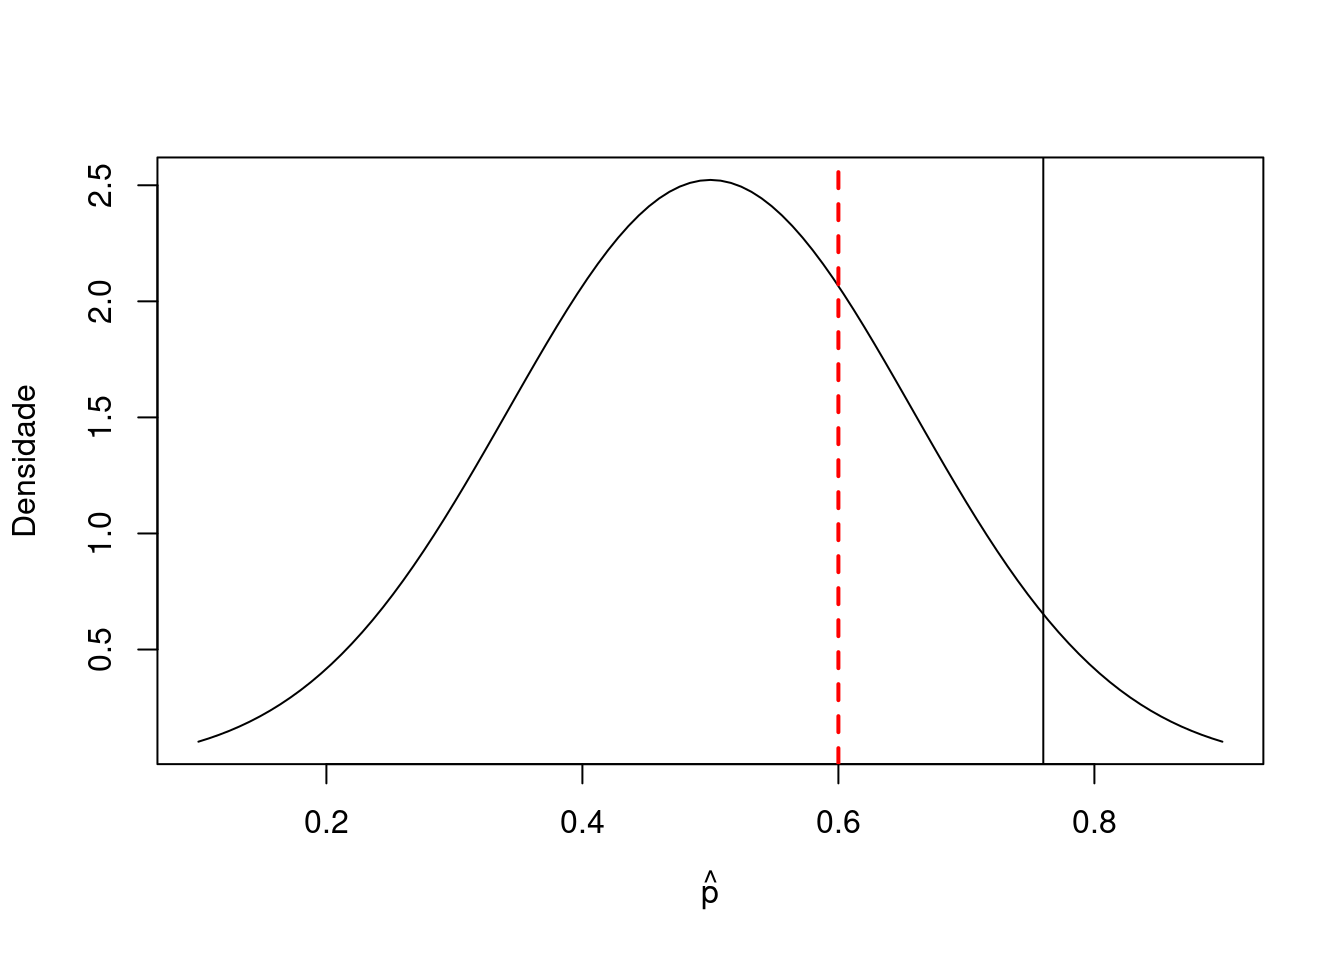
\includegraphics{figures/unnamed-chunk-392-1} \end{center}

Como o valor observado da média amostral pertence a região de aceitação de \(H_0\), aceitamos a hipóteses \(H_0\) ao nível de significância de \(5\%\). Em outras palavras, concluímos que o tempo de reação das cobais submetidas à substância não é alterado.

\hypertarget{teste-t-one-sample-t-test}{%
\subsection{Teste t (one sample t-test)}\label{teste-t-one-sample-t-test}}

\begin{itemize}
\tightlist
\item
  Teste t (one sample t-test)

  \begin{itemize}
  \tightlist
  \item
    Hipóteses: \(H_0: \mu = \mu_0 \quad \times \quad H_1: \mu \neq \mu_0.\)
  \item
    Estatística de teste: \(\frac{\bar{y} - \mu_0}{\hat{\sigma}/\sqrt{n}} \sim t_{n-1}.\)
  \end{itemize}
\item
  Suposições: Para o teste ser exato, precisamos

  \begin{itemize}
  \tightlist
  \item
    \(Y \sim N(\mu, \sigma^2)\) iid.
  \item
    \(\hat{\sigma}^2 = \sum_{i=1}^n (y_i - \bar{y})^2/n-1\).
  \end{itemize}
\item
  Podem ser razoavelmente relaxadas para grandes amostras.
\item
  Neste caso a distribuição t não é mais necessária.
\item
  Assintóticamente a estatística tem distribuição Normal padrão.
\end{itemize}

\textbf{Exemplo 3}: (Magalhães e Lima, pg. 259). Deseja-se investigar se uma certa moléstia que ataca o rim altera o consumo de oxigênio desse orgão. Para indivíduos sadios, admite-se que esse consumo tem distribuição Normal com média 12 \(cm^3/min\). Os valores medidos em cinco pacientes com a moléstia foram: \(14,4;12,9;15,0;13,7;\) e \(13,5\). Qual seria a conclusão, ao nível de 1\(\%\) de significância?

O teste de interesse é

\begin{itemize}
\tightlist
\item
  \(H_0:\) A moléstia não altera a média de consumo renal de oxigênio;
\item
  \(H_1:\) Indivíduos portadores da moléstia têm média alterada.
\end{itemize}

Passando as hipóteses em termos do nosso modelo

\begin{itemize}
\tightlist
\item
  \(H_0: \mu = 12\) contra \(H_1: \mu \neq 12\).
\end{itemize}

O R conta com uma função especifica para este teste, conforme mostra o código abaixo.

\begin{Shaded}
\begin{Highlighting}[]
\NormalTok{y }\OtherTok{\textless{}{-}} \FunctionTok{c}\NormalTok{(}\FloatTok{14.4}\NormalTok{,}\FloatTok{12.9}\NormalTok{,}\DecValTok{15}\NormalTok{,}\FloatTok{13.7}\NormalTok{,}\FloatTok{13.5}\NormalTok{)}
\FunctionTok{t.test}\NormalTok{(}\AttributeTok{x =}\NormalTok{ y, }\AttributeTok{mu =} \DecValTok{12}\NormalTok{)}

\NormalTok{    One Sample t}\SpecialCharTok{{-}}\NormalTok{test}

\NormalTok{data}\SpecialCharTok{:}\NormalTok{  y}
\NormalTok{t }\OtherTok{=} \FloatTok{5.2099}\NormalTok{, df }\OtherTok{=} \DecValTok{4}\NormalTok{, p}\SpecialCharTok{{-}}\NormalTok{value }\OtherTok{=} \FloatTok{0.006472}
\NormalTok{alternative hypothesis}\SpecialCharTok{:}\NormalTok{ true mean is not equal to }\DecValTok{12}
\DecValTok{95}\NormalTok{ percent confidence interval}\SpecialCharTok{:}
 \FloatTok{12.88745} \FloatTok{14.91255}
\NormalTok{sample estimates}\SpecialCharTok{:}
\NormalTok{mean of x }
     \FloatTok{13.9} 
\end{Highlighting}
\end{Shaded}

Neste caso rejeitamos \(H_0\) em favor de \(H_1\). Note que a função retorna uma série de informações úteis. Temos o tipo de teste realizado, o valor da estatística \(t\) e os graus de liberdade do teste ao lado do \(p-valor\). A função já apresenta a conclusão do teste e por reporta o intervalo de confiança para a média amostral e a média amostral.

\hypertarget{teste-t-independent-two-sample-t-test}{%
\subsection{Teste t (independent two sample t-test)}\label{teste-t-independent-two-sample-t-test}}

\begin{itemize}
\tightlist
\item
  Teste t duas populações independentes variâncias iguais (independent two sample t-test)

  \begin{itemize}
  \tightlist
  \item
    Hipóteses: \(H_0: \mu_1 = \mu_2 \quad \times \quad H_1: \mu_1 \neq \mu_2.\)
  \item
    Estatística de teste: \(\frac{\bar{y}_1 - \bar{y}_2}{s_p \sqrt{\frac{1}{n_1} + \frac{1}{n_2}}} \sim t_{n_1 + n_2-2}.\)
  \item
    \(s_p = \sqrt{\frac{(n_1 - 1)s^2_1 + (n_2 - 1)s^2_2}{n_1 + n_2 -2}}\) se variâncias assumidas iguais e tamanhos de amostras diferentes.
  \end{itemize}
\end{itemize}

\textbf{Exemplo 4} Digitadores são treinados em uma empresa em duas turmas distintas. Na primeira, denominada Turma J, utiliza-se um métodos japonês de ensino, ao passo que na segunda turma, denominada Turma A, utiliza-se um método alemão. Deseja-se comparar os dois métodos e para tanto, 16 alunos de cada turma foram escolhidos aleatoriamente e uma mesma tarefa foi atribuída a cada um. Ao final do experimento, o tempo gasto na realização da tarefa, para cada aluno, foi anotado. No processo, dois computadores utilizados pelos alunos selecionados da turma J e três da turma A apresentaram problemas que impediram a realização da tarefa; o tamanho da amostra foi assim reduzido para 14 e 13 respectivamente, para as turmas J e A. Os dados são os seguintes:

\begin{Shaded}
\begin{Highlighting}[]
\NormalTok{J }\OtherTok{\textless{}{-}} \FunctionTok{c}\NormalTok{(}\DecValTok{10}\NormalTok{,}\DecValTok{13}\NormalTok{,}\DecValTok{9}\NormalTok{,}\DecValTok{10}\NormalTok{,}\DecValTok{14}\NormalTok{,}\DecValTok{13}\NormalTok{,}\DecValTok{10}\NormalTok{,}\DecValTok{15}\NormalTok{,}\DecValTok{12}\NormalTok{,}\DecValTok{10}\NormalTok{,}\DecValTok{9}\NormalTok{,}\DecValTok{10}\NormalTok{,}\DecValTok{13}\NormalTok{,}\DecValTok{14}\NormalTok{)}
\NormalTok{A }\OtherTok{\textless{}{-}} \FunctionTok{c}\NormalTok{(}\DecValTok{15}\NormalTok{,}\DecValTok{12}\NormalTok{,}\DecValTok{18}\NormalTok{,}\DecValTok{16}\NormalTok{,}\DecValTok{15}\NormalTok{,}\DecValTok{17}\NormalTok{,}\DecValTok{17}\NormalTok{,}\DecValTok{15}\NormalTok{,}\DecValTok{16}\NormalTok{,}\DecValTok{17}\NormalTok{,}\DecValTok{11}\NormalTok{,}\DecValTok{17}\NormalTok{,}\DecValTok{14}\NormalTok{,}\ConstantTok{NA}\NormalTok{)}
\NormalTok{dplyr}\SpecialCharTok{::}\FunctionTok{tibble}\NormalTok{(J,A)}
\CommentTok{\# A tibble: 14 x 2}
\NormalTok{       J     A}
   \SpecialCharTok{\textless{}}\NormalTok{dbl}\SpecialCharTok{\textgreater{}} \ErrorTok{\textless{}}\NormalTok{dbl}\SpecialCharTok{\textgreater{}}
 \DecValTok{1}    \DecValTok{10}    \DecValTok{15}
 \DecValTok{2}    \DecValTok{13}    \DecValTok{12}
 \DecValTok{3}     \DecValTok{9}    \DecValTok{18}
 \DecValTok{4}    \DecValTok{10}    \DecValTok{16}
 \DecValTok{5}    \DecValTok{14}    \DecValTok{15}
 \DecValTok{6}    \DecValTok{13}    \DecValTok{17}
 \DecValTok{7}    \DecValTok{10}    \DecValTok{17}
 \DecValTok{8}    \DecValTok{15}    \DecValTok{15}
 \DecValTok{9}    \DecValTok{12}    \DecValTok{16}
\DecValTok{10}    \DecValTok{10}    \DecValTok{17}
\DecValTok{11}     \DecValTok{9}    \DecValTok{11}
\DecValTok{12}    \DecValTok{10}    \DecValTok{17}
\DecValTok{13}    \DecValTok{13}    \DecValTok{14}
\DecValTok{14}    \DecValTok{14}    \ConstantTok{NA}
\end{Highlighting}
\end{Shaded}

Apesar de não conhecidas, as variâncias populacionais são assumidas iguais com base em estudos anteriores. Suponha que o interesse é testar

\begin{itemize}
\tightlist
\item
  \(H_0: \mu_J = \mu_A\) contra \(H_1: \mu_J \neq \mu_A\).
\end{itemize}

\begin{Shaded}
\begin{Highlighting}[]
\FunctionTok{t.test}\NormalTok{(}\AttributeTok{x =}\NormalTok{ J, }\AttributeTok{y =}\NormalTok{ A, }\AttributeTok{paired =} \ConstantTok{FALSE}\NormalTok{, }\AttributeTok{var.equal =} \ConstantTok{TRUE}\NormalTok{)}

\NormalTok{    Two Sample t}\SpecialCharTok{{-}}\NormalTok{test}

\NormalTok{data}\SpecialCharTok{:}\NormalTok{  J and A}
\NormalTok{t }\OtherTok{=} \SpecialCharTok{{-}}\FloatTok{4.7965}\NormalTok{, df }\OtherTok{=} \DecValTok{25}\NormalTok{, p}\SpecialCharTok{{-}}\NormalTok{value }\OtherTok{=} \FloatTok{6.313e{-}05}
\NormalTok{alternative hypothesis}\SpecialCharTok{:}\NormalTok{ true difference }\ControlFlowTok{in}\NormalTok{ means is not equal to }\DecValTok{0}
\DecValTok{95}\NormalTok{ percent confidence interval}\SpecialCharTok{:}
 \SpecialCharTok{{-}}\FloatTok{5.450501} \SpecialCharTok{{-}}\FloatTok{2.175872}
\NormalTok{sample estimates}\SpecialCharTok{:}
\NormalTok{mean of x mean of y }
 \FloatTok{11.57143}  \FloatTok{15.38462} 
\end{Highlighting}
\end{Shaded}

\hypertarget{teste-t-variuxe2ncia-diferentes}{%
\subsection{Teste t variância diferentes}\label{teste-t-variuxe2ncia-diferentes}}

\begin{itemize}
\tightlist
\item
  Teste t duas populações independentes variâncias diferentes (independent two sample t-test)

  \begin{itemize}
  \tightlist
  \item
    Hipóteses: \(H_0: \mu_1 = \mu_2 \quad \times \quad H_1: \mu_1 \neq \mu_2.\)
  \item
    Estatística de teste: \(\frac{\bar{y}_1 - \bar{y}_2}{s_{\delta}} \sim t_{df}.\)
  \item
    \(s_{\delta} = \sqrt{\frac{s^1}{n_1} + \frac{s^2}{n_2}}\) se variâncias diferentes e tamanhos de amostras diferentes.
  \item
    Graus de liberdade \(df = \frac{\left ( \frac{s^2_1}{n_1} + \frac{s^2_2}{n_2} \right )}{\frac{(s^2_1/n_1)^2}{n_1 - 1} + \frac{(s^2_2/n_2)^2}{n_2 - 1}}.\)
  \end{itemize}
\end{itemize}

\textbf{Exemplo 5} Considere o exemplo dos digitadores, porém agora sem assumir que as variâncias populacionais são iguais. O teste t neste caso pode ser realizado da seguinte forma:

\begin{Shaded}
\begin{Highlighting}[]
\FunctionTok{t.test}\NormalTok{(}\AttributeTok{x =}\NormalTok{ J, }\AttributeTok{y =}\NormalTok{ A, }\AttributeTok{paired =} \ConstantTok{FALSE}\NormalTok{, }\AttributeTok{var.equal =} \ConstantTok{FALSE}\NormalTok{)}

\NormalTok{    Welch Two Sample t}\SpecialCharTok{{-}}\NormalTok{test}

\NormalTok{data}\SpecialCharTok{:}\NormalTok{  J and A}
\NormalTok{t }\OtherTok{=} \SpecialCharTok{{-}}\FloatTok{4.7967}\NormalTok{, df }\OtherTok{=} \FloatTok{24.856}\NormalTok{, p}\SpecialCharTok{{-}}\NormalTok{value }\OtherTok{=} \FloatTok{6.399e{-}05}
\NormalTok{alternative hypothesis}\SpecialCharTok{:}\NormalTok{ true difference }\ControlFlowTok{in}\NormalTok{ means is not equal to }\DecValTok{0}
\DecValTok{95}\NormalTok{ percent confidence interval}\SpecialCharTok{:}
 \SpecialCharTok{{-}}\FloatTok{5.450930} \SpecialCharTok{{-}}\FloatTok{2.175444}
\NormalTok{sample estimates}\SpecialCharTok{:}
\NormalTok{mean of x mean of y }
 \FloatTok{11.57143}  \FloatTok{15.38462} 
\end{Highlighting}
\end{Shaded}

\hypertarget{teste-t-pareado}{%
\subsection{Teste t pareado}\label{teste-t-pareado}}

\begin{itemize}
\tightlist
\item
  Teste t duas populações dependentes (paired two sample t-test)

  \begin{itemize}
  \tightlist
  \item
    Hipóteses: \(H_0: \mu_D = 0 \quad \times \quad H_1: \mu_D \neq 0.\)
  \item
    Estatística de teste: \(\frac{\bar{y}_D - 0}{\hat{\sigma}_D/\sqrt{n}} \sim t_{n-1}.\)
  \item
    Neste caso, \(\mu_D\) e \(\hat{\sigma}_D\) são a média e o desvio-padrão da diferença entre \(y_1\) e \(y_2\).
  \end{itemize}
\end{itemize}

\textbf{Exemplo 6} Uma distribuidora de combustíveis deseja verificar se um novo tipo de gasolina é eficaz na revitalização de moteores velhos. Com esse objetivo, seleciona 12 automóveis de um mesmo modelo com mais de 8 anos de uso e, após regulagem de seus motores, verifica o consumo de combustível. Em seguida, o carro é abastecido com o novo tipo de combustível durante 15 semanas, e uma nova aferição do consumo é feita. Defina as variáveis aleatórias \(X_i\) e \(Y_i\) como o rendimento do automóvel \(i\) respectivamente antes e após as 15 semanas. Vemos que \(X_i\) e \(Y_i\) foram medidas em uma mesma unidade amostral e, assim, é razoável assumir que exista alguma dependência entre elas. Os valores observados, em \(km/l\), junto com as diferenças \(D_i = Y_i - X_i\), para os 12 automóveis são apresentados na tabela a seguir.

\begin{Shaded}
\begin{Highlighting}[]
\NormalTok{Apos }\OtherTok{\textless{}{-}} \FunctionTok{c}\NormalTok{(}\FloatTok{11.6}\NormalTok{,}\FloatTok{8.8}\NormalTok{,}\FloatTok{9.9}\NormalTok{,}\FloatTok{9.5}\NormalTok{,}\FloatTok{11.6}\NormalTok{,}\FloatTok{9.1}\NormalTok{,}\FloatTok{10.6}\NormalTok{,}\FloatTok{10.8}\NormalTok{,}\FloatTok{13.4}\NormalTok{,}\FloatTok{10.6}\NormalTok{,}\FloatTok{10.5}\NormalTok{,}\FloatTok{11.4}\NormalTok{)}
\NormalTok{Antes }\OtherTok{\textless{}{-}} \FunctionTok{c}\NormalTok{(}\FloatTok{8.1}\NormalTok{,}\FloatTok{7.9}\NormalTok{,}\FloatTok{6.8}\NormalTok{,}\FloatTok{7.8}\NormalTok{,}\FloatTok{7.6}\NormalTok{,}\FloatTok{7.9}\NormalTok{,}\FloatTok{5.7}\NormalTok{,}\FloatTok{8.4}\NormalTok{,}\DecValTok{8}\NormalTok{,}\FloatTok{9.5}\NormalTok{,}\DecValTok{8}\NormalTok{,}\FloatTok{6.8}\NormalTok{)}
\NormalTok{D }\OtherTok{\textless{}{-}}\NormalTok{ Apos }\SpecialCharTok{{-}}\NormalTok{ Antes}
\NormalTok{dplyr}\SpecialCharTok{::}\FunctionTok{tibble}\NormalTok{(Apos, Antes, D)}
\CommentTok{\# A tibble: 12 x 3}
\NormalTok{    Apos Antes     D}
   \SpecialCharTok{\textless{}}\NormalTok{dbl}\SpecialCharTok{\textgreater{}} \ErrorTok{\textless{}}\NormalTok{dbl}\SpecialCharTok{\textgreater{}} \ErrorTok{\textless{}}\NormalTok{dbl}\SpecialCharTok{\textgreater{}}
 \DecValTok{1}  \FloatTok{11.6}   \FloatTok{8.1}   \FloatTok{3.5}
 \DecValTok{2}   \FloatTok{8.8}   \FloatTok{7.9}   \FloatTok{0.9}
 \DecValTok{3}   \FloatTok{9.9}   \FloatTok{6.8}   \FloatTok{3.1}
 \DecValTok{4}   \FloatTok{9.5}   \FloatTok{7.8}   \FloatTok{1.7}
 \DecValTok{5}  \FloatTok{11.6}   \FloatTok{7.6}   \DecValTok{4}  
 \DecValTok{6}   \FloatTok{9.1}   \FloatTok{7.9}   \FloatTok{1.2}
 \DecValTok{7}  \FloatTok{10.6}   \FloatTok{5.7}   \FloatTok{4.9}
 \DecValTok{8}  \FloatTok{10.8}   \FloatTok{8.4}   \FloatTok{2.4}
 \DecValTok{9}  \FloatTok{13.4}   \DecValTok{8}     \FloatTok{5.4}
\DecValTok{10}  \FloatTok{10.6}   \FloatTok{9.5}   \FloatTok{1.1}
\DecValTok{11}  \FloatTok{10.5}   \DecValTok{8}     \FloatTok{2.5}
\DecValTok{12}  \FloatTok{11.4}   \FloatTok{6.8}   \FloatTok{4.6}
\end{Highlighting}
\end{Shaded}

Queremos testar as hipóteses
- \(H_0:\) \(\mu_D = 0\) (a intervenção não produz efeito)
- \(H_1:\) \(\mu_D \neq 0\) (a intervenção produz algum efeito)

\begin{Shaded}
\begin{Highlighting}[]
\FunctionTok{t.test}\NormalTok{(}\AttributeTok{x =}\NormalTok{ Apos, }\AttributeTok{y =}\NormalTok{ Antes, }\AttributeTok{paired =} \ConstantTok{TRUE}\NormalTok{)}

\NormalTok{    Paired t}\SpecialCharTok{{-}}\NormalTok{test}

\NormalTok{data}\SpecialCharTok{:}\NormalTok{  Apos and Antes}
\NormalTok{t }\OtherTok{=} \FloatTok{6.5396}\NormalTok{, df }\OtherTok{=} \DecValTok{11}\NormalTok{, p}\SpecialCharTok{{-}}\NormalTok{value }\OtherTok{=} \FloatTok{4.195e{-}05}
\NormalTok{alternative hypothesis}\SpecialCharTok{:}\NormalTok{ true mean difference is not equal to }\DecValTok{0}
\DecValTok{95}\NormalTok{ percent confidence interval}\SpecialCharTok{:}
 \FloatTok{1.951609} \FloatTok{3.931724}
\NormalTok{sample estimates}\SpecialCharTok{:}
\NormalTok{mean difference }
       \FloatTok{2.941667} 
\end{Highlighting}
\end{Shaded}

\hypertarget{teste-f}{%
\subsection{Teste F}\label{teste-f}}

\begin{itemize}
\tightlist
\item
  Teste F para igualdade de variâncias.

  \begin{itemize}
  \tightlist
  \item
    Hipóteses: \(H_0: \sigma^2_1 = \sigma^2_2 \quad \times H_1: \sigma^2_1 \neq \sigma^2_2\).
  \item
    Estatística de teste: \(F = \frac{s^2_1}{s^2_2} \sim F_{(n_1-1)(n_2-1)}\).
  \item
    Suposições \(Y_1 \sim N(\mu_1, \sigma^2_1)\) e \(Y_2 \sim N(\mu_2, \sigma^2_2)\).
  \item
    Em geral, este teste é conhecido por ser sensível a suposição de normalidade.
  \end{itemize}
\item
  Se normalidade é duvidosa, use o teste para variâncias diferentes.
\item
  Poder e tamanho do teste podem ser altamente sensíveis a suposições.
\item
  Para grandes amostras o TCL fornece uma opção robusta a não-normalidade.
\item
  \textbf{Regra do dedão} Amostra maior que \(30\) TCL funciona bem!
\item
  Mas cuidado!! depende da situação!!
\end{itemize}

\textbf{Exemplo 7} Sabe-se que em uma região do país a altura média é de \(1,68\)m, com variância de \(0,30m^2\). Um pesquisador acredita que a alimentação rotineira em uma cidade litorânea, sendo diferente da região como um todo, contribui para que as pessoas apresentem alturas mais homogêneas, apesar de não alterar a altura média da população da cidade. Para verificar sua suspeita, ele coletou um amostra de 31 pessoas e obteve
a seguinte amostra:

\begin{Shaded}
\begin{Highlighting}[]
\NormalTok{y }\OtherTok{\textless{}{-}} \FunctionTok{c}\NormalTok{(}\FloatTok{1.77}\NormalTok{, }\FloatTok{1.72}\NormalTok{, }\FloatTok{2.39}\NormalTok{, }\FloatTok{1.95}\NormalTok{, }\FloatTok{1.69}\NormalTok{, }\FloatTok{1.84}\NormalTok{, }\FloatTok{1.86}\NormalTok{, }\FloatTok{1.57}\NormalTok{, }\FloatTok{1.38}\NormalTok{, }\FloatTok{1.47}\NormalTok{, }\FloatTok{1.94}\NormalTok{, }
       \FloatTok{1.15}\NormalTok{, }\FloatTok{1.93}\NormalTok{, }\FloatTok{2.18}\NormalTok{, }\FloatTok{1.37}\NormalTok{, }\FloatTok{1.56}\NormalTok{, }\FloatTok{1.28}\NormalTok{, }\FloatTok{1.81}\NormalTok{, }\FloatTok{1.66}\NormalTok{, }\FloatTok{1.99}\NormalTok{, }\FloatTok{2.07}\NormalTok{, }\FloatTok{1.67}\NormalTok{, }
       \FloatTok{1.40}\NormalTok{, }\FloatTok{1.03}\NormalTok{, }\FloatTok{1.58}\NormalTok{, }\FloatTok{1.99}\NormalTok{, }\FloatTok{1.48}\NormalTok{, }\FloatTok{1.73}\NormalTok{, }\FloatTok{1.44}\NormalTok{, }\FloatTok{1.35}\NormalTok{, }\FloatTok{1.54}\NormalTok{)}
\end{Highlighting}
\end{Shaded}

Além disso, coletou um conjunto de 20 observações da população geral.

\begin{Shaded}
\begin{Highlighting}[]
\FunctionTok{set.seed}\NormalTok{(}\DecValTok{123}\NormalTok{)}
\NormalTok{x }\OtherTok{\textless{}{-}} \FunctionTok{rnorm}\NormalTok{(}\DecValTok{20}\NormalTok{, }\AttributeTok{mean =} \FloatTok{1.68}\NormalTok{, }\AttributeTok{sd =} \FloatTok{0.30}\NormalTok{)}
\end{Highlighting}
\end{Shaded}

Realize um teste de hipótese para verificar
- \(H_0: \sigma^2 = 0,30\) contra \(H_1: \sigma^2 < 0,30\).

\begin{Shaded}
\begin{Highlighting}[]
\FunctionTok{var.test}\NormalTok{(y, x, }\AttributeTok{alternative =} \StringTok{"less"}\NormalTok{)}

\NormalTok{    F test to compare two variances}

\NormalTok{data}\SpecialCharTok{:}\NormalTok{  y and x}
\NormalTok{F }\OtherTok{=} \FloatTok{1.1044}\NormalTok{, num df }\OtherTok{=} \DecValTok{30}\NormalTok{, denom df }\OtherTok{=} \DecValTok{19}\NormalTok{, p}\SpecialCharTok{{-}}\NormalTok{value }\OtherTok{=} \FloatTok{0.5811}
\NormalTok{alternative hypothesis}\SpecialCharTok{:}\NormalTok{ true ratio of variances is less than }\DecValTok{1}
\DecValTok{95}\NormalTok{ percent confidence interval}\SpecialCharTok{:}
 \FloatTok{0.000000} \FloatTok{2.148239}
\NormalTok{sample estimates}\SpecialCharTok{:}
\NormalTok{ratio of variances }
           \FloatTok{1.10436} 
\end{Highlighting}
\end{Shaded}

\hypertarget{exercuxedcios-19}{%
\section*{Exercícios}\label{exercuxedcios-19}}


\begin{enumerate}
\def\labelenumi{\arabic{enumi}.}
\tightlist
\item
  Uma empresa de pesquisa de mercado usou uma amostra de indivíduos para avaliar o potencial de compra de determinado produto antes e depois de as pessoas virem um novo comercial de televisão a respeito do produto. As avaliações do potencial de compra basearam-se em uma escala de 0 a 10, e os valores mais altos indicavam maior potencial de compra. A hipótese nula declarava que a avaliação média depois seria igual a avaliação média antes. A rejeição dessa hipótese demonstraria que o comercial melhorou a avaliação do potencial médio de compra. Use \(\alpha = 0,05\) e os dados apresentados abaixo para testar a hipótese e comentar o valor do comercial.
\end{enumerate}

\begin{verbatim}
# A tibble: 8 x 3
    ind Depois Antes
  <int>  <dbl> <dbl>
1     1      6     5
2     2      6     4
3     3      7     7
4     4      4     3
5     5      3     5
6     6      9     8
7     7      7     5
8     8      6     6
\end{verbatim}

\begin{enumerate}
\def\labelenumi{\arabic{enumi}.}
\setcounter{enumi}{1}
\tightlist
\item
  Os preços por galçao (3,78 litros) de gasolina para carros de aluguel foram amostrados em oito grandes aeroportos. Os dados relativos às empresas de carros de aluguel Hertz e National são apresentados a seguir
\end{enumerate}

\begin{verbatim}
# A tibble: 8 x 3
  Aero                     Hertz National
  <chr>                    <dbl>    <dbl>
1 "Boston"                  1.55     1.56
2 "Chicago"                 1.62     1.59
3 " Los Angeles"            1.72     1.78
4 "Miami"                   1.65     1.49
5 "Nova York (JFK)"         1.72     1.51
6 "Nova York (La Guardia)"  1.67     1.5 
7 "Orange County"           1.68     1.77
8 "Washington"              1.52     1.41
\end{verbatim}

Use \(\alpha = 0,05\) para testar a hipótese de que não há diferença entre os preços médios populacionais por galão em relação às duas empresas.

\begin{enumerate}
\def\labelenumi{\arabic{enumi}.}
\setcounter{enumi}{2}
\tightlist
\item
  Na Western University, a média histórica das pontuações nos exames para obtenção de bolsas de estudo correspondente às inscrições feitas por calouros é 900. Presume-se que o desvio padrão histórico da população é \(\sigma = 180\) seja conhecido. Anualmente, o vice-reitor usa uma amostra das inscrições para determinar se a média da pontuação nos exames dos calouros se modificou.

  \begin{itemize}
  \tightlist
  \item
    Estabeleça as hipóteses.
  \item
    Qual é a estimação pontual e o intervalo de confiança de \(95\%\) da média populacional nos exames se a seguinte amostra de tamanho 50 for observada.
  \end{itemize}
\end{enumerate}

\begin{verbatim}
# A tibble: 10 x 1
   `matrix(x, 10, 5)`[,1]  [,2]  [,3]  [,4]  [,5]
                    <dbl> <dbl> <dbl> <dbl> <dbl>
 1                   799. 1120.  708.  977.  775.
 2                   859.  965.  861.  847.  863.
 3                  1181.  972.  715. 1061.  672.
 4                   913.  920.  769. 1058. 1290.
 5                   923.  800.  787. 1048. 1117.
 6                  1209. 1222.  596. 1024.  698.
 7                   983.  990. 1051. 1000.  827.
 8                   672.  546.  928.  889.  816.
 9                   776. 1026.  695.  845. 1040.
10                   820.  815. 1126.  832.  885.
\end{verbatim}

\begin{itemize}
\tightlist
\item
  Realize um teste de hipótese para verificar a suspeita do vice-reitor. Use \(\alpha = 0,05\). Qual é a sua conclusão?
\end{itemize}

\begin{enumerate}
\def\labelenumi{\arabic{enumi}.}
\setcounter{enumi}{3}
\tightlist
\item
  Mensalmente o governo federal publica uma série de estatísticas sobre o número de pessoas que estão desempregadas e a média de tempo em que estão desempregadas. Em relação a novembro de 1998, o governo divulgou que a duração média nacional de desemprego era 14,6 semanas. O prefeito de Curitiba solicitou um estudo sobre a situação de desemprego na cidade. Uma amostra de 50 habitantes desempregados em Curitiba incluiu dados sobre a idade e o número de semanas em que estavam desempregados. O conjunto de dados é apresentado abaixo:
\end{enumerate}

\begin{verbatim}
   Idade.1.10. Semanas.1.10. Idade.11.20. Semanas.11.20. Idade.21.30.
1           36             9           32              7           30
2           34             7           47              8           38
3           34             7           27              8           34
4           43            11           36              9           30
5           33            12           37             12           36
6           43             6           35              9           34
7           25            13           40              7           35
8           28            10           47              8           37
9           36             9           32              4           32
10          37             4           29              6           30
   Semanas.21.30. Idade.31.40. Semanas.31.40. Idade.41.50. Semanas.41.50.
1               7           36             10           32             10
2               6           41              7           44              5
3              11           37             14           33              7
4               5           33             14           28              8
5              10           41             10           45             11
6               8           40              6           35             12
7               9           38              6           41             11
8               5           36              9           31              9
9               9           31              6           34             13
10              6           42              8           30              8
\end{verbatim}

\begin{itemize}
\tightlist
\item
  Use estatísticas descritivas para resumir os dados.
\item
  Desenvolva uma estimação por intervalo de confiança de \(95\%\) da média de idade e semanas desempregadas em Curitiba.
\item
  Realize um teste de hipótese para determinar se a duração média do desemprego em Curitiba é maior que a duração média nacional de 14,6 semanas. Use um nível de confiança de 0,01. Qual a sua conclusão.
\item
  Há uma relação entre a idade do individuo desempregado e o número de semanas de desemprego? Explique.
\end{itemize}

\hypertarget{appendix-apuxeandice}{%
\appendix}


\hypertarget{documentos-dinuxe2micos}{%
\chapter{Documentos dinâmicos}\label{documentos-dinuxe2micos}}

A ideia geral de um documento dinâmico é a de que ele pode ser gerado a
partir de um \textbf{código-fonte}:

\begin{itemize}
\tightlist
\item
  Da mesma forma que um \emph{software} possui seu código-fonte, um documento
  dinâmico é o código-fonte de um relatório.
\item
  É uma combinação de código de computador e as correspondentes
  narrativas descrevendo o resultado que o código está gerando (números,
  tabelas, figuras, \ldots).
\item
  Quando \textbf{compilamos} o documento dinâmico, o código de computador é
  executado, e as saídas são apresentadas. Portanto obtemos um documento
  final que mistura \textbf{código} e \textbf{texto}.
\end{itemize}

Como gerenciamos apenas o código-fonte do documento, ficamos livres de
etapas manuais como ter que refazer um gráfico ou uma tabela após
qualquer alteração na análise.

\hypertarget{literate-programming}{%
\section{Literate Programming}\label{literate-programming}}

\begin{quote}
\emph{Instead of imagining that our main task is to instruct a computer what
to do, let us concentrate rather on explaining to humans what we want
the computer to do.}

\begin{quote}
Donald Knuth
\end{quote}
\end{quote}

O ideia básica por trás de documentos dinâmicos decorre diretamente do
conceito de \emph{literate programming} (``programação letrada''), um paradigma
concebido por \href{https://en.wikipedia.org/wiki/Donald_Knuth}{Donald Knuth} em 1984.

O objetivo da \emph{literate programming} é criar um documento que
``entrelaça'' (mistura) texto e código. O texto é legível para humanos e o
código é legível para máquinas. A análise é descrita em uma série de
texto e blocos de código (\emph{code chunks}). Cada bloco de código irá
executar uma etapa da análise, e estará diretamente associado ao texto
explicativo acima ou abaixo do bloco.

O processo de \emph{literate programming} ocorre em duas vias, chamadas de
\textbf{weaving} e \textbf{tangling}. O importante é que, \textbf{com um único
código-fonte} podemos:

\begin{itemize}
\tightlist
\item
  Produzir documentos para humanos (HTML, PDF, \ldots) \(\Rightarrow\) \emph{weave}
\item
  Produzir ``documentos'' (\emph{scripts}) para máquinas (código) \(\Rightarrow\)
  \emph{tangle}
\end{itemize}

Para podermos usar um sistema como esse, é necessário então uma
linguagem de documentação para humanos (\emph{e.g.} LaTeX ou Markdown), e
uma linguagem de programação que será compilada com o documento (\emph{e.g.}
R ou Python).

Knuth criou inicialmente um sistema chamado \textbf{WEB} para fazer essa
mistura dos seus textos em \(TeX\) com a linguagem Pascal. Atualmente
muitos outros sistemas existem para misturar códigos com texto em várias
linguagens de documentação e de programação.

\hypertarget{literate-programming-no-r}{%
\section{Literate Programming no R}\label{literate-programming-no-r}}

Com a ascensão do R no início dos anos 2000, \href{http://www.statistik.lmu.de/~leisch}{Friedrich Leisch} criou
o \href{https://www.statistik.lmu.de/~leisch/Sweave}{Sweave} em 2002

\begin{itemize}
\tightlist
\item
  S + weave
\item
  Permite ``entrelaçar'' textos do LaTeX com códigos do R
\item
  Ainda é muito utilizado e já é distribuído como uma função do R
  dentro do pacote \texttt{utils}
\end{itemize}

No final de 2011, \href{http://yihui.name/}{Yihui Xie} criou o pacote \href{http://yihui.name/knitr}{knitr} como uma extensão
do Sweave, e com a proposta de ser mais flexível, fácil e \textbf{preparado
para a Web}. Segundo o próprio autor, o knitr é resultado dessa
equação:

\begin{Shaded}
\begin{Highlighting}[]
\NormalTok{knitr }\OtherTok{=}\NormalTok{ Sweave }\SpecialCharTok{+}\NormalTok{ cacheSweave }\SpecialCharTok{+}\NormalTok{ pgfSweave }\SpecialCharTok{+}\NormalTok{ weaver }\SpecialCharTok{+}
\NormalTok{    animation}\SpecialCharTok{::}\NormalTok{saveLatex }\SpecialCharTok{+}\NormalTok{ R2HTML}\SpecialCharTok{::}\NormalTok{RweaveHTML }\SpecialCharTok{+}
\NormalTok{    highlight}\SpecialCharTok{::}\NormalTok{HighlightWeaveLatex }\SpecialCharTok{+} \FloatTok{0.2} \SpecialCharTok{*}\NormalTok{ brew }\SpecialCharTok{+}
    \FloatTok{0.1} \SpecialCharTok{*}\NormalTok{ SweaveListingUtils }\SpecialCharTok{+}\NormalTok{ more}
\end{Highlighting}
\end{Shaded}

Resumidamente, o knitr possui as seguintes vantagens sob o Sweave:

\begin{itemize}
\tightlist
\item
  knit + R
\item
  Uma re-implementação mais moderna do Sweave
\item
  Permite ``entrelaçar'' textos do LaTeX, HTML e \textbf{Markdown} com
  códigos do R
\item
  Também permite misturar texto com códigos de \textbf{outras linguagens}:
  Python, awk, C++, shell.
\item
  Adiciona muitas facilidades como

  \begin{itemize}
  \tightlist
  \item
    Cache
  \item
    Decoração e formatação automática de códigos
  \item
    Geração de gráficos mais direta
  \end{itemize}
\end{itemize}

Podemos fazer uma comparação entre arquivos LaTeX escritos em Sweave
e knitr. Exemplos simples podem ser vistos nos arquivos
\href{exemplos/Exemplo0-Sweave.Rnw}{Exemplo0-Sweave.Rnw} escrito com Sweave e
\href{exemplos/Exemplo0-knitr.Rnw}{Exemplo0-knitr.Rnw} escrito com a sintaxe
do knitr. Para compilar estes documentos, usamos

\begin{Shaded}
\begin{Highlighting}[]
\FunctionTok{Sweave}\NormalTok{(}\StringTok{"Exemplo0{-}Sweave.Rnw"}\NormalTok{)}
\FunctionTok{library}\NormalTok{(knitr)}
\FunctionTok{knit}\NormalTok{(}\StringTok{"Exemplo0{-}knitr.Rnw"}\NormalTok{)}
\end{Highlighting}
\end{Shaded}

Posteriormente, os arquivos \texttt{.tex} gerados podem ser compilados com
qualquer distribuição LaTeX, (\emph{e.g} TeXLive, MikTeX), por exemplo

\begin{Shaded}
\begin{Highlighting}[]
\ExtensionTok{pdflatex}\NormalTok{ Exemplo0{-}Sweave.Rnw}
\ExtensionTok{pdflatex}\NormalTok{ Exemplo0{-}knitr.Rnw}
\end{Highlighting}
\end{Shaded}

Os resultados podem ser vistos nos respectivos arquivos:
\href{exemplos/Exemplo0-Sweave.pdf}{Exemplo0-Sweave.pdf} e
\href{exemplos/Exemplo0-knitr.pdf}{Exemplo0-knitr.pdf}

\hypertarget{markdown}{%
\section{Markdown}\label{markdown}}

Segundo o próprio criador da linguagem:

\begin{quote}
\emph{Markdown is a text-to-HTML conversion tool for web writers. Markdown
allows you to write using an easy-to-read, easy-to-write plain text
format, then convert it to structurally valid XHTML (or HTML).}

\begin{quote}
John Gruber
\end{quote}
\end{quote}

\begin{itemize}
\tightlist
\item
  \href{http://daringfireball.net/projects/markdown}{Markdown} é uma \href{https://pt.wikipedia.org/wiki/Linguagem_de_marcação/}{linguagem de marcação} simples para escrever
  textos
\item
  O texto pode ser lido sem nenhum processamento, ou seja, da maneira
  como está escrito
\item
  Outras linguagens de marcação como HTML e LaTeX requerem um grande
  número de \emph{tags} para formatar o texto, muitas vezes dificultando a
  leitura do código-fonte
\item
  A proposta do Markdown é que o escritor se concentre no texto e não na
  formatação
\item
  Pode ser convertido para \textbf{vários outros formatos} além de HTML
\end{itemize}

\hypertarget{sintaxe-do-markdown}{%
\subsection{Sintaxe do Markdown}\label{sintaxe-do-markdown}}

A sintaxe do Markdown é muito simples, e pode ser resumida da seguinte
forma:

\hypertarget{cabeuxe7alhos}{%
\subsubsection*{Cabeçalhos}\label{cabeuxe7alhos}}


\begin{verbatim}
# Título
## Sub-título
### Sub-sub-título
\end{verbatim}

\hypertarget{ituxe1lico}{%
\subsubsection*{Itálico}\label{ituxe1lico}}


\begin{verbatim}
*Este texto aparecerá em itálico.*
\end{verbatim}

\emph{Este texto aparecerá em itálico.}

\hypertarget{negrito}{%
\subsubsection*{Negrito}\label{negrito}}


\begin{verbatim}
**Este texto aparecerá em negrito.**
\end{verbatim}

\textbf{Este texto aparecerá em negrito.}

\hypertarget{listas-nuxe3o-ordenadas}{%
\subsubsection*{Listas não-ordenadas}\label{listas-nuxe3o-ordenadas}}


\begin{verbatim}
- Primeiro item
- Segundo item
- Terceiro item
\end{verbatim}

\begin{itemize}
\tightlist
\item
  Primeiro item
\item
  Segundo item
\item
  Terceiro item
\end{itemize}

\hypertarget{listas-ordenadas}{%
\subsubsection*{Listas ordenadas}\label{listas-ordenadas}}


\begin{verbatim}
1. Primeiro item
2. Segundo item
3. Terceiro item
\end{verbatim}

\begin{enumerate}
\def\labelenumi{\arabic{enumi}.}
\tightlist
\item
  Primeiro item
\item
  Segundo item
\item
  Terceiro item
\end{enumerate}

\hypertarget{sub-listas}{%
\subsubsection*{Sub-listas}\label{sub-listas}}


Utilize 4 espaços para criar uma sub-lista:

\begin{verbatim}
1. Primeiro item
    - Um sub-item
    - Outro sub-item
2. Segundo item
3. Terceiro item
\end{verbatim}

\begin{enumerate}
\def\labelenumi{\arabic{enumi}.}
\tightlist
\item
  Primeiro item

  \begin{itemize}
  \tightlist
  \item
    Um sub-item
  \item
    Outro sub-item
  \end{itemize}
\item
  Segundo item
\item
  Terceiro item
\end{enumerate}

\hypertarget{links}{%
\subsubsection*{Links}\label{links}}


Links para endereços Web podem ser inseridos com \texttt{{[}texto{]}(link)}:

\begin{verbatim}
O criador do conceito de "literate programming" foi
[Donald Knuth](https://en.wikipedia.org/wiki/Donald_Knuth).
\end{verbatim}

O criador do conceito de ``literate programming'' foi
\href{https://en.wikipedia.org/wiki/Donald_Knuth}{Donald Knuth}.

\begin{verbatim}
Devemos instalar o pacote [knitr](http://yihui.name/knitr) para poder
usar o R Markdown.
\end{verbatim}

Devemos instalar o pacote \href{http://yihui.name/knitr}{knitr} para poder
usar o R Markdown.

\hypertarget{imagens}{%
\subsubsection*{Imagens}\label{imagens}}


Para inserir uma imagem, a sintaxe é a mesma de inserir um link, mas com
uma exclamação (\texttt{!}) na frente: \texttt{!{[}texto{]}(imagem)}.

O link para a imagem pode ser um enderço Web:

\begin{verbatim}
![Logo do R](img/Rlogo-5.png)
\end{verbatim}

\begin{figure}
\centering

\includegraphics{img/Rlogo-5.png}
\caption{Logo do R}
\end{figure}

Ou um endereço local:

\begin{verbatim}
![Logo do Markdown](img/markdown.png)
\end{verbatim}

\begin{figure}
\centering
\includegraphics{img/markdown.png}
\caption{Logo do Markdown}
\end{figure}

\hypertarget{paruxe1grafo}{%
\subsubsection*{Parágrafo}\label{paruxe1grafo}}


Para criar parágrafos basta pular uma linha:

\begin{verbatim}
O criador do conceito de "literate programming" foi
[Donald Knuth](https://en.wikipedia.org/wiki/Donald_Knuth).

Devemos instalar o pacote [knitr](http://yihui.name/knitr) para poder
usar o R Markdown.
\end{verbatim}

O criador do conceito de ``literate programming'' foi
\href{https://en.wikipedia.org/wiki/Donald_Knuth}{Donald Knuth}.

Devemos instalar o pacote \href{http://yihui.name/knitr}{knitr} para poder
usar o R Markdown.

\hypertarget{cuxf3digos}{%
\subsubsection*{Códigos}\label{cuxf3digos}}


Para apresentar códigos na própria linha, colocamos o texto entre duas
crases (\texttt{} `):

\begin{verbatim}
Para gerar números aleatórios de uma distribuição normal no R, use a
função `rnorm()`.
\end{verbatim}

Para gerar números aleatórios de uma distribuição normal no R, use a
função \texttt{rnorm()}.

Para apresentar blocos de código, coloque o texto entre três crases
seguidas (\texttt{\textasciigrave{}\textasciigrave{}\textasciigrave{}}) no início e no final. O bloco

\begin{verbatim}
```
x <- rnorm(n = 10, mean = 100, sd = 5)
hist(x, main = "")
```
\end{verbatim}

Irá gerar

\begin{verbatim}
x <- rnorm(n = 10, mean = 100, sd = 5)
hist(x, main = "")
\end{verbatim}

Note que esse código não será interpretado, ele apenas será mostrado no
texto. Esse será o papel do R aqui mais adiante!

\hypertarget{tabelas}{%
\subsubsection*{Tabelas}\label{tabelas}}


Tabelas podem ser escritas da seguinte forma:

\begin{verbatim}
    Caracter | Permissão
    ---------|----------
    `r`      | Permissão de leitura (*read*)
    `w`      | Permissão de escrita (*write*)
    `x`      | Permissão de execução (*execute*)
    `-`      | Permissão desabilitada
\end{verbatim}

Para gerar o seguinte resultado:

\begin{longtable}[]{@{}ll@{}}
\toprule()
Caracter & Permissão \\
\midrule()
\endhead
\texttt{r} & Permissão de leitura (\emph{read}) \\
\texttt{w} & Permissão de escrita (\emph{write}) \\
\texttt{x} & Permissão de execução (\emph{execute}) \\
\texttt{-} & Permissão desabilitada \\
\bottomrule()
\end{longtable}

\hypertarget{equauxe7uxf5es-matemuxe1ticas}{%
\subsubsection*{Equações matemáticas}\label{equauxe7uxf5es-matemuxe1ticas}}


Equações matemáticas podem ser escritas em formato LaTeX. A página
HTML resultante irá renderizar as equações através do \href{http://www.mathjax.org}{MathJax}.

Equações na própria linha podem ser inseridas entre \texttt{\$}:

\begin{verbatim}
Um modelo de regressão linear simples:  $Y = \beta_0 + \beta_1 x + \epsilon$.
\end{verbatim}

Um modelo de regressão linear simples: \(Y = \beta_0 + \beta_1 x + \epsilon\).

Equações podem ser exibidas entre \texttt{\$\$} para ficarem centralizadas em uma
linha própria:

\begin{verbatim}
$$
f(x;\mu,\sigma^2) = \frac{1}{\sigma\sqrt{2\pi}}
e^{ -\frac{1}{2}\left(\frac{x-\mu}{\sigma}\right)^2 }
$$
\end{verbatim}

\[
f(x;\mu,\sigma^2) = \frac{1}{\sigma\sqrt{2\pi}}
e^{ -\frac{1}{2}\left(\frac{x-\mu}{\sigma}\right)^2 }
\]

\hypertarget{escrevendo-um-documento-em-markdown}{%
\subsection{Escrevendo um documento em Markdown}\label{escrevendo-um-documento-em-markdown}}

Um documento Markdown possui a extensão \texttt{.md} (embora não seja a única
possível).

Veja o arquivo de exemplo \href{exemplos/Exemplo1.md}{Exemplo1.md}:

\begin{verbatim}
# Um documento em Markdown

## Sobre o Markdown

O Markdown é uma linguagem de marcação muito simples, desenvolvida por
John Gruber.

A ideia básica por trás da linguagem é fazer com que o escritor se
preocupe mais com o **conteúdo** do texto do que com a *formatação*.

## Mais um título

Aqui vamos tentar descrever uma análise.

## Simulando variáveis aleatórias

No R podemos simular valores de uma distribuição normal padrão através
da função `rnorm()`.

Seja $X \sim \text{N}(0,1)$, então para gerar 30 valores dessa variável
aleatório normal, fazemos

```
(x <- rnorm(30))
```

Com o resultado dessa simulação, podemos calcular a média e a variância
dessa VA $X$ para conferir se o resultado fica próximo de 0 e 1,
respectivamente.

Também podemos fazer um histograma dessa VA $X$ simulada

```
hist(x)
```
\end{verbatim}

Para converter um documento Markdown em HTML (ou outro formato) é
necessário um \textbf{conversor}. O conversor padrão do Markdown é escrito em
Perl, e pode ser integrado em diversas ferramentas, mas não é apropriado
para usuários comuns. Para testar a conversão do documento, copie e cole
na página do \href{http://daringfireball.net/projects/markdown/dingus}{Dingus}.

\hypertarget{pandoc}{%
\section{Pandoc}\label{pandoc}}

O \href{http://pandoc.org/}{Pandoc} é um conversor extremamente versátil, capaz de converter
diversos formatos, incluindo Markdown para HTML.

Se o Pandoc estiver instalado no seu sistema (Unix) é possível
converter o documento na linha de comando (shell) com

\begin{Shaded}
\begin{Highlighting}[]
\ExtensionTok{pandoc} \AttributeTok{{-}f}\NormalTok{ markdown }\AttributeTok{{-}t}\NormalTok{ html Exemplo1.md }\AttributeTok{{-}o}\NormalTok{ Exemplo1.html}
\end{Highlighting}
\end{Shaded}

O pacote \texttt{knitr} possui a função \texttt{pandoc()} que é um \emph{wrapper} para
executar o programa \texttt{pandoc} no sistema.

\begin{Shaded}
\begin{Highlighting}[]
\FunctionTok{pandoc}\NormalTok{(}\AttributeTok{input =} \StringTok{"exemplos/Exemplo1.md"}\NormalTok{, }\AttributeTok{format =} \StringTok{"html"}\NormalTok{)}
\end{Highlighting}
\end{Shaded}

Em ambos os casos, o resultado pode ser visualizado ao abrir o arquivo
\href{exemplos/Exemplo1.html}{Exemplo1.html} no navegador.

\hypertarget{documentos-dinuxe2micos-com-markdown-e-r}{%
\section{Documentos dinâmicos com Markdown e R}\label{documentos-dinuxe2micos-com-markdown-e-r}}

No exemplo anterior, escrevemos um documento em Markdown (\texttt{.md}) e
inserimos códigos do R, que são apenas apresentados no documento final.
Desse forma temos um documento \textbf{estático}, pois os códigos não são
interpretados. Para fazermos esse documento ser \textbf{dinâmico}, vamos usar
o pacote \textbf{knitr} a nosso favor, fazedo com que ele interprete e
retorne resultados dos códigos que inserimos. Vamos denominar
genericamente essa combinação de texto em Markdown e códigos do R de ``R
Markdown''.

Arquivos escritos em R Markdown não podem ser compilados usando
ferramentas padrão de conversão de Markdown. O código R deve ser
avaliado antes da conversão usando o Pandoc, por exemplo. R Markdown
pode ser convertido para Markdown através do knitr. Os resultados de
códigos do R são inseridos entre o texto em Markdown, que pode então ser
convertido para HTML (ou outros formatos) usando o Pandoc.

O uso do R Markdown para criar documentos dinâmicos tem se tornado uma
ferramenta chave atualmente em \emph{literate statistical programming}, e
substituiu largamente ferramentas anteriores como o Sweave.

Os detalhes e opções do pacote knitr serão descritas mais adiante. Por
enquanto, o que precisamos fazer para tornar esse documento dinâmico é
alterar a extensão do arquivo de \texttt{.md} para \texttt{.Rmd}, e alterar a forma
dos blocos de código. Os blocos de códigos (ou \emph{chunks}) agora devem
conter uma marcação especial para indicar que devem ser interpretados
pelo R, através do knitr. Para isso, colocamos \texttt{\{r\}} no início de cada
bloco, que agora ficam

\begin{verbatim}
```{r}
x <- rnorm(30)
```
\end{verbatim}

Usando o mesmo exemplo anterior, vamos renomear o arquivo \texttt{Exemplo1.md}
para \texttt{Exemplo1-knitr.Rmd} e incluir a marção \texttt{\{r\}} nos blocos de código.

Também é possível colocar códigos do R para serem renderizados na
própria linha de texto com \texttt{\textasciigrave{}r\ \textasciigrave{}}. Por exemplo,
\texttt{\textasciigrave{}r\ 2+2\textasciigrave{}} gera o resultado 4 no documento.

Veja o arquivo \href{exemplos/Exemplo1-knitr.Rmd}{Exemplo1-knitr.Rmd}.

\begin{verbatim}
# Um documento em Markdown

## Sobre o Markdown

O Markdown é uma linguagem de marcação muito simples, desenvolvida por
John Gruber.

A ideia básica por trás da linguagem é fazer com que o escritor se
preocupe mais com o **conteúdo** do texto do que com a *formatação*.

## Mais um título

Aqui vamos tentar descrever uma análise.

## Simulando variáveis aleatórias

No R podemos simular valores de uma distribuição normal padrão através
da função `rnorm()`.

Seja $X \sim \text{N}(0,1)$, então para gerar 30 valores dessa variável
aleatório normal, fazemos

```{r}
(x <- rnorm(30))
```

## Comentários

Com o resultado dessa simulação, podemos calcular a média e a variância
dessa VA $X$ para conferir se o resultado fica próximo de 0 e 1,
respectivamente.

## Visualização

Também podemos fazer um histograma dessa VA $X$ simulada

```{r}
hist(x)
```

A média de $X$ é `r round(mean(x), 3)`.
\end{verbatim}

Agora usamos o knitr, através da função \texttt{knit()} para compilar o
documento \texttt{.Rmd} em um documento com sintaxe Markdown \texttt{.md}

\begin{Shaded}
\begin{Highlighting}[]
\FunctionTok{knit}\NormalTok{(}\StringTok{"exemplos/Exemplo1{-}knitr.Rmd"}\NormalTok{, }\AttributeTok{output =} \StringTok{"exemplos/Exemplo1{-}knitr.md"}\NormalTok{)}


\NormalTok{processing file}\SpecialCharTok{:}\NormalTok{ exemplos}\SpecialCharTok{/}\NormalTok{Exemplo1}\SpecialCharTok{{-}}\NormalTok{knitr.Rmd}
  \SpecialCharTok{|}                                                                              \ErrorTok{|}                                                                      \ErrorTok{|}   \DecValTok{0}\SpecialCharTok{\%  |                                                                              |..............                                                        |  20\%}
\NormalTok{  ordinary text without R code}

  \SpecialCharTok{|}                                                                              \ErrorTok{|}\NormalTok{............................                                          }\SpecialCharTok{|}  \DecValTok{40}\NormalTok{\%}
\NormalTok{label}\SpecialCharTok{:}\NormalTok{ unnamed}\SpecialCharTok{{-}}\NormalTok{chunk}\DecValTok{{-}453}
  \SpecialCharTok{|}                                                                              \ErrorTok{|}\NormalTok{..........................................                            }\SpecialCharTok{|}  \DecValTok{60}\NormalTok{\%}
\NormalTok{  ordinary text without R code}

  \SpecialCharTok{|}                                                                              \ErrorTok{|}\NormalTok{........................................................              }\SpecialCharTok{|}  \DecValTok{80}\NormalTok{\%}
\NormalTok{label}\SpecialCharTok{:}\NormalTok{ unnamed}\SpecialCharTok{{-}}\NormalTok{chunk}\DecValTok{{-}454}
  \SpecialCharTok{|}                                                                              \ErrorTok{|}\NormalTok{......................................................................}\SpecialCharTok{|} \DecValTok{100}\NormalTok{\%}
\NormalTok{   inline R code fragments}
\NormalTok{output file}\SpecialCharTok{:}\NormalTok{ exemplos}\SpecialCharTok{/}\NormalTok{Exemplo1}\SpecialCharTok{{-}}\NormalTok{knitr.md}
\NormalTok{[}\DecValTok{1}\NormalTok{] }\StringTok{"exemplos/Exemplo1{-}knitr.md"}
\end{Highlighting}
\end{Shaded}

\begin{center}\includegraphics[width=0.8\linewidth]{img/knit} \end{center}

O resultado da compilação pode ser vista no arquivo
\href{exemplos/Exemplo1-knitr.md}{Exemplo1-knitr.md}.

\begin{verbatim}
# Um documento em Markdown

## Sobre o Markdown

O Markdown é uma linguagem de marcação muito simples, desenvolvida por
John Gruber.

A ideia básica por trás da linguagem é fazer com que o escritor se
preocupe mais com o **conteúdo** do texto do que com a *formatação*.

## Mais um título

Aqui vamos tentar descrever uma análise.

## Simulando variáveis aleatórias

No R podemos simular valores de uma distribuição normal padrão através
da função `rnorm()`.

Seja $X \sim \text{N}(0,1)$, então para gerar 30 valores dessa variável
aleatório normal, fazemos

```r
(x <- rnorm(30))
 [1] -0.50219235  0.13153117 -0.07891709  0.88678481  0.11697127  0.31863009
 [7] -0.58179068  0.71453271 -0.82525943 -0.35986213  0.08988614  0.09627446
[13] -0.20163395  0.73984050  0.12337950 -0.02931671 -0.38885425  0.51085626
[19] -0.91381419  2.31029682 -0.43808998  0.76406062  0.26196129  0.77340460
[25] -0.81437912 -0.43845057 -0.72022155  0.23094453 -1.15772946  0.24707599
```

## Comentários

Com o resultado dessa simulação, podemos calcular a média e a variância
dessa VA $X$ para conferir se o resultado fica próximo de 0 e 1,
respectivamente.

## Visualização

Também podemos fazer um histograma dessa VA $X$ simulada

```r
hist(x)
```



\begin{center}\includegraphics{figures/unnamed-chunk-454-1} \end{center}

A média de $X$ é 0.029.
\end{verbatim}

Agora temos um documento em Markdown com os códigos do R avaliados. Mas
ainda precisamos processar esse arquivo para gerar o arquivo \texttt{.html}
através do Pandoc

\begin{Shaded}
\begin{Highlighting}[]
\FunctionTok{pandoc}\NormalTok{(}\AttributeTok{input =} \StringTok{"exemplos/Exemplo1{-}knitr.md"}\NormalTok{, }\AttributeTok{format =} \StringTok{"html"}\NormalTok{)}
\NormalTok{Executing}\SpecialCharTok{:}\NormalTok{ pandoc }\SpecialCharTok{{-}}\NormalTok{t html }\SpecialCharTok{{-}}\NormalTok{o }\StringTok{\textquotesingle{}exemplos/Exemplo1{-}knitr.html\textquotesingle{}} \StringTok{\textquotesingle{}exemplos/Exemplo1{-}knitr.md\textquotesingle{}}
\NormalTok{[}\DecValTok{1}\NormalTok{] }\StringTok{"exemplos/Exemplo1{-}knitr.html"}
\end{Highlighting}
\end{Shaded}

que gera o arquivo
\href{exemplos/Exemplo1-knitr.html}{Exemplo1-knitr.html} que pode
ser visualizado no navegador.

\hypertarget{r-markdown-e-knitr}{%
\section{R Markdown e knitr}\label{r-markdown-e-knitr}}

O pacote knitr, como já mencionado, é uma combinação de várias ideias
desenvolvidas separadamente em pacotes do R para \emph{literate programming},
especialmente o Sweave. Este pacote suporta LaTeX, Markdown e HTML
como \textbf{linguagem de documentação}, e algumas linguagens de programação,
além do R, como por exemplo shell e Python. O resultado destes
documentos pode ser exportado para PDF, HTML, ou até mesmo arquivos do
MS Word. Daqui em diante, o nosso foco será no uso do knitr com Markdown
e R, pela simplicidade e versatilidade dessa linguagem, gerando
documentos dinâmicos em HTML. No entanto, a maioria das opções e o
funcionamento geral do pacote é similar para LaTeX (e compilação para
PDF) e HTML.

Na seção anterior, nós criamos um arquivo com a extensão \texttt{.Rmd}, que é
apropriada para documentos escritos em Markdown com R. Nós também usamos
as funções \texttt{knitr()} para converter o documento para Markdown, e
posteriormente a função \texttt{pandoc()} para gerar o HTML resultante.
Esse é o processo básico para gerar documentos dinâmicos no R. No
entanto, podemos estender esse processo para incorporar mais controle
tanto sob os códigos que são gerados, quanto na apresentação do
documento final.

Para facilitar a criação de documentos dinâmicos no R, a equipe do
RStudio desenvolveu o pacote \href{http://rmarkdown.rstudio.com}{rmarkdown}, que é baseado no knitr e
Pandoc, e contém opções padrão para gerar documentos em vários formatos
de maneira mais aprimorada.

A principal função para gerar documentos em R Markdown do pacote
rmarkdown é a \texttt{render()}. A função \texttt{render()} é uma \emph{wrapper} que
internamente chama a \texttt{knitr::knit()} e posteriormente converte o
documento para \texttt{.html} usando o Pandoc. A diferença é que, além de ser
um processo mais direto, a saída em formato HTML utiliza temas mais
amigáveis, como o Twitter Bootstrap, que possibilita grandes opções de
configuração mais avançada.

Para usar esse função você precisa:

\begin{enumerate}
\def\labelenumi{\arabic{enumi}.}
\tightlist
\item
  Instalar o pacote \texttt{rmarkdown} com \texttt{install.packages("rmarkdown")}
\item
  Instalar o Pandoc no seu sistema
\end{enumerate}

No RStudio, esse pacote já vem instalado, assim como uma versão embutida
do Pandoc.

Usando o exemplo anterior, vamos compilar o arquivo
\href{exemplos/Exemplo2-knitr.Rmd}{Exemplo2-knitr.Rmd}. O primeiro argumento
da função é o nome (e local) do arquivo, e o segundo argumento é o
formato de saída, que por padrão é HTML.

\begin{Shaded}
\begin{Highlighting}[]
\FunctionTok{library}\NormalTok{(rmarkdown)}
\FunctionTok{render}\NormalTok{(}\StringTok{"exemplos/Exemplo2{-}knitr.Rmd"}\NormalTok{,  }\AttributeTok{output\_format =} \StringTok{"html\_document"}\NormalTok{)}


\NormalTok{processing file}\SpecialCharTok{:}\NormalTok{ Exemplo2}\SpecialCharTok{{-}}\NormalTok{knitr.Rmd}
  \SpecialCharTok{|}                                                                              \ErrorTok{|}                                                                      \ErrorTok{|}   \DecValTok{0}\SpecialCharTok{\%  |                                                                              |..............                                                        |  20\%}
\NormalTok{  ordinary text without R code}

  \SpecialCharTok{|}                                                                              \ErrorTok{|}\NormalTok{............................                                          }\SpecialCharTok{|}  \DecValTok{40}\NormalTok{\%}
\NormalTok{label}\SpecialCharTok{:}\NormalTok{ unnamed}\SpecialCharTok{{-}}\NormalTok{chunk}\DecValTok{{-}1{-}2}
  \SpecialCharTok{|}                                                                              \ErrorTok{|}\NormalTok{..........................................                            }\SpecialCharTok{|}  \DecValTok{60}\NormalTok{\%}
\NormalTok{  ordinary text without R code}

  \SpecialCharTok{|}                                                                              \ErrorTok{|}\NormalTok{........................................................              }\SpecialCharTok{|}  \DecValTok{80}\NormalTok{\%}
\NormalTok{label}\SpecialCharTok{:}\NormalTok{ unnamed}\SpecialCharTok{{-}}\NormalTok{chunk}\DecValTok{{-}3{-}4}
  \SpecialCharTok{|}                                                                              \ErrorTok{|}\NormalTok{......................................................................}\SpecialCharTok{|} \DecValTok{100}\NormalTok{\%}
\NormalTok{   inline R code fragments}
\NormalTok{output file}\SpecialCharTok{:}\NormalTok{ Exemplo2}\SpecialCharTok{{-}}\NormalTok{knitr.knit.md}
\SpecialCharTok{/}\NormalTok{usr}\SpecialCharTok{/}\NormalTok{bin}\SpecialCharTok{/}\NormalTok{pandoc }\SpecialCharTok{+}\NormalTok{RTS }\SpecialCharTok{{-}}\NormalTok{K512m }\SpecialCharTok{{-}}\NormalTok{RTS Exemplo2}\SpecialCharTok{{-}}\NormalTok{knitr.knit.md }\SpecialCharTok{{-}{-}}\NormalTok{to html4 }\SpecialCharTok{{-}{-}}\NormalTok{from markdown}\SpecialCharTok{+}\NormalTok{autolink\_bare\_uris}\SpecialCharTok{+}\NormalTok{tex\_math\_single\_backslash }\SpecialCharTok{{-}{-}}\NormalTok{output Exemplo2}\SpecialCharTok{{-}}\NormalTok{knitr.html }\SpecialCharTok{{-}{-}}\NormalTok{lua}\SpecialCharTok{{-}}\NormalTok{filter }\SpecialCharTok{/}\NormalTok{home}\SpecialCharTok{/}\NormalTok{runner}\SpecialCharTok{/}\NormalTok{.local}\SpecialCharTok{/}\NormalTok{share}\SpecialCharTok{/}\NormalTok{renv}\SpecialCharTok{/}\NormalTok{cache}\SpecialCharTok{/}\NormalTok{v5}\SpecialCharTok{/}\NormalTok{R}\FloatTok{{-}4.2}\SpecialCharTok{/}\NormalTok{x86\_64}\SpecialCharTok{{-}}\NormalTok{pc}\SpecialCharTok{{-}}\NormalTok{linux}\SpecialCharTok{{-}}\NormalTok{gnu}\SpecialCharTok{/}\NormalTok{rmarkdown}\SpecialCharTok{/}\FloatTok{2.17}\SpecialCharTok{/}\NormalTok{e97c8be593e010f93520e8215c0f9189}\SpecialCharTok{/}\NormalTok{rmarkdown}\SpecialCharTok{/}\NormalTok{rmarkdown}\SpecialCharTok{/}\NormalTok{lua}\SpecialCharTok{/}\NormalTok{pagebreak.lua }\SpecialCharTok{{-}{-}}\NormalTok{lua}\SpecialCharTok{{-}}\NormalTok{filter }\SpecialCharTok{/}\NormalTok{home}\SpecialCharTok{/}\NormalTok{runner}\SpecialCharTok{/}\NormalTok{.local}\SpecialCharTok{/}\NormalTok{share}\SpecialCharTok{/}\NormalTok{renv}\SpecialCharTok{/}\NormalTok{cache}\SpecialCharTok{/}\NormalTok{v5}\SpecialCharTok{/}\NormalTok{R}\FloatTok{{-}4.2}\SpecialCharTok{/}\NormalTok{x86\_64}\SpecialCharTok{{-}}\NormalTok{pc}\SpecialCharTok{{-}}\NormalTok{linux}\SpecialCharTok{{-}}\NormalTok{gnu}\SpecialCharTok{/}\NormalTok{rmarkdown}\SpecialCharTok{/}\FloatTok{2.17}\SpecialCharTok{/}\NormalTok{e97c8be593e010f93520e8215c0f9189}\SpecialCharTok{/}\NormalTok{rmarkdown}\SpecialCharTok{/}\NormalTok{rmarkdown}\SpecialCharTok{/}\NormalTok{lua}\SpecialCharTok{/}\NormalTok{latex}\SpecialCharTok{{-}}\NormalTok{div.lua }\SpecialCharTok{{-}{-}}\NormalTok{embed}\SpecialCharTok{{-}}\NormalTok{resources }\SpecialCharTok{{-}{-}}\NormalTok{standalone }\SpecialCharTok{{-}{-}}\NormalTok{variable bs3}\OtherTok{=}\ConstantTok{TRUE} \SpecialCharTok{{-}{-}}\NormalTok{section}\SpecialCharTok{{-}}\NormalTok{divs }\SpecialCharTok{{-}{-}}\NormalTok{template }\SpecialCharTok{/}\NormalTok{home}\SpecialCharTok{/}\NormalTok{runner}\SpecialCharTok{/}\NormalTok{.local}\SpecialCharTok{/}\NormalTok{share}\SpecialCharTok{/}\NormalTok{renv}\SpecialCharTok{/}\NormalTok{cache}\SpecialCharTok{/}\NormalTok{v5}\SpecialCharTok{/}\NormalTok{R}\FloatTok{{-}4.2}\SpecialCharTok{/}\NormalTok{x86\_64}\SpecialCharTok{{-}}\NormalTok{pc}\SpecialCharTok{{-}}\NormalTok{linux}\SpecialCharTok{{-}}\NormalTok{gnu}\SpecialCharTok{/}\NormalTok{rmarkdown}\SpecialCharTok{/}\FloatTok{2.17}\SpecialCharTok{/}\NormalTok{e97c8be593e010f93520e8215c0f9189}\SpecialCharTok{/}\NormalTok{rmarkdown}\SpecialCharTok{/}\NormalTok{rmd}\SpecialCharTok{/}\NormalTok{h}\SpecialCharTok{/}\NormalTok{default.html }\SpecialCharTok{{-}{-}}\NormalTok{no}\SpecialCharTok{{-}}\NormalTok{highlight }\SpecialCharTok{{-}{-}}\NormalTok{variable highlightjs}\OtherTok{=}\DecValTok{1} \SpecialCharTok{{-}{-}}\NormalTok{variable theme}\OtherTok{=}\NormalTok{bootstrap }\SpecialCharTok{{-}{-}}\NormalTok{mathjax }\SpecialCharTok{{-}{-}}\NormalTok{variable }\StringTok{\textquotesingle{}mathjax{-}url=https://mathjax.rstudio.com/latest/MathJax.js?config=TeX{-}AMS{-}MML\_HTMLorMML\textquotesingle{}} \SpecialCharTok{{-}{-}}\NormalTok{include}\SpecialCharTok{{-}}\ControlFlowTok{in}\SpecialCharTok{{-}}\NormalTok{header }\SpecialCharTok{/}\NormalTok{tmp}\SpecialCharTok{/}\NormalTok{RtmphnZ6sQ}\SpecialCharTok{/}\NormalTok{rmarkdown}\SpecialCharTok{{-}}\NormalTok{str210435ce49b2.html }

\NormalTok{Output created}\SpecialCharTok{:}\NormalTok{ Exemplo2}\SpecialCharTok{{-}}\NormalTok{knitr.html}
\end{Highlighting}
\end{Shaded}

\begin{center}\includegraphics[width=0.8\linewidth]{img/split_apply_combine} \end{center}

E o resultado pode ser visto no arquivo
\href{exemplos/Exemplo2-knitr.html}{Exemplo2-knitr.html}.

No RStudio, esse processo todo pode ser feito pelo botão
Knit.

\hypertarget{metadados}{%
\subsection{Metadados}\label{metadados}}

Uma opção interessante ao utilizar o Pandoc é incluir metados no formato
\href{http://yaml.org/}{YAML} (\emph{Yet Another Markup Language}). Os metadados em YAML são
escritos em formato de lista aninhada, e o Pandoc usa essas informações
para incluir, por exemplo, título, autor, e data em um documento.

A opção mais importante para o \texttt{rmarkdown} é o campo \texttt{output}, que
permite especificar o formato desejado de saída, o mesmo especificado no
argumento \texttt{output\_format\ =} da função \texttt{render()}.

Os metadados em YAML são colocados sempre no \textbf{início} de um documento,
e são delimitados por \texttt{-\/-\/-}. Um exemplo típico seria:

\begin{verbatim}
---
title: "Meu primeiro documento em R Markdown"
author: "Fernando Mayer"
date: "Abril, 2018"
output: html_document
---
\end{verbatim}

Com isso, não é mais necessário especificar o argumento \texttt{output\_format\ =} na chamada da função \texttt{render()}.

Veja o arquivo \href{exemplos/Exemplo1-yaml.Rmd}{Exemplo1-yaml.Rmd}. Para
renderizar esse aquivo, usamos:

\begin{Shaded}
\begin{Highlighting}[]
\FunctionTok{render}\NormalTok{(}\StringTok{"exemplos/Exemplo1{-}yaml.Rmd"}\NormalTok{)}


\NormalTok{processing file}\SpecialCharTok{:}\NormalTok{ Exemplo1}\SpecialCharTok{{-}}\NormalTok{yaml.Rmd}
  \SpecialCharTok{|}                                                                              \ErrorTok{|}                                                                      \ErrorTok{|}   \DecValTok{0}\SpecialCharTok{\%  |                                                                              |..............                                                        |  20\%}
\NormalTok{  ordinary text without R code}

  \SpecialCharTok{|}                                                                              \ErrorTok{|}\NormalTok{............................                                          }\SpecialCharTok{|}  \DecValTok{40}\NormalTok{\%}
\NormalTok{label}\SpecialCharTok{:}\NormalTok{ unnamed}\SpecialCharTok{{-}}\NormalTok{chunk}\DecValTok{{-}1{-}2}
  \SpecialCharTok{|}                                                                              \ErrorTok{|}\NormalTok{..........................................                            }\SpecialCharTok{|}  \DecValTok{60}\NormalTok{\%}
\NormalTok{  ordinary text without R code}

  \SpecialCharTok{|}                                                                              \ErrorTok{|}\NormalTok{........................................................              }\SpecialCharTok{|}  \DecValTok{80}\NormalTok{\%}
\NormalTok{label}\SpecialCharTok{:}\NormalTok{ unnamed}\SpecialCharTok{{-}}\NormalTok{chunk}\DecValTok{{-}3{-}4}
  \SpecialCharTok{|}                                                                              \ErrorTok{|}\NormalTok{......................................................................}\SpecialCharTok{|} \DecValTok{100}\NormalTok{\%}
\NormalTok{   inline R code fragments}
\NormalTok{output file}\SpecialCharTok{:}\NormalTok{ Exemplo1}\SpecialCharTok{{-}}\NormalTok{yaml.knit.md}
\SpecialCharTok{/}\NormalTok{usr}\SpecialCharTok{/}\NormalTok{bin}\SpecialCharTok{/}\NormalTok{pandoc }\SpecialCharTok{+}\NormalTok{RTS }\SpecialCharTok{{-}}\NormalTok{K512m }\SpecialCharTok{{-}}\NormalTok{RTS Exemplo1}\SpecialCharTok{{-}}\NormalTok{yaml.knit.md }\SpecialCharTok{{-}{-}}\NormalTok{to html4 }\SpecialCharTok{{-}{-}}\NormalTok{from markdown}\SpecialCharTok{+}\NormalTok{autolink\_bare\_uris}\SpecialCharTok{+}\NormalTok{tex\_math\_single\_backslash }\SpecialCharTok{{-}{-}}\NormalTok{output Exemplo1}\SpecialCharTok{{-}}\NormalTok{yaml.html }\SpecialCharTok{{-}{-}}\NormalTok{lua}\SpecialCharTok{{-}}\NormalTok{filter }\SpecialCharTok{/}\NormalTok{home}\SpecialCharTok{/}\NormalTok{runner}\SpecialCharTok{/}\NormalTok{.local}\SpecialCharTok{/}\NormalTok{share}\SpecialCharTok{/}\NormalTok{renv}\SpecialCharTok{/}\NormalTok{cache}\SpecialCharTok{/}\NormalTok{v5}\SpecialCharTok{/}\NormalTok{R}\FloatTok{{-}4.2}\SpecialCharTok{/}\NormalTok{x86\_64}\SpecialCharTok{{-}}\NormalTok{pc}\SpecialCharTok{{-}}\NormalTok{linux}\SpecialCharTok{{-}}\NormalTok{gnu}\SpecialCharTok{/}\NormalTok{rmarkdown}\SpecialCharTok{/}\FloatTok{2.17}\SpecialCharTok{/}\NormalTok{e97c8be593e010f93520e8215c0f9189}\SpecialCharTok{/}\NormalTok{rmarkdown}\SpecialCharTok{/}\NormalTok{rmarkdown}\SpecialCharTok{/}\NormalTok{lua}\SpecialCharTok{/}\NormalTok{pagebreak.lua }\SpecialCharTok{{-}{-}}\NormalTok{lua}\SpecialCharTok{{-}}\NormalTok{filter }\SpecialCharTok{/}\NormalTok{home}\SpecialCharTok{/}\NormalTok{runner}\SpecialCharTok{/}\NormalTok{.local}\SpecialCharTok{/}\NormalTok{share}\SpecialCharTok{/}\NormalTok{renv}\SpecialCharTok{/}\NormalTok{cache}\SpecialCharTok{/}\NormalTok{v5}\SpecialCharTok{/}\NormalTok{R}\FloatTok{{-}4.2}\SpecialCharTok{/}\NormalTok{x86\_64}\SpecialCharTok{{-}}\NormalTok{pc}\SpecialCharTok{{-}}\NormalTok{linux}\SpecialCharTok{{-}}\NormalTok{gnu}\SpecialCharTok{/}\NormalTok{rmarkdown}\SpecialCharTok{/}\FloatTok{2.17}\SpecialCharTok{/}\NormalTok{e97c8be593e010f93520e8215c0f9189}\SpecialCharTok{/}\NormalTok{rmarkdown}\SpecialCharTok{/}\NormalTok{rmarkdown}\SpecialCharTok{/}\NormalTok{lua}\SpecialCharTok{/}\NormalTok{latex}\SpecialCharTok{{-}}\NormalTok{div.lua }\SpecialCharTok{{-}{-}}\NormalTok{embed}\SpecialCharTok{{-}}\NormalTok{resources }\SpecialCharTok{{-}{-}}\NormalTok{standalone }\SpecialCharTok{{-}{-}}\NormalTok{variable bs3}\OtherTok{=}\ConstantTok{TRUE} \SpecialCharTok{{-}{-}}\NormalTok{section}\SpecialCharTok{{-}}\NormalTok{divs }\SpecialCharTok{{-}{-}}\NormalTok{template }\SpecialCharTok{/}\NormalTok{home}\SpecialCharTok{/}\NormalTok{runner}\SpecialCharTok{/}\NormalTok{.local}\SpecialCharTok{/}\NormalTok{share}\SpecialCharTok{/}\NormalTok{renv}\SpecialCharTok{/}\NormalTok{cache}\SpecialCharTok{/}\NormalTok{v5}\SpecialCharTok{/}\NormalTok{R}\FloatTok{{-}4.2}\SpecialCharTok{/}\NormalTok{x86\_64}\SpecialCharTok{{-}}\NormalTok{pc}\SpecialCharTok{{-}}\NormalTok{linux}\SpecialCharTok{{-}}\NormalTok{gnu}\SpecialCharTok{/}\NormalTok{rmarkdown}\SpecialCharTok{/}\FloatTok{2.17}\SpecialCharTok{/}\NormalTok{e97c8be593e010f93520e8215c0f9189}\SpecialCharTok{/}\NormalTok{rmarkdown}\SpecialCharTok{/}\NormalTok{rmd}\SpecialCharTok{/}\NormalTok{h}\SpecialCharTok{/}\NormalTok{default.html }\SpecialCharTok{{-}{-}}\NormalTok{no}\SpecialCharTok{{-}}\NormalTok{highlight }\SpecialCharTok{{-}{-}}\NormalTok{variable highlightjs}\OtherTok{=}\DecValTok{1} \SpecialCharTok{{-}{-}}\NormalTok{variable theme}\OtherTok{=}\NormalTok{bootstrap }\SpecialCharTok{{-}{-}}\NormalTok{mathjax }\SpecialCharTok{{-}{-}}\NormalTok{variable }\StringTok{\textquotesingle{}mathjax{-}url=https://mathjax.rstudio.com/latest/MathJax.js?config=TeX{-}AMS{-}MML\_HTMLorMML\textquotesingle{}} \SpecialCharTok{{-}{-}}\NormalTok{include}\SpecialCharTok{{-}}\ControlFlowTok{in}\SpecialCharTok{{-}}\NormalTok{header }\SpecialCharTok{/}\NormalTok{tmp}\SpecialCharTok{/}\NormalTok{RtmphnZ6sQ}\SpecialCharTok{/}\NormalTok{rmarkdown}\SpecialCharTok{{-}}\NormalTok{str210438653a48.html }

\NormalTok{Output created}\SpecialCharTok{:}\NormalTok{ Exemplo1}\SpecialCharTok{{-}}\NormalTok{yaml.html}
\end{Highlighting}
\end{Shaded}

O resultado final pode ser visto no arquivo
\href{exemplos/Exemplo1-yaml.html}{Exemplo1-yaml.html}.

\hypertarget{convertendo-r-markdown-para-outros-formatos}{%
\subsection{Convertendo R Markdown para outros formatos}\label{convertendo-r-markdown-para-outros-formatos}}

Por padrão, a função \texttt{render()} gera um arquivo \texttt{.html}, mas existem
outros formatos finais possíveis graças ao \textbf{Pandoc}.

O pacote \texttt{rmarkdown} possui uma série de formatos de saída, que possuem
os sufixos \texttt{\_document} para documentos, e \texttt{\_presentation} para
apresentações (slides). Alguns deles:

\begin{itemize}
\tightlist
\item
  Documentos:

  \begin{itemize}
  \tightlist
  \item
    \texttt{html\_document}
  \item
    \texttt{pdf\_document}
  \item
    \texttt{word\_document}
  \end{itemize}
\item
  Apresentações:

  \begin{itemize}
  \tightlist
  \item
    \texttt{ioslides\_presentation}
  \item
    \texttt{slidy\_presentation}
  \item
    \texttt{beamer\_presentation}
  \end{itemize}
\end{itemize}

Podemos converter um documento em R Markdown para PDF com

\begin{Shaded}
\begin{Highlighting}[]
\FunctionTok{render}\NormalTok{(}\StringTok{"exemplos/Exemplo1{-}yaml.Rmd"}\NormalTok{, }\AttributeTok{output\_format =} \StringTok{"pdf\_document"}\NormalTok{)}
\end{Highlighting}
\end{Shaded}

O resultado é o arquivo
\href{exemplos/Exemplo1-yaml.pdf}{Exemplo1-yaml.pdf}. A função \texttt{render()}
usa o Pandoc para converter Markdown para LaTeX, e depois para PDF.

Um documento do Word pode ser gerado com

\begin{Shaded}
\begin{Highlighting}[]
\FunctionTok{render}\NormalTok{(}\StringTok{"exemplos/Exemplo1{-}yaml.Rmd"}\NormalTok{, }\AttributeTok{output\_format =} \StringTok{"word\_document"}\NormalTok{)}
\end{Highlighting}
\end{Shaded}

Para gerar \href{exemplos/Exemplo1-knitr.docx}{Exemplo1-yaml.docx}.

Apresentações em slides HTML podem ser geradas em diversos formatos, um
deles é o \texttt{ioslides}

\begin{Shaded}
\begin{Highlighting}[]
\FunctionTok{render}\NormalTok{(}\StringTok{"exemplos/Exemplo1{-}yaml.Rmd"}\NormalTok{,}
       \AttributeTok{output\_format =} \StringTok{"ioslides\_presentation"}\NormalTok{,}
       \AttributeTok{output\_file =} \StringTok{"Exemplo1{-}yaml{-}ioslides.html"}\NormalTok{)}
\end{Highlighting}
\end{Shaded}

Veja o resultado em
\href{exemplos/Exemplo1-knitr-ioslides.html}{Exemplo1-knitr-ioslides.html}.

Apresentações em Beamer também podem ser geradas com

\begin{Shaded}
\begin{Highlighting}[]
\FunctionTok{render}\NormalTok{(}\StringTok{"exemplos/Exemplo1{-}yaml.Rmd"}\NormalTok{,}
       \AttributeTok{output\_format =} \StringTok{"beamer\_presentation"}\NormalTok{,}
       \AttributeTok{output\_file =} \StringTok{"Exemplo1{-}yaml{-}beamer.pdf"}\NormalTok{)}
\end{Highlighting}
\end{Shaded}

Com resultado no arquivo
\href{exemplos/Exemplo1-yaml-beamer.pdf}{Exemplo1-yaml-beamer.pdf}.

\hypertarget{opuxe7uxf5es-do-knitr}{%
\subsection{Opções do knitr}\label{opuxe7uxf5es-do-knitr}}

O pacote knitr possui diversas opções para controlar a saída dos
resultados de códigos do R. Estas opções funcionam igualmente em blocos
de código inseridos entre texto escrito em Markdown ou LaTeX.

Para controlar a saída de código de um único \emph{chunk}, coloque as opções
individualmente

Para controlar globalmente \textbf{todos} os \emph{chunks} de um documento, use a
função \texttt{knitr::opts\_chunk\$set()}:

As opções mais importantes são:

\begin{itemize}
\tightlist
\item
  \texttt{eval\ =\ FALSE} para não avaliar o código, apenas mostrar
\item
  \texttt{echo\ =\ FALSE} para não mostrar o código, apenas as saídas
\item
  \texttt{results\ =\ "hide"} para não mostrar as saídas
\item
  \texttt{warning\ =\ FALSE} e \texttt{message\ =\ FALSE} para suprimir as mensagens de
  aviso
\item
  \texttt{fig.width\ =\ 5} and \texttt{fig.height\ =\ 5} para alterar o tamanho dos
  gráficos gerados pelo R (em polegadas)
\item
  \texttt{out.width\ =\ "80\%"} para dimensionar a largura dos gráficos
\item
  \texttt{cache\ =\ TRUE} para armazenar os resultados, e evitar com que eles
  sejam executados todas as vezes que o documento é compilado
\end{itemize}

Tabelas podem ser também geradas automaticamente a partir de resultados
de funções do R. Para gerar uma tabela a partir de um objeto do R,
podemos usar a função \texttt{knitr::kable()}. Para isso, também é necesário
utilizar a opção \texttt{results\ =\ "asis"} no \emph{chunk}, para que o resultado
seja tratado como texto literal em Markdown.

\begin{tabular}{r|r|r|r|l}
\hline
Sepal.Length & Sepal.Width & Petal.Length & Petal.Width & Species\\
\hline
5.1 & 3.5 & 1.4 & 0.2 & setosa\\
\hline
4.9 & 3.0 & 1.4 & 0.2 & setosa\\
\hline
4.7 & 3.2 & 1.3 & 0.2 & setosa\\
\hline
4.6 & 3.1 & 1.5 & 0.2 & setosa\\
\hline
5.0 & 3.6 & 1.4 & 0.2 & setosa\\
\hline
5.4 & 3.9 & 1.7 & 0.4 & setosa\\
\hline
\end{tabular}

A lista completa de opções está em \url{http://yihui.name/knitr/options}.

Utilizando a opção \texttt{output:} um cabeçalho YAML, podemos informar mais de
um formato para ser \textbf{gerado ao mesmo tempo} pelo rmarkdown. Por
exemplo, para gerar documentos de saída em HTML e PDF, podemos
especificar

\begin{verbatim}
---
title: "Meu primeiro documento em R Markdown"
author: "Fernando Mayer"
date: "Abril, 2018"
output:
  html_document: default
  pdf_document: default
---
\end{verbatim}

E compilar todos eles ao mesmo tempo com

\begin{Shaded}
\begin{Highlighting}[]
\FunctionTok{render}\NormalTok{(}\StringTok{"exemplos/Exemplo1{-}yaml2.Rmd"}\NormalTok{, }\AttributeTok{output\_format =} \StringTok{"all"}\NormalTok{)}
\end{Highlighting}
\end{Shaded}

Veja \href{exemplos/Exemplo1-yaml2.html}{Exemplo1-yaml2.html}, e
\href{exemplos/Exemplo1-yaml2.pdf}{Exemplo1-yaml2.pdf}.

Existem ainda alguns outros formatos disponíveis pelo pacote
\textbf{rmarkdown}, que podem ser consultados
\href{https://rmarkdown.rstudio.com/formats.html}{aqui}. Para cada formato,
ainda existem diversas opções que podem ser modificadas através do YAML.
Estas opções podem ser conferidas nos links específicos de cada formato
na página citada anteriormente.

\hypertarget{citauxe7uxf5es}{%
\subsection{Citações}\label{citauxe7uxf5es}}

Também é possível escrever documentos que com referências
bibliográficas. Isso é possível pois o Pandoc suporta arquivos
\textbf{BibTeX} (\texttt{.bib}), que é o formato padrão de armazenamento e
gerenciamento de referências no LaTeX.

Para isso, basta então especificar o arquivo \texttt{.bib} no YAML com a \emph{tag}:

\begin{verbatim}
bibliography: referencias.bib
\end{verbatim}

As citações são então feitas com \texttt{@\textless{}identificador\textgreater{}}. Veja o arquivo
\href{exemplos/Exemplo3-knitr.Rmd}{Exemplo3-knitr.Rmd}.

\begin{Shaded}
\begin{Highlighting}[]
\FunctionTok{render}\NormalTok{(}\StringTok{"exemplos/Exemplo3{-}knitr.Rmd"}\NormalTok{, }\AttributeTok{output\_format =} \StringTok{"all"}\NormalTok{)}
\end{Highlighting}
\end{Shaded}

Dessa forma serão gerados 3 formatos diferentes: HTML, PDF e MS Word.
Note que o tema usado para o HTML (\texttt{journal}) é uma possibilidade entre
algumas disponíveis em \url{https://bootswatch.com/}.

\hypertarget{extraindo-cuxf3digo-fonte}{%
\subsection{Extraindo código-fonte}\label{extraindo-cuxf3digo-fonte}}

Uma característica importante do \textbf{knitr} é a habilidade de extrair
somente o código R de um documento dinâmico (\emph{tangle}). Muitas vezes
você só precisa do código e não do texto (e.g.~para enviar para um
colaborador).

Para fazer isso, use a função \texttt{purl()}:

\begin{Shaded}
\begin{Highlighting}[]
\FunctionTok{purl}\NormalTok{(}\StringTok{"exemplos/Exemplo3{-}knitr.Rmd"}\NormalTok{)}


\NormalTok{processing file}\SpecialCharTok{:}\NormalTok{ exemplos}\SpecialCharTok{/}\NormalTok{Exemplo3}\SpecialCharTok{{-}}\NormalTok{knitr.Rmd}
  \SpecialCharTok{|}                                                                              \ErrorTok{|}                                                                      \ErrorTok{|}   \DecValTok{0}\SpecialCharTok{\%  |                                                                              |..............                                                        |  20\%}  \ErrorTok{|}                                                                              \ErrorTok{|}\NormalTok{............................                                          }\SpecialCharTok{|}  \DecValTok{40}\SpecialCharTok{\%  |                                                                              |..........................................                            |  60\%}  \ErrorTok{|}                                                                              \ErrorTok{|}\NormalTok{........................................................              }\SpecialCharTok{|}  \DecValTok{80}\SpecialCharTok{\%  |                                                                              |......................................................................| 100\%}
\NormalTok{output file}\SpecialCharTok{:}\NormalTok{ Exemplo3}\SpecialCharTok{{-}}\NormalTok{knitr.R}
\NormalTok{[}\DecValTok{1}\NormalTok{] }\StringTok{"Exemplo3{-}knitr.R"}
\end{Highlighting}
\end{Shaded}

\begin{verbatim}
[1] TRUE
\end{verbatim}

Isso criará um script R \href{exemplos/Exemplo3-knitr.R}{Exemplo3-knitr.R}
com apenas os códigos presentes nos \emph{chunks} do documento.

\hypertarget{outras-linguagens}{%
\subsection{Outras linguagens}\label{outras-linguagens}}

O R Markdown (por meio do pacote \textbf{knitr}) suporta também o uso de
outras linguagens diferentes do R, como:

\begin{itemize}
\tightlist
\item
  Python
\item
  C (Rcpp)
\item
  Fortran
\item
  SQL
\item
  awk
\item
  ruby
\item
  Haskell
\item
  Bash
\item
  Perl
\item
  Dot
\item
  tikz
\item
  SAS
\item
  Coffeescript
\end{itemize}

Para isso, basta mudar a \emph{engine} (primeira definição do chunk) para a
linguagem desejada.

Exemplos do uso de diferentes \emph{engines} podem ser consultadas
\href{https://yihui.name/knitr/demo/engines/}{aqui}. Este outro
\href{https://rmarkdown.rstudio.com/authoring_knitr_engines.html}{link}
mostra mais alguns exemplos.

No arquivo \href{exemplos/Exemplo-python.Rmd}{Exemplo-python.Rmd} pode-se ver
um exemplo de documento que mistura códigos em Python e R. Também é
utilizado o pacote
\href{https://blog.rstudio.com/2016/03/29/feather/}{feather} do Python e do
R, para exportar/importar data frames de uma linguagem para outra dentro
do mesmo documento.

\hypertarget{programauxe7uxe3o-orientada-a-objetos}{%
\chapter{Programação Orientada a Objetos}\label{programauxe7uxe3o-orientada-a-objetos}}

Como vimos anteriormente, o R é uma linguagem de programação orientada à
objetos. Dois conceitos fundamentais desse tipo de linguagem são os de
\textbf{classe} e \textbf{método}. Já vimos também que todo objeto no R possui uma
classe (que define sua estrutura) e analisamos algumas delas. O que
seria então um método? Para responder essa pergunta precisamos entender
inicialmente os tipos de orientação a objetos que o R possui.

O R possui 3 sitemas de orientação a objetos: \textbf{S3}, \textbf{S4}, e \textbf{RC}:

\begin{itemize}
\tightlist
\item
  \textbf{S3}: implementa um estilo de programação orientada a objeto chamada
  de \emph{generic-function}. Esse é o estilo mais básico de programação em R
  (e também o mais utilizado). A ideia é que existam \textbf{funções
  genéricas} que decidem qual método aplicar de acordo com a classe do
  objeto. Os métodos são definidos da mesma forma que qualquer função,
  mas chamados de maneira diferente. É um estilo de programação mais
  ``informal'', mas possibilita uma grande liberdade para o programador.
\item
  \textbf{S4}: é um estilo mais formal, no sentido que que as funções
  genéricas devem possuir uma classe formal definida. Além disso, é
  possível também fazer o \textbf{despacho múltiplo de métodos}, ao contrário
  da classe S3.
\item
  \textbf{RC}: (\emph{Reference Classes}, antes chamado de R5) é o sistema mais
  novo implementado no R. A principal diferença com os sistemas S3 e
  S4 é que métodos pertencem à objetos, não à funções. Isso faz com que
  objetos da classe RC se comportem mais como objetos da maioria das
  linguagens de programação, como Python, Java, e C\#.
\end{itemize}

Nesta sessão vamos abordar como funcionam os métodos como definidos pelo
sistema S3, por ser o mais utilizado na prática para se criar novas
funções no R. Para saber mais sobre os outros métodos, consulte o livro
\href{http://adv-r.had.co.nz/OO-essentials.html}{Advanced R}.

Vamos entender como uma função genérica pode ser criada através de um
exemplo. Usando a função \texttt{methods()}, podemos verificar quais métodos
estão disponíveis para uma determinada função, por exemplo, para a
função \texttt{mean()}:

\begin{Shaded}
\begin{Highlighting}[]
\FunctionTok{methods}\NormalTok{(mean)}
\NormalTok{[}\DecValTok{1}\NormalTok{] mean.Date        mean.default     mean.difftime    mean.POSIXct    }
\NormalTok{[}\DecValTok{5}\NormalTok{] mean.POSIXlt     mean.quosure}\SpecialCharTok{*}\NormalTok{    mean.vctrs\_vctr}\SpecialCharTok{*}
\NormalTok{see }\StringTok{\textquotesingle{}?methods\textquotesingle{}} \ControlFlowTok{for}\NormalTok{ accessing help and source code}
\end{Highlighting}
\end{Shaded}

O resultado são expressões do tipo \texttt{mean.\textless{}classe\textgreater{}}, onde \texttt{\textless{}classe\textgreater{}} é
uma classe de objeto como aquelas vistas anteriormente. Isso significa
que a função \texttt{mean()}, quando aplicada à um objeto da classe \texttt{Date}, por
exemplo, pode ter um comportamento diferente quando a mesma função for
aplicada à um objeto de outra classe (numérica).

Suponha que temos o seguinte vetor numérico:

\begin{Shaded}
\begin{Highlighting}[]
\FunctionTok{set.seed}\NormalTok{(}\DecValTok{1}\NormalTok{)}
\NormalTok{vec }\OtherTok{\textless{}{-}} \FunctionTok{rnorm}\NormalTok{(}\DecValTok{100}\NormalTok{)}
\FunctionTok{class}\NormalTok{(vec)}
\NormalTok{[}\DecValTok{1}\NormalTok{] }\StringTok{"numeric"}
\end{Highlighting}
\end{Shaded}

e queremos calcular sua média. Basta aplicar a função \texttt{mean()} nesse
objeto para obtermos o resultado esperado

\begin{Shaded}
\begin{Highlighting}[]
\FunctionTok{mean}\NormalTok{(vec)}
\NormalTok{[}\DecValTok{1}\NormalTok{] }\FloatTok{0.1088874}
\end{Highlighting}
\end{Shaded}

Mas isso só é possível porque existe um método definido espcificamente
para um vetor da classe \texttt{numeric}, que nesse caso é a função
\texttt{mean.default}. A função genérica nesse caso é a \texttt{mean()}, e a função
método é a \texttt{mean.default}. Veja que não precisamos escrever o nome
inteiro da função genérica para que ela seja utilizada, como por exemplo,

\begin{Shaded}
\begin{Highlighting}[]
\FunctionTok{mean.default}\NormalTok{(vec)}
\NormalTok{[}\DecValTok{1}\NormalTok{] }\FloatTok{0.1088874}
\end{Highlighting}
\end{Shaded}

Uma vez passado um objeto para uma função, é a classe do objeto que irá
definir qual método utilizar, de acordo com os métodos disponíveis. Veja
o que acontece se forçarmos o uso da função \texttt{mean.Date()} nesse vetor

\begin{Shaded}
\begin{Highlighting}[]
\FunctionTok{mean.Date}\NormalTok{(vec)}
\NormalTok{[}\DecValTok{1}\NormalTok{] }\StringTok{"1970{-}01{-}01"}
\end{Highlighting}
\end{Shaded}

O resultado não faz sentido pois ele é específico para um objeto da
classe \texttt{Date}.

Pode-se ainda alterar a classe de um objeto, que passa a ser tratado
pelo método associado a esta classe, se houver.

\begin{Shaded}
\begin{Highlighting}[]
\FunctionTok{class}\NormalTok{(vec) }\OtherTok{\textless{}{-}} \StringTok{"Date"}
\FunctionTok{mean}\NormalTok{(vec)}
\NormalTok{[}\DecValTok{1}\NormalTok{] }\StringTok{"1970{-}01{-}01"}
\end{Highlighting}
\end{Shaded}

Em S3 um objeto pode ter mais de uma classe e neste caso a procura por método segue a ordem de especificação.
Procura-se, sequencialmente, métodos para todos as classes definidas.
Veja esta sequência de três atribuições de classes.

\begin{Shaded}
\begin{Highlighting}[]
\FunctionTok{class}\NormalTok{(vec) }\OtherTok{\textless{}{-}} \FunctionTok{c}\NormalTok{(}\StringTok{"numeric"}\NormalTok{, }\StringTok{"Date"}\NormalTok{)}
\FunctionTok{mean}\NormalTok{(vec)}
\NormalTok{[}\DecValTok{1}\NormalTok{] }\StringTok{"1970{-}01{-}01"}
\FunctionTok{class}\NormalTok{(vec) }\OtherTok{\textless{}{-}} \FunctionTok{c}\NormalTok{(}\StringTok{"Date"}\NormalTok{, }\StringTok{"numeric"}\NormalTok{)}
\FunctionTok{mean}\NormalTok{(vec)}
\NormalTok{[}\DecValTok{1}\NormalTok{] }\StringTok{"1970{-}01{-}01"}
\FunctionTok{class}\NormalTok{(vec) }\OtherTok{\textless{}{-}} \FunctionTok{c}\NormalTok{(}\StringTok{"foo"}\NormalTok{, }\StringTok{"Date"}\NormalTok{)}
\FunctionTok{mean}\NormalTok{(vec)}
\NormalTok{[}\DecValTok{1}\NormalTok{] }\StringTok{"1970{-}01{-}01"}
\end{Highlighting}
\end{Shaded}

Em todos casos foi processada o método \texttt{mean.Date()}.
Na primeira e terceira porque não existe método específico para
classes \texttt{numeric} ou \texttt{foo}. Na segunda porque \texttt{Date} era a primeira classe
do objeto para qual há um método específico.

Tudo isso acontece por causa de um mecanismo chamado de \textbf{despacho de
métodos} (\emph{method dispatch}), que é responsável por identificar a
classe do objeto e utilizar (``despachar'') a função método correta para
aquela classe. Toda função genérica possui a mesma forma: uma chamada
para a função \texttt{UseMethod()}, que especifica o nome genérico e o objeto a
ser despachado. Por exemplo, veja o código fonte da função \texttt{mean()}

\begin{Shaded}
\begin{Highlighting}[]
\NormalTok{mean}
\ControlFlowTok{function}\NormalTok{ (x, ...) }
\FunctionTok{UseMethod}\NormalTok{(}\StringTok{"mean"}\NormalTok{)}
\SpecialCharTok{\textless{}}\NormalTok{bytecode}\SpecialCharTok{:} \DecValTok{0x55d67228e558}\SpecialCharTok{\textgreater{}}
\ErrorTok{\textless{}}\NormalTok{environment}\SpecialCharTok{:}\NormalTok{ namespace}\SpecialCharTok{:}\NormalTok{base}\SpecialCharTok{\textgreater{}}
\end{Highlighting}
\end{Shaded}

Agora veja o código fonte da função \texttt{mean.default}, que é o método
específico para vetores numéricos

\begin{Shaded}
\begin{Highlighting}[]
\NormalTok{mean.default}
\ControlFlowTok{function}\NormalTok{ (x, }\AttributeTok{trim =} \DecValTok{0}\NormalTok{, }\AttributeTok{na.rm =} \ConstantTok{FALSE}\NormalTok{, ...) }
\NormalTok{\{}
    \ControlFlowTok{if}\NormalTok{ (}\SpecialCharTok{!}\FunctionTok{is.numeric}\NormalTok{(x) }\SpecialCharTok{\&\&} \SpecialCharTok{!}\FunctionTok{is.complex}\NormalTok{(x) }\SpecialCharTok{\&\&} \SpecialCharTok{!}\FunctionTok{is.logical}\NormalTok{(x)) \{}
        \FunctionTok{warning}\NormalTok{(}\StringTok{"argument is not numeric or logical: returning NA"}\NormalTok{)}
        \FunctionTok{return}\NormalTok{(}\ConstantTok{NA\_real\_}\NormalTok{)}
\NormalTok{    \}}
    \ControlFlowTok{if}\NormalTok{ (}\FunctionTok{isTRUE}\NormalTok{(na.rm)) }
\NormalTok{        x }\OtherTok{\textless{}{-}}\NormalTok{ x[}\SpecialCharTok{!}\FunctionTok{is.na}\NormalTok{(x)]}
    \ControlFlowTok{if}\NormalTok{ (}\SpecialCharTok{!}\FunctionTok{is.numeric}\NormalTok{(trim) }\SpecialCharTok{||} \FunctionTok{length}\NormalTok{(trim) }\SpecialCharTok{!=}\NormalTok{ 1L) }
        \FunctionTok{stop}\NormalTok{(}\StringTok{"\textquotesingle{}trim\textquotesingle{} must be numeric of length one"}\NormalTok{)}
\NormalTok{    n }\OtherTok{\textless{}{-}} \FunctionTok{length}\NormalTok{(x)}
    \ControlFlowTok{if}\NormalTok{ (trim }\SpecialCharTok{\textgreater{}} \DecValTok{0} \SpecialCharTok{\&\&}\NormalTok{ n) \{}
        \ControlFlowTok{if}\NormalTok{ (}\FunctionTok{is.complex}\NormalTok{(x)) }
            \FunctionTok{stop}\NormalTok{(}\StringTok{"trimmed means are not defined for complex data"}\NormalTok{)}
        \ControlFlowTok{if}\NormalTok{ (}\FunctionTok{anyNA}\NormalTok{(x)) }
            \FunctionTok{return}\NormalTok{(}\ConstantTok{NA\_real\_}\NormalTok{)}
        \ControlFlowTok{if}\NormalTok{ (trim }\SpecialCharTok{\textgreater{}=} \FloatTok{0.5}\NormalTok{) }
            \FunctionTok{return}\NormalTok{(stats}\SpecialCharTok{::}\FunctionTok{median}\NormalTok{(x, }\AttributeTok{na.rm =} \ConstantTok{FALSE}\NormalTok{))}
\NormalTok{        lo }\OtherTok{\textless{}{-}} \FunctionTok{floor}\NormalTok{(n }\SpecialCharTok{*}\NormalTok{ trim) }\SpecialCharTok{+} \DecValTok{1}
\NormalTok{        hi }\OtherTok{\textless{}{-}}\NormalTok{ n }\SpecialCharTok{+} \DecValTok{1} \SpecialCharTok{{-}}\NormalTok{ lo}
\NormalTok{        x }\OtherTok{\textless{}{-}} \FunctionTok{sort.int}\NormalTok{(x, }\AttributeTok{partial =} \FunctionTok{unique}\NormalTok{(}\FunctionTok{c}\NormalTok{(lo, hi)))[lo}\SpecialCharTok{:}\NormalTok{hi]}
\NormalTok{    \}}
    \FunctionTok{.Internal}\NormalTok{(}\FunctionTok{mean}\NormalTok{(x))}
\NormalTok{\}}
\SpecialCharTok{\textless{}}\NormalTok{bytecode}\SpecialCharTok{:} \DecValTok{0x55d67265c058}\SpecialCharTok{\textgreater{}}
\ErrorTok{\textless{}}\NormalTok{environment}\SpecialCharTok{:}\NormalTok{ namespace}\SpecialCharTok{:}\NormalTok{base}\SpecialCharTok{\textgreater{}}
\end{Highlighting}
\end{Shaded}

Agora suponha que você ddeseja criar uma função que calcule a média para
um objeto de uma classe diferente daquelas previamente definidas. Por
exemplo, suponha que você quer que a função \texttt{mean()} retorne a média das
linhas de uma matriz.

\begin{Shaded}
\begin{Highlighting}[]
\FunctionTok{set.seed}\NormalTok{(}\DecValTok{1}\NormalTok{)}
\NormalTok{mat }\OtherTok{\textless{}{-}} \FunctionTok{matrix}\NormalTok{(}\FunctionTok{rnorm}\NormalTok{(}\DecValTok{50}\NormalTok{), }\AttributeTok{nrow =} \DecValTok{5}\NormalTok{)}
\FunctionTok{mean}\NormalTok{(mat)}
\NormalTok{[}\DecValTok{1}\NormalTok{] }\FloatTok{0.1004483}
\end{Highlighting}
\end{Shaded}

O resultado é a média de todos os elementos, e não de cada linha. Nesse
caso, podemos definir nossa própria função método para fazer o cálculo
que precisamos. Por exemplo:

\begin{Shaded}
\begin{Highlighting}[]
\NormalTok{mean.matrix }\OtherTok{\textless{}{-}} \ControlFlowTok{function}\NormalTok{(x, ...) }\FunctionTok{rowMeans}\NormalTok{(x)}
\end{Highlighting}
\end{Shaded}

Uma função método é sempre definida dessa forma:
\texttt{\textless{}funçãogenérica\textgreater{}.\textless{}classe\textgreater{}}. Agora podemos ver novamente os métodos
disponíveis para a função \texttt{mean()}

\begin{Shaded}
\begin{Highlighting}[]
\FunctionTok{methods}\NormalTok{(mean)}
\NormalTok{[}\DecValTok{1}\NormalTok{] mean.Date        mean.default     mean.difftime    mean.matrix     }
\NormalTok{[}\DecValTok{5}\NormalTok{] mean.POSIXct     mean.POSIXlt     mean.quosure}\SpecialCharTok{*}\NormalTok{    mean.vctrs\_vctr}\SpecialCharTok{*}
\NormalTok{see }\StringTok{\textquotesingle{}?methods\textquotesingle{}} \ControlFlowTok{for}\NormalTok{ accessing help and source code}
\end{Highlighting}
\end{Shaded}

e simplesmente aplicar a função genérica \texttt{mean()} à um objeto da classe
\texttt{matrix} para obter o resultado que desejamos

\begin{Shaded}
\begin{Highlighting}[]
\FunctionTok{class}\NormalTok{(mat)}
\NormalTok{[}\DecValTok{1}\NormalTok{] }\StringTok{"matrix"} \StringTok{"array"} 
\FunctionTok{mean}\NormalTok{(mat)}
\NormalTok{[}\DecValTok{1}\NormalTok{]  }\FloatTok{0.09544402}  \FloatTok{0.12852087}  \FloatTok{0.06229588} \SpecialCharTok{{-}}\FloatTok{0.01993810}  \FloatTok{0.23591872}
\end{Highlighting}
\end{Shaded}

Esse exemplo ilustra como é simples criar funções método para
diferentes classes de objetos. Poderíamos fazer o mesmo para objetos das
classes \texttt{data.frame} e \texttt{list}

\begin{Shaded}
\begin{Highlighting}[]
\NormalTok{mean.data.frame }\OtherTok{\textless{}{-}} \ControlFlowTok{function}\NormalTok{(x, ...) }\FunctionTok{sapply}\NormalTok{(x, mean, ...)}
\NormalTok{mean.list }\OtherTok{\textless{}{-}} \ControlFlowTok{function}\NormalTok{(x, ...) }\FunctionTok{lapply}\NormalTok{(x, mean)}
\end{Highlighting}
\end{Shaded}

Aplicando em objetos dessas classes específicas, obtemos:

\begin{Shaded}
\begin{Highlighting}[]
\DocumentationTok{\#\# Data frame}
\FunctionTok{set.seed}\NormalTok{(}\DecValTok{1}\NormalTok{)}
\NormalTok{da }\OtherTok{\textless{}{-}} \FunctionTok{data.frame}\NormalTok{(}\AttributeTok{c1 =} \FunctionTok{rnorm}\NormalTok{(}\DecValTok{10}\NormalTok{),}
                 \AttributeTok{c2 =} \FunctionTok{runif}\NormalTok{(}\DecValTok{10}\NormalTok{))}
\FunctionTok{class}\NormalTok{(da)}
\NormalTok{[}\DecValTok{1}\NormalTok{] }\StringTok{"data.frame"}
\FunctionTok{mean}\NormalTok{(da)}
\NormalTok{       c1        c2 }
\FloatTok{0.1322028} \FloatTok{0.4183230} 
\DocumentationTok{\#\# Lista}
\FunctionTok{set.seed}\NormalTok{(}\DecValTok{1}\NormalTok{)}
\NormalTok{dl }\OtherTok{\textless{}{-}} \FunctionTok{list}\NormalTok{(}\FunctionTok{rnorm}\NormalTok{(}\DecValTok{10}\NormalTok{), }\FunctionTok{runif}\NormalTok{(}\DecValTok{50}\NormalTok{))}
\FunctionTok{class}\NormalTok{(dl)}
\NormalTok{[}\DecValTok{1}\NormalTok{] }\StringTok{"list"}
\FunctionTok{mean}\NormalTok{(dl)}
\NormalTok{[[}\DecValTok{1}\NormalTok{]]}
\NormalTok{[}\DecValTok{1}\NormalTok{] }\FloatTok{0.1322028}

\NormalTok{[[}\DecValTok{2}\NormalTok{]]}
\NormalTok{[}\DecValTok{1}\NormalTok{] }\FloatTok{0.4946632}
\end{Highlighting}
\end{Shaded}

Obviamente esse processo todo é extremamente importante ao se criar
novas funções no R. Podemos tanto criar uma função genérica (como a
\texttt{mean()}) e diversos métodos para ela usando classes de objetos
existentes, quanto (inclusive) criar novas classes e funções método para
elas. Essa é uma das grandes lberdades que o método S3 de orientação à
objetos permite, e possivelmente um dos motivos pelos quais é
relativamente simples criar pacotes inteiros no R.

\hypertarget{scripts}{%
\chapter{Scripts}\label{scripts}}

Scripts que faltam ser convertidos para capítulos:

\begin{itemize}
\tightlist
\item
  \href{scripts/inferencia_regressao.Rmd}{inferencia\_regressao.Rmd}
\item
  \href{scripts/inferencia_regressao2.Rmd}{inferencia\_regressao2.Rmd}
\item
  \href{scripts/script_gapminder.R}{script\_gapminder.R}
\end{itemize}

Scripts que ainda podem ser úteis

\begin{itemize}
\tightlist
\item
  \href{scripts/probabilidade.R}{probabilidade.R}
\end{itemize}

\end{document}
